\documentclass{beamer}
\usepackage[utf8]{inputenc}
\usepackage[UKenglish]{babel}
\usepackage[UKenglish]{isodate}
\usepackage{tikz}
\usepackage{listings}
\usepackage{complexity}
\usepackage{mathtools}
\usepackage{booktabs}

\beamertemplatenavigationsymbolsempty
\usetheme{boxes}
\usecolortheme{rose}

\usetikzlibrary{arrows}
\usetikzlibrary{arrows.meta}
\usetikzlibrary{shapes}

\author[P. Dilkas, V. Belle]{\textbf{Paulius Dilkas} \and Vaishak Belle}
\title{Weighted Model Counting Without Parameter Variables}
\date{SAT 2021}
\institute[University of Edinburgh]{University of Edinburgh, Edinburgh, UK}

\AtBeginSection[]
{
  \begin{frame}
    \frametitle{Outline}
    \tableofcontents[currentsection]
  \end{frame}
}

\begin{document}

\begin{frame}
  \tikz[remember picture,overlay]{
    \node at ([yshift=35pt,xshift=30pt]current page.south)
    {
\includegraphics[height=40pt]{../poster/logo_inf.png}};
    \node at ([yshift=35pt,xshift=75pt]current page.south)
    {
\includegraphics[height=40pt]{../poster/logo_ecr.png}};
    \node at ([yshift=30pt,xshift=140pt]current page.south)
    {
\includegraphics[height=20pt]{../poster/logo_ukri.png}};
  }
  \titlepage
\end{frame}

% ~15 slides
% Section: Motivation
% * the problem of computing probability,
% * WMC (perhaps with a bigger example of a BN encoding, to emphasise the clutter)
% Section: An Alternative Formulation
% * Definition of WMC and MC-WMC
% * Pseudo-Boolean functions, my notation, PBP instance
% Section: Correctness
% Section: Experimental Results
% * Cactus plot
% * Scatter plots
% * Box plots
% * Summary

\begin{frame}[fragile]{The Problem of Computing Probability}
  \vspace{-0.75cm}
  \begin{columns}[t]
    \begin{column}{0.65\textwidth}
      \centering
      \begin{block}{ProbLog}
        \vspace{-0.2cm}
        \begin{lstlisting}[basicstyle=\tiny]
0.001 :: burglary.
0.002 :: earthquake.
0.95  :: alarm     :- burglary, earthquake.
0.94  :: alarm     :- burglary, \+ earthquake.
0.29  :: alarm     :- \+ burglary, earthquake.
0.001 :: alarm     :- \+ burglary, \+ earthquake.
0.9   :: johnCalls :- alarm.
0.05  :: johnCalls :- \+ alarm.
0.7   :: maryCalls :- alarm.
0.01  :: maryCalls :- \+ alarm.
        \end{lstlisting}
        \vspace{-0.2cm}
      \end{block}
      \vspace{-0.25cm}
      \begin{block}{BLOG}
        \vspace{-0.2cm}
        \begin{lstlisting}[escapeinside={(*}{*)},basicstyle=\tiny]
random Boolean Burglary (*$\sim$*) BooleanDistrib(0.001);
random Boolean Earthquake (*$\sim$*) BooleanDistrib(0.002);
random Boolean Alarm (*$\sim$*)
  if Burglary then
    if Earthquake then BooleanDistrib(0.95)
    else BooleanDistrib(0.94)
  else
    if Earthquake then BooleanDistrib(0.29)
    else BooleanDistrib(0.001);
random Boolean JohnCalls (*$\sim$*)
  if Alarm then BooleanDistrib(0.9)
  else BooleanDistrib(0.05);
random Boolean MaryCalls (*$\sim$*)
  if Alarm then BooleanDistrib(0.7)
  else BooleanDistrib(0.01);
        \end{lstlisting}
        \vspace{-0.2cm}
      \end{block}
    \end{column}
    \begin{column}{0.35\textwidth}
      \begin{block}{Bayesian Network}
        \centering
        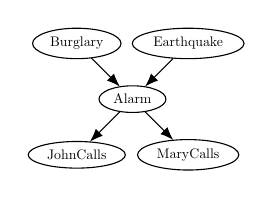
\begin{tikzpicture}[node distance=2cm,scale=0.5,every node/.style={scale=0.5}]
          \node[draw,ellipse] (alarm) {Alarm};
          \node[draw,ellipse,above left of=alarm] (burglary) {Burglary};
          \node[draw,ellipse,above right of=alarm] (earthquake) {Earthquake};
          \node[draw,ellipse,below left of=alarm] (johnCalls) {JohnCalls};
          \node[draw,ellipse,below right of=alarm] (maryCalls) {MaryCalls};
          \draw[-Latex] (burglary) -- (alarm);
          \draw[-Latex] (earthquake) -- (alarm);
          \draw[-Latex] (alarm) -- (johnCalls);
          \draw[-Latex] (alarm) -- (maryCalls);
        \end{tikzpicture}
      \end{block}
      \vspace{1cm}
      \begin{block}{Markov Random Field}
        \centering
        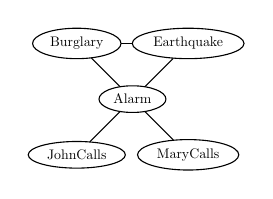
\begin{tikzpicture}[node distance=2cm,scale=0.5,every node/.style={scale=0.5}]
          \node[draw,ellipse] (alarm) {Alarm};
          \node[draw,ellipse,above left of=alarm] (burglary) {Burglary};
          \node[draw,ellipse,above right of=alarm] (earthquake) {Earthquake};
          \node[draw,ellipse,below left of=alarm] (johnCalls) {JohnCalls};
          \node[draw,ellipse,below right of=alarm] (maryCalls) {MaryCalls};
          \draw (burglary) -- (earthquake);
          \draw (burglary) -- (alarm);
          \draw (earthquake) -- (alarm);
          \draw (alarm) -- (johnCalls);
          \draw (alarm) -- (maryCalls);
        \end{tikzpicture}
      \end{block}
    \end{column}
  \end{columns}
  \onslide<2>{
    \begin{tikzpicture}[remember picture,overlay]
      \node[draw,star,fill=red!10] (wmc) at (current page.center) {WMC};
      \coordinate[xshift=-0.25\linewidth,yshift=-0.25\textheight] (p1) at (current page.center);
      \coordinate[xshift=0.25\linewidth,yshift=-0.25\textheight] (p2) at (current page.center);
      \coordinate[xshift=-0.25\linewidth,yshift=0.25\textheight] (p3) at (current page.center);
      \coordinate[xshift=0.25\linewidth,yshift=0.25\textheight] (p4) at (current page.center);
      \draw[-latex,line width=2pt,color=red!50] (p1) -- (wmc);
      \draw[-latex,line width=2pt,color=red!50] (p2) -- (wmc);
      \draw[-latex,line width=2pt,color=red!50] (p3) -- (wmc);
      \draw[-latex,line width=2pt,color=red!50] (p4) -- (wmc);
    \end{tikzpicture}
  }
\end{frame}

\begin{frame}[fragile]{Weighted Model Counting (WMC)}
  \begin{columns}
    \begin{column}{0.5\textwidth}
      \begin{itemize}
      \item Generalises propositional model counting ($\#\SAT{}$)
      \item Applications:
        \begin{itemize}
        \item graphical models
        \item probabilistic programming
        \item neural-symbolic artificial intelligence
        \end{itemize}
      \item Main types of algorithms:
        \begin{itemize}
        \item using knowledge compilation
        \item using a \SAT{} solver
        \item manipulating pseudo-Boolean functions
        \end{itemize}
      \end{itemize}
    \end{column}
    \begin{column}{0.5\textwidth}
      \begin{example}
      $w(x) = 0.3$, $w(\neg x) = 0.7$, $w(y) = 0.2$, $w(\neg y) = 0.8$
      \vspace{1cm}

      $\mathsf{WMC}(\alert{x \lor y}) = w(x)w(y) + w(x)w(\neg y) + w(\neg x)w(y)
      = 0.44$
      \end{example}
    \end{column}
  \end{columns}
\end{frame}

\begin{frame}
  \frametitle{Outline}
  \tableofcontents
\end{frame}

\section{An Alternative Formulation}

\begin{frame}{Formalising the Intuition from Before}
  For any propositional formula \structure{$\phi$} over a set of variables
  \structure{$X$} and \structure{$p, q \in \mathbb{R}$}, let
  \structure{$[\phi]^p_q\colon 2^X \to \mathbb{R}$} be the pseudo-Boolean
  function defined as
  \[
    [\phi]^p_q(Y) \coloneqq
    \begin{cases}
      p & \text{if } Y \models \phi \\
      q & \text{otherwise}
    \end{cases}
  \]
  for any \structure{$Y \subseteq X$}.

  \begin{definition}[Pseudo-Boolean Projection (PBP)]
    A \alert{PBP instance} is a tuple \structure{$(F, X, \omega)$}, where
    \structure{$X$} is the set of variables, \structure{$F$} is a set of
    two-valued pseudo-Boolean functions \structure{$2^X \to \mathbb{R}$}, and
    \structure{$\omega \in \mathbb{R}$} is the scaling factor.
  \end{definition}
\end{frame}

\begin{frame}{From WMC to PBP}
  The WMC instance has \structure{$x$} as the only \alert{indicator} variable
  and \structure{$p$}, \structure{$q$} as \alert{parameter} variables with
  weights \structure{$w(p) = 0.2$}, \structure{$w(q) = 0.8$}, and
  \structure{$w(\neg p) = w(\neg q) = 1$}.
  \begin{center}
    \begin{tabular}{llll}
      \toprule
      WMC Clause & \onslide<2->{In CNF} & \onslide<3->{Pseudo-Boolean Function} & \\
      \midrule
      $\neg x \Rightarrow p$ & \onslide<2->{$x \lor p$} & \onslide<3->{$[\neg x]_1^{0.2}$} & \\
      $p \Rightarrow \neg x$ & \onslide<2->{$\neg x \lor \neg p$} & & \onslide<4->{$[x]^{0.8}_{0.2}$} \\
      $x \Rightarrow q$ & \onslide<2->{$\neg x \lor q$} & \onslide<3->{$[x]_1^{0.8}$} & \\
      $q \Rightarrow x$ & \onslide<2->{$x \lor \neg q$} & & \\
      $\neg x$ & \onslide<2->{$\neg x$} & \onslide<3->{$[\neg x]_0^1$} & \onslide<4->{$[\neg x]_0^1$} \\
      \bottomrule
    \end{tabular}
  \end{center}
\end{frame}

\section{Correctness}

\section{Experimental Results}

\begin{frame}{Experimental Results}
  \centering
  % Created by tikzDevice version 0.12.3.1 on 2021-03-13 06:20:03
% !TEX encoding = UTF-8 Unicode
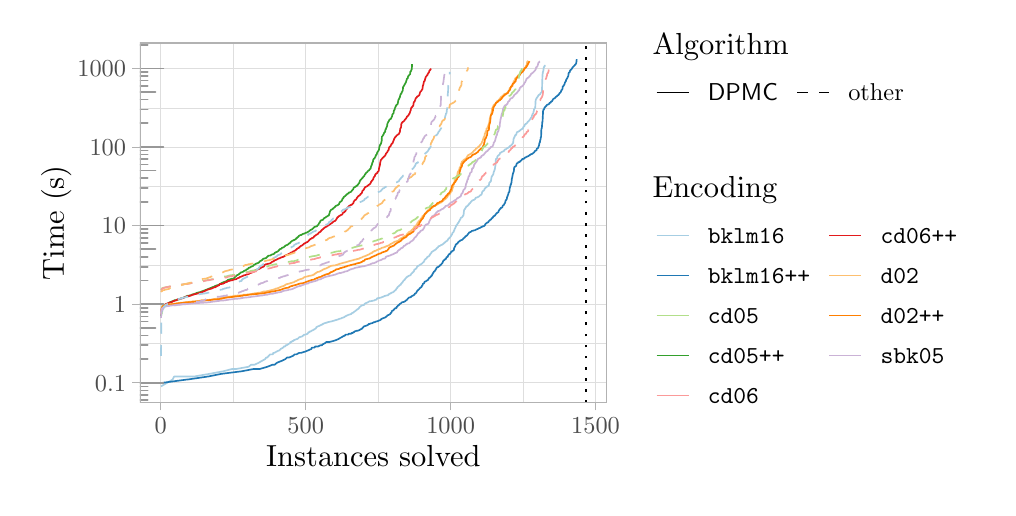
\begin{tikzpicture}[x=1pt,y=1pt]
\definecolor{fillColor}{RGB}{255,255,255}
\path[use as bounding box,fill=fillColor,fill opacity=0.00] (0,0) rectangle (346.90,166.22);
\begin{scope}
\path[clip] (  0.00,  0.00) rectangle (346.90,166.22);
\definecolor{drawColor}{RGB}{255,255,255}
\definecolor{fillColor}{RGB}{255,255,255}

\path[draw=drawColor,line width= 0.6pt,line join=round,line cap=round,fill=fillColor] (  0.00,  0.00) rectangle (346.90,166.22);
\end{scope}
\begin{scope}
\path[clip] ( 40.51, 30.69) rectangle (209.32,160.72);
\definecolor{fillColor}{RGB}{255,255,255}

\path[fill=fillColor] ( 40.51, 30.69) rectangle (209.32,160.72);
\definecolor{drawColor}{gray}{0.87}

\path[draw=drawColor,line width= 0.1pt,line join=round] ( 40.51, 52.10) --
	(209.32, 52.10);

\path[draw=drawColor,line width= 0.1pt,line join=round] ( 40.51, 80.50) --
	(209.32, 80.50);

\path[draw=drawColor,line width= 0.1pt,line join=round] ( 40.51,108.91) --
	(209.32,108.91);

\path[draw=drawColor,line width= 0.1pt,line join=round] ( 40.51,137.31) --
	(209.32,137.31);

\path[draw=drawColor,line width= 0.1pt,line join=round] ( 74.27, 30.69) --
	( 74.27,160.72);

\path[draw=drawColor,line width= 0.1pt,line join=round] (126.65, 30.69) --
	(126.65,160.72);

\path[draw=drawColor,line width= 0.1pt,line join=round] (179.02, 30.69) --
	(179.02,160.72);

\path[draw=drawColor,line width= 0.3pt,line join=round] ( 40.51, 37.90) --
	(209.32, 37.90);

\path[draw=drawColor,line width= 0.3pt,line join=round] ( 40.51, 66.30) --
	(209.32, 66.30);

\path[draw=drawColor,line width= 0.3pt,line join=round] ( 40.51, 94.71) --
	(209.32, 94.71);

\path[draw=drawColor,line width= 0.3pt,line join=round] ( 40.51,123.11) --
	(209.32,123.11);

\path[draw=drawColor,line width= 0.3pt,line join=round] ( 40.51,151.51) --
	(209.32,151.51);

\path[draw=drawColor,line width= 0.3pt,line join=round] ( 48.08, 30.69) --
	( 48.08,160.72);

\path[draw=drawColor,line width= 0.3pt,line join=round] (100.46, 30.69) --
	(100.46,160.72);

\path[draw=drawColor,line width= 0.3pt,line join=round] (152.83, 30.69) --
	(152.83,160.72);

\path[draw=drawColor,line width= 0.3pt,line join=round] (205.21, 30.69) --
	(205.21,160.72);
\definecolor{drawColor}{RGB}{166,206,227}

\path[draw=drawColor,line width= 0.6pt,line join=round] ( 48.18, 36.60) --
	( 52.37, 39.07) --
	( 52.90, 40.15) --
	( 60.02, 40.15) --
	( 65.68, 41.13) --
	( 70.60, 42.05) --
	( 73.95, 42.90) --
	( 75.42, 42.90) --
	( 79.82, 43.69) --
	( 80.76, 44.44) --
	( 82.02, 44.44) --
	( 83.49, 45.15) --
	( 84.64, 45.81) --
	( 85.79, 46.45) --
	( 86.21, 47.05) --
	( 86.63, 47.05) --
	( 87.05, 47.62) --
	( 87.15, 47.62) --
	( 87.57, 48.17) --
	( 88.62, 48.17) --
	( 88.72, 48.70) --
	( 89.14, 48.70) --
	( 89.98, 49.20) --
	( 91.03, 49.68) --
	( 91.45, 50.15) --
	( 92.29, 50.60) --
	( 92.60, 51.03) --
	( 93.02, 51.03) --
	( 93.23, 51.45) --
	( 93.54, 51.45) --
	( 94.17, 51.85) --
	( 94.80, 52.24) --
	( 94.90, 52.62) --
	( 95.32, 52.62) --
	( 95.64, 52.99) --
	( 95.95, 52.99) --
	( 96.27, 53.35) --
	( 96.37, 53.35) --
	( 97.21, 53.70) --
	( 97.42, 53.70) --
	( 97.84, 54.04) --
	( 98.15, 54.36) --
	( 99.30, 54.69) --
	( 99.51, 55.00) --
	( 99.62, 55.00) --
	( 99.93, 55.30) --
	(100.35, 55.30) --
	(101.08, 55.60) --
	(101.19, 55.60) --
	(101.29, 55.89) --
	(101.50, 56.17) --
	(101.82, 56.17) --
	(101.92, 56.45) --
	(102.34, 56.45) --
	(102.55, 56.72) --
	(102.66, 56.72) --
	(103.18, 56.99) --
	(103.28, 56.99) --
	(103.60, 57.25) --
	(104.12, 57.50) --
	(104.23, 57.75) --
	(104.33, 57.99) --
	(104.75, 58.23) --
	(105.38, 58.47) --
	(105.80, 58.70) --
	(106.43, 58.93) --
	(106.53, 59.15) --
	(106.85, 59.15) --
	(106.95, 59.37) --
	(107.16, 59.37) --
	(107.79, 59.58) --
	(108.10, 59.58) --
	(108.21, 59.79) --
	(108.42, 59.79) --
	(109.36, 60.00) --
	(109.47, 60.00) --
	(110.20, 60.20) --
	(110.83, 60.40) --
	(111.46, 60.60) --
	(111.56, 60.60) --
	(112.19, 60.80) --
	(112.61, 60.99) --
	(113.34, 61.18) --
	(113.55, 61.36) --
	(113.76, 61.36) --
	(114.18, 61.54) --
	(114.28, 61.54) --
	(114.49, 61.72) --
	(114.60, 61.72) --
	(114.70, 61.90) --
	(115.12, 62.08) --
	(115.44, 62.25) --
	(115.86, 62.42) --
	(116.38, 62.59) --
	(116.90, 62.75) --
	(117.01, 62.92) --
	(117.22, 63.08) --
	(117.64, 63.24) --
	(117.74, 63.39) --
	(117.85, 63.39) --
	(117.95, 63.55) --
	(118.16, 63.70) --
	(118.26, 63.70) --
	(118.37, 63.85) --
	(118.47, 63.85) --
	(118.58, 64.00) --
	(118.79, 64.15) --
	(119.00, 64.30) --
	(119.10, 64.44) --
	(119.42, 64.58) --
	(119.63, 64.72) --
	(119.84, 65.14) --
	(119.94, 65.27) --
	(120.36, 65.54) --
	(120.46, 65.67) --
	(120.57, 65.80) --
	(121.09, 65.93) --
	(121.62, 66.05) --
	(121.72, 66.42) --
	(122.04, 66.55) --
	(122.14, 66.67) --
	(122.46, 66.78) --
	(122.77, 66.90) --
	(122.98, 67.02) --
	(123.08, 67.14) --
	(123.19, 67.14) --
	(123.40, 67.36) --
	(123.71, 67.36) --
	(124.55, 67.48) --
	(124.76, 67.59) --
	(125.07, 67.59) --
	(125.28, 67.70) --
	(125.49, 67.81) --
	(125.81, 67.92) --
	(125.91, 67.92) --
	(126.12, 68.02) --
	(126.23, 68.34) --
	(126.33, 68.45) --
	(126.44, 68.45) --
	(126.96, 68.55) --
	(127.06, 68.55) --
	(127.38, 68.65) --
	(127.48, 68.65) --
	(127.90, 68.75) --
	(128.01, 68.85) --
	(128.32, 68.95) --
	(128.64, 69.05) --
	(128.74, 69.15) --
	(128.95, 69.25) --
	(129.37, 69.35) --
	(129.47, 69.44) --
	(129.79, 69.44) --
	(130.00, 69.54) --
	(130.31, 69.54) --
	(130.42, 69.82) --
	(130.63, 70.00) --
	(130.94, 70.09) --
	(131.04, 70.18) --
	(131.15, 70.18) --
	(131.25, 70.27) --
	(131.36, 70.36) --
	(131.46, 70.45) --
	(131.78, 70.54) --
	(131.88, 70.54) --
	(132.09, 70.71) --
	(132.20, 70.71) --
	(132.30, 70.80) --
	(132.41, 70.97) --
	(132.62, 71.14) --
	(132.72, 71.22) --
	(132.83, 71.38) --
	(133.04, 71.47) --
	(133.14, 71.55) --
	(133.24, 71.94) --
	(133.45, 72.10) --
	(133.56, 72.18) --
	(133.66, 72.48) --
	(133.77, 72.55) --
	(133.98, 72.70) --
	(134.08, 72.77) --
	(134.19, 72.92) --
	(134.29, 72.99) --
	(134.40, 73.13) --
	(134.50, 73.20) --
	(134.61, 73.27) --
	(134.82, 73.34) --
	(134.92, 73.69) --
	(135.03, 73.76) --
	(135.13, 73.96) --
	(135.34, 74.02) --
	(135.44, 74.28) --
	(135.55, 74.35) --
	(135.65, 74.60) --
	(135.76, 74.73) --
	(135.86, 74.85) --
	(135.97, 74.91) --
	(136.18, 75.10) --
	(136.28, 75.16) --
	(136.39, 75.45) --
	(136.49, 75.51) --
	(136.60, 75.69) --
	(136.70, 75.74) --
	(136.81, 75.91) --
	(136.91, 76.03) --
	(137.12, 76.14) --
	(137.23, 76.19) --
	(137.33, 76.36) --
	(137.54, 76.41) --
	(137.64, 76.52) --
	(137.75, 76.58) --
	(137.96, 76.63) --
	(138.06, 76.68) --
	(138.27, 76.74) --
	(138.38, 76.84) --
	(138.69, 77.41) --
	(138.80, 77.46) --
	(138.90, 77.51) --
	(139.01, 77.65) --
	(139.11, 77.75) --
	(139.22, 77.90) --
	(139.32, 77.94) --
	(139.53, 78.09) --
	(139.63, 78.42) --
	(139.74, 78.78) --
	(139.84, 78.82) --
	(139.95, 78.87) --
	(140.05, 78.96) --
	(140.16, 79.05) --
	(140.26, 79.09) --
	(140.37, 79.18) --
	(140.47, 79.22) --
	(140.58, 79.56) --
	(140.68, 79.77) --
	(140.79, 79.94) --
	(140.89, 79.98) --
	(141.00, 80.10) --
	(141.10, 80.18) --
	(141.21, 80.18) --
	(141.31, 80.22) --
	(141.42, 80.30) --
	(141.52, 80.34) --
	(141.63, 80.38) --
	(141.73, 80.49) --
	(141.83, 80.61) --
	(141.94, 80.69) --
	(142.15, 80.73) --
	(142.25, 80.84) --
	(142.36, 80.88) --
	(142.46, 80.95) --
	(142.67, 81.21) --
	(142.78, 81.32) --
	(142.88, 81.40) --
	(142.99, 81.47) --
	(143.09, 81.47) --
	(143.20, 81.75) --
	(143.30, 81.93) --
	(143.41, 82.20) --
	(143.51, 82.44) --
	(143.62, 82.47) --
	(143.72, 82.54) --
	(143.83, 82.67) --
	(143.93, 82.70) --
	(144.03, 82.77) --
	(144.14, 82.80) --
	(144.24, 83.09) --
	(144.35, 83.28) --
	(144.45, 83.31) --
	(144.56, 83.49) --
	(144.87, 83.52) --
	(144.98, 83.62) --
	(145.08, 83.80) --
	(145.19, 83.92) --
	(145.29, 84.00) --
	(145.40, 84.35) --
	(145.50, 84.44) --
	(145.61, 84.55) --
	(145.71, 84.63) --
	(145.82, 84.77) --
	(145.92, 85.15) --
	(146.13, 85.18) --
	(146.23, 85.29) --
	(146.34, 85.39) --
	(146.44, 85.42) --
	(146.55, 85.55) --
	(146.65, 85.60) --
	(146.76, 85.68) --
	(146.86, 85.70) --
	(146.97, 85.73) --
	(147.07, 85.80) --
	(147.18, 85.91) --
	(147.28, 85.93) --
	(147.39, 86.08) --
	(147.49, 86.13) --
	(147.60, 86.15) --
	(147.70, 86.47) --
	(147.81, 86.50) --
	(147.91, 86.59) --
	(148.02, 86.69) --
	(148.12, 86.71) --
	(148.22, 86.80) --
	(148.33, 87.04) --
	(148.43, 87.24) --
	(148.54, 87.26) --
	(148.64, 87.29) --
	(148.75, 87.31) --
	(148.85, 87.33) --
	(148.96, 87.40) --
	(149.06, 87.40) --
	(149.17, 87.53) --
	(149.27, 87.57) --
	(149.38, 87.68) --
	(149.48, 87.71) --
	(149.59, 87.73) --
	(149.69, 87.79) --
	(149.80, 87.81) --
	(149.90, 87.94) --
	(150.01, 87.99) --
	(150.11, 88.05) --
	(150.22, 88.09) --
	(150.32, 88.22) --
	(150.42, 88.40) --
	(150.63, 88.42) --
	(150.74, 88.61) --
	(150.84, 88.71) --
	(150.95, 88.77) --
	(151.05, 88.93) --
	(151.16, 88.97) --
	(151.26, 88.99) --
	(151.37, 89.08) --
	(151.47, 89.12) --
	(151.58, 89.24) --
	(151.68, 89.32) --
	(151.79, 89.54) --
	(151.89, 89.60) --
	(152.00, 89.93) --
	(152.10, 89.97) --
	(152.21, 90.00) --
	(152.42, 90.34) --
	(152.62, 90.38) --
	(152.73, 90.60) --
	(152.83, 90.70) --
	(152.94, 90.87) --
	(153.04, 91.22) --
	(153.15, 91.24) --
	(153.25, 91.38) --
	(153.36, 91.50) --
	(153.46, 92.04) --
	(153.57, 92.11) --
	(153.67, 92.21) --
	(153.78, 92.29) --
	(153.88, 92.30) --
	(153.99, 92.74) --
	(154.09, 92.87) --
	(154.20, 93.11) --
	(154.30, 93.56) --
	(154.41, 93.58) --
	(154.51, 93.90) --
	(154.61, 94.16) --
	(154.72, 94.19) --
	(154.82, 94.72) --
	(155.03, 94.83) --
	(155.14, 95.02) --
	(155.24, 95.08) --
	(155.35, 95.51) --
	(155.45, 95.53) --
	(155.56, 95.67) --
	(155.66, 95.77) --
	(155.77, 95.93) --
	(155.87, 96.21) --
	(155.98, 96.34) --
	(156.08, 96.63) --
	(156.19, 96.71) --
	(156.29, 96.95) --
	(156.40, 97.06) --
	(156.50, 97.48) --
	(156.61, 97.55) --
	(156.71, 97.59) --
	(156.81, 97.62) --
	(156.92, 97.67) --
	(157.02, 97.85) --
	(157.13, 97.88) --
	(157.23, 98.03) --
	(157.34, 98.32) --
	(157.44, 98.34) --
	(157.55, 98.94) --
	(157.65, 99.96) --
	(157.76,100.50) --
	(157.86,100.51) --
	(157.97,100.69) --
	(158.07,100.76) --
	(158.18,101.05) --
	(158.28,101.21) --
	(158.39,101.35) --
	(158.49,101.61) --
	(158.60,101.64) --
	(158.70,101.67) --
	(158.81,101.71) --
	(158.91,101.81) --
	(159.01,101.93) --
	(159.12,101.95) --
	(159.22,102.19) --
	(159.33,102.24) --
	(159.43,102.33) --
	(159.54,102.67) --
	(159.64,102.69) --
	(159.75,102.70) --
	(159.85,102.82) --
	(159.96,102.99) --
	(160.06,103.06) --
	(160.17,103.27) --
	(160.27,103.38) --
	(160.38,103.52) --
	(160.48,103.55) --
	(160.59,103.70) --
	(160.69,103.80) --
	(160.80,103.81) --
	(160.90,103.90) --
	(161.01,103.93) --
	(161.11,103.95) --
	(161.21,104.00) --
	(161.32,104.02) --
	(161.42,104.09) --
	(161.53,104.23) --
	(161.63,104.24) --
	(161.74,104.44) --
	(161.84,104.63) --
	(161.95,104.80) --
	(162.05,104.81) --
	(162.16,104.83) --
	(162.26,104.85) --
	(162.47,104.90) --
	(162.58,104.92) --
	(162.68,105.04) --
	(162.79,105.05) --
	(162.89,105.11) --
	(163.00,105.18) --
	(163.10,105.25) --
	(163.20,105.30) --
	(163.31,105.45) --
	(163.41,105.57) --
	(163.52,105.65) --
	(163.62,105.72) --
	(163.73,105.77) --
	(163.83,105.79) --
	(163.94,105.90) --
	(164.04,106.03) --
	(164.15,106.46) --
	(164.25,106.85) --
	(164.36,107.01) --
	(164.46,107.11) --
	(164.57,107.21) --
	(164.67,107.30) --
	(164.78,107.35) --
	(164.88,107.43) --
	(164.99,107.55) --
	(165.09,107.95) --
	(165.20,107.99) --
	(165.30,108.29) --
	(165.40,108.32) --
	(165.51,108.34) --
	(165.61,108.56) --
	(165.72,108.57) --
	(165.82,108.59) --
	(165.93,108.77) --
	(166.03,108.90) --
	(166.14,108.92) --
	(166.24,108.93) --
	(166.35,108.97) --
	(166.45,109.00) --
	(166.56,109.07) --
	(166.66,109.25) --
	(166.77,110.06) --
	(166.87,110.25) --
	(166.98,110.26) --
	(167.08,110.48) --
	(167.19,110.51) --
	(167.29,110.53) --
	(167.40,110.88) --
	(167.50,111.51) --
	(167.60,112.18) --
	(167.71,112.46) --
	(167.81,112.57) --
	(167.92,112.78) --
	(168.02,112.93) --
	(168.13,113.05) --
	(168.23,113.19) --
	(168.34,113.75) --
	(168.44,114.16) --
	(168.55,114.34) --
	(168.65,114.71) --
	(168.76,114.86) --
	(168.86,115.40) --
	(168.97,116.25) --
	(169.07,116.58) --
	(169.18,118.67) --
	(169.28,118.80) --
	(169.39,118.83) --
	(169.49,118.87) --
	(169.59,118.95) --
	(169.70,119.57) --
	(169.80,119.71) --
	(169.91,119.90) --
	(170.01,120.00) --
	(170.12,120.07) --
	(170.22,120.17) --
	(170.33,120.20) --
	(170.43,120.31) --
	(170.54,120.44) --
	(170.64,120.79) --
	(170.75,120.97) --
	(170.85,121.04) --
	(170.96,121.06) --
	(171.06,121.17) --
	(171.17,121.17) --
	(171.27,121.28) --
	(171.38,121.31) --
	(171.48,121.35) --
	(171.59,121.46) --
	(171.69,121.48) --
	(171.79,121.51) --
	(171.90,121.57) --
	(172.00,121.58) --
	(172.11,121.70) --
	(172.21,121.85) --
	(172.32,122.11) --
	(172.42,122.19) --
	(172.53,122.22) --
	(172.63,122.23) --
	(172.74,122.29) --
	(172.84,122.30) --
	(172.95,122.44) --
	(173.05,122.45) --
	(173.16,122.61) --
	(173.26,122.72) --
	(173.37,122.72) --
	(173.47,122.75) --
	(173.58,122.79) --
	(173.68,122.90) --
	(173.79,122.95) --
	(173.89,122.99) --
	(173.99,123.09) --
	(174.10,123.23) --
	(174.20,123.29) --
	(174.31,123.46) --
	(174.41,123.50) --
	(174.52,123.51) --
	(174.62,123.69) --
	(174.73,123.75) --
	(174.83,123.77) --
	(174.94,123.94) --
	(175.04,124.06) --
	(175.15,124.25) --
	(175.25,124.37) --
	(175.36,124.46) --
	(175.46,124.88) --
	(175.57,125.99) --
	(175.67,126.22) --
	(175.78,126.43) --
	(175.88,126.74) --
	(175.99,126.85) --
	(176.09,127.12) --
	(176.19,127.43) --
	(176.30,127.44) --
	(176.40,127.45) --
	(176.51,127.48) --
	(176.61,127.88) --
	(176.72,128.25) --
	(176.82,128.46) --
	(176.93,128.52) --
	(177.03,128.59) --
	(177.24,128.59) --
	(177.35,128.67) --
	(177.45,128.79) --
	(177.56,128.80) --
	(177.66,128.84) --
	(177.77,128.99) --
	(177.87,129.02) --
	(177.98,129.15) --
	(178.08,129.29) --
	(178.18,129.36) --
	(178.29,129.38) --
	(178.39,129.44) --
	(178.50,129.53) --
	(178.60,129.59) --
	(178.71,129.64) --
	(178.81,129.68) --
	(178.92,129.85) --
	(179.02,130.04) --
	(179.13,130.33) --
	(179.23,130.46) --
	(179.34,130.59) --
	(179.44,130.65) --
	(179.55,130.65) --
	(179.65,131.11) --
	(179.76,131.29) --
	(179.86,131.35) --
	(179.97,131.45) --
	(180.07,131.46) --
	(180.18,131.56) --
	(180.28,131.56) --
	(180.38,131.77) --
	(180.49,131.82) --
	(180.59,132.04) --
	(180.70,132.17) --
	(180.80,132.28) --
	(180.91,132.35) --
	(181.01,132.44) --
	(181.12,132.55) --
	(181.22,132.66) --
	(181.33,132.83) --
	(181.43,132.95) --
	(181.54,133.21) --
	(181.64,133.22) --
	(181.75,133.47) --
	(181.85,133.61) --
	(181.96,133.75) --
	(182.06,133.89) --
	(182.17,134.05) --
	(182.27,134.59) --
	(182.38,134.83) --
	(182.48,135.05) --
	(182.58,135.12) --
	(182.69,135.22) --
	(182.79,135.91) --
	(182.90,136.10) --
	(183.00,136.84) --
	(183.11,136.88) --
	(183.21,137.06) --
	(183.32,137.16) --
	(183.42,137.47) --
	(183.53,139.73) --
	(183.63,140.25) --
	(183.74,140.39) --
	(183.84,140.53) --
	(183.95,140.91) --
	(184.05,140.96) --
	(184.16,140.96) --
	(184.26,141.31) --
	(184.37,141.37) --
	(184.47,141.68) --
	(184.57,141.75) --
	(184.68,141.82) --
	(184.78,142.02) --
	(184.89,142.04) --
	(184.99,142.08) --
	(185.10,142.10) --
	(185.20,142.18) --
	(185.31,142.56) --
	(185.41,142.60) --
	(185.52,142.75) --
	(185.62,142.83) --
	(185.73,143.02) --
	(185.83,143.07) --
	(185.94,147.02) --
	(186.04,149.16) --
	(186.15,150.01) --
	(186.25,150.41) --
	(186.36,150.79) --
	(186.46,151.75) --
	(186.57,151.92) --
	(186.67,152.18) --
	(186.77,152.34) --
	(186.88,152.44) --
	(186.98,152.54) --
	(187.09,152.60);
\definecolor{drawColor}{RGB}{31,120,180}

\path[draw=drawColor,line width= 0.6pt,line join=round] ( 48.81, 37.90) --
	( 57.51, 39.07) --
	( 57.72, 39.07) --
	( 65.05, 40.15) --
	( 65.15, 40.15) --
	( 69.97, 41.13) --
	( 77.31, 42.05) --
	( 81.71, 42.90) --
	( 83.91, 42.90) --
	( 86.63, 43.69) --
	( 88.51, 44.44) --
	( 89.25, 44.44) --
	( 90.09, 45.15) --
	( 91.76, 45.81) --
	( 93.12, 46.45) --
	( 93.75, 47.05) --
	( 94.49, 47.05) --
	( 95.85, 47.62) --
	( 96.48, 48.17) --
	( 97.10, 48.17) --
	( 98.15, 48.70) --
	( 98.78, 48.70) --
	(100.35, 49.20) --
	(101.50, 49.68) --
	(102.55, 50.15) --
	(102.66, 50.60) --
	(103.60, 50.60) --
	(103.91, 51.03) --
	(104.96, 51.03) --
	(105.80, 51.45) --
	(106.32, 51.45) --
	(106.64, 51.85) --
	(106.74, 51.85) --
	(107.48, 52.24) --
	(107.89, 52.62) --
	(108.94, 52.62) --
	(110.41, 52.99) --
	(111.46, 53.35) --
	(112.29, 53.70) --
	(112.82, 54.04) --
	(113.45, 54.36) --
	(113.97, 54.69) --
	(114.70, 55.00) --
	(114.81, 55.30) --
	(115.86, 55.30) --
	(115.96, 55.60) --
	(116.90, 55.60) --
	(117.01, 55.89) --
	(117.43, 55.89) --
	(117.64, 56.17) --
	(117.95, 56.17) --
	(118.06, 56.45) --
	(118.16, 56.45) --
	(119.00, 56.72) --
	(119.31, 56.72) --
	(119.94, 56.99) --
	(120.05, 56.99) --
	(120.26, 57.25) --
	(120.36, 57.25) --
	(120.88, 57.50) --
	(120.99, 57.75) --
	(121.30, 57.99) --
	(121.41, 58.23) --
	(122.14, 58.47) --
	(122.77, 58.70) --
	(123.08, 58.93) --
	(123.19, 59.15) --
	(123.61, 59.15) --
	(123.92, 59.37) --
	(124.24, 59.37) --
	(124.76, 59.58) --
	(125.07, 59.79) --
	(125.28, 59.79) --
	(125.81, 60.00) --
	(126.54, 60.20) --
	(126.96, 60.40) --
	(127.48, 60.60) --
	(127.69, 60.80) --
	(127.80, 60.99) --
	(128.32, 61.18) --
	(128.74, 61.36) --
	(128.95, 61.36) --
	(129.16, 61.54) --
	(129.47, 61.72) --
	(129.68, 61.90) --
	(129.89, 62.08) --
	(130.00, 62.25) --
	(130.42, 62.42) --
	(130.73, 62.59) --
	(131.04, 62.75) --
	(131.15, 63.08) --
	(131.46, 63.24) --
	(131.57, 63.85) --
	(131.78, 63.85) --
	(131.88, 64.00) --
	(132.09, 64.00) --
	(132.20, 64.15) --
	(132.30, 64.30) --
	(132.41, 64.44) --
	(132.62, 64.72) --
	(132.93, 64.86) --
	(133.14, 64.86) --
	(133.24, 64.86) --
	(133.35, 65.41) --
	(133.56, 65.41) --
	(133.66, 65.54) --
	(133.77, 65.80) --
	(133.98, 65.93) --
	(134.08, 65.93) --
	(134.19, 66.05) --
	(134.40, 66.30) --
	(134.50, 66.42) --
	(134.82, 66.55) --
	(135.03, 66.78) --
	(135.13, 66.90) --
	(135.44, 67.02) --
	(135.97, 67.14) --
	(136.18, 67.25) --
	(136.39, 67.36) --
	(136.60, 67.59) --
	(136.81, 67.70) --
	(136.91, 67.81) --
	(137.02, 67.81) --
	(137.23, 68.13) --
	(137.33, 68.24) --
	(137.44, 68.34) --
	(137.54, 68.45) --
	(137.64, 68.55) --
	(137.75, 68.65) --
	(137.96, 68.75) --
	(138.48, 68.85) --
	(138.59, 69.05) --
	(138.69, 69.15) --
	(138.90, 69.25) --
	(139.11, 69.35) --
	(139.22, 69.44) --
	(139.43, 69.54) --
	(139.63, 69.63) --
	(139.74, 69.73) --
	(139.84, 69.91) --
	(139.95, 70.18) --
	(140.16, 70.18) --
	(140.37, 70.36) --
	(140.47, 70.54) --
	(140.58, 70.80) --
	(140.68, 70.97) --
	(140.79, 71.14) --
	(140.89, 71.22) --
	(141.00, 71.30) --
	(141.10, 71.47) --
	(141.21, 71.55) --
	(141.31, 71.63) --
	(141.42, 71.71) --
	(141.52, 71.79) --
	(141.63, 72.02) --
	(141.73, 72.10) --
	(141.83, 72.18) --
	(142.15, 72.40) --
	(142.25, 72.48) --
	(142.36, 72.63) --
	(142.46, 72.92) --
	(142.57, 72.99) --
	(142.67, 73.06) --
	(142.78, 73.62) --
	(142.99, 73.69) --
	(143.09, 73.76) --
	(143.20, 73.89) --
	(143.30, 74.02) --
	(143.41, 74.35) --
	(143.51, 74.41) --
	(143.62, 74.48) --
	(143.83, 74.54) --
	(143.93, 74.60) --
	(144.03, 74.66) --
	(144.14, 74.79) --
	(144.24, 74.85) --
	(144.35, 74.91) --
	(144.45, 74.91) --
	(144.66, 75.10) --
	(144.77, 75.22) --
	(144.87, 75.51) --
	(144.98, 75.69) --
	(145.08, 75.74) --
	(145.19, 75.80) --
	(145.29, 75.91) --
	(145.50, 76.03) --
	(145.61, 76.25) --
	(145.71, 76.30) --
	(145.82, 76.47) --
	(145.92, 76.52) --
	(146.03, 76.58) --
	(146.23, 77.15) --
	(146.34, 77.20) --
	(146.44, 77.51) --
	(146.55, 77.60) --
	(146.65, 77.70) --
	(146.76, 78.04) --
	(146.97, 78.18) --
	(147.18, 78.32) --
	(147.28, 78.55) --
	(147.39, 78.60) --
	(147.49, 79.00) --
	(147.60, 79.05) --
	(147.70, 79.26) --
	(147.81, 79.56) --
	(147.91, 79.56) --
	(148.02, 79.65) --
	(148.22, 79.69) --
	(148.33, 79.73) --
	(148.43, 79.89) --
	(148.54, 79.89) --
	(148.64, 79.98) --
	(148.75, 80.06) --
	(148.85, 80.06) --
	(148.96, 80.30) --
	(149.06, 80.42) --
	(149.17, 80.46) --
	(149.27, 80.49) --
	(149.38, 80.53) --
	(149.48, 80.80) --
	(149.69, 80.99) --
	(149.80, 81.18) --
	(149.90, 81.18) --
	(150.01, 81.54) --
	(150.11, 81.79) --
	(150.22, 82.00) --
	(150.42, 82.20) --
	(150.53, 82.24) --
	(150.63, 82.24) --
	(150.74, 82.51) --
	(150.84, 82.54) --
	(150.95, 82.57) --
	(151.05, 82.67) --
	(151.16, 82.74) --
	(151.26, 83.03) --
	(151.37, 83.31) --
	(151.58, 83.34) --
	(151.68, 83.37) --
	(151.79, 83.40) --
	(151.89, 83.80) --
	(152.00, 84.03) --
	(152.10, 84.06) --
	(152.21, 84.35) --
	(152.31, 84.38) --
	(152.42, 84.41) --
	(152.52, 84.47) --
	(152.62, 84.52) --
	(152.73, 84.55) --
	(152.83, 84.80) --
	(152.94, 85.13) --
	(153.04, 85.15) --
	(153.15, 85.18) --
	(153.25, 85.31) --
	(153.36, 85.44) --
	(153.46, 85.55) --
	(153.67, 85.60) --
	(153.78, 85.68) --
	(153.99, 85.80) --
	(154.09, 86.54) --
	(154.20, 86.71) --
	(154.30, 86.87) --
	(154.41, 87.13) --
	(154.51, 87.17) --
	(154.61, 87.68) --
	(154.72, 87.86) --
	(154.82, 87.96) --
	(154.93, 88.01) --
	(155.03, 88.07) --
	(155.14, 88.20) --
	(155.24, 88.22) --
	(155.35, 88.24) --
	(155.45, 88.59) --
	(155.56, 88.63) --
	(155.66, 88.83) --
	(155.77, 88.87) --
	(155.87, 88.95) --
	(155.98, 89.01) --
	(156.08, 89.04) --
	(156.19, 89.14) --
	(156.29, 89.33) --
	(156.40, 89.33) --
	(156.50, 89.37) --
	(156.61, 89.41) --
	(156.71, 89.43) --
	(156.81, 89.47) --
	(156.92, 89.52) --
	(157.02, 89.56) --
	(157.13, 89.65) --
	(157.23, 89.80) --
	(157.34, 89.82) --
	(157.44, 90.09) --
	(157.55, 90.11) --
	(157.65, 90.22) --
	(157.76, 90.31) --
	(157.86, 90.36) --
	(157.97, 90.52) --
	(158.07, 90.53) --
	(158.18, 90.79) --
	(158.28, 90.89) --
	(158.39, 90.91) --
	(158.49, 90.97) --
	(158.60, 91.06) --
	(158.70, 91.09) --
	(158.81, 91.17) --
	(158.91, 91.37) --
	(159.01, 91.48) --
	(159.12, 91.69) --
	(159.22, 91.78) --
	(159.33, 91.88) --
	(159.43, 92.01) --
	(159.54, 92.26) --
	(159.64, 92.27) --
	(159.75, 92.30) --
	(159.96, 92.36) --
	(160.06, 92.39) --
	(160.17, 92.42) --
	(160.27, 92.53) --
	(160.38, 92.69) --
	(160.48, 92.76) --
	(160.59, 92.79) --
	(160.69, 92.80) --
	(160.80, 92.82) --
	(160.90, 92.84) --
	(161.01, 92.89) --
	(161.11, 92.93) --
	(161.21, 92.96) --
	(161.53, 92.99) --
	(161.63, 93.00) --
	(161.74, 93.11) --
	(161.84, 93.13) --
	(161.95, 93.23) --
	(162.05, 93.27) --
	(162.16, 93.31) --
	(162.26, 93.36) --
	(162.37, 93.41) --
	(162.47, 93.42) --
	(162.58, 93.46) --
	(162.68, 93.57) --
	(162.79, 93.57) --
	(162.89, 93.60) --
	(163.00, 93.73) --
	(163.10, 93.77) --
	(163.20, 93.80) --
	(163.31, 93.81) --
	(163.41, 93.85) --
	(163.52, 93.90) --
	(163.62, 93.97) --
	(163.73, 94.06) --
	(163.83, 94.12) --
	(163.94, 94.15) --
	(164.04, 94.27) --
	(164.25, 94.27) --
	(164.36, 94.35) --
	(164.46, 94.42) --
	(164.57, 94.47) --
	(164.67, 94.47) --
	(164.78, 94.48) --
	(164.88, 94.52) --
	(164.99, 94.61) --
	(165.09, 94.64) --
	(165.20, 94.83) --
	(165.30, 94.95) --
	(165.40, 95.24) --
	(165.51, 95.41) --
	(165.61, 95.42) --
	(165.72, 95.59) --
	(165.93, 95.62) --
	(166.03, 95.80) --
	(166.14, 95.84) --
	(166.24, 95.86) --
	(166.35, 95.88) --
	(166.45, 95.95) --
	(166.56, 96.23) --
	(166.66, 96.32) --
	(166.77, 96.43) --
	(166.87, 96.46) --
	(166.98, 96.61) --
	(167.08, 96.76) --
	(167.19, 96.78) --
	(167.29, 96.82) --
	(167.40, 96.89) --
	(167.50, 96.93) --
	(167.60, 97.28) --
	(167.71, 97.33) --
	(167.81, 97.45) --
	(167.92, 97.48) --
	(168.02, 97.54) --
	(168.13, 97.63) --
	(168.23, 97.97) --
	(168.34, 98.05) --
	(168.44, 98.13) --
	(168.55, 98.15) --
	(168.65, 98.20) --
	(168.76, 98.27) --
	(168.86, 98.35) --
	(168.97, 98.58) --
	(169.07, 98.65) --
	(169.18, 98.88) --
	(169.28, 98.90) --
	(169.39, 99.16) --
	(169.49, 99.19) --
	(169.59, 99.21) --
	(169.70, 99.34) --
	(169.80, 99.38) --
	(169.91, 99.49) --
	(170.01, 99.52) --
	(170.12, 99.61) --
	(170.22,100.10) --
	(170.33,100.11) --
	(170.43,100.40) --
	(170.54,100.52) --
	(170.64,100.68) --
	(170.75,100.71) --
	(170.85,100.81) --
	(170.96,101.09) --
	(171.06,101.12) --
	(171.17,101.13) --
	(171.27,101.20) --
	(171.38,101.25) --
	(171.48,101.26) --
	(171.59,101.56) --
	(171.69,101.98) --
	(171.79,101.99) --
	(171.90,102.09) --
	(172.00,102.14) --
	(172.11,102.19) --
	(172.21,102.39) --
	(172.32,102.75) --
	(172.42,102.76) --
	(172.53,103.00) --
	(172.63,103.54) --
	(172.74,103.82) --
	(172.84,103.92) --
	(172.95,103.96) --
	(173.05,104.19) --
	(173.16,104.47) --
	(173.26,105.15) --
	(173.37,105.17) --
	(173.47,105.66) --
	(173.58,105.71) --
	(173.68,106.14) --
	(173.79,106.68) --
	(173.89,106.69) --
	(173.99,106.86) --
	(174.10,107.20) --
	(174.20,108.49) --
	(174.31,108.55) --
	(174.41,108.96) --
	(174.52,109.49) --
	(174.62,109.56) --
	(174.73,110.00) --
	(174.83,110.29) --
	(174.94,111.55) --
	(175.04,111.92) --
	(175.15,112.47) --
	(175.25,112.99) --
	(175.36,113.54) --
	(175.46,113.79) --
	(175.57,114.04) --
	(175.67,114.31) --
	(175.78,115.60) --
	(175.88,115.80) --
	(175.99,115.87) --
	(176.09,116.01) --
	(176.19,116.08) --
	(176.30,116.13) --
	(176.40,116.20) --
	(176.51,116.28) --
	(176.61,116.79) --
	(176.72,117.06) --
	(176.82,117.25) --
	(176.93,117.25) --
	(177.03,117.29) --
	(177.14,117.33) --
	(177.24,117.64) --
	(177.45,117.65) --
	(177.56,117.69) --
	(177.66,117.69) --
	(177.77,117.70) --
	(177.87,117.80) --
	(177.98,118.03) --
	(178.08,118.11) --
	(178.29,118.19) --
	(178.39,118.35) --
	(178.50,118.35) --
	(178.60,118.59) --
	(178.71,118.74) --
	(178.81,118.75) --
	(178.92,118.76) --
	(179.02,118.79) --
	(179.13,118.79) --
	(179.23,118.86) --
	(179.34,118.87) --
	(179.44,119.00) --
	(179.55,119.09) --
	(179.65,119.22) --
	(179.76,119.28) --
	(179.86,119.31) --
	(179.97,119.38) --
	(180.07,119.40) --
	(180.18,119.54) --
	(180.28,119.55) --
	(180.38,119.56) --
	(180.49,119.62) --
	(180.59,119.69) --
	(180.70,119.70) --
	(180.80,119.78) --
	(180.91,119.80) --
	(181.01,119.90) --
	(181.12,119.94) --
	(181.22,120.04) --
	(181.33,120.09) --
	(181.43,120.13) --
	(181.54,120.34) --
	(181.64,120.34) --
	(181.75,120.37) --
	(181.85,120.50) --
	(181.96,120.53) --
	(182.06,120.55) --
	(182.17,120.59) --
	(182.27,120.62) --
	(182.38,120.64) --
	(182.48,120.72) --
	(182.58,120.80) --
	(182.69,120.93) --
	(182.79,121.00) --
	(182.90,121.09) --
	(183.00,121.11) --
	(183.11,121.28) --
	(183.21,121.54) --
	(183.32,121.66) --
	(183.42,121.74) --
	(183.53,121.76) --
	(183.63,121.81) --
	(183.74,121.86) --
	(183.84,121.86) --
	(183.95,122.42) --
	(184.05,122.52) --
	(184.16,122.59) --
	(184.26,122.63) --
	(184.37,122.70) --
	(184.47,122.81) --
	(184.57,123.25) --
	(184.68,123.46) --
	(184.78,123.72) --
	(184.89,124.43) --
	(184.99,124.62) --
	(185.10,124.77) --
	(185.20,125.67) --
	(185.31,125.69) --
	(185.41,126.63) --
	(185.52,126.72) --
	(185.62,129.71) --
	(185.73,129.75) --
	(185.83,130.38) --
	(185.94,132.02) --
	(186.04,132.22) --
	(186.15,134.24) --
	(186.25,136.31) --
	(186.36,136.47) --
	(186.46,136.61) --
	(186.57,136.70) --
	(186.67,137.12) --
	(186.77,137.26) --
	(186.88,137.32) --
	(186.98,137.55) --
	(187.09,137.67) --
	(187.19,137.67) --
	(187.30,137.91) --
	(187.40,137.98) --
	(187.51,138.03) --
	(187.61,138.26) --
	(187.72,138.37) --
	(187.82,138.40) --
	(187.93,138.42) --
	(188.03,138.49) --
	(188.14,138.50) --
	(188.24,138.54) --
	(188.35,138.64) --
	(188.45,138.67) --
	(188.56,138.98) --
	(188.66,139.05) --
	(188.77,139.09) --
	(188.87,139.10) --
	(188.97,139.16) --
	(189.08,139.43) --
	(189.18,139.53) --
	(189.29,139.55) --
	(189.39,139.58) --
	(189.50,139.59) --
	(189.60,139.95) --
	(189.71,140.00) --
	(189.81,140.29) --
	(189.92,140.46) --
	(190.02,140.54) --
	(190.13,140.58) --
	(190.23,140.61) --
	(190.34,140.63) --
	(190.44,140.68) --
	(190.55,140.84) --
	(190.65,140.92) --
	(190.76,141.11) --
	(190.86,141.16) --
	(190.97,141.31) --
	(191.07,141.36) --
	(191.17,141.40) --
	(191.28,141.43) --
	(191.38,141.71) --
	(191.49,141.73) --
	(191.59,141.78) --
	(191.70,141.82) --
	(191.80,141.96) --
	(191.91,142.00) --
	(192.01,142.23) --
	(192.12,142.38) --
	(192.22,142.60) --
	(192.33,142.69) --
	(192.43,142.70) --
	(192.54,142.76) --
	(192.64,143.00) --
	(192.75,143.27) --
	(192.85,143.63) --
	(192.96,143.71) --
	(193.06,143.76) --
	(193.16,143.83) --
	(193.27,144.32) --
	(193.37,145.01) --
	(193.48,145.04) --
	(193.58,145.05) --
	(193.69,145.31) --
	(193.79,145.50) --
	(193.90,145.59) --
	(194.00,145.82) --
	(194.11,146.29) --
	(194.21,146.55) --
	(194.32,146.62) --
	(194.42,146.77) --
	(194.53,147.11) --
	(194.63,147.58) --
	(194.74,147.59) --
	(194.84,147.81) --
	(194.95,147.84) --
	(195.05,148.20) --
	(195.16,148.44) --
	(195.26,148.65) --
	(195.36,148.70) --
	(195.47,149.82) --
	(195.57,149.95) --
	(195.68,150.06) --
	(195.78,150.09) --
	(195.89,150.17) --
	(195.99,150.78) --
	(196.10,150.87) --
	(196.20,150.88) --
	(196.31,151.05) --
	(196.41,151.07) --
	(196.52,151.19) --
	(196.62,151.37) --
	(196.73,151.52) --
	(196.83,151.79) --
	(196.94,151.89) --
	(197.04,151.99) --
	(197.15,152.09) --
	(197.25,152.18) --
	(197.36,152.34) --
	(197.46,152.40) --
	(197.56,152.54) --
	(197.67,152.63) --
	(197.77,152.77) --
	(197.88,152.88) --
	(197.98,153.07) --
	(198.09,153.10) --
	(198.19,153.26) --
	(198.30,154.01) --
	(198.40,154.81);
\definecolor{drawColor}{RGB}{51,160,44}

\path[draw=drawColor,line width= 0.6pt,line join=round] ( 48.18, 61.90) --
	( 48.29, 62.42) --
	( 48.39, 63.39) --
	( 48.60, 64.30) --
	( 48.71, 65.67) --
	( 48.81, 65.80) --
	( 48.92, 65.93) --
	( 49.02, 65.93) --
	( 49.23, 66.05) --
	( 49.34, 66.05) --
	( 49.75, 66.18) --
	( 50.17, 66.30) --
	( 50.38, 66.42) --
	( 50.70, 66.55) --
	( 51.01, 66.78) --
	( 51.12, 66.90) --
	( 51.43, 67.02) --
	( 51.75, 67.14) --
	( 52.06, 67.25) --
	( 52.16, 67.36) --
	( 52.37, 67.36) --
	( 52.79, 67.48) --
	( 52.90, 67.70) --
	( 53.32, 67.70) --
	( 53.63, 67.81) --
	( 54.15, 67.92) --
	( 54.26, 68.02) --
	( 54.68, 68.02) --
	( 54.78, 68.13) --
	( 54.89, 68.13) --
	( 54.99, 68.24) --
	( 55.10, 68.24) --
	( 55.31, 68.34) --
	( 55.41, 68.34) --
	( 55.62, 68.45) --
	( 55.83, 68.45) --
	( 55.94, 68.55) --
	( 56.35, 68.65) --
	( 56.46, 68.75) --
	( 56.77, 68.85) --
	( 56.88, 68.85) --
	( 56.98, 68.95) --
	( 57.19, 69.05) --
	( 57.30, 69.15) --
	( 57.72, 69.25) --
	( 57.82, 69.35) --
	( 58.34, 69.35) --
	( 58.45, 69.44) --
	( 58.66, 69.44) --
	( 58.76, 69.54) --
	( 58.97, 69.54) --
	( 59.18, 69.63) --
	( 59.29, 69.73) --
	( 59.39, 69.73) --
	( 59.50, 69.82) --
	( 59.60, 69.82) --
	( 59.71, 69.91) --
	( 60.13, 69.91) --
	( 60.23, 70.00) --
	( 60.44, 70.09) --
	( 60.65, 70.09) --
	( 60.75, 70.18) --
	( 60.86, 70.27) --
	( 61.07, 70.36) --
	( 61.28, 70.45) --
	( 61.49, 70.45) --
	( 61.59, 70.54) --
	( 61.80, 70.54) --
	( 62.01, 70.63) --
	( 62.64, 70.71) --
	( 62.74, 70.88) --
	( 63.06, 70.97) --
	( 63.16, 70.97) --
	( 63.27, 71.05) --
	( 63.48, 71.14) --
	( 63.79, 71.22) --
	( 64.00, 71.30) --
	( 64.11, 71.38) --
	( 64.42, 71.47) --
	( 64.63, 71.55) --
	( 64.84, 71.63) --
	( 65.05, 71.71) --
	( 65.26, 71.79) --
	( 65.36, 71.87) --
	( 65.57, 71.94) --
	( 65.68, 72.02) --
	( 65.78, 72.02) --
	( 65.99, 72.10) --
	( 66.10, 72.18) --
	( 66.31, 72.18) --
	( 66.41, 72.25) --
	( 66.52, 72.33) --
	( 66.62, 72.40) --
	( 66.83, 72.48) --
	( 67.14, 72.55) --
	( 67.25, 72.55) --
	( 67.35, 72.63) --
	( 67.46, 72.70) --
	( 67.56, 72.77) --
	( 67.67, 72.85) --
	( 67.77, 72.92) --
	( 67.88, 72.92) --
	( 67.98, 72.99) --
	( 68.30, 73.06) --
	( 68.40, 73.13) --
	( 68.51, 73.13) --
	( 68.61, 73.13) --
	( 68.72, 73.20) --
	( 68.93, 73.27) --
	( 69.03, 73.34) --
	( 69.24, 73.41) --
	( 69.34, 73.55) --
	( 69.45, 73.62) --
	( 69.66, 73.69) --
	( 69.76, 73.69) --
	( 69.87, 73.76) --
	( 69.97, 73.89) --
	( 70.08, 73.96) --
	( 70.29, 74.02) --
	( 70.39, 74.09) --
	( 70.60, 74.09) --
	( 70.71, 74.28) --
	( 70.92, 74.28) --
	( 71.02, 74.35) --
	( 71.23, 74.41) --
	( 71.44, 74.48) --
	( 71.54, 74.54) --
	( 71.65, 74.54) --
	( 71.75, 74.60) --
	( 71.86, 74.66) --
	( 71.96, 74.73) --
	( 72.07, 74.79) --
	( 72.17, 74.85) --
	( 72.28, 74.97) --
	( 72.38, 75.10) --
	( 72.59, 75.16) --
	( 72.91, 75.22) --
	( 73.12, 75.28) --
	( 73.43, 75.39) --
	( 73.53, 75.45) --
	( 73.64, 75.45) --
	( 73.85, 75.51) --
	( 73.95, 75.51) --
	( 74.37, 75.57) --
	( 74.48, 75.63) --
	( 74.58, 75.69) --
	( 74.69, 75.80) --
	( 74.90, 76.08) --
	( 75.00, 76.30) --
	( 75.21, 76.41) --
	( 75.32, 76.47) --
	( 75.42, 76.68) --
	( 75.52, 76.68) --
	( 75.73, 76.79) --
	( 75.84, 76.84) --
	( 75.94, 76.89) --
	( 76.15, 76.95) --
	( 76.36, 77.15) --
	( 76.47, 77.30) --
	( 76.57, 77.35) --
	( 76.68, 77.46) --
	( 76.78, 77.51) --
	( 76.89, 77.65) --
	( 76.99, 77.75) --
	( 77.31, 77.80) --
	( 77.41, 77.85) --
	( 77.51, 77.90) --
	( 77.72, 77.99) --
	( 78.04, 78.14) --
	( 78.14, 78.32) --
	( 78.35, 78.37) --
	( 78.46, 78.46) --
	( 78.77, 78.51) --
	( 78.88, 78.60) --
	( 78.98, 78.78) --
	( 79.09, 78.87) --
	( 79.19, 78.91) --
	( 79.30, 78.96) --
	( 79.51, 79.00) --
	( 79.61, 79.09) --
	( 79.71, 79.18) --
	( 79.82, 79.43) --
	( 80.13, 79.48) --
	( 80.24, 79.52) --
	( 80.45, 79.60) --
	( 80.55, 79.73) --
	( 80.66, 79.77) --
	( 80.76, 79.85) --
	( 80.87, 79.94) --
	( 81.08, 79.98) --
	( 81.39, 80.06) --
	( 81.50, 80.18) --
	( 81.60, 80.42) --
	( 81.71, 80.46) --
	( 81.81, 80.49) --
	( 81.91, 80.53) --
	( 82.02, 80.65) --
	( 82.23, 80.69) --
	( 82.33, 80.73) --
	( 82.44, 80.92) --
	( 82.54, 80.95) --
	( 82.65, 80.99) --
	( 82.86, 81.03) --
	( 83.07, 81.14) --
	( 83.17, 81.18) --
	( 83.28, 81.21) --
	( 83.38, 81.25) --
	( 83.49, 81.29) --
	( 83.59, 81.40) --
	( 83.70, 81.47) --
	( 83.80, 81.68) --
	( 84.01, 81.89) --
	( 84.22, 81.96) --
	( 84.32, 82.00) --
	( 84.43, 82.03) --
	( 84.53, 82.17) --
	( 84.64, 82.20) --
	( 84.74, 82.27) --
	( 84.85, 82.44) --
	( 85.06, 82.64) --
	( 85.16, 82.67) --
	( 85.27, 82.74) --
	( 85.37, 82.77) --
	( 85.48, 82.80) --
	( 85.79, 82.83) --
	( 85.90, 82.93) --
	( 86.21, 82.99) --
	( 86.31, 83.25) --
	( 86.42, 83.28) --
	( 86.52, 83.37) --
	( 86.63, 83.43) --
	( 86.73, 83.59) --
	( 86.84, 83.62) --
	( 86.94, 83.83) --
	( 87.47, 83.86) --
	( 87.68, 83.89) --
	( 87.78, 83.95) --
	( 87.89, 84.03) --
	( 87.99, 84.09) --
	( 88.10, 84.18) --
	( 88.30, 84.27) --
	( 88.62, 84.35) --
	( 88.83, 84.41) --
	( 88.93, 84.44) --
	( 89.04, 84.55) --
	( 89.14, 84.58) --
	( 89.25, 84.85) --
	( 89.35, 84.91) --
	( 89.56, 84.99) --
	( 89.67, 85.05) --
	( 89.77, 85.13) --
	( 89.98, 85.18) --
	( 90.09, 85.21) --
	( 90.19, 85.29) --
	( 90.30, 85.34) --
	( 90.40, 85.37) --
	( 90.50, 85.47) --
	( 90.61, 85.55) --
	( 90.71, 85.70) --
	( 90.82, 85.86) --
	( 90.92, 85.93) --
	( 91.03, 86.06) --
	( 91.13, 86.15) --
	( 91.24, 86.23) --
	( 91.34, 86.28) --
	( 91.55, 86.30) --
	( 91.66, 86.37) --
	( 91.76, 86.40) --
	( 91.87, 86.64) --
	( 91.97, 86.71) --
	( 92.08, 86.73) --
	( 92.18, 86.76) --
	( 92.29, 86.80) --
	( 92.39, 86.83) --
	( 92.49, 86.87) --
	( 92.60, 86.90) --
	( 92.70, 87.06) --
	( 92.81, 87.15) --
	( 92.91, 87.24) --
	( 93.02, 87.29) --
	( 93.12, 87.44) --
	( 93.23, 87.49) --
	( 93.33, 87.51) --
	( 93.44, 87.60) --
	( 93.65, 87.68) --
	( 93.75, 87.71) --
	( 93.96, 87.81) --
	( 94.07, 87.86) --
	( 94.17, 87.99) --
	( 94.28, 88.01) --
	( 94.38, 88.26) --
	( 94.49, 88.28) --
	( 94.59, 88.28) --
	( 94.69, 88.32) --
	( 94.80, 88.44) --
	( 94.90, 88.63) --
	( 95.01, 88.73) --
	( 95.11, 88.85) --
	( 95.22, 88.87) --
	( 95.43, 89.04) --
	( 95.53, 89.18) --
	( 95.64, 89.22) --
	( 95.74, 89.28) --
	( 95.85, 89.30) --
	( 95.95, 89.33) --
	( 96.06, 89.37) --
	( 96.16, 89.49) --
	( 96.37, 89.50) --
	( 96.48, 89.60) --
	( 96.58, 89.64) --
	( 96.69, 89.71) --
	( 96.79, 89.75) --
	( 96.89, 89.75) --
	( 97.00, 90.06) --
	( 97.10, 90.16) --
	( 97.21, 90.18) --
	( 97.31, 90.22) --
	( 97.42, 90.46) --
	( 97.52, 90.52) --
	( 97.63, 90.53) --
	( 97.73, 90.58) --
	( 97.84, 90.69) --
	( 97.94, 90.89) --
	( 98.05, 90.99) --
	( 98.15, 91.07) --
	( 98.26, 91.12) --
	( 98.36, 91.16) --
	( 98.47, 91.22) --
	( 98.57, 91.29) --
	( 98.68, 91.30) --
	( 98.89, 91.32) --
	( 98.99, 91.37) --
	( 99.09, 91.42) --
	( 99.20, 91.53) --
	( 99.30, 91.66) --
	( 99.41, 91.67) --
	( 99.51, 91.70) --
	( 99.62, 91.75) --
	( 99.72, 91.75) --
	( 99.83, 91.78) --
	(100.04, 91.81) --
	(100.14, 91.88) --
	(100.25, 91.97) --
	(100.35, 92.08) --
	(100.56, 92.11) --
	(100.67, 92.12) --
	(100.77, 92.15) --
	(100.88, 92.18) --
	(100.98, 92.27) --
	(101.08, 92.36) --
	(101.19, 92.38) --
	(101.29, 92.38) --
	(101.40, 92.51) --
	(101.50, 92.54) --
	(101.61, 92.63) --
	(101.71, 92.72) --
	(101.82, 92.84) --
	(101.92, 92.87) --
	(102.03, 92.92) --
	(102.13, 93.09) --
	(102.24, 93.17) --
	(102.34, 93.18) --
	(102.45, 93.20) --
	(102.55, 93.21) --
	(102.66, 93.32) --
	(102.76, 93.35) --
	(102.87, 93.49) --
	(102.97, 93.60) --
	(103.08, 93.65) --
	(103.18, 93.77) --
	(103.28, 93.78) --
	(103.39, 93.99) --
	(103.49, 94.09) --
	(103.60, 94.10) --
	(103.70, 94.25) --
	(103.81, 94.27) --
	(103.91, 94.34) --
	(104.12, 94.35) --
	(104.33, 94.39) --
	(104.44, 94.42) --
	(104.54, 94.49) --
	(104.65, 94.61) --
	(104.75, 94.84) --
	(104.86, 94.86) --
	(104.96, 94.95) --
	(105.07, 95.06) --
	(105.17, 95.31) --
	(105.28, 95.61) --
	(105.38, 95.64) --
	(105.48, 95.65) --
	(105.59, 96.01) --
	(105.69, 96.06) --
	(105.80, 96.48) --
	(105.90, 96.53) --
	(106.01, 96.57) --
	(106.11, 96.61) --
	(106.22, 96.65) --
	(106.32, 96.66) --
	(106.43, 96.71) --
	(106.53, 96.76) --
	(106.64, 96.81) --
	(106.74, 96.83) --
	(106.85, 97.00) --
	(106.95, 97.14) --
	(107.06, 97.40) --
	(107.16, 97.42) --
	(107.27, 97.45) --
	(107.37, 97.50) --
	(107.48, 97.55) --
	(107.58, 97.60) --
	(107.68, 97.61) --
	(107.79, 97.82) --
	(107.89, 97.83) --
	(108.00, 98.00) --
	(108.10, 98.00) --
	(108.21, 98.05) --
	(108.31, 98.06) --
	(108.42, 98.17) --
	(108.52, 98.28) --
	(108.63, 98.32) --
	(108.73, 98.35) --
	(108.84, 98.36) --
	(108.94, 98.83) --
	(109.05, 99.00) --
	(109.15, 99.50) --
	(109.26, 99.86) --
	(109.36, 99.98) --
	(109.47,100.25) --
	(109.57,100.31) --
	(109.67,100.41) --
	(109.78,100.50) --
	(109.88,100.55) --
	(109.99,100.56) --
	(110.09,100.58) --
	(110.20,100.60) --
	(110.30,100.87) --
	(110.41,100.88) --
	(110.51,101.02) --
	(110.62,101.09) --
	(110.72,101.16) --
	(110.83,101.30) --
	(110.93,101.35) --
	(111.04,101.39) --
	(111.14,101.60) --
	(111.25,101.74) --
	(111.35,101.83) --
	(111.46,101.85) --
	(111.56,101.91) --
	(111.67,101.94) --
	(111.77,101.96) --
	(111.87,102.08) --
	(111.98,102.09) --
	(112.08,102.12) --
	(112.19,102.15) --
	(112.29,102.35) --
	(112.40,102.37) --
	(112.50,102.38) --
	(112.61,102.80) --
	(112.71,103.09) --
	(112.82,103.11) --
	(112.92,103.29) --
	(113.03,103.32) --
	(113.13,103.42) --
	(113.24,103.43) --
	(113.34,103.48) --
	(113.45,103.64) --
	(113.55,103.74) --
	(113.66,104.11) --
	(113.76,104.38) --
	(113.87,104.45) --
	(113.97,104.57) --
	(114.07,104.63) --
	(114.18,105.00) --
	(114.28,105.05) --
	(114.39,105.16) --
	(114.49,105.24) --
	(114.60,105.31) --
	(114.70,105.35) --
	(114.81,105.42) --
	(114.91,105.57) --
	(115.02,105.69) --
	(115.12,105.80) --
	(115.23,105.90) --
	(115.33,105.91) --
	(115.44,106.07) --
	(115.54,106.22) --
	(115.65,106.24) --
	(115.75,106.28) --
	(115.86,106.28) --
	(115.96,106.31) --
	(116.06,106.66) --
	(116.17,106.69) --
	(116.27,106.70) --
	(116.38,106.72) --
	(116.48,106.78) --
	(116.59,106.78) --
	(116.69,106.81) --
	(116.80,106.92) --
	(116.90,106.98) --
	(117.01,107.14) --
	(117.11,107.27) --
	(117.22,107.44) --
	(117.32,107.50) --
	(117.43,107.70) --
	(117.53,107.71) --
	(117.64,107.89) --
	(117.74,108.18) --
	(117.85,108.39) --
	(117.95,108.47) --
	(118.06,108.52) --
	(118.16,108.59) --
	(118.37,108.68) --
	(118.47,108.86) --
	(118.58,108.90) --
	(118.68,108.93) --
	(118.79,108.93) --
	(118.89,109.03) --
	(119.00,109.17) --
	(119.10,109.18) --
	(119.21,109.41) --
	(119.31,109.50) --
	(119.42,109.55) --
	(119.52,109.79) --
	(119.63,109.90) --
	(119.73,109.99) --
	(119.84,110.23) --
	(119.94,110.43) --
	(120.05,110.85) --
	(120.15,111.10) --
	(120.26,111.11) --
	(120.36,111.24) --
	(120.46,111.39) --
	(120.57,111.47) --
	(120.67,111.60) --
	(120.78,111.66) --
	(120.88,111.88) --
	(120.99,111.92) --
	(121.09,112.06) --
	(121.20,112.17) --
	(121.30,112.38) --
	(121.41,112.46) --
	(121.51,112.49) --
	(121.62,112.65) --
	(121.72,112.86) --
	(121.83,113.09) --
	(121.93,113.28) --
	(122.04,113.34) --
	(122.14,113.43) --
	(122.25,113.76) --
	(122.35,113.80) --
	(122.46,113.88) --
	(122.56,113.96) --
	(122.77,114.10) --
	(122.87,114.30) --
	(122.98,114.44) --
	(123.08,114.54) --
	(123.19,114.57) --
	(123.29,114.60) --
	(123.40,114.73) --
	(123.50,114.94) --
	(123.61,114.97) --
	(123.71,115.22) --
	(123.82,115.25) --
	(123.92,115.28) --
	(124.03,115.82) --
	(124.13,116.25) --
	(124.24,116.41) --
	(124.34,116.60) --
	(124.45,117.02) --
	(124.55,117.43) --
	(124.65,117.60) --
	(124.76,117.75) --
	(124.86,118.47) --
	(124.97,118.61) --
	(125.07,118.88) --
	(125.18,118.90) --
	(125.28,118.95) --
	(125.39,119.10) --
	(125.49,119.32) --
	(125.60,119.55) --
	(125.70,119.55) --
	(125.81,120.13) --
	(125.91,120.24) --
	(126.02,120.28) --
	(126.12,120.40) --
	(126.23,120.84) --
	(126.33,121.16) --
	(126.44,121.31) --
	(126.54,121.44) --
	(126.65,121.64) --
	(126.75,121.65) --
	(126.85,121.89) --
	(126.96,122.27) --
	(127.06,122.97) --
	(127.17,123.47) --
	(127.27,123.58) --
	(127.38,123.96) --
	(127.48,124.03) --
	(127.59,124.19) --
	(127.69,124.38) --
	(127.80,124.96) --
	(127.90,125.03) --
	(128.01,126.92) --
	(128.11,126.92) --
	(128.22,127.09) --
	(128.32,127.18) --
	(128.43,127.43) --
	(128.53,127.51) --
	(128.64,127.80) --
	(128.74,128.03) --
	(128.85,128.41) --
	(128.95,128.42) --
	(129.05,128.49) --
	(129.16,128.53) --
	(129.26,129.39) --
	(129.37,129.56) --
	(129.47,129.59) --
	(129.58,130.06) --
	(129.68,130.12) --
	(129.79,130.55) --
	(129.89,130.72) --
	(130.00,131.66) --
	(130.10,131.72) --
	(130.21,131.92) --
	(130.31,132.30) --
	(130.42,132.34) --
	(130.52,132.49) --
	(130.63,132.81) --
	(130.73,132.95) --
	(130.84,132.98) --
	(130.94,133.16) --
	(131.04,133.17) --
	(131.15,133.18) --
	(131.25,133.29) --
	(131.36,133.58) --
	(131.46,133.79) --
	(131.57,133.99) --
	(131.67,134.20) --
	(131.78,134.87) --
	(131.88,134.91) --
	(131.99,135.13) --
	(132.09,135.19) --
	(132.20,135.20) --
	(132.30,136.04) --
	(132.41,136.44) --
	(132.51,136.46) --
	(132.62,136.62) --
	(132.72,137.27) --
	(132.83,137.30) --
	(132.93,137.69) --
	(133.04,137.82) --
	(133.14,138.21) --
	(133.24,138.24) --
	(133.35,138.41) --
	(133.45,138.44) --
	(133.56,138.47) --
	(133.66,138.48) --
	(133.77,139.11) --
	(133.87,139.65) --
	(133.98,140.16) --
	(134.08,140.28) --
	(134.19,140.46) --
	(134.29,140.74) --
	(134.40,140.90) --
	(134.50,141.08) --
	(134.61,141.62) --
	(134.71,142.03) --
	(134.82,142.24) --
	(134.92,142.29) --
	(135.03,142.32) --
	(135.13,142.86) --
	(135.24,142.91) --
	(135.34,143.12) --
	(135.44,143.30) --
	(135.55,143.63) --
	(135.65,144.71) --
	(135.76,144.93) --
	(135.86,145.07) --
	(135.97,145.25) --
	(136.07,145.38) --
	(136.18,145.66) --
	(136.28,145.81) --
	(136.39,145.95) --
	(136.49,146.23) --
	(136.60,146.33) --
	(136.70,146.52) --
	(136.81,147.05) --
	(136.91,147.11) --
	(137.02,147.81) --
	(137.12,147.84) --
	(137.23,147.86) --
	(137.33,147.93) --
	(137.44,148.50) --
	(137.54,148.78) --
	(137.64,148.78) --
	(137.75,148.93) --
	(137.85,149.11) --
	(137.96,149.20) --
	(138.06,149.30) --
	(138.17,149.34) --
	(138.27,150.28) --
	(138.38,150.40) --
	(138.48,150.50) --
	(138.59,150.67) --
	(138.69,151.14) --
	(138.80,151.14) --
	(138.90,153.03);
\definecolor{drawColor}{RGB}{227,26,28}

\path[draw=drawColor,line width= 0.6pt,line join=round] ( 48.18, 62.59) --
	( 48.29, 64.15) --
	( 48.39, 64.30) --
	( 48.50, 64.30) --
	( 48.60, 64.72) --
	( 48.71, 64.86) --
	( 48.81, 65.41) --
	( 48.92, 65.54) --
	( 49.23, 65.67) --
	( 49.44, 65.93) --
	( 49.55, 66.05) --
	( 49.75, 66.18) --
	( 49.86, 66.30) --
	( 50.17, 66.42) --
	( 50.38, 66.55) --
	( 50.91, 66.67) --
	( 51.12, 66.78) --
	( 51.43, 66.90) --
	( 51.95, 67.02) --
	( 52.06, 67.14) --
	( 52.27, 67.14) --
	( 52.48, 67.36) --
	( 52.90, 67.48) --
	( 53.11, 67.59) --
	( 53.32, 67.59) --
	( 53.74, 67.70) --
	( 53.84, 67.92) --
	( 54.15, 67.92) --
	( 54.26, 68.02) --
	( 54.36, 68.13) --
	( 54.78, 68.13) --
	( 55.10, 68.24) --
	( 55.20, 68.24) --
	( 55.31, 68.34) --
	( 55.52, 68.34) --
	( 55.73, 68.45) --
	( 55.94, 68.45) --
	( 56.14, 68.55) --
	( 56.35, 68.65) --
	( 56.46, 68.65) --
	( 56.67, 68.75) --
	( 56.88, 68.85) --
	( 56.98, 68.85) --
	( 57.30, 68.95) --
	( 57.40, 69.05) --
	( 57.51, 69.15) --
	( 58.03, 69.15) --
	( 58.14, 69.15) --
	( 58.34, 69.25) --
	( 58.45, 69.35) --
	( 58.76, 69.35) --
	( 59.08, 69.44) --
	( 59.18, 69.54) --
	( 59.39, 69.63) --
	( 59.81, 69.73) --
	( 60.02, 69.82) --
	( 60.13, 69.91) --
	( 60.34, 69.91) --
	( 60.75, 70.00) --
	( 60.96, 70.09) --
	( 61.17, 70.09) --
	( 61.38, 70.18) --
	( 61.59, 70.18) --
	( 61.80, 70.27) --
	( 62.01, 70.27) --
	( 62.12, 70.36) --
	( 62.33, 70.45) --
	( 62.53, 70.45) --
	( 62.64, 70.54) --
	( 62.74, 70.63) --
	( 63.06, 70.63) --
	( 63.16, 70.71) --
	( 63.27, 70.80) --
	( 63.37, 70.80) --
	( 63.58, 70.88) --
	( 63.69, 70.88) --
	( 63.79, 70.97) --
	( 64.00, 71.05) --
	( 64.11, 71.14) --
	( 64.32, 71.22) --
	( 64.53, 71.30) --
	( 64.73, 71.47) --
	( 64.94, 71.55) --
	( 65.36, 71.63) --
	( 65.47, 71.71) --
	( 65.57, 71.71) --
	( 65.68, 71.79) --
	( 65.89, 71.79) --
	( 66.10, 71.87) --
	( 66.52, 71.94) --
	( 66.62, 72.02) --
	( 66.73, 72.10) --
	( 66.93, 72.18) --
	( 67.04, 72.25) --
	( 67.14, 72.33) --
	( 67.25, 72.33) --
	( 67.56, 72.40) --
	( 67.77, 72.40) --
	( 67.88, 72.48) --
	( 67.98, 72.63) --
	( 68.30, 72.77) --
	( 68.40, 72.85) --
	( 68.61, 72.92) --
	( 68.72, 72.99) --
	( 69.03, 73.06) --
	( 69.13, 73.13) --
	( 69.24, 73.20) --
	( 69.34, 73.48) --
	( 69.55, 73.55) --
	( 69.66, 73.62) --
	( 70.08, 73.62) --
	( 70.60, 73.69) --
	( 70.71, 73.82) --
	( 70.81, 73.89) --
	( 71.02, 73.96) --
	( 71.12, 73.96) --
	( 71.23, 74.02) --
	( 71.33, 74.22) --
	( 71.54, 74.22) --
	( 71.86, 74.28) --
	( 71.96, 74.28) --
	( 72.07, 74.41) --
	( 72.17, 74.54) --
	( 72.38, 74.60) --
	( 72.49, 74.66) --
	( 72.59, 74.66) --
	( 72.91, 74.73) --
	( 73.01, 74.79) --
	( 73.12, 74.79) --
	( 73.32, 74.85) --
	( 73.53, 74.91) --
	( 73.74, 74.91) --
	( 73.95, 74.97) --
	( 74.06, 75.04) --
	( 74.27, 75.10) --
	( 74.48, 75.16) --
	( 74.58, 75.16) --
	( 74.69, 75.22) --
	( 74.79, 75.28) --
	( 75.00, 75.28) --
	( 75.32, 75.34) --
	( 75.42, 75.39) --
	( 75.52, 75.45) --
	( 75.63, 75.57) --
	( 75.73, 75.63) --
	( 75.84, 75.69) --
	( 76.05, 75.74) --
	( 76.15, 75.80) --
	( 76.36, 75.86) --
	( 76.47, 75.91) --
	( 76.57, 76.03) --
	( 76.68, 76.14) --
	( 76.78, 76.14) --
	( 76.99, 76.19) --
	( 77.10, 76.25) --
	( 77.51, 76.41) --
	( 77.72, 76.47) --
	( 77.83, 76.58) --
	( 77.93, 76.63) --
	( 78.04, 76.68) --
	( 78.25, 76.74) --
	( 78.56, 76.79) --
	( 78.67, 76.84) --
	( 78.77, 76.89) --
	( 78.88, 76.95) --
	( 79.19, 77.00) --
	( 79.30, 77.05) --
	( 79.40, 77.05) --
	( 79.51, 77.10) --
	( 79.82, 77.20) --
	( 80.03, 77.30) --
	( 80.13, 77.41) --
	( 80.34, 77.51) --
	( 80.55, 77.55) --
	( 80.66, 77.60) --
	( 80.76, 77.65) --
	( 80.87, 77.70) --
	( 80.97, 77.70) --
	( 81.08, 77.75) --
	( 81.18, 77.80) --
	( 81.29, 77.85) --
	( 81.50, 77.90) --
	( 81.71, 78.04) --
	( 81.81, 78.09) --
	( 81.91, 78.14) --
	( 82.02, 78.18) --
	( 82.12, 78.46) --
	( 82.23, 78.55) --
	( 82.33, 78.55) --
	( 82.44, 78.60) --
	( 82.54, 78.64) --
	( 82.65, 78.69) --
	( 82.75, 78.69) --
	( 82.86, 78.78) --
	( 82.96, 78.82) --
	( 83.07, 78.87) --
	( 83.49, 78.96) --
	( 83.59, 79.00) --
	( 83.70, 79.05) --
	( 83.80, 79.13) --
	( 83.91, 79.18) --
	( 84.01, 79.26) --
	( 84.11, 79.31) --
	( 84.22, 79.39) --
	( 84.32, 79.48) --
	( 84.43, 79.52) --
	( 84.64, 79.60) --
	( 84.74, 79.69) --
	( 84.95, 79.73) --
	( 85.06, 79.81) --
	( 85.16, 79.85) --
	( 85.37, 79.98) --
	( 85.48, 80.14) --
	( 85.58, 80.46) --
	( 85.69, 80.49) --
	( 85.79, 80.57) --
	( 85.90, 80.65) --
	( 86.00, 80.69) --
	( 86.10, 80.73) --
	( 86.21, 80.76) --
	( 86.52, 80.80) --
	( 86.73, 80.88) --
	( 86.84, 80.92) --
	( 87.05, 80.92) --
	( 87.15, 80.95) --
	( 87.36, 80.95) --
	( 87.47, 81.03) --
	( 87.68, 81.10) --
	( 87.78, 81.14) --
	( 87.89, 81.25) --
	( 87.99, 81.36) --
	( 88.10, 81.47) --
	( 88.30, 81.58) --
	( 88.41, 81.61) --
	( 88.51, 81.65) --
	( 88.62, 81.72) --
	( 88.72, 81.79) --
	( 88.83, 81.79) --
	( 88.93, 81.83) --
	( 89.04, 82.00) --
	( 89.14, 82.07) --
	( 89.25, 82.17) --
	( 89.46, 82.20) --
	( 89.56, 82.24) --
	( 89.67, 82.27) --
	( 89.77, 82.34) --
	( 89.88, 82.41) --
	( 90.09, 82.47) --
	( 90.19, 82.54) --
	( 90.30, 82.57) --
	( 90.40, 82.67) --
	( 90.50, 82.74) --
	( 90.61, 82.80) --
	( 90.71, 82.80) --
	( 90.82, 82.87) --
	( 91.03, 82.87) --
	( 91.13, 82.96) --
	( 91.24, 83.06) --
	( 91.34, 83.09) --
	( 91.45, 83.12) --
	( 91.55, 83.18) --
	( 91.66, 83.18) --
	( 91.76, 83.25) --
	( 91.87, 83.28) --
	( 91.97, 83.31) --
	( 92.08, 83.34) --
	( 92.29, 83.40) --
	( 92.49, 83.43) --
	( 92.60, 83.52) --
	( 92.70, 83.68) --
	( 92.91, 83.77) --
	( 93.12, 83.83) --
	( 93.23, 83.95) --
	( 93.33, 83.97) --
	( 93.44, 84.06) --
	( 93.65, 84.09) --
	( 93.86, 84.18) --
	( 93.96, 84.21) --
	( 94.07, 84.32) --
	( 94.17, 84.35) --
	( 94.28, 84.44) --
	( 94.38, 84.49) --
	( 94.49, 84.52) --
	( 94.59, 84.61) --
	( 94.69, 84.63) --
	( 94.90, 84.74) --
	( 95.01, 84.85) --
	( 95.11, 84.91) --
	( 95.22, 84.99) --
	( 95.32, 85.02) --
	( 95.43, 85.05) --
	( 95.64, 85.10) --
	( 95.74, 85.13) --
	( 95.85, 85.31) --
	( 95.95, 85.39) --
	( 96.16, 85.42) --
	( 96.27, 85.52) --
	( 96.37, 85.55) --
	( 96.48, 85.65) --
	( 96.58, 85.68) --
	( 96.69, 85.70) --
	( 96.79, 85.73) --
	( 96.89, 85.93) --
	( 97.00, 86.01) --
	( 97.10, 86.03) --
	( 97.21, 86.23) --
	( 97.31, 86.25) --
	( 97.42, 86.37) --
	( 97.52, 86.47) --
	( 97.63, 86.50) --
	( 97.73, 86.54) --
	( 97.84, 86.57) --
	( 97.94, 86.59) --
	( 98.05, 86.76) --
	( 98.15, 86.83) --
	( 98.26, 86.97) --
	( 98.36, 87.06) --
	( 98.57, 87.24) --
	( 98.68, 87.33) --
	( 98.89, 87.38) --
	( 99.09, 87.51) --
	( 99.20, 87.55) --
	( 99.30, 87.66) --
	( 99.41, 87.75) --
	( 99.62, 87.88) --
	( 99.72, 88.07) --
	( 99.93, 88.18) --
	(100.04, 88.28) --
	(100.14, 88.30) --
	(100.25, 88.32) --
	(100.35, 88.42) --
	(100.46, 88.49) --
	(100.56, 88.51) --
	(100.67, 88.63) --
	(100.77, 88.65) --
	(100.88, 88.71) --
	(100.98, 88.73) --
	(101.08, 88.77) --
	(101.19, 88.89) --
	(101.29, 88.93) --
	(101.40, 89.04) --
	(101.61, 89.28) --
	(101.71, 89.41) --
	(101.82, 89.60) --
	(102.03, 89.65) --
	(102.13, 89.86) --
	(102.24, 89.91) --
	(102.34, 89.91) --
	(102.45, 89.97) --
	(102.55, 89.98) --
	(102.66, 90.09) --
	(102.76, 90.25) --
	(102.87, 90.27) --
	(103.08, 90.29) --
	(103.18, 90.34) --
	(103.28, 90.34) --
	(103.39, 90.64) --
	(103.49, 90.76) --
	(103.60, 90.86) --
	(103.70, 90.94) --
	(103.81, 91.02) --
	(103.91, 91.04) --
	(104.02, 91.14) --
	(104.12, 91.21) --
	(104.23, 91.38) --
	(104.44, 91.40) --
	(104.54, 91.45) --
	(104.65, 91.59) --
	(104.75, 91.62) --
	(104.86, 91.67) --
	(104.96, 91.80) --
	(105.07, 91.94) --
	(105.17, 92.18) --
	(105.28, 92.21) --
	(105.38, 92.23) --
	(105.48, 92.32) --
	(105.59, 92.36) --
	(105.69, 92.39) --
	(105.80, 92.47) --
	(105.90, 92.51) --
	(106.01, 92.82) --
	(106.11, 92.92) --
	(106.22, 92.99) --
	(106.32, 93.13) --
	(106.43, 93.21) --
	(106.53, 93.32) --
	(106.64, 93.35) --
	(106.74, 93.45) --
	(106.85, 93.54) --
	(107.16, 93.86) --
	(107.37, 93.97) --
	(107.48, 94.10) --
	(107.58, 94.12) --
	(107.68, 94.21) --
	(107.79, 94.23) --
	(107.89, 94.28) --
	(108.00, 94.32) --
	(108.10, 94.34) --
	(108.21, 94.52) --
	(108.31, 94.54) --
	(108.42, 94.69) --
	(108.63, 94.73) --
	(108.73, 94.85) --
	(108.84, 94.91) --
	(108.94, 94.93) --
	(109.05, 95.09) --
	(109.15, 95.15) --
	(109.26, 95.17) --
	(109.36, 95.26) --
	(109.47, 95.31) --
	(109.57, 95.42) --
	(109.67, 95.53) --
	(109.78, 95.53) --
	(109.99, 95.61) --
	(110.09, 95.86) --
	(110.20, 95.87) --
	(110.30, 95.99) --
	(110.41, 96.06) --
	(110.51, 96.08) --
	(110.62, 96.20) --
	(110.72, 96.26) --
	(110.83, 96.32) --
	(110.93, 96.34) --
	(111.04, 96.36) --
	(111.14, 96.43) --
	(111.25, 96.57) --
	(111.35, 96.64) --
	(111.46, 96.87) --
	(111.56, 97.07) --
	(111.67, 97.19) --
	(111.77, 97.30) --
	(111.87, 97.65) --
	(111.98, 97.73) --
	(112.08, 97.74) --
	(112.19, 97.75) --
	(112.29, 97.95) --
	(112.40, 98.06) --
	(112.61, 98.19) --
	(112.71, 98.20) --
	(112.82, 98.28) --
	(112.92, 98.37) --
	(113.03, 98.44) --
	(113.13, 98.46) --
	(113.24, 98.53) --
	(113.34, 98.56) --
	(113.45, 98.57) --
	(113.55, 98.64) --
	(113.66, 98.79) --
	(113.76, 98.85) --
	(113.87, 99.25) --
	(113.97, 99.29) --
	(114.07, 99.40) --
	(114.18, 99.42) --
	(114.28, 99.47) --
	(114.39, 99.55) --
	(114.49, 99.67) --
	(114.60, 99.71) --
	(114.70, 99.93) --
	(114.81, 99.96) --
	(114.91,100.06) --
	(115.02,100.50) --
	(115.12,100.64) --
	(115.23,100.65) --
	(115.33,100.70) --
	(115.44,100.85) --
	(115.54,101.27) --
	(115.65,101.31) --
	(115.75,101.34) --
	(115.86,101.42) --
	(115.96,101.45) --
	(116.06,101.71) --
	(116.17,101.83) --
	(116.27,101.88) --
	(116.38,101.92) --
	(116.48,101.94) --
	(116.59,102.10) --
	(116.69,102.11) --
	(116.80,102.15) --
	(116.90,102.16) --
	(117.01,102.19) --
	(117.11,102.20) --
	(117.22,102.35) --
	(117.32,102.51) --
	(117.43,102.57) --
	(117.53,102.73) --
	(117.64,102.74) --
	(117.74,102.92) --
	(117.85,103.54) --
	(117.95,103.54) --
	(118.06,103.66) --
	(118.16,103.83) --
	(118.26,103.90) --
	(118.37,103.96) --
	(118.47,104.00) --
	(118.58,104.02) --
	(118.68,104.19) --
	(118.79,104.36) --
	(118.89,104.60) --
	(119.00,104.71) --
	(119.10,104.79) --
	(119.21,104.97) --
	(119.31,105.18) --
	(119.42,105.29) --
	(119.52,105.43) --
	(119.63,105.45) --
	(119.73,105.49) --
	(119.84,105.55) --
	(119.94,105.64) --
	(120.05,105.69) --
	(120.15,105.87) --
	(120.26,105.93) --
	(120.36,106.21) --
	(120.46,106.23) --
	(120.57,106.32) --
	(120.67,106.44) --
	(120.78,106.51) --
	(120.88,107.05) --
	(121.09,107.38) --
	(121.30,107.49) --
	(121.41,107.60) --
	(121.51,107.73) --
	(121.62,108.09) --
	(121.72,108.23) --
	(121.83,108.43) --
	(121.93,108.55) --
	(122.04,108.67) --
	(122.14,108.69) --
	(122.25,108.71) --
	(122.35,108.76) --
	(122.46,108.80) --
	(122.56,108.95) --
	(122.66,108.95) --
	(122.77,108.95) --
	(122.87,109.08) --
	(122.98,109.23) --
	(123.08,109.32) --
	(123.19,109.38) --
	(123.29,109.43) --
	(123.40,109.44) --
	(123.50,109.62) --
	(123.61,109.67) --
	(123.71,109.73) --
	(123.82,109.88) --
	(123.92,110.08) --
	(124.03,110.31) --
	(124.13,110.66) --
	(124.24,110.67) --
	(124.34,110.86) --
	(124.45,110.98) --
	(124.55,111.02) --
	(124.65,111.21) --
	(124.76,111.37) --
	(124.86,111.46) --
	(124.97,111.91) --
	(125.07,112.13) --
	(125.18,112.35) --
	(125.28,112.38) --
	(125.39,112.52) --
	(125.49,112.70) --
	(125.60,113.17) --
	(125.70,113.24) --
	(125.81,113.26) --
	(125.91,113.54) --
	(126.02,113.55) --
	(126.12,113.57) --
	(126.23,113.62) --
	(126.33,113.80) --
	(126.44,114.08) --
	(126.54,114.13) --
	(126.65,114.21) --
	(126.75,114.27) --
	(126.85,114.60) --
	(126.96,115.31) --
	(127.06,115.81) --
	(127.17,116.12) --
	(127.27,116.49) --
	(127.38,117.36) --
	(127.48,117.88) --
	(127.59,118.36) --
	(127.69,118.44) --
	(127.80,118.52) --
	(127.90,118.73) --
	(128.01,118.82) --
	(128.11,118.90) --
	(128.22,119.13) --
	(128.32,119.21) --
	(128.43,119.25) --
	(128.53,119.40) --
	(128.64,119.44) --
	(128.74,119.68) --
	(128.85,119.73) --
	(128.95,119.76) --
	(129.05,119.87) --
	(129.16,119.89) --
	(129.26,120.29) --
	(129.37,120.32) --
	(129.47,120.72) --
	(129.58,120.87) --
	(129.68,120.97) --
	(129.79,121.06) --
	(129.89,121.14) --
	(130.00,121.37) --
	(130.10,121.66) --
	(130.21,121.79) --
	(130.31,121.89) --
	(130.42,121.94) --
	(130.52,122.58) --
	(130.63,123.04) --
	(130.73,123.05) --
	(130.84,123.10) --
	(130.94,123.37) --
	(131.04,123.38) --
	(131.15,123.44) --
	(131.25,123.76) --
	(131.36,123.92) --
	(131.46,124.14) --
	(131.57,124.25) --
	(131.67,124.33) --
	(131.78,124.44) --
	(131.88,124.49) --
	(131.99,124.82) --
	(132.09,125.08) --
	(132.20,125.46) --
	(132.30,125.60) --
	(132.41,125.93) --
	(132.51,126.32) --
	(132.62,126.32) --
	(132.72,126.62) --
	(132.83,126.69) --
	(132.93,126.71) --
	(133.04,126.88) --
	(133.14,126.90) --
	(133.24,127.23) --
	(133.35,127.24) --
	(133.45,127.34) --
	(133.56,127.43) --
	(133.66,127.49) --
	(133.77,127.60) --
	(133.87,127.67) --
	(133.98,127.68) --
	(134.08,127.74) --
	(134.19,127.94) --
	(134.29,128.21) --
	(134.40,128.29) --
	(134.50,128.57) --
	(134.61,129.76) --
	(134.71,129.79) --
	(134.82,130.09) --
	(134.92,130.31) --
	(135.03,131.46) --
	(135.13,131.72) --
	(135.24,131.80) --
	(135.34,131.96) --
	(135.44,132.10) --
	(135.55,132.18) --
	(135.65,132.22) --
	(135.76,132.30) --
	(135.86,132.34) --
	(135.97,132.49) --
	(136.07,132.61) --
	(136.18,132.69) --
	(136.28,133.00) --
	(136.39,133.04) --
	(136.49,133.11) --
	(136.60,133.29) --
	(136.70,133.42) --
	(136.81,133.64) --
	(136.91,133.67) --
	(137.02,134.03) --
	(137.12,134.12) --
	(137.23,134.22) --
	(137.33,134.25) --
	(137.44,134.41) --
	(137.54,134.45) --
	(137.64,134.60) --
	(137.75,134.96) --
	(137.85,135.03) --
	(137.96,135.06) --
	(138.06,135.39) --
	(138.17,135.73) --
	(138.27,136.12) --
	(138.38,136.14) --
	(138.48,136.78) --
	(138.59,137.20) --
	(138.69,137.32) --
	(138.80,137.48) --
	(138.90,137.50) --
	(139.01,137.64) --
	(139.11,137.87) --
	(139.22,137.92) --
	(139.32,137.98) --
	(139.43,138.76) --
	(139.53,139.23) --
	(139.63,139.39) --
	(139.74,139.46) --
	(139.84,139.52) --
	(139.95,139.96) --
	(140.05,140.09) --
	(140.16,140.49) --
	(140.26,140.76) --
	(140.37,140.83) --
	(140.47,140.86) --
	(140.58,140.92) --
	(140.68,141.32) --
	(140.79,141.32) --
	(140.89,141.37) --
	(141.00,141.49) --
	(141.10,141.51) --
	(141.21,141.63) --
	(141.31,141.64) --
	(141.42,141.69) --
	(141.52,141.84) --
	(141.63,142.20) --
	(141.73,142.67) --
	(141.83,142.88) --
	(141.94,143.11) --
	(142.04,143.16) --
	(142.15,143.32) --
	(142.25,143.34) --
	(142.36,143.58) --
	(142.46,143.77) --
	(142.57,143.78) --
	(142.67,144.18) --
	(142.78,145.11) --
	(142.88,145.44) --
	(142.99,145.67) --
	(143.09,146.24) --
	(143.20,146.79) --
	(143.30,146.90) --
	(143.41,146.93) --
	(143.51,147.08) --
	(143.62,147.75) --
	(143.72,147.94) --
	(143.83,148.43) --
	(143.93,148.47) --
	(144.03,148.59) --
	(144.14,148.72) --
	(144.24,149.03) --
	(144.35,149.05) --
	(144.45,149.08) --
	(144.56,149.50) --
	(144.66,149.51) --
	(144.77,149.82) --
	(144.87,149.92) --
	(144.98,150.03) --
	(145.08,150.33) --
	(145.19,150.73) --
	(145.29,150.85) --
	(145.40,150.89) --
	(145.50,150.94) --
	(145.61,151.18) --
	(145.71,151.46);
\definecolor{drawColor}{RGB}{253,191,111}

\path[draw=drawColor,line width= 0.6pt,line join=round] ( 48.18, 63.24) --
	( 48.39, 64.86) --
	( 48.50, 65.00) --
	( 48.60, 65.54) --
	( 48.71, 65.54) --
	( 48.92, 65.67) --
	( 49.13, 65.80) --
	( 49.23, 65.80) --
	( 49.55, 65.93) --
	( 49.96, 66.05) --
	( 50.07, 66.05) --
	( 50.70, 66.18) --
	( 51.33, 66.30) --
	( 52.27, 66.42) --
	( 53.21, 66.55) --
	( 54.05, 66.67) --
	( 54.99, 66.78) --
	( 56.25, 66.90) --
	( 56.88, 67.02) --
	( 58.34, 67.14) --
	( 59.50, 67.25) --
	( 59.60, 67.36) --
	( 60.65, 67.36) --
	( 60.75, 67.48) --
	( 61.70, 67.48) --
	( 62.53, 67.59) --
	( 62.64, 67.70) --
	( 63.69, 67.70) --
	( 64.00, 67.81) --
	( 65.57, 67.81) --
	( 65.68, 67.92) --
	( 66.31, 67.92) --
	( 66.41, 68.02) --
	( 66.62, 68.02) --
	( 67.35, 68.13) --
	( 67.88, 68.24) --
	( 68.19, 68.24) --
	( 68.51, 68.34) --
	( 69.13, 68.34) --
	( 69.45, 68.45) --
	( 69.66, 68.45) --
	( 69.87, 68.55) --
	( 70.39, 68.55) --
	( 70.60, 68.65) --
	( 70.71, 68.65) --
	( 70.81, 68.75) --
	( 70.92, 68.75) --
	( 71.44, 68.85) --
	( 71.96, 68.95) --
	( 72.07, 68.95) --
	( 73.12, 69.05) --
	( 73.95, 69.15) --
	( 74.37, 69.25) --
	( 74.48, 69.35) --
	( 75.32, 69.35) --
	( 75.94, 69.44) --
	( 77.51, 69.54) --
	( 77.83, 69.63) --
	( 77.93, 69.73) --
	( 78.77, 69.73) --
	( 79.71, 69.82) --
	( 80.34, 69.91) --
	( 80.87, 70.00) --
	( 81.50, 70.09) --
	( 81.91, 70.18) --
	( 82.12, 70.27) --
	( 82.75, 70.27) --
	( 82.86, 70.36) --
	( 83.28, 70.36) --
	( 83.38, 70.45) --
	( 84.01, 70.45) --
	( 84.32, 70.54) --
	( 84.43, 70.63) --
	( 84.64, 70.63) --
	( 84.74, 70.71) --
	( 85.06, 70.80) --
	( 85.16, 70.80) --
	( 85.27, 70.88) --
	( 85.90, 70.88) --
	( 86.31, 70.97) --
	( 86.73, 71.05) --
	( 86.84, 71.05) --
	( 87.15, 71.14) --
	( 87.68, 71.30) --
	( 87.99, 71.38) --
	( 88.51, 71.47) --
	( 88.93, 71.63) --
	( 89.14, 71.71) --
	( 89.35, 71.71) --
	( 89.46, 71.79) --
	( 89.56, 71.87) --
	( 89.67, 71.94) --
	( 89.77, 71.94) --
	( 90.09, 72.02) --
	( 90.19, 72.02) --
	( 90.30, 72.10) --
	( 90.71, 72.18) --
	( 90.82, 72.18) --
	( 90.92, 72.33) --
	( 91.03, 72.40) --
	( 91.34, 72.48) --
	( 91.45, 72.55) --
	( 91.66, 72.63) --
	( 91.76, 72.70) --
	( 92.08, 72.77) --
	( 92.39, 72.85) --
	( 92.49, 72.92) --
	( 92.70, 72.99) --
	( 92.81, 73.06) --
	( 93.02, 73.20) --
	( 93.33, 73.41) --
	( 93.44, 73.55) --
	( 93.75, 73.55) --
	( 93.86, 73.62) --
	( 93.96, 73.62) --
	( 94.28, 73.69) --
	( 94.59, 73.76) --
	( 94.80, 73.82) --
	( 94.90, 73.89) --
	( 95.01, 73.96) --
	( 95.22, 73.96) --
	( 95.43, 74.02) --
	( 95.74, 74.15) --
	( 95.85, 74.15) --
	( 96.16, 74.22) --
	( 96.27, 74.28) --
	( 96.37, 74.28) --
	( 96.48, 74.48) --
	( 96.58, 74.54) --
	( 96.79, 74.60) --
	( 97.00, 74.66) --
	( 97.31, 74.79) --
	( 97.42, 74.85) --
	( 97.73, 75.10) --
	( 97.94, 75.16) --
	( 98.15, 75.16) --
	( 98.26, 75.22) --
	( 98.36, 75.28) --
	( 98.47, 75.34) --
	( 98.68, 75.39) --
	( 98.89, 75.45) --
	( 99.09, 75.51) --
	( 99.41, 75.57) --
	( 99.51, 75.74) --
	( 99.62, 75.80) --
	( 99.72, 75.86) --
	( 99.83, 75.97) --
	( 99.93, 76.03) --
	(100.14, 76.08) --
	(100.25, 76.14) --
	(100.46, 76.19) --
	(100.56, 76.25) --
	(100.98, 76.30) --
	(101.08, 76.36) --
	(101.40, 76.41) --
	(101.50, 76.47) --
	(101.71, 76.52) --
	(102.03, 76.58) --
	(102.34, 76.63) --
	(102.45, 76.68) --
	(102.66, 76.68) --
	(102.76, 76.74) --
	(102.87, 76.79) --
	(102.97, 76.79) --
	(103.08, 76.84) --
	(103.18, 76.89) --
	(103.28, 77.00) --
	(103.60, 77.05) --
	(103.70, 77.25) --
	(103.81, 77.35) --
	(103.91, 77.35) --
	(104.02, 77.51) --
	(104.12, 77.55) --
	(104.33, 77.60) --
	(104.44, 77.70) --
	(104.54, 77.85) --
	(104.65, 77.90) --
	(104.75, 77.94) --
	(105.17, 77.99) --
	(105.28, 78.04) --
	(105.38, 78.04) --
	(105.48, 78.09) --
	(105.59, 78.14) --
	(105.69, 78.23) --
	(105.80, 78.28) --
	(105.90, 78.32) --
	(106.11, 78.37) --
	(106.22, 78.46) --
	(106.32, 78.51) --
	(106.43, 78.60) --
	(106.53, 78.73) --
	(106.74, 78.78) --
	(107.06, 78.96) --
	(107.16, 79.00) --
	(107.27, 79.09) --
	(107.58, 79.09) --
	(107.68, 79.18) --
	(107.79, 79.22) --
	(107.89, 79.26) --
	(108.00, 79.31) --
	(108.10, 79.35) --
	(108.21, 79.43) --
	(108.31, 79.52) --
	(108.42, 79.56) --
	(108.52, 79.56) --
	(108.73, 79.60) --
	(108.84, 79.77) --
	(108.94, 79.81) --
	(109.05, 79.89) --
	(109.26, 79.94) --
	(109.36, 80.06) --
	(109.47, 80.06) --
	(109.57, 80.14) --
	(109.67, 80.14) --
	(109.88, 80.18) --
	(110.09, 80.22) --
	(110.20, 80.26) --
	(110.62, 80.26) --
	(110.72, 80.30) --
	(111.14, 80.34) --
	(111.25, 80.38) --
	(111.35, 80.42) --
	(111.56, 80.46) --
	(111.87, 80.49) --
	(111.98, 80.61) --
	(112.08, 80.65) --
	(112.19, 80.69) --
	(112.29, 80.73) --
	(112.40, 80.76) --
	(112.50, 80.80) --
	(112.61, 80.84) --
	(112.71, 80.88) --
	(112.82, 80.92) --
	(113.03, 80.95) --
	(113.34, 81.03) --
	(113.45, 81.10) --
	(113.76, 81.14) --
	(113.87, 81.18) --
	(113.97, 81.25) --
	(114.07, 81.25) --
	(114.28, 81.29) --
	(114.39, 81.32) --
	(114.49, 81.36) --
	(114.70, 81.36) --
	(114.91, 81.47) --
	(115.02, 81.51) --
	(115.12, 81.51) --
	(115.33, 81.54) --
	(115.44, 81.65) --
	(115.54, 81.65) --
	(115.65, 81.68) --
	(115.75, 81.68) --
	(115.86, 81.72) --
	(115.96, 81.79) --
	(116.06, 81.83) --
	(116.17, 81.86) --
	(116.27, 81.86) --
	(116.38, 81.93) --
	(116.59, 81.96) --
	(116.90, 82.00) --
	(117.01, 82.07) --
	(117.11, 82.10) --
	(117.22, 82.14) --
	(117.32, 82.14) --
	(117.53, 82.17) --
	(117.64, 82.20) --
	(117.74, 82.20) --
	(117.85, 82.27) --
	(118.06, 82.37) --
	(118.26, 82.41) --
	(118.37, 82.44) --
	(118.47, 82.44) --
	(118.68, 82.47) --
	(118.79, 82.54) --
	(118.89, 82.54) --
	(119.00, 82.61) --
	(119.10, 82.64) --
	(119.63, 82.67) --
	(119.73, 82.77) --
	(119.84, 82.90) --
	(120.05, 82.96) --
	(120.15, 82.99) --
	(120.26, 83.03) --
	(120.36, 83.09) --
	(120.46, 83.09) --
	(120.67, 83.15) --
	(120.78, 83.18) --
	(120.88, 83.25) --
	(120.99, 83.28) --
	(121.09, 83.34) --
	(121.20, 83.46) --
	(121.30, 83.49) --
	(121.62, 83.56) --
	(121.93, 83.68) --
	(122.04, 83.77) --
	(122.14, 83.80) --
	(122.35, 83.83) --
	(122.46, 83.92) --
	(122.56, 83.95) --
	(122.77, 84.03) --
	(122.87, 84.12) --
	(122.98, 84.15) --
	(123.08, 84.18) --
	(123.19, 84.21) --
	(123.29, 84.27) --
	(123.40, 84.29) --
	(123.50, 84.38) --
	(123.61, 84.44) --
	(123.71, 84.61) --
	(123.82, 84.63) --
	(123.92, 84.69) --
	(124.13, 84.74) --
	(124.34, 84.77) --
	(124.45, 84.88) --
	(124.55, 85.05) --
	(124.65, 85.15) --
	(124.76, 85.15) --
	(124.86, 85.23) --
	(124.97, 85.26) --
	(125.07, 85.29) --
	(125.18, 85.42) --
	(125.28, 85.50) --
	(125.39, 85.52) --
	(125.60, 85.55) --
	(125.70, 85.60) --
	(125.81, 85.63) --
	(125.91, 85.68) --
	(126.02, 85.73) --
	(126.12, 85.75) --
	(126.23, 85.88) --
	(126.33, 85.91) --
	(126.44, 85.93) --
	(126.54, 86.01) --
	(126.65, 86.01) --
	(126.75, 86.03) --
	(126.85, 86.23) --
	(126.96, 86.23) --
	(127.17, 86.25) --
	(127.27, 86.28) --
	(127.38, 86.28) --
	(127.59, 86.45) --
	(127.69, 86.47) --
	(127.80, 86.54) --
	(127.90, 86.64) --
	(128.01, 86.66) --
	(128.22, 86.73) --
	(128.53, 86.78) --
	(128.64, 86.80) --
	(128.74, 86.87) --
	(128.85, 86.92) --
	(128.95, 86.94) --
	(129.05, 87.01) --
	(129.16, 87.04) --
	(129.37, 87.06) --
	(129.47, 87.20) --
	(129.58, 87.24) --
	(129.68, 87.26) --
	(129.79, 87.33) --
	(130.00, 87.35) --
	(130.10, 87.40) --
	(130.21, 87.42) --
	(130.31, 87.55) --
	(130.42, 87.57) --
	(130.52, 87.60) --
	(130.63, 87.64) --
	(130.73, 87.66) --
	(130.94, 87.77) --
	(131.04, 88.05) --
	(131.25, 88.09) --
	(131.36, 88.09) --
	(131.46, 88.11) --
	(131.57, 88.22) --
	(131.67, 88.26) --
	(131.88, 88.38) --
	(131.99, 88.49) --
	(132.09, 88.57) --
	(132.20, 88.59) --
	(132.30, 88.61) --
	(132.41, 88.77) --
	(132.51, 88.81) --
	(132.62, 88.83) --
	(132.72, 88.95) --
	(132.93, 88.97) --
	(133.04, 88.99) --
	(133.14, 89.01) --
	(133.24, 89.04) --
	(133.35, 89.10) --
	(133.56, 89.12) --
	(133.66, 89.18) --
	(133.77, 89.20) --
	(133.87, 89.26) --
	(133.98, 89.30) --
	(134.08, 89.37) --
	(134.19, 89.49) --
	(134.29, 89.73) --
	(134.40, 89.75) --
	(134.50, 89.78) --
	(134.61, 89.89) --
	(134.71, 89.97) --
	(134.82, 90.06) --
	(134.92, 90.13) --
	(135.03, 90.15) --
	(135.13, 90.16) --
	(135.24, 90.23) --
	(135.34, 90.23) --
	(135.44, 90.32) --
	(135.55, 90.36) --
	(135.65, 90.53) --
	(135.76, 90.53) --
	(135.86, 90.72) --
	(135.97, 90.77) --
	(136.07, 90.81) --
	(136.18, 90.84) --
	(136.28, 90.87) --
	(136.39, 91.01) --
	(136.49, 91.02) --
	(136.60, 91.06) --
	(136.70, 91.12) --
	(136.81, 91.16) --
	(136.91, 91.21) --
	(137.02, 91.40) --
	(137.12, 91.69) --
	(137.23, 91.78) --
	(137.33, 91.86) --
	(137.44, 91.86) --
	(137.54, 92.18) --
	(137.64, 92.20) --
	(137.75, 92.21) --
	(137.85, 92.45) --
	(137.96, 92.48) --
	(138.06, 92.50) --
	(138.17, 92.54) --
	(138.38, 92.58) --
	(138.48, 92.67) --
	(138.59, 92.93) --
	(138.69, 93.03) --
	(138.80, 93.04) --
	(138.90, 93.24) --
	(139.01, 93.25) --
	(139.11, 93.32) --
	(139.22, 93.41) --
	(139.32, 93.69) --
	(139.43, 93.70) --
	(139.53, 93.84) --
	(139.63, 94.02) --
	(139.74, 94.33) --
	(139.95, 94.34) --
	(140.05, 94.35) --
	(140.16, 94.52) --
	(140.26, 94.61) --
	(140.37, 94.69) --
	(140.47, 94.94) --
	(140.58, 95.01) --
	(140.68, 95.15) --
	(140.79, 95.54) --
	(140.89, 95.65) --
	(141.00, 95.89) --
	(141.10, 95.91) --
	(141.21, 95.95) --
	(141.31, 96.29) --
	(141.42, 96.35) --
	(141.52, 96.44) --
	(141.63, 96.46) --
	(141.73, 96.56) --
	(141.83, 96.66) --
	(141.94, 96.91) --
	(142.04, 96.97) --
	(142.15, 97.30) --
	(142.25, 97.34) --
	(142.36, 97.50) --
	(142.46, 97.51) --
	(142.57, 97.78) --
	(142.67, 98.17) --
	(142.78, 98.19) --
	(142.88, 98.20) --
	(142.99, 98.21) --
	(143.09, 98.31) --
	(143.20, 98.50) --
	(143.30, 98.53) --
	(143.41, 98.64) --
	(143.51, 98.66) --
	(143.62, 98.71) --
	(143.72, 98.92) --
	(143.83, 99.30) --
	(143.93, 99.40) --
	(144.03, 99.50) --
	(144.14, 99.69) --
	(144.24, 99.79) --
	(144.35, 99.86) --
	(144.45,100.04) --
	(144.56,100.21) --
	(144.77,100.31) --
	(144.87,100.36) --
	(144.98,100.40) --
	(145.08,100.67) --
	(145.19,100.70) --
	(145.29,100.77) --
	(145.40,100.81) --
	(145.50,100.89) --
	(145.61,100.92) --
	(145.71,100.95) --
	(145.82,101.05) --
	(145.92,101.07) --
	(146.03,101.08) --
	(146.23,101.24) --
	(146.44,101.35) --
	(146.55,101.51) --
	(146.65,101.64) --
	(146.76,101.81) --
	(146.86,101.89) --
	(146.97,101.94) --
	(147.07,101.96) --
	(147.18,102.00) --
	(147.28,102.05) --
	(147.39,102.07) --
	(147.49,102.08) --
	(147.60,102.17) --
	(147.70,102.21) --
	(147.81,102.27) --
	(148.02,102.29) --
	(148.12,102.34) --
	(148.22,102.36) --
	(148.33,102.45) --
	(148.43,102.57) --
	(148.54,102.68) --
	(148.64,102.69) --
	(148.75,102.79) --
	(148.85,102.91) --
	(148.96,102.91) --
	(149.06,102.92) --
	(149.17,102.97) --
	(149.27,102.99) --
	(149.38,103.03) --
	(149.48,103.15) --
	(149.59,103.18) --
	(149.69,103.29) --
	(149.80,103.45) --
	(149.90,103.51) --
	(150.01,103.56) --
	(150.11,103.64) --
	(150.22,103.72) --
	(150.32,103.93) --
	(150.42,103.97) --
	(150.53,104.03) --
	(150.63,104.04) --
	(150.74,104.19) --
	(150.84,104.27) --
	(150.95,104.32) --
	(151.05,104.33) --
	(151.16,104.57) --
	(151.26,104.63) --
	(151.37,104.70) --
	(151.47,104.89) --
	(151.58,104.89) --
	(151.68,105.15) --
	(151.79,105.31) --
	(151.89,105.57) --
	(152.00,105.74) --
	(152.10,105.76) --
	(152.21,105.93) --
	(152.31,105.94) --
	(152.42,105.94) --
	(152.52,105.95) --
	(152.62,106.32) --
	(152.73,106.37) --
	(152.83,106.85) --
	(152.94,106.93) --
	(153.04,106.95) --
	(153.15,106.99) --
	(153.25,107.16) --
	(153.36,107.44) --
	(153.46,108.03) --
	(153.57,108.27) --
	(153.67,108.53) --
	(153.78,108.78) --
	(153.88,109.38) --
	(153.99,109.72) --
	(154.09,109.80) --
	(154.20,110.58) --
	(154.30,111.12) --
	(154.41,111.18) --
	(154.51,111.33) --
	(154.61,111.48) --
	(154.72,111.87) --
	(154.82,112.31) --
	(154.93,112.45) --
	(155.03,112.49) --
	(155.14,112.69) --
	(155.24,113.04) --
	(155.35,113.75) --
	(155.45,114.01) --
	(155.56,114.27) --
	(155.66,114.35) --
	(155.77,114.54) --
	(155.87,114.71) --
	(155.98,115.10) --
	(156.08,115.66) --
	(156.19,115.66) --
	(156.29,115.92) --
	(156.40,115.98) --
	(156.50,116.23) --
	(156.61,117.08) --
	(156.71,117.18) --
	(156.81,117.41) --
	(156.92,117.82) --
	(157.02,117.88) --
	(157.13,117.96) --
	(157.23,118.01) --
	(157.34,118.01) --
	(157.44,118.31) --
	(157.55,118.40) --
	(157.65,118.48) --
	(157.76,118.62) --
	(157.86,118.63) --
	(157.97,118.63) --
	(158.07,118.72) --
	(158.18,118.78) --
	(158.28,118.89) --
	(158.39,118.94) --
	(158.49,119.06) --
	(158.60,119.23) --
	(158.70,119.27) --
	(158.81,119.74) --
	(158.91,119.86) --
	(159.01,119.90) --
	(159.12,120.12) --
	(159.22,120.16) --
	(159.33,120.24) --
	(159.43,120.29) --
	(159.54,120.33) --
	(159.64,120.38) --
	(159.75,120.39) --
	(159.85,120.49) --
	(159.96,120.58) --
	(160.06,120.66) --
	(160.17,120.74) --
	(160.27,120.79) --
	(160.38,120.83) --
	(160.48,120.96) --
	(160.59,120.97) --
	(160.69,121.13) --
	(160.80,121.13) --
	(160.90,121.38) --
	(161.01,121.39) --
	(161.11,121.57) --
	(161.21,121.74) --
	(161.32,121.80) --
	(161.42,121.89) --
	(161.53,121.95) --
	(161.63,122.01) --
	(161.74,122.10) --
	(161.84,122.26) --
	(161.95,122.50) --
	(162.05,122.54) --
	(162.16,122.62) --
	(162.26,122.65) --
	(162.37,122.72) --
	(162.47,122.83) --
	(162.58,122.84) --
	(162.68,123.02) --
	(162.79,123.05) --
	(162.89,123.26) --
	(163.00,123.31) --
	(163.10,123.34) --
	(163.20,123.35) --
	(163.31,123.49) --
	(163.41,123.86) --
	(163.52,123.86) --
	(163.62,123.93) --
	(163.73,124.11) --
	(163.83,124.18) --
	(163.94,124.33) --
	(164.04,124.47) --
	(164.15,124.87) --
	(164.25,125.14) --
	(164.36,125.15) --
	(164.46,125.62) --
	(164.57,125.95) --
	(164.67,126.26) --
	(164.78,126.47) --
	(164.88,126.72) --
	(164.99,126.85) --
	(165.09,127.24) --
	(165.20,127.94) --
	(165.30,128.04) --
	(165.40,128.25) --
	(165.51,128.71) --
	(165.61,128.82) --
	(165.72,129.03) --
	(165.82,129.77) --
	(165.93,129.80) --
	(166.03,129.93) --
	(166.14,129.97) --
	(166.24,130.42) --
	(166.35,130.44) --
	(166.45,130.97) --
	(166.56,131.26) --
	(166.66,131.62) --
	(166.77,131.90) --
	(166.87,132.66) --
	(166.98,133.39) --
	(167.08,133.43) --
	(167.19,133.85) --
	(167.29,134.17) --
	(167.40,134.46) --
	(167.50,135.32) --
	(167.60,135.41) --
	(167.71,135.97) --
	(167.81,137.13) --
	(167.92,137.17) --
	(168.02,137.31) --
	(168.13,137.65) --
	(168.23,137.86) --
	(168.34,138.11) --
	(168.44,138.32) --
	(168.55,138.39) --
	(168.65,138.42) --
	(168.76,138.46) --
	(168.86,138.51) --
	(168.97,138.64) --
	(169.07,138.88) --
	(169.18,138.96) --
	(169.28,139.14) --
	(169.39,139.18) --
	(169.49,139.26) --
	(169.59,139.59) --
	(169.70,139.74) --
	(169.80,139.78) --
	(169.91,139.82) --
	(170.01,139.85) --
	(170.12,139.86) --
	(170.22,140.02) --
	(170.33,140.15) --
	(170.43,140.31) --
	(170.54,140.50) --
	(170.64,140.51) --
	(170.75,140.76) --
	(170.85,140.91) --
	(170.96,140.95) --
	(171.06,141.21) --
	(171.17,141.24) --
	(171.27,141.28) --
	(171.38,141.40) --
	(171.48,141.47) --
	(171.59,141.52) --
	(171.69,141.52) --
	(171.79,141.73) --
	(171.90,141.77) --
	(172.00,142.10) --
	(172.11,142.14) --
	(172.21,142.23) --
	(172.32,142.25) --
	(172.42,142.30) --
	(172.53,142.33) --
	(172.63,142.36) --
	(172.74,142.38) --
	(172.84,142.41) --
	(172.95,142.43) --
	(173.05,142.53) --
	(173.16,142.54) --
	(173.26,142.65) --
	(173.37,142.66) --
	(173.47,142.79) --
	(173.58,143.03) --
	(173.68,143.09) --
	(173.79,143.34) --
	(173.89,143.36) --
	(173.99,143.61) --
	(174.10,143.98) --
	(174.20,144.42) --
	(174.31,144.48) --
	(174.41,144.49) --
	(174.52,144.54) --
	(174.62,144.75) --
	(174.73,144.81) --
	(174.83,144.87) --
	(174.94,144.96) --
	(175.04,144.99) --
	(175.15,145.00) --
	(175.25,145.40) --
	(175.36,145.77) --
	(175.46,145.92) --
	(175.57,146.63) --
	(175.67,146.92) --
	(175.78,146.93) --
	(175.88,147.12) --
	(175.99,147.32) --
	(176.09,147.65) --
	(176.19,147.96) --
	(176.30,147.97) --
	(176.40,148.03) --
	(176.51,148.21) --
	(176.61,148.25) --
	(176.72,148.27) --
	(176.82,148.31) --
	(176.93,148.32) --
	(177.03,148.72) --
	(177.14,148.89) --
	(177.24,148.99) --
	(177.35,149.08) --
	(177.45,149.09) --
	(177.56,149.18) --
	(177.66,149.20) --
	(177.77,149.38) --
	(177.87,149.46) --
	(177.98,149.48) --
	(178.08,149.77) --
	(178.18,149.78) --
	(178.29,149.92) --
	(178.39,150.05) --
	(178.50,150.22) --
	(178.60,150.47) --
	(178.71,150.54) --
	(178.81,150.61) --
	(178.92,150.73) --
	(179.02,150.89) --
	(179.13,150.98) --
	(179.23,151.03) --
	(179.34,151.05) --
	(179.44,151.21) --
	(179.55,151.38) --
	(179.65,151.41) --
	(179.76,151.87) --
	(179.86,152.01) --
	(179.97,152.04) --
	(180.07,152.49) --
	(180.18,152.50) --
	(180.28,152.71) --
	(180.38,152.93) --
	(180.49,153.97) --
	(180.59,153.99) --
	(180.70,154.12) --
	(180.80,154.28);
\definecolor{drawColor}{RGB}{255,127,0}

\path[draw=drawColor,line width= 0.6pt,line join=round] ( 48.18, 62.75) --
	( 48.29, 64.44) --
	( 48.39, 64.72) --
	( 48.50, 65.00) --
	( 48.60, 65.14) --
	( 48.71, 65.41) --
	( 48.81, 65.54) --
	( 49.75, 65.80) --
	( 49.86, 65.93) --
	( 50.17, 65.93) --
	( 50.38, 66.05) --
	( 50.59, 66.05) --
	( 51.54, 66.18) --
	( 52.37, 66.30) --
	( 53.53, 66.42) --
	( 53.95, 66.55) --
	( 54.99, 66.67) --
	( 56.04, 66.78) --
	( 57.09, 66.90) --
	( 58.55, 67.02) --
	( 60.34, 67.14) --
	( 61.28, 67.25) --
	( 62.33, 67.36) --
	( 62.64, 67.48) --
	( 62.74, 67.59) --
	( 64.11, 67.59) --
	( 64.21, 67.70) --
	( 64.84, 67.70) --
	( 65.89, 67.81) --
	( 66.93, 67.92) --
	( 67.14, 68.02) --
	( 68.09, 68.02) --
	( 69.34, 68.13) --
	( 69.45, 68.24) --
	( 69.97, 68.24) --
	( 70.18, 68.34) --
	( 70.50, 68.34) --
	( 70.71, 68.45) --
	( 70.92, 68.55) --
	( 71.02, 68.55) --
	( 71.54, 68.65) --
	( 71.75, 68.65) --
	( 72.28, 68.75) --
	( 72.38, 68.75) --
	( 73.22, 68.85) --
	( 74.27, 68.95) --
	( 75.00, 69.05) --
	( 75.84, 69.15) --
	( 76.57, 69.25) --
	( 77.62, 69.35) --
	( 77.93, 69.44) --
	( 78.04, 69.54) --
	( 78.77, 69.54) --
	( 79.40, 69.63) --
	( 79.51, 69.73) --
	( 79.92, 69.73) --
	( 81.08, 69.82) --
	( 81.18, 69.91) --
	( 81.71, 69.91) --
	( 82.96, 70.00) --
	( 83.07, 70.09) --
	( 83.59, 70.09) --
	( 84.74, 70.18) --
	( 84.95, 70.27) --
	( 85.37, 70.27) --
	( 85.79, 70.36) --
	( 85.90, 70.45) --
	( 86.31, 70.45) --
	( 86.42, 70.54) --
	( 86.94, 70.54) --
	( 87.15, 70.63) --
	( 87.36, 70.63) --
	( 87.47, 70.71) --
	( 87.57, 70.71) --
	( 87.78, 70.80) --
	( 87.89, 70.80) --
	( 88.41, 70.88) --
	( 88.62, 70.88) --
	( 89.04, 70.97) --
	( 89.14, 70.97) --
	( 89.46, 71.05) --
	( 89.77, 71.14) --
	( 89.98, 71.22) --
	( 90.61, 71.30) --
	( 90.92, 71.38) --
	( 91.34, 71.47) --
	( 91.55, 71.55) --
	( 91.87, 71.63) --
	( 91.97, 71.71) --
	( 92.08, 71.71) --
	( 92.29, 71.87) --
	( 92.60, 71.94) --
	( 92.81, 72.02) --
	( 92.91, 72.02) --
	( 93.02, 72.10) --
	( 93.23, 72.10) --
	( 93.44, 72.18) --
	( 93.86, 72.18) --
	( 93.96, 72.25) --
	( 94.07, 72.25) --
	( 94.38, 72.33) --
	( 94.49, 72.40) --
	( 94.59, 72.55) --
	( 94.69, 72.63) --
	( 94.80, 72.63) --
	( 94.90, 72.70) --
	( 95.11, 72.77) --
	( 95.32, 72.85) --
	( 95.53, 72.85) --
	( 95.64, 72.92) --
	( 95.74, 72.99) --
	( 96.16, 73.06) --
	( 96.37, 73.13) --
	( 96.48, 73.13) --
	( 96.69, 73.20) --
	( 96.89, 73.27) --
	( 97.00, 73.27) --
	( 97.21, 73.34) --
	( 97.31, 73.41) --
	( 97.52, 73.41) --
	( 97.63, 73.55) --
	( 97.84, 73.55) --
	( 97.94, 73.62) --
	( 98.15, 73.69) --
	( 98.26, 73.69) --
	( 98.36, 73.76) --
	( 98.68, 73.76) --
	( 98.89, 73.82) --
	( 99.30, 73.89) --
	( 99.41, 73.89) --
	( 99.72, 73.96) --
	( 99.83, 74.02) --
	( 99.93, 74.02) --
	(100.25, 74.15) --
	(100.46, 74.22) --
	(100.56, 74.35) --
	(100.77, 74.41) --
	(100.88, 74.41) --
	(100.98, 74.48) --
	(101.08, 74.48) --
	(101.29, 74.54) --
	(101.40, 74.60) --
	(101.61, 74.66) --
	(101.71, 74.79) --
	(102.13, 74.85) --
	(102.34, 74.91) --
	(102.55, 75.04) --
	(102.97, 75.10) --
	(103.28, 75.16) --
	(103.60, 75.22) --
	(103.70, 75.28) --
	(103.81, 75.51) --
	(103.91, 75.51) --
	(104.12, 75.57) --
	(104.33, 75.63) --
	(104.44, 75.74) --
	(104.86, 75.80) --
	(104.96, 75.91) --
	(105.07, 75.97) --
	(105.17, 76.03) --
	(105.59, 76.08) --
	(105.69, 76.14) --
	(106.01, 76.19) --
	(106.11, 76.25) --
	(106.22, 76.36) --
	(106.43, 76.47) --
	(106.64, 76.58) --
	(106.74, 76.63) --
	(106.85, 76.63) --
	(107.06, 76.74) --
	(107.37, 76.84) --
	(107.48, 76.95) --
	(107.58, 77.00) --
	(107.68, 77.00) --
	(107.79, 77.05) --
	(107.89, 77.10) --
	(108.31, 77.15) --
	(108.42, 77.20) --
	(108.63, 77.25) --
	(108.84, 77.25) --
	(108.94, 77.41) --
	(109.05, 77.51) --
	(109.15, 77.55) --
	(109.26, 77.60) --
	(109.36, 77.80) --
	(109.47, 77.85) --
	(109.57, 77.90) --
	(109.78, 77.90) --
	(109.88, 77.94) --
	(109.99, 77.99) --
	(110.20, 78.09) --
	(110.30, 78.14) --
	(110.41, 78.23) --
	(110.51, 78.23) --
	(110.62, 78.37) --
	(110.83, 78.42) --
	(111.04, 78.55) --
	(111.14, 78.60) --
	(111.25, 78.69) --
	(111.35, 78.82) --
	(111.46, 78.82) --
	(111.56, 78.87) --
	(111.67, 78.91) --
	(111.98, 78.96) --
	(112.19, 79.00) --
	(112.40, 79.05) --
	(112.61, 79.13) --
	(112.71, 79.22) --
	(112.92, 79.31) --
	(113.03, 79.35) --
	(113.13, 79.39) --
	(113.34, 79.39) --
	(113.55, 79.43) --
	(113.66, 79.52) --
	(113.76, 79.56) --
	(113.87, 79.56) --
	(114.07, 79.60) --
	(114.28, 79.65) --
	(114.39, 79.69) --
	(114.49, 79.73) --
	(114.60, 79.77) --
	(114.70, 79.81) --
	(114.81, 79.89) --
	(114.91, 79.89) --
	(115.23, 79.94) --
	(115.33, 79.98) --
	(115.44, 80.10) --
	(115.54, 80.14) --
	(115.65, 80.14) --
	(115.86, 80.22) --
	(115.96, 80.22) --
	(116.17, 80.26) --
	(116.27, 80.26) --
	(116.38, 80.30) --
	(116.48, 80.34) --
	(116.59, 80.38) --
	(116.69, 80.46) --
	(117.01, 80.49) --
	(117.11, 80.53) --
	(117.22, 80.57) --
	(117.43, 80.61) --
	(117.74, 80.69) --
	(117.95, 80.73) --
	(118.26, 80.80) --
	(118.37, 80.80) --
	(118.47, 80.84) --
	(118.58, 80.95) --
	(118.79, 80.95) --
	(118.89, 80.99) --
	(119.00, 81.07) --
	(119.10, 81.07) --
	(119.21, 81.10) --
	(119.31, 81.10) --
	(119.52, 81.14) --
	(119.73, 81.21) --
	(119.84, 81.21) --
	(119.94, 81.25) --
	(120.05, 81.29) --
	(120.15, 81.32) --
	(120.26, 81.36) --
	(120.36, 81.40) --
	(120.46, 81.40) --
	(120.57, 81.54) --
	(120.78, 81.58) --
	(120.88, 81.65) --
	(121.09, 81.75) --
	(121.20, 81.93) --
	(121.30, 81.96) --
	(121.51, 81.96) --
	(121.62, 82.00) --
	(121.72, 82.17) --
	(121.83, 82.44) --
	(122.14, 82.47) --
	(122.25, 82.54) --
	(122.35, 82.57) --
	(122.46, 82.57) --
	(122.56, 82.61) --
	(122.66, 82.64) --
	(122.87, 82.67) --
	(123.08, 82.74) --
	(123.29, 82.80) --
	(123.61, 82.83) --
	(123.71, 82.99) --
	(123.92, 83.03) --
	(124.03, 83.18) --
	(124.13, 83.22) --
	(124.24, 83.28) --
	(124.34, 83.31) --
	(124.45, 83.40) --
	(124.55, 83.43) --
	(124.65, 83.46) --
	(124.86, 83.49) --
	(124.97, 83.59) --
	(125.07, 83.62) --
	(125.18, 83.68) --
	(125.28, 83.74) --
	(125.39, 83.80) --
	(125.60, 83.89) --
	(125.81, 83.92) --
	(125.91, 83.97) --
	(126.02, 84.06) --
	(126.12, 84.18) --
	(126.23, 84.21) --
	(126.33, 84.24) --
	(126.44, 84.27) --
	(126.54, 84.29) --
	(126.65, 84.38) --
	(126.75, 84.41) --
	(126.85, 84.44) --
	(126.96, 84.52) --
	(127.06, 84.55) --
	(127.17, 84.58) --
	(127.27, 84.61) --
	(127.38, 84.63) --
	(127.59, 84.66) --
	(127.69, 84.74) --
	(127.80, 84.85) --
	(127.90, 84.91) --
	(128.01, 84.96) --
	(128.11, 84.99) --
	(128.22, 85.05) --
	(128.32, 85.07) --
	(128.53, 85.13) --
	(128.74, 85.21) --
	(128.95, 85.29) --
	(129.16, 85.31) --
	(129.26, 85.34) --
	(129.37, 85.50) --
	(129.58, 85.52) --
	(129.79, 85.60) --
	(129.89, 85.68) --
	(130.00, 85.70) --
	(130.10, 85.91) --
	(130.21, 86.08) --
	(130.31, 86.11) --
	(130.42, 86.33) --
	(130.52, 86.52) --
	(130.63, 86.69) --
	(130.73, 86.78) --
	(130.94, 86.85) --
	(131.04, 86.94) --
	(131.15, 86.97) --
	(131.36, 87.04) --
	(131.46, 87.10) --
	(131.57, 87.17) --
	(131.67, 87.24) --
	(131.78, 87.26) --
	(131.88, 87.31) --
	(132.09, 87.40) --
	(132.30, 87.42) --
	(132.41, 87.53) --
	(132.51, 87.62) --
	(132.62, 87.84) --
	(132.72, 87.88) --
	(132.83, 87.92) --
	(132.93, 88.03) --
	(133.04, 88.15) --
	(133.14, 88.20) --
	(133.24, 88.28) --
	(133.35, 88.30) --
	(133.45, 88.42) --
	(133.56, 88.49) --
	(133.66, 88.57) --
	(133.77, 88.59) --
	(133.87, 88.63) --
	(133.98, 88.69) --
	(134.08, 88.75) --
	(134.19, 88.81) --
	(134.29, 88.85) --
	(134.40, 88.87) --
	(134.50, 89.01) --
	(134.61, 89.06) --
	(134.71, 89.12) --
	(134.82, 89.20) --
	(134.92, 89.26) --
	(135.03, 89.35) --
	(135.13, 89.45) --
	(135.24, 89.77) --
	(135.34, 89.88) --
	(135.44, 89.91) --
	(135.65, 89.97) --
	(135.76, 89.97) --
	(135.86, 90.18) --
	(135.97, 90.25) --
	(136.07, 90.27) --
	(136.18, 90.31) --
	(136.39, 90.38) --
	(136.60, 90.48) --
	(136.70, 90.58) --
	(136.81, 90.65) --
	(136.91, 90.72) --
	(137.02, 90.96) --
	(137.12, 91.06) --
	(137.23, 91.22) --
	(137.33, 91.24) --
	(137.44, 91.38) --
	(137.64, 91.43) --
	(137.75, 91.58) --
	(137.85, 91.62) --
	(137.96, 91.66) --
	(138.06, 91.67) --
	(138.17, 91.70) --
	(138.27, 91.88) --
	(138.38, 91.91) --
	(138.48, 91.92) --
	(138.59, 91.98) --
	(138.69, 92.08) --
	(138.80, 92.09) --
	(138.90, 92.29) --
	(139.01, 92.33) --
	(139.11, 92.36) --
	(139.22, 92.39) --
	(139.32, 92.51) --
	(139.43, 92.67) --
	(139.53, 92.76) --
	(139.63, 93.25) --
	(139.84, 93.46) --
	(139.95, 93.49) --
	(140.05, 93.54) --
	(140.16, 93.64) --
	(140.26, 93.65) --
	(140.37, 93.74) --
	(140.47, 93.77) --
	(140.58, 93.85) --
	(140.68, 94.30) --
	(140.89, 94.38) --
	(141.00, 94.47) --
	(141.10, 94.83) --
	(141.21, 94.93) --
	(141.31, 95.01) --
	(141.42, 95.22) --
	(141.52, 95.57) --
	(141.63, 95.69) --
	(141.73, 95.96) --
	(141.83, 96.11) --
	(141.94, 96.21) --
	(142.04, 96.41) --
	(142.15, 96.53) --
	(142.25, 96.76) --
	(142.36, 96.87) --
	(142.46, 97.00) --
	(142.57, 97.03) --
	(142.67, 97.17) --
	(142.78, 97.36) --
	(142.88, 97.42) --
	(142.99, 97.90) --
	(143.09, 97.91) --
	(143.20, 98.16) --
	(143.30, 98.42) --
	(143.41, 98.79) --
	(143.51, 98.92) --
	(143.62, 98.96) --
	(143.72, 99.09) --
	(143.83, 99.15) --
	(143.93, 99.27) --
	(144.14, 99.32) --
	(144.24, 99.66) --
	(144.35, 99.67) --
	(144.45, 99.76) --
	(144.56, 99.80) --
	(144.66, 99.98) --
	(144.77,100.10) --
	(144.87,100.12) --
	(144.98,100.13) --
	(145.08,100.15) --
	(145.19,100.27) --
	(145.29,100.31) --
	(145.40,100.35) --
	(145.50,100.63) --
	(145.61,100.95) --
	(145.71,100.98) --
	(145.82,100.99) --
	(145.92,101.08) --
	(146.03,101.37) --
	(146.13,101.42) --
	(146.23,101.52) --
	(146.34,101.57) --
	(146.44,101.63) --
	(146.55,101.67) --
	(146.65,101.73) --
	(146.76,101.78) --
	(146.86,101.78) --
	(146.97,101.80) --
	(147.07,101.82) --
	(147.18,101.83) --
	(147.28,101.89) --
	(147.39,102.15) --
	(147.49,102.16) --
	(147.60,102.29) --
	(147.70,102.35) --
	(147.81,102.45) --
	(147.91,102.74) --
	(148.02,102.80) --
	(148.12,102.83) --
	(148.22,102.93) --
	(148.33,102.94) --
	(148.43,102.94) --
	(148.54,102.98) --
	(148.64,102.99) --
	(148.75,103.08) --
	(148.85,103.15) --
	(148.96,103.27) --
	(149.06,103.34) --
	(149.17,103.36) --
	(149.27,103.38) --
	(149.38,103.45) --
	(149.80,103.62) --
	(149.90,103.78) --
	(150.01,104.03) --
	(150.11,104.25) --
	(150.22,104.33) --
	(150.32,104.37) --
	(150.42,104.50) --
	(150.53,104.51) --
	(150.63,104.59) --
	(150.74,104.73) --
	(150.84,104.88) --
	(150.95,105.05) --
	(151.05,105.20) --
	(151.16,105.39) --
	(151.26,105.40) --
	(151.37,105.44) --
	(151.47,105.58) --
	(151.58,105.78) --
	(151.68,105.88) --
	(151.79,106.05) --
	(151.89,106.23) --
	(152.00,106.28) --
	(152.21,106.35) --
	(152.31,106.52) --
	(152.42,106.56) --
	(152.52,106.88) --
	(152.62,106.91) --
	(152.73,107.35) --
	(152.83,107.57) --
	(152.94,107.62) --
	(153.04,107.74) --
	(153.15,108.18) --
	(153.25,108.84) --
	(153.36,109.02) --
	(153.46,109.13) --
	(153.57,109.46) --
	(153.67,109.56) --
	(153.78,109.62) --
	(153.88,109.70) --
	(153.99,109.75) --
	(154.09,110.17) --
	(154.20,110.19) --
	(154.30,110.33) --
	(154.41,110.40) --
	(154.51,110.47) --
	(154.61,110.74) --
	(154.72,110.75) --
	(154.82,111.11) --
	(154.93,111.13) --
	(155.03,111.31) --
	(155.14,111.47) --
	(155.24,111.91) --
	(155.35,111.98) --
	(155.45,112.15) --
	(155.56,112.16) --
	(155.66,112.31) --
	(155.77,112.45) --
	(155.87,112.62) --
	(155.98,113.36) --
	(156.08,114.04) --
	(156.19,114.35) --
	(156.29,114.91) --
	(156.40,115.03) --
	(156.50,115.59) --
	(156.61,115.65) --
	(156.71,115.84) --
	(156.81,115.91) --
	(156.92,116.26) --
	(157.02,116.77) --
	(157.13,117.16) --
	(157.23,117.23) --
	(157.34,117.24) --
	(157.44,117.56) --
	(157.55,117.60) --
	(157.65,117.66) --
	(157.76,117.83) --
	(157.86,117.89) --
	(157.97,117.93) --
	(158.07,118.21) --
	(158.18,118.24) --
	(158.28,118.35) --
	(158.39,118.36) --
	(158.49,118.44) --
	(158.60,118.60) --
	(158.70,118.76) --
	(158.81,118.82) --
	(158.91,118.87) --
	(159.01,118.90) --
	(159.12,118.93) --
	(159.22,119.03) --
	(159.33,119.22) --
	(159.43,119.25) --
	(159.54,119.32) --
	(159.64,119.33) --
	(159.75,119.35) --
	(159.85,119.39) --
	(159.96,119.39) --
	(160.06,119.45) --
	(160.17,119.58) --
	(160.27,119.64) --
	(160.38,119.78) --
	(160.48,119.81) --
	(160.59,120.10) --
	(160.69,120.21) --
	(160.80,120.23) --
	(160.90,120.25) --
	(161.01,120.31) --
	(161.11,120.36) --
	(161.21,120.40) --
	(161.32,120.50) --
	(161.42,120.52) --
	(161.53,120.57) --
	(161.63,120.62) --
	(161.74,120.65) --
	(161.84,120.66) --
	(161.95,120.84) --
	(162.05,120.88) --
	(162.16,120.93) --
	(162.26,121.00) --
	(162.37,121.15) --
	(162.47,121.19) --
	(162.58,121.19) --
	(162.68,121.26) --
	(162.79,121.56) --
	(162.89,121.63) --
	(163.00,121.80) --
	(163.10,121.90) --
	(163.20,121.94) --
	(163.31,122.07) --
	(163.41,122.13) --
	(163.52,122.23) --
	(163.62,122.32) --
	(163.73,122.46) --
	(163.83,122.47) --
	(163.94,122.54) --
	(164.04,122.56) --
	(164.15,122.70) --
	(164.25,122.73) --
	(164.36,122.81) --
	(164.46,123.29) --
	(164.57,123.46) --
	(164.67,123.48) --
	(164.78,123.88) --
	(164.88,124.09) --
	(164.99,124.77) --
	(165.09,124.77) --
	(165.20,125.66) --
	(165.30,126.10) --
	(165.40,126.12) --
	(165.51,126.20) --
	(165.61,126.40) --
	(165.72,126.79) --
	(165.82,127.12) --
	(165.93,127.20) --
	(166.03,127.65) --
	(166.14,128.88) --
	(166.24,128.97) --
	(166.35,129.09) --
	(166.45,129.11) --
	(166.56,129.24) --
	(166.66,129.34) --
	(166.77,131.03) --
	(166.87,131.25) --
	(166.98,131.60) --
	(167.08,132.00) --
	(167.19,132.69) --
	(167.29,134.49) --
	(167.40,134.51) --
	(167.50,134.82) --
	(167.60,134.83) --
	(167.71,134.84) --
	(167.81,135.29) --
	(167.92,135.34) --
	(168.02,135.95) --
	(168.13,136.26) --
	(168.23,137.38) --
	(168.34,137.43) --
	(168.44,137.54) --
	(168.55,137.80) --
	(168.65,137.96) --
	(168.76,138.08) --
	(168.86,138.31) --
	(168.97,138.32) --
	(169.07,138.77) --
	(169.18,138.80) --
	(169.28,139.12) --
	(169.39,139.21) --
	(169.49,139.22) --
	(169.59,139.23) --
	(169.70,139.25) --
	(169.80,139.44) --
	(169.91,139.46) --
	(170.01,139.50) --
	(170.12,139.75) --
	(170.22,139.88) --
	(170.33,139.94) --
	(170.43,139.95) --
	(170.54,139.97) --
	(170.64,140.00) --
	(170.75,140.13) --
	(170.85,140.34) --
	(170.96,140.35) --
	(171.06,140.42) --
	(171.17,140.47) --
	(171.27,140.62) --
	(171.38,140.84) --
	(171.48,140.96) --
	(171.59,141.15) --
	(171.69,141.17) --
	(171.79,141.40) --
	(171.90,141.43) --
	(172.00,141.58) --
	(172.11,141.65) --
	(172.21,141.72) --
	(172.32,141.84) --
	(172.42,141.93) --
	(172.53,142.00) --
	(172.63,142.00) --
	(172.74,142.20) --
	(172.84,142.22) --
	(172.95,142.31) --
	(173.05,142.33) --
	(173.16,142.48) --
	(173.26,142.50) --
	(173.37,142.55) --
	(173.47,142.57) --
	(173.58,142.70) --
	(173.68,143.04) --
	(173.79,143.33) --
	(173.89,143.37) --
	(173.99,143.48) --
	(174.10,143.52) --
	(174.20,143.69) --
	(174.31,143.83) --
	(174.41,144.27) --
	(174.52,144.47) --
	(174.62,144.84) --
	(174.73,145.02) --
	(174.83,145.08) --
	(174.94,145.08) --
	(175.04,145.29) --
	(175.15,145.71) --
	(175.25,145.84) --
	(175.36,146.04) --
	(175.46,146.07) --
	(175.57,146.12) --
	(175.67,146.13) --
	(175.78,146.34) --
	(175.88,146.35) --
	(175.99,146.69) --
	(176.09,146.69) --
	(176.19,146.75) --
	(176.30,146.76) --
	(176.40,147.32) --
	(176.51,147.78) --
	(176.61,147.84) --
	(176.72,147.94) --
	(176.82,148.30) --
	(176.93,148.33) --
	(177.03,148.45) --
	(177.14,148.61) --
	(177.24,148.67) --
	(177.35,148.81) --
	(177.45,148.82) --
	(177.56,148.94) --
	(177.66,149.00) --
	(177.77,149.06) --
	(177.87,149.22) --
	(177.98,149.30) --
	(178.08,149.72) --
	(178.18,149.86) --
	(178.29,149.87) --
	(178.39,149.91) --
	(178.50,150.09) --
	(178.60,150.09) --
	(178.71,150.18) --
	(178.81,150.25) --
	(178.92,150.44) --
	(179.02,150.50) --
	(179.13,150.69) --
	(179.23,150.69) --
	(179.34,151.19) --
	(179.44,151.42) --
	(179.55,151.46) --
	(179.65,151.49) --
	(179.76,151.68) --
	(179.86,151.70) --
	(179.97,151.79) --
	(180.07,151.80) --
	(180.18,152.06) --
	(180.28,152.17) --
	(180.38,152.35) --
	(180.49,152.48) --
	(180.59,152.66) --
	(180.70,152.93) --
	(180.80,153.11) --
	(180.91,153.29) --
	(181.01,153.49) --
	(181.12,153.86) --
	(181.22,153.87) --
	(181.33,154.11);
\definecolor{drawColor}{RGB}{202,178,214}

\path[draw=drawColor,line width= 0.6pt,line join=round] ( 48.18, 62.92) --
	( 48.29, 64.30) --
	( 48.39, 64.58) --
	( 48.50, 64.72) --
	( 48.60, 64.72) --
	( 48.71, 65.00) --
	( 48.81, 65.00) --
	( 48.92, 65.14) --
	( 49.02, 65.14) --
	( 49.13, 65.27) --
	( 49.44, 65.27) --
	( 49.75, 65.41) --
	( 50.07, 65.54) --
	( 50.28, 65.54) --
	( 50.59, 65.67) --
	( 51.22, 65.67) --
	( 51.43, 65.80) --
	( 51.95, 65.80) --
	( 52.48, 65.93) --
	( 53.63, 65.93) --
	( 54.05, 66.05) --
	( 54.78, 66.05) --
	( 55.41, 66.18) --
	( 57.09, 66.30) --
	( 58.24, 66.42) --
	( 59.39, 66.55) --
	( 60.86, 66.67) --
	( 62.43, 66.78) --
	( 64.53, 66.90) --
	( 65.68, 67.02) --
	( 66.41, 67.14) --
	( 67.25, 67.25) --
	( 68.30, 67.36) --
	( 68.40, 67.48) --
	( 69.13, 67.48) --
	( 69.55, 67.59) --
	( 70.29, 67.59) --
	( 71.23, 67.70) --
	( 71.96, 67.81) --
	( 72.59, 67.92) --
	( 72.70, 68.02) --
	( 73.32, 68.02) --
	( 74.48, 68.13) --
	( 74.69, 68.24) --
	( 75.73, 68.24) --
	( 75.94, 68.34) --
	( 76.68, 68.34) --
	( 76.89, 68.45) --
	( 77.20, 68.45) --
	( 77.41, 68.55) --
	( 77.62, 68.55) --
	( 78.25, 68.65) --
	( 79.30, 68.75) --
	( 79.40, 68.75) --
	( 80.24, 68.85) --
	( 80.76, 68.95) --
	( 81.39, 69.05) --
	( 82.44, 69.15) --
	( 82.96, 69.25) --
	( 83.91, 69.35) --
	( 84.01, 69.44) --
	( 84.74, 69.44) --
	( 85.06, 69.54) --
	( 85.58, 69.63) --
	( 86.63, 69.73) --
	( 86.84, 69.82) --
	( 87.26, 69.91) --
	( 87.47, 70.00) --
	( 88.62, 70.09) --
	( 88.72, 70.18) --
	( 88.93, 70.18) --
	( 89.04, 70.27) --
	( 89.46, 70.27) --
	( 89.56, 70.36) --
	( 89.77, 70.36) --
	( 89.88, 70.45) --
	( 90.30, 70.45) --
	( 90.40, 70.54) --
	( 90.50, 70.63) --
	( 91.03, 70.63) --
	( 91.55, 70.71) --
	( 91.87, 70.80) --
	( 91.97, 70.97) --
	( 92.18, 71.05) --
	( 92.29, 71.05) --
	( 92.60, 71.14) --
	( 93.02, 71.22) --
	( 93.65, 71.30) --
	( 93.75, 71.38) --
	( 93.96, 71.38) --
	( 94.28, 71.47) --
	( 94.38, 71.55) --
	( 94.90, 71.55) --
	( 95.01, 71.63) --
	( 95.32, 71.71) --
	( 95.53, 71.71) --
	( 95.64, 71.79) --
	( 95.85, 71.87) --
	( 95.95, 71.94) --
	( 96.16, 72.02) --
	( 96.27, 72.10) --
	( 96.48, 72.10) --
	( 96.58, 72.25) --
	( 96.79, 72.33) --
	( 97.00, 72.40) --
	( 97.10, 72.48) --
	( 97.21, 72.48) --
	( 97.31, 72.55) --
	( 97.42, 72.63) --
	( 97.63, 72.70) --
	( 98.05, 72.77) --
	( 98.15, 72.85) --
	( 98.47, 72.85) --
	( 98.68, 72.92) --
	( 98.78, 72.99) --
	( 98.89, 72.99) --
	( 98.99, 73.06) --
	( 99.09, 73.13) --
	( 99.30, 73.20) --
	( 99.51, 73.27) --
	( 99.72, 73.34) --
	( 99.93, 73.41) --
	(100.25, 73.48) --
	(100.35, 73.55) --
	(100.46, 73.62) --
	(100.67, 73.69) --
	(100.88, 73.69) --
	(101.08, 73.76) --
	(101.29, 73.76) --
	(101.40, 73.82) --
	(101.61, 74.02) --
	(101.82, 74.09) --
	(101.92, 74.15) --
	(102.03, 74.15) --
	(102.13, 74.22) --
	(102.34, 74.22) --
	(102.45, 74.28) --
	(102.76, 74.35) --
	(102.97, 74.41) --
	(103.08, 74.41) --
	(103.18, 74.48) --
	(103.28, 74.54) --
	(103.39, 74.54) --
	(103.70, 74.60) --
	(104.02, 74.66) --
	(104.12, 74.73) --
	(104.23, 74.79) --
	(104.54, 74.85) --
	(104.65, 74.91) --
	(104.75, 75.04) --
	(104.86, 75.10) --
	(104.96, 75.16) --
	(105.28, 75.22) --
	(105.48, 75.28) --
	(105.90, 75.34) --
	(106.01, 75.39) --
	(106.11, 75.45) --
	(106.22, 75.51) --
	(106.32, 75.63) --
	(106.43, 75.69) --
	(106.53, 75.69) --
	(106.64, 75.74) --
	(106.74, 75.80) --
	(106.95, 75.86) --
	(107.06, 75.97) --
	(107.27, 76.03) --
	(107.48, 76.14) --
	(107.58, 76.14) --
	(107.89, 76.19) --
	(108.00, 76.25) --
	(108.21, 76.30) --
	(108.42, 76.36) --
	(108.73, 76.41) --
	(108.84, 76.47) --
	(109.26, 76.52) --
	(109.36, 76.58) --
	(109.47, 76.63) --
	(109.88, 76.68) --
	(109.99, 76.68) --
	(110.09, 76.74) --
	(110.30, 76.79) --
	(110.51, 76.84) --
	(110.62, 76.89) --
	(110.93, 76.95) --
	(111.25, 77.00) --
	(111.35, 77.10) --
	(111.56, 77.15) --
	(111.67, 77.20) --
	(111.77, 77.25) --
	(111.98, 77.35) --
	(112.19, 77.41) --
	(112.50, 77.51) --
	(112.61, 77.55) --
	(112.82, 77.55) --
	(113.24, 77.60) --
	(113.66, 77.75) --
	(113.87, 77.80) --
	(114.18, 77.85) --
	(114.28, 77.94) --
	(114.49, 78.04) --
	(114.60, 78.09) --
	(114.81, 78.14) --
	(114.91, 78.14) --
	(115.12, 78.18) --
	(115.44, 78.23) --
	(115.54, 78.28) --
	(115.65, 78.32) --
	(115.75, 78.42) --
	(115.86, 78.46) --
	(116.06, 78.60) --
	(116.17, 78.64) --
	(116.27, 78.69) --
	(116.48, 78.78) --
	(116.59, 78.87) --
	(116.69, 78.91) --
	(116.80, 78.91) --
	(117.01, 78.96) --
	(117.11, 79.00) --
	(117.22, 79.05) --
	(117.43, 79.09) --
	(117.64, 79.13) --
	(117.85, 79.18) --
	(117.95, 79.26) --
	(118.06, 79.35) --
	(118.16, 79.35) --
	(118.26, 79.39) --
	(118.37, 79.43) --
	(118.58, 79.48) --
	(118.79, 79.52) --
	(118.89, 79.56) --
	(119.00, 79.56) --
	(119.31, 79.60) --
	(119.42, 79.65) --
	(119.52, 79.69) --
	(119.73, 79.73) --
	(120.05, 79.77) --
	(120.26, 79.81) --
	(120.46, 79.85) --
	(120.57, 79.89) --
	(120.88, 79.94) --
	(120.99, 79.98) --
	(121.51, 80.02) --
	(121.72, 80.06) --
	(121.83, 80.10) --
	(121.93, 80.14) --
	(122.04, 80.18) --
	(122.25, 80.22) --
	(122.35, 80.22) --
	(122.46, 80.26) --
	(122.56, 80.30) --
	(122.77, 80.38) --
	(122.87, 80.42) --
	(123.08, 80.46) --
	(123.19, 80.49) --
	(123.29, 80.53) --
	(123.40, 80.57) --
	(123.61, 80.61) --
	(123.71, 80.69) --
	(123.92, 80.73) --
	(124.03, 80.88) --
	(124.13, 80.92) --
	(124.24, 80.92) --
	(124.45, 81.03) --
	(124.55, 81.07) --
	(124.86, 81.10) --
	(125.07, 81.14) --
	(125.18, 81.18) --
	(125.28, 81.18) --
	(125.39, 81.29) --
	(125.60, 81.32) --
	(125.70, 81.36) --
	(125.81, 81.40) --
	(125.91, 81.43) --
	(126.02, 81.61) --
	(126.12, 81.65) --
	(126.23, 81.72) --
	(126.44, 81.75) --
	(126.54, 81.79) --
	(126.65, 81.83) --
	(126.75, 81.86) --
	(126.85, 81.96) --
	(126.96, 82.10) --
	(127.06, 82.14) --
	(127.27, 82.14) --
	(127.38, 82.17) --
	(127.48, 82.20) --
	(127.59, 82.24) --
	(127.90, 82.34) --
	(128.01, 82.44) --
	(128.11, 82.54) --
	(128.22, 82.61) --
	(128.32, 82.64) --
	(128.43, 82.67) --
	(128.53, 82.70) --
	(128.85, 82.74) --
	(129.05, 82.77) --
	(129.16, 82.87) --
	(129.26, 82.93) --
	(129.37, 83.34) --
	(129.58, 83.40) --
	(129.68, 83.49) --
	(129.79, 83.52) --
	(129.89, 83.62) --
	(130.00, 83.65) --
	(130.10, 83.68) --
	(130.42, 83.71) --
	(130.52, 83.77) --
	(130.63, 83.80) --
	(130.84, 83.86) --
	(130.94, 83.89) --
	(131.04, 83.92) --
	(131.15, 84.03) --
	(131.25, 84.06) --
	(131.36, 84.09) --
	(131.46, 84.15) --
	(131.57, 84.18) --
	(131.67, 84.21) --
	(131.78, 84.27) --
	(131.88, 84.29) --
	(131.99, 84.35) --
	(132.09, 84.38) --
	(132.20, 84.41) --
	(132.30, 84.49) --
	(132.41, 84.52) --
	(132.51, 84.63) --
	(132.62, 84.69) --
	(132.72, 84.74) --
	(132.83, 84.77) --
	(132.93, 84.83) --
	(133.14, 84.85) --
	(133.24, 84.91) --
	(133.45, 84.96) --
	(133.56, 85.29) --
	(133.66, 85.31) --
	(133.77, 85.55) --
	(134.08, 85.86) --
	(134.29, 85.91) --
	(134.40, 85.98) --
	(134.50, 86.08) --
	(134.61, 86.15) --
	(134.71, 86.28) --
	(134.82, 86.42) --
	(134.92, 86.50) --
	(135.03, 86.57) --
	(135.13, 86.59) --
	(135.34, 86.64) --
	(135.44, 86.73) --
	(135.65, 86.85) --
	(135.76, 87.17) --
	(135.86, 87.20) --
	(135.97, 87.38) --
	(136.07, 87.40) --
	(136.18, 87.42) --
	(136.39, 87.55) --
	(136.49, 87.60) --
	(136.60, 87.62) --
	(136.70, 87.86) --
	(136.81, 88.01) --
	(136.91, 88.03) --
	(137.02, 88.03) --
	(137.12, 88.05) --
	(137.23, 88.20) --
	(137.33, 88.22) --
	(137.44, 88.26) --
	(137.75, 88.28) --
	(137.85, 88.30) --
	(137.96, 88.42) --
	(138.06, 88.59) --
	(138.17, 88.67) --
	(138.27, 88.69) --
	(138.38, 88.91) --
	(138.48, 88.97) --
	(138.59, 89.01) --
	(138.69, 89.04) --
	(138.80, 89.12) --
	(139.01, 89.22) --
	(139.11, 89.28) --
	(139.22, 89.52) --
	(139.32, 89.54) --
	(139.43, 89.60) --
	(139.53, 89.78) --
	(139.63, 90.09) --
	(139.74, 90.15) --
	(139.84, 90.32) --
	(139.95, 90.41) --
	(140.05, 90.43) --
	(140.16, 90.64) --
	(140.26, 90.69) --
	(140.37, 90.76) --
	(140.47, 90.92) --
	(140.58, 91.12) --
	(140.68, 91.25) --
	(140.79, 91.40) --
	(140.89, 91.50) --
	(141.00, 91.80) --
	(141.10, 91.95) --
	(141.21, 92.01) --
	(141.31, 92.03) --
	(141.42, 92.06) --
	(141.52, 92.12) --
	(141.63, 92.30) --
	(141.73, 92.35) --
	(141.83, 92.55) --
	(141.94, 92.73) --
	(142.04, 92.80) --
	(142.15, 92.87) --
	(142.25, 92.90) --
	(142.36, 92.94) --
	(142.46, 92.96) --
	(142.57, 93.00) --
	(142.67, 93.06) --
	(142.78, 93.10) --
	(142.88, 93.36) --
	(142.99, 93.49) --
	(143.09, 93.70) --
	(143.20, 93.81) --
	(143.30, 93.93) --
	(143.41, 94.41) --
	(143.51, 94.71) --
	(143.62, 94.74) --
	(143.72, 94.79) --
	(143.83, 94.80) --
	(143.93, 95.07) --
	(144.03, 95.12) --
	(144.14, 95.15) --
	(144.24, 95.17) --
	(144.35, 95.18) --
	(144.45, 95.20) --
	(144.56, 95.30) --
	(144.66, 95.33) --
	(144.77, 95.35) --
	(144.87, 95.46) --
	(144.98, 95.82) --
	(145.08, 96.07) --
	(145.19, 96.39) --
	(145.29, 96.53) --
	(145.40, 96.75) --
	(145.50, 96.91) --
	(145.61, 97.17) --
	(145.71, 97.23) --
	(145.82, 97.30) --
	(146.03, 97.68) --
	(146.13, 98.07) --
	(146.23, 98.08) --
	(146.34, 98.12) --
	(146.44, 98.15) --
	(146.55, 98.16) --
	(146.65, 98.33) --
	(146.76, 98.34) --
	(146.86, 98.42) --
	(146.97, 98.46) --
	(147.07, 98.49) --
	(147.18, 98.69) --
	(147.28, 98.87) --
	(147.39, 98.96) --
	(147.49, 99.15) --
	(147.70, 99.48) --
	(147.81, 99.52) --
	(147.91, 99.62) --
	(148.02, 99.67) --
	(148.12, 99.82) --
	(148.22, 99.85) --
	(148.33, 99.98) --
	(148.43, 99.98) --
	(148.54,100.02) --
	(148.64,100.04) --
	(148.75,100.05) --
	(148.85,100.14) --
	(148.96,100.17) --
	(149.06,100.18) --
	(149.17,100.26) --
	(149.27,100.40) --
	(149.38,100.44) --
	(149.48,100.52) --
	(149.59,100.59) --
	(149.69,100.63) --
	(149.80,100.70) --
	(149.90,100.74) --
	(150.01,100.74) --
	(150.22,100.83) --
	(150.32,101.03) --
	(150.42,101.16) --
	(150.53,101.19) --
	(150.63,101.24) --
	(150.74,101.33) --
	(150.84,101.45) --
	(150.95,101.74) --
	(151.05,101.78) --
	(151.16,101.83) --
	(151.26,101.84) --
	(151.37,101.85) --
	(151.47,101.86) --
	(151.58,101.87) --
	(151.68,101.87) --
	(151.79,101.97) --
	(151.89,102.07) --
	(152.00,102.17) --
	(152.10,102.25) --
	(152.21,102.39) --
	(152.31,102.41) --
	(152.42,102.48) --
	(152.52,102.75) --
	(152.62,102.76) --
	(152.73,102.85) --
	(152.83,102.89) --
	(152.94,102.93) --
	(153.04,103.04) --
	(153.15,103.07) --
	(153.25,103.16) --
	(153.36,103.24) --
	(153.46,103.24) --
	(153.57,103.26) --
	(153.67,103.34) --
	(153.78,103.51) --
	(153.88,103.55) --
	(153.99,103.57) --
	(154.09,103.68) --
	(154.20,103.75) --
	(154.41,103.84) --
	(154.51,103.90) --
	(154.61,104.00) --
	(154.72,104.02) --
	(154.82,104.06) --
	(154.93,104.15) --
	(155.03,104.39) --
	(155.14,104.55) --
	(155.24,104.56) --
	(155.35,104.64) --
	(155.45,104.67) --
	(155.56,104.70) --
	(155.66,104.74) --
	(155.77,104.84) --
	(155.87,104.88) --
	(155.98,105.00) --
	(156.08,105.03) --
	(156.19,105.17) --
	(156.29,105.17) --
	(156.40,105.22) --
	(156.50,105.24) --
	(156.61,105.73) --
	(156.71,106.09) --
	(156.81,106.29) --
	(156.92,106.30) --
	(157.02,106.34) --
	(157.13,106.49) --
	(157.23,106.74) --
	(157.34,107.26) --
	(157.44,107.38) --
	(157.55,107.71) --
	(157.65,107.72) --
	(157.76,107.84) --
	(157.86,107.85) --
	(157.97,108.04) --
	(158.07,108.30) --
	(158.18,108.38) --
	(158.28,109.01) --
	(158.39,109.74) --
	(158.49,109.81) --
	(158.60,110.18) --
	(158.70,110.38) --
	(158.81,110.82) --
	(158.91,111.26) --
	(159.01,111.42) --
	(159.12,111.43) --
	(159.22,112.04) --
	(159.33,112.45) --
	(159.43,112.57) --
	(159.54,112.57) --
	(159.64,112.78) --
	(159.75,113.26) --
	(159.85,113.69) --
	(159.96,113.69) --
	(160.06,113.93) --
	(160.17,113.94) --
	(160.27,113.99) --
	(160.38,114.04) --
	(160.48,114.45) --
	(160.59,115.34) --
	(160.69,115.36) --
	(160.80,115.38) --
	(160.90,115.41) --
	(161.01,115.75) --
	(161.11,115.85) --
	(161.21,115.94) --
	(161.32,116.75) --
	(161.42,116.88) --
	(161.53,117.00) --
	(161.63,117.08) --
	(161.74,117.15) --
	(161.84,117.49) --
	(161.95,117.54) --
	(162.05,117.65) --
	(162.16,117.72) --
	(162.26,117.94) --
	(162.37,118.12) --
	(162.47,118.26) --
	(162.58,118.67) --
	(162.68,118.74) --
	(162.79,118.75) --
	(162.89,118.90) --
	(163.00,118.92) --
	(163.10,118.98) --
	(163.20,119.06) --
	(163.31,119.14) --
	(163.41,119.15) --
	(163.52,119.17) --
	(163.62,119.27) --
	(163.73,119.35) --
	(163.83,119.45) --
	(163.94,119.78) --
	(164.04,119.86) --
	(164.15,119.90) --
	(164.25,119.98) --
	(164.36,120.00) --
	(164.46,120.11) --
	(164.57,120.20) --
	(164.67,120.25) --
	(164.78,120.29) --
	(164.88,120.43) --
	(164.99,120.61) --
	(165.09,120.66) --
	(165.20,120.91) --
	(165.30,120.93) --
	(165.40,121.07) --
	(165.51,121.23) --
	(165.61,121.24) --
	(165.72,121.51) --
	(165.82,121.55) --
	(165.93,121.56) --
	(166.03,121.57) --
	(166.14,121.60) --
	(166.24,121.72) --
	(166.35,121.92) --
	(166.45,122.09) --
	(166.56,122.13) --
	(166.66,122.27) --
	(166.77,122.39) --
	(166.87,122.49) --
	(166.98,122.57) --
	(167.08,122.64) --
	(167.19,122.77) --
	(167.29,122.99) --
	(167.40,123.11) --
	(167.50,123.12) --
	(167.60,123.15) --
	(167.71,123.19) --
	(167.81,123.24) --
	(167.92,123.28) --
	(168.02,123.38) --
	(168.13,123.71) --
	(168.23,123.93) --
	(168.34,124.16) --
	(168.44,124.78) --
	(168.55,124.78) --
	(168.65,125.01) --
	(168.76,125.01) --
	(168.86,125.32) --
	(168.97,125.63) --
	(169.07,126.16) --
	(169.18,126.51) --
	(169.28,126.85) --
	(169.39,127.17) --
	(169.49,127.22) --
	(169.59,127.60) --
	(169.70,128.30) --
	(169.80,128.40) --
	(169.91,128.57) --
	(170.01,128.83) --
	(170.12,128.94) --
	(170.22,129.60) --
	(170.33,129.95) --
	(170.43,130.24) --
	(170.54,130.35) --
	(170.64,131.62) --
	(170.75,132.18) --
	(170.85,133.10) --
	(170.96,133.36) --
	(171.06,133.81) --
	(171.17,134.37) --
	(171.27,134.87) --
	(171.38,135.27) --
	(171.48,135.30) --
	(171.59,135.80) --
	(171.69,136.21) --
	(171.79,137.03) --
	(171.90,137.04) --
	(172.00,137.36) --
	(172.11,137.52) --
	(172.21,137.61) --
	(172.32,137.95) --
	(172.42,138.09) --
	(172.53,138.14) --
	(172.63,138.19) --
	(172.74,138.25) --
	(172.84,138.27) --
	(172.95,138.29) --
	(173.05,138.36) --
	(173.16,138.54) --
	(173.26,138.65) --
	(173.37,138.72) --
	(173.47,139.02) --
	(173.58,139.43) --
	(173.68,139.46) --
	(173.79,139.62) --
	(173.89,139.66) --
	(173.99,139.73) --
	(174.10,139.83) --
	(174.20,140.09) --
	(174.31,140.27) --
	(174.41,140.54) --
	(174.52,140.63) --
	(174.62,140.64) --
	(174.73,140.67) --
	(174.83,140.75) --
	(174.94,140.76) --
	(175.04,140.81) --
	(175.15,140.91) --
	(175.25,140.97) --
	(175.36,141.21) --
	(175.46,141.22) --
	(175.57,141.37) --
	(175.67,141.43) --
	(175.78,141.95) --
	(175.88,141.96) --
	(175.99,142.05) --
	(176.09,142.08) --
	(176.19,142.18) --
	(176.30,142.20) --
	(176.40,142.30) --
	(176.51,142.51) --
	(176.61,142.53) --
	(176.72,142.65) --
	(176.82,142.70) --
	(176.93,142.73) --
	(177.03,143.10) --
	(177.14,143.15) --
	(177.24,143.15) --
	(177.35,143.55) --
	(177.45,143.57) --
	(177.56,143.58) --
	(177.66,143.60) --
	(177.77,144.22) --
	(177.87,144.48) --
	(177.98,144.48) --
	(178.08,144.54) --
	(178.18,144.72) --
	(178.29,144.89) --
	(178.39,144.89) --
	(178.50,144.95) --
	(178.60,145.01) --
	(178.71,145.07) --
	(178.81,145.19) --
	(178.92,145.25) --
	(179.02,145.39) --
	(179.13,145.58) --
	(179.23,145.59) --
	(179.34,145.81) --
	(179.44,146.11) --
	(179.55,146.30) --
	(179.65,146.40) --
	(179.76,146.51) --
	(179.86,146.80) --
	(179.97,146.93) --
	(180.07,147.24) --
	(180.18,147.47) --
	(180.28,147.75) --
	(180.38,147.84) --
	(180.49,147.90) --
	(180.59,147.95) --
	(180.70,148.06) --
	(180.80,148.16) --
	(180.91,148.16) --
	(181.01,148.18) --
	(181.12,148.36) --
	(181.22,148.60) --
	(181.33,148.70) --
	(181.43,148.71) --
	(181.54,148.84) --
	(181.64,148.86) --
	(181.75,149.31) --
	(181.85,149.40) --
	(181.96,149.52) --
	(182.06,149.62) --
	(182.17,149.65) --
	(182.27,149.77) --
	(182.38,149.81) --
	(182.48,149.97) --
	(182.58,149.98) --
	(182.69,150.08) --
	(182.79,150.22) --
	(182.90,150.34) --
	(183.00,150.35) --
	(183.11,150.55) --
	(183.21,150.65) --
	(183.32,150.69) --
	(183.42,150.95) --
	(183.53,151.04) --
	(183.63,151.33) --
	(183.74,151.89) --
	(183.84,151.95) --
	(183.95,152.03) --
	(184.05,152.05) --
	(184.16,152.24) --
	(184.26,152.47) --
	(184.37,152.85) --
	(184.47,153.17) --
	(184.57,153.64) --
	(184.68,153.70) --
	(184.78,153.73) --
	(184.89,153.79) --
	(184.99,153.99) --
	(185.10,154.02);
\definecolor{drawColor}{RGB}{166,206,227}

\path[draw=drawColor,line width= 0.6pt,dash pattern=on 4pt off 4pt ,line join=round] ( 48.18, 47.62) --
	( 48.29, 60.60) --
	( 48.39, 62.42) --
	( 48.50, 63.08) --
	( 48.60, 63.70) --
	( 48.71, 63.85) --
	( 48.81, 64.58) --
	( 48.92, 64.72) --
	( 49.02, 64.72) --
	( 49.13, 64.72) --
	( 49.23, 65.41) --
	( 49.34, 65.54) --
	( 49.44, 65.54) --
	( 49.65, 65.67) --
	( 49.75, 65.93) --
	( 49.86, 65.93) --
	( 49.96, 66.05) --
	( 50.07, 66.18) --
	( 50.38, 66.30) --
	( 50.70, 66.42) --
	( 50.91, 66.55) --
	( 51.22, 66.67) --
	( 51.33, 66.78) --
	( 51.43, 66.90) --
	( 51.64, 67.02) --
	( 51.85, 67.14) --
	( 52.37, 67.25) --
	( 52.48, 67.36) --
	( 52.79, 67.36) --
	( 53.00, 67.48) --
	( 53.32, 67.59) --
	( 53.84, 67.70) --
	( 54.15, 67.92) --
	( 54.47, 68.02) --
	( 54.57, 68.13) --
	( 54.68, 68.24) --
	( 55.20, 68.24) --
	( 55.31, 68.34) --
	( 55.62, 68.45) --
	( 55.73, 68.55) --
	( 56.04, 68.55) --
	( 56.14, 68.65) --
	( 56.35, 68.65) --
	( 56.77, 68.75) --
	( 57.19, 68.85) --
	( 57.61, 68.95) --
	( 58.03, 69.05) --
	( 58.45, 69.15) --
	( 58.97, 69.25) --
	( 59.18, 69.35) --
	( 60.13, 69.35) --
	( 60.23, 69.44) --
	( 60.54, 69.44) --
	( 60.96, 69.54) --
	( 61.28, 69.63) --
	( 61.38, 69.73) --
	( 61.49, 69.73) --
	( 61.91, 69.82) --
	( 62.01, 69.91) --
	( 62.12, 70.00) --
	( 62.74, 70.00) --
	( 62.85, 70.09) --
	( 63.37, 70.09) --
	( 63.48, 70.18) --
	( 64.00, 70.18) --
	( 64.11, 70.27) --
	( 64.53, 70.27) --
	( 64.84, 70.36) --
	( 64.94, 70.45) --
	( 65.26, 70.45) --
	( 65.99, 70.54) --
	( 66.20, 70.63) --
	( 66.31, 70.71) --
	( 66.52, 70.71) --
	( 66.62, 70.80) --
	( 66.73, 70.80) --
	( 66.83, 70.88) --
	( 67.14, 70.97) --
	( 67.25, 70.97) --
	( 67.88, 71.05) --
	( 68.19, 71.14) --
	( 68.51, 71.22) --
	( 68.61, 71.22) --
	( 68.72, 71.30) --
	( 68.93, 71.38) --
	( 69.66, 71.47) --
	( 69.76, 71.55) --
	( 70.08, 71.55) --
	( 70.39, 71.63) --
	( 70.50, 71.79) --
	( 70.60, 71.79) --
	( 70.92, 71.87) --
	( 71.02, 71.94) --
	( 71.23, 71.94) --
	( 71.33, 72.02) --
	( 71.44, 72.02) --
	( 71.75, 72.10) --
	( 71.96, 72.18) --
	( 72.07, 72.25) --
	( 72.38, 72.25) --
	( 72.91, 72.33) --
	( 73.12, 72.48) --
	( 73.32, 72.48) --
	( 73.43, 72.55) --
	( 73.64, 72.77) --
	( 73.74, 72.85) --
	( 73.85, 72.92) --
	( 74.06, 72.99) --
	( 74.16, 73.27) --
	( 74.27, 73.27) --
	( 74.69, 73.34) --
	( 74.79, 73.41) --
	( 74.90, 73.55) --
	( 75.00, 73.69) --
	( 75.11, 73.69) --
	( 75.32, 73.89) --
	( 75.42, 73.96) --
	( 75.52, 74.02) --
	( 75.63, 74.15) --
	( 75.73, 74.22) --
	( 75.94, 74.35) --
	( 76.05, 74.41) --
	( 76.26, 74.41) --
	( 76.47, 74.48) --
	( 76.68, 74.54) --
	( 76.78, 74.60) --
	( 76.99, 74.66) --
	( 77.10, 74.66) --
	( 77.31, 74.73) --
	( 77.41, 75.04) --
	( 77.51, 75.22) --
	( 77.72, 75.28) --
	( 77.83, 75.51) --
	( 77.93, 75.57) --
	( 78.25, 75.63) --
	( 78.35, 75.69) --
	( 78.46, 75.74) --
	( 78.56, 75.80) --
	( 78.67, 75.91) --
	( 78.88, 75.97) --
	( 79.09, 76.03) --
	( 79.19, 76.08) --
	( 79.30, 76.14) --
	( 79.51, 76.30) --
	( 79.61, 76.36) --
	( 79.82, 76.41) --
	( 79.92, 76.47) --
	( 80.03, 76.52) --
	( 80.13, 76.58) --
	( 80.24, 76.63) --
	( 80.34, 76.84) --
	( 80.45, 76.89) --
	( 80.55, 76.95) --
	( 80.66, 77.00) --
	( 80.76, 77.05) --
	( 80.87, 77.25) --
	( 80.97, 77.51) --
	( 81.08, 77.55) --
	( 81.18, 77.55) --
	( 81.29, 77.80) --
	( 81.50, 77.85) --
	( 81.60, 77.85) --
	( 81.71, 77.94) --
	( 81.81, 77.94) --
	( 81.91, 78.23) --
	( 82.02, 78.28) --
	( 82.12, 78.28) --
	( 82.23, 78.32) --
	( 82.44, 78.60) --
	( 82.65, 78.64) --
	( 82.75, 78.69) --
	( 82.96, 79.00) --
	( 83.07, 79.05) --
	( 83.38, 79.13) --
	( 83.49, 79.18) --
	( 83.59, 79.56) --
	( 83.70, 79.65) --
	( 83.80, 79.73) --
	( 83.91, 80.02) --
	( 84.01, 80.06) --
	( 84.11, 80.14) --
	( 84.22, 80.14) --
	( 84.32, 80.26) --
	( 84.43, 80.30) --
	( 84.53, 80.30) --
	( 84.64, 80.34) --
	( 84.74, 80.42) --
	( 84.85, 80.46) --
	( 84.95, 80.65) --
	( 85.06, 80.65) --
	( 85.16, 80.84) --
	( 85.27, 80.95) --
	( 85.37, 81.14) --
	( 85.58, 81.18) --
	( 85.69, 81.29) --
	( 85.79, 81.32) --
	( 85.90, 81.51) --
	( 86.21, 81.72) --
	( 86.42, 81.79) --
	( 86.52, 81.79) --
	( 86.63, 81.83) --
	( 86.73, 81.96) --
	( 86.84, 82.00) --
	( 86.94, 82.03) --
	( 87.05, 82.17) --
	( 87.26, 82.20) --
	( 87.36, 82.27) --
	( 87.47, 82.31) --
	( 87.57, 82.47) --
	( 87.68, 82.54) --
	( 87.78, 82.64) --
	( 88.10, 82.67) --
	( 88.20, 82.70) --
	( 88.30, 82.77) --
	( 88.41, 82.87) --
	( 88.51, 82.90) --
	( 88.62, 82.93) --
	( 88.93, 82.99) --
	( 89.14, 83.15) --
	( 89.25, 83.18) --
	( 89.35, 83.25) --
	( 89.46, 83.31) --
	( 89.56, 83.34) --
	( 89.67, 83.34) --
	( 89.88, 83.59) --
	( 89.98, 83.65) --
	( 90.09, 83.71) --
	( 90.19, 83.77) --
	( 90.30, 83.92) --
	( 90.40, 84.00) --
	( 90.50, 84.03) --
	( 90.61, 84.09) --
	( 90.82, 84.12) --
	( 90.92, 84.18) --
	( 91.03, 84.24) --
	( 91.13, 84.24) --
	( 91.24, 84.27) --
	( 91.34, 84.29) --
	( 91.55, 84.55) --
	( 91.66, 84.77) --
	( 91.76, 84.80) --
	( 91.87, 84.96) --
	( 92.08, 84.99) --
	( 92.18, 84.99) --
	( 92.29, 85.05) --
	( 92.39, 85.13) --
	( 92.49, 85.15) --
	( 92.60, 85.15) --
	( 92.70, 85.18) --
	( 92.81, 85.29) --
	( 92.91, 85.39) --
	( 93.02, 85.42) --
	( 93.12, 85.47) --
	( 93.23, 85.60) --
	( 93.44, 85.65) --
	( 93.54, 85.73) --
	( 93.65, 85.75) --
	( 93.75, 85.78) --
	( 93.86, 85.93) --
	( 93.96, 86.06) --
	( 94.07, 86.13) --
	( 94.17, 86.15) --
	( 94.28, 86.37) --
	( 94.38, 86.45) --
	( 94.59, 86.47) --
	( 94.69, 86.61) --
	( 94.80, 86.61) --
	( 94.90, 86.64) --
	( 95.01, 86.73) --
	( 95.11, 86.78) --
	( 95.22, 86.80) --
	( 95.32, 86.92) --
	( 95.43, 86.97) --
	( 95.53, 87.01) --
	( 95.64, 87.04) --
	( 95.74, 87.15) --
	( 95.85, 87.17) --
	( 95.95, 87.20) --
	( 96.16, 87.33) --
	( 96.27, 87.68) --
	( 96.48, 87.79) --
	( 96.58, 87.81) --
	( 96.69, 87.84) --
	( 96.79, 88.01) --
	( 96.89, 88.03) --
	( 97.10, 88.05) --
	( 97.21, 88.18) --
	( 97.31, 88.22) --
	( 97.42, 88.28) --
	( 97.52, 88.28) --
	( 97.63, 88.30) --
	( 97.73, 88.32) --
	( 97.84, 88.36) --
	( 97.94, 88.44) --
	( 98.05, 88.51) --
	( 98.15, 88.53) --
	( 98.26, 88.63) --
	( 98.36, 88.69) --
	( 98.47, 88.75) --
	( 98.57, 88.89) --
	( 98.68, 88.91) --
	( 98.78, 88.97) --
	( 98.89, 89.08) --
	( 98.99, 89.10) --
	( 99.09, 89.14) --
	( 99.20, 89.26) --
	( 99.30, 89.28) --
	( 99.41, 89.58) --
	( 99.51, 89.60) --
	( 99.62, 89.65) --
	( 99.72, 89.69) --
	( 99.83, 89.77) --
	( 99.93, 89.88) --
	(100.14, 90.06) --
	(100.25, 90.15) --
	(100.35, 90.32) --
	(100.46, 90.55) --
	(100.56, 90.67) --
	(100.67, 90.69) --
	(100.77, 90.70) --
	(100.88, 90.86) --
	(100.98, 91.04) --
	(101.08, 91.12) --
	(101.19, 91.17) --
	(101.29, 91.24) --
	(101.40, 91.56) --
	(101.61, 91.64) --
	(101.71, 91.66) --
	(101.82, 91.73) --
	(101.92, 91.75) --
	(102.03, 91.77) --
	(102.13, 91.80) --
	(102.24, 91.83) --
	(102.34, 91.91) --
	(102.45, 92.06) --
	(102.55, 92.11) --
	(102.66, 92.14) --
	(102.76, 92.24) --
	(102.87, 92.26) --
	(102.97, 92.29) --
	(103.08, 92.44) --
	(103.18, 92.51) --
	(103.39, 92.54) --
	(103.49, 92.63) --
	(103.60, 92.64) --
	(103.70, 92.69) --
	(103.81, 92.72) --
	(103.91, 92.74) --
	(104.02, 92.76) --
	(104.12, 92.82) --
	(104.23, 93.06) --
	(104.44, 93.16) --
	(104.54, 93.27) --
	(104.65, 93.30) --
	(104.75, 93.35) --
	(104.86, 93.38) --
	(104.96, 93.46) --
	(105.07, 93.47) --
	(105.17, 93.58) --
	(105.28, 93.76) --
	(105.38, 93.82) --
	(105.48, 93.86) --
	(105.59, 93.88) --
	(105.69, 93.99) --
	(105.80, 94.11) --
	(105.90, 94.14) --
	(106.01, 94.19) --
	(106.11, 94.21) --
	(106.22, 94.28) --
	(106.32, 94.29) --
	(106.43, 94.29) --
	(106.53, 94.33) --
	(106.64, 94.33) --
	(106.74, 94.35) --
	(106.85, 94.39) --
	(106.95, 94.61) --
	(107.16, 94.69) --
	(107.27, 94.72) --
	(107.37, 94.89) --
	(107.48, 94.91) --
	(107.58, 94.95) --
	(107.68, 95.00) --
	(107.79, 95.02) --
	(108.00, 95.08) --
	(108.10, 95.12) --
	(108.21, 95.17) --
	(108.31, 95.18) --
	(108.42, 95.22) --
	(108.52, 95.34) --
	(108.63, 95.41) --
	(108.73, 95.52) --
	(108.84, 95.89) --
	(108.94, 96.00) --
	(109.05, 96.03) --
	(109.15, 96.09) --
	(109.26, 96.13) --
	(109.36, 96.18) --
	(109.47, 96.32) --
	(109.57, 96.36) --
	(109.67, 96.38) --
	(109.78, 96.64) --
	(109.88, 96.78) --
	(109.99, 96.80) --
	(110.09, 96.92) --
	(110.20, 97.03) --
	(110.30, 97.14) --
	(110.41, 97.24) --
	(110.51, 97.31) --
	(110.62, 97.31) --
	(110.72, 97.40) --
	(110.83, 97.53) --
	(110.93, 97.90) --
	(111.14, 97.94) --
	(111.25, 98.02) --
	(111.35, 98.03) --
	(111.46, 98.33) --
	(111.56, 98.34) --
	(111.67, 98.54) --
	(111.77, 98.56) --
	(111.87, 98.61) --
	(111.98, 98.63) --
	(112.08, 98.68) --
	(112.19, 98.77) --
	(112.29, 98.79) --
	(112.40, 99.10) --
	(112.50, 99.30) --
	(112.61, 99.40) --
	(112.71, 99.41) --
	(112.82, 99.56) --
	(112.92, 99.57) --
	(113.13, 99.72) --
	(113.24, 99.76) --
	(113.34, 99.77) --
	(113.55,100.02) --
	(113.66,100.16) --
	(113.76,100.23) --
	(113.87,100.36) --
	(113.97,100.39) --
	(114.07,100.43) --
	(114.18,100.50) --
	(114.28,100.51) --
	(114.39,100.52) --
	(114.49,100.55) --
	(114.70,100.64) --
	(114.81,100.71) --
	(114.91,100.73) --
	(115.02,100.81) --
	(115.12,100.87) --
	(115.23,100.88) --
	(115.33,100.93) --
	(115.44,101.06) --
	(115.54,101.08) --
	(115.65,101.13) --
	(115.75,101.17) --
	(115.86,101.24) --
	(115.96,101.27) --
	(116.06,101.30) --
	(116.17,101.34) --
	(116.27,101.35) --
	(116.48,101.37) --
	(116.59,101.44) --
	(116.69,101.56) --
	(116.80,101.57) --
	(116.90,101.69) --
	(117.01,101.76) --
	(117.11,101.77) --
	(117.22,101.84) --
	(117.32,101.91) --
	(117.43,101.92) --
	(117.53,101.95) --
	(117.64,101.97) --
	(117.74,101.99) --
	(117.85,102.05) --
	(117.95,102.06) --
	(118.06,102.09) --
	(118.16,102.25) --
	(118.26,102.25) --
	(118.37,102.27) --
	(118.47,102.29) --
	(118.58,102.39) --
	(118.68,102.54) --
	(118.79,102.54) --
	(118.89,102.57) --
	(119.00,102.66) --
	(119.10,102.82) --
	(119.21,102.82) --
	(119.31,102.90) --
	(119.42,102.93) --
	(119.52,102.94) --
	(119.63,102.94) --
	(119.73,102.99) --
	(119.84,103.00) --
	(119.94,103.08) --
	(120.05,103.17) --
	(120.15,103.17) --
	(120.26,103.21) --
	(120.36,103.26) --
	(120.46,103.33) --
	(120.57,103.37) --
	(120.67,103.38) --
	(120.78,103.44) --
	(120.88,103.58) --
	(120.99,103.59) --
	(121.09,103.64) --
	(121.20,103.66) --
	(121.30,103.75) --
	(121.41,103.78) --
	(121.51,103.84) --
	(121.62,103.88) --
	(121.72,104.32) --
	(121.83,104.34) --
	(121.93,104.39) --
	(122.04,104.48) --
	(122.14,104.49) --
	(122.25,104.49) --
	(122.35,104.59) --
	(122.46,104.69) --
	(122.56,104.81) --
	(122.66,104.89) --
	(122.77,104.97) --
	(122.87,104.99) --
	(122.98,105.11) --
	(123.08,105.21) --
	(123.29,105.24) --
	(123.40,105.26) --
	(123.50,105.26) --
	(123.61,105.54) --
	(123.71,105.57) --
	(123.82,105.58) --
	(123.92,105.62) --
	(124.03,105.62) --
	(124.13,105.66) --
	(124.24,105.69) --
	(124.34,105.74) --
	(124.45,105.86) --
	(124.55,105.86) --
	(124.65,105.91) --
	(124.76,106.06) --
	(124.86,106.07) --
	(124.97,106.16) --
	(125.07,106.22) --
	(125.28,106.23) --
	(125.39,106.37) --
	(125.49,106.47) --
	(125.60,106.51) --
	(125.70,106.52) --
	(125.81,106.56) --
	(125.91,106.59) --
	(126.02,106.66) --
	(126.12,106.69) --
	(126.23,106.70) --
	(126.33,106.71) --
	(126.44,106.73) --
	(126.54,106.78) --
	(126.65,106.82) --
	(126.75,106.87) --
	(126.85,106.90) --
	(126.96,106.93) --
	(127.06,106.95) --
	(127.17,106.97) --
	(127.27,106.98) --
	(127.38,107.07) --
	(127.48,107.13) --
	(127.59,107.17) --
	(127.69,107.30) --
	(127.80,107.59) --
	(127.90,107.59) --
	(128.01,107.69) --
	(128.11,107.75) --
	(128.22,107.91) --
	(128.32,108.12) --
	(128.43,108.13) --
	(128.53,108.21) --
	(128.64,108.24) --
	(128.74,108.26) --
	(128.85,108.30) --
	(128.95,108.40) --
	(129.05,108.54) --
	(129.16,108.55) --
	(129.26,108.64) --
	(129.37,108.65) --
	(129.47,108.73) --
	(129.58,108.76) --
	(129.68,108.85) --
	(129.79,108.86) --
	(129.89,108.87) --
	(130.10,108.89) --
	(130.21,108.96) --
	(130.31,109.06) --
	(130.52,109.08) --
	(130.63,109.14) --
	(130.84,109.23) --
	(130.94,109.37) --
	(131.04,109.41) --
	(131.15,109.51) --
	(131.25,109.57) --
	(131.36,109.58) --
	(131.46,109.59) --
	(131.57,109.60) --
	(131.67,109.74) --
	(131.78,109.75) --
	(131.88,109.76) --
	(131.99,109.87) --
	(132.09,109.87) --
	(132.20,109.89) --
	(132.30,109.89) --
	(132.41,109.90) --
	(132.51,109.94) --
	(132.62,109.94) --
	(132.72,110.01) --
	(132.83,110.25) --
	(132.93,110.25) --
	(133.04,110.30) --
	(133.14,110.31) --
	(133.35,110.31) --
	(133.45,110.42) --
	(133.56,110.47) --
	(133.66,110.50) --
	(133.77,110.54) --
	(133.87,110.69) --
	(133.98,110.69) --
	(134.08,110.73) --
	(134.19,110.75) --
	(134.29,111.11) --
	(134.40,111.31) --
	(134.50,111.44) --
	(134.61,111.54) --
	(134.71,111.60) --
	(134.82,111.66) --
	(134.92,111.94) --
	(135.03,111.95) --
	(135.13,112.14) --
	(135.24,112.27) --
	(135.34,112.29) --
	(135.44,112.37) --
	(135.55,112.55) --
	(135.65,112.74) --
	(135.76,112.86) --
	(135.86,112.86) --
	(135.97,112.89) --
	(136.07,112.90) --
	(136.18,113.01) --
	(136.28,113.06) --
	(136.39,113.08) --
	(136.49,113.10) --
	(136.60,113.16) --
	(136.70,113.30) --
	(136.81,113.46) --
	(136.91,113.50) --
	(137.02,113.54) --
	(137.12,113.55) --
	(137.23,113.61) --
	(137.33,113.67) --
	(137.44,113.76) --
	(137.54,113.88) --
	(137.64,113.90) --
	(137.75,114.06) --
	(137.85,114.09) --
	(137.96,114.11) --
	(138.06,114.45) --
	(138.17,114.56) --
	(138.27,114.63) --
	(138.38,114.71) --
	(138.48,114.74) --
	(138.59,114.82) --
	(138.69,115.04) --
	(138.80,115.08) --
	(138.90,115.10) --
	(139.01,115.10) --
	(139.11,115.20) --
	(139.22,115.28) --
	(139.32,115.42) --
	(139.43,115.45) --
	(139.53,115.74) --
	(139.63,115.82) --
	(139.74,116.00) --
	(139.84,116.23) --
	(139.95,116.23) --
	(140.05,116.41) --
	(140.16,116.90) --
	(140.26,117.04) --
	(140.37,117.10) --
	(140.47,117.30) --
	(140.58,117.32) --
	(140.68,117.33) --
	(140.79,117.35) --
	(140.89,117.37) --
	(141.00,117.47) --
	(141.10,117.93) --
	(141.21,117.94) --
	(141.31,118.24) --
	(141.42,118.26) --
	(141.52,118.40) --
	(141.63,118.42) --
	(141.73,118.43) --
	(141.83,118.48) --
	(141.94,118.56) --
	(142.04,118.64) --
	(142.15,118.64) --
	(142.25,118.87) --
	(142.36,119.00) --
	(142.46,119.03) --
	(142.57,119.28) --
	(142.67,119.32) --
	(142.78,119.49) --
	(142.88,119.51) --
	(142.99,119.52) --
	(143.09,119.82) --
	(143.20,119.98) --
	(143.30,120.35) --
	(143.41,120.37) --
	(143.51,120.42) --
	(143.62,120.68) --
	(143.72,120.85) --
	(143.83,120.94) --
	(143.93,120.95) --
	(144.03,121.08) --
	(144.14,121.21) --
	(144.24,121.28) --
	(144.35,121.30) --
	(144.45,121.53) --
	(144.56,121.54) --
	(144.66,121.70) --
	(144.77,121.96) --
	(144.87,122.09) --
	(144.98,122.20) --
	(145.08,122.54) --
	(145.19,122.54) --
	(145.29,122.62) --
	(145.40,122.84) --
	(145.50,122.96) --
	(145.61,123.25) --
	(145.71,123.50) --
	(145.82,123.83) --
	(145.92,124.00) --
	(146.03,124.14) --
	(146.13,124.48) --
	(146.23,124.78) --
	(146.34,125.04) --
	(146.44,125.27) --
	(146.55,125.65) --
	(146.65,125.75) --
	(146.76,125.77) --
	(146.86,125.93) --
	(146.97,126.31) --
	(147.07,126.38) --
	(147.18,126.46) --
	(147.28,126.93) --
	(147.39,127.19) --
	(147.49,127.29) --
	(147.60,127.34) --
	(147.70,127.39) --
	(147.81,127.50) --
	(147.91,127.52) --
	(148.02,127.57) --
	(148.12,127.94) --
	(148.22,127.97) --
	(148.33,128.23) --
	(148.43,128.51) --
	(148.54,128.67) --
	(148.64,128.69) --
	(148.75,128.86) --
	(148.85,129.12) --
	(148.96,129.16) --
	(149.06,129.36) --
	(149.17,129.46) --
	(149.27,129.71) --
	(149.38,129.83) --
	(149.48,129.98) --
	(149.59,130.67) --
	(149.69,130.88) --
	(149.80,131.09) --
	(149.90,131.09) --
	(150.01,131.38) --
	(150.11,131.40) --
	(150.22,131.72) --
	(150.32,131.73) --
	(150.42,131.76) --
	(150.53,132.41) --
	(150.63,132.88) --
	(150.74,132.90) --
	(150.84,134.09) --
	(150.95,134.43) --
	(151.05,134.66) --
	(151.16,135.21) --
	(151.26,135.25) --
	(151.37,135.36) --
	(151.47,136.43) --
	(151.58,137.01) --
	(151.68,138.56) --
	(151.79,142.11) --
	(151.89,142.93) --
	(152.00,145.37) --
	(152.10,145.52) --
	(152.21,146.89) --
	(152.31,147.00) --
	(152.42,147.88) --
	(152.52,150.21);
\definecolor{drawColor}{RGB}{178,223,138}

\path[draw=drawColor,line width= 0.6pt,dash pattern=on 4pt off 4pt ,line join=round] ( 48.29, 71.38) --
	( 48.39, 71.94) --
	( 48.50, 72.02) --
	( 48.71, 72.10) --
	( 48.81, 72.18) --
	( 49.13, 72.25) --
	( 49.55, 72.33) --
	( 49.86, 72.40) --
	( 50.17, 72.48) --
	( 50.59, 72.55) --
	( 50.91, 72.63) --
	( 51.43, 72.70) --
	( 51.75, 72.77) --
	( 51.95, 72.85) --
	( 52.27, 72.85) --
	( 52.79, 72.92) --
	( 53.00, 72.99) --
	( 53.63, 73.06) --
	( 53.74, 73.13) --
	( 53.95, 73.13) --
	( 54.36, 73.13) --
	( 54.89, 73.20) --
	( 54.99, 73.27) --
	( 55.10, 73.27) --
	( 55.31, 73.34) --
	( 55.41, 73.41) --
	( 55.94, 73.41) --
	( 56.56, 73.48) --
	( 56.67, 73.55) --
	( 57.30, 73.55) --
	( 57.40, 73.62) --
	( 57.51, 73.69) --
	( 57.61, 73.69) --
	( 58.03, 73.76) --
	( 58.14, 73.82) --
	( 58.66, 73.82) --
	( 58.76, 73.89) --
	( 59.08, 73.89) --
	( 59.18, 73.96) --
	( 59.29, 73.96) --
	( 59.71, 74.02) --
	( 60.02, 74.09) --
	( 60.44, 74.15) --
	( 60.75, 74.15) --
	( 60.86, 74.22) --
	( 61.07, 74.22) --
	( 61.17, 74.28) --
	( 61.38, 74.28) --
	( 61.70, 74.48) --
	( 61.80, 74.54) --
	( 62.33, 74.54) --
	( 62.53, 74.54) --
	( 62.95, 74.60) --
	( 63.16, 74.66) --
	( 63.27, 74.66) --
	( 63.37, 74.79) --
	( 63.69, 74.79) --
	( 64.32, 74.85) --
	( 64.53, 74.91) --
	( 64.63, 74.91) --
	( 64.84, 74.97) --
	( 64.94, 75.04) --
	( 65.26, 75.04) --
	( 65.68, 75.10) --
	( 66.10, 75.16) --
	( 66.31, 75.22) --
	( 66.41, 75.28) --
	( 67.04, 75.34) --
	( 67.35, 75.39) --
	( 67.46, 75.51) --
	( 67.56, 75.51) --
	( 67.98, 75.57) --
	( 68.40, 75.63) --
	( 68.61, 75.69) --
	( 68.72, 75.74) --
	( 68.82, 75.80) --
	( 69.03, 75.91) --
	( 69.24, 75.91) --
	( 69.55, 75.97) --
	( 69.76, 76.03) --
	( 69.97, 76.08) --
	( 70.08, 76.14) --
	( 70.60, 76.19) --
	( 71.02, 76.25) --
	( 71.12, 76.30) --
	( 71.65, 76.36) --
	( 71.75, 76.36) --
	( 72.07, 76.41) --
	( 72.17, 76.47) --
	( 72.28, 76.47) --
	( 72.49, 76.52) --
	( 72.59, 76.58) --
	( 72.70, 76.63) --
	( 72.91, 76.68) --
	( 73.01, 76.68) --
	( 73.32, 76.74) --
	( 73.64, 76.79) --
	( 74.06, 76.84) --
	( 74.37, 76.89) --
	( 74.48, 76.89) --
	( 74.79, 76.95) --
	( 74.90, 77.00) --
	( 75.00, 77.05) --
	( 75.11, 77.10) --
	( 75.32, 77.15) --
	( 75.63, 77.20) --
	( 75.94, 77.25) --
	( 76.05, 77.25) --
	( 76.57, 77.30) --
	( 76.78, 77.35) --
	( 76.89, 77.41) --
	( 77.10, 77.46) --
	( 77.20, 77.46) --
	( 77.51, 77.51) --
	( 77.83, 77.55) --
	( 78.14, 77.60) --
	( 78.46, 77.65) --
	( 78.56, 77.75) --
	( 78.77, 77.80) --
	( 78.88, 77.85) --
	( 78.98, 77.90) --
	( 79.09, 77.90) --
	( 79.19, 77.94) --
	( 79.30, 77.99) --
	( 80.03, 78.04) --
	( 80.13, 78.09) --
	( 80.24, 78.14) --
	( 80.55, 78.32) --
	( 80.66, 78.32) --
	( 81.08, 78.42) --
	( 81.29, 78.46) --
	( 81.50, 78.46) --
	( 81.60, 78.51) --
	( 81.71, 78.51) --
	( 81.91, 78.55) --
	( 82.86, 78.60) --
	( 82.96, 78.69) --
	( 83.28, 78.73) --
	( 83.38, 78.78) --
	( 83.49, 78.87) --
	( 83.70, 78.91) --
	( 84.11, 79.00) --
	( 84.22, 79.09) --
	( 84.32, 79.13) --
	( 84.43, 79.18) --
	( 84.64, 79.22) --
	( 84.74, 79.26) --
	( 84.85, 79.35) --
	( 85.16, 79.39) --
	( 85.27, 79.39) --
	( 85.48, 79.43) --
	( 85.58, 79.43) --
	( 85.69, 79.52) --
	( 85.79, 79.60) --
	( 85.90, 79.69) --
	( 86.00, 79.73) --
	( 86.10, 79.77) --
	( 86.21, 79.81) --
	( 86.31, 79.85) --
	( 86.42, 79.89) --
	( 86.94, 80.02) --
	( 87.05, 80.10) --
	( 87.15, 80.14) --
	( 87.26, 80.18) --
	( 87.36, 80.22) --
	( 87.47, 80.26) --
	( 87.68, 80.30) --
	( 87.99, 80.34) --
	( 88.20, 80.38) --
	( 88.30, 80.42) --
	( 88.41, 80.46) --
	( 88.51, 80.49) --
	( 88.62, 80.53) --
	( 88.72, 80.57) --
	( 88.83, 80.57) --
	( 88.93, 80.61) --
	( 89.25, 80.69) --
	( 89.46, 80.73) --
	( 89.67, 80.73) --
	( 89.88, 80.76) --
	( 89.98, 80.76) --
	( 90.19, 80.80) --
	( 90.40, 80.84) --
	( 90.61, 80.88) --
	( 90.71, 80.92) --
	( 90.82, 80.92) --
	( 90.92, 80.95) --
	( 91.03, 80.99) --
	( 91.13, 81.03) --
	( 91.24, 81.07) --
	( 91.34, 81.10) --
	( 91.45, 81.10) --
	( 91.66, 81.14) --
	( 91.76, 81.18) --
	( 91.97, 81.21) --
	( 92.08, 81.21) --
	( 92.18, 81.25) --
	( 92.39, 81.25) --
	( 92.60, 81.29) --
	( 92.81, 81.32) --
	( 92.91, 81.36) --
	( 93.02, 81.40) --
	( 93.12, 81.40) --
	( 93.23, 81.43) --
	( 93.33, 81.47) --
	( 93.44, 81.51) --
	( 93.54, 81.51) --
	( 93.65, 81.54) --
	( 93.86, 81.54) --
	( 94.17, 81.58) --
	( 94.38, 81.61) --
	( 94.69, 81.65) --
	( 94.80, 81.68) --
	( 94.90, 81.68) --
	( 95.11, 81.75) --
	( 95.22, 81.83) --
	( 95.64, 81.86) --
	( 96.16, 81.86) --
	( 96.37, 81.89) --
	( 96.48, 81.93) --
	( 96.58, 82.00) --
	( 96.69, 82.03) --
	( 97.10, 82.07) --
	( 97.21, 82.10) --
	( 97.31, 82.14) --
	( 97.42, 82.24) --
	( 97.52, 82.27) --
	( 97.63, 82.31) --
	( 97.73, 82.34) --
	( 97.84, 82.37) --
	( 98.05, 82.41) --
	( 98.15, 82.44) --
	( 98.57, 82.44) --
	( 98.78, 82.47) --
	( 98.89, 82.51) --
	( 98.99, 82.54) --
	( 99.20, 82.57) --
	( 99.30, 82.61) --
	( 99.41, 82.64) --
	( 99.51, 82.64) --
	( 99.72, 82.67) --
	( 99.93, 82.74) --
	(100.14, 82.77) --
	(100.25, 82.80) --
	(100.35, 82.83) --
	(100.46, 82.87) --
	(100.56, 82.90) --
	(100.77, 82.93) --
	(100.98, 82.99) --
	(101.08, 83.09) --
	(101.19, 83.12) --
	(101.40, 83.15) --
	(101.61, 83.37) --
	(102.03, 83.40) --
	(102.13, 83.46) --
	(102.24, 83.49) --
	(102.55, 83.52) --
	(102.66, 83.56) --
	(102.76, 83.62) --
	(102.97, 83.65) --
	(103.60, 83.71) --
	(103.81, 83.74) --
	(104.02, 83.77) --
	(104.12, 83.80) --
	(104.23, 83.83) --
	(104.44, 83.86) --
	(104.54, 83.92) --
	(104.75, 84.00) --
	(104.96, 84.06) --
	(105.07, 84.09) --
	(105.28, 84.12) --
	(105.48, 84.15) --
	(105.69, 84.18) --
	(105.80, 84.21) --
	(105.90, 84.24) --
	(106.01, 84.27) --
	(106.22, 84.29) --
	(106.32, 84.29) --
	(106.53, 84.32) --
	(106.74, 84.35) --
	(106.95, 84.41) --
	(107.06, 84.44) --
	(107.16, 84.47) --
	(107.37, 84.49) --
	(107.68, 84.52) --
	(107.79, 84.55) --
	(107.89, 84.55) --
	(108.00, 84.58) --
	(108.21, 84.63) --
	(108.42, 84.66) --
	(108.52, 84.72) --
	(108.73, 84.72) --
	(108.94, 84.74) --
	(109.05, 84.80) --
	(109.15, 84.80) --
	(109.57, 84.83) --
	(109.78, 84.88) --
	(109.99, 84.91) --
	(110.09, 84.94) --
	(110.20, 84.96) --
	(110.30, 84.99) --
	(110.51, 85.05) --
	(110.62, 85.07) --
	(110.72, 85.13) --
	(110.83, 85.15) --
	(111.04, 85.23) --
	(111.25, 85.26) --
	(111.35, 85.29) --
	(111.56, 85.31) --
	(111.67, 85.37) --
	(111.77, 85.39) --
	(111.98, 85.39) --
	(112.29, 85.42) --
	(112.40, 85.44) --
	(112.61, 85.44) --
	(113.03, 85.50) --
	(113.13, 85.60) --
	(113.24, 85.68) --
	(113.34, 85.70) --
	(113.55, 85.83) --
	(113.66, 85.91) --
	(113.76, 85.93) --
	(113.87, 85.96) --
	(114.18, 85.98) --
	(114.28, 86.01) --
	(114.39, 86.06) --
	(114.81, 86.08) --
	(114.91, 86.08) --
	(115.02, 86.13) --
	(115.12, 86.15) --
	(115.33, 86.20) --
	(115.54, 86.20) --
	(115.75, 86.23) --
	(115.86, 86.30) --
	(115.96, 86.37) --
	(116.17, 86.42) --
	(116.27, 86.42) --
	(116.38, 86.47) --
	(116.48, 86.50) --
	(116.59, 86.54) --
	(116.69, 86.57) --
	(116.90, 86.59) --
	(117.01, 86.61) --
	(117.11, 86.61) --
	(117.22, 86.66) --
	(117.32, 86.69) --
	(117.43, 86.69) --
	(117.53, 86.71) --
	(117.64, 86.73) --
	(117.74, 86.80) --
	(117.95, 86.87) --
	(118.16, 86.94) --
	(118.26, 86.97) --
	(118.47, 86.99) --
	(118.58, 87.01) --
	(118.79, 87.08) --
	(119.00, 87.10) --
	(119.21, 87.20) --
	(119.31, 87.22) --
	(119.42, 87.31) --
	(119.63, 87.33) --
	(119.84, 87.35) --
	(120.05, 87.38) --
	(120.15, 87.42) --
	(120.26, 87.44) --
	(120.36, 87.46) --
	(120.57, 87.49) --
	(120.78, 87.51) --
	(120.99, 87.53) --
	(121.09, 87.55) --
	(121.20, 87.64) --
	(121.30, 87.73) --
	(121.51, 87.81) --
	(121.62, 87.84) --
	(121.72, 87.86) --
	(121.83, 87.88) --
	(121.93, 87.96) --
	(122.25, 87.99) --
	(122.56, 88.01) --
	(122.66, 88.11) --
	(122.77, 88.18) --
	(122.87, 88.20) --
	(122.98, 88.22) --
	(123.08, 88.26) --
	(123.19, 88.28) --
	(123.29, 88.28) --
	(123.40, 88.42) --
	(123.50, 88.49) --
	(123.61, 88.55) --
	(123.71, 88.57) --
	(123.82, 88.65) --
	(123.92, 88.75) --
	(124.13, 88.81) --
	(124.24, 88.85) --
	(124.34, 88.87) --
	(124.45, 88.89) --
	(124.65, 88.91) --
	(124.76, 88.93) --
	(124.86, 88.97) --
	(124.97, 89.01) --
	(125.07, 89.04) --
	(125.18, 89.10) --
	(125.28, 89.14) --
	(125.39, 89.20) --
	(125.49, 89.20) --
	(125.70, 89.22) --
	(125.81, 89.24) --
	(125.91, 89.28) --
	(126.02, 89.33) --
	(126.12, 89.41) --
	(126.23, 89.45) --
	(126.33, 89.47) --
	(126.54, 89.54) --
	(126.65, 89.62) --
	(126.75, 89.64) --
	(126.85, 89.65) --
	(126.96, 89.67) --
	(127.27, 89.73) --
	(127.38, 89.78) --
	(127.48, 89.82) --
	(127.59, 89.91) --
	(127.69, 89.93) --
	(127.80, 89.93) --
	(127.90, 89.97) --
	(128.01, 90.04) --
	(128.11, 90.07) --
	(128.22, 90.09) --
	(128.32, 90.18) --
	(128.43, 90.18) --
	(128.53, 90.22) --
	(128.64, 90.29) --
	(128.85, 90.31) --
	(128.95, 90.36) --
	(129.05, 90.41) --
	(129.16, 90.46) --
	(129.26, 90.50) --
	(129.37, 90.57) --
	(129.47, 90.67) --
	(129.58, 90.70) --
	(129.68, 90.81) --
	(129.79, 90.86) --
	(129.89, 90.89) --
	(130.00, 90.94) --
	(130.10, 90.97) --
	(130.21, 90.99) --
	(130.31, 91.04) --
	(130.42, 91.06) --
	(130.52, 91.07) --
	(130.63, 91.09) --
	(130.73, 91.12) --
	(130.94, 91.16) --
	(131.04, 91.19) --
	(131.15, 91.24) --
	(131.36, 91.48) --
	(131.46, 91.50) --
	(131.57, 91.53) --
	(131.67, 91.55) --
	(131.78, 91.64) --
	(131.88, 91.78) --
	(131.99, 91.80) --
	(132.09, 91.81) --
	(132.20, 91.92) --
	(132.41, 91.92) --
	(132.51, 91.94) --
	(132.62, 92.01) --
	(132.72, 92.11) --
	(132.83, 92.21) --
	(132.93, 92.30) --
	(133.04, 92.38) --
	(133.14, 92.55) --
	(133.24, 92.57) --
	(133.35, 92.72) --
	(133.45, 92.76) --
	(133.56, 92.80) --
	(133.66, 92.82) --
	(133.77, 92.97) --
	(133.98, 92.99) --
	(134.19, 93.00) --
	(134.29, 93.03) --
	(134.40, 93.04) --
	(134.61, 93.13) --
	(134.71, 93.16) --
	(134.82, 93.30) --
	(134.92, 93.32) --
	(135.03, 93.34) --
	(135.13, 93.45) --
	(135.24, 93.46) --
	(135.34, 93.57) --
	(135.44, 93.64) --
	(135.55, 93.66) --
	(135.65, 93.72) --
	(135.76, 93.77) --
	(135.86, 93.88) --
	(135.97, 93.94) --
	(136.07, 94.11) --
	(136.18, 94.14) --
	(136.28, 94.24) --
	(136.39, 94.35) --
	(136.49, 94.37) --
	(136.60, 94.48) --
	(136.70, 94.61) --
	(136.81, 94.66) --
	(136.91, 94.68) --
	(137.02, 94.73) --
	(137.12, 94.78) --
	(137.23, 94.86) --
	(137.33, 95.03) --
	(137.44, 95.05) --
	(137.54, 95.22) --
	(137.64, 95.31) --
	(137.75, 95.42) --
	(137.85, 95.57) --
	(137.96, 95.59) --
	(138.06, 95.64) --
	(138.17, 95.69) --
	(138.27, 95.80) --
	(138.38, 95.81) --
	(138.48, 95.88) --
	(138.59, 95.93) --
	(138.69, 96.19) --
	(138.80, 96.27) --
	(138.90, 96.31) --
	(139.01, 96.36) --
	(139.11, 96.48) --
	(139.22, 96.50) --
	(139.32, 96.60) --
	(139.43, 96.73) --
	(139.53, 96.74) --
	(139.63, 96.80) --
	(139.74, 96.82) --
	(139.84, 96.83) --
	(139.95, 97.01) --
	(140.05, 97.02) --
	(140.16, 97.11) --
	(140.26, 97.12) --
	(140.37, 97.29) --
	(140.47, 97.32) --
	(140.58, 97.34) --
	(140.68, 97.62) --
	(140.79, 97.67) --
	(140.89, 97.75) --
	(141.10, 97.84) --
	(141.21, 97.86) --
	(141.31, 97.87) --
	(141.42, 97.90) --
	(141.52, 98.24) --
	(141.63, 98.53) --
	(141.73, 98.59) --
	(141.83, 98.61) --
	(141.94, 98.62) --
	(142.04, 98.65) --
	(142.15, 98.71) --
	(142.25, 98.76) --
	(142.36, 98.94) --
	(142.46, 99.00) --
	(142.57, 99.08) --
	(142.67, 99.30) --
	(142.78, 99.35) --
	(142.88, 99.76) --
	(142.99, 99.80) --
	(143.09,100.02) --
	(143.20,100.15) --
	(143.30,100.28) --
	(143.41,100.33) --
	(143.51,100.56) --
	(143.62,100.66) --
	(143.72,100.75) --
	(143.83,100.92) --
	(143.93,100.93) --
	(144.03,101.02) --
	(144.14,101.05) --
	(144.24,101.09) --
	(144.35,101.12) --
	(144.45,101.16) --
	(144.56,101.19) --
	(144.66,101.24) --
	(144.77,101.27) --
	(144.87,101.29) --
	(144.98,101.29) --
	(145.08,101.36) --
	(145.19,101.40) --
	(145.29,101.42) --
	(145.40,101.81) --
	(145.50,101.84) --
	(145.61,101.95) --
	(145.71,102.07) --
	(145.82,102.13) --
	(145.92,102.21) --
	(146.03,102.55) --
	(146.13,102.56) --
	(146.23,102.60) --
	(146.34,102.81) --
	(146.44,103.00) --
	(146.55,103.22) --
	(146.65,103.35) --
	(146.76,103.38) --
	(146.86,103.40) --
	(146.97,103.48) --
	(147.07,103.53) --
	(147.18,103.98) --
	(147.39,104.00) --
	(147.49,104.17) --
	(147.60,104.23) --
	(147.70,104.23) --
	(147.81,104.36) --
	(147.91,104.49) --
	(148.02,104.88) --
	(148.12,104.99) --
	(148.22,105.05) --
	(148.33,105.15) --
	(148.43,105.25) --
	(148.54,105.29) --
	(148.64,105.41) --
	(148.75,105.48) --
	(148.85,105.51) --
	(148.96,105.73) --
	(149.06,105.87) --
	(149.17,105.91) --
	(149.27,106.01) --
	(149.38,106.31) --
	(149.48,106.52) --
	(149.59,106.54) --
	(149.69,106.61) --
	(149.80,106.69) --
	(149.90,106.79) --
	(150.01,106.80) --
	(150.11,106.90) --
	(150.22,106.94) --
	(150.32,106.98) --
	(150.42,107.00) --
	(150.53,107.09) --
	(150.63,107.16) --
	(150.74,107.31) --
	(150.84,107.56) --
	(150.95,107.71) --
	(151.05,107.80) --
	(151.16,107.80) --
	(151.26,108.28) --
	(151.37,108.54) --
	(151.47,108.73) --
	(151.58,109.06) --
	(151.68,109.07) --
	(151.79,109.31) --
	(151.89,109.32) --
	(152.00,109.43) --
	(152.10,109.68) --
	(152.21,109.99) --
	(152.31,109.99) --
	(152.42,110.10) --
	(152.52,110.11) --
	(152.62,110.39) --
	(152.73,110.43) --
	(152.83,110.53) --
	(152.94,110.55) --
	(153.04,110.56) --
	(153.15,110.81) --
	(153.25,111.01) --
	(153.36,111.12) --
	(153.46,111.52) --
	(153.57,111.59) --
	(153.67,111.75) --
	(153.78,111.77) --
	(153.88,111.84) --
	(153.99,111.87) --
	(154.09,111.90) --
	(154.20,111.91) --
	(154.30,111.99) --
	(154.41,112.01) --
	(154.51,112.11) --
	(154.61,112.14) --
	(154.72,112.14) --
	(154.82,112.22) --
	(154.93,112.26) --
	(155.03,112.36) --
	(155.14,112.56) --
	(155.24,112.70) --
	(155.35,112.71) --
	(155.45,112.73) --
	(155.56,112.76) --
	(155.66,112.78) --
	(155.77,112.86) --
	(155.87,112.88) --
	(155.98,112.90) --
	(156.08,112.97) --
	(156.19,112.98) --
	(156.29,113.04) --
	(156.40,113.07) --
	(156.50,113.33) --
	(156.61,113.51) --
	(156.71,113.70) --
	(156.81,113.74) --
	(156.92,113.90) --
	(157.02,113.92) --
	(157.13,113.94) --
	(157.23,114.11) --
	(157.34,114.16) --
	(157.44,114.29) --
	(157.55,114.65) --
	(157.65,114.66) --
	(157.76,114.70) --
	(157.86,114.77) --
	(157.97,114.82) --
	(158.07,114.82) --
	(158.18,115.29) --
	(158.28,115.69) --
	(158.39,115.71) --
	(158.60,115.85) --
	(158.70,115.86) --
	(158.81,115.89) --
	(158.91,116.17) --
	(159.01,116.28) --
	(159.12,116.32) --
	(159.22,116.36) --
	(159.33,116.50) --
	(159.43,116.52) --
	(159.54,116.65) --
	(159.64,116.67) --
	(159.75,116.72) --
	(159.85,116.88) --
	(159.96,116.91) --
	(160.06,116.98) --
	(160.17,117.04) --
	(160.27,117.08) --
	(160.38,117.18) --
	(160.48,117.28) --
	(160.59,117.55) --
	(160.69,117.58) --
	(160.80,117.69) --
	(160.90,117.72) --
	(161.01,117.76) --
	(161.11,117.77) --
	(161.21,117.89) --
	(161.32,117.93) --
	(161.42,117.96) --
	(161.53,118.01) --
	(161.63,118.16) --
	(161.74,118.22) --
	(161.84,118.44) --
	(161.95,118.50) --
	(162.05,119.14) --
	(162.16,119.24) --
	(162.26,119.42) --
	(162.37,119.52) --
	(162.47,119.59) --
	(162.58,119.66) --
	(162.68,119.70) --
	(162.79,119.75) --
	(162.89,119.77) --
	(163.00,119.91) --
	(163.10,119.95) --
	(163.20,120.19) --
	(163.31,120.29) --
	(163.41,120.47) --
	(163.52,120.81) --
	(163.62,121.00) --
	(163.73,121.03) --
	(163.83,121.06) --
	(163.94,121.14) --
	(164.04,121.48) --
	(164.15,121.66) --
	(164.25,122.25) --
	(164.36,122.43) --
	(164.46,122.44) --
	(164.57,123.01) --
	(164.67,123.07) --
	(164.78,123.11) --
	(164.88,123.20) --
	(164.99,123.22) --
	(165.09,123.22) --
	(165.20,123.27) --
	(165.30,123.28) --
	(165.40,123.56) --
	(165.51,123.59) --
	(165.61,123.67) --
	(165.72,123.90) --
	(165.82,123.92) --
	(165.93,123.99) --
	(166.03,124.16) --
	(166.14,124.18) --
	(166.24,124.45) --
	(166.35,124.52) --
	(166.45,124.52) --
	(166.56,124.75) --
	(166.66,124.83) --
	(166.77,124.83) --
	(166.87,124.99) --
	(166.98,125.13) --
	(167.08,125.22) --
	(167.19,125.28) --
	(167.29,125.28) --
	(167.40,125.81) --
	(167.50,125.87) --
	(167.60,125.91) --
	(167.71,125.99) --
	(167.81,126.03) --
	(167.92,126.09) --
	(168.02,126.12) --
	(168.13,126.65) --
	(168.23,126.95) --
	(168.34,127.06) --
	(168.44,127.16) --
	(168.55,127.52) --
	(168.65,127.59) --
	(168.76,127.85) --
	(168.86,128.10) --
	(168.97,128.62) --
	(169.07,128.89) --
	(169.18,129.32) --
	(169.28,129.34) --
	(169.39,129.44) --
	(169.49,129.44) --
	(169.59,129.51) --
	(169.70,129.56) --
	(169.80,129.56) --
	(169.91,130.67) --
	(170.01,130.72) --
	(170.12,130.95) --
	(170.22,131.34) --
	(170.33,131.36) --
	(170.43,131.38) --
	(170.54,131.69) --
	(170.64,131.73) --
	(170.75,131.74) --
	(170.85,131.99) --
	(170.96,132.31) --
	(171.06,132.39) --
	(171.17,132.59) --
	(171.27,132.68) --
	(171.38,133.36) --
	(171.48,133.43) --
	(171.59,134.09) --
	(171.69,134.43) --
	(171.79,135.01) --
	(171.90,135.80) --
	(172.00,136.18) --
	(172.11,136.20) --
	(172.21,136.26) --
	(172.32,136.43) --
	(172.42,136.93) --
	(172.53,137.13) --
	(172.63,137.45) --
	(172.74,137.63) --
	(172.84,137.75) --
	(172.95,137.77) --
	(173.05,137.82) --
	(173.16,137.93) --
	(173.26,138.26) --
	(173.37,138.49) --
	(173.47,139.01) --
	(173.58,139.15) --
	(173.68,139.76) --
	(173.79,140.11) --
	(173.89,140.39) --
	(173.99,141.57) --
	(174.10,141.57) --
	(174.20,141.61) --
	(174.31,141.65) --
	(174.41,141.67) --
	(174.52,141.90) --
	(174.62,141.96) --
	(174.73,142.02) --
	(174.83,142.23) --
	(174.94,142.51) --
	(175.04,142.73) --
	(175.15,142.77) --
	(175.25,142.93) --
	(175.36,142.94) --
	(175.46,143.05) --
	(175.57,143.05) --
	(175.67,143.28) --
	(175.78,143.39) --
	(175.88,143.57) --
	(175.99,143.70) --
	(176.09,143.81) --
	(176.19,143.93) --
	(176.30,143.94) --
	(176.40,144.35) --
	(176.51,144.60) --
	(176.61,144.63) --
	(176.72,144.96) --
	(176.82,145.23) --
	(176.93,145.25) --
	(177.03,145.38) --
	(177.14,145.92) --
	(177.24,146.89) --
	(177.35,147.70) --
	(177.45,147.75) --
	(177.56,148.86) --
	(177.66,149.27) --
	(177.77,149.62) --
	(177.87,149.77) --
	(177.98,150.27) --
	(178.08,150.47) --
	(178.18,150.48) --
	(178.29,150.75) --
	(178.39,150.82) --
	(178.50,151.08) --
	(178.60,151.28) --
	(178.71,151.63);
\definecolor{drawColor}{RGB}{251,154,153}

\path[draw=drawColor,line width= 0.6pt,dash pattern=on 4pt off 4pt ,line join=round] ( 48.18, 71.30) --
	( 48.39, 71.47) --
	( 48.50, 71.79) --
	( 48.71, 71.87) --
	( 48.81, 72.02) --
	( 49.23, 72.18) --
	( 49.44, 72.25) --
	( 49.75, 72.33) --
	( 49.86, 72.40) --
	( 50.17, 72.40) --
	( 50.59, 72.48) --
	( 50.70, 72.55) --
	( 50.80, 72.55) --
	( 51.12, 72.63) --
	( 51.33, 72.70) --
	( 51.54, 72.77) --
	( 51.75, 72.85) --
	( 51.85, 72.85) --
	( 52.58, 72.92) --
	( 52.90, 72.99) --
	( 53.00, 72.99) --
	( 53.63, 73.06) --
	( 53.74, 73.13) --
	( 53.84, 73.13) --
	( 54.36, 73.20) --
	( 54.78, 73.27) --
	( 54.99, 73.27) --
	( 55.62, 73.34) --
	( 55.73, 73.41) --
	( 56.14, 73.41) --
	( 56.46, 73.48) --
	( 56.56, 73.55) --
	( 56.98, 73.55) --
	( 57.72, 73.62) --
	( 57.82, 73.69) --
	( 58.34, 73.69) --
	( 58.55, 73.76) --
	( 58.66, 73.82) --
	( 58.87, 73.82) --
	( 58.97, 73.89) --
	( 59.29, 73.96) --
	( 59.50, 73.96) --
	( 59.92, 74.02) --
	( 60.02, 74.09) --
	( 60.13, 74.09) --
	( 60.34, 74.15) --
	( 60.75, 74.15) --
	( 61.07, 74.22) --
	( 61.28, 74.22) --
	( 61.70, 74.28) --
	( 61.80, 74.35) --
	( 61.91, 74.35) --
	( 62.53, 74.48) --
	( 62.85, 74.54) --
	( 63.06, 74.54) --
	( 63.48, 74.60) --
	( 63.58, 74.66) --
	( 63.69, 74.66) --
	( 64.00, 74.73) --
	( 64.21, 74.79) --
	( 64.53, 74.85) --
	( 64.63, 74.91) --
	( 64.94, 74.91) --
	( 65.47, 74.97) --
	( 65.99, 75.10) --
	( 66.31, 75.16) --
	( 66.62, 75.22) --
	( 66.93, 75.28) --
	( 67.35, 75.28) --
	( 67.67, 75.34) --
	( 67.88, 75.39) --
	( 67.98, 75.45) --
	( 68.51, 75.45) --
	( 68.82, 75.51) --
	( 69.13, 75.57) --
	( 69.45, 75.63) --
	( 69.55, 75.69) --
	( 69.97, 75.69) --
	( 70.29, 75.74) --
	( 70.39, 75.74) --
	( 70.81, 75.80) --
	( 71.23, 75.86) --
	( 71.33, 75.91) --
	( 71.54, 75.91) --
	( 71.96, 75.97) --
	( 72.17, 76.03) --
	( 72.38, 76.19) --
	( 72.49, 76.25) --
	( 72.70, 76.25) --
	( 72.80, 76.30) --
	( 73.22, 76.36) --
	( 73.64, 76.41) --
	( 73.95, 76.47) --
	( 74.16, 76.52) --
	( 74.37, 76.58) --
	( 74.69, 76.63) --
	( 74.90, 76.68) --
	( 75.00, 76.68) --
	( 75.11, 76.74) --
	( 75.32, 76.79) --
	( 75.52, 76.84) --
	( 75.84, 76.89) --
	( 76.05, 76.89) --
	( 76.36, 76.95) --
	( 76.57, 77.00) --
	( 76.78, 77.05) --
	( 76.89, 77.10) --
	( 77.51, 77.20) --
	( 77.62, 77.25) --
	( 77.83, 77.30) --
	( 77.93, 77.30) --
	( 78.04, 77.35) --
	( 78.35, 77.41) --
	( 78.67, 77.46) --
	( 78.77, 77.46) --
	( 79.09, 77.51) --
	( 79.19, 77.55) --
	( 79.51, 77.55) --
	( 79.61, 77.60) --
	( 79.71, 77.65) --
	( 79.92, 77.70) --
	( 80.03, 77.75) --
	( 80.24, 77.75) --
	( 80.45, 77.80) --
	( 80.76, 77.85) --
	( 81.29, 77.90) --
	( 81.39, 77.94) --
	( 81.50, 77.94) --
	( 81.91, 77.99) --
	( 82.02, 78.04) --
	( 82.12, 78.09) --
	( 82.23, 78.09) --
	( 82.33, 78.14) --
	( 82.86, 78.18) --
	( 82.96, 78.23) --
	( 83.07, 78.28) --
	( 83.17, 78.28) --
	( 83.28, 78.32) --
	( 83.38, 78.32) --
	( 83.59, 78.37) --
	( 83.70, 78.42) --
	( 83.80, 78.46) --
	( 84.11, 78.51) --
	( 84.43, 78.55) --
	( 84.64, 78.60) --
	( 84.74, 78.64) --
	( 84.95, 78.73) --
	( 85.27, 78.87) --
	( 85.37, 78.91) --
	( 85.79, 78.91) --
	( 85.90, 78.96) --
	( 86.10, 79.00) --
	( 86.42, 79.05) --
	( 86.52, 79.09) --
	( 86.73, 79.13) --
	( 87.15, 79.18) --
	( 87.26, 79.26) --
	( 87.36, 79.26) --
	( 87.57, 79.31) --
	( 87.89, 79.35) --
	( 87.99, 79.39) --
	( 88.30, 79.48) --
	( 88.41, 79.56) --
	( 88.51, 79.65) --
	( 89.04, 79.69) --
	( 89.25, 79.77) --
	( 89.46, 79.81) --
	( 89.88, 79.89) --
	( 90.09, 79.94) --
	( 90.19, 79.98) --
	( 90.30, 80.10) --
	( 90.61, 80.10) --
	( 90.92, 80.18) --
	( 91.13, 80.22) --
	( 91.24, 80.26) --
	( 91.34, 80.30) --
	( 91.45, 80.30) --
	( 91.76, 80.34) --
	( 91.87, 80.38) --
	( 91.97, 80.42) --
	( 92.08, 80.46) --
	( 92.18, 80.46) --
	( 92.70, 80.53) --
	( 92.91, 80.57) --
	( 93.02, 80.57) --
	( 93.23, 80.69) --
	( 93.65, 80.76) --
	( 93.75, 80.80) --
	( 94.28, 80.84) --
	( 94.38, 80.88) --
	( 94.59, 80.92) --
	( 94.69, 80.95) --
	( 95.01, 80.99) --
	( 95.11, 81.03) --
	( 95.22, 81.07) --
	( 95.43, 81.07) --
	( 95.53, 81.10) --
	( 95.74, 81.14) --
	( 95.95, 81.18) --
	( 96.06, 81.18) --
	( 96.37, 81.21) --
	( 96.48, 81.21) --
	( 96.58, 81.29) --
	( 96.69, 81.36) --
	( 96.79, 81.36) --
	( 96.89, 81.40) --
	( 97.00, 81.43) --
	( 97.10, 81.51) --
	( 97.21, 81.54) --
	( 97.63, 81.58) --
	( 98.05, 81.61) --
	( 98.15, 81.65) --
	( 98.26, 81.65) --
	( 98.36, 81.68) --
	( 98.47, 81.68) --
	( 98.57, 81.72) --
	( 98.68, 81.72) --
	( 98.89, 81.75) --
	( 99.30, 81.79) --
	( 99.41, 81.83) --
	( 99.51, 81.86) --
	( 99.83, 81.89) --
	( 99.93, 81.93) --
	(100.04, 81.96) --
	(100.25, 82.00) --
	(100.35, 82.03) --
	(100.56, 82.07) --
	(100.77, 82.10) --
	(100.88, 82.10) --
	(100.98, 82.17) --
	(101.19, 82.20) --
	(101.29, 82.24) --
	(101.61, 82.24) --
	(101.71, 82.27) --
	(101.82, 82.27) --
	(101.92, 82.31) --
	(102.03, 82.34) --
	(102.24, 82.37) --
	(102.34, 82.37) --
	(102.55, 82.41) --
	(102.76, 82.51) --
	(102.97, 82.54) --
	(103.28, 82.57) --
	(103.60, 82.61) --
	(103.70, 82.64) --
	(103.81, 82.67) --
	(103.91, 82.67) --
	(104.02, 82.74) --
	(104.12, 82.80) --
	(104.23, 82.83) --
	(104.33, 82.87) --
	(104.44, 82.90) --
	(104.86, 82.99) --
	(105.28, 83.03) --
	(105.48, 83.12) --
	(105.59, 83.18) --
	(105.80, 83.22) --
	(105.90, 83.25) --
	(106.01, 83.25) --
	(106.11, 83.34) --
	(106.22, 83.37) --
	(106.32, 83.37) --
	(106.43, 83.40) --
	(106.53, 83.46) --
	(106.85, 83.46) --
	(107.16, 83.49) --
	(107.48, 83.52) --
	(107.58, 83.56) --
	(107.68, 83.56) --
	(107.79, 83.62) --
	(107.89, 83.65) --
	(108.00, 83.68) --
	(108.10, 83.71) --
	(108.21, 83.74) --
	(108.42, 83.74) --
	(108.52, 83.77) --
	(108.63, 83.80) --
	(108.84, 83.83) --
	(109.15, 83.86) --
	(109.26, 83.92) --
	(109.67, 83.95) --
	(109.78, 83.97) --
	(109.88, 83.97) --
	(110.09, 84.00) --
	(110.30, 84.06) --
	(110.41, 84.09) --
	(110.62, 84.12) --
	(110.93, 84.21) --
	(111.04, 84.21) --
	(111.25, 84.24) --
	(111.35, 84.24) --
	(111.46, 84.27) --
	(111.67, 84.29) --
	(111.77, 84.29) --
	(111.87, 84.38) --
	(111.98, 84.41) --
	(112.19, 84.44) --
	(112.29, 84.47) --
	(112.50, 84.49) --
	(112.71, 84.52) --
	(112.92, 84.55) --
	(113.03, 84.55) --
	(113.34, 84.58) --
	(113.45, 84.61) --
	(113.55, 84.66) --
	(113.66, 84.69) --
	(113.76, 84.69) --
	(113.97, 84.72) --
	(114.18, 84.74) --
	(114.28, 84.80) --
	(114.39, 84.85) --
	(114.60, 84.88) --
	(114.70, 84.91) --
	(114.91, 84.94) --
	(115.12, 84.99) --
	(115.23, 85.02) --
	(115.44, 85.05) --
	(115.54, 85.07) --
	(115.75, 85.10) --
	(115.86, 85.13) --
	(116.17, 85.15) --
	(116.48, 85.18) --
	(116.59, 85.34) --
	(116.69, 85.37) --
	(116.90, 85.39) --
	(117.11, 85.42) --
	(117.43, 85.52) --
	(117.64, 85.55) --
	(117.85, 85.57) --
	(117.95, 85.65) --
	(118.26, 85.68) --
	(118.37, 85.68) --
	(118.58, 85.73) --
	(118.68, 85.75) --
	(118.79, 85.78) --
	(118.89, 85.83) --
	(119.10, 85.86) --
	(119.31, 85.91) --
	(119.42, 85.93) --
	(119.73, 85.96) --
	(119.94, 85.98) --
	(120.15, 86.03) --
	(120.26, 86.06) --
	(120.36, 86.08) --
	(120.46, 86.11) --
	(120.57, 86.18) --
	(120.67, 86.20) --
	(120.78, 86.23) --
	(120.99, 86.30) --
	(121.20, 86.35) --
	(121.30, 86.37) --
	(121.41, 86.40) --
	(121.51, 86.42) --
	(121.62, 86.57) --
	(121.83, 86.59) --
	(122.14, 86.64) --
	(122.25, 86.66) --
	(122.35, 86.73) --
	(122.56, 86.76) --
	(122.66, 86.80) --
	(122.77, 86.83) --
	(122.98, 86.85) --
	(123.08, 86.87) --
	(123.19, 86.90) --
	(123.29, 86.94) --
	(123.61, 86.97) --
	(123.71, 87.01) --
	(123.82, 87.04) --
	(124.03, 87.10) --
	(124.13, 87.13) --
	(124.24, 87.31) --
	(124.45, 87.33) --
	(124.55, 87.44) --
	(124.65, 87.46) --
	(124.76, 87.46) --
	(124.86, 87.64) --
	(124.97, 87.64) --
	(125.07, 87.66) --
	(125.18, 87.68) --
	(125.28, 87.71) --
	(125.39, 87.77) --
	(125.49, 87.86) --
	(125.60, 87.88) --
	(125.70, 87.90) --
	(125.81, 87.94) --
	(125.91, 88.01) --
	(126.02, 88.01) --
	(126.33, 88.05) --
	(126.44, 88.07) --
	(126.54, 88.09) --
	(126.65, 88.11) --
	(126.75, 88.11) --
	(126.85, 88.15) --
	(126.96, 88.24) --
	(127.06, 88.26) --
	(127.17, 88.26) --
	(127.27, 88.28) --
	(127.48, 88.40) --
	(127.59, 88.44) --
	(127.80, 88.47) --
	(127.90, 88.49) --
	(128.01, 88.49) --
	(128.11, 88.51) --
	(128.32, 88.69) --
	(128.43, 88.71) --
	(128.64, 88.81) --
	(128.85, 88.83) --
	(128.95, 88.83) --
	(129.05, 88.85) --
	(129.16, 88.95) --
	(129.26, 89.03) --
	(129.37, 89.04) --
	(129.58, 89.10) --
	(129.79, 89.12) --
	(129.89, 89.22) --
	(130.00, 89.24) --
	(130.10, 89.32) --
	(130.21, 89.32) --
	(130.31, 89.50) --
	(130.42, 89.52) --
	(130.52, 89.62) --
	(130.73, 89.64) --
	(130.84, 89.67) --
	(130.94, 89.80) --
	(131.04, 89.80) --
	(131.25, 89.86) --
	(131.36, 89.89) --
	(131.46, 89.91) --
	(131.57, 89.97) --
	(131.67, 90.09) --
	(131.78, 90.09) --
	(131.99, 90.18) --
	(132.09, 90.25) --
	(132.20, 90.27) --
	(132.30, 90.29) --
	(132.41, 90.31) --
	(132.51, 90.34) --
	(132.62, 90.38) --
	(132.72, 90.45) --
	(132.83, 90.48) --
	(132.93, 90.52) --
	(133.04, 90.55) --
	(133.14, 90.57) --
	(133.24, 90.57) --
	(133.35, 90.74) --
	(133.45, 90.81) --
	(133.56, 90.82) --
	(133.66, 90.89) --
	(133.77, 90.91) --
	(133.98, 90.92) --
	(134.08, 90.96) --
	(134.19, 90.99) --
	(134.29, 91.09) --
	(134.40, 91.17) --
	(134.50, 91.22) --
	(134.61, 91.24) --
	(134.82, 91.25) --
	(134.92, 91.30) --
	(135.03, 91.34) --
	(135.13, 91.35) --
	(135.24, 91.38) --
	(135.34, 91.40) --
	(135.44, 91.42) --
	(135.55, 91.45) --
	(135.65, 91.51) --
	(135.76, 91.51) --
	(135.97, 91.55) --
	(136.18, 91.61) --
	(136.39, 91.66) --
	(136.49, 91.94) --
	(136.60, 91.95) --
	(136.70, 91.98) --
	(136.81, 92.03) --
	(136.91, 92.11) --
	(137.02, 92.14) --
	(137.12, 92.20) --
	(137.23, 92.23) --
	(137.33, 92.24) --
	(137.44, 92.27) --
	(137.64, 92.30) --
	(137.75, 92.32) --
	(137.85, 92.45) --
	(137.96, 92.50) --
	(138.06, 92.55) --
	(138.27, 92.60) --
	(138.38, 92.61) --
	(138.48, 92.61) --
	(138.69, 92.66) --
	(138.80, 92.66) --
	(139.01, 92.69) --
	(139.11, 92.76) --
	(139.22, 92.80) --
	(139.32, 92.83) --
	(139.43, 92.84) --
	(139.53, 92.96) --
	(139.63, 93.04) --
	(139.74, 93.10) --
	(139.84, 93.23) --
	(139.95, 93.34) --
	(140.05, 93.61) --
	(140.16, 93.78) --
	(140.26, 93.85) --
	(140.37, 94.06) --
	(140.47, 94.20) --
	(140.58, 94.21) --
	(140.68, 94.24) --
	(140.79, 94.25) --
	(140.89, 94.29) --
	(141.00, 94.30) --
	(141.10, 94.34) --
	(141.21, 94.42) --
	(141.31, 94.43) --
	(141.42, 94.48) --
	(141.73, 94.49) --
	(141.83, 94.53) --
	(141.94, 94.63) --
	(142.04, 94.84) --
	(142.15, 94.85) --
	(142.25, 94.93) --
	(142.36, 94.96) --
	(142.46, 95.00) --
	(142.57, 95.19) --
	(142.67, 95.30) --
	(142.78, 95.39) --
	(142.88, 95.40) --
	(142.99, 95.56) --
	(143.09, 95.60) --
	(143.20, 95.72) --
	(143.30, 95.73) --
	(143.41, 95.79) --
	(143.51, 95.86) --
	(143.62, 95.95) --
	(143.72, 95.96) --
	(143.83, 95.99) --
	(143.93, 96.01) --
	(144.03, 96.09) --
	(144.14, 96.16) --
	(144.24, 96.57) --
	(144.35, 96.63) --
	(144.45, 96.84) --
	(144.56, 96.93) --
	(144.66, 96.99) --
	(144.77, 97.03) --
	(144.87, 97.06) --
	(144.98, 97.07) --
	(145.08, 97.08) --
	(145.19, 97.11) --
	(145.29, 97.24) --
	(145.40, 97.25) --
	(145.50, 97.25) --
	(145.61, 97.30) --
	(145.71, 97.33) --
	(145.82, 97.47) --
	(145.92, 97.55) --
	(146.03, 97.62) --
	(146.13, 97.63) --
	(146.23, 97.73) --
	(146.34, 97.76) --
	(146.44, 97.81) --
	(146.55, 97.84) --
	(146.65, 97.84) --
	(146.76, 97.99) --
	(146.86, 98.04) --
	(146.97, 98.11) --
	(147.07, 98.17) --
	(147.18, 98.22) --
	(147.28, 98.29) --
	(147.39, 98.39) --
	(147.49, 98.45) --
	(147.60, 98.48) --
	(147.70, 98.55) --
	(147.81, 98.56) --
	(147.91, 98.57) --
	(148.02, 98.63) --
	(148.12, 98.70) --
	(148.22, 98.73) --
	(148.33, 98.79) --
	(148.43, 98.85) --
	(148.54, 98.89) --
	(148.64, 98.96) --
	(148.75, 99.07) --
	(148.85, 99.08) --
	(148.96, 99.12) --
	(149.06, 99.17) --
	(149.17, 99.34) --
	(149.27, 99.45) --
	(149.38, 99.53) --
	(149.48, 99.56) --
	(149.59, 99.62) --
	(149.69, 99.69) --
	(149.80, 99.75) --
	(149.90, 99.87) --
	(150.01, 99.89) --
	(150.11, 99.94) --
	(150.22, 99.95) --
	(150.32, 99.95) --
	(150.42,100.10) --
	(150.53,100.20) --
	(150.63,100.28) --
	(150.74,100.39) --
	(150.84,100.46) --
	(150.95,100.48) --
	(151.05,100.56) --
	(151.16,100.56) --
	(151.26,100.57) --
	(151.37,100.72) --
	(151.47,100.76) --
	(151.58,100.82) --
	(151.68,100.96) --
	(151.79,100.98) --
	(151.89,101.02) --
	(152.00,101.10) --
	(152.10,101.24) --
	(152.21,101.30) --
	(152.31,101.41) --
	(152.42,101.54) --
	(152.52,101.59) --
	(152.62,101.60) --
	(152.73,101.72) --
	(152.83,101.89) --
	(152.94,102.09) --
	(153.04,102.17) --
	(153.15,102.21) --
	(153.25,102.21) --
	(153.36,102.27) --
	(153.46,102.31) --
	(153.57,102.37) --
	(153.67,102.43) --
	(153.78,102.62) --
	(153.88,102.65) --
	(153.99,102.66) --
	(154.09,102.69) --
	(154.20,102.80) --
	(154.30,103.06) --
	(154.41,103.07) --
	(154.51,103.18) --
	(154.61,103.25) --
	(154.72,103.32) --
	(154.82,103.37) --
	(154.93,103.45) --
	(155.03,103.58) --
	(155.14,103.81) --
	(155.24,103.91) --
	(155.35,103.92) --
	(155.45,104.07) --
	(155.56,104.10) --
	(155.66,104.11) --
	(155.77,104.11) --
	(155.87,104.17) --
	(155.98,104.17) --
	(156.08,104.20) --
	(156.19,104.28) --
	(156.29,104.29) --
	(156.40,104.43) --
	(156.50,104.51) --
	(156.71,104.59) --
	(156.81,104.61) --
	(157.02,104.70) --
	(157.23,104.85) --
	(157.34,104.92) --
	(157.44,105.41) --
	(157.55,105.44) --
	(157.65,105.64) --
	(157.76,105.79) --
	(157.86,105.82) --
	(157.97,105.94) --
	(158.07,105.97) --
	(158.18,106.06) --
	(158.28,106.14) --
	(158.49,106.16) --
	(158.60,106.20) --
	(158.70,106.23) --
	(158.81,106.27) --
	(158.91,106.36) --
	(159.01,106.46) --
	(159.12,106.55) --
	(159.22,106.56) --
	(159.33,106.77) --
	(159.43,106.83) --
	(159.54,106.85) --
	(159.64,106.88) --
	(159.75,106.90) --
	(159.85,106.96) --
	(159.96,106.99) --
	(160.06,107.01) --
	(160.17,107.15) --
	(160.27,107.28) --
	(160.38,107.54) --
	(160.48,107.66) --
	(160.59,107.80) --
	(160.69,107.86) --
	(160.80,108.01) --
	(160.90,108.11) --
	(161.01,108.27) --
	(161.11,108.30) --
	(161.21,108.50) --
	(161.32,108.53) --
	(161.42,108.60) --
	(161.53,108.81) --
	(161.63,109.00) --
	(161.84,109.28) --
	(161.95,109.42) --
	(162.05,109.49) --
	(162.16,109.60) --
	(162.26,109.75) --
	(162.37,110.00) --
	(162.47,110.02) --
	(162.58,110.13) --
	(162.68,110.38) --
	(162.79,110.49) --
	(162.89,110.54) --
	(163.00,110.60) --
	(163.10,111.02) --
	(163.20,111.13) --
	(163.31,111.13) --
	(163.41,111.17) --
	(163.52,111.19) --
	(163.62,111.29) --
	(163.73,111.42) --
	(163.83,111.46) --
	(163.94,111.61) --
	(164.04,112.14) --
	(164.15,112.30) --
	(164.25,112.53) --
	(164.36,112.57) --
	(164.46,112.60) --
	(164.57,112.72) --
	(164.67,112.78) --
	(164.78,112.90) --
	(164.88,112.97) --
	(164.99,113.15) --
	(165.09,113.35) --
	(165.20,113.42) --
	(165.30,113.43) --
	(165.40,113.58) --
	(165.51,113.71) --
	(165.61,113.90) --
	(165.72,113.90) --
	(165.82,113.97) --
	(165.93,113.99) --
	(166.03,114.25) --
	(166.14,114.41) --
	(166.24,114.82) --
	(166.35,115.19) --
	(166.45,115.22) --
	(166.56,115.61) --
	(166.66,115.66) --
	(166.77,115.70) --
	(166.87,115.81) --
	(166.98,115.88) --
	(167.08,115.93) --
	(167.19,116.08) --
	(167.29,116.09) --
	(167.40,116.20) --
	(167.50,116.20) --
	(167.60,116.31) --
	(167.71,116.33) --
	(167.81,116.40) --
	(167.92,116.59) --
	(168.02,116.60) --
	(168.13,116.62) --
	(168.23,116.66) --
	(168.34,116.76) --
	(168.44,116.76) --
	(168.55,116.93) --
	(168.65,116.98) --
	(168.76,117.04) --
	(168.86,117.04) --
	(168.97,117.06) --
	(169.07,117.08) --
	(169.18,117.26) --
	(169.28,117.35) --
	(169.39,117.45) --
	(169.59,117.46) --
	(169.70,117.92) --
	(169.80,118.04) --
	(169.91,118.10) --
	(170.01,118.15) --
	(170.12,118.65) --
	(170.22,118.67) --
	(170.33,118.70) --
	(170.43,118.76) --
	(170.54,118.81) --
	(170.64,118.90) --
	(170.75,119.00) --
	(170.85,119.00) --
	(170.96,119.06) --
	(171.06,119.06) --
	(171.17,119.09) --
	(171.27,119.12) --
	(171.38,119.34) --
	(171.48,119.35) --
	(171.59,119.37) --
	(171.69,119.38) --
	(171.79,119.59) --
	(171.90,119.61) --
	(172.00,119.66) --
	(172.11,119.67) --
	(172.21,119.92) --
	(172.32,119.92) --
	(172.42,119.92) --
	(172.53,120.24) --
	(172.63,120.24) --
	(172.74,120.42) --
	(172.84,120.48) --
	(172.95,120.62) --
	(173.05,120.65) --
	(173.16,120.66) --
	(173.26,120.69) --
	(173.37,120.81) --
	(173.47,120.90) --
	(173.58,120.91) --
	(173.68,121.14) --
	(173.79,121.27) --
	(173.89,121.52) --
	(173.99,121.68) --
	(174.10,121.75) --
	(174.20,121.82) --
	(174.31,121.96) --
	(174.41,122.01) --
	(174.52,122.16) --
	(174.62,122.31) --
	(174.73,122.63) --
	(174.83,122.67) --
	(174.94,122.68) --
	(175.04,122.69) --
	(175.15,122.84) --
	(175.25,122.96) --
	(175.36,123.14) --
	(175.46,123.21) --
	(175.57,123.25) --
	(175.67,123.30) --
	(175.78,123.35) --
	(175.88,123.47) --
	(175.99,123.47) --
	(176.09,123.56) --
	(176.19,123.72) --
	(176.30,123.76) --
	(176.40,123.82) --
	(176.51,123.82) --
	(176.61,123.84) --
	(176.72,123.90) --
	(176.82,123.99) --
	(176.93,124.04) --
	(177.03,124.09) --
	(177.14,124.46) --
	(177.24,124.46) --
	(177.35,124.49) --
	(177.45,124.52) --
	(177.56,124.72) --
	(177.66,125.17) --
	(177.77,125.18) --
	(177.87,125.22) --
	(177.98,125.23) --
	(178.08,125.31) --
	(178.18,125.48) --
	(178.29,125.92) --
	(178.39,126.01) --
	(178.50,126.30) --
	(178.60,126.32) --
	(178.71,126.40) --
	(178.81,126.63) --
	(178.92,126.67) --
	(179.02,126.72) --
	(179.13,126.81) --
	(179.23,126.87) --
	(179.34,127.15) --
	(179.44,127.33) --
	(179.55,127.38) --
	(179.65,127.67) --
	(179.76,127.78) --
	(179.86,127.80) --
	(179.97,127.86) --
	(180.07,127.89) --
	(180.18,128.08) --
	(180.28,128.52) --
	(180.38,128.56) --
	(180.49,128.59) --
	(180.59,128.66) --
	(180.70,128.70) --
	(180.80,128.77) --
	(180.91,129.33) --
	(181.01,129.34) --
	(181.12,129.42) --
	(181.22,129.81) --
	(181.33,129.83) --
	(181.43,129.91) --
	(181.54,130.38) --
	(181.64,130.67) --
	(181.75,130.98) --
	(181.85,131.06) --
	(181.96,131.54) --
	(182.06,131.90) --
	(182.17,132.29) --
	(182.27,132.92) --
	(182.38,133.19) --
	(182.48,133.46) --
	(182.58,133.56) --
	(182.69,133.68) --
	(182.79,133.83) --
	(182.90,134.00) --
	(183.00,134.54) --
	(183.11,134.55) --
	(183.21,134.56) --
	(183.32,134.85) --
	(183.42,134.89) --
	(183.53,134.96) --
	(183.63,135.06) --
	(183.74,135.09) --
	(183.84,135.43) --
	(183.95,135.73) --
	(184.05,136.10) --
	(184.16,136.30) --
	(184.26,136.41) --
	(184.37,137.61) --
	(184.47,137.65) --
	(184.57,137.81) --
	(184.68,137.82) --
	(184.78,138.41) --
	(184.89,138.56) --
	(184.99,138.91) --
	(185.10,139.87) --
	(185.20,139.96) --
	(185.31,140.36) --
	(185.41,140.43) --
	(185.52,140.71) --
	(185.62,140.84) --
	(185.73,141.05) --
	(185.83,141.16) --
	(185.94,141.40) --
	(186.04,141.71) --
	(186.15,142.08) --
	(186.25,143.44) --
	(186.36,143.61) --
	(186.46,143.72) --
	(186.57,144.27) --
	(186.67,144.39) --
	(186.77,145.02) --
	(186.88,145.38) --
	(186.98,145.46) --
	(187.09,146.97) --
	(187.19,147.64) --
	(187.30,147.84) --
	(187.40,148.06) --
	(187.51,148.62) --
	(187.61,148.68) --
	(187.72,149.53) --
	(187.82,149.67) --
	(187.93,149.80) --
	(188.03,149.85) --
	(188.14,150.18) --
	(188.24,150.64) --
	(188.35,151.82) --
	(188.45,152.05);
\definecolor{drawColor}{RGB}{253,191,111}

\path[draw=drawColor,line width= 0.6pt,dash pattern=on 4pt off 4pt ,line join=round] ( 48.18, 70.71) --
	( 48.29, 70.88) --
	( 48.71, 71.14) --
	( 48.81, 71.22) --
	( 48.92, 71.38) --
	( 49.23, 71.38) --
	( 49.55, 71.47) --
	( 49.65, 71.55) --
	( 49.86, 71.55) --
	( 50.17, 71.63) --
	( 50.38, 71.71) --
	( 51.01, 71.79) --
	( 51.12, 71.87) --
	( 51.33, 72.02) --
	( 51.43, 72.18) --
	( 51.54, 72.18) --
	( 51.75, 72.25) --
	( 51.85, 72.40) --
	( 52.48, 72.48) --
	( 52.79, 72.55) --
	( 53.53, 72.63) --
	( 53.74, 72.70) --
	( 53.84, 72.70) --
	( 54.36, 72.77) --
	( 54.57, 72.85) --
	( 54.68, 72.85) --
	( 54.89, 72.99) --
	( 55.10, 72.99) --
	( 55.31, 73.06) --
	( 55.41, 73.13) --
	( 55.62, 73.20) --
	( 55.73, 73.27) --
	( 55.94, 73.34) --
	( 56.25, 73.41) --
	( 56.35, 73.48) --
	( 56.46, 73.55) --
	( 56.56, 73.55) --
	( 57.19, 73.62) --
	( 57.30, 73.69) --
	( 57.51, 73.69) --
	( 57.61, 73.76) --
	( 57.72, 73.76) --
	( 57.82, 73.82) --
	( 58.34, 73.89) --
	( 58.45, 73.96) --
	( 58.55, 73.96) --
	( 58.76, 74.09) --
	( 58.97, 74.09) --
	( 59.39, 74.15) --
	( 59.50, 74.22) --
	( 59.60, 74.28) --
	( 59.71, 74.35) --
	( 59.81, 74.41) --
	( 60.13, 74.41) --
	( 60.23, 74.48) --
	( 60.44, 74.54) --
	( 60.96, 74.54) --
	( 61.07, 74.60) --
	( 61.17, 74.66) --
	( 61.49, 74.73) --
	( 61.59, 74.79) --
	( 62.12, 74.85) --
	( 62.22, 74.91) --
	( 62.43, 74.97) --
	( 62.53, 75.04) --
	( 62.74, 75.16) --
	( 62.85, 75.22) --
	( 63.06, 75.28) --
	( 63.16, 75.39) --
	( 63.27, 75.45) --
	( 63.69, 75.45) --
	( 64.00, 75.51) --
	( 64.32, 75.51) --
	( 64.53, 75.57) --
	( 64.63, 75.63) --
	( 64.73, 75.69) --
	( 64.94, 75.74) --
	( 65.26, 75.80) --
	( 65.36, 75.86) --
	( 65.47, 75.97) --
	( 65.68, 76.03) --
	( 65.99, 76.08) --
	( 66.31, 76.30) --
	( 66.62, 76.36) --
	( 66.73, 76.41) --
	( 66.83, 76.47) --
	( 66.93, 76.47) --
	( 67.14, 76.52) --
	( 67.46, 76.63) --
	( 67.67, 76.68) --
	( 67.77, 76.74) --
	( 68.19, 76.79) --
	( 68.30, 76.84) --
	( 68.40, 76.89) --
	( 68.61, 76.95) --
	( 68.72, 77.10) --
	( 68.82, 77.15) --
	( 69.24, 77.25) --
	( 69.55, 77.30) --
	( 69.66, 77.41) --
	( 69.76, 77.46) --
	( 69.87, 77.46) --
	( 69.97, 77.51) --
	( 70.08, 77.55) --
	( 70.18, 77.60) --
	( 70.29, 77.75) --
	( 70.60, 77.85) --
	( 70.71, 77.90) --
	( 70.81, 77.99) --
	( 71.02, 78.04) --
	( 71.12, 78.14) --
	( 71.23, 78.18) --
	( 71.44, 78.23) --
	( 71.65, 78.28) --
	( 71.75, 78.32) --
	( 71.96, 78.37) --
	( 72.28, 78.42) --
	( 72.38, 78.46) --
	( 72.70, 78.55) --
	( 72.80, 78.64) --
	( 73.12, 78.69) --
	( 73.22, 78.73) --
	( 73.53, 78.78) --
	( 73.85, 78.87) --
	( 74.06, 78.91) --
	( 74.16, 79.00) --
	( 74.27, 79.05) --
	( 74.48, 79.05) --
	( 74.58, 79.09) --
	( 74.69, 79.09) --
	( 74.79, 79.18) --
	( 74.90, 79.22) --
	( 75.00, 79.26) --
	( 75.21, 79.26) --
	( 75.42, 79.31) --
	( 75.63, 79.35) --
	( 75.73, 79.39) --
	( 75.84, 79.48) --
	( 75.94, 79.52) --
	( 76.26, 79.56) --
	( 76.36, 79.65) --
	( 76.57, 79.69) --
	( 76.68, 79.73) --
	( 76.78, 79.77) --
	( 76.89, 79.81) --
	( 76.99, 79.94) --
	( 77.10, 79.98) --
	( 77.20, 79.98) --
	( 77.41, 80.02) --
	( 77.83, 80.06) --
	( 78.04, 80.10) --
	( 78.14, 80.10) --
	( 78.25, 80.30) --
	( 78.35, 80.30) --
	( 78.46, 80.38) --
	( 78.67, 80.46) --
	( 78.88, 80.46) --
	( 79.30, 80.49) --
	( 79.40, 80.57) --
	( 79.61, 80.61) --
	( 79.71, 80.69) --
	( 79.82, 80.73) --
	( 80.34, 80.80) --
	( 80.45, 80.84) --
	( 80.55, 80.88) --
	( 80.76, 80.92) --
	( 81.08, 80.95) --
	( 81.29, 80.95) --
	( 81.39, 80.99) --
	( 81.60, 81.03) --
	( 81.71, 81.07) --
	( 82.02, 81.07) --
	( 82.44, 81.10) --
	( 82.75, 81.10) --
	( 82.86, 81.14) --
	( 82.96, 81.18) --
	( 83.07, 81.21) --
	( 83.17, 81.21) --
	( 83.38, 81.25) --
	( 83.49, 81.29) --
	( 83.80, 81.32) --
	( 83.91, 81.36) --
	( 84.11, 81.36) --
	( 84.22, 81.40) --
	( 84.32, 81.43) --
	( 84.43, 81.47) --
	( 84.53, 81.51) --
	( 84.64, 81.51) --
	( 84.74, 81.54) --
	( 84.85, 81.65) --
	( 84.95, 81.72) --
	( 85.06, 81.75) --
	( 85.27, 81.83) --
	( 85.37, 81.86) --
	( 85.58, 81.86) --
	( 85.79, 81.89) --
	( 85.90, 81.96) --
	( 86.00, 82.00) --
	( 86.21, 82.00) --
	( 86.31, 82.03) --
	( 86.42, 82.07) --
	( 86.52, 82.10) --
	( 86.63, 82.14) --
	( 86.94, 82.17) --
	( 87.15, 82.20) --
	( 87.26, 82.24) --
	( 87.47, 82.27) --
	( 87.68, 82.34) --
	( 87.78, 82.37) --
	( 87.99, 82.41) --
	( 88.30, 82.47) --
	( 88.41, 82.57) --
	( 88.51, 82.61) --
	( 88.72, 82.64) --
	( 88.83, 82.70) --
	( 88.93, 82.74) --
	( 89.04, 82.80) --
	( 89.14, 82.80) --
	( 89.25, 82.83) --
	( 89.46, 82.90) --
	( 89.56, 82.93) --
	( 89.67, 82.96) --
	( 89.77, 83.03) --
	( 89.88, 83.06) --
	( 90.19, 83.09) --
	( 90.30, 83.09) --
	( 90.40, 83.12) --
	( 90.61, 83.15) --
	( 90.71, 83.22) --
	( 90.82, 83.28) --
	( 91.03, 83.34) --
	( 91.24, 83.37) --
	( 91.55, 83.40) --
	( 91.76, 83.43) --
	( 91.87, 83.49) --
	( 91.97, 83.52) --
	( 92.08, 83.56) --
	( 92.29, 83.59) --
	( 92.39, 83.71) --
	( 92.60, 83.77) --
	( 92.81, 83.80) --
	( 92.91, 83.83) --
	( 93.02, 83.86) --
	( 93.12, 83.95) --
	( 93.33, 83.97) --
	( 93.54, 83.97) --
	( 93.65, 84.00) --
	( 93.75, 84.00) --
	( 93.86, 84.06) --
	( 94.07, 84.09) --
	( 94.17, 84.15) --
	( 94.28, 84.18) --
	( 94.38, 84.21) --
	( 94.59, 84.24) --
	( 94.69, 84.27) --
	( 94.90, 84.35) --
	( 95.01, 84.41) --
	( 95.11, 84.47) --
	( 95.22, 84.49) --
	( 95.32, 84.55) --
	( 95.43, 84.61) --
	( 95.64, 84.63) --
	( 95.74, 84.69) --
	( 95.85, 84.69) --
	( 96.06, 84.77) --
	( 96.16, 84.80) --
	( 96.27, 84.83) --
	( 96.37, 84.91) --
	( 96.48, 84.94) --
	( 96.58, 84.99) --
	( 96.69, 85.07) --
	( 96.79, 85.13) --
	( 96.89, 85.15) --
	( 97.00, 85.18) --
	( 97.10, 85.21) --
	( 97.21, 85.29) --
	( 97.31, 85.34) --
	( 97.42, 85.37) --
	( 97.52, 85.39) --
	( 97.73, 85.42) --
	( 97.84, 85.47) --
	( 97.94, 85.50) --
	( 98.05, 85.52) --
	( 98.26, 85.73) --
	( 98.47, 85.75) --
	( 98.57, 85.78) --
	( 98.78, 85.80) --
	( 98.89, 85.86) --
	( 98.99, 85.96) --
	( 99.20, 86.06) --
	( 99.30, 86.11) --
	( 99.41, 86.15) --
	( 99.51, 86.20) --
	( 99.62, 86.33) --
	( 99.72, 86.40) --
	( 99.93, 86.50) --
	(100.14, 86.52) --
	(100.35, 86.54) --
	(100.56, 86.57) --
	(100.77, 86.59) --
	(100.98, 86.66) --
	(101.08, 86.71) --
	(101.19, 86.73) --
	(101.50, 86.78) --
	(101.71, 86.85) --
	(101.82, 86.92) --
	(101.92, 86.94) --
	(102.03, 87.08) --
	(102.13, 87.17) --
	(102.24, 87.24) --
	(102.45, 87.31) --
	(102.66, 87.35) --
	(102.76, 87.40) --
	(102.87, 87.44) --
	(102.97, 87.44) --
	(103.08, 87.46) --
	(103.18, 87.51) --
	(103.28, 87.57) --
	(103.39, 87.60) --
	(103.49, 87.64) --
	(103.60, 87.71) --
	(103.70, 87.75) --
	(103.81, 87.77) --
	(103.91, 87.79) --
	(104.02, 87.90) --
	(104.12, 87.94) --
	(104.23, 87.96) --
	(104.33, 88.01) --
	(104.44, 88.03) --
	(104.54, 88.05) --
	(104.65, 88.07) --
	(104.86, 88.13) --
	(105.17, 88.24) --
	(105.28, 88.26) --
	(105.38, 88.32) --
	(105.59, 88.34) --
	(105.69, 88.51) --
	(105.80, 88.63) --
	(105.90, 88.65) --
	(106.01, 88.67) --
	(106.11, 88.75) --
	(106.22, 88.87) --
	(106.32, 88.95) --
	(106.43, 89.06) --
	(106.53, 89.08) --
	(106.64, 89.10) --
	(106.74, 89.18) --
	(106.85, 89.20) --
	(106.95, 89.22) --
	(107.06, 89.26) --
	(107.16, 89.28) --
	(107.27, 89.32) --
	(107.37, 89.33) --
	(107.48, 89.35) --
	(107.58, 89.39) --
	(107.68, 89.43) --
	(107.79, 89.43) --
	(107.89, 89.45) --
	(108.00, 89.45) --
	(108.10, 89.56) --
	(108.21, 89.60) --
	(108.31, 89.62) --
	(108.42, 89.78) --
	(108.52, 89.89) --
	(108.63, 90.00) --
	(108.73, 90.09) --
	(108.84, 90.11) --
	(108.94, 90.16) --
	(109.05, 90.22) --
	(109.15, 90.25) --
	(109.36, 90.31) --
	(109.67, 90.32) --
	(109.78, 90.39) --
	(109.88, 90.43) --
	(109.99, 90.45) --
	(110.09, 90.60) --
	(110.20, 90.62) --
	(110.30, 90.64) --
	(110.41, 90.65) --
	(110.51, 90.74) --
	(110.72, 90.77) --
	(110.83, 90.81) --
	(110.93, 90.82) --
	(111.04, 90.86) --
	(111.14, 90.97) --
	(111.35, 91.02) --
	(111.46, 91.16) --
	(111.56, 91.22) --
	(111.77, 91.27) --
	(111.87, 91.30) --
	(111.98, 91.32) --
	(112.08, 91.35) --
	(112.29, 91.37) --
	(112.40, 91.42) --
	(112.50, 91.47) --
	(112.61, 91.48) --
	(112.71, 91.56) --
	(112.82, 91.58) --
	(112.92, 91.62) --
	(113.03, 91.64) --
	(113.13, 91.69) --
	(113.24, 91.73) --
	(113.34, 91.86) --
	(113.45, 91.89) --
	(113.55, 91.91) --
	(113.66, 92.00) --
	(113.76, 92.08) --
	(113.87, 92.36) --
	(113.97, 92.39) --
	(114.18, 92.42) --
	(114.28, 92.44) --
	(114.39, 92.45) --
	(114.49, 92.51) --
	(114.60, 92.53) --
	(114.70, 92.53) --
	(114.81, 92.60) --
	(114.91, 92.64) --
	(115.02, 92.66) --
	(115.12, 92.79) --
	(115.23, 92.83) --
	(115.33, 92.86) --
	(115.44, 93.04) --
	(115.54, 93.09) --
	(115.65, 93.10) --
	(115.75, 93.17) --
	(115.86, 93.43) --
	(115.96, 93.49) --
	(116.06, 93.58) --
	(116.17, 93.66) --
	(116.27, 93.69) --
	(116.38, 93.85) --
	(116.48, 93.88) --
	(116.59, 94.25) --
	(116.69, 94.33) --
	(116.80, 94.35) --
	(116.90, 94.37) --
	(117.01, 94.43) --
	(117.11, 94.44) --
	(117.22, 94.46) --
	(117.32, 94.52) --
	(117.43, 94.73) --
	(117.64, 94.77) --
	(117.74, 94.78) --
	(117.85, 94.84) --
	(117.95, 94.95) --
	(118.06, 94.97) --
	(118.16, 95.09) --
	(118.26, 95.11) --
	(118.37, 95.20) --
	(118.47, 95.22) --
	(118.58, 95.26) --
	(118.68, 95.33) --
	(118.79, 95.40) --
	(118.89, 95.45) --
	(119.00, 95.56) --
	(119.10, 95.60) --
	(119.31, 95.64) --
	(119.42, 95.70) --
	(119.52, 95.87) --
	(119.63, 96.00) --
	(119.73, 96.19) --
	(119.94, 96.30) --
	(120.05, 96.35) --
	(120.15, 96.48) --
	(120.26, 96.56) --
	(120.36, 96.63) --
	(120.46, 96.71) --
	(120.57, 96.88) --
	(120.67, 97.31) --
	(120.78, 97.32) --
	(120.88, 97.36) --
	(120.99, 97.38) --
	(121.09, 97.65) --
	(121.20, 97.71) --
	(121.30, 97.76) --
	(121.41, 98.06) --
	(121.51, 98.15) --
	(121.62, 98.30) --
	(121.72, 98.42) --
	(121.83, 98.44) --
	(121.93, 98.55) --
	(122.04, 98.60) --
	(122.14, 98.71) --
	(122.25, 98.71) --
	(122.35, 98.73) --
	(122.46, 98.79) --
	(122.66, 98.95) --
	(122.77, 99.09) --
	(122.87, 99.19) --
	(122.98, 99.22) --
	(123.19, 99.23) --
	(123.29, 99.30) --
	(123.40, 99.39) --
	(123.50, 99.51) --
	(123.71, 99.81) --
	(123.82, 99.91) --
	(123.92, 99.95) --
	(124.03,100.21) --
	(124.13,100.25) --
	(124.24,100.26) --
	(124.34,100.32) --
	(124.45,100.48) --
	(124.55,100.52) --
	(124.65,100.53) --
	(124.76,100.63) --
	(124.97,100.70) --
	(125.07,100.79) --
	(125.18,100.90) --
	(125.28,100.97) --
	(125.39,101.23) --
	(125.49,101.24) --
	(125.60,101.27) --
	(125.70,101.40) --
	(125.81,101.52) --
	(125.91,101.60) --
	(126.02,101.66) --
	(126.12,101.69) --
	(126.23,101.77) --
	(126.33,101.82) --
	(126.44,101.85) --
	(126.54,101.92) --
	(126.65,101.98) --
	(126.75,102.04) --
	(126.85,102.15) --
	(126.96,102.25) --
	(127.06,102.37) --
	(127.17,102.40) --
	(127.27,102.41) --
	(127.38,102.41) --
	(127.48,102.52) --
	(127.59,102.57) --
	(127.69,102.60) --
	(127.80,102.75) --
	(127.90,102.78) --
	(128.01,102.84) --
	(128.11,102.87) --
	(128.22,103.15) --
	(128.32,103.24) --
	(128.43,103.49) --
	(128.53,103.56) --
	(128.64,103.76) --
	(128.74,103.81) --
	(128.85,103.85) --
	(128.95,103.93) --
	(129.05,104.02) --
	(129.16,104.08) --
	(129.26,104.26) --
	(129.37,104.42) --
	(129.47,104.52) --
	(129.58,104.64) --
	(129.68,104.68) --
	(129.79,104.69) --
	(129.89,104.77) --
	(130.00,104.77) --
	(130.10,104.82) --
	(130.21,104.85) --
	(130.31,104.89) --
	(130.42,104.95) --
	(130.52,104.96) --
	(130.63,105.17) --
	(130.73,105.31) --
	(130.84,105.47) --
	(130.94,105.52) --
	(131.04,105.84) --
	(131.15,105.97) --
	(131.25,106.44) --
	(131.36,106.67) --
	(131.46,106.87) --
	(131.57,106.91) --
	(131.67,106.99) --
	(131.88,106.99) --
	(131.99,107.05) --
	(132.09,107.06) --
	(132.20,107.12) --
	(132.30,107.27) --
	(132.41,107.37) --
	(132.51,107.64) --
	(132.62,107.84) --
	(132.72,107.92) --
	(132.83,108.15) --
	(132.93,108.26) --
	(133.04,108.27) --
	(133.14,108.41) --
	(133.24,108.57) --
	(133.35,108.61) --
	(133.45,108.65) --
	(133.56,108.67) --
	(133.66,108.94) --
	(133.77,108.96) --
	(133.87,109.03) --
	(133.98,109.04) --
	(134.08,109.20) --
	(134.19,109.23) --
	(134.29,109.28) --
	(134.40,109.43) --
	(134.50,109.53) --
	(134.61,109.63) --
	(134.71,109.63) --
	(134.82,109.65) --
	(134.92,109.76) --
	(135.03,109.77) --
	(135.13,109.82) --
	(135.24,109.84) --
	(135.34,109.87) --
	(135.44,109.94) --
	(135.55,110.07) --
	(135.65,110.33) --
	(135.76,110.41) --
	(135.86,110.58) --
	(135.97,110.72) --
	(136.07,110.79) --
	(136.18,110.81) --
	(136.28,110.84) --
	(136.39,110.92) --
	(136.49,110.93) --
	(136.60,110.95) --
	(136.70,110.99) --
	(136.81,111.10) --
	(136.91,111.14) --
	(137.02,111.28) --
	(137.12,111.30) --
	(137.23,111.49) --
	(137.33,111.50) --
	(137.44,111.59) --
	(137.54,111.73) --
	(137.64,111.74) --
	(137.75,111.77) --
	(137.85,111.77) --
	(137.96,111.89) --
	(138.06,111.98) --
	(138.17,112.02) --
	(138.27,112.17) --
	(138.38,112.18) --
	(138.48,112.21) --
	(138.59,112.24) --
	(138.69,112.36) --
	(138.80,112.46) --
	(138.90,112.52) --
	(139.01,112.69) --
	(139.11,112.72) --
	(139.22,112.97) --
	(139.32,112.99) --
	(139.43,113.14) --
	(139.53,113.19) --
	(139.63,113.19) --
	(139.74,113.20) --
	(139.84,113.26) --
	(139.95,113.28) --
	(140.05,113.72) --
	(140.16,113.92) --
	(140.26,114.01) --
	(140.37,114.08) --
	(140.47,114.14) --
	(140.58,114.14) --
	(140.68,114.47) --
	(140.79,114.48) --
	(140.89,114.51) --
	(141.00,114.83) --
	(141.10,115.02) --
	(141.21,115.05) --
	(141.31,115.07) --
	(141.42,115.12) --
	(141.52,115.37) --
	(141.63,115.40) --
	(141.73,115.70) --
	(141.83,115.88) --
	(141.94,115.98) --
	(142.04,116.16) --
	(142.15,116.39) --
	(142.25,116.41) --
	(142.36,116.57) --
	(142.46,116.71) --
	(142.57,116.82) --
	(142.67,117.05) --
	(142.78,117.16) --
	(142.88,117.54) --
	(142.99,117.55) --
	(143.09,117.81) --
	(143.20,117.88) --
	(143.30,118.02) --
	(143.41,118.41) --
	(143.51,118.46) --
	(143.62,119.47) --
	(143.72,119.54) --
	(143.83,119.76) --
	(143.93,119.77) --
	(144.03,119.87) --
	(144.14,120.22) --
	(144.24,120.43) --
	(144.35,120.48) --
	(144.45,120.77) --
	(144.56,121.18) --
	(144.66,121.34) --
	(144.77,121.57) --
	(144.87,121.73) --
	(144.98,121.99) --
	(145.08,122.28) --
	(145.19,122.33) --
	(145.29,122.69) --
	(145.40,123.19) --
	(145.50,123.45) --
	(145.61,123.49) --
	(145.71,124.47) --
	(145.82,124.57) --
	(145.92,124.77) --
	(146.03,124.84) --
	(146.13,125.37) --
	(146.23,125.48) --
	(146.34,125.49) --
	(146.44,125.79) --
	(146.55,125.83) --
	(146.65,126.23) --
	(146.76,126.26) --
	(146.86,126.88) --
	(146.97,126.95) --
	(147.07,127.09) --
	(147.18,127.14) --
	(147.28,127.24) --
	(147.39,127.40) --
	(147.49,127.57) --
	(147.60,127.58) --
	(147.70,128.05) --
	(147.81,128.65) --
	(147.91,128.90) --
	(148.02,128.92) --
	(148.12,128.96) --
	(148.22,129.01) --
	(148.33,129.53) --
	(148.43,129.67) --
	(148.54,129.94) --
	(148.64,130.24) --
	(148.75,130.47) --
	(148.85,130.52) --
	(148.96,130.86) --
	(149.06,131.01) --
	(149.17,131.03) --
	(149.27,131.34) --
	(149.38,131.37) --
	(149.48,131.46) --
	(149.59,131.92) --
	(149.69,132.18) --
	(149.80,132.37) --
	(149.90,132.59) --
	(150.01,132.65) --
	(150.11,132.75) --
	(150.22,132.77) --
	(150.32,132.79) --
	(150.42,132.86) --
	(150.53,132.99) --
	(150.63,133.07) --
	(150.74,133.33) --
	(150.84,133.93) --
	(150.95,134.02) --
	(151.05,134.41) --
	(151.16,134.55) --
	(151.26,134.83) --
	(151.37,134.93) --
	(151.47,134.95) --
	(151.58,135.24) --
	(151.68,135.84) --
	(151.79,136.22) --
	(151.89,136.53) --
	(152.00,136.81) --
	(152.10,136.84) --
	(152.21,136.93) --
	(152.31,137.27) --
	(152.42,137.69) --
	(152.52,138.33) --
	(152.62,138.46) --
	(152.73,138.52) --
	(152.83,138.60) --
	(152.94,138.65) --
	(153.04,138.75) --
	(153.15,138.76) --
	(153.25,138.77) --
	(153.36,138.85) --
	(153.46,138.94) --
	(153.57,138.95) --
	(153.67,139.02) --
	(153.78,139.03) --
	(153.88,139.11) --
	(153.99,139.22) --
	(154.09,139.26) --
	(154.20,139.36) --
	(154.30,139.42) --
	(154.41,139.54) --
	(154.51,139.61) --
	(154.61,139.81) --
	(154.72,139.88) --
	(154.82,139.95) --
	(154.93,140.67) --
	(155.03,140.67) --
	(155.14,140.69) --
	(155.24,141.21) --
	(155.35,142.18) --
	(155.45,142.40) --
	(155.56,142.47) --
	(155.66,142.64) --
	(155.77,143.40) --
	(155.87,143.73) --
	(155.98,143.85) --
	(156.08,144.26) --
	(156.19,144.61) --
	(156.29,144.68) --
	(156.40,144.95) --
	(156.50,144.99) --
	(156.61,145.30) --
	(156.71,145.32) --
	(156.81,146.78) --
	(156.92,146.82) --
	(157.02,146.90) --
	(157.13,147.03) --
	(157.23,147.10) --
	(157.34,147.16) --
	(157.44,147.30) --
	(157.55,147.38) --
	(157.65,148.46) --
	(157.76,148.64) --
	(157.86,149.04) --
	(157.97,149.14) --
	(158.07,149.30) --
	(158.18,149.78) --
	(158.28,149.98) --
	(158.39,149.98) --
	(158.49,150.23) --
	(158.60,150.37) --
	(158.70,150.63) --
	(158.81,150.76) --
	(158.91,150.87) --
	(159.01,151.02) --
	(159.12,151.86);
\definecolor{drawColor}{RGB}{202,178,214}

\path[draw=drawColor,line width= 0.6pt,dash pattern=on 4pt off 4pt ,line join=round] ( 48.18, 61.36) --
	( 48.29, 63.55) --
	( 48.39, 64.00) --
	( 48.60, 64.15) --
	( 48.71, 64.72) --
	( 48.81, 64.72) --
	( 49.34, 64.86) --
	( 49.44, 65.00) --
	( 49.55, 65.14) --
	( 49.96, 65.27) --
	( 50.59, 65.41) --
	( 51.12, 65.54) --
	( 51.33, 65.67) --
	( 51.54, 65.67) --
	( 52.37, 65.80) --
	( 52.48, 65.80) --
	( 53.21, 65.93) --
	( 53.84, 66.05) --
	( 54.68, 66.18) --
	( 55.52, 66.30) --
	( 56.77, 66.42) --
	( 57.82, 66.55) --
	( 58.55, 66.67) --
	( 59.50, 66.78) --
	( 59.71, 66.90) --
	( 60.23, 67.02) --
	( 61.91, 67.14) --
	( 62.22, 67.25) --
	( 62.33, 67.36) --
	( 62.43, 67.36) --
	( 62.53, 67.48) --
	( 63.16, 67.48) --
	( 63.27, 67.59) --
	( 63.48, 67.59) --
	( 63.79, 67.70) --
	( 63.90, 67.81) --
	( 64.11, 67.92) --
	( 64.21, 67.92) --
	( 64.32, 68.02) --
	( 64.42, 68.13) --
	( 64.53, 68.24) --
	( 65.05, 68.34) --
	( 65.26, 68.34) --
	( 65.89, 68.45) --
	( 66.31, 68.55) --
	( 66.41, 68.55) --
	( 66.62, 68.65) --
	( 67.46, 68.75) --
	( 67.88, 68.85) --
	( 68.30, 68.95) --
	( 69.55, 69.05) --
	( 70.08, 69.15) --
	( 70.71, 69.25) --
	( 70.81, 69.35) --
	( 71.54, 69.35) --
	( 71.86, 69.44) --
	( 71.96, 69.54) --
	( 72.17, 69.54) --
	( 72.70, 69.63) --
	( 72.80, 69.73) --
	( 73.01, 69.73) --
	( 73.64, 69.82) --
	( 73.85, 69.91) --
	( 74.06, 70.00) --
	( 74.27, 70.09) --
	( 74.37, 70.18) --
	( 74.69, 70.18) --
	( 74.90, 70.27) --
	( 75.52, 70.27) --
	( 75.63, 70.36) --
	( 75.84, 70.36) --
	( 76.05, 70.45) --
	( 76.26, 70.45) --
	( 76.36, 70.54) --
	( 76.57, 70.54) --
	( 76.78, 70.71) --
	( 77.20, 70.80) --
	( 77.31, 70.88) --
	( 77.41, 70.97) --
	( 77.72, 71.05) --
	( 77.83, 71.05) --
	( 78.04, 71.14) --
	( 78.25, 71.22) --
	( 78.46, 71.38) --
	( 79.19, 71.47) --
	( 79.40, 71.63) --
	( 79.51, 71.87) --
	( 79.71, 71.94) --
	( 79.82, 72.02) --
	( 79.92, 72.02) --
	( 80.24, 72.10) --
	( 80.34, 72.18) --
	( 80.45, 72.25) --
	( 80.66, 72.25) --
	( 80.87, 72.40) --
	( 80.97, 72.40) --
	( 81.08, 72.48) --
	( 81.18, 72.55) --
	( 81.71, 72.63) --
	( 81.91, 72.70) --
	( 82.23, 72.77) --
	( 82.54, 72.92) --
	( 82.65, 73.06) --
	( 82.75, 73.13) --
	( 82.96, 73.27) --
	( 83.28, 73.34) --
	( 83.38, 73.41) --
	( 83.59, 73.48) --
	( 83.70, 73.55) --
	( 83.91, 73.55) --
	( 84.01, 73.69) --
	( 84.11, 73.82) --
	( 84.22, 73.89) --
	( 84.53, 73.89) --
	( 84.64, 73.96) --
	( 84.74, 73.96) --
	( 85.06, 74.02) --
	( 85.16, 74.09) --
	( 85.27, 74.15) --
	( 85.37, 74.22) --
	( 85.48, 74.28) --
	( 85.58, 74.35) --
	( 85.69, 74.41) --
	( 85.79, 74.41) --
	( 86.10, 74.54) --
	( 86.31, 74.60) --
	( 86.52, 74.66) --
	( 86.73, 74.73) --
	( 86.84, 74.79) --
	( 87.05, 74.79) --
	( 87.36, 74.85) --
	( 87.47, 74.91) --
	( 87.57, 74.97) --
	( 87.78, 75.04) --
	( 88.10, 75.04) --
	( 88.20, 75.10) --
	( 88.30, 75.10) --
	( 88.41, 75.16) --
	( 88.51, 75.22) --
	( 88.83, 75.28) --
	( 88.93, 75.34) --
	( 89.14, 75.34) --
	( 89.46, 75.39) --
	( 89.56, 75.51) --
	( 89.88, 75.57) --
	( 90.19, 75.63) --
	( 90.30, 75.69) --
	( 90.50, 75.69) --
	( 90.71, 75.74) --
	( 90.92, 75.80) --
	( 91.24, 75.86) --
	( 91.34, 76.03) --
	( 91.66, 76.08) --
	( 91.87, 76.14) --
	( 91.97, 76.19) --
	( 92.29, 76.30) --
	( 92.39, 76.36) --
	( 92.49, 76.36) --
	( 92.60, 76.41) --
	( 92.81, 76.41) --
	( 93.02, 76.52) --
	( 93.23, 76.58) --
	( 93.33, 76.63) --
	( 93.54, 76.68) --
	( 93.65, 76.74) --
	( 93.86, 76.74) --
	( 94.28, 76.95) --
	( 94.38, 77.00) --
	( 94.49, 77.00) --
	( 94.59, 77.05) --
	( 94.90, 77.10) --
	( 95.01, 77.15) --
	( 95.11, 77.15) --
	( 95.32, 77.20) --
	( 95.53, 77.25) --
	( 95.64, 77.25) --
	( 95.85, 77.30) --
	( 96.06, 77.35) --
	( 96.16, 77.46) --
	( 96.27, 77.46) --
	( 96.48, 77.51) --
	( 96.69, 77.55) --
	( 96.79, 77.65) --
	( 97.00, 77.70) --
	( 97.21, 77.75) --
	( 97.31, 77.80) --
	( 97.52, 77.80) --
	( 97.73, 77.85) --
	( 97.94, 77.99) --
	( 98.05, 78.04) --
	( 98.15, 78.09) --
	( 98.36, 78.09) --
	( 98.47, 78.14) --
	( 98.57, 78.18) --
	( 98.99, 78.23) --
	( 99.09, 78.28) --
	( 99.41, 78.32) --
	( 99.62, 78.37) --
	( 99.72, 78.37) --
	( 99.83, 78.46) --
	( 99.93, 78.51) --
	(100.04, 78.51) --
	(100.14, 78.55) --
	(100.25, 78.60) --
	(100.35, 78.64) --
	(100.56, 78.64) --
	(100.77, 78.69) --
	(100.88, 78.69) --
	(100.98, 78.73) --
	(101.19, 78.73) --
	(101.50, 78.78) --
	(101.61, 78.82) --
	(101.71, 78.87) --
	(101.82, 78.96) --
	(101.92, 79.00) --
	(102.03, 79.05) --
	(102.13, 79.05) --
	(102.34, 79.09) --
	(102.55, 79.18) --
	(102.66, 79.22) --
	(102.87, 79.26) --
	(102.97, 79.26) --
	(103.08, 79.31) --
	(103.28, 79.35) --
	(103.39, 79.39) --
	(103.49, 79.43) --
	(103.81, 79.48) --
	(103.91, 79.52) --
	(104.12, 79.60) --
	(104.23, 79.69) --
	(104.33, 79.73) --
	(104.44, 79.77) --
	(104.54, 79.94) --
	(104.65, 80.02) --
	(104.75, 80.10) --
	(104.86, 80.14) --
	(105.07, 80.18) --
	(105.17, 80.18) --
	(105.28, 80.26) --
	(105.48, 80.30) --
	(105.59, 80.30) --
	(105.69, 80.34) --
	(105.80, 80.38) --
	(106.01, 80.46) --
	(106.11, 80.49) --
	(106.22, 80.65) --
	(106.32, 80.73) --
	(106.43, 80.76) --
	(106.53, 80.76) --
	(106.64, 80.80) --
	(106.74, 80.88) --
	(106.85, 80.88) --
	(106.95, 80.92) --
	(107.06, 80.92) --
	(107.16, 80.99) --
	(107.27, 80.99) --
	(107.37, 81.03) --
	(107.48, 81.10) --
	(107.58, 81.14) --
	(107.68, 81.18) --
	(107.79, 81.25) --
	(108.00, 81.32) --
	(108.10, 81.36) --
	(108.31, 81.36) --
	(108.42, 81.43) --
	(108.52, 81.47) --
	(108.63, 81.47) --
	(108.73, 81.51) --
	(108.84, 81.58) --
	(108.94, 81.61) --
	(109.05, 81.65) --
	(109.26, 81.68) --
	(109.36, 81.72) --
	(109.47, 81.72) --
	(109.57, 81.86) --
	(109.67, 81.89) --
	(109.78, 81.93) --
	(109.99, 82.00) --
	(110.09, 82.00) --
	(110.30, 82.10) --
	(110.41, 82.20) --
	(110.51, 82.27) --
	(110.62, 82.31) --
	(110.72, 82.34) --
	(110.83, 82.37) --
	(110.93, 82.44) --
	(111.04, 82.54) --
	(111.14, 82.61) --
	(111.35, 82.67) --
	(111.46, 82.74) --
	(111.56, 82.83) --
	(111.67, 82.90) --
	(111.77, 82.93) --
	(111.87, 83.06) --
	(111.98, 83.06) --
	(112.08, 83.15) --
	(112.19, 83.28) --
	(112.29, 83.34) --
	(112.40, 83.46) --
	(112.50, 83.68) --
	(112.61, 83.71) --
	(112.71, 83.74) --
	(112.82, 83.74) --
	(112.92, 83.80) --
	(113.13, 83.83) --
	(113.24, 83.86) --
	(113.34, 83.92) --
	(113.55, 84.03) --
	(113.66, 84.09) --
	(113.87, 84.18) --
	(113.97, 84.21) --
	(114.07, 84.49) --
	(114.18, 84.69) --
	(114.28, 84.85) --
	(114.39, 84.91) --
	(114.49, 85.07) --
	(114.60, 85.15) --
	(114.70, 85.18) --
	(114.81, 85.23) --
	(114.91, 85.34) --
	(115.02, 85.39) --
	(115.12, 85.42) --
	(115.23, 85.44) --
	(115.33, 85.52) --
	(115.44, 85.55) --
	(115.54, 85.60) --
	(115.65, 85.60) --
	(115.75, 85.63) --
	(116.06, 85.73) --
	(116.17, 85.83) --
	(116.27, 85.86) --
	(116.38, 85.91) --
	(116.48, 85.98) --
	(116.69, 86.03) --
	(116.80, 86.18) --
	(116.90, 86.47) --
	(117.01, 86.61) --
	(117.11, 86.64) --
	(117.22, 86.69) --
	(117.32, 86.71) --
	(117.43, 86.83) --
	(117.64, 86.90) --
	(117.74, 87.04) --
	(117.85, 87.06) --
	(117.95, 87.22) --
	(118.26, 87.29) --
	(118.37, 87.33) --
	(118.58, 87.42) --
	(118.68, 87.44) --
	(118.79, 87.44) --
	(118.89, 87.49) --
	(119.00, 87.51) --
	(119.10, 87.55) --
	(119.21, 87.62) --
	(119.31, 87.66) --
	(119.42, 87.68) --
	(119.52, 87.73) --
	(119.63, 87.79) --
	(119.73, 87.81) --
	(119.84, 87.88) --
	(119.94, 88.15) --
	(120.05, 88.36) --
	(120.15, 88.40) --
	(120.26, 88.53) --
	(120.36, 88.79) --
	(120.46, 88.91) --
	(120.57, 88.93) --
	(120.67, 88.95) --
	(120.78, 89.01) --
	(120.88, 89.10) --
	(120.99, 89.41) --
	(121.09, 89.65) --
	(121.20, 89.67) --
	(121.30, 89.86) --
	(121.41, 89.88) --
	(121.51, 89.95) --
	(121.62, 89.98) --
	(121.72, 90.16) --
	(121.83, 90.23) --
	(121.93, 90.70) --
	(122.04, 90.84) --
	(122.14, 90.91) --
	(122.25, 90.94) --
	(122.35, 91.07) --
	(122.46, 91.19) --
	(122.56, 91.25) --
	(122.66, 91.30) --
	(122.77, 91.38) --
	(122.87, 91.62) --
	(122.98, 91.66) --
	(123.19, 91.73) --
	(123.29, 91.94) --
	(123.40, 92.03) --
	(123.50, 92.24) --
	(123.61, 92.35) --
	(123.71, 92.36) --
	(123.82, 92.45) --
	(123.92, 92.47) --
	(124.03, 92.53) --
	(124.13, 92.64) --
	(124.24, 93.03) --
	(124.34, 93.04) --
	(124.45, 93.16) --
	(124.55, 93.41) --
	(124.65, 93.43) --
	(124.76, 93.47) --
	(124.86, 93.56) --
	(124.97, 93.73) --
	(125.07, 93.77) --
	(125.18, 93.80) --
	(125.28, 93.85) --
	(125.39, 93.86) --
	(125.49, 94.03) --
	(125.60, 94.06) --
	(125.70, 94.12) --
	(125.81, 94.24) --
	(125.91, 94.25) --
	(126.02, 94.72) --
	(126.12, 94.78) --
	(126.23, 94.86) --
	(126.33, 95.05) --
	(126.44, 95.22) --
	(126.54, 95.32) --
	(126.65, 95.33) --
	(126.75, 95.42) --
	(126.85, 95.44) --
	(126.96, 95.47) --
	(127.06, 95.60) --
	(127.17, 95.69) --
	(127.27, 95.82) --
	(127.38, 95.86) --
	(127.48, 95.95) --
	(127.59, 95.98) --
	(127.69, 95.99) --
	(127.80, 96.03) --
	(127.90, 96.07) --
	(128.01, 96.11) --
	(128.11, 96.14) --
	(128.22, 96.27) --
	(128.32, 96.41) --
	(128.43, 96.53) --
	(128.53, 96.66) --
	(128.64, 96.71) --
	(128.74, 96.71) --
	(128.85, 96.76) --
	(129.05, 96.91) --
	(129.16, 96.94) --
	(129.26, 97.07) --
	(129.37, 97.17) --
	(129.47, 97.17) --
	(129.58, 97.39) --
	(129.68, 97.46) --
	(129.79, 97.58) --
	(129.89, 97.87) --
	(130.00, 98.05) --
	(130.10, 98.12) --
	(130.21, 98.22) --
	(130.31, 98.25) --
	(130.42, 98.33) --
	(130.52, 98.41) --
	(130.63, 99.07) --
	(130.73, 99.19) --
	(130.84, 99.67) --
	(130.94, 99.76) --
	(131.04, 99.80) --
	(131.15, 99.89) --
	(131.25,101.98) --
	(131.36,101.98) --
	(131.57,102.15) --
	(131.67,102.44) --
	(131.78,102.49) --
	(131.88,102.62) --
	(131.99,102.72) --
	(132.09,103.09) --
	(132.20,103.38) --
	(132.30,103.40) --
	(132.41,103.57) --
	(132.51,103.73) --
	(132.62,104.03) --
	(132.72,104.31) --
	(132.83,104.33) --
	(132.93,104.54) --
	(133.04,104.60) --
	(133.14,104.89) --
	(133.24,105.30) --
	(133.35,105.45) --
	(133.45,105.46) --
	(133.56,105.53) --
	(133.66,106.18) --
	(133.77,106.58) --
	(133.87,106.65) --
	(133.98,106.72) --
	(134.08,106.72) --
	(134.19,106.76) --
	(134.29,107.06) --
	(134.40,107.62) --
	(134.50,107.63) --
	(134.61,107.70) --
	(134.71,107.71) --
	(134.92,107.87) --
	(135.03,108.05) --
	(135.13,108.25) --
	(135.24,108.28) --
	(135.34,108.29) --
	(135.44,108.30) --
	(135.55,108.37) --
	(135.65,108.54) --
	(135.76,108.79) --
	(135.86,109.13) --
	(135.97,109.20) --
	(136.07,109.30) --
	(136.18,109.32) --
	(136.28,109.43) --
	(136.39,109.52) --
	(136.49,109.66) --
	(136.60,110.08) --
	(136.70,110.41) --
	(136.81,110.45) --
	(136.91,110.48) --
	(137.02,110.51) --
	(137.12,110.55) --
	(137.23,110.61) --
	(137.33,110.81) --
	(137.44,111.66) --
	(137.54,111.69) --
	(137.64,111.90) --
	(137.75,112.29) --
	(137.85,112.66) --
	(137.96,112.95) --
	(138.06,113.13) --
	(138.17,113.21) --
	(138.27,113.42) --
	(138.38,113.48) --
	(138.48,114.18) --
	(138.59,114.73) --
	(138.69,114.97) --
	(138.80,115.19) --
	(138.90,115.27) --
	(139.01,115.29) --
	(139.11,115.44) --
	(139.22,115.68) --
	(139.32,115.95) --
	(139.43,118.05) --
	(139.53,118.43) --
	(139.63,118.50) --
	(139.74,119.49) --
	(139.84,119.56) --
	(139.95,119.67) --
	(140.05,119.78) --
	(140.16,120.25) --
	(140.26,120.36) --
	(140.37,120.38) --
	(140.47,120.89) --
	(140.58,121.29) --
	(140.68,121.48) --
	(140.79,121.74) --
	(140.89,122.00) --
	(141.00,122.10) --
	(141.10,122.16) --
	(141.21,122.25) --
	(141.31,123.28) --
	(141.42,123.43) --
	(141.52,123.58) --
	(141.63,124.20) --
	(141.73,124.28) --
	(141.83,124.48) --
	(141.94,124.53) --
	(142.04,124.58) --
	(142.15,124.74) --
	(142.25,124.88) --
	(142.36,124.98) --
	(142.46,124.99) --
	(142.57,125.12) --
	(142.67,125.41) --
	(142.78,125.83) --
	(142.88,125.96) --
	(142.99,126.25) --
	(143.09,126.27) --
	(143.20,126.31) --
	(143.30,126.67) --
	(143.41,126.95) --
	(143.51,127.01) --
	(143.62,127.14) --
	(143.72,127.19) --
	(143.83,127.23) --
	(143.93,127.34) --
	(144.03,127.48) --
	(144.14,127.48) --
	(144.24,127.51) --
	(144.35,127.54) --
	(144.45,127.62) --
	(144.56,127.73) --
	(144.66,128.05) --
	(144.77,128.17) --
	(144.87,128.54) --
	(144.98,128.66) --
	(145.08,128.84) --
	(145.19,129.12) --
	(145.29,129.62) --
	(145.40,129.86) --
	(145.50,129.87) --
	(145.61,130.25) --
	(145.71,130.97) --
	(145.82,131.78) --
	(145.92,132.02) --
	(146.03,132.22) --
	(146.13,132.32) --
	(146.23,132.42) --
	(146.34,132.45) --
	(146.44,132.72) --
	(146.55,132.75) --
	(146.65,132.77) --
	(146.76,132.92) --
	(146.86,133.08) --
	(146.97,133.19) --
	(147.07,133.39) --
	(147.18,133.77) --
	(147.28,133.79) --
	(147.39,134.31) --
	(147.49,134.40) --
	(147.60,134.41) --
	(147.70,134.43) --
	(147.81,134.44) --
	(147.91,134.50) --
	(148.02,135.15) --
	(148.12,135.20) --
	(148.22,135.28) --
	(148.33,135.98) --
	(148.43,136.28) --
	(148.54,136.29) --
	(148.64,136.42) --
	(148.75,136.43) --
	(148.85,136.85) --
	(148.96,137.58) --
	(149.06,137.90) --
	(149.17,137.94) --
	(149.27,138.29) --
	(149.38,141.62) --
	(149.48,142.32) --
	(149.59,143.24) --
	(149.69,143.57) --
	(149.80,144.08) --
	(149.90,144.76) --
	(150.01,145.51) --
	(150.11,146.07) --
	(150.22,146.47) --
	(150.32,147.35) --
	(150.42,148.11) --
	(150.53,148.85) --
	(150.63,149.62) --
	(150.74,149.63) --
	(150.84,149.86) --
	(150.95,150.16) --
	(151.05,151.17);
\definecolor{drawColor}{RGB}{152,152,152}

\path[draw=drawColor,line width= 0.6pt,line join=round,line cap=round] ( 40.51, 31.59) -- ( 43.36, 31.59);

\path[draw=drawColor,line width= 0.6pt,line join=round,line cap=round] ( 40.51, 33.50) -- ( 43.36, 33.50);

\path[draw=drawColor,line width= 0.6pt,line join=round,line cap=round] ( 40.51, 35.14) -- ( 43.36, 35.14);

\path[draw=drawColor,line width= 0.6pt,line join=round,line cap=round] ( 40.51, 36.60) -- ( 43.36, 36.60);

\path[draw=drawColor,line width= 0.6pt,line join=round,line cap=round] ( 40.51, 37.90) -- ( 49.05, 37.90);

\path[draw=drawColor,line width= 0.6pt,line join=round,line cap=round] ( 40.51, 46.45) -- ( 43.36, 46.45);

\path[draw=drawColor,line width= 0.6pt,line join=round,line cap=round] ( 40.51, 51.45) -- ( 43.36, 51.45);

\path[draw=drawColor,line width= 0.6pt,line join=round,line cap=round] ( 40.51, 55.00) -- ( 43.36, 55.00);

\path[draw=drawColor,line width= 0.6pt,line join=round,line cap=round] ( 40.51, 57.75) -- ( 46.20, 57.75);

\path[draw=drawColor,line width= 0.6pt,line join=round,line cap=round] ( 40.51, 60.00) -- ( 43.36, 60.00);

\path[draw=drawColor,line width= 0.6pt,line join=round,line cap=round] ( 40.51, 61.90) -- ( 43.36, 61.90);

\path[draw=drawColor,line width= 0.6pt,line join=round,line cap=round] ( 40.51, 63.55) -- ( 43.36, 63.55);

\path[draw=drawColor,line width= 0.6pt,line join=round,line cap=round] ( 40.51, 65.00) -- ( 43.36, 65.00);

\path[draw=drawColor,line width= 0.6pt,line join=round,line cap=round] ( 40.51, 66.30) -- ( 49.05, 66.30);

\path[draw=drawColor,line width= 0.6pt,line join=round,line cap=round] ( 40.51, 74.85) -- ( 43.36, 74.85);

\path[draw=drawColor,line width= 0.6pt,line join=round,line cap=round] ( 40.51, 79.85) -- ( 43.36, 79.85);

\path[draw=drawColor,line width= 0.6pt,line join=round,line cap=round] ( 40.51, 83.40) -- ( 43.36, 83.40);

\path[draw=drawColor,line width= 0.6pt,line join=round,line cap=round] ( 40.51, 86.15) -- ( 46.20, 86.15);

\path[draw=drawColor,line width= 0.6pt,line join=round,line cap=round] ( 40.51, 88.40) -- ( 43.36, 88.40);

\path[draw=drawColor,line width= 0.6pt,line join=round,line cap=round] ( 40.51, 90.31) -- ( 43.36, 90.31);

\path[draw=drawColor,line width= 0.6pt,line join=round,line cap=round] ( 40.51, 91.95) -- ( 43.36, 91.95);

\path[draw=drawColor,line width= 0.6pt,line join=round,line cap=round] ( 40.51, 93.41) -- ( 43.36, 93.41);

\path[draw=drawColor,line width= 0.6pt,line join=round,line cap=round] ( 40.51, 94.71) -- ( 49.05, 94.71);

\path[draw=drawColor,line width= 0.6pt,line join=round,line cap=round] ( 40.51,103.26) -- ( 43.36,103.26);

\path[draw=drawColor,line width= 0.6pt,line join=round,line cap=round] ( 40.51,108.26) -- ( 43.36,108.26);

\path[draw=drawColor,line width= 0.6pt,line join=round,line cap=round] ( 40.51,111.81) -- ( 43.36,111.81);

\path[draw=drawColor,line width= 0.6pt,line join=round,line cap=round] ( 40.51,114.56) -- ( 46.20,114.56);

\path[draw=drawColor,line width= 0.6pt,line join=round,line cap=round] ( 40.51,116.81) -- ( 43.36,116.81);

\path[draw=drawColor,line width= 0.6pt,line join=round,line cap=round] ( 40.51,118.71) -- ( 43.36,118.71);

\path[draw=drawColor,line width= 0.6pt,line join=round,line cap=round] ( 40.51,120.36) -- ( 43.36,120.36);

\path[draw=drawColor,line width= 0.6pt,line join=round,line cap=round] ( 40.51,121.81) -- ( 43.36,121.81);

\path[draw=drawColor,line width= 0.6pt,line join=round,line cap=round] ( 40.51,123.11) -- ( 49.05,123.11);

\path[draw=drawColor,line width= 0.6pt,line join=round,line cap=round] ( 40.51,131.66) -- ( 43.36,131.66);

\path[draw=drawColor,line width= 0.6pt,line join=round,line cap=round] ( 40.51,136.66) -- ( 43.36,136.66);

\path[draw=drawColor,line width= 0.6pt,line join=round,line cap=round] ( 40.51,140.21) -- ( 43.36,140.21);

\path[draw=drawColor,line width= 0.6pt,line join=round,line cap=round] ( 40.51,142.96) -- ( 46.20,142.96);

\path[draw=drawColor,line width= 0.6pt,line join=round,line cap=round] ( 40.51,145.21) -- ( 43.36,145.21);

\path[draw=drawColor,line width= 0.6pt,line join=round,line cap=round] ( 40.51,147.11) -- ( 43.36,147.11);

\path[draw=drawColor,line width= 0.6pt,line join=round,line cap=round] ( 40.51,148.76) -- ( 43.36,148.76);

\path[draw=drawColor,line width= 0.6pt,line join=round,line cap=round] ( 40.51,150.21) -- ( 43.36,150.21);

\path[draw=drawColor,line width= 0.6pt,line join=round,line cap=round] ( 40.51,151.51) -- ( 49.05,151.51);

\path[draw=drawColor,line width= 0.6pt,line join=round,line cap=round] ( 40.51,160.07) -- ( 43.36,160.07);
\definecolor{drawColor}{RGB}{0,0,0}

\path[draw=drawColor,line width= 0.6pt,dash pattern=on 1pt off 3pt ,line join=round] (201.65, 30.69) -- (201.65,160.72);
\definecolor{drawColor}{gray}{0.70}

\path[draw=drawColor,line width= 0.6pt,line join=round,line cap=round] ( 40.51, 30.69) rectangle (209.32,160.72);
\end{scope}
\begin{scope}
\path[clip] (  0.00,  0.00) rectangle (346.90,166.22);
\definecolor{drawColor}{gray}{0.30}

\node[text=drawColor,anchor=base east,inner sep=0pt, outer sep=0pt, scale=  0.88] at ( 35.56, 34.87) {0.1};

\node[text=drawColor,anchor=base east,inner sep=0pt, outer sep=0pt, scale=  0.88] at ( 35.56, 63.27) {1};

\node[text=drawColor,anchor=base east,inner sep=0pt, outer sep=0pt, scale=  0.88] at ( 35.56, 91.67) {10};

\node[text=drawColor,anchor=base east,inner sep=0pt, outer sep=0pt, scale=  0.88] at ( 35.56,120.08) {100};

\node[text=drawColor,anchor=base east,inner sep=0pt, outer sep=0pt, scale=  0.88] at ( 35.56,148.48) {1000};
\end{scope}
\begin{scope}
\path[clip] (  0.00,  0.00) rectangle (346.90,166.22);
\definecolor{drawColor}{gray}{0.70}

\path[draw=drawColor,line width= 0.3pt,line join=round] ( 37.76, 37.90) --
	( 40.51, 37.90);

\path[draw=drawColor,line width= 0.3pt,line join=round] ( 37.76, 66.30) --
	( 40.51, 66.30);

\path[draw=drawColor,line width= 0.3pt,line join=round] ( 37.76, 94.71) --
	( 40.51, 94.71);

\path[draw=drawColor,line width= 0.3pt,line join=round] ( 37.76,123.11) --
	( 40.51,123.11);

\path[draw=drawColor,line width= 0.3pt,line join=round] ( 37.76,151.51) --
	( 40.51,151.51);
\end{scope}
\begin{scope}
\path[clip] (  0.00,  0.00) rectangle (346.90,166.22);
\definecolor{drawColor}{gray}{0.70}

\path[draw=drawColor,line width= 0.3pt,line join=round] ( 48.08, 27.94) --
	( 48.08, 30.69);

\path[draw=drawColor,line width= 0.3pt,line join=round] (100.46, 27.94) --
	(100.46, 30.69);

\path[draw=drawColor,line width= 0.3pt,line join=round] (152.83, 27.94) --
	(152.83, 30.69);

\path[draw=drawColor,line width= 0.3pt,line join=round] (205.21, 27.94) --
	(205.21, 30.69);
\end{scope}
\begin{scope}
\path[clip] (  0.00,  0.00) rectangle (346.90,166.22);
\definecolor{drawColor}{gray}{0.30}

\node[text=drawColor,anchor=base,inner sep=0pt, outer sep=0pt, scale=  0.88] at ( 48.08, 19.68) {0};

\node[text=drawColor,anchor=base,inner sep=0pt, outer sep=0pt, scale=  0.88] at (100.46, 19.68) {500};

\node[text=drawColor,anchor=base,inner sep=0pt, outer sep=0pt, scale=  0.88] at (152.83, 19.68) {1000};

\node[text=drawColor,anchor=base,inner sep=0pt, outer sep=0pt, scale=  0.88] at (205.21, 19.68) {1500};
\end{scope}
\begin{scope}
\path[clip] (  0.00,  0.00) rectangle (346.90,166.22);
\definecolor{drawColor}{RGB}{0,0,0}

\node[text=drawColor,anchor=base,inner sep=0pt, outer sep=0pt, scale=  1.10] at (124.92,  7.64) {Instances solved};
\end{scope}
\begin{scope}
\path[clip] (  0.00,  0.00) rectangle (346.90,166.22);
\definecolor{drawColor}{RGB}{0,0,0}

\node[text=drawColor,rotate= 90.00,anchor=base,inner sep=0pt, outer sep=0pt, scale=  1.10] at ( 13.08, 95.70) {Time (s)};
\end{scope}
\begin{scope}
\path[clip] (  0.00,  0.00) rectangle (346.90,166.22);
\definecolor{fillColor}{RGB}{255,255,255}

\path[fill=fillColor] (220.32,130.11) rectangle (322.09,170.78);
\end{scope}
\begin{scope}
\path[clip] (  0.00,  0.00) rectangle (346.90,166.22);
\definecolor{drawColor}{RGB}{0,0,0}

\node[text=drawColor,anchor=base west,inner sep=0pt, outer sep=0pt, scale=  1.10] at (225.82,156.63) {Algorithm};
\end{scope}
\begin{scope}
\path[clip] (  0.00,  0.00) rectangle (346.90,166.22);
\definecolor{fillColor}{RGB}{255,255,255}

\path[fill=fillColor] (225.82,135.61) rectangle (240.28,150.07);
\end{scope}
\begin{scope}
\path[clip] (  0.00,  0.00) rectangle (346.90,166.22);
\definecolor{drawColor}{RGB}{0,0,0}

\path[draw=drawColor,line width= 0.6pt,line join=round] (227.27,142.84) -- (238.83,142.84);
\end{scope}
\begin{scope}
\path[clip] (  0.00,  0.00) rectangle (346.90,166.22);
\definecolor{fillColor}{RGB}{255,255,255}

\path[fill=fillColor] (276.57,135.61) rectangle (291.03,150.07);
\end{scope}
\begin{scope}
\path[clip] (  0.00,  0.00) rectangle (346.90,166.22);
\definecolor{drawColor}{RGB}{0,0,0}

\path[draw=drawColor,line width= 0.6pt,dash pattern=on 4pt off 4pt ,line join=round] (278.02,142.84) -- (289.58,142.84);
\end{scope}
\begin{scope}
\path[clip] (  0.00,  0.00) rectangle (346.90,166.22);
\definecolor{drawColor}{RGB}{0,0,0}

\node[text=drawColor,anchor=base west,inner sep=0pt, outer sep=0pt, scale=  0.88] at (245.78,139.81) {\textsf{DPMC}};
\end{scope}
\begin{scope}
\path[clip] (  0.00,  0.00) rectangle (346.90,166.22);
\definecolor{drawColor}{RGB}{0,0,0}

\node[text=drawColor,anchor=base west,inner sep=0pt, outer sep=0pt, scale=  0.88] at (296.53,139.81) {other};
\end{scope}
\begin{scope}
\path[clip] (  0.00,  0.00) rectangle (346.90,166.22);
\definecolor{fillColor}{RGB}{255,255,255}

\path[fill=fillColor] (220.32, 20.63) rectangle (341.40,119.11);
\end{scope}
\begin{scope}
\path[clip] (  0.00,  0.00) rectangle (346.90,166.22);
\definecolor{drawColor}{RGB}{0,0,0}

\node[text=drawColor,anchor=base west,inner sep=0pt, outer sep=0pt, scale=  1.10] at (225.82,104.97) {Encoding};
\end{scope}
\begin{scope}
\path[clip] (  0.00,  0.00) rectangle (346.90,166.22);
\definecolor{fillColor}{RGB}{255,255,255}

\path[fill=fillColor] (225.82, 83.94) rectangle (240.28, 98.40);
\end{scope}
\begin{scope}
\path[clip] (  0.00,  0.00) rectangle (346.90,166.22);
\definecolor{drawColor}{RGB}{166,206,227}

\path[draw=drawColor,line width= 0.6pt,line join=round] (227.27, 91.17) -- (238.83, 91.17);
\end{scope}
\begin{scope}
\path[clip] (  0.00,  0.00) rectangle (346.90,166.22);
\definecolor{fillColor}{RGB}{255,255,255}

\path[fill=fillColor] (225.82, 69.49) rectangle (240.28, 83.94);
\end{scope}
\begin{scope}
\path[clip] (  0.00,  0.00) rectangle (346.90,166.22);
\definecolor{drawColor}{RGB}{31,120,180}

\path[draw=drawColor,line width= 0.6pt,line join=round] (227.27, 76.72) -- (238.83, 76.72);
\end{scope}
\begin{scope}
\path[clip] (  0.00,  0.00) rectangle (346.90,166.22);
\definecolor{fillColor}{RGB}{255,255,255}

\path[fill=fillColor] (225.82, 55.04) rectangle (240.28, 69.49);
\end{scope}
\begin{scope}
\path[clip] (  0.00,  0.00) rectangle (346.90,166.22);
\definecolor{drawColor}{RGB}{178,223,138}

\path[draw=drawColor,line width= 0.6pt,line join=round] (227.27, 62.26) -- (238.83, 62.26);
\end{scope}
\begin{scope}
\path[clip] (  0.00,  0.00) rectangle (346.90,166.22);
\definecolor{fillColor}{RGB}{255,255,255}

\path[fill=fillColor] (225.82, 40.58) rectangle (240.28, 55.04);
\end{scope}
\begin{scope}
\path[clip] (  0.00,  0.00) rectangle (346.90,166.22);
\definecolor{drawColor}{RGB}{51,160,44}

\path[draw=drawColor,line width= 0.6pt,line join=round] (227.27, 47.81) -- (238.83, 47.81);
\end{scope}
\begin{scope}
\path[clip] (  0.00,  0.00) rectangle (346.90,166.22);
\definecolor{fillColor}{RGB}{255,255,255}

\path[fill=fillColor] (225.82, 26.13) rectangle (240.28, 40.58);
\end{scope}
\begin{scope}
\path[clip] (  0.00,  0.00) rectangle (346.90,166.22);
\definecolor{drawColor}{RGB}{251,154,153}

\path[draw=drawColor,line width= 0.6pt,line join=round] (227.27, 33.35) -- (238.83, 33.35);
\end{scope}
\begin{scope}
\path[clip] (  0.00,  0.00) rectangle (346.90,166.22);
\definecolor{fillColor}{RGB}{255,255,255}

\path[fill=fillColor] (288.23, 83.94) rectangle (302.68, 98.40);
\end{scope}
\begin{scope}
\path[clip] (  0.00,  0.00) rectangle (346.90,166.22);
\definecolor{drawColor}{RGB}{227,26,28}

\path[draw=drawColor,line width= 0.6pt,line join=round] (289.67, 91.17) -- (301.24, 91.17);
\end{scope}
\begin{scope}
\path[clip] (  0.00,  0.00) rectangle (346.90,166.22);
\definecolor{fillColor}{RGB}{255,255,255}

\path[fill=fillColor] (288.23, 69.49) rectangle (302.68, 83.94);
\end{scope}
\begin{scope}
\path[clip] (  0.00,  0.00) rectangle (346.90,166.22);
\definecolor{drawColor}{RGB}{253,191,111}

\path[draw=drawColor,line width= 0.6pt,line join=round] (289.67, 76.72) -- (301.24, 76.72);
\end{scope}
\begin{scope}
\path[clip] (  0.00,  0.00) rectangle (346.90,166.22);
\definecolor{fillColor}{RGB}{255,255,255}

\path[fill=fillColor] (288.23, 55.04) rectangle (302.68, 69.49);
\end{scope}
\begin{scope}
\path[clip] (  0.00,  0.00) rectangle (346.90,166.22);
\definecolor{drawColor}{RGB}{255,127,0}

\path[draw=drawColor,line width= 0.6pt,line join=round] (289.67, 62.26) -- (301.24, 62.26);
\end{scope}
\begin{scope}
\path[clip] (  0.00,  0.00) rectangle (346.90,166.22);
\definecolor{fillColor}{RGB}{255,255,255}

\path[fill=fillColor] (288.23, 40.58) rectangle (302.68, 55.04);
\end{scope}
\begin{scope}
\path[clip] (  0.00,  0.00) rectangle (346.90,166.22);
\definecolor{drawColor}{RGB}{202,178,214}

\path[draw=drawColor,line width= 0.6pt,line join=round] (289.67, 47.81) -- (301.24, 47.81);
\end{scope}
\begin{scope}
\path[clip] (  0.00,  0.00) rectangle (346.90,166.22);
\definecolor{drawColor}{RGB}{0,0,0}

\node[text=drawColor,anchor=base west,inner sep=0pt, outer sep=0pt, scale=  0.88] at (245.78, 88.14) {\texttt{bklm16}};
\end{scope}
\begin{scope}
\path[clip] (  0.00,  0.00) rectangle (346.90,166.22);
\definecolor{drawColor}{RGB}{0,0,0}

\node[text=drawColor,anchor=base west,inner sep=0pt, outer sep=0pt, scale=  0.88] at (245.78, 73.69) {\texttt{bklm16++}};
\end{scope}
\begin{scope}
\path[clip] (  0.00,  0.00) rectangle (346.90,166.22);
\definecolor{drawColor}{RGB}{0,0,0}

\node[text=drawColor,anchor=base west,inner sep=0pt, outer sep=0pt, scale=  0.88] at (245.78, 59.23) {\texttt{cd05}};
\end{scope}
\begin{scope}
\path[clip] (  0.00,  0.00) rectangle (346.90,166.22);
\definecolor{drawColor}{RGB}{0,0,0}

\node[text=drawColor,anchor=base west,inner sep=0pt, outer sep=0pt, scale=  0.88] at (245.78, 44.78) {\texttt{cd05++}};
\end{scope}
\begin{scope}
\path[clip] (  0.00,  0.00) rectangle (346.90,166.22);
\definecolor{drawColor}{RGB}{0,0,0}

\node[text=drawColor,anchor=base west,inner sep=0pt, outer sep=0pt, scale=  0.88] at (245.78, 30.32) {\texttt{cd06}};
\end{scope}
\begin{scope}
\path[clip] (  0.00,  0.00) rectangle (346.90,166.22);
\definecolor{drawColor}{RGB}{0,0,0}

\node[text=drawColor,anchor=base west,inner sep=0pt, outer sep=0pt, scale=  0.88] at (308.18, 88.14) {\texttt{cd06++}};
\end{scope}
\begin{scope}
\path[clip] (  0.00,  0.00) rectangle (346.90,166.22);
\definecolor{drawColor}{RGB}{0,0,0}

\node[text=drawColor,anchor=base west,inner sep=0pt, outer sep=0pt, scale=  0.88] at (308.18, 73.69) {\texttt{d02}};
\end{scope}
\begin{scope}
\path[clip] (  0.00,  0.00) rectangle (346.90,166.22);
\definecolor{drawColor}{RGB}{0,0,0}

\node[text=drawColor,anchor=base west,inner sep=0pt, outer sep=0pt, scale=  0.88] at (308.18, 59.23) {\texttt{d02++}};
\end{scope}
\begin{scope}
\path[clip] (  0.00,  0.00) rectangle (346.90,166.22);
\definecolor{drawColor}{RGB}{0,0,0}

\node[text=drawColor,anchor=base west,inner sep=0pt, outer sep=0pt, scale=  0.88] at (308.18, 44.78) {\texttt{sbk05}};
\end{scope}
\end{tikzpicture}

\end{frame}

\begin{frame}{Experimental Results}
  \centering
  % Created by tikzDevice version 0.12.3.1 on 2021-06-13 19:02:01
% !TEX encoding = UTF-8 Unicode
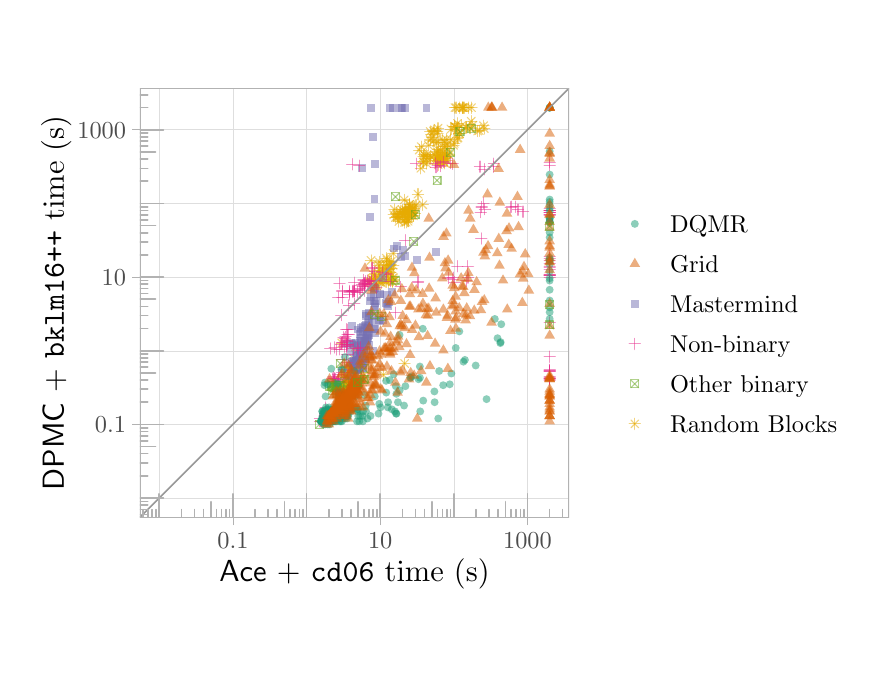
\begin{tikzpicture}[x=1pt,y=1pt]
\definecolor{fillColor}{RGB}{255,255,255}
\path[use as bounding box,fill=fillColor,fill opacity=0.00] (0,0) rectangle (303.53,224.04);
\begin{scope}
\path[clip] (  0.00, 16.35) rectangle (303.53,207.69);
\definecolor{drawColor}{RGB}{255,255,255}
\definecolor{fillColor}{RGB}{255,255,255}

\path[draw=drawColor,line width= 0.6pt,line join=round,line cap=round,fill=fillColor] (  0.00, 16.35) rectangle (303.53,207.69);
\end{scope}
\begin{scope}
\path[clip] ( 40.51, 47.03) rectangle (195.67,202.19);
\definecolor{fillColor}{RGB}{255,255,255}

\path[fill=fillColor] ( 40.51, 47.03) rectangle (195.67,202.19);
\definecolor{drawColor}{gray}{0.87}

\path[draw=drawColor,line width= 0.1pt,line join=round] ( 40.51, 54.09) --
	(195.67, 54.09);

\path[draw=drawColor,line width= 0.1pt,line join=round] ( 40.51,107.30) --
	(195.67,107.30);

\path[draw=drawColor,line width= 0.1pt,line join=round] ( 40.51,160.52) --
	(195.67,160.52);

\path[draw=drawColor,line width= 0.1pt,line join=round] ( 47.56, 47.03) --
	( 47.56,202.19);

\path[draw=drawColor,line width= 0.1pt,line join=round] (100.78, 47.03) --
	(100.78,202.19);

\path[draw=drawColor,line width= 0.1pt,line join=round] (154.00, 47.03) --
	(154.00,202.19);

\path[draw=drawColor,line width= 0.3pt,line join=round] ( 40.51, 80.69) --
	(195.67, 80.69);

\path[draw=drawColor,line width= 0.3pt,line join=round] ( 40.51,133.91) --
	(195.67,133.91);

\path[draw=drawColor,line width= 0.3pt,line join=round] ( 40.51,187.13) --
	(195.67,187.13);

\path[draw=drawColor,line width= 0.3pt,line join=round] ( 74.17, 47.03) --
	( 74.17,202.19);

\path[draw=drawColor,line width= 0.3pt,line join=round] (127.39, 47.03) --
	(127.39,202.19);

\path[draw=drawColor,line width= 0.3pt,line join=round] (180.61, 47.03) --
	(180.61,202.19);
\definecolor{drawColor}{RGB}{230,171,2}

\path[draw=drawColor,draw opacity=0.50,line width= 0.4pt,line join=round,line cap=round] (114.28, 91.57) -- (117.14, 94.42);

\path[draw=drawColor,draw opacity=0.50,line width= 0.4pt,line join=round,line cap=round] (114.28, 94.42) -- (117.14, 91.57);

\path[draw=drawColor,draw opacity=0.50,line width= 0.4pt,line join=round,line cap=round] (113.69, 93.00) -- (117.73, 93.00);

\path[draw=drawColor,draw opacity=0.50,line width= 0.4pt,line join=round,line cap=round] (115.71, 90.98) -- (115.71, 95.01);

\path[draw=drawColor,draw opacity=0.50,line width= 0.4pt,line join=round,line cap=round] (115.63, 91.57) -- (118.48, 94.42);

\path[draw=drawColor,draw opacity=0.50,line width= 0.4pt,line join=round,line cap=round] (115.63, 94.42) -- (118.48, 91.57);

\path[draw=drawColor,draw opacity=0.50,line width= 0.4pt,line join=round,line cap=round] (115.04, 93.00) -- (119.07, 93.00);

\path[draw=drawColor,draw opacity=0.50,line width= 0.4pt,line join=round,line cap=round] (117.06, 90.98) -- (117.06, 95.01);

\path[draw=drawColor,draw opacity=0.50,line width= 0.4pt,line join=round,line cap=round] (113.83, 93.41) -- (116.68, 96.26);

\path[draw=drawColor,draw opacity=0.50,line width= 0.4pt,line join=round,line cap=round] (113.83, 96.26) -- (116.68, 93.41);

\path[draw=drawColor,draw opacity=0.50,line width= 0.4pt,line join=round,line cap=round] (113.24, 94.84) -- (117.27, 94.84);

\path[draw=drawColor,draw opacity=0.50,line width= 0.4pt,line join=round,line cap=round] (115.26, 92.82) -- (115.26, 96.85);

\path[draw=drawColor,draw opacity=0.50,line width= 0.4pt,line join=round,line cap=round] (116.63, 94.07) -- (119.48, 96.92);

\path[draw=drawColor,draw opacity=0.50,line width= 0.4pt,line join=round,line cap=round] (116.63, 96.92) -- (119.48, 94.07);

\path[draw=drawColor,draw opacity=0.50,line width= 0.4pt,line join=round,line cap=round] (116.04, 95.50) -- (120.08, 95.50);

\path[draw=drawColor,draw opacity=0.50,line width= 0.4pt,line join=round,line cap=round] (118.06, 93.48) -- (118.06, 97.51);

\path[draw=drawColor,draw opacity=0.50,line width= 0.4pt,line join=round,line cap=round] (115.77, 93.06) -- (118.62, 95.92);

\path[draw=drawColor,draw opacity=0.50,line width= 0.4pt,line join=round,line cap=round] (115.77, 95.92) -- (118.62, 93.06);

\path[draw=drawColor,draw opacity=0.50,line width= 0.4pt,line join=round,line cap=round] (115.18, 94.49) -- (119.21, 94.49);

\path[draw=drawColor,draw opacity=0.50,line width= 0.4pt,line join=round,line cap=round] (117.20, 92.47) -- (117.20, 96.51);

\path[draw=drawColor,draw opacity=0.50,line width= 0.4pt,line join=round,line cap=round] (114.41, 91.57) -- (117.26, 94.42);

\path[draw=drawColor,draw opacity=0.50,line width= 0.4pt,line join=round,line cap=round] (114.41, 94.42) -- (117.26, 91.57);

\path[draw=drawColor,draw opacity=0.50,line width= 0.4pt,line join=round,line cap=round] (113.82, 93.00) -- (117.85, 93.00);

\path[draw=drawColor,draw opacity=0.50,line width= 0.4pt,line join=round,line cap=round] (115.84, 90.98) -- (115.84, 95.01);

\path[draw=drawColor,draw opacity=0.50,line width= 0.4pt,line join=round,line cap=round] (110.48, 91.96) -- (113.34, 94.82);

\path[draw=drawColor,draw opacity=0.50,line width= 0.4pt,line join=round,line cap=round] (110.48, 94.82) -- (113.34, 91.96);

\path[draw=drawColor,draw opacity=0.50,line width= 0.4pt,line join=round,line cap=round] (109.89, 93.39) -- (113.93, 93.39);

\path[draw=drawColor,draw opacity=0.50,line width= 0.4pt,line join=round,line cap=round] (111.91, 91.37) -- (111.91, 95.41);

\path[draw=drawColor,draw opacity=0.50,line width= 0.4pt,line join=round,line cap=round] (114.90, 93.74) -- (117.75, 96.60);

\path[draw=drawColor,draw opacity=0.50,line width= 0.4pt,line join=round,line cap=round] (114.90, 96.60) -- (117.75, 93.74);

\path[draw=drawColor,draw opacity=0.50,line width= 0.4pt,line join=round,line cap=round] (114.31, 95.17) -- (118.35, 95.17);

\path[draw=drawColor,draw opacity=0.50,line width= 0.4pt,line join=round,line cap=round] (116.33, 93.15) -- (116.33, 97.19);

\path[draw=drawColor,draw opacity=0.50,line width= 0.4pt,line join=round,line cap=round] (113.86, 94.69) -- (116.72, 97.55);

\path[draw=drawColor,draw opacity=0.50,line width= 0.4pt,line join=round,line cap=round] (113.86, 97.55) -- (116.72, 94.69);

\path[draw=drawColor,draw opacity=0.50,line width= 0.4pt,line join=round,line cap=round] (113.27, 96.12) -- (117.31, 96.12);

\path[draw=drawColor,draw opacity=0.50,line width= 0.4pt,line join=round,line cap=round] (115.29, 94.10) -- (115.29, 98.14);

\path[draw=drawColor,draw opacity=0.50,line width= 0.4pt,line join=round,line cap=round] (112.83, 91.17) -- (115.68, 94.02);

\path[draw=drawColor,draw opacity=0.50,line width= 0.4pt,line join=round,line cap=round] (112.83, 94.02) -- (115.68, 91.17);

\path[draw=drawColor,draw opacity=0.50,line width= 0.4pt,line join=round,line cap=round] (112.24, 92.59) -- (116.27, 92.59);

\path[draw=drawColor,draw opacity=0.50,line width= 0.4pt,line join=round,line cap=round] (114.26, 90.57) -- (114.26, 94.61);

\path[draw=drawColor,draw opacity=0.50,line width= 0.4pt,line join=round,line cap=round] (111.33, 92.34) -- (114.19, 95.19);

\path[draw=drawColor,draw opacity=0.50,line width= 0.4pt,line join=round,line cap=round] (111.33, 95.19) -- (114.19, 92.34);

\path[draw=drawColor,draw opacity=0.50,line width= 0.4pt,line join=round,line cap=round] (110.74, 93.77) -- (114.78, 93.77);

\path[draw=drawColor,draw opacity=0.50,line width= 0.4pt,line join=round,line cap=round] (112.76, 91.75) -- (112.76, 95.79);

\path[draw=drawColor,draw opacity=0.50,line width= 0.4pt,line join=round,line cap=round] (115.88, 91.96) -- (118.73, 94.82);

\path[draw=drawColor,draw opacity=0.50,line width= 0.4pt,line join=round,line cap=round] (115.88, 94.82) -- (118.73, 91.96);

\path[draw=drawColor,draw opacity=0.50,line width= 0.4pt,line join=round,line cap=round] (115.29, 93.39) -- (119.33, 93.39);

\path[draw=drawColor,draw opacity=0.50,line width= 0.4pt,line join=round,line cap=round] (117.31, 91.37) -- (117.31, 95.41);

\path[draw=drawColor,draw opacity=0.50,line width= 0.4pt,line join=round,line cap=round] (114.28, 92.71) -- (117.14, 95.56);

\path[draw=drawColor,draw opacity=0.50,line width= 0.4pt,line join=round,line cap=round] (114.28, 95.56) -- (117.14, 92.71);

\path[draw=drawColor,draw opacity=0.50,line width= 0.4pt,line join=round,line cap=round] (113.69, 94.13) -- (117.73, 94.13);

\path[draw=drawColor,draw opacity=0.50,line width= 0.4pt,line join=round,line cap=round] (115.71, 92.12) -- (115.71, 96.15);

\path[draw=drawColor,draw opacity=0.50,line width= 0.4pt,line join=round,line cap=round] (113.46, 91.96) -- (116.31, 94.82);

\path[draw=drawColor,draw opacity=0.50,line width= 0.4pt,line join=round,line cap=round] (113.46, 94.82) -- (116.31, 91.96);

\path[draw=drawColor,draw opacity=0.50,line width= 0.4pt,line join=round,line cap=round] (112.87, 93.39) -- (116.91, 93.39);

\path[draw=drawColor,draw opacity=0.50,line width= 0.4pt,line join=round,line cap=round] (114.89, 91.37) -- (114.89, 95.41);

\path[draw=drawColor,draw opacity=0.50,line width= 0.4pt,line join=round,line cap=round] (116.32, 93.74) -- (119.17, 96.60);

\path[draw=drawColor,draw opacity=0.50,line width= 0.4pt,line join=round,line cap=round] (116.32, 96.60) -- (119.17, 93.74);

\path[draw=drawColor,draw opacity=0.50,line width= 0.4pt,line join=round,line cap=round] (115.72, 95.17) -- (119.76, 95.17);

\path[draw=drawColor,draw opacity=0.50,line width= 0.4pt,line join=round,line cap=round] (117.74, 93.15) -- (117.74, 97.19);

\path[draw=drawColor,draw opacity=0.50,line width= 0.4pt,line join=round,line cap=round] (116.34, 92.71) -- (119.20, 95.56);

\path[draw=drawColor,draw opacity=0.50,line width= 0.4pt,line join=round,line cap=round] (116.34, 95.56) -- (119.20, 92.71);

\path[draw=drawColor,draw opacity=0.50,line width= 0.4pt,line join=round,line cap=round] (115.75, 94.13) -- (119.79, 94.13);

\path[draw=drawColor,draw opacity=0.50,line width= 0.4pt,line join=round,line cap=round] (117.77, 92.12) -- (117.77, 96.15);

\path[draw=drawColor,draw opacity=0.50,line width= 0.4pt,line join=round,line cap=round] (116.21, 97.15) -- (119.06,100.00);

\path[draw=drawColor,draw opacity=0.50,line width= 0.4pt,line join=round,line cap=round] (116.21,100.00) -- (119.06, 97.15);

\path[draw=drawColor,draw opacity=0.50,line width= 0.4pt,line join=round,line cap=round] (115.62, 98.58) -- (119.65, 98.58);

\path[draw=drawColor,draw opacity=0.50,line width= 0.4pt,line join=round,line cap=round] (117.64, 96.56) -- (117.64,100.59);

\path[draw=drawColor,draw opacity=0.50,line width= 0.4pt,line join=round,line cap=round] (116.86, 95.57) -- (119.72, 98.43);

\path[draw=drawColor,draw opacity=0.50,line width= 0.4pt,line join=round,line cap=round] (116.86, 98.43) -- (119.72, 95.57);

\path[draw=drawColor,draw opacity=0.50,line width= 0.4pt,line join=round,line cap=round] (116.27, 97.00) -- (120.31, 97.00);

\path[draw=drawColor,draw opacity=0.50,line width= 0.4pt,line join=round,line cap=round] (118.29, 94.98) -- (118.29, 99.02);

\path[draw=drawColor,draw opacity=0.50,line width= 0.4pt,line join=round,line cap=round] (113.70, 94.39) -- (116.55, 97.24);

\path[draw=drawColor,draw opacity=0.50,line width= 0.4pt,line join=round,line cap=round] (113.70, 97.24) -- (116.55, 94.39);

\path[draw=drawColor,draw opacity=0.50,line width= 0.4pt,line join=round,line cap=round] (113.11, 95.81) -- (117.14, 95.81);

\path[draw=drawColor,draw opacity=0.50,line width= 0.4pt,line join=round,line cap=round] (115.12, 93.80) -- (115.12, 97.83);

\path[draw=drawColor,draw opacity=0.50,line width= 0.4pt,line join=round,line cap=round] (117.50, 94.99) -- (120.36, 97.85);

\path[draw=drawColor,draw opacity=0.50,line width= 0.4pt,line join=round,line cap=round] (117.50, 97.85) -- (120.36, 94.99);

\path[draw=drawColor,draw opacity=0.50,line width= 0.4pt,line join=round,line cap=round] (116.91, 96.42) -- (120.95, 96.42);

\path[draw=drawColor,draw opacity=0.50,line width= 0.4pt,line join=round,line cap=round] (118.93, 94.40) -- (118.93, 98.44);

\path[draw=drawColor,draw opacity=0.50,line width= 0.4pt,line join=round,line cap=round] (114.28, 96.65) -- (117.14, 99.50);

\path[draw=drawColor,draw opacity=0.50,line width= 0.4pt,line join=round,line cap=round] (114.28, 99.50) -- (117.14, 96.65);

\path[draw=drawColor,draw opacity=0.50,line width= 0.4pt,line join=round,line cap=round] (113.69, 98.07) -- (117.73, 98.07);

\path[draw=drawColor,draw opacity=0.50,line width= 0.4pt,line join=round,line cap=round] (115.71, 96.06) -- (115.71,100.09);

\path[draw=drawColor,draw opacity=0.50,line width= 0.4pt,line join=round,line cap=round] (114.28, 93.74) -- (117.14, 96.60);

\path[draw=drawColor,draw opacity=0.50,line width= 0.4pt,line join=round,line cap=round] (114.28, 96.60) -- (117.14, 93.74);

\path[draw=drawColor,draw opacity=0.50,line width= 0.4pt,line join=round,line cap=round] (113.69, 95.17) -- (117.73, 95.17);

\path[draw=drawColor,draw opacity=0.50,line width= 0.4pt,line join=round,line cap=round] (115.71, 93.15) -- (115.71, 97.19);

\path[draw=drawColor,draw opacity=0.50,line width= 0.4pt,line join=round,line cap=round] (112.09,108.64) -- (114.94,111.49);

\path[draw=drawColor,draw opacity=0.50,line width= 0.4pt,line join=round,line cap=round] (112.09,111.49) -- (114.94,108.64);

\path[draw=drawColor,draw opacity=0.50,line width= 0.4pt,line join=round,line cap=round] (111.50,110.06) -- (115.53,110.06);

\path[draw=drawColor,draw opacity=0.50,line width= 0.4pt,line join=round,line cap=round] (113.51,108.05) -- (113.51,112.08);

\path[draw=drawColor,draw opacity=0.50,line width= 0.4pt,line join=round,line cap=round] (113.76, 93.74) -- (116.62, 96.60);

\path[draw=drawColor,draw opacity=0.50,line width= 0.4pt,line join=round,line cap=round] (113.76, 96.60) -- (116.62, 93.74);

\path[draw=drawColor,draw opacity=0.50,line width= 0.4pt,line join=round,line cap=round] (113.17, 95.17) -- (117.21, 95.17);

\path[draw=drawColor,draw opacity=0.50,line width= 0.4pt,line join=round,line cap=round] (115.19, 93.15) -- (115.19, 97.19);

\path[draw=drawColor,draw opacity=0.50,line width= 0.4pt,line join=round,line cap=round] (113.29, 93.74) -- (116.14, 96.60);

\path[draw=drawColor,draw opacity=0.50,line width= 0.4pt,line join=round,line cap=round] (113.29, 96.60) -- (116.14, 93.74);

\path[draw=drawColor,draw opacity=0.50,line width= 0.4pt,line join=round,line cap=round] (112.70, 95.17) -- (116.73, 95.17);

\path[draw=drawColor,draw opacity=0.50,line width= 0.4pt,line join=round,line cap=round] (114.72, 93.15) -- (114.72, 97.19);

\path[draw=drawColor,draw opacity=0.50,line width= 0.4pt,line join=round,line cap=round] (116.21, 95.57) -- (119.06, 98.43);

\path[draw=drawColor,draw opacity=0.50,line width= 0.4pt,line join=round,line cap=round] (116.21, 98.43) -- (119.06, 95.57);

\path[draw=drawColor,draw opacity=0.50,line width= 0.4pt,line join=round,line cap=round] (115.62, 97.00) -- (119.65, 97.00);

\path[draw=drawColor,draw opacity=0.50,line width= 0.4pt,line join=round,line cap=round] (117.64, 94.98) -- (117.64, 99.02);

\path[draw=drawColor,draw opacity=0.50,line width= 0.4pt,line join=round,line cap=round] (117.01, 98.09) -- (119.87,100.95);

\path[draw=drawColor,draw opacity=0.50,line width= 0.4pt,line join=round,line cap=round] (117.01,100.95) -- (119.87, 98.09);

\path[draw=drawColor,draw opacity=0.50,line width= 0.4pt,line join=round,line cap=round] (116.42, 99.52) -- (120.46, 99.52);

\path[draw=drawColor,draw opacity=0.50,line width= 0.4pt,line join=round,line cap=round] (118.44, 97.50) -- (118.44,101.54);

\path[draw=drawColor,draw opacity=0.50,line width= 0.4pt,line join=round,line cap=round] (115.69, 94.69) -- (118.54, 97.55);

\path[draw=drawColor,draw opacity=0.50,line width= 0.4pt,line join=round,line cap=round] (115.69, 97.55) -- (118.54, 94.69);

\path[draw=drawColor,draw opacity=0.50,line width= 0.4pt,line join=round,line cap=round] (115.10, 96.12) -- (119.13, 96.12);

\path[draw=drawColor,draw opacity=0.50,line width= 0.4pt,line join=round,line cap=round] (117.11, 94.10) -- (117.11, 98.14);

\path[draw=drawColor,draw opacity=0.50,line width= 0.4pt,line join=round,line cap=round] (113.01, 93.06) -- (115.86, 95.92);

\path[draw=drawColor,draw opacity=0.50,line width= 0.4pt,line join=round,line cap=round] (113.01, 95.92) -- (115.86, 93.06);

\path[draw=drawColor,draw opacity=0.50,line width= 0.4pt,line join=round,line cap=round] (112.42, 94.49) -- (116.45, 94.49);

\path[draw=drawColor,draw opacity=0.50,line width= 0.4pt,line join=round,line cap=round] (114.44, 92.47) -- (114.44, 96.51);

\path[draw=drawColor,draw opacity=0.50,line width= 0.4pt,line join=round,line cap=round] (114.31, 95.29) -- (117.17, 98.14);

\path[draw=drawColor,draw opacity=0.50,line width= 0.4pt,line join=round,line cap=round] (114.31, 98.14) -- (117.17, 95.29);

\path[draw=drawColor,draw opacity=0.50,line width= 0.4pt,line join=round,line cap=round] (113.72, 96.71) -- (117.76, 96.71);

\path[draw=drawColor,draw opacity=0.50,line width= 0.4pt,line join=round,line cap=round] (115.74, 94.70) -- (115.74, 98.73);

\path[draw=drawColor,draw opacity=0.50,line width= 0.4pt,line join=round,line cap=round] (112.90, 93.06) -- (115.76, 95.92);

\path[draw=drawColor,draw opacity=0.50,line width= 0.4pt,line join=round,line cap=round] (112.90, 95.92) -- (115.76, 93.06);

\path[draw=drawColor,draw opacity=0.50,line width= 0.4pt,line join=round,line cap=round] (112.31, 94.49) -- (116.35, 94.49);

\path[draw=drawColor,draw opacity=0.50,line width= 0.4pt,line join=round,line cap=round] (114.33, 92.47) -- (114.33, 96.51);

\path[draw=drawColor,draw opacity=0.50,line width= 0.4pt,line join=round,line cap=round] (114.63, 97.39) -- (117.48,100.25);

\path[draw=drawColor,draw opacity=0.50,line width= 0.4pt,line join=round,line cap=round] (114.63,100.25) -- (117.48, 97.39);

\path[draw=drawColor,draw opacity=0.50,line width= 0.4pt,line join=round,line cap=round] (114.04, 98.82) -- (118.07, 98.82);

\path[draw=drawColor,draw opacity=0.50,line width= 0.4pt,line join=round,line cap=round] (116.05, 96.80) -- (116.05,100.84);

\path[draw=drawColor,draw opacity=0.50,line width= 0.4pt,line join=round,line cap=round] (117.86,106.33) -- (120.71,109.18);

\path[draw=drawColor,draw opacity=0.50,line width= 0.4pt,line join=round,line cap=round] (117.86,109.18) -- (120.71,106.33);

\path[draw=drawColor,draw opacity=0.50,line width= 0.4pt,line join=round,line cap=round] (117.27,107.76) -- (121.30,107.76);

\path[draw=drawColor,draw opacity=0.50,line width= 0.4pt,line join=round,line cap=round] (119.29,105.74) -- (119.29,109.77);

\path[draw=drawColor,draw opacity=0.50,line width= 0.4pt,line join=round,line cap=round] (114.06, 97.15) -- (116.91,100.00);

\path[draw=drawColor,draw opacity=0.50,line width= 0.4pt,line join=round,line cap=round] (114.06,100.00) -- (116.91, 97.15);

\path[draw=drawColor,draw opacity=0.50,line width= 0.4pt,line join=round,line cap=round] (113.47, 98.58) -- (117.50, 98.58);

\path[draw=drawColor,draw opacity=0.50,line width= 0.4pt,line join=round,line cap=round] (115.49, 96.56) -- (115.49,100.59);

\path[draw=drawColor,draw opacity=0.50,line width= 0.4pt,line join=round,line cap=round] (113.73, 96.12) -- (116.58, 98.98);

\path[draw=drawColor,draw opacity=0.50,line width= 0.4pt,line join=round,line cap=round] (113.73, 98.98) -- (116.58, 96.12);

\path[draw=drawColor,draw opacity=0.50,line width= 0.4pt,line join=round,line cap=round] (113.14, 97.55) -- (117.17, 97.55);

\path[draw=drawColor,draw opacity=0.50,line width= 0.4pt,line join=round,line cap=round] (115.16, 95.53) -- (115.16, 99.57);

\path[draw=drawColor,draw opacity=0.50,line width= 0.4pt,line join=round,line cap=round] (115.49, 96.90) -- (118.34, 99.76);

\path[draw=drawColor,draw opacity=0.50,line width= 0.4pt,line join=round,line cap=round] (115.49, 99.76) -- (118.34, 96.90);

\path[draw=drawColor,draw opacity=0.50,line width= 0.4pt,line join=round,line cap=round] (114.90, 98.33) -- (118.93, 98.33);

\path[draw=drawColor,draw opacity=0.50,line width= 0.4pt,line join=round,line cap=round] (116.91, 96.31) -- (116.91,100.35);

\path[draw=drawColor,draw opacity=0.50,line width= 0.4pt,line join=round,line cap=round] (117.72, 98.54) -- (120.57,101.39);

\path[draw=drawColor,draw opacity=0.50,line width= 0.4pt,line join=round,line cap=round] (117.72,101.39) -- (120.57, 98.54);

\path[draw=drawColor,draw opacity=0.50,line width= 0.4pt,line join=round,line cap=round] (117.13, 99.97) -- (121.16, 99.97);

\path[draw=drawColor,draw opacity=0.50,line width= 0.4pt,line join=round,line cap=round] (119.14, 97.95) -- (119.14,101.98);

\path[draw=drawColor,draw opacity=0.50,line width= 0.4pt,line join=round,line cap=round] (114.41, 95.29) -- (117.26, 98.14);

\path[draw=drawColor,draw opacity=0.50,line width= 0.4pt,line join=round,line cap=round] (114.41, 98.14) -- (117.26, 95.29);

\path[draw=drawColor,draw opacity=0.50,line width= 0.4pt,line join=round,line cap=round] (113.82, 96.71) -- (117.85, 96.71);

\path[draw=drawColor,draw opacity=0.50,line width= 0.4pt,line join=round,line cap=round] (115.84, 94.70) -- (115.84, 98.73);

\path[draw=drawColor,draw opacity=0.50,line width= 0.4pt,line join=round,line cap=round] (116.42,103.00) -- (119.28,105.86);

\path[draw=drawColor,draw opacity=0.50,line width= 0.4pt,line join=round,line cap=round] (116.42,105.86) -- (119.28,103.00);

\path[draw=drawColor,draw opacity=0.50,line width= 0.4pt,line join=round,line cap=round] (115.83,104.43) -- (119.87,104.43);

\path[draw=drawColor,draw opacity=0.50,line width= 0.4pt,line join=round,line cap=round] (117.85,102.41) -- (117.85,106.45);

\path[draw=drawColor,draw opacity=0.50,line width= 0.4pt,line join=round,line cap=round] (116.13, 99.38) -- (118.98,102.23);

\path[draw=drawColor,draw opacity=0.50,line width= 0.4pt,line join=round,line cap=round] (116.13,102.23) -- (118.98, 99.38);

\path[draw=drawColor,draw opacity=0.50,line width= 0.4pt,line join=round,line cap=round] (115.54,100.81) -- (119.57,100.81);

\path[draw=drawColor,draw opacity=0.50,line width= 0.4pt,line join=round,line cap=round] (117.55, 98.79) -- (117.55,102.82);

\path[draw=drawColor,draw opacity=0.50,line width= 0.4pt,line join=round,line cap=round] (117.36, 97.63) -- (120.21,100.49);

\path[draw=drawColor,draw opacity=0.50,line width= 0.4pt,line join=round,line cap=round] (117.36,100.49) -- (120.21, 97.63);

\path[draw=drawColor,draw opacity=0.50,line width= 0.4pt,line join=round,line cap=round] (116.77, 99.06) -- (120.80, 99.06);

\path[draw=drawColor,draw opacity=0.50,line width= 0.4pt,line join=round,line cap=round] (118.79, 97.04) -- (118.79,101.08);

\path[draw=drawColor,draw opacity=0.50,line width= 0.4pt,line join=round,line cap=round] (116.99,107.19) -- (119.84,110.04);

\path[draw=drawColor,draw opacity=0.50,line width= 0.4pt,line join=round,line cap=round] (116.99,110.04) -- (119.84,107.19);

\path[draw=drawColor,draw opacity=0.50,line width= 0.4pt,line join=round,line cap=round] (116.40,108.61) -- (120.43,108.61);

\path[draw=drawColor,draw opacity=0.50,line width= 0.4pt,line join=round,line cap=round] (118.41,106.59) -- (118.41,110.63);

\path[draw=drawColor,draw opacity=0.50,line width= 0.4pt,line join=round,line cap=round] (127.17, 97.15) -- (130.02,100.00);

\path[draw=drawColor,draw opacity=0.50,line width= 0.4pt,line join=round,line cap=round] (127.17,100.00) -- (130.02, 97.15);

\path[draw=drawColor,draw opacity=0.50,line width= 0.4pt,line join=round,line cap=round] (126.58, 98.58) -- (130.61, 98.58);

\path[draw=drawColor,draw opacity=0.50,line width= 0.4pt,line join=round,line cap=round] (128.59, 96.56) -- (128.59,100.59);

\path[draw=drawColor,draw opacity=0.50,line width= 0.4pt,line join=round,line cap=round] (114.53, 96.12) -- (117.39, 98.98);

\path[draw=drawColor,draw opacity=0.50,line width= 0.4pt,line join=round,line cap=round] (114.53, 98.98) -- (117.39, 96.12);

\path[draw=drawColor,draw opacity=0.50,line width= 0.4pt,line join=round,line cap=round] (113.94, 97.55) -- (117.98, 97.55);

\path[draw=drawColor,draw opacity=0.50,line width= 0.4pt,line join=round,line cap=round] (115.96, 95.53) -- (115.96, 99.57);

\path[draw=drawColor,draw opacity=0.50,line width= 0.4pt,line join=round,line cap=round] (113.25, 95.57) -- (116.11, 98.43);

\path[draw=drawColor,draw opacity=0.50,line width= 0.4pt,line join=round,line cap=round] (113.25, 98.43) -- (116.11, 95.57);

\path[draw=drawColor,draw opacity=0.50,line width= 0.4pt,line join=round,line cap=round] (112.66, 97.00) -- (116.70, 97.00);

\path[draw=drawColor,draw opacity=0.50,line width= 0.4pt,line join=round,line cap=round] (114.68, 94.98) -- (114.68, 99.02);

\path[draw=drawColor,draw opacity=0.50,line width= 0.4pt,line join=round,line cap=round] (119.90, 96.90) -- (122.76, 99.76);

\path[draw=drawColor,draw opacity=0.50,line width= 0.4pt,line join=round,line cap=round] (119.90, 99.76) -- (122.76, 96.90);

\path[draw=drawColor,draw opacity=0.50,line width= 0.4pt,line join=round,line cap=round] (119.31, 98.33) -- (123.35, 98.33);

\path[draw=drawColor,draw opacity=0.50,line width= 0.4pt,line join=round,line cap=round] (121.33, 96.31) -- (121.33,100.35);

\path[draw=drawColor,draw opacity=0.50,line width= 0.4pt,line join=round,line cap=round] (114.53, 96.90) -- (117.39, 99.76);

\path[draw=drawColor,draw opacity=0.50,line width= 0.4pt,line join=round,line cap=round] (114.53, 99.76) -- (117.39, 96.90);

\path[draw=drawColor,draw opacity=0.50,line width= 0.4pt,line join=round,line cap=round] (113.94, 98.33) -- (117.98, 98.33);

\path[draw=drawColor,draw opacity=0.50,line width= 0.4pt,line join=round,line cap=round] (115.96, 96.31) -- (115.96,100.35);

\path[draw=drawColor,draw opacity=0.50,line width= 0.4pt,line join=round,line cap=round] (118.40,100.16) -- (121.26,103.02);

\path[draw=drawColor,draw opacity=0.50,line width= 0.4pt,line join=round,line cap=round] (118.40,103.02) -- (121.26,100.16);

\path[draw=drawColor,draw opacity=0.50,line width= 0.4pt,line join=round,line cap=round] (117.81,101.59) -- (121.85,101.59);

\path[draw=drawColor,draw opacity=0.50,line width= 0.4pt,line join=round,line cap=round] (119.83, 99.57) -- (119.83,103.61);

\path[draw=drawColor,draw opacity=0.50,line width= 0.4pt,line join=round,line cap=round] (128.21,130.78) -- (131.07,133.63);

\path[draw=drawColor,draw opacity=0.50,line width= 0.4pt,line join=round,line cap=round] (128.21,133.63) -- (131.07,130.78);

\path[draw=drawColor,draw opacity=0.50,line width= 0.4pt,line join=round,line cap=round] (127.62,132.21) -- (131.66,132.21);

\path[draw=drawColor,draw opacity=0.50,line width= 0.4pt,line join=round,line cap=round] (129.64,130.19) -- (129.64,134.23);

\path[draw=drawColor,draw opacity=0.50,line width= 0.4pt,line join=round,line cap=round] (126.91,132.43) -- (129.77,135.28);

\path[draw=drawColor,draw opacity=0.50,line width= 0.4pt,line join=round,line cap=round] (126.91,135.28) -- (129.77,132.43);

\path[draw=drawColor,draw opacity=0.50,line width= 0.4pt,line join=round,line cap=round] (126.32,133.85) -- (130.36,133.85);

\path[draw=drawColor,draw opacity=0.50,line width= 0.4pt,line join=round,line cap=round] (128.34,131.84) -- (128.34,135.87);

\path[draw=drawColor,draw opacity=0.50,line width= 0.4pt,line join=round,line cap=round] (122.31,130.82) -- (125.16,133.67);

\path[draw=drawColor,draw opacity=0.50,line width= 0.4pt,line join=round,line cap=round] (122.31,133.67) -- (125.16,130.82);

\path[draw=drawColor,draw opacity=0.50,line width= 0.4pt,line join=round,line cap=round] (121.72,132.25) -- (125.75,132.25);

\path[draw=drawColor,draw opacity=0.50,line width= 0.4pt,line join=round,line cap=round] (123.74,130.23) -- (123.74,134.27);

\path[draw=drawColor,draw opacity=0.50,line width= 0.4pt,line join=round,line cap=round] (126.51,130.29) -- (129.37,133.14);

\path[draw=drawColor,draw opacity=0.50,line width= 0.4pt,line join=round,line cap=round] (126.51,133.14) -- (129.37,130.29);

\path[draw=drawColor,draw opacity=0.50,line width= 0.4pt,line join=round,line cap=round] (125.92,131.72) -- (129.96,131.72);

\path[draw=drawColor,draw opacity=0.50,line width= 0.4pt,line join=round,line cap=round] (127.94,129.70) -- (127.94,133.73);

\path[draw=drawColor,draw opacity=0.50,line width= 0.4pt,line join=round,line cap=round] (130.30,130.89) -- (133.16,133.74);

\path[draw=drawColor,draw opacity=0.50,line width= 0.4pt,line join=round,line cap=round] (130.30,133.74) -- (133.16,130.89);

\path[draw=drawColor,draw opacity=0.50,line width= 0.4pt,line join=round,line cap=round] (129.71,132.31) -- (133.75,132.31);

\path[draw=drawColor,draw opacity=0.50,line width= 0.4pt,line join=round,line cap=round] (131.73,130.30) -- (131.73,134.33);

\path[draw=drawColor,draw opacity=0.50,line width= 0.4pt,line join=round,line cap=round] (130.51,130.85) -- (133.36,133.70);

\path[draw=drawColor,draw opacity=0.50,line width= 0.4pt,line join=round,line cap=round] (130.51,133.70) -- (133.36,130.85);

\path[draw=drawColor,draw opacity=0.50,line width= 0.4pt,line join=round,line cap=round] (129.92,132.27) -- (133.95,132.27);

\path[draw=drawColor,draw opacity=0.50,line width= 0.4pt,line join=round,line cap=round] (131.93,130.26) -- (131.93,134.29);

\path[draw=drawColor,draw opacity=0.50,line width= 0.4pt,line join=round,line cap=round] (123.00,131.79) -- (125.85,134.65);

\path[draw=drawColor,draw opacity=0.50,line width= 0.4pt,line join=round,line cap=round] (123.00,134.65) -- (125.85,131.79);

\path[draw=drawColor,draw opacity=0.50,line width= 0.4pt,line join=round,line cap=round] (122.41,133.22) -- (126.45,133.22);

\path[draw=drawColor,draw opacity=0.50,line width= 0.4pt,line join=round,line cap=round] (124.43,131.20) -- (124.43,135.24);

\path[draw=drawColor,draw opacity=0.50,line width= 0.4pt,line join=round,line cap=round] (124.00,130.87) -- (126.85,133.73);

\path[draw=drawColor,draw opacity=0.50,line width= 0.4pt,line join=round,line cap=round] (124.00,133.73) -- (126.85,130.87);

\path[draw=drawColor,draw opacity=0.50,line width= 0.4pt,line join=round,line cap=round] (123.41,132.30) -- (127.45,132.30);

\path[draw=drawColor,draw opacity=0.50,line width= 0.4pt,line join=round,line cap=round] (125.43,130.28) -- (125.43,134.32);

\path[draw=drawColor,draw opacity=0.50,line width= 0.4pt,line join=round,line cap=round] (123.99,130.87) -- (126.84,133.73);

\path[draw=drawColor,draw opacity=0.50,line width= 0.4pt,line join=round,line cap=round] (123.99,133.73) -- (126.84,130.87);

\path[draw=drawColor,draw opacity=0.50,line width= 0.4pt,line join=round,line cap=round] (123.40,132.30) -- (127.43,132.30);

\path[draw=drawColor,draw opacity=0.50,line width= 0.4pt,line join=round,line cap=round] (125.41,130.28) -- (125.41,134.32);

\path[draw=drawColor,draw opacity=0.50,line width= 0.4pt,line join=round,line cap=round] (123.45,131.27) -- (126.31,134.12);

\path[draw=drawColor,draw opacity=0.50,line width= 0.4pt,line join=round,line cap=round] (123.45,134.12) -- (126.31,131.27);

\path[draw=drawColor,draw opacity=0.50,line width= 0.4pt,line join=round,line cap=round] (122.86,132.69) -- (126.90,132.69);

\path[draw=drawColor,draw opacity=0.50,line width= 0.4pt,line join=round,line cap=round] (124.88,130.68) -- (124.88,134.71);

\path[draw=drawColor,draw opacity=0.50,line width= 0.4pt,line join=round,line cap=round] (121.64,130.19) -- (124.49,133.04);

\path[draw=drawColor,draw opacity=0.50,line width= 0.4pt,line join=round,line cap=round] (121.64,133.04) -- (124.49,130.19);

\path[draw=drawColor,draw opacity=0.50,line width= 0.4pt,line join=round,line cap=round] (121.05,131.62) -- (125.08,131.62);

\path[draw=drawColor,draw opacity=0.50,line width= 0.4pt,line join=round,line cap=round] (123.07,129.60) -- (123.07,133.63);

\path[draw=drawColor,draw opacity=0.50,line width= 0.4pt,line join=round,line cap=round] (128.90,130.70) -- (131.75,133.55);

\path[draw=drawColor,draw opacity=0.50,line width= 0.4pt,line join=round,line cap=round] (128.90,133.55) -- (131.75,130.70);

\path[draw=drawColor,draw opacity=0.50,line width= 0.4pt,line join=round,line cap=round] (128.30,132.13) -- (132.34,132.13);

\path[draw=drawColor,draw opacity=0.50,line width= 0.4pt,line join=round,line cap=round] (130.32,130.11) -- (130.32,134.14);

\path[draw=drawColor,draw opacity=0.50,line width= 0.4pt,line join=round,line cap=round] (130.80,132.26) -- (133.65,135.12);

\path[draw=drawColor,draw opacity=0.50,line width= 0.4pt,line join=round,line cap=round] (130.80,135.12) -- (133.65,132.26);

\path[draw=drawColor,draw opacity=0.50,line width= 0.4pt,line join=round,line cap=round] (130.21,133.69) -- (134.24,133.69);

\path[draw=drawColor,draw opacity=0.50,line width= 0.4pt,line join=round,line cap=round] (132.23,131.67) -- (132.23,135.71);

\path[draw=drawColor,draw opacity=0.50,line width= 0.4pt,line join=round,line cap=round] (128.80,131.73) -- (131.65,134.59);

\path[draw=drawColor,draw opacity=0.50,line width= 0.4pt,line join=round,line cap=round] (128.80,134.59) -- (131.65,131.73);

\path[draw=drawColor,draw opacity=0.50,line width= 0.4pt,line join=round,line cap=round] (128.21,133.16) -- (132.24,133.16);

\path[draw=drawColor,draw opacity=0.50,line width= 0.4pt,line join=round,line cap=round] (130.22,131.14) -- (130.22,135.18);

\path[draw=drawColor,draw opacity=0.50,line width= 0.4pt,line join=round,line cap=round] (125.76,130.59) -- (128.62,133.45);

\path[draw=drawColor,draw opacity=0.50,line width= 0.4pt,line join=round,line cap=round] (125.76,133.45) -- (128.62,130.59);

\path[draw=drawColor,draw opacity=0.50,line width= 0.4pt,line join=round,line cap=round] (125.17,132.02) -- (129.21,132.02);

\path[draw=drawColor,draw opacity=0.50,line width= 0.4pt,line join=round,line cap=round] (127.19,130.00) -- (127.19,134.04);

\path[draw=drawColor,draw opacity=0.50,line width= 0.4pt,line join=round,line cap=round] (127.14,134.41) -- (129.99,137.26);

\path[draw=drawColor,draw opacity=0.50,line width= 0.4pt,line join=round,line cap=round] (127.14,137.26) -- (129.99,134.41);

\path[draw=drawColor,draw opacity=0.50,line width= 0.4pt,line join=round,line cap=round] (126.55,135.83) -- (130.58,135.83);

\path[draw=drawColor,draw opacity=0.50,line width= 0.4pt,line join=round,line cap=round] (128.56,133.82) -- (128.56,137.85);

\path[draw=drawColor,draw opacity=0.50,line width= 0.4pt,line join=round,line cap=round] (128.70,134.43) -- (131.55,137.28);

\path[draw=drawColor,draw opacity=0.50,line width= 0.4pt,line join=round,line cap=round] (128.70,137.28) -- (131.55,134.43);

\path[draw=drawColor,draw opacity=0.50,line width= 0.4pt,line join=round,line cap=round] (128.11,135.85) -- (132.14,135.85);

\path[draw=drawColor,draw opacity=0.50,line width= 0.4pt,line join=round,line cap=round] (130.12,133.84) -- (130.12,137.87);

\path[draw=drawColor,draw opacity=0.50,line width= 0.4pt,line join=round,line cap=round] (122.65,138.50) -- (125.51,141.35);

\path[draw=drawColor,draw opacity=0.50,line width= 0.4pt,line join=round,line cap=round] (122.65,141.35) -- (125.51,138.50);

\path[draw=drawColor,draw opacity=0.50,line width= 0.4pt,line join=round,line cap=round] (122.06,139.93) -- (126.10,139.93);

\path[draw=drawColor,draw opacity=0.50,line width= 0.4pt,line join=round,line cap=round] (124.08,137.91) -- (124.08,141.94);

\path[draw=drawColor,draw opacity=0.50,line width= 0.4pt,line join=round,line cap=round] (125.53,134.94) -- (128.38,137.80);

\path[draw=drawColor,draw opacity=0.50,line width= 0.4pt,line join=round,line cap=round] (125.53,137.80) -- (128.38,134.94);

\path[draw=drawColor,draw opacity=0.50,line width= 0.4pt,line join=round,line cap=round] (124.93,136.37) -- (128.97,136.37);

\path[draw=drawColor,draw opacity=0.50,line width= 0.4pt,line join=round,line cap=round] (126.95,134.35) -- (126.95,138.39);

\path[draw=drawColor,draw opacity=0.50,line width= 0.4pt,line join=round,line cap=round] (126.98,131.68) -- (129.83,134.54);

\path[draw=drawColor,draw opacity=0.50,line width= 0.4pt,line join=round,line cap=round] (126.98,134.54) -- (129.83,131.68);

\path[draw=drawColor,draw opacity=0.50,line width= 0.4pt,line join=round,line cap=round] (126.39,133.11) -- (130.42,133.11);

\path[draw=drawColor,draw opacity=0.50,line width= 0.4pt,line join=round,line cap=round] (128.41,131.09) -- (128.41,135.13);

\path[draw=drawColor,draw opacity=0.50,line width= 0.4pt,line join=round,line cap=round] (130.41,132.22) -- (133.26,135.07);

\path[draw=drawColor,draw opacity=0.50,line width= 0.4pt,line join=round,line cap=round] (130.41,135.07) -- (133.26,132.22);

\path[draw=drawColor,draw opacity=0.50,line width= 0.4pt,line join=round,line cap=round] (129.81,133.64) -- (133.85,133.64);

\path[draw=drawColor,draw opacity=0.50,line width= 0.4pt,line join=round,line cap=round] (131.83,131.62) -- (131.83,135.66);

\path[draw=drawColor,draw opacity=0.50,line width= 0.4pt,line join=round,line cap=round] (125.59,131.96) -- (128.44,134.82);

\path[draw=drawColor,draw opacity=0.50,line width= 0.4pt,line join=round,line cap=round] (125.59,134.82) -- (128.44,131.96);

\path[draw=drawColor,draw opacity=0.50,line width= 0.4pt,line join=round,line cap=round] (124.99,133.39) -- (129.03,133.39);

\path[draw=drawColor,draw opacity=0.50,line width= 0.4pt,line join=round,line cap=round] (127.01,131.37) -- (127.01,135.41);

\path[draw=drawColor,draw opacity=0.50,line width= 0.4pt,line join=round,line cap=round] (125.49,131.65) -- (128.34,134.50);

\path[draw=drawColor,draw opacity=0.50,line width= 0.4pt,line join=round,line cap=round] (125.49,134.50) -- (128.34,131.65);

\path[draw=drawColor,draw opacity=0.50,line width= 0.4pt,line join=round,line cap=round] (124.90,133.07) -- (128.93,133.07);

\path[draw=drawColor,draw opacity=0.50,line width= 0.4pt,line join=round,line cap=round] (126.92,131.05) -- (126.92,135.09);

\path[draw=drawColor,draw opacity=0.50,line width= 0.4pt,line join=round,line cap=round] (125.57,133.56) -- (128.43,136.42);

\path[draw=drawColor,draw opacity=0.50,line width= 0.4pt,line join=round,line cap=round] (125.57,136.42) -- (128.43,133.56);

\path[draw=drawColor,draw opacity=0.50,line width= 0.4pt,line join=round,line cap=round] (124.98,134.99) -- (129.02,134.99);

\path[draw=drawColor,draw opacity=0.50,line width= 0.4pt,line join=round,line cap=round] (127.00,132.97) -- (127.00,137.01);

\path[draw=drawColor,draw opacity=0.50,line width= 0.4pt,line join=round,line cap=round] (126.20,131.63) -- (129.06,134.49);

\path[draw=drawColor,draw opacity=0.50,line width= 0.4pt,line join=round,line cap=round] (126.20,134.49) -- (129.06,131.63);

\path[draw=drawColor,draw opacity=0.50,line width= 0.4pt,line join=round,line cap=round] (125.61,133.06) -- (129.65,133.06);

\path[draw=drawColor,draw opacity=0.50,line width= 0.4pt,line join=round,line cap=round] (127.63,131.04) -- (127.63,135.08);

\path[draw=drawColor,draw opacity=0.50,line width= 0.4pt,line join=round,line cap=round] (122.91,131.57) -- (125.76,134.42);

\path[draw=drawColor,draw opacity=0.50,line width= 0.4pt,line join=round,line cap=round] (122.91,134.42) -- (125.76,131.57);

\path[draw=drawColor,draw opacity=0.50,line width= 0.4pt,line join=round,line cap=round] (122.32,133.00) -- (126.36,133.00);

\path[draw=drawColor,draw opacity=0.50,line width= 0.4pt,line join=round,line cap=round] (124.34,130.98) -- (124.34,135.01);

\path[draw=drawColor,draw opacity=0.50,line width= 0.4pt,line join=round,line cap=round] (124.04,133.65) -- (126.90,136.50);

\path[draw=drawColor,draw opacity=0.50,line width= 0.4pt,line join=round,line cap=round] (124.04,136.50) -- (126.90,133.65);

\path[draw=drawColor,draw opacity=0.50,line width= 0.4pt,line join=round,line cap=round] (123.45,135.07) -- (127.49,135.07);

\path[draw=drawColor,draw opacity=0.50,line width= 0.4pt,line join=round,line cap=round] (125.47,133.06) -- (125.47,137.09);

\path[draw=drawColor,draw opacity=0.50,line width= 0.4pt,line join=round,line cap=round] (130.87,131.44) -- (133.72,134.30);

\path[draw=drawColor,draw opacity=0.50,line width= 0.4pt,line join=round,line cap=round] (130.87,134.30) -- (133.72,131.44);

\path[draw=drawColor,draw opacity=0.50,line width= 0.4pt,line join=round,line cap=round] (130.28,132.87) -- (134.31,132.87);

\path[draw=drawColor,draw opacity=0.50,line width= 0.4pt,line join=round,line cap=round] (132.30,130.85) -- (132.30,134.89);

\path[draw=drawColor,draw opacity=0.50,line width= 0.4pt,line join=round,line cap=round] (126.80,134.90) -- (129.65,137.75);

\path[draw=drawColor,draw opacity=0.50,line width= 0.4pt,line join=round,line cap=round] (126.80,137.75) -- (129.65,134.90);

\path[draw=drawColor,draw opacity=0.50,line width= 0.4pt,line join=round,line cap=round] (126.21,136.32) -- (130.24,136.32);

\path[draw=drawColor,draw opacity=0.50,line width= 0.4pt,line join=round,line cap=round] (128.22,134.30) -- (128.22,138.34);

\path[draw=drawColor,draw opacity=0.50,line width= 0.4pt,line join=round,line cap=round] (126.77,132.60) -- (129.62,135.45);

\path[draw=drawColor,draw opacity=0.50,line width= 0.4pt,line join=round,line cap=round] (126.77,135.45) -- (129.62,132.60);

\path[draw=drawColor,draw opacity=0.50,line width= 0.4pt,line join=round,line cap=round] (126.17,134.03) -- (130.21,134.03);

\path[draw=drawColor,draw opacity=0.50,line width= 0.4pt,line join=round,line cap=round] (128.19,132.01) -- (128.19,136.04);

\path[draw=drawColor,draw opacity=0.50,line width= 0.4pt,line join=round,line cap=round] (129.84,132.71) -- (132.69,135.57);

\path[draw=drawColor,draw opacity=0.50,line width= 0.4pt,line join=round,line cap=round] (129.84,135.57) -- (132.69,132.71);

\path[draw=drawColor,draw opacity=0.50,line width= 0.4pt,line join=round,line cap=round] (129.25,134.14) -- (133.29,134.14);

\path[draw=drawColor,draw opacity=0.50,line width= 0.4pt,line join=round,line cap=round] (131.27,132.12) -- (131.27,136.16);

\path[draw=drawColor,draw opacity=0.50,line width= 0.4pt,line join=round,line cap=round] (129.64,134.10) -- (132.49,136.95);

\path[draw=drawColor,draw opacity=0.50,line width= 0.4pt,line join=round,line cap=round] (129.64,136.95) -- (132.49,134.10);

\path[draw=drawColor,draw opacity=0.50,line width= 0.4pt,line join=round,line cap=round] (129.05,135.53) -- (133.09,135.53);

\path[draw=drawColor,draw opacity=0.50,line width= 0.4pt,line join=round,line cap=round] (131.07,133.51) -- (131.07,137.54);

\path[draw=drawColor,draw opacity=0.50,line width= 0.4pt,line join=round,line cap=round] (128.90,135.14) -- (131.75,137.99);

\path[draw=drawColor,draw opacity=0.50,line width= 0.4pt,line join=round,line cap=round] (128.90,137.99) -- (131.75,135.14);

\path[draw=drawColor,draw opacity=0.50,line width= 0.4pt,line join=round,line cap=round] (128.30,136.56) -- (132.34,136.56);

\path[draw=drawColor,draw opacity=0.50,line width= 0.4pt,line join=round,line cap=round] (130.32,134.55) -- (130.32,138.58);

\path[draw=drawColor,draw opacity=0.50,line width= 0.4pt,line join=round,line cap=round] (128.16,139.31) -- (131.02,142.16);

\path[draw=drawColor,draw opacity=0.50,line width= 0.4pt,line join=round,line cap=round] (128.16,142.16) -- (131.02,139.31);

\path[draw=drawColor,draw opacity=0.50,line width= 0.4pt,line join=round,line cap=round] (127.57,140.74) -- (131.61,140.74);

\path[draw=drawColor,draw opacity=0.50,line width= 0.4pt,line join=round,line cap=round] (129.59,138.72) -- (129.59,142.75);

\path[draw=drawColor,draw opacity=0.50,line width= 0.4pt,line join=round,line cap=round] (130.63,136.71) -- (133.48,139.56);

\path[draw=drawColor,draw opacity=0.50,line width= 0.4pt,line join=round,line cap=round] (130.63,139.56) -- (133.48,136.71);

\path[draw=drawColor,draw opacity=0.50,line width= 0.4pt,line join=round,line cap=round] (130.04,138.13) -- (134.08,138.13);

\path[draw=drawColor,draw opacity=0.50,line width= 0.4pt,line join=round,line cap=round] (132.06,136.11) -- (132.06,140.15);

\path[draw=drawColor,draw opacity=0.50,line width= 0.4pt,line join=round,line cap=round] (130.06,135.54) -- (132.92,138.40);

\path[draw=drawColor,draw opacity=0.50,line width= 0.4pt,line join=round,line cap=round] (130.06,138.40) -- (132.92,135.54);

\path[draw=drawColor,draw opacity=0.50,line width= 0.4pt,line join=round,line cap=round] (129.47,136.97) -- (133.51,136.97);

\path[draw=drawColor,draw opacity=0.50,line width= 0.4pt,line join=round,line cap=round] (131.49,134.95) -- (131.49,138.99);

\path[draw=drawColor,draw opacity=0.50,line width= 0.4pt,line join=round,line cap=round] (129.20,136.83) -- (132.06,139.68);

\path[draw=drawColor,draw opacity=0.50,line width= 0.4pt,line join=round,line cap=round] (129.20,139.68) -- (132.06,136.83);

\path[draw=drawColor,draw opacity=0.50,line width= 0.4pt,line join=round,line cap=round] (128.61,138.25) -- (132.65,138.25);

\path[draw=drawColor,draw opacity=0.50,line width= 0.4pt,line join=round,line cap=round] (130.63,136.23) -- (130.63,140.27);

\path[draw=drawColor,draw opacity=0.50,line width= 0.4pt,line join=round,line cap=round] (128.18,137.00) -- (131.04,139.85);

\path[draw=drawColor,draw opacity=0.50,line width= 0.4pt,line join=round,line cap=round] (128.18,139.85) -- (131.04,137.00);

\path[draw=drawColor,draw opacity=0.50,line width= 0.4pt,line join=round,line cap=round] (127.59,138.43) -- (131.63,138.43);

\path[draw=drawColor,draw opacity=0.50,line width= 0.4pt,line join=round,line cap=round] (129.61,136.41) -- (129.61,140.44);

\path[draw=drawColor,draw opacity=0.50,line width= 0.4pt,line join=round,line cap=round] (129.95,138.11) -- (132.80,140.96);

\path[draw=drawColor,draw opacity=0.50,line width= 0.4pt,line join=round,line cap=round] (129.95,140.96) -- (132.80,138.11);

\path[draw=drawColor,draw opacity=0.50,line width= 0.4pt,line join=round,line cap=round] (129.36,139.54) -- (133.39,139.54);

\path[draw=drawColor,draw opacity=0.50,line width= 0.4pt,line join=round,line cap=round] (131.38,137.52) -- (131.38,141.55);

\path[draw=drawColor,draw opacity=0.50,line width= 0.4pt,line join=round,line cap=round] (125.50,136.69) -- (128.36,139.54);

\path[draw=drawColor,draw opacity=0.50,line width= 0.4pt,line join=round,line cap=round] (125.50,139.54) -- (128.36,136.69);

\path[draw=drawColor,draw opacity=0.50,line width= 0.4pt,line join=round,line cap=round] (124.91,138.12) -- (128.95,138.12);

\path[draw=drawColor,draw opacity=0.50,line width= 0.4pt,line join=round,line cap=round] (126.93,136.10) -- (126.93,140.13);

\path[draw=drawColor,draw opacity=0.50,line width= 0.4pt,line join=round,line cap=round] (125.69,137.93) -- (128.55,140.78);

\path[draw=drawColor,draw opacity=0.50,line width= 0.4pt,line join=round,line cap=round] (125.69,140.78) -- (128.55,137.93);

\path[draw=drawColor,draw opacity=0.50,line width= 0.4pt,line join=round,line cap=round] (125.10,139.36) -- (129.14,139.36);

\path[draw=drawColor,draw opacity=0.50,line width= 0.4pt,line join=round,line cap=round] (127.12,137.34) -- (127.12,141.37);

\path[draw=drawColor,draw opacity=0.50,line width= 0.4pt,line join=round,line cap=round] (127.19,135.75) -- (130.04,138.61);

\path[draw=drawColor,draw opacity=0.50,line width= 0.4pt,line join=round,line cap=round] (127.19,138.61) -- (130.04,135.75);

\path[draw=drawColor,draw opacity=0.50,line width= 0.4pt,line join=round,line cap=round] (126.60,137.18) -- (130.63,137.18);

\path[draw=drawColor,draw opacity=0.50,line width= 0.4pt,line join=round,line cap=round] (128.61,135.16) -- (128.61,139.20);

\path[draw=drawColor,draw opacity=0.50,line width= 0.4pt,line join=round,line cap=round] (123.64,133.34) -- (126.49,136.19);

\path[draw=drawColor,draw opacity=0.50,line width= 0.4pt,line join=round,line cap=round] (123.64,136.19) -- (126.49,133.34);

\path[draw=drawColor,draw opacity=0.50,line width= 0.4pt,line join=round,line cap=round] (123.05,134.77) -- (127.08,134.77);

\path[draw=drawColor,draw opacity=0.50,line width= 0.4pt,line join=round,line cap=round] (125.07,132.75) -- (125.07,136.79);

\path[draw=drawColor,draw opacity=0.50,line width= 0.4pt,line join=round,line cap=round] (129.79,136.97) -- (132.65,139.82);

\path[draw=drawColor,draw opacity=0.50,line width= 0.4pt,line join=round,line cap=round] (129.79,139.82) -- (132.65,136.97);

\path[draw=drawColor,draw opacity=0.50,line width= 0.4pt,line join=round,line cap=round] (129.20,138.39) -- (133.24,138.39);

\path[draw=drawColor,draw opacity=0.50,line width= 0.4pt,line join=round,line cap=round] (131.22,136.38) -- (131.22,140.41);

\path[draw=drawColor,draw opacity=0.50,line width= 0.4pt,line join=round,line cap=round] (129.15,136.87) -- (132.01,139.72);

\path[draw=drawColor,draw opacity=0.50,line width= 0.4pt,line join=round,line cap=round] (129.15,139.72) -- (132.01,136.87);

\path[draw=drawColor,draw opacity=0.50,line width= 0.4pt,line join=round,line cap=round] (128.56,138.29) -- (132.60,138.29);

\path[draw=drawColor,draw opacity=0.50,line width= 0.4pt,line join=round,line cap=round] (130.58,136.27) -- (130.58,140.31);

\path[draw=drawColor,draw opacity=0.50,line width= 0.4pt,line join=round,line cap=round] (129.04,135.08) -- (131.89,137.93);

\path[draw=drawColor,draw opacity=0.50,line width= 0.4pt,line join=round,line cap=round] (129.04,137.93) -- (131.89,135.08);

\path[draw=drawColor,draw opacity=0.50,line width= 0.4pt,line join=round,line cap=round] (128.45,136.51) -- (132.48,136.51);

\path[draw=drawColor,draw opacity=0.50,line width= 0.4pt,line join=round,line cap=round] (130.46,134.49) -- (130.46,138.53);

\path[draw=drawColor,draw opacity=0.50,line width= 0.4pt,line join=round,line cap=round] (128.42,138.62) -- (131.27,141.47);

\path[draw=drawColor,draw opacity=0.50,line width= 0.4pt,line join=round,line cap=round] (128.42,141.47) -- (131.27,138.62);

\path[draw=drawColor,draw opacity=0.50,line width= 0.4pt,line join=round,line cap=round] (127.83,140.04) -- (131.86,140.04);

\path[draw=drawColor,draw opacity=0.50,line width= 0.4pt,line join=round,line cap=round] (129.85,138.02) -- (129.85,142.06);

\path[draw=drawColor,draw opacity=0.50,line width= 0.4pt,line join=round,line cap=round] (130.69,141.02) -- (133.54,143.88);

\path[draw=drawColor,draw opacity=0.50,line width= 0.4pt,line join=round,line cap=round] (130.69,143.88) -- (133.54,141.02);

\path[draw=drawColor,draw opacity=0.50,line width= 0.4pt,line join=round,line cap=round] (130.09,142.45) -- (134.13,142.45);

\path[draw=drawColor,draw opacity=0.50,line width= 0.4pt,line join=round,line cap=round] (132.11,140.43) -- (132.11,144.47);

\path[draw=drawColor,draw opacity=0.50,line width= 0.4pt,line join=round,line cap=round] (134.77,152.24) -- (137.63,155.10);

\path[draw=drawColor,draw opacity=0.50,line width= 0.4pt,line join=round,line cap=round] (134.77,155.10) -- (137.63,152.24);

\path[draw=drawColor,draw opacity=0.50,line width= 0.4pt,line join=round,line cap=round] (134.18,153.67) -- (138.22,153.67);

\path[draw=drawColor,draw opacity=0.50,line width= 0.4pt,line join=round,line cap=round] (136.20,151.65) -- (136.20,155.69);

\path[draw=drawColor,draw opacity=0.50,line width= 0.4pt,line join=round,line cap=round] (134.76,153.17) -- (137.61,156.02);

\path[draw=drawColor,draw opacity=0.50,line width= 0.4pt,line join=round,line cap=round] (134.76,156.02) -- (137.61,153.17);

\path[draw=drawColor,draw opacity=0.50,line width= 0.4pt,line join=round,line cap=round] (134.17,154.60) -- (138.20,154.60);

\path[draw=drawColor,draw opacity=0.50,line width= 0.4pt,line join=round,line cap=round] (136.19,152.58) -- (136.19,156.61);

\path[draw=drawColor,draw opacity=0.50,line width= 0.4pt,line join=round,line cap=round] (136.20,153.43) -- (139.06,156.28);

\path[draw=drawColor,draw opacity=0.50,line width= 0.4pt,line join=round,line cap=round] (136.20,156.28) -- (139.06,153.43);

\path[draw=drawColor,draw opacity=0.50,line width= 0.4pt,line join=round,line cap=round] (135.61,154.85) -- (139.65,154.85);

\path[draw=drawColor,draw opacity=0.50,line width= 0.4pt,line join=round,line cap=round] (137.63,152.83) -- (137.63,156.87);

\path[draw=drawColor,draw opacity=0.50,line width= 0.4pt,line join=round,line cap=round] (136.02,152.69) -- (138.87,155.54);

\path[draw=drawColor,draw opacity=0.50,line width= 0.4pt,line join=round,line cap=round] (136.02,155.54) -- (138.87,152.69);

\path[draw=drawColor,draw opacity=0.50,line width= 0.4pt,line join=round,line cap=round] (135.42,154.12) -- (139.46,154.12);

\path[draw=drawColor,draw opacity=0.50,line width= 0.4pt,line join=round,line cap=round] (137.44,152.10) -- (137.44,156.14);

\path[draw=drawColor,draw opacity=0.50,line width= 0.4pt,line join=round,line cap=round] (134.93,155.89) -- (137.78,158.75);

\path[draw=drawColor,draw opacity=0.50,line width= 0.4pt,line join=round,line cap=round] (134.93,158.75) -- (137.78,155.89);

\path[draw=drawColor,draw opacity=0.50,line width= 0.4pt,line join=round,line cap=round] (134.34,157.32) -- (138.37,157.32);

\path[draw=drawColor,draw opacity=0.50,line width= 0.4pt,line join=round,line cap=round] (136.36,155.30) -- (136.36,159.34);

\path[draw=drawColor,draw opacity=0.50,line width= 0.4pt,line join=round,line cap=round] (135.99,154.48) -- (138.84,157.33);

\path[draw=drawColor,draw opacity=0.50,line width= 0.4pt,line join=round,line cap=round] (135.99,157.33) -- (138.84,154.48);

\path[draw=drawColor,draw opacity=0.50,line width= 0.4pt,line join=round,line cap=round] (135.40,155.91) -- (139.44,155.91);

\path[draw=drawColor,draw opacity=0.50,line width= 0.4pt,line join=round,line cap=round] (137.42,153.89) -- (137.42,157.92);

\path[draw=drawColor,draw opacity=0.50,line width= 0.4pt,line join=round,line cap=round] (132.08,154.01) -- (134.93,156.87);

\path[draw=drawColor,draw opacity=0.50,line width= 0.4pt,line join=round,line cap=round] (132.08,156.87) -- (134.93,154.01);

\path[draw=drawColor,draw opacity=0.50,line width= 0.4pt,line join=round,line cap=round] (131.49,155.44) -- (135.52,155.44);

\path[draw=drawColor,draw opacity=0.50,line width= 0.4pt,line join=round,line cap=round] (133.51,153.42) -- (133.51,157.46);

\path[draw=drawColor,draw opacity=0.50,line width= 0.4pt,line join=round,line cap=round] (130.82,155.04) -- (133.68,157.89);

\path[draw=drawColor,draw opacity=0.50,line width= 0.4pt,line join=round,line cap=round] (130.82,157.89) -- (133.68,155.04);

\path[draw=drawColor,draw opacity=0.50,line width= 0.4pt,line join=round,line cap=round] (130.23,156.47) -- (134.27,156.47);

\path[draw=drawColor,draw opacity=0.50,line width= 0.4pt,line join=round,line cap=round] (132.25,154.45) -- (132.25,158.49);

\path[draw=drawColor,draw opacity=0.50,line width= 0.4pt,line join=round,line cap=round] (132.14,154.48) -- (134.99,157.33);

\path[draw=drawColor,draw opacity=0.50,line width= 0.4pt,line join=round,line cap=round] (132.14,157.33) -- (134.99,154.48);

\path[draw=drawColor,draw opacity=0.50,line width= 0.4pt,line join=round,line cap=round] (131.55,155.91) -- (135.59,155.91);

\path[draw=drawColor,draw opacity=0.50,line width= 0.4pt,line join=round,line cap=round] (133.57,153.89) -- (133.57,157.92);

\path[draw=drawColor,draw opacity=0.50,line width= 0.4pt,line join=round,line cap=round] (134.49,155.12) -- (137.34,157.97);

\path[draw=drawColor,draw opacity=0.50,line width= 0.4pt,line join=round,line cap=round] (134.49,157.97) -- (137.34,155.12);

\path[draw=drawColor,draw opacity=0.50,line width= 0.4pt,line join=round,line cap=round] (133.90,156.55) -- (137.94,156.55);

\path[draw=drawColor,draw opacity=0.50,line width= 0.4pt,line join=round,line cap=round] (135.92,154.53) -- (135.92,158.56);

\path[draw=drawColor,draw opacity=0.50,line width= 0.4pt,line join=round,line cap=round] (134.73,156.09) -- (137.59,158.94);

\path[draw=drawColor,draw opacity=0.50,line width= 0.4pt,line join=round,line cap=round] (134.73,158.94) -- (137.59,156.09);

\path[draw=drawColor,draw opacity=0.50,line width= 0.4pt,line join=round,line cap=round] (134.14,157.51) -- (138.18,157.51);

\path[draw=drawColor,draw opacity=0.50,line width= 0.4pt,line join=round,line cap=round] (136.16,155.49) -- (136.16,159.53);

\path[draw=drawColor,draw opacity=0.50,line width= 0.4pt,line join=round,line cap=round] (137.39,155.61) -- (140.24,158.47);

\path[draw=drawColor,draw opacity=0.50,line width= 0.4pt,line join=round,line cap=round] (137.39,158.47) -- (140.24,155.61);

\path[draw=drawColor,draw opacity=0.50,line width= 0.4pt,line join=round,line cap=round] (136.80,157.04) -- (140.83,157.04);

\path[draw=drawColor,draw opacity=0.50,line width= 0.4pt,line join=round,line cap=round] (138.81,155.02) -- (138.81,159.06);

\path[draw=drawColor,draw opacity=0.50,line width= 0.4pt,line join=round,line cap=round] (135.33,152.31) -- (138.18,155.16);

\path[draw=drawColor,draw opacity=0.50,line width= 0.4pt,line join=round,line cap=round] (135.33,155.16) -- (138.18,152.31);

\path[draw=drawColor,draw opacity=0.50,line width= 0.4pt,line join=round,line cap=round] (134.74,153.73) -- (138.77,153.73);

\path[draw=drawColor,draw opacity=0.50,line width= 0.4pt,line join=round,line cap=round] (136.75,151.72) -- (136.75,155.75);

\path[draw=drawColor,draw opacity=0.50,line width= 0.4pt,line join=round,line cap=round] (137.62,155.76) -- (140.48,158.61);

\path[draw=drawColor,draw opacity=0.50,line width= 0.4pt,line join=round,line cap=round] (137.62,158.61) -- (140.48,155.76);

\path[draw=drawColor,draw opacity=0.50,line width= 0.4pt,line join=round,line cap=round] (137.03,157.18) -- (141.07,157.18);

\path[draw=drawColor,draw opacity=0.50,line width= 0.4pt,line join=round,line cap=round] (139.05,155.17) -- (139.05,159.20);

\path[draw=drawColor,draw opacity=0.50,line width= 0.4pt,line join=round,line cap=round] (132.70,152.55) -- (135.55,155.41);

\path[draw=drawColor,draw opacity=0.50,line width= 0.4pt,line join=round,line cap=round] (132.70,155.41) -- (135.55,152.55);

\path[draw=drawColor,draw opacity=0.50,line width= 0.4pt,line join=round,line cap=round] (132.11,153.98) -- (136.14,153.98);

\path[draw=drawColor,draw opacity=0.50,line width= 0.4pt,line join=round,line cap=round] (134.12,151.96) -- (134.12,156.00);

\path[draw=drawColor,draw opacity=0.50,line width= 0.4pt,line join=round,line cap=round] (136.60,154.41) -- (139.45,157.27);

\path[draw=drawColor,draw opacity=0.50,line width= 0.4pt,line join=round,line cap=round] (136.60,157.27) -- (139.45,154.41);

\path[draw=drawColor,draw opacity=0.50,line width= 0.4pt,line join=round,line cap=round] (136.01,155.84) -- (140.05,155.84);

\path[draw=drawColor,draw opacity=0.50,line width= 0.4pt,line join=round,line cap=round] (138.03,153.82) -- (138.03,157.86);

\path[draw=drawColor,draw opacity=0.50,line width= 0.4pt,line join=round,line cap=round] (135.22,154.02) -- (138.08,156.88);

\path[draw=drawColor,draw opacity=0.50,line width= 0.4pt,line join=round,line cap=round] (135.22,156.88) -- (138.08,154.02);

\path[draw=drawColor,draw opacity=0.50,line width= 0.4pt,line join=round,line cap=round] (134.63,155.45) -- (138.67,155.45);

\path[draw=drawColor,draw opacity=0.50,line width= 0.4pt,line join=round,line cap=round] (136.65,153.43) -- (136.65,157.47);

\path[draw=drawColor,draw opacity=0.50,line width= 0.4pt,line join=round,line cap=round] (137.98,154.63) -- (140.84,157.49);

\path[draw=drawColor,draw opacity=0.50,line width= 0.4pt,line join=round,line cap=round] (137.98,157.49) -- (140.84,154.63);

\path[draw=drawColor,draw opacity=0.50,line width= 0.4pt,line join=round,line cap=round] (137.39,156.06) -- (141.43,156.06);

\path[draw=drawColor,draw opacity=0.50,line width= 0.4pt,line join=round,line cap=round] (139.41,154.04) -- (139.41,158.08);

\path[draw=drawColor,draw opacity=0.50,line width= 0.4pt,line join=round,line cap=round] (138.42,157.93) -- (141.28,160.78);

\path[draw=drawColor,draw opacity=0.50,line width= 0.4pt,line join=round,line cap=round] (138.42,160.78) -- (141.28,157.93);

\path[draw=drawColor,draw opacity=0.50,line width= 0.4pt,line join=round,line cap=round] (137.83,159.35) -- (141.87,159.35);

\path[draw=drawColor,draw opacity=0.50,line width= 0.4pt,line join=round,line cap=round] (139.85,157.34) -- (139.85,161.37);

\path[draw=drawColor,draw opacity=0.50,line width= 0.4pt,line join=round,line cap=round] (137.32,154.86) -- (140.18,157.71);

\path[draw=drawColor,draw opacity=0.50,line width= 0.4pt,line join=round,line cap=round] (137.32,157.71) -- (140.18,154.86);

\path[draw=drawColor,draw opacity=0.50,line width= 0.4pt,line join=round,line cap=round] (136.73,156.29) -- (140.77,156.29);

\path[draw=drawColor,draw opacity=0.50,line width= 0.4pt,line join=round,line cap=round] (138.75,154.27) -- (138.75,158.31);

\path[draw=drawColor,draw opacity=0.50,line width= 0.4pt,line join=round,line cap=round] (135.53,153.97) -- (138.38,156.82);

\path[draw=drawColor,draw opacity=0.50,line width= 0.4pt,line join=round,line cap=round] (135.53,156.82) -- (138.38,153.97);

\path[draw=drawColor,draw opacity=0.50,line width= 0.4pt,line join=round,line cap=round] (134.94,155.40) -- (138.97,155.40);

\path[draw=drawColor,draw opacity=0.50,line width= 0.4pt,line join=round,line cap=round] (136.95,153.38) -- (136.95,157.41);

\path[draw=drawColor,draw opacity=0.50,line width= 0.4pt,line join=round,line cap=round] (137.26,155.60) -- (140.12,158.45);

\path[draw=drawColor,draw opacity=0.50,line width= 0.4pt,line join=round,line cap=round] (137.26,158.45) -- (140.12,155.60);

\path[draw=drawColor,draw opacity=0.50,line width= 0.4pt,line join=round,line cap=round] (136.67,157.03) -- (140.71,157.03);

\path[draw=drawColor,draw opacity=0.50,line width= 0.4pt,line join=round,line cap=round] (138.69,155.01) -- (138.69,159.04);

\path[draw=drawColor,draw opacity=0.50,line width= 0.4pt,line join=round,line cap=round] (132.53,154.33) -- (135.39,157.19);

\path[draw=drawColor,draw opacity=0.50,line width= 0.4pt,line join=round,line cap=round] (132.53,157.19) -- (135.39,154.33);

\path[draw=drawColor,draw opacity=0.50,line width= 0.4pt,line join=round,line cap=round] (131.94,155.76) -- (135.98,155.76);

\path[draw=drawColor,draw opacity=0.50,line width= 0.4pt,line join=round,line cap=round] (133.96,153.74) -- (133.96,157.78);

\path[draw=drawColor,draw opacity=0.50,line width= 0.4pt,line join=round,line cap=round] (134.03,155.00) -- (136.88,157.86);

\path[draw=drawColor,draw opacity=0.50,line width= 0.4pt,line join=round,line cap=round] (134.03,157.86) -- (136.88,155.00);

\path[draw=drawColor,draw opacity=0.50,line width= 0.4pt,line join=round,line cap=round] (133.44,156.43) -- (137.47,156.43);

\path[draw=drawColor,draw opacity=0.50,line width= 0.4pt,line join=round,line cap=round] (135.46,154.41) -- (135.46,158.45);

\path[draw=drawColor,draw opacity=0.50,line width= 0.4pt,line join=round,line cap=round] (131.44,153.98) -- (134.30,156.83);

\path[draw=drawColor,draw opacity=0.50,line width= 0.4pt,line join=round,line cap=round] (131.44,156.83) -- (134.30,153.98);

\path[draw=drawColor,draw opacity=0.50,line width= 0.4pt,line join=round,line cap=round] (130.85,155.41) -- (134.89,155.41);

\path[draw=drawColor,draw opacity=0.50,line width= 0.4pt,line join=round,line cap=round] (132.87,153.39) -- (132.87,157.42);

\path[draw=drawColor,draw opacity=0.50,line width= 0.4pt,line join=round,line cap=round] (133.15,156.26) -- (136.00,159.11);

\path[draw=drawColor,draw opacity=0.50,line width= 0.4pt,line join=round,line cap=round] (133.15,159.11) -- (136.00,156.26);

\path[draw=drawColor,draw opacity=0.50,line width= 0.4pt,line join=round,line cap=round] (132.55,157.69) -- (136.59,157.69);

\path[draw=drawColor,draw opacity=0.50,line width= 0.4pt,line join=round,line cap=round] (134.57,155.67) -- (134.57,159.71);

\path[draw=drawColor,draw opacity=0.50,line width= 0.4pt,line join=round,line cap=round] (133.08,154.01) -- (135.94,156.86);

\path[draw=drawColor,draw opacity=0.50,line width= 0.4pt,line join=round,line cap=round] (133.08,156.86) -- (135.94,154.01);

\path[draw=drawColor,draw opacity=0.50,line width= 0.4pt,line join=round,line cap=round] (132.49,155.44) -- (136.53,155.44);

\path[draw=drawColor,draw opacity=0.50,line width= 0.4pt,line join=round,line cap=round] (134.51,153.42) -- (134.51,157.46);

\path[draw=drawColor,draw opacity=0.50,line width= 0.4pt,line join=round,line cap=round] (135.24,155.99) -- (138.09,158.85);

\path[draw=drawColor,draw opacity=0.50,line width= 0.4pt,line join=round,line cap=round] (135.24,158.85) -- (138.09,155.99);

\path[draw=drawColor,draw opacity=0.50,line width= 0.4pt,line join=round,line cap=round] (134.65,157.42) -- (138.68,157.42);

\path[draw=drawColor,draw opacity=0.50,line width= 0.4pt,line join=round,line cap=round] (136.67,155.40) -- (136.67,159.44);

\path[draw=drawColor,draw opacity=0.50,line width= 0.4pt,line join=round,line cap=round] (136.69,158.81) -- (139.54,161.66);

\path[draw=drawColor,draw opacity=0.50,line width= 0.4pt,line join=round,line cap=round] (136.69,161.66) -- (139.54,158.81);

\path[draw=drawColor,draw opacity=0.50,line width= 0.4pt,line join=round,line cap=round] (136.10,160.24) -- (140.13,160.24);

\path[draw=drawColor,draw opacity=0.50,line width= 0.4pt,line join=round,line cap=round] (138.11,158.22) -- (138.11,162.25);

\path[draw=drawColor,draw opacity=0.50,line width= 0.4pt,line join=round,line cap=round] (136.67,157.81) -- (139.53,160.67);

\path[draw=drawColor,draw opacity=0.50,line width= 0.4pt,line join=round,line cap=round] (136.67,160.67) -- (139.53,157.81);

\path[draw=drawColor,draw opacity=0.50,line width= 0.4pt,line join=round,line cap=round] (136.08,159.24) -- (140.12,159.24);

\path[draw=drawColor,draw opacity=0.50,line width= 0.4pt,line join=round,line cap=round] (138.10,157.22) -- (138.10,161.26);

\path[draw=drawColor,draw opacity=0.50,line width= 0.4pt,line join=round,line cap=round] (135.33,156.22) -- (138.18,159.07);

\path[draw=drawColor,draw opacity=0.50,line width= 0.4pt,line join=round,line cap=round] (135.33,159.07) -- (138.18,156.22);

\path[draw=drawColor,draw opacity=0.50,line width= 0.4pt,line join=round,line cap=round] (134.74,157.64) -- (138.77,157.64);

\path[draw=drawColor,draw opacity=0.50,line width= 0.4pt,line join=round,line cap=round] (136.75,155.63) -- (136.75,159.66);

\path[draw=drawColor,draw opacity=0.50,line width= 0.4pt,line join=round,line cap=round] (136.37,157.22) -- (139.23,160.07);

\path[draw=drawColor,draw opacity=0.50,line width= 0.4pt,line join=round,line cap=round] (136.37,160.07) -- (139.23,157.22);

\path[draw=drawColor,draw opacity=0.50,line width= 0.4pt,line join=round,line cap=round] (135.78,158.64) -- (139.82,158.64);

\path[draw=drawColor,draw opacity=0.50,line width= 0.4pt,line join=round,line cap=round] (137.80,156.63) -- (137.80,160.66);

\path[draw=drawColor,draw opacity=0.50,line width= 0.4pt,line join=round,line cap=round] (135.15,156.73) -- (138.00,159.58);

\path[draw=drawColor,draw opacity=0.50,line width= 0.4pt,line join=round,line cap=round] (135.15,159.58) -- (138.00,156.73);

\path[draw=drawColor,draw opacity=0.50,line width= 0.4pt,line join=round,line cap=round] (134.56,158.16) -- (138.59,158.16);

\path[draw=drawColor,draw opacity=0.50,line width= 0.4pt,line join=round,line cap=round] (136.57,156.14) -- (136.57,160.17);

\path[draw=drawColor,draw opacity=0.50,line width= 0.4pt,line join=round,line cap=round] (136.52,158.71) -- (139.37,161.56);

\path[draw=drawColor,draw opacity=0.50,line width= 0.4pt,line join=round,line cap=round] (136.52,161.56) -- (139.37,158.71);

\path[draw=drawColor,draw opacity=0.50,line width= 0.4pt,line join=round,line cap=round] (135.93,160.13) -- (139.96,160.13);

\path[draw=drawColor,draw opacity=0.50,line width= 0.4pt,line join=round,line cap=round] (137.94,158.12) -- (137.94,162.15);

\path[draw=drawColor,draw opacity=0.50,line width= 0.4pt,line join=round,line cap=round] (136.73,155.82) -- (139.58,158.68);

\path[draw=drawColor,draw opacity=0.50,line width= 0.4pt,line join=round,line cap=round] (136.73,158.68) -- (139.58,155.82);

\path[draw=drawColor,draw opacity=0.50,line width= 0.4pt,line join=round,line cap=round] (136.14,157.25) -- (140.17,157.25);

\path[draw=drawColor,draw opacity=0.50,line width= 0.4pt,line join=round,line cap=round] (138.16,155.23) -- (138.16,159.27);

\path[draw=drawColor,draw opacity=0.50,line width= 0.4pt,line join=round,line cap=round] (137.74,157.37) -- (140.59,160.23);

\path[draw=drawColor,draw opacity=0.50,line width= 0.4pt,line join=round,line cap=round] (137.74,160.23) -- (140.59,157.37);

\path[draw=drawColor,draw opacity=0.50,line width= 0.4pt,line join=round,line cap=round] (137.15,158.80) -- (141.18,158.80);

\path[draw=drawColor,draw opacity=0.50,line width= 0.4pt,line join=round,line cap=round] (139.17,156.78) -- (139.17,160.82);

\path[draw=drawColor,draw opacity=0.50,line width= 0.4pt,line join=round,line cap=round] (135.22,156.78) -- (138.08,159.64);

\path[draw=drawColor,draw opacity=0.50,line width= 0.4pt,line join=round,line cap=round] (135.22,159.64) -- (138.08,156.78);

\path[draw=drawColor,draw opacity=0.50,line width= 0.4pt,line join=round,line cap=round] (134.63,158.21) -- (138.67,158.21);

\path[draw=drawColor,draw opacity=0.50,line width= 0.4pt,line join=round,line cap=round] (136.65,156.19) -- (136.65,160.23);

\path[draw=drawColor,draw opacity=0.50,line width= 0.4pt,line join=round,line cap=round] (139.62,162.47) -- (142.47,165.32);

\path[draw=drawColor,draw opacity=0.50,line width= 0.4pt,line join=round,line cap=round] (139.62,165.32) -- (142.47,162.47);

\path[draw=drawColor,draw opacity=0.50,line width= 0.4pt,line join=round,line cap=round] (139.03,163.90) -- (143.06,163.90);

\path[draw=drawColor,draw opacity=0.50,line width= 0.4pt,line join=round,line cap=round] (141.04,161.88) -- (141.04,165.91);

\path[draw=drawColor,draw opacity=0.50,line width= 0.4pt,line join=round,line cap=round] (137.07,157.62) -- (139.92,160.47);

\path[draw=drawColor,draw opacity=0.50,line width= 0.4pt,line join=round,line cap=round] (137.07,160.47) -- (139.92,157.62);

\path[draw=drawColor,draw opacity=0.50,line width= 0.4pt,line join=round,line cap=round] (136.47,159.04) -- (140.51,159.04);

\path[draw=drawColor,draw opacity=0.50,line width= 0.4pt,line join=round,line cap=round] (138.49,157.03) -- (138.49,161.06);

\path[draw=drawColor,draw opacity=0.50,line width= 0.4pt,line join=round,line cap=round] (131.11,156.93) -- (133.96,159.78);

\path[draw=drawColor,draw opacity=0.50,line width= 0.4pt,line join=round,line cap=round] (131.11,159.78) -- (133.96,156.93);

\path[draw=drawColor,draw opacity=0.50,line width= 0.4pt,line join=round,line cap=round] (130.52,158.35) -- (134.55,158.35);

\path[draw=drawColor,draw opacity=0.50,line width= 0.4pt,line join=round,line cap=round] (132.53,156.34) -- (132.53,160.37);

\path[draw=drawColor,draw opacity=0.50,line width= 0.4pt,line join=round,line cap=round] (131.87,155.33) -- (134.73,158.18);

\path[draw=drawColor,draw opacity=0.50,line width= 0.4pt,line join=round,line cap=round] (131.87,158.18) -- (134.73,155.33);

\path[draw=drawColor,draw opacity=0.50,line width= 0.4pt,line join=round,line cap=round] (131.28,156.76) -- (135.32,156.76);

\path[draw=drawColor,draw opacity=0.50,line width= 0.4pt,line join=round,line cap=round] (133.30,154.74) -- (133.30,158.77);

\path[draw=drawColor,draw opacity=0.50,line width= 0.4pt,line join=round,line cap=round] (132.99,155.50) -- (135.84,158.36);

\path[draw=drawColor,draw opacity=0.50,line width= 0.4pt,line join=round,line cap=round] (132.99,158.36) -- (135.84,155.50);

\path[draw=drawColor,draw opacity=0.50,line width= 0.4pt,line join=round,line cap=round] (132.40,156.93) -- (136.43,156.93);

\path[draw=drawColor,draw opacity=0.50,line width= 0.4pt,line join=round,line cap=round] (134.42,154.91) -- (134.42,158.95);

\path[draw=drawColor,draw opacity=0.50,line width= 0.4pt,line join=round,line cap=round] (133.97,156.76) -- (136.82,159.61);

\path[draw=drawColor,draw opacity=0.50,line width= 0.4pt,line join=round,line cap=round] (133.97,159.61) -- (136.82,156.76);

\path[draw=drawColor,draw opacity=0.50,line width= 0.4pt,line join=round,line cap=round] (133.37,158.18) -- (137.41,158.18);

\path[draw=drawColor,draw opacity=0.50,line width= 0.4pt,line join=round,line cap=round] (135.39,156.16) -- (135.39,160.20);

\path[draw=drawColor,draw opacity=0.50,line width= 0.4pt,line join=round,line cap=round] (138.52,155.54) -- (141.37,158.39);

\path[draw=drawColor,draw opacity=0.50,line width= 0.4pt,line join=round,line cap=round] (138.52,158.39) -- (141.37,155.54);

\path[draw=drawColor,draw opacity=0.50,line width= 0.4pt,line join=round,line cap=round] (137.93,156.96) -- (141.97,156.96);

\path[draw=drawColor,draw opacity=0.50,line width= 0.4pt,line join=round,line cap=round] (139.95,154.95) -- (139.95,158.98);

\path[draw=drawColor,draw opacity=0.50,line width= 0.4pt,line join=round,line cap=round] (138.88,158.45) -- (141.74,161.30);

\path[draw=drawColor,draw opacity=0.50,line width= 0.4pt,line join=round,line cap=round] (138.88,161.30) -- (141.74,158.45);

\path[draw=drawColor,draw opacity=0.50,line width= 0.4pt,line join=round,line cap=round] (138.29,159.88) -- (142.33,159.88);

\path[draw=drawColor,draw opacity=0.50,line width= 0.4pt,line join=round,line cap=round] (140.31,157.86) -- (140.31,161.89);

\path[draw=drawColor,draw opacity=0.50,line width= 0.4pt,line join=round,line cap=round] (141.34,158.61) -- (144.20,161.46);

\path[draw=drawColor,draw opacity=0.50,line width= 0.4pt,line join=round,line cap=round] (141.34,161.46) -- (144.20,158.61);

\path[draw=drawColor,draw opacity=0.50,line width= 0.4pt,line join=round,line cap=round] (140.75,160.03) -- (144.79,160.03);

\path[draw=drawColor,draw opacity=0.50,line width= 0.4pt,line join=round,line cap=round] (142.77,158.02) -- (142.77,162.05);

\path[draw=drawColor,draw opacity=0.50,line width= 0.4pt,line join=round,line cap=round] (134.60,160.33) -- (137.45,163.19);

\path[draw=drawColor,draw opacity=0.50,line width= 0.4pt,line join=round,line cap=round] (134.60,163.19) -- (137.45,160.33);

\path[draw=drawColor,draw opacity=0.50,line width= 0.4pt,line join=round,line cap=round] (134.00,161.76) -- (138.04,161.76);

\path[draw=drawColor,draw opacity=0.50,line width= 0.4pt,line join=round,line cap=round] (136.02,159.74) -- (136.02,163.78);

\path[draw=drawColor,draw opacity=0.50,line width= 0.4pt,line join=round,line cap=round] (137.49,156.49) -- (140.34,159.35);

\path[draw=drawColor,draw opacity=0.50,line width= 0.4pt,line join=round,line cap=round] (137.49,159.35) -- (140.34,156.49);

\path[draw=drawColor,draw opacity=0.50,line width= 0.4pt,line join=round,line cap=round] (136.90,157.92) -- (140.93,157.92);

\path[draw=drawColor,draw opacity=0.50,line width= 0.4pt,line join=round,line cap=round] (138.91,155.90) -- (138.91,159.94);

\path[draw=drawColor,draw opacity=0.50,line width= 0.4pt,line join=round,line cap=round] (148.44,175.49) -- (151.29,178.34);

\path[draw=drawColor,draw opacity=0.50,line width= 0.4pt,line join=round,line cap=round] (148.44,178.34) -- (151.29,175.49);

\path[draw=drawColor,draw opacity=0.50,line width= 0.4pt,line join=round,line cap=round] (147.85,176.92) -- (151.88,176.92);

\path[draw=drawColor,draw opacity=0.50,line width= 0.4pt,line join=round,line cap=round] (149.86,174.90) -- (149.86,178.93);

\path[draw=drawColor,draw opacity=0.50,line width= 0.4pt,line join=round,line cap=round] (147.17,174.87) -- (150.02,177.72);

\path[draw=drawColor,draw opacity=0.50,line width= 0.4pt,line join=round,line cap=round] (147.17,177.72) -- (150.02,174.87);

\path[draw=drawColor,draw opacity=0.50,line width= 0.4pt,line join=round,line cap=round] (146.58,176.29) -- (150.61,176.29);

\path[draw=drawColor,draw opacity=0.50,line width= 0.4pt,line join=round,line cap=round] (148.60,174.28) -- (148.60,178.31);

\path[draw=drawColor,draw opacity=0.50,line width= 0.4pt,line join=round,line cap=round] (148.62,177.44) -- (151.48,180.30);

\path[draw=drawColor,draw opacity=0.50,line width= 0.4pt,line join=round,line cap=round] (148.62,180.30) -- (151.48,177.44);

\path[draw=drawColor,draw opacity=0.50,line width= 0.4pt,line join=round,line cap=round] (148.03,178.87) -- (152.07,178.87);

\path[draw=drawColor,draw opacity=0.50,line width= 0.4pt,line join=round,line cap=round] (150.05,176.85) -- (150.05,180.89);

\path[draw=drawColor,draw opacity=0.50,line width= 0.4pt,line join=round,line cap=round] (146.89,173.07) -- (149.74,175.92);

\path[draw=drawColor,draw opacity=0.50,line width= 0.4pt,line join=round,line cap=round] (146.89,175.92) -- (149.74,173.07);

\path[draw=drawColor,draw opacity=0.50,line width= 0.4pt,line join=round,line cap=round] (146.30,174.50) -- (150.33,174.50);

\path[draw=drawColor,draw opacity=0.50,line width= 0.4pt,line join=round,line cap=round] (148.31,172.48) -- (148.31,176.51);

\path[draw=drawColor,draw opacity=0.50,line width= 0.4pt,line join=round,line cap=round] (147.28,174.53) -- (150.14,177.39);

\path[draw=drawColor,draw opacity=0.50,line width= 0.4pt,line join=round,line cap=round] (147.28,177.39) -- (150.14,174.53);

\path[draw=drawColor,draw opacity=0.50,line width= 0.4pt,line join=round,line cap=round] (146.69,175.96) -- (150.73,175.96);

\path[draw=drawColor,draw opacity=0.50,line width= 0.4pt,line join=round,line cap=round] (148.71,173.94) -- (148.71,177.98);

\path[draw=drawColor,draw opacity=0.50,line width= 0.4pt,line join=round,line cap=round] (147.28,174.38) -- (150.14,177.24);

\path[draw=drawColor,draw opacity=0.50,line width= 0.4pt,line join=round,line cap=round] (147.28,177.24) -- (150.14,174.38);

\path[draw=drawColor,draw opacity=0.50,line width= 0.4pt,line join=round,line cap=round] (146.69,175.81) -- (150.73,175.81);

\path[draw=drawColor,draw opacity=0.50,line width= 0.4pt,line join=round,line cap=round] (148.71,173.79) -- (148.71,177.83);

\path[draw=drawColor,draw opacity=0.50,line width= 0.4pt,line join=round,line cap=round] (141.66,174.07) -- (144.51,176.92);

\path[draw=drawColor,draw opacity=0.50,line width= 0.4pt,line join=round,line cap=round] (141.66,176.92) -- (144.51,174.07);

\path[draw=drawColor,draw opacity=0.50,line width= 0.4pt,line join=round,line cap=round] (141.07,175.49) -- (145.10,175.49);

\path[draw=drawColor,draw opacity=0.50,line width= 0.4pt,line join=round,line cap=round] (143.08,173.48) -- (143.08,177.51);

\path[draw=drawColor,draw opacity=0.50,line width= 0.4pt,line join=round,line cap=round] (146.62,177.73) -- (149.48,180.58);

\path[draw=drawColor,draw opacity=0.50,line width= 0.4pt,line join=round,line cap=round] (146.62,180.58) -- (149.48,177.73);

\path[draw=drawColor,draw opacity=0.50,line width= 0.4pt,line join=round,line cap=round] (146.03,179.15) -- (150.07,179.15);

\path[draw=drawColor,draw opacity=0.50,line width= 0.4pt,line join=round,line cap=round] (148.05,177.14) -- (148.05,181.17);

\path[draw=drawColor,draw opacity=0.50,line width= 0.4pt,line join=round,line cap=round] (143.95,175.18) -- (146.80,178.04);

\path[draw=drawColor,draw opacity=0.50,line width= 0.4pt,line join=round,line cap=round] (143.95,178.04) -- (146.80,175.18);

\path[draw=drawColor,draw opacity=0.50,line width= 0.4pt,line join=round,line cap=round] (143.35,176.61) -- (147.39,176.61);

\path[draw=drawColor,draw opacity=0.50,line width= 0.4pt,line join=round,line cap=round] (145.37,174.59) -- (145.37,178.63);

\path[draw=drawColor,draw opacity=0.50,line width= 0.4pt,line join=round,line cap=round] (140.65,171.83) -- (143.50,174.68);

\path[draw=drawColor,draw opacity=0.50,line width= 0.4pt,line join=round,line cap=round] (140.65,174.68) -- (143.50,171.83);

\path[draw=drawColor,draw opacity=0.50,line width= 0.4pt,line join=round,line cap=round] (140.06,173.25) -- (144.09,173.25);

\path[draw=drawColor,draw opacity=0.50,line width= 0.4pt,line join=round,line cap=round] (142.07,171.24) -- (142.07,175.27);

\path[draw=drawColor,draw opacity=0.50,line width= 0.4pt,line join=round,line cap=round] (141.80,176.79) -- (144.65,179.64);

\path[draw=drawColor,draw opacity=0.50,line width= 0.4pt,line join=round,line cap=round] (141.80,179.64) -- (144.65,176.79);

\path[draw=drawColor,draw opacity=0.50,line width= 0.4pt,line join=round,line cap=round] (141.20,178.22) -- (145.24,178.22);

\path[draw=drawColor,draw opacity=0.50,line width= 0.4pt,line join=round,line cap=round] (143.22,176.20) -- (143.22,180.23);

\path[draw=drawColor,draw opacity=0.50,line width= 0.4pt,line join=round,line cap=round] (145.99,174.49) -- (148.84,177.35);

\path[draw=drawColor,draw opacity=0.50,line width= 0.4pt,line join=round,line cap=round] (145.99,177.35) -- (148.84,174.49);

\path[draw=drawColor,draw opacity=0.50,line width= 0.4pt,line join=round,line cap=round] (145.40,175.92) -- (149.44,175.92);

\path[draw=drawColor,draw opacity=0.50,line width= 0.4pt,line join=round,line cap=round] (147.42,173.90) -- (147.42,177.94);

\path[draw=drawColor,draw opacity=0.50,line width= 0.4pt,line join=round,line cap=round] (150.11,174.48) -- (152.96,177.33);

\path[draw=drawColor,draw opacity=0.50,line width= 0.4pt,line join=round,line cap=round] (150.11,177.33) -- (152.96,174.48);

\path[draw=drawColor,draw opacity=0.50,line width= 0.4pt,line join=round,line cap=round] (149.52,175.90) -- (153.55,175.90);

\path[draw=drawColor,draw opacity=0.50,line width= 0.4pt,line join=round,line cap=round] (151.53,173.89) -- (151.53,177.92);

\path[draw=drawColor,draw opacity=0.50,line width= 0.4pt,line join=round,line cap=round] (149.04,174.03) -- (151.89,176.88);

\path[draw=drawColor,draw opacity=0.50,line width= 0.4pt,line join=round,line cap=round] (149.04,176.88) -- (151.89,174.03);

\path[draw=drawColor,draw opacity=0.50,line width= 0.4pt,line join=round,line cap=round] (148.45,175.45) -- (152.48,175.45);

\path[draw=drawColor,draw opacity=0.50,line width= 0.4pt,line join=round,line cap=round] (150.46,173.44) -- (150.46,177.47);

\path[draw=drawColor,draw opacity=0.50,line width= 0.4pt,line join=round,line cap=round] (149.34,175.55) -- (152.19,178.40);

\path[draw=drawColor,draw opacity=0.50,line width= 0.4pt,line join=round,line cap=round] (149.34,178.40) -- (152.19,175.55);

\path[draw=drawColor,draw opacity=0.50,line width= 0.4pt,line join=round,line cap=round] (148.75,176.98) -- (152.78,176.98);

\path[draw=drawColor,draw opacity=0.50,line width= 0.4pt,line join=round,line cap=round] (150.77,174.96) -- (150.77,178.99);

\path[draw=drawColor,draw opacity=0.50,line width= 0.4pt,line join=round,line cap=round] (145.59,176.75) -- (148.44,179.60);

\path[draw=drawColor,draw opacity=0.50,line width= 0.4pt,line join=round,line cap=round] (145.59,179.60) -- (148.44,176.75);

\path[draw=drawColor,draw opacity=0.50,line width= 0.4pt,line join=round,line cap=round] (145.00,178.17) -- (149.03,178.17);

\path[draw=drawColor,draw opacity=0.50,line width= 0.4pt,line join=round,line cap=round] (147.01,176.16) -- (147.01,180.19);

\path[draw=drawColor,draw opacity=0.50,line width= 0.4pt,line join=round,line cap=round] (150.84,176.62) -- (153.70,179.47);

\path[draw=drawColor,draw opacity=0.50,line width= 0.4pt,line join=round,line cap=round] (150.84,179.47) -- (153.70,176.62);

\path[draw=drawColor,draw opacity=0.50,line width= 0.4pt,line join=round,line cap=round] (150.25,178.04) -- (154.29,178.04);

\path[draw=drawColor,draw opacity=0.50,line width= 0.4pt,line join=round,line cap=round] (152.27,176.03) -- (152.27,180.06);

\path[draw=drawColor,draw opacity=0.50,line width= 0.4pt,line join=round,line cap=round] (149.29,173.64) -- (152.14,176.50);

\path[draw=drawColor,draw opacity=0.50,line width= 0.4pt,line join=round,line cap=round] (149.29,176.50) -- (152.14,173.64);

\path[draw=drawColor,draw opacity=0.50,line width= 0.4pt,line join=round,line cap=round] (148.70,175.07) -- (152.73,175.07);

\path[draw=drawColor,draw opacity=0.50,line width= 0.4pt,line join=round,line cap=round] (150.72,173.05) -- (150.72,177.09);

\path[draw=drawColor,draw opacity=0.50,line width= 0.4pt,line join=round,line cap=round] (147.09,176.52) -- (149.94,179.37);

\path[draw=drawColor,draw opacity=0.50,line width= 0.4pt,line join=round,line cap=round] (147.09,179.37) -- (149.94,176.52);

\path[draw=drawColor,draw opacity=0.50,line width= 0.4pt,line join=round,line cap=round] (146.50,177.94) -- (150.53,177.94);

\path[draw=drawColor,draw opacity=0.50,line width= 0.4pt,line join=round,line cap=round] (148.51,175.93) -- (148.51,179.96);

\path[draw=drawColor,draw opacity=0.50,line width= 0.4pt,line join=round,line cap=round] (149.59,175.51) -- (152.44,178.36);

\path[draw=drawColor,draw opacity=0.50,line width= 0.4pt,line join=round,line cap=round] (149.59,178.36) -- (152.44,175.51);

\path[draw=drawColor,draw opacity=0.50,line width= 0.4pt,line join=round,line cap=round] (148.99,176.94) -- (153.03,176.94);

\path[draw=drawColor,draw opacity=0.50,line width= 0.4pt,line join=round,line cap=round] (151.01,174.92) -- (151.01,178.95);

\path[draw=drawColor,draw opacity=0.50,line width= 0.4pt,line join=round,line cap=round] (150.27,180.37) -- (153.12,183.22);

\path[draw=drawColor,draw opacity=0.50,line width= 0.4pt,line join=round,line cap=round] (150.27,183.22) -- (153.12,180.37);

\path[draw=drawColor,draw opacity=0.50,line width= 0.4pt,line join=round,line cap=round] (149.68,181.80) -- (153.71,181.80);

\path[draw=drawColor,draw opacity=0.50,line width= 0.4pt,line join=round,line cap=round] (151.70,179.78) -- (151.70,183.81);

\path[draw=drawColor,draw opacity=0.50,line width= 0.4pt,line join=round,line cap=round] (149.07,176.54) -- (151.93,179.39);

\path[draw=drawColor,draw opacity=0.50,line width= 0.4pt,line join=round,line cap=round] (149.07,179.39) -- (151.93,176.54);

\path[draw=drawColor,draw opacity=0.50,line width= 0.4pt,line join=round,line cap=round] (148.48,177.96) -- (152.52,177.96);

\path[draw=drawColor,draw opacity=0.50,line width= 0.4pt,line join=round,line cap=round] (150.50,175.95) -- (150.50,179.98);

\path[draw=drawColor,draw opacity=0.50,line width= 0.4pt,line join=round,line cap=round] (146.29,175.70) -- (149.14,178.56);

\path[draw=drawColor,draw opacity=0.50,line width= 0.4pt,line join=round,line cap=round] (146.29,178.56) -- (149.14,175.70);

\path[draw=drawColor,draw opacity=0.50,line width= 0.4pt,line join=round,line cap=round] (145.69,177.13) -- (149.73,177.13);

\path[draw=drawColor,draw opacity=0.50,line width= 0.4pt,line join=round,line cap=round] (147.71,175.11) -- (147.71,179.15);

\path[draw=drawColor,draw opacity=0.50,line width= 0.4pt,line join=round,line cap=round] (141.62,175.95) -- (144.48,178.81);

\path[draw=drawColor,draw opacity=0.50,line width= 0.4pt,line join=round,line cap=round] (141.62,178.81) -- (144.48,175.95);

\path[draw=drawColor,draw opacity=0.50,line width= 0.4pt,line join=round,line cap=round] (141.03,177.38) -- (145.07,177.38);

\path[draw=drawColor,draw opacity=0.50,line width= 0.4pt,line join=round,line cap=round] (143.05,175.36) -- (143.05,179.40);

\path[draw=drawColor,draw opacity=0.50,line width= 0.4pt,line join=round,line cap=round] (142.29,176.22) -- (145.15,179.08);

\path[draw=drawColor,draw opacity=0.50,line width= 0.4pt,line join=round,line cap=round] (142.29,179.08) -- (145.15,176.22);

\path[draw=drawColor,draw opacity=0.50,line width= 0.4pt,line join=round,line cap=round] (141.70,177.65) -- (145.74,177.65);

\path[draw=drawColor,draw opacity=0.50,line width= 0.4pt,line join=round,line cap=round] (143.72,175.63) -- (143.72,179.67);

\path[draw=drawColor,draw opacity=0.50,line width= 0.4pt,line join=round,line cap=round] (142.72,173.55) -- (145.58,176.40);

\path[draw=drawColor,draw opacity=0.50,line width= 0.4pt,line join=round,line cap=round] (142.72,176.40) -- (145.58,173.55);

\path[draw=drawColor,draw opacity=0.50,line width= 0.4pt,line join=round,line cap=round] (142.13,174.98) -- (146.17,174.98);

\path[draw=drawColor,draw opacity=0.50,line width= 0.4pt,line join=round,line cap=round] (144.15,172.96) -- (144.15,176.99);

\path[draw=drawColor,draw opacity=0.50,line width= 0.4pt,line join=round,line cap=round] (142.84,176.58) -- (145.69,179.44);

\path[draw=drawColor,draw opacity=0.50,line width= 0.4pt,line join=round,line cap=round] (142.84,179.44) -- (145.69,176.58);

\path[draw=drawColor,draw opacity=0.50,line width= 0.4pt,line join=round,line cap=round] (142.25,178.01) -- (146.28,178.01);

\path[draw=drawColor,draw opacity=0.50,line width= 0.4pt,line join=round,line cap=round] (144.26,175.99) -- (144.26,180.03);

\path[draw=drawColor,draw opacity=0.50,line width= 0.4pt,line join=round,line cap=round] (147.88,174.91) -- (150.73,177.77);

\path[draw=drawColor,draw opacity=0.50,line width= 0.4pt,line join=round,line cap=round] (147.88,177.77) -- (150.73,174.91);

\path[draw=drawColor,draw opacity=0.50,line width= 0.4pt,line join=round,line cap=round] (147.29,176.34) -- (151.32,176.34);

\path[draw=drawColor,draw opacity=0.50,line width= 0.4pt,line join=round,line cap=round] (149.31,174.32) -- (149.31,178.36);

\path[draw=drawColor,draw opacity=0.50,line width= 0.4pt,line join=round,line cap=round] (149.05,175.45) -- (151.90,178.31);

\path[draw=drawColor,draw opacity=0.50,line width= 0.4pt,line join=round,line cap=round] (149.05,178.31) -- (151.90,175.45);

\path[draw=drawColor,draw opacity=0.50,line width= 0.4pt,line join=round,line cap=round] (148.46,176.88) -- (152.49,176.88);

\path[draw=drawColor,draw opacity=0.50,line width= 0.4pt,line join=round,line cap=round] (150.47,174.86) -- (150.47,178.90);

\path[draw=drawColor,draw opacity=0.50,line width= 0.4pt,line join=round,line cap=round] (147.92,174.52) -- (150.78,177.37);

\path[draw=drawColor,draw opacity=0.50,line width= 0.4pt,line join=round,line cap=round] (147.92,177.37) -- (150.78,174.52);

\path[draw=drawColor,draw opacity=0.50,line width= 0.4pt,line join=round,line cap=round] (147.33,175.95) -- (151.37,175.95);

\path[draw=drawColor,draw opacity=0.50,line width= 0.4pt,line join=round,line cap=round] (149.35,173.93) -- (149.35,177.96);

\path[draw=drawColor,draw opacity=0.50,line width= 0.4pt,line join=round,line cap=round] (146.47,175.78) -- (149.33,178.63);

\path[draw=drawColor,draw opacity=0.50,line width= 0.4pt,line join=round,line cap=round] (146.47,178.63) -- (149.33,175.78);

\path[draw=drawColor,draw opacity=0.50,line width= 0.4pt,line join=round,line cap=round] (145.88,177.20) -- (149.92,177.20);

\path[draw=drawColor,draw opacity=0.50,line width= 0.4pt,line join=round,line cap=round] (147.90,175.19) -- (147.90,179.22);

\path[draw=drawColor,draw opacity=0.50,line width= 0.4pt,line join=round,line cap=round] (146.46,177.35) -- (149.32,180.21);

\path[draw=drawColor,draw opacity=0.50,line width= 0.4pt,line join=round,line cap=round] (146.46,180.21) -- (149.32,177.35);

\path[draw=drawColor,draw opacity=0.50,line width= 0.4pt,line join=round,line cap=round] (145.87,178.78) -- (149.91,178.78);

\path[draw=drawColor,draw opacity=0.50,line width= 0.4pt,line join=round,line cap=round] (147.89,176.76) -- (147.89,180.80);

\path[draw=drawColor,draw opacity=0.50,line width= 0.4pt,line join=round,line cap=round] (149.58,179.65) -- (152.43,182.50);

\path[draw=drawColor,draw opacity=0.50,line width= 0.4pt,line join=round,line cap=round] (149.58,182.50) -- (152.43,179.65);

\path[draw=drawColor,draw opacity=0.50,line width= 0.4pt,line join=round,line cap=round] (148.99,181.07) -- (153.02,181.07);

\path[draw=drawColor,draw opacity=0.50,line width= 0.4pt,line join=round,line cap=round] (151.00,179.06) -- (151.00,183.09);

\path[draw=drawColor,draw opacity=0.50,line width= 0.4pt,line join=round,line cap=round] (150.27,178.96) -- (153.13,181.81);

\path[draw=drawColor,draw opacity=0.50,line width= 0.4pt,line join=round,line cap=round] (150.27,181.81) -- (153.13,178.96);

\path[draw=drawColor,draw opacity=0.50,line width= 0.4pt,line join=round,line cap=round] (149.68,180.39) -- (153.72,180.39);

\path[draw=drawColor,draw opacity=0.50,line width= 0.4pt,line join=round,line cap=round] (151.70,178.37) -- (151.70,182.40);

\path[draw=drawColor,draw opacity=0.50,line width= 0.4pt,line join=round,line cap=round] (149.07,179.64) -- (151.92,182.49);

\path[draw=drawColor,draw opacity=0.50,line width= 0.4pt,line join=round,line cap=round] (149.07,182.49) -- (151.92,179.64);

\path[draw=drawColor,draw opacity=0.50,line width= 0.4pt,line join=round,line cap=round] (148.48,181.06) -- (152.51,181.06);

\path[draw=drawColor,draw opacity=0.50,line width= 0.4pt,line join=round,line cap=round] (150.49,179.05) -- (150.49,183.08);

\path[draw=drawColor,draw opacity=0.50,line width= 0.4pt,line join=round,line cap=round] (148.42,176.26) -- (151.27,179.11);

\path[draw=drawColor,draw opacity=0.50,line width= 0.4pt,line join=round,line cap=round] (148.42,179.11) -- (151.27,176.26);

\path[draw=drawColor,draw opacity=0.50,line width= 0.4pt,line join=round,line cap=round] (147.82,177.68) -- (151.86,177.68);

\path[draw=drawColor,draw opacity=0.50,line width= 0.4pt,line join=round,line cap=round] (149.84,175.67) -- (149.84,179.70);

\path[draw=drawColor,draw opacity=0.50,line width= 0.4pt,line join=round,line cap=round] (149.27,181.05) -- (152.13,183.90);

\path[draw=drawColor,draw opacity=0.50,line width= 0.4pt,line join=round,line cap=round] (149.27,183.90) -- (152.13,181.05);

\path[draw=drawColor,draw opacity=0.50,line width= 0.4pt,line join=round,line cap=round] (148.68,182.48) -- (152.72,182.48);

\path[draw=drawColor,draw opacity=0.50,line width= 0.4pt,line join=round,line cap=round] (150.70,180.46) -- (150.70,184.49);

\path[draw=drawColor,draw opacity=0.50,line width= 0.4pt,line join=round,line cap=round] (150.23,177.15) -- (153.09,180.00);

\path[draw=drawColor,draw opacity=0.50,line width= 0.4pt,line join=round,line cap=round] (150.23,180.00) -- (153.09,177.15);

\path[draw=drawColor,draw opacity=0.50,line width= 0.4pt,line join=round,line cap=round] (149.64,178.57) -- (153.68,178.57);

\path[draw=drawColor,draw opacity=0.50,line width= 0.4pt,line join=round,line cap=round] (151.66,176.56) -- (151.66,180.59);

\path[draw=drawColor,draw opacity=0.50,line width= 0.4pt,line join=round,line cap=round] (141.40,174.13) -- (144.26,176.98);

\path[draw=drawColor,draw opacity=0.50,line width= 0.4pt,line join=round,line cap=round] (141.40,176.98) -- (144.26,174.13);

\path[draw=drawColor,draw opacity=0.50,line width= 0.4pt,line join=round,line cap=round] (140.81,175.55) -- (144.85,175.55);

\path[draw=drawColor,draw opacity=0.50,line width= 0.4pt,line join=round,line cap=round] (142.83,173.54) -- (142.83,177.57);

\path[draw=drawColor,draw opacity=0.50,line width= 0.4pt,line join=round,line cap=round] (140.06,178.39) -- (142.91,181.24);

\path[draw=drawColor,draw opacity=0.50,line width= 0.4pt,line join=round,line cap=round] (140.06,181.24) -- (142.91,178.39);

\path[draw=drawColor,draw opacity=0.50,line width= 0.4pt,line join=round,line cap=round] (139.47,179.81) -- (143.50,179.81);

\path[draw=drawColor,draw opacity=0.50,line width= 0.4pt,line join=round,line cap=round] (141.49,177.80) -- (141.49,181.83);

\path[draw=drawColor,draw opacity=0.50,line width= 0.4pt,line join=round,line cap=round] (140.80,179.61) -- (143.65,182.47);

\path[draw=drawColor,draw opacity=0.50,line width= 0.4pt,line join=round,line cap=round] (140.80,182.47) -- (143.65,179.61);

\path[draw=drawColor,draw opacity=0.50,line width= 0.4pt,line join=round,line cap=round] (140.21,181.04) -- (144.24,181.04);

\path[draw=drawColor,draw opacity=0.50,line width= 0.4pt,line join=round,line cap=round] (142.23,179.02) -- (142.23,183.06);

\path[draw=drawColor,draw opacity=0.50,line width= 0.4pt,line join=round,line cap=round] (143.00,175.42) -- (145.85,178.27);

\path[draw=drawColor,draw opacity=0.50,line width= 0.4pt,line join=round,line cap=round] (143.00,178.27) -- (145.85,175.42);

\path[draw=drawColor,draw opacity=0.50,line width= 0.4pt,line join=round,line cap=round] (142.41,176.85) -- (146.45,176.85);

\path[draw=drawColor,draw opacity=0.50,line width= 0.4pt,line join=round,line cap=round] (144.43,174.83) -- (144.43,178.87);

\path[draw=drawColor,draw opacity=0.50,line width= 0.4pt,line join=round,line cap=round] (144.27,176.00) -- (147.12,178.86);

\path[draw=drawColor,draw opacity=0.50,line width= 0.4pt,line join=round,line cap=round] (144.27,178.86) -- (147.12,176.00);

\path[draw=drawColor,draw opacity=0.50,line width= 0.4pt,line join=round,line cap=round] (143.68,177.43) -- (147.71,177.43);

\path[draw=drawColor,draw opacity=0.50,line width= 0.4pt,line join=round,line cap=round] (145.69,175.41) -- (145.69,179.45);

\path[draw=drawColor,draw opacity=0.50,line width= 0.4pt,line join=round,line cap=round] (148.54,176.14) -- (151.39,178.99);

\path[draw=drawColor,draw opacity=0.50,line width= 0.4pt,line join=round,line cap=round] (148.54,178.99) -- (151.39,176.14);

\path[draw=drawColor,draw opacity=0.50,line width= 0.4pt,line join=round,line cap=round] (147.95,177.57) -- (151.98,177.57);

\path[draw=drawColor,draw opacity=0.50,line width= 0.4pt,line join=round,line cap=round] (149.97,175.55) -- (149.97,179.59);

\path[draw=drawColor,draw opacity=0.50,line width= 0.4pt,line join=round,line cap=round] (148.72,176.19) -- (151.57,179.04);

\path[draw=drawColor,draw opacity=0.50,line width= 0.4pt,line join=round,line cap=round] (148.72,179.04) -- (151.57,176.19);

\path[draw=drawColor,draw opacity=0.50,line width= 0.4pt,line join=round,line cap=round] (148.13,177.61) -- (152.16,177.61);

\path[draw=drawColor,draw opacity=0.50,line width= 0.4pt,line join=round,line cap=round] (150.14,175.60) -- (150.14,179.63);

\path[draw=drawColor,draw opacity=0.50,line width= 0.4pt,line join=round,line cap=round] (147.82,178.31) -- (150.67,181.16);

\path[draw=drawColor,draw opacity=0.50,line width= 0.4pt,line join=round,line cap=round] (147.82,181.16) -- (150.67,178.31);

\path[draw=drawColor,draw opacity=0.50,line width= 0.4pt,line join=round,line cap=round] (147.23,179.74) -- (151.27,179.74);

\path[draw=drawColor,draw opacity=0.50,line width= 0.4pt,line join=round,line cap=round] (149.25,177.72) -- (149.25,181.76);

\path[draw=drawColor,draw opacity=0.50,line width= 0.4pt,line join=round,line cap=round] (146.89,178.43) -- (149.74,181.29);

\path[draw=drawColor,draw opacity=0.50,line width= 0.4pt,line join=round,line cap=round] (146.89,181.29) -- (149.74,178.43);

\path[draw=drawColor,draw opacity=0.50,line width= 0.4pt,line join=round,line cap=round] (146.30,179.86) -- (150.33,179.86);

\path[draw=drawColor,draw opacity=0.50,line width= 0.4pt,line join=round,line cap=round] (148.31,177.84) -- (148.31,181.88);

\path[draw=drawColor,draw opacity=0.50,line width= 0.4pt,line join=round,line cap=round] (149.88,182.26) -- (152.74,185.11);

\path[draw=drawColor,draw opacity=0.50,line width= 0.4pt,line join=round,line cap=round] (149.88,185.11) -- (152.74,182.26);

\path[draw=drawColor,draw opacity=0.50,line width= 0.4pt,line join=round,line cap=round] (149.29,183.68) -- (153.33,183.68);

\path[draw=drawColor,draw opacity=0.50,line width= 0.4pt,line join=round,line cap=round] (151.31,181.66) -- (151.31,185.70);

\path[draw=drawColor,draw opacity=0.50,line width= 0.4pt,line join=round,line cap=round] (153.18,186.74) -- (156.03,189.60);

\path[draw=drawColor,draw opacity=0.50,line width= 0.4pt,line join=round,line cap=round] (153.18,189.60) -- (156.03,186.74);

\path[draw=drawColor,draw opacity=0.50,line width= 0.4pt,line join=round,line cap=round] (152.59,188.17) -- (156.63,188.17);

\path[draw=drawColor,draw opacity=0.50,line width= 0.4pt,line join=round,line cap=round] (154.61,186.15) -- (154.61,190.19);

\path[draw=drawColor,draw opacity=0.50,line width= 0.4pt,line join=round,line cap=round] (152.99,193.71) -- (155.84,196.56);

\path[draw=drawColor,draw opacity=0.50,line width= 0.4pt,line join=round,line cap=round] (152.99,196.56) -- (155.84,193.71);

\path[draw=drawColor,draw opacity=0.50,line width= 0.4pt,line join=round,line cap=round] (152.40,195.14) -- (156.43,195.14);

\path[draw=drawColor,draw opacity=0.50,line width= 0.4pt,line join=round,line cap=round] (154.41,193.12) -- (154.41,197.16);

\path[draw=drawColor,draw opacity=0.50,line width= 0.4pt,line join=round,line cap=round] (152.91,186.98) -- (155.76,189.83);

\path[draw=drawColor,draw opacity=0.50,line width= 0.4pt,line join=round,line cap=round] (152.91,189.83) -- (155.76,186.98);

\path[draw=drawColor,draw opacity=0.50,line width= 0.4pt,line join=round,line cap=round] (152.32,188.40) -- (156.35,188.40);

\path[draw=drawColor,draw opacity=0.50,line width= 0.4pt,line join=round,line cap=round] (154.33,186.39) -- (154.33,190.42);

\path[draw=drawColor,draw opacity=0.50,line width= 0.4pt,line join=round,line cap=round] (153.84,182.60) -- (156.69,185.45);

\path[draw=drawColor,draw opacity=0.50,line width= 0.4pt,line join=round,line cap=round] (153.84,185.45) -- (156.69,182.60);

\path[draw=drawColor,draw opacity=0.50,line width= 0.4pt,line join=round,line cap=round] (153.25,184.03) -- (157.28,184.03);

\path[draw=drawColor,draw opacity=0.50,line width= 0.4pt,line join=round,line cap=round] (155.26,182.01) -- (155.26,186.04);

\path[draw=drawColor,draw opacity=0.50,line width= 0.4pt,line join=round,line cap=round] (154.63,184.24) -- (157.48,187.09);

\path[draw=drawColor,draw opacity=0.50,line width= 0.4pt,line join=round,line cap=round] (154.63,187.09) -- (157.48,184.24);

\path[draw=drawColor,draw opacity=0.50,line width= 0.4pt,line join=round,line cap=round] (154.04,185.66) -- (158.07,185.66);

\path[draw=drawColor,draw opacity=0.50,line width= 0.4pt,line join=round,line cap=round] (156.06,183.65) -- (156.06,187.68);

\path[draw=drawColor,draw opacity=0.50,line width= 0.4pt,line join=round,line cap=round] (154.55,184.44) -- (157.41,187.30);

\path[draw=drawColor,draw opacity=0.50,line width= 0.4pt,line join=round,line cap=round] (154.55,187.30) -- (157.41,184.44);

\path[draw=drawColor,draw opacity=0.50,line width= 0.4pt,line join=round,line cap=round] (153.96,185.87) -- (158.00,185.87);

\path[draw=drawColor,draw opacity=0.50,line width= 0.4pt,line join=round,line cap=round] (155.98,183.85) -- (155.98,187.89);

\path[draw=drawColor,draw opacity=0.50,line width= 0.4pt,line join=round,line cap=round] (144.03,182.02) -- (146.88,184.88);

\path[draw=drawColor,draw opacity=0.50,line width= 0.4pt,line join=round,line cap=round] (144.03,184.88) -- (146.88,182.02);

\path[draw=drawColor,draw opacity=0.50,line width= 0.4pt,line join=round,line cap=round] (143.44,183.45) -- (147.47,183.45);

\path[draw=drawColor,draw opacity=0.50,line width= 0.4pt,line join=round,line cap=round] (145.45,181.43) -- (145.45,185.47);

\path[draw=drawColor,draw opacity=0.50,line width= 0.4pt,line join=round,line cap=round] (152.43,180.15) -- (155.28,183.01);

\path[draw=drawColor,draw opacity=0.50,line width= 0.4pt,line join=round,line cap=round] (152.43,183.01) -- (155.28,180.15);

\path[draw=drawColor,draw opacity=0.50,line width= 0.4pt,line join=round,line cap=round] (151.84,181.58) -- (155.87,181.58);

\path[draw=drawColor,draw opacity=0.50,line width= 0.4pt,line join=round,line cap=round] (153.85,179.56) -- (153.85,183.60);

\path[draw=drawColor,draw opacity=0.50,line width= 0.4pt,line join=round,line cap=round] (143.43,180.07) -- (146.28,182.92);

\path[draw=drawColor,draw opacity=0.50,line width= 0.4pt,line join=round,line cap=round] (143.43,182.92) -- (146.28,180.07);

\path[draw=drawColor,draw opacity=0.50,line width= 0.4pt,line join=round,line cap=round] (142.84,181.50) -- (146.87,181.50);

\path[draw=drawColor,draw opacity=0.50,line width= 0.4pt,line join=round,line cap=round] (144.85,179.48) -- (144.85,183.51);

\path[draw=drawColor,draw opacity=0.50,line width= 0.4pt,line join=round,line cap=round] (144.01,185.11) -- (146.86,187.96);

\path[draw=drawColor,draw opacity=0.50,line width= 0.4pt,line join=round,line cap=round] (144.01,187.96) -- (146.86,185.11);

\path[draw=drawColor,draw opacity=0.50,line width= 0.4pt,line join=round,line cap=round] (143.42,186.54) -- (147.45,186.54);

\path[draw=drawColor,draw opacity=0.50,line width= 0.4pt,line join=round,line cap=round] (145.44,184.52) -- (145.44,188.55);

\path[draw=drawColor,draw opacity=0.50,line width= 0.4pt,line join=round,line cap=round] (144.80,183.02) -- (147.66,185.87);

\path[draw=drawColor,draw opacity=0.50,line width= 0.4pt,line join=round,line cap=round] (144.80,185.87) -- (147.66,183.02);

\path[draw=drawColor,draw opacity=0.50,line width= 0.4pt,line join=round,line cap=round] (144.21,184.45) -- (148.25,184.45);

\path[draw=drawColor,draw opacity=0.50,line width= 0.4pt,line join=round,line cap=round] (146.23,182.43) -- (146.23,186.46);

\path[draw=drawColor,draw opacity=0.50,line width= 0.4pt,line join=round,line cap=round] (152.71,180.80) -- (155.56,183.66);

\path[draw=drawColor,draw opacity=0.50,line width= 0.4pt,line join=round,line cap=round] (152.71,183.66) -- (155.56,180.80);

\path[draw=drawColor,draw opacity=0.50,line width= 0.4pt,line join=round,line cap=round] (152.11,182.23) -- (156.15,182.23);

\path[draw=drawColor,draw opacity=0.50,line width= 0.4pt,line join=round,line cap=round] (154.13,180.21) -- (154.13,184.25);

\path[draw=drawColor,draw opacity=0.50,line width= 0.4pt,line join=round,line cap=round] (152.80,186.88) -- (155.65,189.73);

\path[draw=drawColor,draw opacity=0.50,line width= 0.4pt,line join=round,line cap=round] (152.80,189.73) -- (155.65,186.88);

\path[draw=drawColor,draw opacity=0.50,line width= 0.4pt,line join=round,line cap=round] (152.21,188.30) -- (156.24,188.30);

\path[draw=drawColor,draw opacity=0.50,line width= 0.4pt,line join=round,line cap=round] (154.22,186.29) -- (154.22,190.32);

\path[draw=drawColor,draw opacity=0.50,line width= 0.4pt,line join=round,line cap=round] (151.49,182.23) -- (154.34,185.08);

\path[draw=drawColor,draw opacity=0.50,line width= 0.4pt,line join=round,line cap=round] (151.49,185.08) -- (154.34,182.23);

\path[draw=drawColor,draw opacity=0.50,line width= 0.4pt,line join=round,line cap=round] (150.90,183.66) -- (154.93,183.66);

\path[draw=drawColor,draw opacity=0.50,line width= 0.4pt,line join=round,line cap=round] (152.92,181.64) -- (152.92,185.67);

\path[draw=drawColor,draw opacity=0.50,line width= 0.4pt,line join=round,line cap=round] (151.54,185.96) -- (154.40,188.82);

\path[draw=drawColor,draw opacity=0.50,line width= 0.4pt,line join=round,line cap=round] (151.54,188.82) -- (154.40,185.96);

\path[draw=drawColor,draw opacity=0.50,line width= 0.4pt,line join=round,line cap=round] (150.95,187.39) -- (154.99,187.39);

\path[draw=drawColor,draw opacity=0.50,line width= 0.4pt,line join=round,line cap=round] (152.97,185.37) -- (152.97,189.41);

\path[draw=drawColor,draw opacity=0.50,line width= 0.4pt,line join=round,line cap=round] (153.39,186.54) -- (156.25,189.39);

\path[draw=drawColor,draw opacity=0.50,line width= 0.4pt,line join=round,line cap=round] (153.39,189.39) -- (156.25,186.54);

\path[draw=drawColor,draw opacity=0.50,line width= 0.4pt,line join=round,line cap=round] (152.80,187.96) -- (156.84,187.96);

\path[draw=drawColor,draw opacity=0.50,line width= 0.4pt,line join=round,line cap=round] (154.82,185.94) -- (154.82,189.98);

\path[draw=drawColor,draw opacity=0.50,line width= 0.4pt,line join=round,line cap=round] (156.95,186.47) -- (159.80,189.32);

\path[draw=drawColor,draw opacity=0.50,line width= 0.4pt,line join=round,line cap=round] (156.95,189.32) -- (159.80,186.47);

\path[draw=drawColor,draw opacity=0.50,line width= 0.4pt,line join=round,line cap=round] (156.36,187.90) -- (160.39,187.90);

\path[draw=drawColor,draw opacity=0.50,line width= 0.4pt,line join=round,line cap=round] (158.37,185.88) -- (158.37,189.92);

\path[draw=drawColor,draw opacity=0.50,line width= 0.4pt,line join=round,line cap=round] (155.91,193.71) -- (158.76,196.56);

\path[draw=drawColor,draw opacity=0.50,line width= 0.4pt,line join=round,line cap=round] (155.91,196.56) -- (158.76,193.71);

\path[draw=drawColor,draw opacity=0.50,line width= 0.4pt,line join=round,line cap=round] (155.32,195.14) -- (159.35,195.14);

\path[draw=drawColor,draw opacity=0.50,line width= 0.4pt,line join=round,line cap=round] (157.33,193.12) -- (157.33,197.16);

\path[draw=drawColor,draw opacity=0.50,line width= 0.4pt,line join=round,line cap=round] (156.52,193.71) -- (159.38,196.56);

\path[draw=drawColor,draw opacity=0.50,line width= 0.4pt,line join=round,line cap=round] (156.52,196.56) -- (159.38,193.71);

\path[draw=drawColor,draw opacity=0.50,line width= 0.4pt,line join=round,line cap=round] (155.93,195.14) -- (159.97,195.14);

\path[draw=drawColor,draw opacity=0.50,line width= 0.4pt,line join=round,line cap=round] (157.95,193.12) -- (157.95,197.16);

\path[draw=drawColor,draw opacity=0.50,line width= 0.4pt,line join=round,line cap=round] (155.65,193.71) -- (158.50,196.56);

\path[draw=drawColor,draw opacity=0.50,line width= 0.4pt,line join=round,line cap=round] (155.65,196.56) -- (158.50,193.71);

\path[draw=drawColor,draw opacity=0.50,line width= 0.4pt,line join=round,line cap=round] (155.06,195.14) -- (159.10,195.14);

\path[draw=drawColor,draw opacity=0.50,line width= 0.4pt,line join=round,line cap=round] (157.08,193.12) -- (157.08,197.16);

\path[draw=drawColor,draw opacity=0.50,line width= 0.4pt,line join=round,line cap=round] (158.94,193.71) -- (161.79,196.56);

\path[draw=drawColor,draw opacity=0.50,line width= 0.4pt,line join=round,line cap=round] (158.94,196.56) -- (161.79,193.71);

\path[draw=drawColor,draw opacity=0.50,line width= 0.4pt,line join=round,line cap=round] (158.35,195.14) -- (162.39,195.14);

\path[draw=drawColor,draw opacity=0.50,line width= 0.4pt,line join=round,line cap=round] (160.37,193.12) -- (160.37,197.16);

\path[draw=drawColor,draw opacity=0.50,line width= 0.4pt,line join=round,line cap=round] (155.58,193.71) -- (158.43,196.56);

\path[draw=drawColor,draw opacity=0.50,line width= 0.4pt,line join=round,line cap=round] (155.58,196.56) -- (158.43,193.71);

\path[draw=drawColor,draw opacity=0.50,line width= 0.4pt,line join=round,line cap=round] (154.99,195.14) -- (159.02,195.14);

\path[draw=drawColor,draw opacity=0.50,line width= 0.4pt,line join=round,line cap=round] (157.00,193.12) -- (157.00,197.16);

\path[draw=drawColor,draw opacity=0.50,line width= 0.4pt,line join=round,line cap=round] (145.18,185.27) -- (148.04,188.12);

\path[draw=drawColor,draw opacity=0.50,line width= 0.4pt,line join=round,line cap=round] (145.18,188.12) -- (148.04,185.27);

\path[draw=drawColor,draw opacity=0.50,line width= 0.4pt,line join=round,line cap=round] (144.59,186.70) -- (148.63,186.70);

\path[draw=drawColor,draw opacity=0.50,line width= 0.4pt,line join=round,line cap=round] (146.61,184.68) -- (146.61,188.71);

\path[draw=drawColor,draw opacity=0.50,line width= 0.4pt,line join=round,line cap=round] (146.20,181.12) -- (149.06,183.97);

\path[draw=drawColor,draw opacity=0.50,line width= 0.4pt,line join=round,line cap=round] (146.20,183.97) -- (149.06,181.12);

\path[draw=drawColor,draw opacity=0.50,line width= 0.4pt,line join=round,line cap=round] (145.61,182.54) -- (149.65,182.54);

\path[draw=drawColor,draw opacity=0.50,line width= 0.4pt,line join=round,line cap=round] (147.63,180.53) -- (147.63,184.56);

\path[draw=drawColor,draw opacity=0.50,line width= 0.4pt,line join=round,line cap=round] (144.42,184.12) -- (147.28,186.97);

\path[draw=drawColor,draw opacity=0.50,line width= 0.4pt,line join=round,line cap=round] (144.42,186.97) -- (147.28,184.12);

\path[draw=drawColor,draw opacity=0.50,line width= 0.4pt,line join=round,line cap=round] (143.83,185.54) -- (147.87,185.54);

\path[draw=drawColor,draw opacity=0.50,line width= 0.4pt,line join=round,line cap=round] (145.85,183.52) -- (145.85,187.56);

\path[draw=drawColor,draw opacity=0.50,line width= 0.4pt,line join=round,line cap=round] (145.15,181.58) -- (148.00,184.43);

\path[draw=drawColor,draw opacity=0.50,line width= 0.4pt,line join=round,line cap=round] (145.15,184.43) -- (148.00,181.58);

\path[draw=drawColor,draw opacity=0.50,line width= 0.4pt,line join=round,line cap=round] (144.56,183.00) -- (148.59,183.00);

\path[draw=drawColor,draw opacity=0.50,line width= 0.4pt,line join=round,line cap=round] (146.58,180.99) -- (146.58,185.02);

\path[draw=drawColor,draw opacity=0.50,line width= 0.4pt,line join=round,line cap=round] (146.62,184.34) -- (149.48,187.19);

\path[draw=drawColor,draw opacity=0.50,line width= 0.4pt,line join=round,line cap=round] (146.62,187.19) -- (149.48,184.34);

\path[draw=drawColor,draw opacity=0.50,line width= 0.4pt,line join=round,line cap=round] (146.03,185.77) -- (150.07,185.77);

\path[draw=drawColor,draw opacity=0.50,line width= 0.4pt,line join=round,line cap=round] (148.05,183.75) -- (148.05,187.78);

\path[draw=drawColor,draw opacity=0.50,line width= 0.4pt,line join=round,line cap=round] (158.41,186.33) -- (161.26,189.18);

\path[draw=drawColor,draw opacity=0.50,line width= 0.4pt,line join=round,line cap=round] (158.41,189.18) -- (161.26,186.33);

\path[draw=drawColor,draw opacity=0.50,line width= 0.4pt,line join=round,line cap=round] (157.82,187.75) -- (161.85,187.75);

\path[draw=drawColor,draw opacity=0.50,line width= 0.4pt,line join=round,line cap=round] (159.84,185.74) -- (159.84,189.77);

\path[draw=drawColor,draw opacity=0.50,line width= 0.4pt,line join=round,line cap=round] (154.50,193.71) -- (157.35,196.56);

\path[draw=drawColor,draw opacity=0.50,line width= 0.4pt,line join=round,line cap=round] (154.50,196.56) -- (157.35,193.71);

\path[draw=drawColor,draw opacity=0.50,line width= 0.4pt,line join=round,line cap=round] (153.91,195.14) -- (157.94,195.14);

\path[draw=drawColor,draw opacity=0.50,line width= 0.4pt,line join=round,line cap=round] (155.93,193.12) -- (155.93,197.16);

\path[draw=drawColor,draw opacity=0.50,line width= 0.4pt,line join=round,line cap=round] (155.29,187.19) -- (158.14,190.04);

\path[draw=drawColor,draw opacity=0.50,line width= 0.4pt,line join=round,line cap=round] (155.29,190.04) -- (158.14,187.19);

\path[draw=drawColor,draw opacity=0.50,line width= 0.4pt,line join=round,line cap=round] (154.70,188.62) -- (158.73,188.62);

\path[draw=drawColor,draw opacity=0.50,line width= 0.4pt,line join=round,line cap=round] (156.72,186.60) -- (156.72,190.63);

\path[draw=drawColor,draw opacity=0.50,line width= 0.4pt,line join=round,line cap=round] (153.49,193.71) -- (156.34,196.56);

\path[draw=drawColor,draw opacity=0.50,line width= 0.4pt,line join=round,line cap=round] (153.49,196.56) -- (156.34,193.71);

\path[draw=drawColor,draw opacity=0.50,line width= 0.4pt,line join=round,line cap=round] (152.90,195.14) -- (156.93,195.14);

\path[draw=drawColor,draw opacity=0.50,line width= 0.4pt,line join=round,line cap=round] (154.92,193.12) -- (154.92,197.16);

\path[draw=drawColor,draw opacity=0.50,line width= 0.4pt,line join=round,line cap=round] (157.04,186.66) -- (159.90,189.51);

\path[draw=drawColor,draw opacity=0.50,line width= 0.4pt,line join=round,line cap=round] (157.04,189.51) -- (159.90,186.66);

\path[draw=drawColor,draw opacity=0.50,line width= 0.4pt,line join=round,line cap=round] (156.45,188.09) -- (160.49,188.09);

\path[draw=drawColor,draw opacity=0.50,line width= 0.4pt,line join=round,line cap=round] (158.47,186.07) -- (158.47,190.10);

\path[draw=drawColor,draw opacity=0.50,line width= 0.4pt,line join=round,line cap=round] (157.81,193.71) -- (160.66,196.56);

\path[draw=drawColor,draw opacity=0.50,line width= 0.4pt,line join=round,line cap=round] (157.81,196.56) -- (160.66,193.71);

\path[draw=drawColor,draw opacity=0.50,line width= 0.4pt,line join=round,line cap=round] (157.22,195.14) -- (161.25,195.14);

\path[draw=drawColor,draw opacity=0.50,line width= 0.4pt,line join=round,line cap=round] (159.24,193.12) -- (159.24,197.16);

\path[draw=drawColor,draw opacity=0.50,line width= 0.4pt,line join=round,line cap=round] (163.60,186.14) -- (166.45,189.00);

\path[draw=drawColor,draw opacity=0.50,line width= 0.4pt,line join=round,line cap=round] (163.60,189.00) -- (166.45,186.14);

\path[draw=drawColor,draw opacity=0.50,line width= 0.4pt,line join=round,line cap=round] (163.01,187.57) -- (167.04,187.57);

\path[draw=drawColor,draw opacity=0.50,line width= 0.4pt,line join=round,line cap=round] (165.03,185.55) -- (165.03,189.59);

\path[draw=drawColor,draw opacity=0.50,line width= 0.4pt,line join=round,line cap=round] (161.76,185.40) -- (164.62,188.25);

\path[draw=drawColor,draw opacity=0.50,line width= 0.4pt,line join=round,line cap=round] (161.76,188.25) -- (164.62,185.40);

\path[draw=drawColor,draw opacity=0.50,line width= 0.4pt,line join=round,line cap=round] (161.17,186.82) -- (165.21,186.82);

\path[draw=drawColor,draw opacity=0.50,line width= 0.4pt,line join=round,line cap=round] (163.19,184.80) -- (163.19,188.84);

\path[draw=drawColor,draw opacity=0.50,line width= 0.4pt,line join=round,line cap=round] (161.17,185.28) -- (164.02,188.13);

\path[draw=drawColor,draw opacity=0.50,line width= 0.4pt,line join=round,line cap=round] (161.17,188.13) -- (164.02,185.28);

\path[draw=drawColor,draw opacity=0.50,line width= 0.4pt,line join=round,line cap=round] (160.58,186.71) -- (164.61,186.71);

\path[draw=drawColor,draw opacity=0.50,line width= 0.4pt,line join=round,line cap=round] (162.59,184.69) -- (162.59,188.72);

\path[draw=drawColor,draw opacity=0.50,line width= 0.4pt,line join=round,line cap=round] (159.38,187.34) -- (162.24,190.19);

\path[draw=drawColor,draw opacity=0.50,line width= 0.4pt,line join=round,line cap=round] (159.38,190.19) -- (162.24,187.34);

\path[draw=drawColor,draw opacity=0.50,line width= 0.4pt,line join=round,line cap=round] (158.79,188.77) -- (162.83,188.77);

\path[draw=drawColor,draw opacity=0.50,line width= 0.4pt,line join=round,line cap=round] (160.81,186.75) -- (160.81,190.78);

\path[draw=drawColor,draw opacity=0.50,line width= 0.4pt,line join=round,line cap=round] (163.30,187.16) -- (166.15,190.01);

\path[draw=drawColor,draw opacity=0.50,line width= 0.4pt,line join=round,line cap=round] (163.30,190.01) -- (166.15,187.16);

\path[draw=drawColor,draw opacity=0.50,line width= 0.4pt,line join=round,line cap=round] (162.71,188.59) -- (166.74,188.59);

\path[draw=drawColor,draw opacity=0.50,line width= 0.4pt,line join=round,line cap=round] (164.72,186.57) -- (164.72,190.60);

\path[draw=drawColor,draw opacity=0.50,line width= 0.4pt,line join=round,line cap=round] (145.73,185.56) -- (148.59,188.42);

\path[draw=drawColor,draw opacity=0.50,line width= 0.4pt,line join=round,line cap=round] (145.73,188.42) -- (148.59,185.56);

\path[draw=drawColor,draw opacity=0.50,line width= 0.4pt,line join=round,line cap=round] (145.14,186.99) -- (149.18,186.99);

\path[draw=drawColor,draw opacity=0.50,line width= 0.4pt,line join=round,line cap=round] (147.16,184.97) -- (147.16,189.01);

\path[draw=drawColor,draw opacity=0.50,line width= 0.4pt,line join=round,line cap=round] (148.50,182.02) -- (151.35,184.87);

\path[draw=drawColor,draw opacity=0.50,line width= 0.4pt,line join=round,line cap=round] (148.50,184.87) -- (151.35,182.02);

\path[draw=drawColor,draw opacity=0.50,line width= 0.4pt,line join=round,line cap=round] (147.91,183.44) -- (151.94,183.44);

\path[draw=drawColor,draw opacity=0.50,line width= 0.4pt,line join=round,line cap=round] (149.93,181.43) -- (149.93,185.46);

\path[draw=drawColor,draw opacity=0.50,line width= 0.4pt,line join=round,line cap=round] (146.82,186.24) -- (149.68,189.10);

\path[draw=drawColor,draw opacity=0.50,line width= 0.4pt,line join=round,line cap=round] (146.82,189.10) -- (149.68,186.24);

\path[draw=drawColor,draw opacity=0.50,line width= 0.4pt,line join=round,line cap=round] (146.23,187.67) -- (150.27,187.67);

\path[draw=drawColor,draw opacity=0.50,line width= 0.4pt,line join=round,line cap=round] (148.25,185.65) -- (148.25,189.69);

\path[draw=drawColor,draw opacity=0.50,line width= 0.4pt,line join=round,line cap=round] (146.90,181.26) -- (149.75,184.11);

\path[draw=drawColor,draw opacity=0.50,line width= 0.4pt,line join=round,line cap=round] (146.90,184.11) -- (149.75,181.26);

\path[draw=drawColor,draw opacity=0.50,line width= 0.4pt,line join=round,line cap=round] (146.31,182.68) -- (150.35,182.68);

\path[draw=drawColor,draw opacity=0.50,line width= 0.4pt,line join=round,line cap=round] (148.33,180.66) -- (148.33,184.70);

\path[draw=drawColor,draw opacity=0.50,line width= 0.4pt,line join=round,line cap=round] (146.52,185.10) -- (149.38,187.95);

\path[draw=drawColor,draw opacity=0.50,line width= 0.4pt,line join=round,line cap=round] (146.52,187.95) -- (149.38,185.10);

\path[draw=drawColor,draw opacity=0.50,line width= 0.4pt,line join=round,line cap=round] (145.93,186.53) -- (149.97,186.53);

\path[draw=drawColor,draw opacity=0.50,line width= 0.4pt,line join=round,line cap=round] (147.95,184.51) -- (147.95,188.54);

\path[draw=drawColor,draw opacity=0.50,line width= 0.4pt,line join=round,line cap=round] (154.08,182.82) -- (156.94,185.67);

\path[draw=drawColor,draw opacity=0.50,line width= 0.4pt,line join=round,line cap=round] (154.08,185.67) -- (156.94,182.82);

\path[draw=drawColor,draw opacity=0.50,line width= 0.4pt,line join=round,line cap=round] (153.49,184.25) -- (157.53,184.25);

\path[draw=drawColor,draw opacity=0.50,line width= 0.4pt,line join=round,line cap=round] (155.51,182.23) -- (155.51,186.26);

\path[draw=drawColor,draw opacity=0.50,line width= 0.4pt,line join=round,line cap=round] (155.87,193.71) -- (158.72,196.56);

\path[draw=drawColor,draw opacity=0.50,line width= 0.4pt,line join=round,line cap=round] (155.87,196.56) -- (158.72,193.71);

\path[draw=drawColor,draw opacity=0.50,line width= 0.4pt,line join=round,line cap=round] (155.28,195.14) -- (159.31,195.14);

\path[draw=drawColor,draw opacity=0.50,line width= 0.4pt,line join=round,line cap=round] (157.30,193.12) -- (157.30,197.16);

\path[draw=drawColor,draw opacity=0.50,line width= 0.4pt,line join=round,line cap=round] (153.87,185.71) -- (156.72,188.56);

\path[draw=drawColor,draw opacity=0.50,line width= 0.4pt,line join=round,line cap=round] (153.87,188.56) -- (156.72,185.71);

\path[draw=drawColor,draw opacity=0.50,line width= 0.4pt,line join=round,line cap=round] (153.28,187.14) -- (157.31,187.14);

\path[draw=drawColor,draw opacity=0.50,line width= 0.4pt,line join=round,line cap=round] (155.29,185.12) -- (155.29,189.15);

\path[draw=drawColor,draw opacity=0.50,line width= 0.4pt,line join=round,line cap=round] (158.85,188.79) -- (161.70,191.64);

\path[draw=drawColor,draw opacity=0.50,line width= 0.4pt,line join=round,line cap=round] (158.85,191.64) -- (161.70,188.79);

\path[draw=drawColor,draw opacity=0.50,line width= 0.4pt,line join=round,line cap=round] (158.26,190.22) -- (162.29,190.22);

\path[draw=drawColor,draw opacity=0.50,line width= 0.4pt,line join=round,line cap=round] (160.28,188.20) -- (160.28,192.23);

\path[draw=drawColor,draw opacity=0.50,line width= 0.4pt,line join=round,line cap=round] (153.89,188.04) -- (156.75,190.89);

\path[draw=drawColor,draw opacity=0.50,line width= 0.4pt,line join=round,line cap=round] (153.89,190.89) -- (156.75,188.04);

\path[draw=drawColor,draw opacity=0.50,line width= 0.4pt,line join=round,line cap=round] (153.30,189.46) -- (157.34,189.46);

\path[draw=drawColor,draw opacity=0.50,line width= 0.4pt,line join=round,line cap=round] (155.32,187.45) -- (155.32,191.48);
\definecolor{fillColor}{RGB}{117,112,179}

\path[fill=fillColor,fill opacity=0.50] (118.09, 99.18) --
	(120.94, 99.18) --
	(120.94,102.03) --
	(118.09,102.03) --
	cycle;

\path[fill=fillColor,fill opacity=0.50] (119.34,100.72) --
	(122.20,100.72) --
	(122.20,103.57) --
	(119.34,103.57) --
	cycle;

\path[fill=fillColor,fill opacity=0.50] (115.43,108.55) --
	(118.28,108.55) --
	(118.28,111.40) --
	(115.43,111.40) --
	cycle;

\path[fill=fillColor,fill opacity=0.50] (117.04, 97.15) --
	(119.89, 97.15) --
	(119.89,100.00) --
	(117.04,100.00) --
	cycle;

\path[fill=fillColor,fill opacity=0.50] (117.84, 98.97) --
	(120.69, 98.97) --
	(120.69,101.82) --
	(117.84,101.82) --
	cycle;

\path[fill=fillColor,fill opacity=0.50] (115.43,105.52) --
	(118.28,105.52) --
	(118.28,108.38) --
	(115.43,108.38) --
	cycle;

\path[fill=fillColor,fill opacity=0.50] (116.13, 99.78) --
	(118.98, 99.78) --
	(118.98,102.63) --
	(116.13,102.63) --
	cycle;

\path[fill=fillColor,fill opacity=0.50] (115.23, 96.90) --
	(118.08, 96.90) --
	(118.08, 99.76) --
	(115.23, 99.76) --
	cycle;

\path[fill=fillColor,fill opacity=0.50] (114.09, 96.90) --
	(116.94, 96.90) --
	(116.94, 99.76) --
	(114.09, 99.76) --
	cycle;

\path[fill=fillColor,fill opacity=0.50] (116.34, 98.75) --
	(119.20, 98.75) --
	(119.20,101.61) --
	(116.34,101.61) --
	cycle;

\path[fill=fillColor,fill opacity=0.50] (116.91,101.25) --
	(119.77,101.25) --
	(119.77,104.10) --
	(116.91,104.10) --
	cycle;

\path[fill=fillColor,fill opacity=0.50] (115.49, 99.18) --
	(118.34, 99.18) --
	(118.34,102.03) --
	(115.49,102.03) --
	cycle;

\path[fill=fillColor,fill opacity=0.50] (113.96,108.27) --
	(116.81,108.27) --
	(116.81,111.12) --
	(113.96,111.12) --
	cycle;

\path[fill=fillColor,fill opacity=0.50] (119.69, 99.78) --
	(122.54, 99.78) --
	(122.54,102.63) --
	(119.69,102.63) --
	cycle;

\path[fill=fillColor,fill opacity=0.50] (116.79, 99.38) --
	(119.64, 99.38) --
	(119.64,102.23) --
	(116.79,102.23) --
	cycle;

\path[fill=fillColor,fill opacity=0.50] (117.26, 98.75) --
	(120.11, 98.75) --
	(120.11,101.61) --
	(117.26,101.61) --
	cycle;

\path[fill=fillColor,fill opacity=0.50] (127.04,117.01) --
	(129.90,117.01) --
	(129.90,119.86) --
	(127.04,119.86) --
	cycle;

\path[fill=fillColor,fill opacity=0.50] (121.52,111.31) --
	(124.38,111.31) --
	(124.38,114.16) --
	(121.52,114.16) --
	cycle;

\path[fill=fillColor,fill opacity=0.50] (119.92,108.91) --
	(122.78,108.91) --
	(122.78,111.76) --
	(119.92,111.76) --
	cycle;

\path[fill=fillColor,fill opacity=0.50] (120.64,110.09) --
	(123.49,110.09) --
	(123.49,112.94) --
	(120.64,112.94) --
	cycle;

\path[fill=fillColor,fill opacity=0.50] (121.19,109.85) --
	(124.05,109.85) --
	(124.05,112.70) --
	(121.19,112.70) --
	cycle;

\path[fill=fillColor,fill opacity=0.50] (121.47,110.48) --
	(124.32,110.48) --
	(124.32,113.34) --
	(121.47,113.34) --
	cycle;

\path[fill=fillColor,fill opacity=0.50] (119.18,110.56) --
	(122.03,110.56) --
	(122.03,113.41) --
	(119.18,113.41) --
	cycle;

\path[fill=fillColor,fill opacity=0.50] (121.09,109.51) --
	(123.94,109.51) --
	(123.94,112.37) --
	(121.09,112.37) --
	cycle;

\path[fill=fillColor,fill opacity=0.50] (121.87,111.66) --
	(124.73,111.66) --
	(124.73,114.52) --
	(121.87,114.52) --
	cycle;

\path[fill=fillColor,fill opacity=0.50] (120.91,118.99) --
	(123.77,118.99) --
	(123.77,121.84) --
	(120.91,121.84) --
	cycle;

\path[fill=fillColor,fill opacity=0.50] (121.42,114.23) --
	(124.27,114.23) --
	(124.27,117.08) --
	(121.42,117.08) --
	cycle;

\path[fill=fillColor,fill opacity=0.50] (121.81,113.94) --
	(124.66,113.94) --
	(124.66,116.80) --
	(121.81,116.80) --
	cycle;

\path[fill=fillColor,fill opacity=0.50] (123.68,113.71) --
	(126.54,113.71) --
	(126.54,116.56) --
	(123.68,116.56) --
	cycle;

\path[fill=fillColor,fill opacity=0.50] (123.71,118.30) --
	(126.56,118.30) --
	(126.56,121.15) --
	(123.71,121.15) --
	cycle;

\path[fill=fillColor,fill opacity=0.50] (125.54,117.14) --
	(128.39,117.14) --
	(128.39,119.99) --
	(125.54,119.99) --
	cycle;

\path[fill=fillColor,fill opacity=0.50] (124.07,113.59) --
	(126.92,113.59) --
	(126.92,116.45) --
	(124.07,116.45) --
	cycle;

\path[fill=fillColor,fill opacity=0.50] (146.09,141.63) --
	(148.95,141.63) --
	(148.95,144.49) --
	(146.09,144.49) --
	cycle;

\path[fill=fillColor,fill opacity=0.50] (124.04,128.41) --
	(126.90,128.41) --
	(126.90,131.27) --
	(124.04,131.27) --
	cycle;

\path[fill=fillColor,fill opacity=0.50] (124.46,123.69) --
	(127.31,123.69) --
	(127.31,126.54) --
	(124.46,126.54) --
	cycle;

\path[fill=fillColor,fill opacity=0.50] (123.65,123.81) --
	(126.51,123.81) --
	(126.51,126.66) --
	(123.65,126.66) --
	cycle;

\path[fill=fillColor,fill opacity=0.50] (125.76,126.41) --
	(128.62,126.41) --
	(128.62,129.26) --
	(125.76,129.26) --
	cycle;

\path[fill=fillColor,fill opacity=0.50] (122.71,125.38) --
	(125.57,125.38) --
	(125.57,128.24) --
	(122.71,128.24) --
	cycle;

\path[fill=fillColor,fill opacity=0.50] (128.62,121.87) --
	(131.48,121.87) --
	(131.48,124.72) --
	(128.62,124.72) --
	cycle;

\path[fill=fillColor,fill opacity=0.50] (121.82,119.46) --
	(124.68,119.46) --
	(124.68,122.31) --
	(121.82,122.31) --
	cycle;

\path[fill=fillColor,fill opacity=0.50] (122.39,123.95) --
	(125.24,123.95) --
	(125.24,126.81) --
	(122.39,126.81) --
	cycle;

\path[fill=fillColor,fill opacity=0.50] (120.71,118.38) --
	(123.57,118.38) --
	(123.57,121.23) --
	(120.71,121.23) --
	cycle;

\path[fill=fillColor,fill opacity=0.50] (123.55,120.77) --
	(126.41,120.77) --
	(126.41,123.63) --
	(123.55,123.63) --
	cycle;

\path[fill=fillColor,fill opacity=0.50] (134.82,140.25) --
	(137.68,140.25) --
	(137.68,143.11) --
	(134.82,143.11) --
	cycle;

\path[fill=fillColor,fill opacity=0.50] (134.27,142.29) --
	(137.13,142.29) --
	(137.13,145.14) --
	(134.27,145.14) --
	cycle;

\path[fill=fillColor,fill opacity=0.50] (133.55,139.69) --
	(136.40,139.69) --
	(136.40,142.54) --
	(133.55,142.54) --
	cycle;

\path[fill=fillColor,fill opacity=0.50] (131.95,143.87) --
	(134.80,143.87) --
	(134.80,146.72) --
	(131.95,146.72) --
	cycle;

\path[fill=fillColor,fill opacity=0.50] (131.01,142.80) --
	(133.86,142.80) --
	(133.86,145.65) --
	(131.01,145.65) --
	cycle;

\path[fill=fillColor,fill opacity=0.50] (120.44,102.24) --
	(123.29,102.24) --
	(123.29,105.09) --
	(120.44,105.09) --
	cycle;

\path[fill=fillColor,fill opacity=0.50] (117.50, 99.97) --
	(120.36, 99.97) --
	(120.36,102.83) --
	(117.50,102.83) --
	cycle;

\path[fill=fillColor,fill opacity=0.50] (114.60, 99.78) --
	(117.45, 99.78) --
	(117.45,102.63) --
	(114.60,102.63) --
	cycle;

\path[fill=fillColor,fill opacity=0.50] (116.40,107.89) --
	(119.25,107.89) --
	(119.25,110.74) --
	(116.40,110.74) --
	cycle;

\path[fill=fillColor,fill opacity=0.50] (118.36,101.07) --
	(121.21,101.07) --
	(121.21,103.93) --
	(118.36,103.93) --
	cycle;

\path[fill=fillColor,fill opacity=0.50] (118.20, 99.97) --
	(121.06, 99.97) --
	(121.06,102.83) --
	(118.20,102.83) --
	cycle;

\path[fill=fillColor,fill opacity=0.50] (118.14,101.59) --
	(120.99,101.59) --
	(120.99,104.44) --
	(118.14,104.44) --
	cycle;

\path[fill=fillColor,fill opacity=0.50] (119.79,101.59) --
	(122.64,101.59) --
	(122.64,104.44) --
	(119.79,104.44) --
	cycle;

\path[fill=fillColor,fill opacity=0.50] (118.09, 99.58) --
	(120.94, 99.58) --
	(120.94,102.43) --
	(118.09,102.43) --
	cycle;

\path[fill=fillColor,fill opacity=0.50] (118.65,103.72) --
	(121.50,103.72) --
	(121.50,106.58) --
	(118.65,106.58) --
	cycle;

\path[fill=fillColor,fill opacity=0.50] (115.91,101.75) --
	(118.76,101.75) --
	(118.76,104.61) --
	(115.91,104.61) --
	cycle;

\path[fill=fillColor,fill opacity=0.50] (117.41,101.42) --
	(120.26,101.42) --
	(120.26,104.27) --
	(117.41,104.27) --
	cycle;

\path[fill=fillColor,fill opacity=0.50] (120.66,103.58) --
	(123.51,103.58) --
	(123.51,106.44) --
	(120.66,106.44) --
	cycle;

\path[fill=fillColor,fill opacity=0.50] (119.83,103.00) --
	(122.68,103.00) --
	(122.68,105.86) --
	(119.83,105.86) --
	cycle;

\path[fill=fillColor,fill opacity=0.50] (122.32,103.58) --
	(125.18,103.58) --
	(125.18,106.44) --
	(122.32,106.44) --
	cycle;

\path[fill=fillColor,fill opacity=0.50] (120.46,103.00) --
	(123.31,103.00) --
	(123.31,105.86) --
	(120.46,105.86) --
	cycle;

\path[fill=fillColor,fill opacity=0.50] (139.18,138.57) --
	(142.03,138.57) --
	(142.03,141.42) --
	(139.18,141.42) --
	cycle;

\path[fill=fillColor,fill opacity=0.50] (121.21,112.80) --
	(124.07,112.80) --
	(124.07,115.65) --
	(121.21,115.65) --
	cycle;

\path[fill=fillColor,fill opacity=0.50] (119.59,112.98) --
	(122.44,112.98) --
	(122.44,115.84) --
	(119.59,115.84) --
	cycle;

\path[fill=fillColor,fill opacity=0.50] (121.42,116.37) --
	(124.27,116.37) --
	(124.27,119.22) --
	(121.42,119.22) --
	cycle;

\path[fill=fillColor,fill opacity=0.50] (121.11,113.59) --
	(123.96,113.59) --
	(123.96,116.45) --
	(121.11,116.45) --
	cycle;

\path[fill=fillColor,fill opacity=0.50] (118.86,113.94) --
	(121.72,113.94) --
	(121.72,116.80) --
	(118.86,116.80) --
	cycle;

\path[fill=fillColor,fill opacity=0.50] (120.84,115.25) --
	(123.69,115.25) --
	(123.69,118.10) --
	(120.84,118.10) --
	cycle;

\path[fill=fillColor,fill opacity=0.50] (119.55,114.50) --
	(122.40,114.50) --
	(122.40,117.36) --
	(119.55,117.36) --
	cycle;

\path[fill=fillColor,fill opacity=0.50] (121.91,118.42) --
	(124.76,118.42) --
	(124.76,121.27) --
	(121.91,121.27) --
	cycle;

\path[fill=fillColor,fill opacity=0.50] (119.05,112.73) --
	(121.91,112.73) --
	(121.91,115.59) --
	(119.05,115.59) --
	cycle;

\path[fill=fillColor,fill opacity=0.50] (118.62,111.80) --
	(121.48,111.80) --
	(121.48,114.65) --
	(118.62,114.65) --
	cycle;

\path[fill=fillColor,fill opacity=0.50] (130.09,127.09) --
	(132.95,127.09) --
	(132.95,129.94) --
	(130.09,129.94) --
	cycle;

\path[fill=fillColor,fill opacity=0.50] (127.96,122.97) --
	(130.82,122.97) --
	(130.82,125.82) --
	(127.96,125.82) --
	cycle;

\path[fill=fillColor,fill opacity=0.50] (128.34,122.84) --
	(131.19,122.84) --
	(131.19,125.69) --
	(128.34,125.69) --
	cycle;

\path[fill=fillColor,fill opacity=0.50] (129.08,123.51) --
	(131.94,123.51) --
	(131.94,126.36) --
	(129.08,126.36) --
	cycle;

\path[fill=fillColor,fill opacity=0.50] (128.55,126.07) --
	(131.40,126.07) --
	(131.40,128.92) --
	(128.55,128.92) --
	cycle;

\path[fill=fillColor,fill opacity=0.50] (125.80,116.46) --
	(128.65,116.46) --
	(128.65,119.32) --
	(125.80,119.32) --
	cycle;

\path[fill=fillColor,fill opacity=0.50] (117.36,104.53) --
	(120.21,104.53) --
	(120.21,107.38) --
	(117.36,107.38) --
	cycle;

\path[fill=fillColor,fill opacity=0.50] (120.91,106.10) --
	(123.77,106.10) --
	(123.77,108.96) --
	(120.91,108.96) --
	cycle;

\path[fill=fillColor,fill opacity=0.50] (118.34,104.53) --
	(121.19,104.53) --
	(121.19,107.38) --
	(118.34,107.38) --
	cycle;

\path[fill=fillColor,fill opacity=0.50] (120.10,106.55) --
	(122.95,106.55) --
	(122.95,109.40) --
	(120.10,109.40) --
	cycle;

\path[fill=fillColor,fill opacity=0.50] (117.48,104.13) --
	(120.33,104.13) --
	(120.33,106.99) --
	(117.48,106.99) --
	cycle;

\path[fill=fillColor,fill opacity=0.50] (123.38,105.88) --
	(126.24,105.88) --
	(126.24,108.73) --
	(123.38,108.73) --
	cycle;

\path[fill=fillColor,fill opacity=0.50] (118.69,105.04) --
	(121.54,105.04) --
	(121.54,107.89) --
	(118.69,107.89) --
	cycle;

\path[fill=fillColor,fill opacity=0.50] (118.58,105.04) --
	(121.43,105.04) --
	(121.43,107.89) --
	(118.58,107.89) --
	cycle;

\path[fill=fillColor,fill opacity=0.50] (119.47,107.59) --
	(122.32,107.59) --
	(122.32,110.44) --
	(119.47,110.44) --
	cycle;

\path[fill=fillColor,fill opacity=0.50] (119.38,105.04) --
	(122.24,105.04) --
	(122.24,107.89) --
	(119.38,107.89) --
	cycle;

\path[fill=fillColor,fill opacity=0.50] (120.73,108.27) --
	(123.59,108.27) --
	(123.59,111.12) --
	(120.73,111.12) --
	cycle;

\path[fill=fillColor,fill opacity=0.50] (121.21,112.21) --
	(124.07,112.21) --
	(124.07,115.06) --
	(121.21,115.06) --
	cycle;

\path[fill=fillColor,fill opacity=0.50] (122.00,107.98) --
	(124.86,107.98) --
	(124.86,110.84) --
	(122.00,110.84) --
	cycle;

\path[fill=fillColor,fill opacity=0.50] (120.06,106.10) --
	(122.91,106.10) --
	(122.91,108.96) --
	(120.06,108.96) --
	cycle;

\path[fill=fillColor,fill opacity=0.50] (124.07,112.14) --
	(126.92,112.14) --
	(126.92,115.00) --
	(124.07,115.00) --
	cycle;

\path[fill=fillColor,fill opacity=0.50] (127.13,132.27) --
	(129.98,132.27) --
	(129.98,135.13) --
	(127.13,135.13) --
	cycle;

\path[fill=fillColor,fill opacity=0.50] (119.05,106.66) --
	(121.91,106.66) --
	(121.91,109.51) --
	(119.05,109.51) --
	cycle;

\path[fill=fillColor,fill opacity=0.50] (115.94,108.17) --
	(118.79,108.17) --
	(118.79,111.03) --
	(115.94,111.03) --
	cycle;

\path[fill=fillColor,fill opacity=0.50] (117.77,107.69) --
	(120.62,107.69) --
	(120.62,110.54) --
	(117.77,110.54) --
	cycle;

\path[fill=fillColor,fill opacity=0.50] (120.57,109.26) --
	(123.42,109.26) --
	(123.42,112.11) --
	(120.57,112.11) --
	cycle;

\path[fill=fillColor,fill opacity=0.50] (117.04,108.73) --
	(119.89,108.73) --
	(119.89,111.58) --
	(117.04,111.58) --
	cycle;

\path[fill=fillColor,fill opacity=0.50] (118.76,106.10) --
	(121.61,106.10) --
	(121.61,108.96) --
	(118.76,108.96) --
	cycle;

\path[fill=fillColor,fill opacity=0.50] (119.16,109.51) --
	(122.01,109.51) --
	(122.01,112.37) --
	(119.16,112.37) --
	cycle;

\path[fill=fillColor,fill opacity=0.50] (118.84,107.79) --
	(121.69,107.79) --
	(121.69,110.64) --
	(118.84,110.64) --
	cycle;

\path[fill=fillColor,fill opacity=0.50] (115.80,114.72) --
	(118.65,114.72) --
	(118.65,117.57) --
	(115.80,117.57) --
	cycle;

\path[fill=fillColor,fill opacity=0.50] (118.78,109.51) --
	(121.63,109.51) --
	(121.63,112.37) --
	(118.78,112.37) --
	cycle;

\path[fill=fillColor,fill opacity=0.50] (123.95,121.84) --
	(126.80,121.84) --
	(126.80,124.69) --
	(123.95,124.69) --
	cycle;

\path[fill=fillColor,fill opacity=0.50] (124.04,122.94) --
	(126.90,122.94) --
	(126.90,125.80) --
	(124.04,125.80) --
	cycle;

\path[fill=fillColor,fill opacity=0.50] (125.89,126.21) --
	(128.75,126.21) --
	(128.75,129.06) --
	(125.89,129.06) --
	cycle;

\path[fill=fillColor,fill opacity=0.50] (123.53,126.27) --
	(126.38,126.27) --
	(126.38,129.12) --
	(123.53,129.12) --
	cycle;

\path[fill=fillColor,fill opacity=0.50] (123.72,128.28) --
	(126.58,128.28) --
	(126.58,131.13) --
	(123.72,131.13) --
	cycle;

\path[fill=fillColor,fill opacity=0.50] (142.70,193.71) --
	(145.55,193.71) --
	(145.55,196.56) --
	(142.70,196.56) --
	cycle;

\path[fill=fillColor,fill opacity=0.50] (123.37,183.07) --
	(126.22,183.07) --
	(126.22,185.92) --
	(123.37,185.92) --
	cycle;

\path[fill=fillColor,fill opacity=0.50] (119.36,171.74) --
	(122.22,171.74) --
	(122.22,174.60) --
	(119.36,174.60) --
	cycle;

\path[fill=fillColor,fill opacity=0.50] (122.42,154.12) --
	(125.27,154.12) --
	(125.27,156.97) --
	(122.42,156.97) --
	cycle;

\path[fill=fillColor,fill opacity=0.50] (123.89,160.65) --
	(126.74,160.65) --
	(126.74,163.50) --
	(123.89,163.50) --
	cycle;

\path[fill=fillColor,fill opacity=0.50] (124.18,173.50) --
	(127.03,173.50) --
	(127.03,176.36) --
	(124.18,176.36) --
	cycle;

\path[fill=fillColor,fill opacity=0.50] (118.00,113.53) --
	(120.85,113.53) --
	(120.85,116.39) --
	(118.00,116.39) --
	cycle;

\path[fill=fillColor,fill opacity=0.50] (121.84,116.04) --
	(124.69,116.04) --
	(124.69,118.89) --
	(121.84,118.89) --
	cycle;

\path[fill=fillColor,fill opacity=0.50] (120.47,114.99) --
	(123.33,114.99) --
	(123.33,117.84) --
	(120.47,117.84) --
	cycle;

\path[fill=fillColor,fill opacity=0.50] (122.97,116.56) --
	(125.82,116.56) --
	(125.82,119.41) --
	(122.97,119.41) --
	cycle;

\path[fill=fillColor,fill opacity=0.50] (122.77,193.71) --
	(125.63,193.71) --
	(125.63,196.56) --
	(122.77,196.56) --
	cycle;

\path[fill=fillColor,fill opacity=0.50] (130.56,193.71) --
	(133.42,193.71) --
	(133.42,196.56) --
	(130.56,196.56) --
	cycle;

\path[fill=fillColor,fill opacity=0.50] (129.50,193.71) --
	(132.35,193.71) --
	(132.35,196.56) --
	(129.50,196.56) --
	cycle;

\path[fill=fillColor,fill opacity=0.50] (133.45,193.71) --
	(136.30,193.71) --
	(136.30,196.56) --
	(133.45,196.56) --
	cycle;

\path[fill=fillColor,fill opacity=0.50] (133.90,193.71) --
	(136.75,193.71) --
	(136.75,196.56) --
	(133.90,196.56) --
	cycle;

\path[fill=fillColor,fill opacity=0.50] (134.86,193.71) --
	(137.71,193.71) --
	(137.71,196.56) --
	(134.86,196.56) --
	cycle;
\definecolor{drawColor}{RGB}{231,41,138}

\path[draw=drawColor,draw opacity=0.50,line width= 0.4pt,line join=round,line cap=round] (105.68, 86.83) -- (109.72, 86.83);

\path[draw=drawColor,draw opacity=0.50,line width= 0.4pt,line join=round,line cap=round] (107.70, 84.81) -- (107.70, 88.84);

\path[draw=drawColor,draw opacity=0.50,line width= 0.4pt,line join=round,line cap=round] (105.55, 82.80) -- (109.59, 82.80);

\path[draw=drawColor,draw opacity=0.50,line width= 0.4pt,line join=round,line cap=round] (107.57, 80.78) -- (107.57, 84.82);

\path[draw=drawColor,draw opacity=0.50,line width= 0.4pt,line join=round,line cap=round] (103.60, 81.80) -- (107.64, 81.80);

\path[draw=drawColor,draw opacity=0.50,line width= 0.4pt,line join=round,line cap=round] (105.62, 79.78) -- (105.62, 83.81);

\path[draw=drawColor,draw opacity=0.50,line width= 0.4pt,line join=round,line cap=round] (106.12, 83.73) -- (110.15, 83.73);

\path[draw=drawColor,draw opacity=0.50,line width= 0.4pt,line join=round,line cap=round] (108.14, 81.71) -- (108.14, 85.74);

\path[draw=drawColor,draw opacity=0.50,line width= 0.4pt,line join=round,line cap=round] (105.29, 83.73) -- (109.33, 83.73);

\path[draw=drawColor,draw opacity=0.50,line width= 0.4pt,line join=round,line cap=round] (107.31, 81.71) -- (107.31, 85.74);

\path[draw=drawColor,draw opacity=0.50,line width= 0.4pt,line join=round,line cap=round] (106.00, 84.58) -- (110.03, 84.58);

\path[draw=drawColor,draw opacity=0.50,line width= 0.4pt,line join=round,line cap=round] (108.01, 82.56) -- (108.01, 86.60);

\path[draw=drawColor,draw opacity=0.50,line width= 0.4pt,line join=round,line cap=round] (103.60, 82.80) -- (107.64, 82.80);

\path[draw=drawColor,draw opacity=0.50,line width= 0.4pt,line join=round,line cap=round] (105.62, 80.78) -- (105.62, 84.82);

\path[draw=drawColor,draw opacity=0.50,line width= 0.4pt,line join=round,line cap=round] (106.48, 83.73) -- (110.51, 83.73);

\path[draw=drawColor,draw opacity=0.50,line width= 0.4pt,line join=round,line cap=round] (108.50, 81.71) -- (108.50, 85.74);

\path[draw=drawColor,draw opacity=0.50,line width= 0.4pt,line join=round,line cap=round] (105.62, 83.73) -- (109.65, 83.73);

\path[draw=drawColor,draw opacity=0.50,line width= 0.4pt,line join=round,line cap=round] (107.64, 81.71) -- (107.64, 85.74);

\path[draw=drawColor,draw opacity=0.50,line width= 0.4pt,line join=round,line cap=round] (106.83, 83.73) -- (110.86, 83.73);

\path[draw=drawColor,draw opacity=0.50,line width= 0.4pt,line join=round,line cap=round] (108.85, 81.71) -- (108.85, 85.74);

\path[draw=drawColor,draw opacity=0.50,line width= 0.4pt,line join=round,line cap=round] (105.43, 82.80) -- (109.46, 82.80);

\path[draw=drawColor,draw opacity=0.50,line width= 0.4pt,line join=round,line cap=round] (107.44, 80.78) -- (107.44, 84.82);

\path[draw=drawColor,draw opacity=0.50,line width= 0.4pt,line join=round,line cap=round] (105.75, 82.80) -- (109.78, 82.80);

\path[draw=drawColor,draw opacity=0.50,line width= 0.4pt,line join=round,line cap=round] (107.76, 80.78) -- (107.76, 84.82);

\path[draw=drawColor,draw opacity=0.50,line width= 0.4pt,line join=round,line cap=round] (105.68, 83.73) -- (109.72, 83.73);

\path[draw=drawColor,draw opacity=0.50,line width= 0.4pt,line join=round,line cap=round] (107.70, 81.71) -- (107.70, 85.74);

\path[draw=drawColor,draw opacity=0.50,line width= 0.4pt,line join=round,line cap=round] (104.27, 81.80) -- (108.30, 81.80);

\path[draw=drawColor,draw opacity=0.50,line width= 0.4pt,line join=round,line cap=round] (106.28, 79.78) -- (106.28, 83.81);

\path[draw=drawColor,draw opacity=0.50,line width= 0.4pt,line join=round,line cap=round] (106.24, 83.73) -- (110.28, 83.73);

\path[draw=drawColor,draw opacity=0.50,line width= 0.4pt,line join=round,line cap=round] (108.26, 81.71) -- (108.26, 85.74);

\path[draw=drawColor,draw opacity=0.50,line width= 0.4pt,line join=round,line cap=round] (105.93, 84.58) -- (109.97, 84.58);

\path[draw=drawColor,draw opacity=0.50,line width= 0.4pt,line join=round,line cap=round] (107.95, 82.56) -- (107.95, 86.60);
\definecolor{drawColor}{RGB}{230,171,2}

\path[draw=drawColor,draw opacity=0.50,line width= 0.4pt,line join=round,line cap=round] (134.77,101.25) -- (137.62,104.10);

\path[draw=drawColor,draw opacity=0.50,line width= 0.4pt,line join=round,line cap=round] (134.77,104.10) -- (137.62,101.25);

\path[draw=drawColor,draw opacity=0.50,line width= 0.4pt,line join=round,line cap=round] (134.18,102.67) -- (138.21,102.67);

\path[draw=drawColor,draw opacity=0.50,line width= 0.4pt,line join=round,line cap=round] (136.20,100.66) -- (136.20,104.69);

\path[draw=drawColor,draw opacity=0.50,line width= 0.4pt,line join=round,line cap=round] (117.01,100.35) -- (119.87,103.20);

\path[draw=drawColor,draw opacity=0.50,line width= 0.4pt,line join=round,line cap=round] (117.01,103.20) -- (119.87,100.35);

\path[draw=drawColor,draw opacity=0.50,line width= 0.4pt,line join=round,line cap=round] (116.42,101.78) -- (120.46,101.78);

\path[draw=drawColor,draw opacity=0.50,line width= 0.4pt,line join=round,line cap=round] (118.44, 99.76) -- (118.44,103.80);

\path[draw=drawColor,draw opacity=0.50,line width= 0.4pt,line join=round,line cap=round] (116.15,100.16) -- (119.01,103.02);

\path[draw=drawColor,draw opacity=0.50,line width= 0.4pt,line join=round,line cap=round] (116.15,103.02) -- (119.01,100.16);

\path[draw=drawColor,draw opacity=0.50,line width= 0.4pt,line join=round,line cap=round] (115.56,101.59) -- (119.60,101.59);

\path[draw=drawColor,draw opacity=0.50,line width= 0.4pt,line join=round,line cap=round] (117.58, 99.57) -- (117.58,103.61);

\path[draw=drawColor,draw opacity=0.50,line width= 0.4pt,line join=round,line cap=round] (116.02,100.90) -- (118.87,103.75);

\path[draw=drawColor,draw opacity=0.50,line width= 0.4pt,line join=round,line cap=round] (116.02,103.75) -- (118.87,100.90);

\path[draw=drawColor,draw opacity=0.50,line width= 0.4pt,line join=round,line cap=round] (115.43,102.32) -- (119.46,102.32);

\path[draw=drawColor,draw opacity=0.50,line width= 0.4pt,line join=round,line cap=round] (117.45,100.31) -- (117.45,104.34);

\path[draw=drawColor,draw opacity=0.50,line width= 0.4pt,line join=round,line cap=round] (116.76,100.54) -- (119.61,103.39);

\path[draw=drawColor,draw opacity=0.50,line width= 0.4pt,line join=round,line cap=round] (116.76,103.39) -- (119.61,100.54);

\path[draw=drawColor,draw opacity=0.50,line width= 0.4pt,line join=round,line cap=round] (116.17,101.96) -- (120.20,101.96);

\path[draw=drawColor,draw opacity=0.50,line width= 0.4pt,line join=round,line cap=round] (118.19, 99.95) -- (118.19,103.98);

\path[draw=drawColor,draw opacity=0.50,line width= 0.4pt,line join=round,line cap=round] (116.86,101.07) -- (119.72,103.93);

\path[draw=drawColor,draw opacity=0.50,line width= 0.4pt,line join=round,line cap=round] (116.86,103.93) -- (119.72,101.07);

\path[draw=drawColor,draw opacity=0.50,line width= 0.4pt,line join=round,line cap=round] (116.27,102.50) -- (120.31,102.50);

\path[draw=drawColor,draw opacity=0.50,line width= 0.4pt,line join=round,line cap=round] (118.29,100.48) -- (118.29,104.52);

\path[draw=drawColor,draw opacity=0.50,line width= 0.4pt,line join=round,line cap=round] (114.69, 98.75) -- (117.54,101.61);

\path[draw=drawColor,draw opacity=0.50,line width= 0.4pt,line join=round,line cap=round] (114.69,101.61) -- (117.54, 98.75);

\path[draw=drawColor,draw opacity=0.50,line width= 0.4pt,line join=round,line cap=round] (114.10,100.18) -- (118.13,100.18);

\path[draw=drawColor,draw opacity=0.50,line width= 0.4pt,line join=round,line cap=round] (116.12, 98.16) -- (116.12,102.20);

\path[draw=drawColor,draw opacity=0.50,line width= 0.4pt,line join=round,line cap=round] (115.52, 99.38) -- (118.37,102.23);

\path[draw=drawColor,draw opacity=0.50,line width= 0.4pt,line join=round,line cap=round] (115.52,102.23) -- (118.37, 99.38);

\path[draw=drawColor,draw opacity=0.50,line width= 0.4pt,line join=round,line cap=round] (114.93,100.81) -- (118.96,100.81);

\path[draw=drawColor,draw opacity=0.50,line width= 0.4pt,line join=round,line cap=round] (116.94, 98.79) -- (116.94,102.82);

\path[draw=drawColor,draw opacity=0.50,line width= 0.4pt,line join=round,line cap=round] (117.38,100.72) -- (120.24,103.57);

\path[draw=drawColor,draw opacity=0.50,line width= 0.4pt,line join=round,line cap=round] (117.38,103.57) -- (120.24,100.72);

\path[draw=drawColor,draw opacity=0.50,line width= 0.4pt,line join=round,line cap=round] (116.79,102.14) -- (120.83,102.14);

\path[draw=drawColor,draw opacity=0.50,line width= 0.4pt,line join=round,line cap=round] (118.81,100.13) -- (118.81,104.16);

\path[draw=drawColor,draw opacity=0.50,line width= 0.4pt,line join=round,line cap=round] (115.43, 99.78) -- (118.28,102.63);

\path[draw=drawColor,draw opacity=0.50,line width= 0.4pt,line join=round,line cap=round] (115.43,102.63) -- (118.28, 99.78);

\path[draw=drawColor,draw opacity=0.50,line width= 0.4pt,line join=round,line cap=round] (114.84,101.20) -- (118.87,101.20);

\path[draw=drawColor,draw opacity=0.50,line width= 0.4pt,line join=round,line cap=round] (116.86, 99.19) -- (116.86,103.22);

\path[draw=drawColor,draw opacity=0.50,line width= 0.4pt,line join=round,line cap=round] (115.52, 99.97) -- (118.37,102.83);

\path[draw=drawColor,draw opacity=0.50,line width= 0.4pt,line join=round,line cap=round] (115.52,102.83) -- (118.37, 99.97);

\path[draw=drawColor,draw opacity=0.50,line width= 0.4pt,line join=round,line cap=round] (114.93,101.40) -- (118.96,101.40);

\path[draw=drawColor,draw opacity=0.50,line width= 0.4pt,line join=round,line cap=round] (116.94, 99.38) -- (116.94,103.42);

\path[draw=drawColor,draw opacity=0.50,line width= 0.4pt,line join=round,line cap=round] (116.15,100.16) -- (119.01,103.02);

\path[draw=drawColor,draw opacity=0.50,line width= 0.4pt,line join=round,line cap=round] (116.15,103.02) -- (119.01,100.16);

\path[draw=drawColor,draw opacity=0.50,line width= 0.4pt,line join=round,line cap=round] (115.56,101.59) -- (119.60,101.59);

\path[draw=drawColor,draw opacity=0.50,line width= 0.4pt,line join=round,line cap=round] (117.58, 99.57) -- (117.58,103.61);

\path[draw=drawColor,draw opacity=0.50,line width= 0.4pt,line join=round,line cap=round] (115.71, 99.97) -- (118.57,102.83);

\path[draw=drawColor,draw opacity=0.50,line width= 0.4pt,line join=round,line cap=round] (115.71,102.83) -- (118.57, 99.97);

\path[draw=drawColor,draw opacity=0.50,line width= 0.4pt,line join=round,line cap=round] (115.12,101.40) -- (119.16,101.40);

\path[draw=drawColor,draw opacity=0.50,line width= 0.4pt,line join=round,line cap=round] (117.14, 99.38) -- (117.14,103.42);

\path[draw=drawColor,draw opacity=0.50,line width= 0.4pt,line join=round,line cap=round] (115.57,100.35) -- (118.43,103.20);

\path[draw=drawColor,draw opacity=0.50,line width= 0.4pt,line join=round,line cap=round] (115.57,103.20) -- (118.43,100.35);

\path[draw=drawColor,draw opacity=0.50,line width= 0.4pt,line join=round,line cap=round] (114.98,101.78) -- (119.02,101.78);

\path[draw=drawColor,draw opacity=0.50,line width= 0.4pt,line join=round,line cap=round] (117.00, 99.76) -- (117.00,103.80);

\path[draw=drawColor,draw opacity=0.50,line width= 0.4pt,line join=round,line cap=round] (115.85,100.35) -- (118.71,103.20);

\path[draw=drawColor,draw opacity=0.50,line width= 0.4pt,line join=round,line cap=round] (115.85,103.20) -- (118.71,100.35);

\path[draw=drawColor,draw opacity=0.50,line width= 0.4pt,line join=round,line cap=round] (115.26,101.78) -- (119.30,101.78);

\path[draw=drawColor,draw opacity=0.50,line width= 0.4pt,line join=round,line cap=round] (117.28, 99.76) -- (117.28,103.80);

\path[draw=drawColor,draw opacity=0.50,line width= 0.4pt,line join=round,line cap=round] (116.47,100.54) -- (119.33,103.39);

\path[draw=drawColor,draw opacity=0.50,line width= 0.4pt,line join=round,line cap=round] (116.47,103.39) -- (119.33,100.54);

\path[draw=drawColor,draw opacity=0.50,line width= 0.4pt,line join=round,line cap=round] (115.88,101.96) -- (119.92,101.96);

\path[draw=drawColor,draw opacity=0.50,line width= 0.4pt,line join=round,line cap=round] (117.90, 99.95) -- (117.90,103.98);
\definecolor{drawColor}{RGB}{231,41,138}

\path[draw=drawColor,draw opacity=0.50,line width= 0.4pt,line join=round,line cap=round] (186.60,157.19) -- (190.63,157.19);

\path[draw=drawColor,draw opacity=0.50,line width= 0.4pt,line join=round,line cap=round] (188.62,155.18) -- (188.62,159.21);

\path[draw=drawColor,draw opacity=0.50,line width= 0.4pt,line join=round,line cap=round] (186.60,156.54) -- (190.63,156.54);

\path[draw=drawColor,draw opacity=0.50,line width= 0.4pt,line join=round,line cap=round] (188.62,154.52) -- (188.62,158.55);

\path[draw=drawColor,draw opacity=0.50,line width= 0.4pt,line join=round,line cap=round] (186.60,157.32) -- (190.63,157.32);

\path[draw=drawColor,draw opacity=0.50,line width= 0.4pt,line join=round,line cap=round] (188.62,155.30) -- (188.62,159.34);

\path[draw=drawColor,draw opacity=0.50,line width= 0.4pt,line join=round,line cap=round] (186.60,158.13) -- (190.63,158.13);

\path[draw=drawColor,draw opacity=0.50,line width= 0.4pt,line join=round,line cap=round] (188.62,156.11) -- (188.62,160.14);

\path[draw=drawColor,draw opacity=0.50,line width= 0.4pt,line join=round,line cap=round] (186.60,158.10) -- (190.63,158.10);

\path[draw=drawColor,draw opacity=0.50,line width= 0.4pt,line join=round,line cap=round] (188.62,156.09) -- (188.62,160.12);

\path[draw=drawColor,draw opacity=0.50,line width= 0.4pt,line join=round,line cap=round] (186.60,158.54) -- (190.63,158.54);

\path[draw=drawColor,draw opacity=0.50,line width= 0.4pt,line join=round,line cap=round] (188.62,156.53) -- (188.62,160.56);

\path[draw=drawColor,draw opacity=0.50,line width= 0.4pt,line join=round,line cap=round] (186.60,157.92) -- (190.63,157.92);

\path[draw=drawColor,draw opacity=0.50,line width= 0.4pt,line join=round,line cap=round] (188.62,155.90) -- (188.62,159.94);

\path[draw=drawColor,draw opacity=0.50,line width= 0.4pt,line join=round,line cap=round] (186.60,158.07) -- (190.63,158.07);

\path[draw=drawColor,draw opacity=0.50,line width= 0.4pt,line join=round,line cap=round] (188.62,156.05) -- (188.62,160.09);

\path[draw=drawColor,draw opacity=0.50,line width= 0.4pt,line join=round,line cap=round] (175.14,158.28) -- (179.18,158.28);

\path[draw=drawColor,draw opacity=0.50,line width= 0.4pt,line join=round,line cap=round] (177.16,156.26) -- (177.16,160.30);

\path[draw=drawColor,draw opacity=0.50,line width= 0.4pt,line join=round,line cap=round] (186.60,156.44) -- (190.63,156.44);

\path[draw=drawColor,draw opacity=0.50,line width= 0.4pt,line join=round,line cap=round] (188.62,154.42) -- (188.62,158.45);

\path[draw=drawColor,draw opacity=0.50,line width= 0.4pt,line join=round,line cap=round] (186.60,156.06) -- (190.63,156.06);

\path[draw=drawColor,draw opacity=0.50,line width= 0.4pt,line join=round,line cap=round] (188.62,154.04) -- (188.62,158.08);

\path[draw=drawColor,draw opacity=0.50,line width= 0.4pt,line join=round,line cap=round] (186.60,157.17) -- (190.63,157.17);

\path[draw=drawColor,draw opacity=0.50,line width= 0.4pt,line join=round,line cap=round] (188.62,155.15) -- (188.62,159.19);

\path[draw=drawColor,draw opacity=0.50,line width= 0.4pt,line join=round,line cap=round] (176.98,157.55) -- (181.01,157.55);

\path[draw=drawColor,draw opacity=0.50,line width= 0.4pt,line join=round,line cap=round] (179.00,155.53) -- (179.00,159.57);

\path[draw=drawColor,draw opacity=0.50,line width= 0.4pt,line join=round,line cap=round] (172.50,159.16) -- (176.54,159.16);

\path[draw=drawColor,draw opacity=0.50,line width= 0.4pt,line join=round,line cap=round] (174.52,157.14) -- (174.52,161.18);

\path[draw=drawColor,draw opacity=0.50,line width= 0.4pt,line join=round,line cap=round] (172.91,159.34) -- (176.95,159.34);

\path[draw=drawColor,draw opacity=0.50,line width= 0.4pt,line join=round,line cap=round] (174.93,157.33) -- (174.93,161.36);

\path[draw=drawColor,draw opacity=0.50,line width= 0.4pt,line join=round,line cap=round] (174.33,159.31) -- (178.37,159.31);

\path[draw=drawColor,draw opacity=0.50,line width= 0.4pt,line join=round,line cap=round] (176.35,157.29) -- (176.35,161.32);

\path[draw=drawColor,draw opacity=0.50,line width= 0.4pt,line join=round,line cap=round] (108.68, 96.12) -- (112.72, 96.12);

\path[draw=drawColor,draw opacity=0.50,line width= 0.4pt,line join=round,line cap=round] (110.70, 94.10) -- (110.70, 98.14);

\path[draw=drawColor,draw opacity=0.50,line width= 0.4pt,line join=round,line cap=round] (186.60, 96.71) -- (190.63, 96.71);

\path[draw=drawColor,draw opacity=0.50,line width= 0.4pt,line join=round,line cap=round] (188.62, 94.70) -- (188.62, 98.73);

\path[draw=drawColor,draw opacity=0.50,line width= 0.4pt,line join=round,line cap=round] (186.60, 97.28) -- (190.63, 97.28);

\path[draw=drawColor,draw opacity=0.50,line width= 0.4pt,line join=round,line cap=round] (188.62, 95.26) -- (188.62, 99.29);

\path[draw=drawColor,draw opacity=0.50,line width= 0.4pt,line join=round,line cap=round] (186.60, 97.28) -- (190.63, 97.28);

\path[draw=drawColor,draw opacity=0.50,line width= 0.4pt,line join=round,line cap=round] (188.62, 95.26) -- (188.62, 99.29);

\path[draw=drawColor,draw opacity=0.50,line width= 0.4pt,line join=round,line cap=round] (186.60, 97.82) -- (190.63, 97.82);

\path[draw=drawColor,draw opacity=0.50,line width= 0.4pt,line join=round,line cap=round] (188.62, 95.80) -- (188.62, 99.83);

\path[draw=drawColor,draw opacity=0.50,line width= 0.4pt,line join=round,line cap=round] (186.60, 97.28) -- (190.63, 97.28);

\path[draw=drawColor,draw opacity=0.50,line width= 0.4pt,line join=round,line cap=round] (188.62, 95.26) -- (188.62, 99.29);

\path[draw=drawColor,draw opacity=0.50,line width= 0.4pt,line join=round,line cap=round] (109.30, 97.00) -- (113.34, 97.00);

\path[draw=drawColor,draw opacity=0.50,line width= 0.4pt,line join=round,line cap=round] (111.32, 94.98) -- (111.32, 99.02);

\path[draw=drawColor,draw opacity=0.50,line width= 0.4pt,line join=round,line cap=round] (108.08, 97.28) -- (112.12, 97.28);

\path[draw=drawColor,draw opacity=0.50,line width= 0.4pt,line join=round,line cap=round] (110.10, 95.26) -- (110.10, 99.29);

\path[draw=drawColor,draw opacity=0.50,line width= 0.4pt,line join=round,line cap=round] (110.20, 98.82) -- (114.23, 98.82);

\path[draw=drawColor,draw opacity=0.50,line width= 0.4pt,line join=round,line cap=round] (112.21, 96.80) -- (112.21,100.84);

\path[draw=drawColor,draw opacity=0.50,line width= 0.4pt,line join=round,line cap=round] (109.53, 96.12) -- (113.57, 96.12);

\path[draw=drawColor,draw opacity=0.50,line width= 0.4pt,line join=round,line cap=round] (111.55, 94.10) -- (111.55, 98.14);

\path[draw=drawColor,draw opacity=0.50,line width= 0.4pt,line join=round,line cap=round] (108.78, 97.28) -- (112.82, 97.28);

\path[draw=drawColor,draw opacity=0.50,line width= 0.4pt,line join=round,line cap=round] (110.80, 95.26) -- (110.80, 99.29);

\path[draw=drawColor,draw opacity=0.50,line width= 0.4pt,line join=round,line cap=round] (109.89, 96.71) -- (113.93, 96.71);

\path[draw=drawColor,draw opacity=0.50,line width= 0.4pt,line join=round,line cap=round] (111.91, 94.70) -- (111.91, 98.73);

\path[draw=drawColor,draw opacity=0.50,line width= 0.4pt,line join=round,line cap=round] (110.41, 97.28) -- (114.45, 97.28);

\path[draw=drawColor,draw opacity=0.50,line width= 0.4pt,line join=round,line cap=round] (112.43, 95.26) -- (112.43, 99.29);

\path[draw=drawColor,draw opacity=0.50,line width= 0.4pt,line join=round,line cap=round] (108.73, 97.28) -- (112.77, 97.28);

\path[draw=drawColor,draw opacity=0.50,line width= 0.4pt,line join=round,line cap=round] (110.75, 95.26) -- (110.75, 99.29);

\path[draw=drawColor,draw opacity=0.50,line width= 0.4pt,line join=round,line cap=round] (108.49, 97.82) -- (112.52, 97.82);

\path[draw=drawColor,draw opacity=0.50,line width= 0.4pt,line join=round,line cap=round] (110.50, 95.80) -- (110.50, 99.83);

\path[draw=drawColor,draw opacity=0.50,line width= 0.4pt,line join=round,line cap=round] (108.68, 96.42) -- (112.72, 96.42);

\path[draw=drawColor,draw opacity=0.50,line width= 0.4pt,line join=round,line cap=round] (110.70, 94.40) -- (110.70, 98.44);

\path[fill=fillColor,fill opacity=0.50] (119.79, 99.58) --
	(122.64, 99.58) --
	(122.64,102.43) --
	(119.79,102.43) --
	cycle;

\path[fill=fillColor,fill opacity=0.50] (117.67,101.25) --
	(120.52,101.25) --
	(120.52,104.10) --
	(117.67,104.10) --
	cycle;

\path[fill=fillColor,fill opacity=0.50] (115.99,100.16) --
	(118.84,100.16) --
	(118.84,103.02) --
	(115.99,103.02) --
	cycle;

\path[fill=fillColor,fill opacity=0.50] (116.37,101.42) --
	(119.22,101.42) --
	(119.22,104.27) --
	(116.37,104.27) --
	cycle;

\path[fill=fillColor,fill opacity=0.50] (117.41,101.07) --
	(120.26,101.07) --
	(120.26,103.93) --
	(117.41,103.93) --
	cycle;

\path[fill=fillColor,fill opacity=0.50] (117.50,101.07) --
	(120.36,101.07) --
	(120.36,103.93) --
	(117.50,103.93) --
	cycle;

\path[fill=fillColor,fill opacity=0.50] (117.24,101.59) --
	(120.09,101.59) --
	(120.09,104.44) --
	(117.24,104.44) --
	cycle;

\path[fill=fillColor,fill opacity=0.50] (116.21,102.24) --
	(119.06,102.24) --
	(119.06,105.09) --
	(116.21,105.09) --
	cycle;

\path[fill=fillColor,fill opacity=0.50] (116.50,102.24) --
	(119.35,102.24) --
	(119.35,105.09) --
	(116.50,105.09) --
	cycle;

\path[fill=fillColor,fill opacity=0.50] (116.29, 99.58) --
	(119.14, 99.58) --
	(119.14,102.43) --
	(116.29,102.43) --
	cycle;

\path[fill=fillColor,fill opacity=0.50] (115.46,101.25) --
	(118.31,101.25) --
	(118.31,104.10) --
	(115.46,104.10) --
	cycle;

\path[fill=fillColor,fill opacity=0.50] (117.24,102.08) --
	(120.09,102.08) --
	(120.09,104.93) --
	(117.24,104.93) --
	cycle;

\path[fill=fillColor,fill opacity=0.50] (117.19, 99.97) --
	(120.04, 99.97) --
	(120.04,102.83) --
	(117.19,102.83) --
	cycle;

\path[fill=fillColor,fill opacity=0.50] (117.84,102.55) --
	(120.69,102.55) --
	(120.69,105.40) --
	(117.84,105.40) --
	cycle;

\path[fill=fillColor,fill opacity=0.50] (117.04,102.24) --
	(119.89,102.24) --
	(119.89,105.09) --
	(117.04,105.09) --
	cycle;

\path[fill=fillColor,fill opacity=0.50] (117.67,102.40) --
	(120.52,102.40) --
	(120.52,105.25) --
	(117.67,105.25) --
	cycle;

\path[draw=drawColor,draw opacity=0.50,line width= 0.4pt,line join=round,line cap=round] (148.21,175.48) -- (152.25,175.48);

\path[draw=drawColor,draw opacity=0.50,line width= 0.4pt,line join=round,line cap=round] (150.23,173.47) -- (150.23,177.50);

\path[draw=drawColor,draw opacity=0.50,line width= 0.4pt,line join=round,line cap=round] (145.25,174.94) -- (149.29,174.94);

\path[draw=drawColor,draw opacity=0.50,line width= 0.4pt,line join=round,line cap=round] (147.27,172.92) -- (147.27,176.95);

\path[draw=drawColor,draw opacity=0.50,line width= 0.4pt,line join=round,line cap=round] (151.53,174.86) -- (155.57,174.86);

\path[draw=drawColor,draw opacity=0.50,line width= 0.4pt,line join=round,line cap=round] (153.55,172.84) -- (153.55,176.87);

\path[draw=drawColor,draw opacity=0.50,line width= 0.4pt,line join=round,line cap=round] (146.19,174.16) -- (150.23,174.16);

\path[draw=drawColor,draw opacity=0.50,line width= 0.4pt,line join=round,line cap=round] (148.21,172.15) -- (148.21,176.18);

\path[draw=drawColor,draw opacity=0.50,line width= 0.4pt,line join=round,line cap=round] (147.12,174.04) -- (151.15,174.04);

\path[draw=drawColor,draw opacity=0.50,line width= 0.4pt,line join=round,line cap=round] (149.14,172.02) -- (149.14,176.06);

\path[draw=drawColor,draw opacity=0.50,line width= 0.4pt,line join=round,line cap=round] (145.51,173.64) -- (149.54,173.64);

\path[draw=drawColor,draw opacity=0.50,line width= 0.4pt,line join=round,line cap=round] (147.53,171.63) -- (147.53,175.66);

\path[draw=drawColor,draw opacity=0.50,line width= 0.4pt,line join=round,line cap=round] (138.32,174.82) -- (142.36,174.82);

\path[draw=drawColor,draw opacity=0.50,line width= 0.4pt,line join=round,line cap=round] (140.34,172.80) -- (140.34,176.84);

\path[draw=drawColor,draw opacity=0.50,line width= 0.4pt,line join=round,line cap=round] (186.60,175.39) -- (190.63,175.39);

\path[draw=drawColor,draw opacity=0.50,line width= 0.4pt,line join=round,line cap=round] (188.62,173.37) -- (188.62,177.41);

\path[draw=drawColor,draw opacity=0.50,line width= 0.4pt,line join=round,line cap=round] (186.60,174.39) -- (190.63,174.39);

\path[draw=drawColor,draw opacity=0.50,line width= 0.4pt,line join=round,line cap=round] (188.62,172.37) -- (188.62,176.40);

\path[draw=drawColor,draw opacity=0.50,line width= 0.4pt,line join=round,line cap=round] (117.81,174.16) -- (121.85,174.16);

\path[draw=drawColor,draw opacity=0.50,line width= 0.4pt,line join=round,line cap=round] (119.83,172.15) -- (119.83,176.18);

\path[draw=drawColor,draw opacity=0.50,line width= 0.4pt,line join=round,line cap=round] (115.29,174.72) -- (119.33,174.72);

\path[draw=drawColor,draw opacity=0.50,line width= 0.4pt,line join=round,line cap=round] (117.31,172.70) -- (117.31,176.73);

\path[draw=drawColor,draw opacity=0.50,line width= 0.4pt,line join=round,line cap=round] (161.42,173.83) -- (165.46,173.83);

\path[draw=drawColor,draw opacity=0.50,line width= 0.4pt,line join=round,line cap=round] (163.44,171.81) -- (163.44,175.84);

\path[draw=drawColor,draw opacity=0.50,line width= 0.4pt,line join=round,line cap=round] (166.32,173.77) -- (170.35,173.77);

\path[draw=drawColor,draw opacity=0.50,line width= 0.4pt,line join=round,line cap=round] (168.33,171.75) -- (168.33,175.79);

\path[draw=drawColor,draw opacity=0.50,line width= 0.4pt,line join=round,line cap=round] (166.45,174.85) -- (170.49,174.85);

\path[draw=drawColor,draw opacity=0.50,line width= 0.4pt,line join=round,line cap=round] (168.47,172.83) -- (168.47,176.86);

\path[draw=drawColor,draw opacity=0.50,line width= 0.4pt,line join=round,line cap=round] (163.08,172.88) -- (167.12,172.88);

\path[draw=drawColor,draw opacity=0.50,line width= 0.4pt,line join=round,line cap=round] (165.10,170.87) -- (165.10,174.90);

\path[draw=drawColor,draw opacity=0.50,line width= 0.4pt,line join=round,line cap=round] (150.71,175.10) -- (154.74,175.10);

\path[draw=drawColor,draw opacity=0.50,line width= 0.4pt,line join=round,line cap=round] (152.73,173.08) -- (152.73,177.12);

\path[draw=drawColor,draw opacity=0.50,line width= 0.4pt,line join=round,line cap=round] (161.88,147.82) -- (165.92,147.82);

\path[draw=drawColor,draw opacity=0.50,line width= 0.4pt,line join=round,line cap=round] (163.90,145.80) -- (163.90,149.84);

\path[draw=drawColor,draw opacity=0.50,line width= 0.4pt,line join=round,line cap=round] (114.07,123.69) -- (118.10,123.69);

\path[draw=drawColor,draw opacity=0.50,line width= 0.4pt,line join=round,line cap=round] (116.08,121.67) -- (116.08,125.71);

\path[draw=drawColor,draw opacity=0.50,line width= 0.4pt,line join=round,line cap=round] (113.53,113.02) -- (117.57,113.02);

\path[draw=drawColor,draw opacity=0.50,line width= 0.4pt,line join=round,line cap=round] (115.55,111.00) -- (115.55,115.04);

\path[draw=drawColor,draw opacity=0.50,line width= 0.4pt,line join=round,line cap=round] (112.80,112.29) -- (116.84,112.29);

\path[draw=drawColor,draw opacity=0.50,line width= 0.4pt,line join=round,line cap=round] (114.82,110.27) -- (114.82,114.31);

\path[draw=drawColor,draw opacity=0.50,line width= 0.4pt,line join=round,line cap=round] (111.30,120.19) -- (115.34,120.19);

\path[draw=drawColor,draw opacity=0.50,line width= 0.4pt,line join=round,line cap=round] (113.32,118.17) -- (113.32,122.21);

\path[draw=drawColor,draw opacity=0.50,line width= 0.4pt,line join=round,line cap=round] (113.56,114.90) -- (117.60,114.90);

\path[draw=drawColor,draw opacity=0.50,line width= 0.4pt,line join=round,line cap=round] (115.58,112.88) -- (115.58,116.92);

\path[draw=drawColor,draw opacity=0.50,line width= 0.4pt,line join=round,line cap=round] (115.99,124.21) -- (120.02,124.21);

\path[draw=drawColor,draw opacity=0.50,line width= 0.4pt,line join=round,line cap=round] (118.01,122.19) -- (118.01,126.23);

\path[draw=drawColor,draw opacity=0.50,line width= 0.4pt,line join=round,line cap=round] (186.60,117.51) -- (190.63,117.51);

\path[draw=drawColor,draw opacity=0.50,line width= 0.4pt,line join=round,line cap=round] (188.62,115.50) -- (188.62,119.53);

\path[draw=drawColor,draw opacity=0.50,line width= 0.4pt,line join=round,line cap=round] (111.84,110.42) -- (115.87,110.42);

\path[draw=drawColor,draw opacity=0.50,line width= 0.4pt,line join=round,line cap=round] (113.85,108.41) -- (113.85,112.44);

\path[draw=drawColor,draw opacity=0.50,line width= 0.4pt,line join=round,line cap=round] (114.01,113.02) -- (118.04,113.02);

\path[draw=drawColor,draw opacity=0.50,line width= 0.4pt,line join=round,line cap=round] (116.02,111.00) -- (116.02,115.04);

\path[draw=drawColor,draw opacity=0.50,line width= 0.4pt,line join=round,line cap=round] (115.96,131.87) -- (120.00,131.87);

\path[draw=drawColor,draw opacity=0.50,line width= 0.4pt,line join=round,line cap=round] (117.98,129.85) -- (117.98,133.89);

\path[draw=drawColor,draw opacity=0.50,line width= 0.4pt,line join=round,line cap=round] (134.35,147.26) -- (138.39,147.26);

\path[draw=drawColor,draw opacity=0.50,line width= 0.4pt,line join=round,line cap=round] (136.37,145.24) -- (136.37,149.28);

\path[draw=drawColor,draw opacity=0.50,line width= 0.4pt,line join=round,line cap=round] (162.02,159.25) -- (166.06,159.25);

\path[draw=drawColor,draw opacity=0.50,line width= 0.4pt,line join=round,line cap=round] (164.04,157.23) -- (164.04,161.27);

\path[draw=drawColor,draw opacity=0.50,line width= 0.4pt,line join=round,line cap=round] (163.20,158.47) -- (167.24,158.47);

\path[draw=drawColor,draw opacity=0.50,line width= 0.4pt,line join=round,line cap=round] (165.22,156.46) -- (165.22,160.49);

\path[draw=drawColor,draw opacity=0.50,line width= 0.4pt,line join=round,line cap=round] (162.69,160.65) -- (166.72,160.65);

\path[draw=drawColor,draw opacity=0.50,line width= 0.4pt,line join=round,line cap=round] (164.70,158.63) -- (164.70,162.67);

\path[draw=drawColor,draw opacity=0.50,line width= 0.4pt,line join=round,line cap=round] (161.68,157.40) -- (165.71,157.40);

\path[draw=drawColor,draw opacity=0.50,line width= 0.4pt,line join=round,line cap=round] (163.70,155.38) -- (163.70,159.42);

\path[draw=drawColor,draw opacity=0.50,line width= 0.4pt,line join=round,line cap=round] (151.73,133.69) -- (155.76,133.69);

\path[draw=drawColor,draw opacity=0.50,line width= 0.4pt,line join=round,line cap=round] (153.75,131.67) -- (153.75,135.71);

\path[draw=drawColor,draw opacity=0.50,line width= 0.4pt,line join=round,line cap=round] (128.99,132.43) -- (133.03,132.43);

\path[draw=drawColor,draw opacity=0.50,line width= 0.4pt,line join=round,line cap=round] (131.01,130.42) -- (131.01,134.45);

\path[draw=drawColor,draw opacity=0.50,line width= 0.4pt,line join=round,line cap=round] (121.48,132.17) -- (125.51,132.17);

\path[draw=drawColor,draw opacity=0.50,line width= 0.4pt,line join=round,line cap=round] (123.50,130.15) -- (123.50,134.19);

\path[draw=drawColor,draw opacity=0.50,line width= 0.4pt,line join=round,line cap=round] (121.83,131.17) -- (125.86,131.17);

\path[draw=drawColor,draw opacity=0.50,line width= 0.4pt,line join=round,line cap=round] (123.85,129.15) -- (123.85,133.19);

\path[draw=drawColor,draw opacity=0.50,line width= 0.4pt,line join=round,line cap=round] (119.75,130.52) -- (123.79,130.52);

\path[draw=drawColor,draw opacity=0.50,line width= 0.4pt,line join=round,line cap=round] (121.77,128.51) -- (121.77,132.54);

\path[draw=drawColor,draw opacity=0.50,line width= 0.4pt,line join=round,line cap=round] (121.13,131.39) -- (125.17,131.39);

\path[draw=drawColor,draw opacity=0.50,line width= 0.4pt,line join=round,line cap=round] (123.15,129.37) -- (123.15,133.41);

\path[draw=drawColor,draw opacity=0.50,line width= 0.4pt,line join=round,line cap=round] (118.44,130.78) -- (122.48,130.78);

\path[draw=drawColor,draw opacity=0.50,line width= 0.4pt,line join=round,line cap=round] (120.46,128.77) -- (120.46,132.80);

\path[draw=drawColor,draw opacity=0.50,line width= 0.4pt,line join=round,line cap=round] (119.10,130.49) -- (123.13,130.49);

\path[draw=drawColor,draw opacity=0.50,line width= 0.4pt,line join=round,line cap=round] (121.11,128.48) -- (121.11,132.51);

\path[draw=drawColor,draw opacity=0.50,line width= 0.4pt,line join=round,line cap=round] (120.86,131.74) -- (124.90,131.74);

\path[draw=drawColor,draw opacity=0.50,line width= 0.4pt,line join=round,line cap=round] (122.88,129.73) -- (122.88,133.76);

\path[draw=drawColor,draw opacity=0.50,line width= 0.4pt,line join=round,line cap=round] (118.81,131.08) -- (122.85,131.08);

\path[draw=drawColor,draw opacity=0.50,line width= 0.4pt,line join=round,line cap=round] (120.83,129.07) -- (120.83,133.10);

\path[draw=drawColor,draw opacity=0.50,line width= 0.4pt,line join=round,line cap=round] (119.53,131.66) -- (123.56,131.66);

\path[draw=drawColor,draw opacity=0.50,line width= 0.4pt,line join=round,line cap=round] (121.54,129.64) -- (121.54,133.68);

\path[draw=drawColor,draw opacity=0.50,line width= 0.4pt,line join=round,line cap=round] (186.60,134.58) -- (190.63,134.58);

\path[draw=drawColor,draw opacity=0.50,line width= 0.4pt,line join=round,line cap=round] (188.62,132.57) -- (188.62,136.60);

\path[draw=drawColor,draw opacity=0.50,line width= 0.4pt,line join=round,line cap=round] (186.60,136.65) -- (190.63,136.65);

\path[draw=drawColor,draw opacity=0.50,line width= 0.4pt,line join=round,line cap=round] (188.62,134.64) -- (188.62,138.67);

\path[draw=drawColor,draw opacity=0.50,line width= 0.4pt,line join=round,line cap=round] (186.60,134.77) -- (190.63,134.77);

\path[draw=drawColor,draw opacity=0.50,line width= 0.4pt,line join=round,line cap=round] (188.62,132.75) -- (188.62,136.79);

\path[draw=drawColor,draw opacity=0.50,line width= 0.4pt,line join=round,line cap=round] (186.60,134.74) -- (190.63,134.74);

\path[draw=drawColor,draw opacity=0.50,line width= 0.4pt,line join=round,line cap=round] (188.62,132.72) -- (188.62,136.75);

\path[draw=drawColor,draw opacity=0.50,line width= 0.4pt,line join=round,line cap=round] (186.60,134.41) -- (190.63,134.41);

\path[draw=drawColor,draw opacity=0.50,line width= 0.4pt,line join=round,line cap=round] (188.62,132.39) -- (188.62,136.43);

\path[draw=drawColor,draw opacity=0.50,line width= 0.4pt,line join=round,line cap=round] (152.32,132.11) -- (156.35,132.11);

\path[draw=drawColor,draw opacity=0.50,line width= 0.4pt,line join=round,line cap=round] (154.34,130.10) -- (154.34,134.13);

\path[draw=drawColor,draw opacity=0.50,line width= 0.4pt,line join=round,line cap=round] (120.78,132.60) -- (124.81,132.60);

\path[draw=drawColor,draw opacity=0.50,line width= 0.4pt,line join=round,line cap=round] (122.79,130.59) -- (122.79,134.62);

\path[draw=drawColor,draw opacity=0.50,line width= 0.4pt,line join=round,line cap=round] (122.14,132.52) -- (126.17,132.52);

\path[draw=drawColor,draw opacity=0.50,line width= 0.4pt,line join=round,line cap=round] (124.16,130.51) -- (124.16,134.54);

\path[draw=drawColor,draw opacity=0.50,line width= 0.4pt,line join=round,line cap=round] (123.73,132.74) -- (127.77,132.74);

\path[draw=drawColor,draw opacity=0.50,line width= 0.4pt,line join=round,line cap=round] (125.75,130.73) -- (125.75,134.76);

\path[draw=drawColor,draw opacity=0.50,line width= 0.4pt,line join=round,line cap=round] (122.26,132.30) -- (126.30,132.30);

\path[draw=drawColor,draw opacity=0.50,line width= 0.4pt,line join=round,line cap=round] (124.28,130.28) -- (124.28,134.32);

\path[draw=drawColor,draw opacity=0.50,line width= 0.4pt,line join=round,line cap=round] (123.98,130.24) -- (128.02,130.24);

\path[draw=drawColor,draw opacity=0.50,line width= 0.4pt,line join=round,line cap=round] (126.00,128.22) -- (126.00,132.26);

\path[draw=drawColor,draw opacity=0.50,line width= 0.4pt,line join=round,line cap=round] (132.81,130.35) -- (136.85,130.35);

\path[draw=drawColor,draw opacity=0.50,line width= 0.4pt,line join=round,line cap=round] (134.83,128.34) -- (134.83,132.37);

\path[draw=drawColor,draw opacity=0.50,line width= 0.4pt,line join=round,line cap=round] (121.49,131.63) -- (125.53,131.63);

\path[draw=drawColor,draw opacity=0.50,line width= 0.4pt,line join=round,line cap=round] (123.51,129.61) -- (123.51,133.65);

\path[draw=drawColor,draw opacity=0.50,line width= 0.4pt,line join=round,line cap=round] (119.54,131.26) -- (123.58,131.26);

\path[draw=drawColor,draw opacity=0.50,line width= 0.4pt,line join=round,line cap=round] (121.56,129.24) -- (121.56,133.28);

\path[draw=drawColor,draw opacity=0.50,line width= 0.4pt,line join=round,line cap=round] (117.92,129.59) -- (121.96,129.59);

\path[draw=drawColor,draw opacity=0.50,line width= 0.4pt,line join=round,line cap=round] (119.94,127.57) -- (119.94,131.61);

\path[draw=drawColor,draw opacity=0.50,line width= 0.4pt,line join=round,line cap=round] (119.87,131.77) -- (123.90,131.77);

\path[draw=drawColor,draw opacity=0.50,line width= 0.4pt,line join=round,line cap=round] (121.88,129.75) -- (121.88,133.79);

\path[draw=drawColor,draw opacity=0.50,line width= 0.4pt,line join=round,line cap=round] (157.09,133.74) -- (161.12,133.74);

\path[draw=drawColor,draw opacity=0.50,line width= 0.4pt,line join=round,line cap=round] (159.11,131.72) -- (159.11,135.75);

\path[draw=drawColor,draw opacity=0.50,line width= 0.4pt,line join=round,line cap=round] (149.91,133.58) -- (153.94,133.58);

\path[draw=drawColor,draw opacity=0.50,line width= 0.4pt,line join=round,line cap=round] (151.93,131.56) -- (151.93,135.60);

\path[draw=drawColor,draw opacity=0.50,line width= 0.4pt,line join=round,line cap=round] (151.58,133.03) -- (155.62,133.03);

\path[draw=drawColor,draw opacity=0.50,line width= 0.4pt,line join=round,line cap=round] (153.60,131.02) -- (153.60,135.05);

\path[draw=drawColor,draw opacity=0.50,line width= 0.4pt,line join=round,line cap=round] (139.03,132.14) -- (143.06,132.14);

\path[draw=drawColor,draw opacity=0.50,line width= 0.4pt,line join=round,line cap=round] (141.04,130.12) -- (141.04,134.16);

\path[draw=drawColor,draw opacity=0.50,line width= 0.4pt,line join=round,line cap=round] (156.43,132.56) -- (160.46,132.56);

\path[draw=drawColor,draw opacity=0.50,line width= 0.4pt,line join=round,line cap=round] (158.45,130.55) -- (158.45,134.58);

\path[draw=drawColor,draw opacity=0.50,line width= 0.4pt,line join=round,line cap=round] (153.25,137.82) -- (157.28,137.82);

\path[draw=drawColor,draw opacity=0.50,line width= 0.4pt,line join=round,line cap=round] (155.26,135.81) -- (155.26,139.84);

\path[draw=drawColor,draw opacity=0.50,line width= 0.4pt,line join=round,line cap=round] (122.41,137.14) -- (126.45,137.14);

\path[draw=drawColor,draw opacity=0.50,line width= 0.4pt,line join=round,line cap=round] (124.43,135.12) -- (124.43,139.15);

\path[draw=drawColor,draw opacity=0.50,line width= 0.4pt,line join=round,line cap=round] (126.33,135.70) -- (130.37,135.70);

\path[draw=drawColor,draw opacity=0.50,line width= 0.4pt,line join=round,line cap=round] (128.35,133.68) -- (128.35,137.71);

\path[draw=drawColor,draw opacity=0.50,line width= 0.4pt,line join=round,line cap=round] (123.40,135.89) -- (127.43,135.89);

\path[draw=drawColor,draw opacity=0.50,line width= 0.4pt,line join=round,line cap=round] (125.41,133.87) -- (125.41,137.91);

\path[draw=drawColor,draw opacity=0.50,line width= 0.4pt,line join=round,line cap=round] (127.58,135.01) -- (131.62,135.01);

\path[draw=drawColor,draw opacity=0.50,line width= 0.4pt,line join=round,line cap=round] (129.60,132.99) -- (129.60,137.03);

\path[draw=drawColor,draw opacity=0.50,line width= 0.4pt,line join=round,line cap=round] (122.47,137.25) -- (126.50,137.25);

\path[draw=drawColor,draw opacity=0.50,line width= 0.4pt,line join=round,line cap=round] (124.49,135.23) -- (124.49,139.27);

\path[draw=drawColor,draw opacity=0.50,line width= 0.4pt,line join=round,line cap=round] (157.05,137.84) -- (161.08,137.84);

\path[draw=drawColor,draw opacity=0.50,line width= 0.4pt,line join=round,line cap=round] (159.06,135.82) -- (159.06,139.86);

\path[draw=drawColor,draw opacity=0.50,line width= 0.4pt,line join=round,line cap=round] (186.60,134.57) -- (190.63,134.57);

\path[draw=drawColor,draw opacity=0.50,line width= 0.4pt,line join=round,line cap=round] (188.62,132.56) -- (188.62,136.59);

\path[draw=drawColor,draw opacity=0.50,line width= 0.4pt,line join=round,line cap=round] (119.33,132.85) -- (123.37,132.85);

\path[draw=drawColor,draw opacity=0.50,line width= 0.4pt,line join=round,line cap=round] (121.35,130.83) -- (121.35,134.86);

\path[draw=drawColor,draw opacity=0.50,line width= 0.4pt,line join=round,line cap=round] (120.14,132.42) -- (124.18,132.42);

\path[draw=drawColor,draw opacity=0.50,line width= 0.4pt,line join=round,line cap=round] (122.16,130.40) -- (122.16,134.44);

\path[draw=drawColor,draw opacity=0.50,line width= 0.4pt,line join=round,line cap=round] (186.60,133.82) -- (190.63,133.82);

\path[draw=drawColor,draw opacity=0.50,line width= 0.4pt,line join=round,line cap=round] (188.62,131.80) -- (188.62,135.84);

\path[draw=drawColor,draw opacity=0.50,line width= 0.4pt,line join=round,line cap=round] (186.60,141.44) -- (190.63,141.44);

\path[draw=drawColor,draw opacity=0.50,line width= 0.4pt,line join=round,line cap=round] (188.62,139.43) -- (188.62,143.46);

\path[draw=drawColor,draw opacity=0.50,line width= 0.4pt,line join=round,line cap=round] (186.60,138.96) -- (190.63,138.96);

\path[draw=drawColor,draw opacity=0.50,line width= 0.4pt,line join=round,line cap=round] (188.62,136.94) -- (188.62,140.98);

\path[draw=drawColor,draw opacity=0.50,line width= 0.4pt,line join=round,line cap=round] (186.60,137.54) -- (190.63,137.54);

\path[draw=drawColor,draw opacity=0.50,line width= 0.4pt,line join=round,line cap=round] (188.62,135.52) -- (188.62,139.56);

\path[draw=drawColor,draw opacity=0.50,line width= 0.4pt,line join=round,line cap=round] (186.60,140.05) -- (190.63,140.05);

\path[draw=drawColor,draw opacity=0.50,line width= 0.4pt,line join=round,line cap=round] (188.62,138.03) -- (188.62,142.07);

\path[draw=drawColor,draw opacity=0.50,line width= 0.4pt,line join=round,line cap=round] (186.60,140.72) -- (190.63,140.72);

\path[draw=drawColor,draw opacity=0.50,line width= 0.4pt,line join=round,line cap=round] (188.62,138.70) -- (188.62,142.74);

\path[draw=drawColor,draw opacity=0.50,line width= 0.4pt,line join=round,line cap=round] (119.73,128.95) -- (123.77,128.95);

\path[draw=drawColor,draw opacity=0.50,line width= 0.4pt,line join=round,line cap=round] (121.75,126.93) -- (121.75,130.97);

\path[draw=drawColor,draw opacity=0.50,line width= 0.4pt,line join=round,line cap=round] (111.69,128.61) -- (115.72,128.61);

\path[draw=drawColor,draw opacity=0.50,line width= 0.4pt,line join=round,line cap=round] (113.70,126.59) -- (113.70,130.63);

\path[draw=drawColor,draw opacity=0.50,line width= 0.4pt,line join=round,line cap=round] (114.43,128.88) -- (118.47,128.88);

\path[draw=drawColor,draw opacity=0.50,line width= 0.4pt,line join=round,line cap=round] (116.45,126.86) -- (116.45,130.90);

\path[draw=drawColor,draw opacity=0.50,line width= 0.4pt,line join=round,line cap=round] (111.69,128.97) -- (115.72,128.97);

\path[draw=drawColor,draw opacity=0.50,line width= 0.4pt,line join=round,line cap=round] (113.70,126.95) -- (113.70,130.99);

\path[draw=drawColor,draw opacity=0.50,line width= 0.4pt,line join=round,line cap=round] (111.76,126.42) -- (115.80,126.42);

\path[draw=drawColor,draw opacity=0.50,line width= 0.4pt,line join=round,line cap=round] (113.78,124.40) -- (113.78,128.44);

\path[draw=drawColor,draw opacity=0.50,line width= 0.4pt,line join=round,line cap=round] (110.24,126.57) -- (114.28,126.57);

\path[draw=drawColor,draw opacity=0.50,line width= 0.4pt,line join=round,line cap=round] (112.26,124.56) -- (112.26,128.59);

\path[draw=drawColor,draw opacity=0.50,line width= 0.4pt,line join=round,line cap=round] (117.01,128.41) -- (121.04,128.41);

\path[draw=drawColor,draw opacity=0.50,line width= 0.4pt,line join=round,line cap=round] (119.03,126.39) -- (119.03,130.42);

\path[draw=drawColor,draw opacity=0.50,line width= 0.4pt,line join=round,line cap=round] (115.99,128.91) -- (120.02,128.91);

\path[draw=drawColor,draw opacity=0.50,line width= 0.4pt,line join=round,line cap=round] (118.01,126.90) -- (118.01,130.93);

\path[draw=drawColor,draw opacity=0.50,line width= 0.4pt,line join=round,line cap=round] (110.66,131.72) -- (114.70,131.72);

\path[draw=drawColor,draw opacity=0.50,line width= 0.4pt,line join=round,line cap=round] (112.68,129.70) -- (112.68,133.73);

\path[draw=drawColor,draw opacity=0.50,line width= 0.4pt,line join=round,line cap=round] (115.88,129.00) -- (119.92,129.00);

\path[draw=drawColor,draw opacity=0.50,line width= 0.4pt,line join=round,line cap=round] (117.90,126.99) -- (117.90,131.02);

\path[draw=drawColor,draw opacity=0.50,line width= 0.4pt,line join=round,line cap=round] (118.25,128.22) -- (122.29,128.22);

\path[draw=drawColor,draw opacity=0.50,line width= 0.4pt,line join=round,line cap=round] (120.27,126.20) -- (120.27,130.24);

\path[draw=drawColor,draw opacity=0.50,line width= 0.4pt,line join=round,line cap=round] (115.29,128.88) -- (119.33,128.88);

\path[draw=drawColor,draw opacity=0.50,line width= 0.4pt,line join=round,line cap=round] (117.31,126.86) -- (117.31,130.90);

\path[draw=drawColor,draw opacity=0.50,line width= 0.4pt,line join=round,line cap=round] (114.28,128.44) -- (118.32,128.44);

\path[draw=drawColor,draw opacity=0.50,line width= 0.4pt,line join=round,line cap=round] (116.30,126.42) -- (116.30,130.46);

\path[draw=drawColor,draw opacity=0.50,line width= 0.4pt,line join=round,line cap=round] (115.88,128.70) -- (119.92,128.70);

\path[draw=drawColor,draw opacity=0.50,line width= 0.4pt,line join=round,line cap=round] (117.90,126.68) -- (117.90,130.72);

\path[draw=drawColor,draw opacity=0.50,line width= 0.4pt,line join=round,line cap=round] (114.22,127.60) -- (118.25,127.60);

\path[draw=drawColor,draw opacity=0.50,line width= 0.4pt,line join=round,line cap=round] (116.24,125.58) -- (116.24,129.61);

\path[draw=drawColor,draw opacity=0.50,line width= 0.4pt,line join=round,line cap=round] (115.46,128.57) -- (119.49,128.57);

\path[draw=drawColor,draw opacity=0.50,line width= 0.4pt,line join=round,line cap=round] (117.47,126.55) -- (117.47,130.59);

\path[draw=drawColor,draw opacity=0.50,line width= 0.4pt,line join=round,line cap=round] (130.77,121.06) -- (134.80,121.06);

\path[draw=drawColor,draw opacity=0.50,line width= 0.4pt,line join=round,line cap=round] (132.78,119.05) -- (132.78,123.08);

\path[draw=drawColor,draw opacity=0.50,line width= 0.4pt,line join=round,line cap=round] (186.60,105.15) -- (190.63,105.15);

\path[draw=drawColor,draw opacity=0.50,line width= 0.4pt,line join=round,line cap=round] (188.62,103.13) -- (188.62,107.17);

\path[draw=drawColor,draw opacity=0.50,line width= 0.4pt,line join=round,line cap=round] (111.80,103.98) -- (115.83,103.98);

\path[draw=drawColor,draw opacity=0.50,line width= 0.4pt,line join=round,line cap=round] (113.82,101.96) -- (113.82,106.00);

\path[draw=drawColor,draw opacity=0.50,line width= 0.4pt,line join=round,line cap=round] (186.60, 99.75) -- (190.63, 99.75);

\path[draw=drawColor,draw opacity=0.50,line width= 0.4pt,line join=round,line cap=round] (188.62, 97.73) -- (188.62,101.76);

\path[draw=drawColor,draw opacity=0.50,line width= 0.4pt,line join=round,line cap=round] (186.60, 99.97) -- (190.63, 99.97);

\path[draw=drawColor,draw opacity=0.50,line width= 0.4pt,line join=round,line cap=round] (188.62, 97.95) -- (188.62,101.98);

\path[draw=drawColor,draw opacity=0.50,line width= 0.4pt,line join=round,line cap=round] (113.34,105.96) -- (117.37,105.96);

\path[draw=drawColor,draw opacity=0.50,line width= 0.4pt,line join=round,line cap=round] (115.36,103.94) -- (115.36,107.97);

\path[draw=drawColor,draw opacity=0.50,line width= 0.4pt,line join=round,line cap=round] (186.60,100.18) -- (190.63,100.18);

\path[draw=drawColor,draw opacity=0.50,line width= 0.4pt,line join=round,line cap=round] (188.62, 98.16) -- (188.62,102.20);

\path[draw=drawColor,draw opacity=0.50,line width= 0.4pt,line join=round,line cap=round] (112.38,100.60) -- (116.42,100.60);

\path[draw=drawColor,draw opacity=0.50,line width= 0.4pt,line join=round,line cap=round] (114.40, 98.58) -- (114.40,102.62);

\path[draw=drawColor,draw opacity=0.50,line width= 0.4pt,line join=round,line cap=round] (186.60,100.39) -- (190.63,100.39);

\path[draw=drawColor,draw opacity=0.50,line width= 0.4pt,line join=round,line cap=round] (188.62, 98.38) -- (188.62,102.41);

\path[draw=drawColor,draw opacity=0.50,line width= 0.4pt,line join=round,line cap=round] (113.27,103.18) -- (117.31,103.18);

\path[draw=drawColor,draw opacity=0.50,line width= 0.4pt,line join=round,line cap=round] (115.29,101.16) -- (115.29,105.20);

\path[draw=drawColor,draw opacity=0.50,line width= 0.4pt,line join=round,line cap=round] (111.50, 99.52) -- (115.53, 99.52);

\path[draw=drawColor,draw opacity=0.50,line width= 0.4pt,line join=round,line cap=round] (113.51, 97.50) -- (113.51,101.54);

\path[draw=drawColor,draw opacity=0.50,line width= 0.4pt,line join=round,line cap=round] (115.56,107.98) -- (119.60,107.98);

\path[draw=drawColor,draw opacity=0.50,line width= 0.4pt,line join=round,line cap=round] (117.58,105.96) -- (117.58,109.99);

\path[draw=drawColor,draw opacity=0.50,line width= 0.4pt,line join=round,line cap=round] (117.59,107.30) -- (121.62,107.30);

\path[draw=drawColor,draw opacity=0.50,line width= 0.4pt,line join=round,line cap=round] (119.61,105.28) -- (119.61,109.32);

\path[draw=drawColor,draw opacity=0.50,line width= 0.4pt,line join=round,line cap=round] (117.17,108.19) -- (121.21,108.19);

\path[draw=drawColor,draw opacity=0.50,line width= 0.4pt,line join=round,line cap=round] (119.19,106.17) -- (119.19,110.21);

\path[draw=drawColor,draw opacity=0.50,line width= 0.4pt,line join=round,line cap=round] (115.01,100.18) -- (119.05,100.18);

\path[draw=drawColor,draw opacity=0.50,line width= 0.4pt,line join=round,line cap=round] (117.03, 98.16) -- (117.03,102.20);

\path[draw=drawColor,draw opacity=0.50,line width= 0.4pt,line join=round,line cap=round] (118.12,108.51) -- (122.16,108.51);

\path[draw=drawColor,draw opacity=0.50,line width= 0.4pt,line join=round,line cap=round] (120.14,106.49) -- (120.14,110.53);
\definecolor{drawColor}{RGB}{102,166,30}

\path[draw=drawColor,draw opacity=0.50,line width= 0.4pt,line join=round,line cap=round] (113.63, 87.84) rectangle (116.48, 90.69);

\path[draw=drawColor,draw opacity=0.50,line width= 0.4pt,line join=round,line cap=round] (113.63, 87.84) -- (116.48, 90.69);

\path[draw=drawColor,draw opacity=0.50,line width= 0.4pt,line join=round,line cap=round] (113.63, 90.69) -- (116.48, 87.84);

\path[draw=drawColor,draw opacity=0.50,line width= 0.4pt,line join=round,line cap=round] (112.72, 89.86) rectangle (115.58, 92.71);

\path[draw=drawColor,draw opacity=0.50,line width= 0.4pt,line join=round,line cap=round] (112.72, 89.86) -- (115.58, 92.71);

\path[draw=drawColor,draw opacity=0.50,line width= 0.4pt,line join=round,line cap=round] (112.72, 92.71) -- (115.58, 89.86);

\path[draw=drawColor,draw opacity=0.50,line width= 0.4pt,line join=round,line cap=round] (112.90, 88.89) rectangle (115.76, 91.75);

\path[draw=drawColor,draw opacity=0.50,line width= 0.4pt,line join=round,line cap=round] (112.90, 88.89) -- (115.76, 91.75);

\path[draw=drawColor,draw opacity=0.50,line width= 0.4pt,line join=round,line cap=round] (112.90, 91.75) -- (115.76, 88.89);

\path[draw=drawColor,draw opacity=0.50,line width= 0.4pt,line join=round,line cap=round] (113.04, 94.69) rectangle (115.90, 97.55);

\path[draw=drawColor,draw opacity=0.50,line width= 0.4pt,line join=round,line cap=round] (113.04, 94.69) -- (115.90, 97.55);

\path[draw=drawColor,draw opacity=0.50,line width= 0.4pt,line join=round,line cap=round] (113.04, 97.55) -- (115.90, 94.69);

\path[draw=drawColor,draw opacity=0.50,line width= 0.4pt,line join=round,line cap=round] (113.18, 88.38) rectangle (116.04, 91.23);

\path[draw=drawColor,draw opacity=0.50,line width= 0.4pt,line join=round,line cap=round] (113.18, 88.38) -- (116.04, 91.23);

\path[draw=drawColor,draw opacity=0.50,line width= 0.4pt,line join=round,line cap=round] (113.18, 91.23) -- (116.04, 88.38);

\path[draw=drawColor,draw opacity=0.50,line width= 0.4pt,line join=round,line cap=round] (113.25, 88.38) rectangle (116.11, 91.23);

\path[draw=drawColor,draw opacity=0.50,line width= 0.4pt,line join=round,line cap=round] (113.25, 88.38) -- (116.11, 91.23);

\path[draw=drawColor,draw opacity=0.50,line width= 0.4pt,line join=round,line cap=round] (113.25, 91.23) -- (116.11, 88.38);

\path[draw=drawColor,draw opacity=0.50,line width= 0.4pt,line join=round,line cap=round] (111.89, 87.84) rectangle (114.75, 90.69);

\path[draw=drawColor,draw opacity=0.50,line width= 0.4pt,line join=round,line cap=round] (111.89, 87.84) -- (114.75, 90.69);

\path[draw=drawColor,draw opacity=0.50,line width= 0.4pt,line join=round,line cap=round] (111.89, 90.69) -- (114.75, 87.84);

\path[draw=drawColor,draw opacity=0.50,line width= 0.4pt,line join=round,line cap=round] (112.09, 87.28) rectangle (114.94, 90.13);

\path[draw=drawColor,draw opacity=0.50,line width= 0.4pt,line join=round,line cap=round] (112.09, 87.28) -- (114.94, 90.13);

\path[draw=drawColor,draw opacity=0.50,line width= 0.4pt,line join=round,line cap=round] (112.09, 90.13) -- (114.94, 87.28);

\path[draw=drawColor,draw opacity=0.50,line width= 0.4pt,line join=round,line cap=round] (111.54, 88.38) rectangle (114.39, 91.23);

\path[draw=drawColor,draw opacity=0.50,line width= 0.4pt,line join=round,line cap=round] (111.54, 88.38) -- (114.39, 91.23);

\path[draw=drawColor,draw opacity=0.50,line width= 0.4pt,line join=round,line cap=round] (111.54, 91.23) -- (114.39, 88.38);

\path[draw=drawColor,draw opacity=0.50,line width= 0.4pt,line join=round,line cap=round] (111.17, 88.89) rectangle (114.02, 91.75);

\path[draw=drawColor,draw opacity=0.50,line width= 0.4pt,line join=round,line cap=round] (111.17, 88.89) -- (114.02, 91.75);

\path[draw=drawColor,draw opacity=0.50,line width= 0.4pt,line join=round,line cap=round] (111.17, 91.75) -- (114.02, 88.89);

\path[draw=drawColor,draw opacity=0.50,line width= 0.4pt,line join=round,line cap=round] (111.42, 89.38) rectangle (114.27, 92.24);

\path[draw=drawColor,draw opacity=0.50,line width= 0.4pt,line join=round,line cap=round] (111.42, 89.38) -- (114.27, 92.24);

\path[draw=drawColor,draw opacity=0.50,line width= 0.4pt,line join=round,line cap=round] (111.42, 92.24) -- (114.27, 89.38);

\path[draw=drawColor,draw opacity=0.50,line width= 0.4pt,line join=round,line cap=round] (112.97, 89.38) rectangle (115.83, 92.24);

\path[draw=drawColor,draw opacity=0.50,line width= 0.4pt,line join=round,line cap=round] (112.97, 89.38) -- (115.83, 92.24);

\path[draw=drawColor,draw opacity=0.50,line width= 0.4pt,line join=round,line cap=round] (112.97, 92.24) -- (115.83, 89.38);

\path[draw=drawColor,draw opacity=0.50,line width= 0.4pt,line join=round,line cap=round] (112.35, 91.57) rectangle (115.21, 94.42);

\path[draw=drawColor,draw opacity=0.50,line width= 0.4pt,line join=round,line cap=round] (112.35, 91.57) -- (115.21, 94.42);

\path[draw=drawColor,draw opacity=0.50,line width= 0.4pt,line join=round,line cap=round] (112.35, 94.42) -- (115.21, 91.57);

\path[draw=drawColor,draw opacity=0.50,line width= 0.4pt,line join=round,line cap=round] (112.83, 90.31) rectangle (115.68, 93.16);

\path[draw=drawColor,draw opacity=0.50,line width= 0.4pt,line join=round,line cap=round] (112.83, 90.31) -- (115.68, 93.16);

\path[draw=drawColor,draw opacity=0.50,line width= 0.4pt,line join=round,line cap=round] (112.83, 93.16) -- (115.68, 90.31);

\path[draw=drawColor,draw opacity=0.50,line width= 0.4pt,line join=round,line cap=round] (112.72, 88.89) rectangle (115.58, 91.75);

\path[draw=drawColor,draw opacity=0.50,line width= 0.4pt,line join=round,line cap=round] (112.72, 88.89) -- (115.58, 91.75);

\path[draw=drawColor,draw opacity=0.50,line width= 0.4pt,line join=round,line cap=round] (112.72, 91.75) -- (115.58, 88.89);

\path[draw=drawColor,draw opacity=0.50,line width= 0.4pt,line join=round,line cap=round] (111.58, 90.31) rectangle (114.43, 93.16);

\path[draw=drawColor,draw opacity=0.50,line width= 0.4pt,line join=round,line cap=round] (111.58, 90.31) -- (114.43, 93.16);

\path[draw=drawColor,draw opacity=0.50,line width= 0.4pt,line join=round,line cap=round] (111.58, 93.16) -- (114.43, 90.31);

\path[draw=drawColor,draw opacity=0.50,line width= 0.4pt,line join=round,line cap=round] (111.58, 93.41) rectangle (114.43, 96.26);

\path[draw=drawColor,draw opacity=0.50,line width= 0.4pt,line join=round,line cap=round] (111.58, 93.41) -- (114.43, 96.26);

\path[draw=drawColor,draw opacity=0.50,line width= 0.4pt,line join=round,line cap=round] (111.58, 96.26) -- (114.43, 93.41);

\path[draw=drawColor,draw opacity=0.50,line width= 0.4pt,line join=round,line cap=round] (108.78, 93.41) rectangle (111.63, 96.26);

\path[draw=drawColor,draw opacity=0.50,line width= 0.4pt,line join=round,line cap=round] (108.78, 93.41) -- (111.63, 96.26);

\path[draw=drawColor,draw opacity=0.50,line width= 0.4pt,line join=round,line cap=round] (108.78, 96.26) -- (111.63, 93.41);

\path[draw=drawColor,draw opacity=0.50,line width= 0.4pt,line join=round,line cap=round] (108.36, 94.07) rectangle (111.21, 96.92);

\path[draw=drawColor,draw opacity=0.50,line width= 0.4pt,line join=round,line cap=round] (108.36, 94.07) -- (111.21, 96.92);

\path[draw=drawColor,draw opacity=0.50,line width= 0.4pt,line join=round,line cap=round] (108.36, 96.92) -- (111.21, 94.07);

\path[draw=drawColor,draw opacity=0.50,line width= 0.4pt,line join=round,line cap=round] (109.80, 93.41) rectangle (112.66, 96.26);

\path[draw=drawColor,draw opacity=0.50,line width= 0.4pt,line join=round,line cap=round] (109.80, 93.41) -- (112.66, 96.26);

\path[draw=drawColor,draw opacity=0.50,line width= 0.4pt,line join=round,line cap=round] (109.80, 96.26) -- (112.66, 93.41);

\path[draw=drawColor,draw opacity=0.50,line width= 0.4pt,line join=round,line cap=round] (108.31, 93.06) rectangle (111.16, 95.92);

\path[draw=drawColor,draw opacity=0.50,line width= 0.4pt,line join=round,line cap=round] (108.31, 93.06) -- (111.16, 95.92);

\path[draw=drawColor,draw opacity=0.50,line width= 0.4pt,line join=round,line cap=round] (108.31, 95.92) -- (111.16, 93.06);

\path[draw=drawColor,draw opacity=0.50,line width= 0.4pt,line join=round,line cap=round] (107.76, 93.06) rectangle (110.61, 95.92);

\path[draw=drawColor,draw opacity=0.50,line width= 0.4pt,line join=round,line cap=round] (107.76, 93.06) -- (110.61, 95.92);

\path[draw=drawColor,draw opacity=0.50,line width= 0.4pt,line join=round,line cap=round] (107.76, 95.92) -- (110.61, 93.06);

\path[draw=drawColor,draw opacity=0.50,line width= 0.4pt,line join=round,line cap=round] (109.03, 92.71) rectangle (111.88, 95.56);

\path[draw=drawColor,draw opacity=0.50,line width= 0.4pt,line join=round,line cap=round] (109.03, 92.71) -- (111.88, 95.56);

\path[draw=drawColor,draw opacity=0.50,line width= 0.4pt,line join=round,line cap=round] (109.03, 95.56) -- (111.88, 92.71);

\path[draw=drawColor,draw opacity=0.50,line width= 0.4pt,line join=round,line cap=round] (110.66, 92.71) rectangle (113.51, 95.56);

\path[draw=drawColor,draw opacity=0.50,line width= 0.4pt,line join=round,line cap=round] (110.66, 92.71) -- (113.51, 95.56);

\path[draw=drawColor,draw opacity=0.50,line width= 0.4pt,line join=round,line cap=round] (110.66, 95.56) -- (113.51, 92.71);

\path[draw=drawColor,draw opacity=0.50,line width= 0.4pt,line join=round,line cap=round] (108.78, 91.57) rectangle (111.63, 94.42);

\path[draw=drawColor,draw opacity=0.50,line width= 0.4pt,line join=round,line cap=round] (108.78, 91.57) -- (111.63, 94.42);

\path[draw=drawColor,draw opacity=0.50,line width= 0.4pt,line join=round,line cap=round] (108.78, 94.42) -- (111.63, 91.57);

\path[draw=drawColor,draw opacity=0.50,line width= 0.4pt,line join=round,line cap=round] (110.31, 90.31) rectangle (113.16, 93.16);

\path[draw=drawColor,draw opacity=0.50,line width= 0.4pt,line join=round,line cap=round] (110.31, 90.31) -- (113.16, 93.16);

\path[draw=drawColor,draw opacity=0.50,line width= 0.4pt,line join=round,line cap=round] (110.31, 93.16) -- (113.16, 90.31);

\path[draw=drawColor,draw opacity=0.50,line width= 0.4pt,line join=round,line cap=round] (109.99, 92.71) rectangle (112.84, 95.56);

\path[draw=drawColor,draw opacity=0.50,line width= 0.4pt,line join=round,line cap=round] (109.99, 92.71) -- (112.84, 95.56);

\path[draw=drawColor,draw opacity=0.50,line width= 0.4pt,line join=round,line cap=round] (109.99, 95.56) -- (112.84, 92.71);

\path[draw=drawColor,draw opacity=0.50,line width= 0.4pt,line join=round,line cap=round] (111.25, 93.41) rectangle (114.10, 96.26);

\path[draw=drawColor,draw opacity=0.50,line width= 0.4pt,line join=round,line cap=round] (111.25, 93.41) -- (114.10, 96.26);

\path[draw=drawColor,draw opacity=0.50,line width= 0.4pt,line join=round,line cap=round] (111.25, 96.26) -- (114.10, 93.41);

\path[draw=drawColor,draw opacity=0.50,line width= 0.4pt,line join=round,line cap=round] (109.57, 92.71) rectangle (112.42, 95.56);

\path[draw=drawColor,draw opacity=0.50,line width= 0.4pt,line join=round,line cap=round] (109.57, 92.71) -- (112.42, 95.56);

\path[draw=drawColor,draw opacity=0.50,line width= 0.4pt,line join=round,line cap=round] (109.57, 95.56) -- (112.42, 92.71);

\path[draw=drawColor,draw opacity=0.50,line width= 0.4pt,line join=round,line cap=round] (111.50,101.25) rectangle (114.35,104.10);

\path[draw=drawColor,draw opacity=0.50,line width= 0.4pt,line join=round,line cap=round] (111.50,101.25) -- (114.35,104.10);

\path[draw=drawColor,draw opacity=0.50,line width= 0.4pt,line join=round,line cap=round] (111.50,104.10) -- (114.35,101.25);

\path[draw=drawColor,draw opacity=0.50,line width= 0.4pt,line join=round,line cap=round] (110.22, 91.96) rectangle (113.07, 94.82);

\path[draw=drawColor,draw opacity=0.50,line width= 0.4pt,line join=round,line cap=round] (110.22, 91.96) -- (113.07, 94.82);

\path[draw=drawColor,draw opacity=0.50,line width= 0.4pt,line join=round,line cap=round] (110.22, 94.82) -- (113.07, 91.96);

\path[draw=drawColor,draw opacity=0.50,line width= 0.4pt,line join=round,line cap=round] (111.13, 93.06) rectangle (113.98, 95.92);

\path[draw=drawColor,draw opacity=0.50,line width= 0.4pt,line join=round,line cap=round] (111.13, 93.06) -- (113.98, 95.92);

\path[draw=drawColor,draw opacity=0.50,line width= 0.4pt,line join=round,line cap=round] (111.13, 95.92) -- (113.98, 93.06);
\definecolor{drawColor}{RGB}{231,41,138}

\path[draw=drawColor,draw opacity=0.50,line width= 0.4pt,line join=round,line cap=round] (112.59,108.71) -- (116.63,108.71);

\path[draw=drawColor,draw opacity=0.50,line width= 0.4pt,line join=round,line cap=round] (114.61,106.70) -- (114.61,110.73);

\path[draw=drawColor,draw opacity=0.50,line width= 0.4pt,line join=round,line cap=round] (113.66,109.50) -- (117.70,109.50);

\path[draw=drawColor,draw opacity=0.50,line width= 0.4pt,line join=round,line cap=round] (115.68,107.49) -- (115.68,111.52);

\path[draw=drawColor,draw opacity=0.50,line width= 0.4pt,line join=round,line cap=round] (113.37,111.11) -- (117.41,111.11);

\path[draw=drawColor,draw opacity=0.50,line width= 0.4pt,line join=round,line cap=round] (115.39,109.09) -- (115.39,113.13);

\path[draw=drawColor,draw opacity=0.50,line width= 0.4pt,line join=round,line cap=round] (113.24,109.60) -- (117.27,109.60);

\path[draw=drawColor,draw opacity=0.50,line width= 0.4pt,line join=round,line cap=round] (115.26,107.58) -- (115.26,111.62);

\path[draw=drawColor,draw opacity=0.50,line width= 0.4pt,line join=round,line cap=round] (113.47,110.51) -- (117.50,110.51);

\path[draw=drawColor,draw opacity=0.50,line width= 0.4pt,line join=round,line cap=round] (115.49,108.49) -- (115.49,112.53);

\path[draw=drawColor,draw opacity=0.50,line width= 0.4pt,line join=round,line cap=round] (113.27,109.02) -- (117.31,109.02);

\path[draw=drawColor,draw opacity=0.50,line width= 0.4pt,line join=round,line cap=round] (115.29,107.00) -- (115.29,111.03);

\path[draw=drawColor,draw opacity=0.50,line width= 0.4pt,line join=round,line cap=round] (107.34,108.08) -- (111.37,108.08);

\path[draw=drawColor,draw opacity=0.50,line width= 0.4pt,line join=round,line cap=round] (109.35,106.07) -- (109.35,110.10);

\path[draw=drawColor,draw opacity=0.50,line width= 0.4pt,line join=round,line cap=round] (110.78,107.87) -- (114.82,107.87);

\path[draw=drawColor,draw opacity=0.50,line width= 0.4pt,line join=round,line cap=round] (112.80,105.85) -- (112.80,109.88);

\path[draw=drawColor,draw opacity=0.50,line width= 0.4pt,line join=round,line cap=round] (111.18,109.69) -- (115.22,109.69);

\path[draw=drawColor,draw opacity=0.50,line width= 0.4pt,line join=round,line cap=round] (113.20,107.68) -- (113.20,111.71);

\path[draw=drawColor,draw opacity=0.50,line width= 0.4pt,line join=round,line cap=round] (109.71,107.76) -- (113.75,107.76);

\path[draw=drawColor,draw opacity=0.50,line width= 0.4pt,line join=round,line cap=round] (111.73,105.74) -- (111.73,109.77);

\path[draw=drawColor,draw opacity=0.50,line width= 0.4pt,line join=round,line cap=round] (108.97,108.51) -- (113.01,108.51);

\path[draw=drawColor,draw opacity=0.50,line width= 0.4pt,line join=round,line cap=round] (110.99,106.49) -- (110.99,110.53);

\path[draw=drawColor,draw opacity=0.50,line width= 0.4pt,line join=round,line cap=round] (112.52,111.68) -- (116.56,111.68);

\path[draw=drawColor,draw opacity=0.50,line width= 0.4pt,line join=round,line cap=round] (114.54,109.66) -- (114.54,113.69);

\path[draw=drawColor,draw opacity=0.50,line width= 0.4pt,line join=round,line cap=round] (111.57,110.24) -- (115.61,110.24);

\path[draw=drawColor,draw opacity=0.50,line width= 0.4pt,line join=round,line cap=round] (113.59,108.23) -- (113.59,112.26);

\path[draw=drawColor,draw opacity=0.50,line width= 0.4pt,line join=round,line cap=round] (113.11,115.08) -- (117.14,115.08);

\path[draw=drawColor,draw opacity=0.50,line width= 0.4pt,line join=round,line cap=round] (115.12,113.06) -- (115.12,117.10);

\path[draw=drawColor,draw opacity=0.50,line width= 0.4pt,line join=round,line cap=round] (112.09,112.14) -- (116.13,112.14);

\path[draw=drawColor,draw opacity=0.50,line width= 0.4pt,line join=round,line cap=round] (114.11,110.12) -- (114.11,114.16);

\path[draw=drawColor,draw opacity=0.50,line width= 0.4pt,line join=round,line cap=round] (113.21,109.69) -- (117.24,109.69);

\path[draw=drawColor,draw opacity=0.50,line width= 0.4pt,line join=round,line cap=round] (115.22,107.68) -- (115.22,111.71);
\definecolor{drawColor}{RGB}{102,166,30}

\path[draw=drawColor,draw opacity=0.50,line width= 0.4pt,line join=round,line cap=round] (104.04, 79.27) rectangle (106.89, 82.12);

\path[draw=drawColor,draw opacity=0.50,line width= 0.4pt,line join=round,line cap=round] (104.04, 79.27) -- (106.89, 82.12);

\path[draw=drawColor,draw opacity=0.50,line width= 0.4pt,line join=round,line cap=round] (104.04, 82.12) -- (106.89, 79.27);

\path[draw=drawColor,draw opacity=0.50,line width= 0.4pt,line join=round,line cap=round] (112.61, 83.95) rectangle (115.47, 86.81);

\path[draw=drawColor,draw opacity=0.50,line width= 0.4pt,line join=round,line cap=round] (112.61, 83.95) -- (115.47, 86.81);

\path[draw=drawColor,draw opacity=0.50,line width= 0.4pt,line join=round,line cap=round] (112.61, 86.81) -- (115.47, 83.95);

\path[draw=drawColor,draw opacity=0.50,line width= 0.4pt,line join=round,line cap=round] (120.15, 99.38) rectangle (123.01,102.23);

\path[draw=drawColor,draw opacity=0.50,line width= 0.4pt,line join=round,line cap=round] (120.15, 99.38) -- (123.01,102.23);

\path[draw=drawColor,draw opacity=0.50,line width= 0.4pt,line join=round,line cap=round] (120.15,102.23) -- (123.01, 99.38);

\path[draw=drawColor,draw opacity=0.50,line width= 0.4pt,line join=round,line cap=round] (126.41,118.30) rectangle (129.27,121.15);

\path[draw=drawColor,draw opacity=0.50,line width= 0.4pt,line join=round,line cap=round] (126.41,118.30) -- (129.27,121.15);

\path[draw=drawColor,draw opacity=0.50,line width= 0.4pt,line join=round,line cap=round] (126.41,121.15) -- (129.27,118.30);

\path[draw=drawColor,draw opacity=0.50,line width= 0.4pt,line join=round,line cap=round] (131.37,131.42) rectangle (134.22,134.27);

\path[draw=drawColor,draw opacity=0.50,line width= 0.4pt,line join=round,line cap=round] (131.37,131.42) -- (134.22,134.27);

\path[draw=drawColor,draw opacity=0.50,line width= 0.4pt,line join=round,line cap=round] (131.37,134.27) -- (134.22,131.42);

\path[draw=drawColor,draw opacity=0.50,line width= 0.4pt,line join=round,line cap=round] (138.10,145.40) rectangle (140.95,148.25);

\path[draw=drawColor,draw opacity=0.50,line width= 0.4pt,line join=round,line cap=round] (138.10,145.40) -- (140.95,148.25);

\path[draw=drawColor,draw opacity=0.50,line width= 0.4pt,line join=round,line cap=round] (138.10,148.25) -- (140.95,145.40);

\path[draw=drawColor,draw opacity=0.50,line width= 0.4pt,line join=round,line cap=round] (138.67,155.04) rectangle (141.53,157.89);

\path[draw=drawColor,draw opacity=0.50,line width= 0.4pt,line join=round,line cap=round] (138.67,155.04) -- (141.53,157.89);

\path[draw=drawColor,draw opacity=0.50,line width= 0.4pt,line join=round,line cap=round] (138.67,157.89) -- (141.53,155.04);

\path[draw=drawColor,draw opacity=0.50,line width= 0.4pt,line join=round,line cap=round] (146.49,167.44) rectangle (149.34,170.30);

\path[draw=drawColor,draw opacity=0.50,line width= 0.4pt,line join=round,line cap=round] (146.49,167.44) -- (149.34,170.30);

\path[draw=drawColor,draw opacity=0.50,line width= 0.4pt,line join=round,line cap=round] (146.49,170.30) -- (149.34,167.44);

\path[draw=drawColor,draw opacity=0.50,line width= 0.4pt,line join=round,line cap=round] (151.24,177.50) rectangle (154.09,180.35);

\path[draw=drawColor,draw opacity=0.50,line width= 0.4pt,line join=round,line cap=round] (151.24,177.50) -- (154.09,180.35);

\path[draw=drawColor,draw opacity=0.50,line width= 0.4pt,line join=round,line cap=round] (151.24,180.35) -- (154.09,177.50);

\path[draw=drawColor,draw opacity=0.50,line width= 0.4pt,line join=round,line cap=round] (154.79,185.01) rectangle (157.65,187.86);

\path[draw=drawColor,draw opacity=0.50,line width= 0.4pt,line join=round,line cap=round] (154.79,185.01) -- (157.65,187.86);

\path[draw=drawColor,draw opacity=0.50,line width= 0.4pt,line join=round,line cap=round] (154.79,187.86) -- (157.65,185.01);

\path[draw=drawColor,draw opacity=0.50,line width= 0.4pt,line join=round,line cap=round] (158.87,186.06) rectangle (161.72,188.91);

\path[draw=drawColor,draw opacity=0.50,line width= 0.4pt,line join=round,line cap=round] (158.87,186.06) -- (161.72,188.91);

\path[draw=drawColor,draw opacity=0.50,line width= 0.4pt,line join=round,line cap=round] (158.87,188.91) -- (161.72,186.06);
\definecolor{fillColor}{RGB}{27,158,119}

\path[fill=fillColor,fill opacity=0.50] (188.62,153.94) circle (  1.43);

\path[fill=fillColor,fill opacity=0.50] (188.62,136.00) circle (  1.43);

\path[fill=fillColor,fill opacity=0.50] (188.62,138.50) circle (  1.43);

\path[fill=fillColor,fill opacity=0.50] (188.62,158.63) circle (  1.43);

\path[fill=fillColor,fill opacity=0.50] (188.62,161.09) circle (  1.43);

\path[fill=fillColor,fill opacity=0.50] (188.62,153.48) circle (  1.43);

\path[fill=fillColor,fill opacity=0.50] (188.62,157.73) circle (  1.43);

\path[fill=fillColor,fill opacity=0.50] (188.62,140.33) circle (  1.43);

\path[fill=fillColor,fill opacity=0.50] (188.62,139.63) circle (  1.43);

\path[fill=fillColor,fill opacity=0.50] (188.62,148.24) circle (  1.43);

\path[fill=fillColor,fill opacity=0.50] (188.62,154.05) circle (  1.43);

\path[fill=fillColor,fill opacity=0.50] (188.62,170.95) circle (  1.43);

\path[fill=fillColor,fill opacity=0.50] (188.62,155.41) circle (  1.43);

\path[fill=fillColor,fill opacity=0.50] (188.62,159.97) circle (  1.43);

\path[fill=fillColor,fill opacity=0.50] (188.62,155.03) circle (  1.43);

\path[fill=fillColor,fill opacity=0.50] (188.62,161.93) circle (  1.43);

\path[fill=fillColor,fill opacity=0.50] (188.62,195.14) circle (  1.43);

\path[fill=fillColor,fill opacity=0.50] (188.62,195.14) circle (  1.43);

\path[fill=fillColor,fill opacity=0.50] (188.62,195.14) circle (  1.43);

\path[fill=fillColor,fill opacity=0.50] (188.62,179.40) circle (  1.43);

\path[fill=fillColor,fill opacity=0.50] (188.62,150.04) circle (  1.43);

\path[fill=fillColor,fill opacity=0.50] (188.62,121.24) circle (  1.43);

\path[fill=fillColor,fill opacity=0.50] (188.62,139.89) circle (  1.43);

\path[fill=fillColor,fill opacity=0.50] (188.62,118.82) circle (  1.43);

\path[fill=fillColor,fill opacity=0.50] (188.62,140.88) circle (  1.43);

\path[fill=fillColor,fill opacity=0.50] (188.62,132.65) circle (  1.43);

\path[fill=fillColor,fill opacity=0.50] (188.62,155.03) circle (  1.43);

\path[fill=fillColor,fill opacity=0.50] (188.62,122.97) circle (  1.43);

\path[fill=fillColor,fill opacity=0.50] (188.62,133.50) circle (  1.43);

\path[fill=fillColor,fill opacity=0.50] (188.62,129.33) circle (  1.43);

\path[fill=fillColor,fill opacity=0.50] (116.77, 86.13) circle (  1.43);

\path[fill=fillColor,fill opacity=0.50] (106.84, 81.80) circle (  1.43);

\path[fill=fillColor,fill opacity=0.50] (105.99, 81.80) circle (  1.43);

\path[fill=fillColor,fill opacity=0.50] (108.07, 81.80) circle (  1.43);

\path[fill=fillColor,fill opacity=0.50] (108.20, 81.80) circle (  1.43);

\path[fill=fillColor,fill opacity=0.50] (107.05, 82.80) circle (  1.43);

\path[fill=fillColor,fill opacity=0.50] (107.89, 86.13) circle (  1.43);

\path[fill=fillColor,fill opacity=0.50] (106.57, 82.80) circle (  1.43);

\path[fill=fillColor,fill opacity=0.50] (108.01, 81.80) circle (  1.43);

\path[fill=fillColor,fill opacity=0.50] (107.64, 81.80) circle (  1.43);

\path[fill=fillColor,fill opacity=0.50] (109.35, 83.73) circle (  1.43);

\path[fill=fillColor,fill opacity=0.50] (109.35, 83.73) circle (  1.43);

\path[fill=fillColor,fill opacity=0.50] (112.04, 84.58) circle (  1.43);

\path[fill=fillColor,fill opacity=0.50] (110.70, 81.80) circle (  1.43);

\path[fill=fillColor,fill opacity=0.50] (107.70, 82.80) circle (  1.43);

\path[fill=fillColor,fill opacity=0.50] (107.44, 81.80) circle (  1.43);

\path[fill=fillColor,fill opacity=0.50] (112.64, 84.58) circle (  1.43);

\path[fill=fillColor,fill opacity=0.50] (108.62, 81.80) circle (  1.43);

\path[fill=fillColor,fill opacity=0.50] (107.38, 81.80) circle (  1.43);

\path[fill=fillColor,fill opacity=0.50] (111.23, 84.58) circle (  1.43);

\path[fill=fillColor,fill opacity=0.50] (111.64, 81.80) circle (  1.43);

\path[fill=fillColor,fill opacity=0.50] (110.25, 83.73) circle (  1.43);

\path[fill=fillColor,fill opacity=0.50] (108.50, 81.80) circle (  1.43);

\path[fill=fillColor,fill opacity=0.50] (107.57, 84.58) circle (  1.43);

\path[fill=fillColor,fill opacity=0.50] (114.33, 83.73) circle (  1.43);

\path[fill=fillColor,fill opacity=0.50] (112.60, 81.80) circle (  1.43);

\path[fill=fillColor,fill opacity=0.50] (111.69, 85.38) circle (  1.43);

\path[fill=fillColor,fill opacity=0.50] (109.35, 82.80) circle (  1.43);

\path[fill=fillColor,fill opacity=0.50] (133.11, 84.58) circle (  1.43);

\path[fill=fillColor,fill opacity=0.50] (108.62, 81.80) circle (  1.43);

\path[fill=fillColor,fill opacity=0.50] (108.14, 82.80) circle (  1.43);

\path[fill=fillColor,fill opacity=0.50] (108.20, 82.80) circle (  1.43);

\path[fill=fillColor,fill opacity=0.50] (108.20, 81.80) circle (  1.43);

\path[fill=fillColor,fill opacity=0.50] (122.79, 82.80) circle (  1.43);

\path[fill=fillColor,fill opacity=0.50] (109.19, 84.58) circle (  1.43);

\path[fill=fillColor,fill opacity=0.50] (109.02, 85.38) circle (  1.43);

\path[fill=fillColor,fill opacity=0.50] (114.58, 86.83) circle (  1.43);

\path[fill=fillColor,fill opacity=0.50] (116.86, 85.38) circle (  1.43);

\path[fill=fillColor,fill opacity=0.50] (106.71, 81.80) circle (  1.43);

\path[fill=fillColor,fill opacity=0.50] (106.64, 81.80) circle (  1.43);

\path[fill=fillColor,fill opacity=0.50] (133.27, 84.58) circle (  1.43);

\path[fill=fillColor,fill opacity=0.50] (113.55, 81.80) circle (  1.43);

\path[fill=fillColor,fill opacity=0.50] (110.70, 84.58) circle (  1.43);

\path[fill=fillColor,fill opacity=0.50] (106.84, 81.80) circle (  1.43);

\path[fill=fillColor,fill opacity=0.50] (115.87, 86.13) circle (  1.43);

\path[fill=fillColor,fill opacity=0.50] (111.87, 95.50) circle (  1.43);

\path[fill=fillColor,fill opacity=0.50] (109.46, 81.80) circle (  1.43);

\path[fill=fillColor,fill opacity=0.50] (109.57, 84.58) circle (  1.43);

\path[fill=fillColor,fill opacity=0.50] (136.01, 87.49) circle (  1.43);

\path[fill=fillColor,fill opacity=0.50] (115.19, 83.73) circle (  1.43);

\path[fill=fillColor,fill opacity=0.50] (108.50, 80.69) circle (  1.43);

\path[fill=fillColor,fill opacity=0.50] (107.51, 81.80) circle (  1.43);

\path[fill=fillColor,fill opacity=0.50] (125.43, 90.81) circle (  1.43);

\path[fill=fillColor,fill opacity=0.50] (109.08, 81.80) circle (  1.43);

\path[fill=fillColor,fill opacity=0.50] (121.15, 81.80) circle (  1.43);

\path[fill=fillColor,fill opacity=0.50] (111.46, 84.58) circle (  1.43);

\path[fill=fillColor,fill opacity=0.50] (110.90, 83.73) circle (  1.43);

\path[fill=fillColor,fill opacity=0.50] (109.13, 82.80) circle (  1.43);

\path[fill=fillColor,fill opacity=0.50] (111.18, 81.80) circle (  1.43);

\path[fill=fillColor,fill opacity=0.50] (108.44, 81.80) circle (  1.43);

\path[fill=fillColor,fill opacity=0.50] (115.42, 82.80) circle (  1.43);

\path[fill=fillColor,fill opacity=0.50] (112.55, 91.74) circle (  1.43);

\path[fill=fillColor,fill opacity=0.50] (108.14, 82.80) circle (  1.43);

\path[fill=fillColor,fill opacity=0.50] (107.64, 81.80) circle (  1.43);

\path[fill=fillColor,fill opacity=0.50] (115.12, 85.38) circle (  1.43);

\path[fill=fillColor,fill opacity=0.50] (112.26, 92.17) circle (  1.43);

\path[fill=fillColor,fill opacity=0.50] (107.51, 80.69) circle (  1.43);

\path[fill=fillColor,fill opacity=0.50] (106.71, 81.80) circle (  1.43);

\path[fill=fillColor,fill opacity=0.50] (113.78, 82.80) circle (  1.43);

\path[fill=fillColor,fill opacity=0.50] (111.37, 85.38) circle (  1.43);

\path[fill=fillColor,fill opacity=0.50] (107.25, 94.84) circle (  1.43);

\path[fill=fillColor,fill opacity=0.50] (108.26, 82.80) circle (  1.43);

\path[fill=fillColor,fill opacity=0.50] (110.20, 81.80) circle (  1.43);

\path[fill=fillColor,fill opacity=0.50] (109.57, 84.58) circle (  1.43);

\path[fill=fillColor,fill opacity=0.50] (107.31, 81.80) circle (  1.43);

\path[fill=fillColor,fill opacity=0.50] (107.70, 82.80) circle (  1.43);

\path[fill=fillColor,fill opacity=0.50] (133.02, 94.49) circle (  1.43);

\path[fill=fillColor,fill opacity=0.50] (111.28, 85.38) circle (  1.43);

\path[fill=fillColor,fill opacity=0.50] (110.10, 84.58) circle (  1.43);

\path[fill=fillColor,fill opacity=0.50] (109.68, 84.58) circle (  1.43);

\path[fill=fillColor,fill opacity=0.50] (111.82, 85.38) circle (  1.43);

\path[fill=fillColor,fill opacity=0.50] (106.98, 81.80) circle (  1.43);

\path[fill=fillColor,fill opacity=0.50] (106.57, 82.80) circle (  1.43);

\path[fill=fillColor,fill opacity=0.50] (107.83, 82.80) circle (  1.43);

\path[fill=fillColor,fill opacity=0.50] (109.35, 81.80) circle (  1.43);

\path[fill=fillColor,fill opacity=0.50] (109.24, 84.58) circle (  1.43);

\path[fill=fillColor,fill opacity=0.50] (106.43, 81.80) circle (  1.43);

\path[fill=fillColor,fill opacity=0.50] (106.98, 82.80) circle (  1.43);

\path[fill=fillColor,fill opacity=0.50] (127.05, 88.11) circle (  1.43);

\path[fill=fillColor,fill opacity=0.50] (110.10, 81.80) circle (  1.43);

\path[fill=fillColor,fill opacity=0.50] (107.31, 81.80) circle (  1.43);

\path[fill=fillColor,fill opacity=0.50] (108.32, 82.80) circle (  1.43);

\path[fill=fillColor,fill opacity=0.50] (107.31, 81.80) circle (  1.43);

\path[fill=fillColor,fill opacity=0.50] (106.28, 81.80) circle (  1.43);

\path[fill=fillColor,fill opacity=0.50] (107.31, 81.80) circle (  1.43);

\path[fill=fillColor,fill opacity=0.50] (119.83, 81.80) circle (  1.43);

\path[fill=fillColor,fill opacity=0.50] (120.99, 83.73) circle (  1.43);

\path[fill=fillColor,fill opacity=0.50] (115.09, 88.70) circle (  1.43);

\path[fill=fillColor,fill opacity=0.50] (109.13, 81.80) circle (  1.43);

\path[fill=fillColor,fill opacity=0.50] (108.90, 85.38) circle (  1.43);

\path[fill=fillColor,fill opacity=0.50] (126.78, 84.58) circle (  1.43);

\path[fill=fillColor,fill opacity=0.50] (108.32, 95.17) circle (  1.43);

\path[fill=fillColor,fill opacity=0.50] (109.57, 84.58) circle (  1.43);

\path[fill=fillColor,fill opacity=0.50] (108.90, 83.73) circle (  1.43);

\path[fill=fillColor,fill opacity=0.50] (108.44, 83.73) circle (  1.43);

\path[fill=fillColor,fill opacity=0.50] (108.14, 81.80) circle (  1.43);

\path[fill=fillColor,fill opacity=0.50] (109.13, 84.58) circle (  1.43);

\path[fill=fillColor,fill opacity=0.50] (105.99, 81.80) circle (  1.43);

\path[fill=fillColor,fill opacity=0.50] (121.15, 85.38) circle (  1.43);

\path[fill=fillColor,fill opacity=0.50] (107.44, 95.81) circle (  1.43);

\path[fill=fillColor,fill opacity=0.50] (106.35, 81.80) circle (  1.43);

\path[fill=fillColor,fill opacity=0.50] (107.38, 83.73) circle (  1.43);

\path[fill=fillColor,fill opacity=0.50] (113.93, 83.73) circle (  1.43);

\path[fill=fillColor,fill opacity=0.50] (111.60, 84.58) circle (  1.43);

\path[fill=fillColor,fill opacity=0.50] (107.38, 81.80) circle (  1.43);

\path[fill=fillColor,fill opacity=0.50] (106.91, 80.69) circle (  1.43);

\path[fill=fillColor,fill opacity=0.50] (113.32,100.60) circle (  1.43);

\path[fill=fillColor,fill opacity=0.50] (108.56, 84.58) circle (  1.43);

\path[fill=fillColor,fill opacity=0.50] (106.98, 82.80) circle (  1.43);

\path[fill=fillColor,fill opacity=0.50] (109.24, 82.80) circle (  1.43);

\path[fill=fillColor,fill opacity=0.50] (136.49, 94.49) circle (  1.43);

\path[fill=fillColor,fill opacity=0.50] (118.39, 90.81) circle (  1.43);

\path[fill=fillColor,fill opacity=0.50] (112.13, 84.58) circle (  1.43);

\path[fill=fillColor,fill opacity=0.50] (110.85, 85.38) circle (  1.43);

\path[fill=fillColor,fill opacity=0.50] (133.25, 91.74) circle (  1.43);

\path[fill=fillColor,fill opacity=0.50] (110.30, 84.58) circle (  1.43);

\path[fill=fillColor,fill opacity=0.50] (115.58, 83.73) circle (  1.43);

\path[fill=fillColor,fill opacity=0.50] (109.57, 85.38) circle (  1.43);

\path[fill=fillColor,fill opacity=0.50] (122.25, 85.38) circle (  1.43);

\path[fill=fillColor,fill opacity=0.50] (112.84, 83.73) circle (  1.43);

\path[fill=fillColor,fill opacity=0.50] (107.83, 84.58) circle (  1.43);

\path[fill=fillColor,fill opacity=0.50] (110.30, 85.38) circle (  1.43);

\path[fill=fillColor,fill opacity=0.50] (152.51, 95.17) circle (  1.43);

\path[fill=fillColor,fill opacity=0.50] (115.74, 86.83) circle (  1.43);

\path[fill=fillColor,fill opacity=0.50] (109.30, 82.80) circle (  1.43);

\path[fill=fillColor,fill opacity=0.50] (107.95, 82.80) circle (  1.43);

\path[fill=fillColor,fill opacity=0.50] (114.51, 90.32) circle (  1.43);

\path[fill=fillColor,fill opacity=0.50] (106.98, 85.38) circle (  1.43);

\path[fill=fillColor,fill opacity=0.50] (113.40, 84.58) circle (  1.43);

\path[fill=fillColor,fill opacity=0.50] (106.50, 81.80) circle (  1.43);

\path[fill=fillColor,fill opacity=0.50] (112.30, 83.73) circle (  1.43);

\path[fill=fillColor,fill opacity=0.50] (110.45, 85.38) circle (  1.43);

\path[fill=fillColor,fill opacity=0.50] (109.02, 84.58) circle (  1.43);

\path[fill=fillColor,fill opacity=0.50] (107.51, 82.80) circle (  1.43);

\path[fill=fillColor,fill opacity=0.50] (146.97, 92.59) circle (  1.43);

\path[fill=fillColor,fill opacity=0.50] (107.57, 81.80) circle (  1.43);

\path[fill=fillColor,fill opacity=0.50] (106.35, 81.80) circle (  1.43);

\path[fill=fillColor,fill opacity=0.50] (109.63, 85.38) circle (  1.43);

\path[fill=fillColor,fill opacity=0.50] (112.96, 83.73) circle (  1.43);

\path[fill=fillColor,fill opacity=0.50] (112.04, 82.80) circle (  1.43);

\path[fill=fillColor,fill opacity=0.50] (108.67, 81.80) circle (  1.43);

\path[fill=fillColor,fill opacity=0.50] (110.35, 85.38) circle (  1.43);

\path[fill=fillColor,fill opacity=0.50] (110.99, 85.38) circle (  1.43);

\path[fill=fillColor,fill opacity=0.50] (108.85, 82.80) circle (  1.43);

\path[fill=fillColor,fill opacity=0.50] (107.64, 81.80) circle (  1.43);

\path[fill=fillColor,fill opacity=0.50] (107.18, 82.80) circle (  1.43);

\path[fill=fillColor,fill opacity=0.50] (111.91, 84.58) circle (  1.43);

\path[fill=fillColor,fill opacity=0.50] (107.95, 84.58) circle (  1.43);

\path[fill=fillColor,fill opacity=0.50] (106.98, 82.80) circle (  1.43);

\path[fill=fillColor,fill opacity=0.50] (106.98, 81.80) circle (  1.43);

\path[fill=fillColor,fill opacity=0.50] (153.11, 99.06) circle (  1.43);

\path[fill=fillColor,fill opacity=0.50] (119.00, 81.80) circle (  1.43);

\path[fill=fillColor,fill opacity=0.50] (110.15, 84.58) circle (  1.43);

\path[fill=fillColor,fill opacity=0.50] (106.57, 81.80) circle (  1.43);

\path[fill=fillColor,fill opacity=0.50] (131.57, 86.13) circle (  1.43);

\path[fill=fillColor,fill opacity=0.50] (112.92, 82.80) circle (  1.43);

\path[fill=fillColor,fill opacity=0.50] (111.23, 84.58) circle (  1.43);

\path[fill=fillColor,fill opacity=0.50] (109.30, 83.73) circle (  1.43);

\path[fill=fillColor,fill opacity=0.50] (141.74, 97.55) circle (  1.43);

\path[fill=fillColor,fill opacity=0.50] (110.35, 85.38) circle (  1.43);

\path[fill=fillColor,fill opacity=0.50] (107.11, 82.80) circle (  1.43);

\path[fill=fillColor,fill opacity=0.50] (107.64, 82.80) circle (  1.43);

\path[fill=fillColor,fill opacity=0.50] (111.09, 85.38) circle (  1.43);

\path[fill=fillColor,fill opacity=0.50] (108.26, 82.80) circle (  1.43);

\path[fill=fillColor,fill opacity=0.50] (108.67, 82.80) circle (  1.43);

\path[fill=fillColor,fill opacity=0.50] (111.95, 84.58) circle (  1.43);

\path[fill=fillColor,fill opacity=0.50] (148.70, 99.97) circle (  1.43);

\path[fill=fillColor,fill opacity=0.50] (132.71, 85.38) circle (  1.43);

\path[fill=fillColor,fill opacity=0.50] (114.33, 86.13) circle (  1.43);

\path[fill=fillColor,fill opacity=0.50] (114.75, 85.38) circle (  1.43);

\path[fill=fillColor,fill opacity=0.50] (157.47,103.34) circle (  1.43);

\path[fill=fillColor,fill opacity=0.50] (155.98,114.29) circle (  1.43);

\path[fill=fillColor,fill opacity=0.50] (121.56, 91.28) circle (  1.43);

\path[fill=fillColor,fill opacity=0.50] (110.65, 85.38) circle (  1.43);

\path[fill=fillColor,fill opacity=0.50] (168.80,118.78) circle (  1.43);

\path[fill=fillColor,fill opacity=0.50] (132.30, 98.82) circle (  1.43);

\path[fill=fillColor,fill opacity=0.50] (115.16, 89.27) circle (  1.43);

\path[fill=fillColor,fill opacity=0.50] (117.11, 86.13) circle (  1.43);

\path[fill=fillColor,fill opacity=0.50] (138.49, 97.55) circle (  1.43);

\path[fill=fillColor,fill opacity=0.50] (141.72,101.59) circle (  1.43);

\path[fill=fillColor,fill opacity=0.50] (113.40, 84.58) circle (  1.43);

\path[fill=fillColor,fill opacity=0.50] (106.57, 81.80) circle (  1.43);

\path[fill=fillColor,fill opacity=0.50] (127.51, 86.83) circle (  1.43);

\path[fill=fillColor,fill opacity=0.50] (106.91, 81.80) circle (  1.43);

\path[fill=fillColor,fill opacity=0.50] (107.05, 82.80) circle (  1.43);

\path[fill=fillColor,fill opacity=0.50] (106.14, 81.80) circle (  1.43);

\path[fill=fillColor,fill opacity=0.50] (119.31, 94.49) circle (  1.43);

\path[fill=fillColor,fill opacity=0.50] (109.68, 84.58) circle (  1.43);

\path[fill=fillColor,fill opacity=0.50] (123.88, 83.73) circle (  1.43);

\path[fill=fillColor,fill opacity=0.50] (107.25, 82.80) circle (  1.43);

\path[fill=fillColor,fill opacity=0.50] (109.19, 80.69) circle (  1.43);

\path[fill=fillColor,fill opacity=0.50] (110.55, 85.38) circle (  1.43);

\path[fill=fillColor,fill opacity=0.50] (106.71, 81.80) circle (  1.43);

\path[fill=fillColor,fill opacity=0.50] (109.02, 85.38) circle (  1.43);

\path[fill=fillColor,fill opacity=0.50] (113.12, 88.11) circle (  1.43);

\path[fill=fillColor,fill opacity=0.50] (111.32, 84.58) circle (  1.43);

\path[fill=fillColor,fill opacity=0.50] (109.79, 84.58) circle (  1.43);

\path[fill=fillColor,fill opacity=0.50] (109.84, 85.38) circle (  1.43);

\path[fill=fillColor,fill opacity=0.50] (114.11, 90.81) circle (  1.43);

\path[fill=fillColor,fill opacity=0.50] (110.99, 82.80) circle (  1.43);

\path[fill=fillColor,fill opacity=0.50] (106.98, 81.80) circle (  1.43);

\path[fill=fillColor,fill opacity=0.50] (106.50, 81.80) circle (  1.43);

\path[fill=fillColor,fill opacity=0.50] (134.42, 93.00) circle (  1.43);

\path[fill=fillColor,fill opacity=0.50] (111.28, 83.73) circle (  1.43);

\path[fill=fillColor,fill opacity=0.50] (107.05, 81.80) circle (  1.43);

\path[fill=fillColor,fill opacity=0.50] (106.28, 81.80) circle (  1.43);

\path[fill=fillColor,fill opacity=0.50] (109.46, 82.80) circle (  1.43);

\path[fill=fillColor,fill opacity=0.50] (108.79, 84.58) circle (  1.43);

\path[fill=fillColor,fill opacity=0.50] (108.90, 85.38) circle (  1.43);

\path[fill=fillColor,fill opacity=0.50] (107.95, 85.38) circle (  1.43);

\path[fill=fillColor,fill opacity=0.50] (114.61,105.01) circle (  1.43);

\path[fill=fillColor,fill opacity=0.50] (107.25, 84.58) circle (  1.43);

\path[fill=fillColor,fill opacity=0.50] (110.99, 84.58) circle (  1.43);

\path[fill=fillColor,fill opacity=0.50] (109.73, 85.38) circle (  1.43);

\path[fill=fillColor,fill opacity=0.50] (114.72, 82.80) circle (  1.43);

\path[fill=fillColor,fill opacity=0.50] (109.89, 85.38) circle (  1.43);

\path[fill=fillColor,fill opacity=0.50] (109.19, 82.80) circle (  1.43);

\path[fill=fillColor,fill opacity=0.50] (109.19, 81.80) circle (  1.43);

\path[fill=fillColor,fill opacity=0.50] (109.02, 82.80) circle (  1.43);

\path[fill=fillColor,fill opacity=0.50] (108.01, 81.80) circle (  1.43);

\path[fill=fillColor,fill opacity=0.50] (107.76, 86.83) circle (  1.43);

\path[fill=fillColor,fill opacity=0.50] (107.44, 82.80) circle (  1.43);

\path[fill=fillColor,fill opacity=0.50] (129.56, 92.17) circle (  1.43);

\path[fill=fillColor,fill opacity=0.50] (109.79, 82.80) circle (  1.43);

\path[fill=fillColor,fill opacity=0.50] (109.19, 85.38) circle (  1.43);

\path[fill=fillColor,fill opacity=0.50] (107.05, 81.80) circle (  1.43);

\path[fill=fillColor,fill opacity=0.50] (112.30, 82.80) circle (  1.43);

\path[fill=fillColor,fill opacity=0.50] (111.04, 85.38) circle (  1.43);

\path[fill=fillColor,fill opacity=0.50] (106.77, 82.80) circle (  1.43);

\path[fill=fillColor,fill opacity=0.50] (108.44, 84.58) circle (  1.43);

\path[fill=fillColor,fill opacity=0.50] (113.12, 81.80) circle (  1.43);

\path[fill=fillColor,fill opacity=0.50] (110.50, 85.38) circle (  1.43);

\path[fill=fillColor,fill opacity=0.50] (109.63, 85.38) circle (  1.43);

\path[fill=fillColor,fill opacity=0.50] (106.43, 81.80) circle (  1.43);

\path[fill=fillColor,fill opacity=0.50] (147.05, 88.70) circle (  1.43);

\path[fill=fillColor,fill opacity=0.50] (112.00, 84.58) circle (  1.43);

\path[fill=fillColor,fill opacity=0.50] (111.73, 84.58) circle (  1.43);

\path[fill=fillColor,fill opacity=0.50] (109.63, 85.38) circle (  1.43);

\path[fill=fillColor,fill opacity=0.50] (158.00,103.98) circle (  1.43);

\path[fill=fillColor,fill opacity=0.50] (112.60, 86.13) circle (  1.43);

\path[fill=fillColor,fill opacity=0.50] (107.70, 84.58) circle (  1.43);

\path[fill=fillColor,fill opacity=0.50] (108.50, 84.58) circle (  1.43);

\path[fill=fillColor,fill opacity=0.50] (113.32, 84.58) circle (  1.43);

\path[fill=fillColor,fill opacity=0.50] (107.11, 82.80) circle (  1.43);

\path[fill=fillColor,fill opacity=0.50] (106.43, 85.38) circle (  1.43);

\path[fill=fillColor,fill opacity=0.50] (115.09, 83.73) circle (  1.43);

\path[fill=fillColor,fill opacity=0.50] (161.89,101.96) circle (  1.43);

\path[fill=fillColor,fill opacity=0.50] (133.79, 88.70) circle (  1.43);

\path[fill=fillColor,fill opacity=0.50] (122.14, 87.49) circle (  1.43);

\path[fill=fillColor,fill opacity=0.50] (107.31, 82.80) circle (  1.43);

\path[fill=fillColor,fill opacity=0.50] (141.84, 85.38) circle (  1.43);

\path[fill=fillColor,fill opacity=0.50] (110.99, 84.58) circle (  1.43);

\path[fill=fillColor,fill opacity=0.50] (107.25, 81.80) circle (  1.43);

\path[fill=fillColor,fill opacity=0.50] (107.64, 81.80) circle (  1.43);

\path[fill=fillColor,fill opacity=0.50] (130.25, 88.70) circle (  1.43);

\path[fill=fillColor,fill opacity=0.50] (110.45, 82.80) circle (  1.43);

\path[fill=fillColor,fill opacity=0.50] (109.08, 82.80) circle (  1.43);

\path[fill=fillColor,fill opacity=0.50] (107.25, 81.80) circle (  1.43);

\path[fill=fillColor,fill opacity=0.50] (150.14, 94.84) circle (  1.43);

\path[fill=fillColor,fill opacity=0.50] (118.79, 86.83) circle (  1.43);

\path[fill=fillColor,fill opacity=0.50] (108.73, 82.80) circle (  1.43);

\path[fill=fillColor,fill opacity=0.50] (108.14, 84.58) circle (  1.43);

\path[fill=fillColor,fill opacity=0.50] (115.68, 84.58) circle (  1.43);

\path[fill=fillColor,fill opacity=0.50] (106.28, 82.80) circle (  1.43);

\path[fill=fillColor,fill opacity=0.50] (107.38, 82.80) circle (  1.43);

\path[fill=fillColor,fill opacity=0.50] (109.19, 84.58) circle (  1.43);

\path[fill=fillColor,fill opacity=0.50] (112.72, 85.38) circle (  1.43);

\path[fill=fillColor,fill opacity=0.50] (109.35, 86.13) circle (  1.43);

\path[fill=fillColor,fill opacity=0.50] (107.11, 81.80) circle (  1.43);

\path[fill=fillColor,fill opacity=0.50] (106.77, 84.58) circle (  1.43);

\path[fill=fillColor,fill opacity=0.50] (118.93, 86.13) circle (  1.43);

\path[fill=fillColor,fill opacity=0.50] (111.18, 86.13) circle (  1.43);

\path[fill=fillColor,fill opacity=0.50] (111.51, 84.58) circle (  1.43);

\path[fill=fillColor,fill opacity=0.50] (110.40, 86.13) circle (  1.43);

\path[fill=fillColor,fill opacity=0.50] (138.22, 97.55) circle (  1.43);

\path[fill=fillColor,fill opacity=0.50] (171.13,116.88) circle (  1.43);

\path[fill=fillColor,fill opacity=0.50] (130.84, 96.71) circle (  1.43);

\path[fill=fillColor,fill opacity=0.50] (109.68, 82.80) circle (  1.43);

\path[fill=fillColor,fill opacity=0.50] (138.79, 98.07) circle (  1.43);

\path[fill=fillColor,fill opacity=0.50] (119.79, 94.49) circle (  1.43);

\path[fill=fillColor,fill opacity=0.50] (114.00, 90.32) circle (  1.43);

\path[fill=fillColor,fill opacity=0.50] (108.85, 83.73) circle (  1.43);

\path[fill=fillColor,fill opacity=0.50] (188.62,125.45) circle (  1.43);

\path[fill=fillColor,fill opacity=0.50] (129.52, 96.42) circle (  1.43);

\path[fill=fillColor,fill opacity=0.50] (119.92, 96.42) circle (  1.43);

\path[fill=fillColor,fill opacity=0.50] (109.57, 84.58) circle (  1.43);

\path[fill=fillColor,fill opacity=0.50] (170.90,110.42) circle (  1.43);

\path[fill=fillColor,fill opacity=0.50] (141.24, 97.00) circle (  1.43);

\path[fill=fillColor,fill opacity=0.50] (106.50, 85.38) circle (  1.43);

\path[fill=fillColor,fill opacity=0.50] (108.67, 85.38) circle (  1.43);

\path[fill=fillColor,fill opacity=0.50] (170.80,110.06) circle (  1.43);

\path[fill=fillColor,fill opacity=0.50] (134.38,113.02) circle (  1.43);

\path[fill=fillColor,fill opacity=0.50] (113.89,100.60) circle (  1.43);

\path[fill=fillColor,fill opacity=0.50] (110.30, 86.13) circle (  1.43);

\path[fill=fillColor,fill opacity=0.50] (148.35, 82.80) circle (  1.43);

\path[fill=fillColor,fill opacity=0.50] (113.12, 83.73) circle (  1.43);

\path[fill=fillColor,fill opacity=0.50] (107.11, 85.38) circle (  1.43);

\path[fill=fillColor,fill opacity=0.50] (106.91, 82.80) circle (  1.43);

\path[fill=fillColor,fill opacity=0.50] (142.78,115.25) circle (  1.43);

\path[fill=fillColor,fill opacity=0.50] (118.03, 99.97) circle (  1.43);

\path[fill=fillColor,fill opacity=0.50] (108.90, 86.83) circle (  1.43);

\path[fill=fillColor,fill opacity=0.50] (109.41, 85.38) circle (  1.43);

\path[fill=fillColor,fill opacity=0.50] (169.78,111.83) circle (  1.43);

\path[fill=fillColor,fill opacity=0.50] (154.68,108.30) circle (  1.43);

\path[fill=fillColor,fill opacity=0.50] (111.91, 86.83) circle (  1.43);

\path[fill=fillColor,fill opacity=0.50] (110.20, 85.38) circle (  1.43);

\path[fill=fillColor,fill opacity=0.50] (111.09, 84.58) circle (  1.43);

\path[fill=fillColor,fill opacity=0.50] (107.95, 82.80) circle (  1.43);

\path[fill=fillColor,fill opacity=0.50] (108.90, 85.38) circle (  1.43);

\path[fill=fillColor,fill opacity=0.50] (106.50, 81.80) circle (  1.43);

\path[fill=fillColor,fill opacity=0.50] (119.40, 86.13) circle (  1.43);

\path[fill=fillColor,fill opacity=0.50] (107.38, 81.80) circle (  1.43);

\path[fill=fillColor,fill opacity=0.50] (109.84, 85.38) circle (  1.43);

\path[fill=fillColor,fill opacity=0.50] (108.44, 84.58) circle (  1.43);

\path[fill=fillColor,fill opacity=0.50] (119.45, 83.73) circle (  1.43);

\path[fill=fillColor,fill opacity=0.50] (109.24, 81.80) circle (  1.43);

\path[fill=fillColor,fill opacity=0.50] (109.84, 81.80) circle (  1.43);

\path[fill=fillColor,fill opacity=0.50] (108.20, 82.80) circle (  1.43);

\path[fill=fillColor,fill opacity=0.50] (119.33, 85.38) circle (  1.43);

\path[fill=fillColor,fill opacity=0.50] (110.25, 83.73) circle (  1.43);

\path[fill=fillColor,fill opacity=0.50] (107.18, 81.80) circle (  1.43);

\path[fill=fillColor,fill opacity=0.50] (108.56, 84.58) circle (  1.43);

\path[fill=fillColor,fill opacity=0.50] (107.70, 82.80) circle (  1.43);

\path[fill=fillColor,fill opacity=0.50] (108.44, 82.80) circle (  1.43);

\path[fill=fillColor,fill opacity=0.50] (107.57, 83.73) circle (  1.43);

\path[fill=fillColor,fill opacity=0.50] (108.44, 84.58) circle (  1.43);

\path[fill=fillColor,fill opacity=0.50] (142.93, 89.27) circle (  1.43);

\path[fill=fillColor,fill opacity=0.50] (109.73,100.81) circle (  1.43);

\path[fill=fillColor,fill opacity=0.50] (109.89, 85.38) circle (  1.43);

\path[fill=fillColor,fill opacity=0.50] (107.64, 90.81) circle (  1.43);

\path[fill=fillColor,fill opacity=0.50] (115.84, 83.73) circle (  1.43);

\path[fill=fillColor,fill opacity=0.50] (110.25, 81.80) circle (  1.43);

\path[fill=fillColor,fill opacity=0.50] (105.92, 81.80) circle (  1.43);

\path[fill=fillColor,fill opacity=0.50] (107.44, 85.38) circle (  1.43);

\path[fill=fillColor,fill opacity=0.50] (165.82, 89.81) circle (  1.43);

\path[fill=fillColor,fill opacity=0.50] (109.84, 82.80) circle (  1.43);

\path[fill=fillColor,fill opacity=0.50] (107.11, 82.80) circle (  1.43);

\path[fill=fillColor,fill opacity=0.50] (107.38, 82.80) circle (  1.43);

\path[fill=fillColor,fill opacity=0.50] (130.13, 86.83) circle (  1.43);

\path[fill=fillColor,fill opacity=0.50] (111.51, 82.80) circle (  1.43);

\path[fill=fillColor,fill opacity=0.50] (109.52, 84.58) circle (  1.43);

\path[fill=fillColor,fill opacity=0.50] (108.26, 81.80) circle (  1.43);

\path[fill=fillColor,fill opacity=0.50] (120.14, 83.73) circle (  1.43);

\path[fill=fillColor,fill opacity=0.50] (111.60, 85.38) circle (  1.43);

\path[fill=fillColor,fill opacity=0.50] (107.11, 81.80) circle (  1.43);

\path[fill=fillColor,fill opacity=0.50] (107.57, 81.80) circle (  1.43);

\path[fill=fillColor,fill opacity=0.50] (108.56, 86.13) circle (  1.43);

\path[fill=fillColor,fill opacity=0.50] (109.63, 84.58) circle (  1.43);

\path[fill=fillColor,fill opacity=0.50] (107.83, 84.58) circle (  1.43);

\path[fill=fillColor,fill opacity=0.50] (106.64, 83.73) circle (  1.43);
\definecolor{fillColor}{RGB}{217,95,2}

\path[fill=fillColor,fill opacity=0.50] (110.50, 84.01) --
	(112.43, 80.69) --
	(108.58, 80.69) --
	cycle;

\path[fill=fillColor,fill opacity=0.50] (114.11, 87.60) --
	(116.03, 84.27) --
	(112.19, 84.27) --
	cycle;

\path[fill=fillColor,fill opacity=0.50] (109.41, 84.01) --
	(111.33, 80.69) --
	(107.49, 80.69) --
	cycle;

\path[fill=fillColor,fill opacity=0.50] (113.93, 85.94) --
	(115.85, 82.62) --
	(112.01, 82.62) --
	cycle;

\path[fill=fillColor,fill opacity=0.50] (111.18, 85.94) --
	(113.10, 82.62) --
	(109.26, 82.62) --
	cycle;

\path[fill=fillColor,fill opacity=0.50] (108.01, 82.91) --
	(109.93, 79.58) --
	(106.09, 79.58) --
	cycle;

\path[fill=fillColor,fill opacity=0.50] (108.85, 82.91) --
	(110.77, 79.58) --
	(106.93, 79.58) --
	cycle;

\path[fill=fillColor,fill opacity=0.50] (112.00, 86.80) --
	(113.92, 83.47) --
	(110.08, 83.47) --
	cycle;

\path[fill=fillColor,fill opacity=0.50] (110.05, 85.02) --
	(111.97, 81.69) --
	(108.13, 81.69) --
	cycle;

\path[fill=fillColor,fill opacity=0.50] (112.43, 87.60) --
	(114.35, 84.27) --
	(110.51, 84.27) --
	cycle;

\path[fill=fillColor,fill opacity=0.50] (116.54, 89.04) --
	(118.46, 85.72) --
	(114.62, 85.72) --
	cycle;

\path[fill=fillColor,fill opacity=0.50] (115.80, 85.02) --
	(117.73, 81.69) --
	(113.88, 81.69) --
	cycle;

\path[fill=fillColor,fill opacity=0.50] (114.54, 88.34) --
	(116.46, 85.02) --
	(112.62, 85.02) --
	cycle;

\path[fill=fillColor,fill opacity=0.50] (119.94, 89.04) --
	(121.86, 85.72) --
	(118.02, 85.72) --
	cycle;

\path[fill=fillColor,fill opacity=0.50] (117.47, 90.33) --
	(119.39, 87.00) --
	(115.55, 87.00) --
	cycle;

\path[fill=fillColor,fill opacity=0.50] (114.47, 85.94) --
	(116.39, 82.62) --
	(112.55, 82.62) --
	cycle;

\path[fill=fillColor,fill opacity=0.50] (114.36, 86.80) --
	(116.29, 83.47) --
	(112.44, 83.47) --
	cycle;

\path[fill=fillColor,fill opacity=0.50] (118.36, 90.33) --
	(120.29, 87.00) --
	(116.44, 87.00) --
	cycle;

\path[fill=fillColor,fill opacity=0.50] (116.80,101.28) --
	(118.72, 97.95) --
	(114.88, 97.95) --
	cycle;

\path[fill=fillColor,fill opacity=0.50] (116.45, 88.34) --
	(118.37, 85.02) --
	(114.53, 85.02) --
	cycle;

\path[fill=fillColor,fill opacity=0.50] (123.67, 90.92) --
	(125.59, 87.59) --
	(121.75, 87.59) --
	cycle;

\path[fill=fillColor,fill opacity=0.50] (126.11, 97.05) --
	(128.03, 93.73) --
	(124.18, 93.73) --
	cycle;

\path[fill=fillColor,fill opacity=0.50] (124.40,103.23) --
	(126.32, 99.90) --
	(122.48, 99.90) --
	cycle;

\path[fill=fillColor,fill opacity=0.50] (123.22,110.93) --
	(125.14,107.61) --
	(121.30,107.61) --
	cycle;

\path[fill=fillColor,fill opacity=0.50] (116.91, 87.60) --
	(118.84, 84.27) --
	(114.99, 84.27) --
	cycle;

\path[fill=fillColor,fill opacity=0.50] (127.59, 95.61) --
	(129.52, 92.28) --
	(125.67, 92.28) --
	cycle;

\path[fill=fillColor,fill opacity=0.50] (133.67, 94.39) --
	(135.59, 91.06) --
	(131.75, 91.06) --
	cycle;

\path[fill=fillColor,fill opacity=0.50] (125.56, 97.05) --
	(127.49, 93.73) --
	(123.64, 93.73) --
	cycle;

\path[fill=fillColor,fill opacity=0.50] (118.11, 90.33) --
	(120.03, 87.00) --
	(116.19, 87.00) --
	cycle;

\path[fill=fillColor,fill opacity=0.50] (124.49, 95.22) --
	(126.41, 91.89) --
	(122.57, 91.89) --
	cycle;

\path[fill=fillColor,fill opacity=0.50] (139.65,100.55) --
	(141.57, 97.22) --
	(137.73, 97.22) --
	cycle;

\path[fill=fillColor,fill opacity=0.50] (125.14,100.55) --
	(127.06, 97.22) --
	(123.22, 97.22) --
	cycle;

\path[fill=fillColor,fill opacity=0.50] (121.19, 98.64) --
	(123.11, 95.31) --
	(119.27, 95.31) --
	cycle;

\path[fill=fillColor,fill opacity=0.50] (130.68,110.19) --
	(132.61,106.87) --
	(128.76,106.87) --
	cycle;

\path[fill=fillColor,fill opacity=0.50] (121.17, 89.04) --
	(123.09, 85.72) --
	(119.25, 85.72) --
	cycle;

\path[fill=fillColor,fill opacity=0.50] (137.78, 99.22) --
	(139.70, 95.89) --
	(135.85, 95.89) --
	cycle;

\path[fill=fillColor,fill opacity=0.50] (126.36,101.28) --
	(128.28, 97.95) --
	(124.44, 97.95) --
	cycle;

\path[fill=fillColor,fill opacity=0.50] (129.13,115.72) --
	(131.05,112.39) --
	(127.21,112.39) --
	cycle;

\path[fill=fillColor,fill opacity=0.50] (134.81,119.04) --
	(136.73,115.72) --
	(132.88,115.72) --
	cycle;

\path[fill=fillColor,fill opacity=0.50] (128.03,103.23) --
	(129.95, 99.90) --
	(126.11, 99.90) --
	cycle;

\path[fill=fillColor,fill opacity=0.50] (145.37,104.00) --
	(147.29,100.67) --
	(143.45,100.67) --
	cycle;

\path[fill=fillColor,fill opacity=0.50] (144.67,122.25) --
	(146.59,118.93) --
	(142.75,118.93) --
	cycle;

\path[fill=fillColor,fill opacity=0.50] (158.39,122.33) --
	(160.32,119.00) --
	(156.47,119.00) --
	cycle;

\path[fill=fillColor,fill opacity=0.50] (131.00,112.37) --
	(132.92,109.05) --
	(129.08,109.05) --
	cycle;

\path[fill=fillColor,fill opacity=0.50] (138.87,139.55) --
	(140.79,136.22) --
	(136.95,136.22) --
	cycle;

\path[fill=fillColor,fill opacity=0.50] (143.87,122.41) --
	(145.79,119.08) --
	(141.95,119.08) --
	cycle;

\path[fill=fillColor,fill opacity=0.50] (129.77,109.05) --
	(131.69,105.72) --
	(127.85,105.72) --
	cycle;

\path[fill=fillColor,fill opacity=0.50] (125.63, 97.39) --
	(127.55, 94.06) --
	(123.71, 94.06) --
	cycle;

\path[fill=fillColor,fill opacity=0.50] (131.13,110.41) --
	(133.05,107.08) --
	(129.21,107.08) --
	cycle;

\path[fill=fillColor,fill opacity=0.50] (136.89,111.91) --
	(138.81,108.59) --
	(134.97,108.59) --
	cycle;

\path[fill=fillColor,fill opacity=0.50] (158.65,124.86) --
	(160.57,121.53) --
	(156.73,121.53) --
	cycle;

\path[fill=fillColor,fill opacity=0.50] (154.87,121.46) --
	(156.79,118.13) --
	(152.95,118.13) --
	cycle;

\path[fill=fillColor,fill opacity=0.50] (150.21,109.64) --
	(152.13,106.31) --
	(148.29,106.31) --
	cycle;

\path[fill=fillColor,fill opacity=0.50] (142.67,130.07) --
	(144.60,126.74) --
	(140.75,126.74) --
	cycle;

\path[fill=fillColor,fill opacity=0.50] (151.84,103.02) --
	(153.76, 99.70) --
	(149.92, 99.70) --
	cycle;

\path[fill=fillColor,fill opacity=0.50] (157.52,122.85) --
	(159.44,119.53) --
	(155.60,119.53) --
	cycle;

\path[fill=fillColor,fill opacity=0.50] (133.84,114.66) --
	(135.76,111.33) --
	(131.92,111.33) --
	cycle;

\path[fill=fillColor,fill opacity=0.50] (150.20,124.42) --
	(152.13,121.09) --
	(148.28,121.09) --
	cycle;

\path[fill=fillColor,fill opacity=0.50] (144.32,124.70) --
	(146.25,121.37) --
	(142.40,121.37) --
	cycle;

\path[fill=fillColor,fill opacity=0.50] (131.31,127.18) --
	(133.23,123.85) --
	(129.39,123.85) --
	cycle;

\path[fill=fillColor,fill opacity=0.50] (173.82,147.84) --
	(175.74,144.51) --
	(171.90,144.51) --
	cycle;

\path[fill=fillColor,fill opacity=0.50] (164.19,127.21) --
	(166.12,123.88) --
	(162.27,123.88) --
	cycle;

\path[fill=fillColor,fill opacity=0.50] (154.57,120.78) --
	(156.49,117.45) --
	(152.65,117.45) --
	cycle;

\path[fill=fillColor,fill opacity=0.50] (135.22,118.31) --
	(137.14,114.98) --
	(133.30,114.98) --
	cycle;

\path[fill=fillColor,fill opacity=0.50] (165.00,127.79) --
	(166.92,124.46) --
	(163.07,124.46) --
	cycle;

\path[fill=fillColor,fill opacity=0.50] (154.09,126.16) --
	(156.01,122.83) --
	(152.17,122.83) --
	cycle;

\path[fill=fillColor,fill opacity=0.50] (154.66,123.80) --
	(156.58,120.47) --
	(152.74,120.47) --
	cycle;

\path[fill=fillColor,fill opacity=0.50] (155.94,124.92) --
	(157.86,121.59) --
	(154.02,121.59) --
	cycle;

\path[fill=fillColor,fill opacity=0.50] (154.74,117.53) --
	(156.66,114.20) --
	(152.82,114.20) --
	cycle;

\path[fill=fillColor,fill opacity=0.50] (157.78,130.40) --
	(159.70,127.07) --
	(155.86,127.07) --
	cycle;

\path[fill=fillColor,fill opacity=0.50] (161.37,124.03) --
	(163.29,120.70) --
	(159.45,120.70) --
	cycle;

\path[fill=fillColor,fill opacity=0.50] (181.10,131.27) --
	(183.03,127.95) --
	(179.18,127.95) --
	cycle;

\path[fill=fillColor,fill opacity=0.50] (171.77,134.92) --
	(173.69,131.60) --
	(169.85,131.60) --
	cycle;

\path[fill=fillColor,fill opacity=0.50] (163.78,124.23) --
	(165.70,120.90) --
	(161.86,120.90) --
	cycle;

\path[fill=fillColor,fill opacity=0.50] (174.86,146.39) --
	(176.78,143.07) --
	(172.94,143.07) --
	cycle;

\path[fill=fillColor,fill opacity=0.50] (180.90,137.19) --
	(182.82,133.86) --
	(178.97,133.86) --
	cycle;

\path[fill=fillColor,fill opacity=0.50] (161.44,131.54) --
	(163.36,128.21) --
	(159.52,128.21) --
	cycle;

\path[fill=fillColor,fill opacity=0.50] (151.01,139.34) --
	(152.93,136.01) --
	(149.09,136.01) --
	cycle;

\path[fill=fillColor,fill opacity=0.50] (167.61,119.69) --
	(169.54,116.36) --
	(165.69,116.36) --
	cycle;

\path[fill=fillColor,fill opacity=0.50] (145.07,132.01) --
	(146.99,128.68) --
	(143.15,128.68) --
	cycle;

\path[fill=fillColor,fill opacity=0.50] (188.62,144.76) --
	(190.54,141.43) --
	(186.69,141.43) --
	cycle;

\path[fill=fillColor,fill opacity=0.50] (170.48,140.30) --
	(172.40,136.97) --
	(168.56,136.97) --
	cycle;

\path[fill=fillColor,fill opacity=0.50] (188.62,147.36) --
	(190.54,144.03) --
	(186.69,144.03) --
	cycle;

\path[fill=fillColor,fill opacity=0.50] (179.05,135.59) --
	(180.97,132.26) --
	(177.12,132.26) --
	cycle;

\path[fill=fillColor,fill opacity=0.50] (173.93,153.77) --
	(175.85,150.45) --
	(172.01,150.45) --
	cycle;

\path[fill=fillColor,fill opacity=0.50] (188.62,162.28) --
	(190.54,158.96) --
	(186.69,158.96) --
	cycle;

\path[fill=fillColor,fill opacity=0.50] (156.63,135.72) --
	(158.55,132.39) --
	(154.71,132.39) --
	cycle;

\path[fill=fillColor,fill opacity=0.50] (188.62,146.84) --
	(190.54,143.51) --
	(186.69,143.51) --
	cycle;

\path[fill=fillColor,fill opacity=0.50] (177.89,137.16) --
	(179.81,133.83) --
	(175.97,133.83) --
	cycle;

\path[fill=fillColor,fill opacity=0.50] (178.74,126.85) --
	(180.67,123.52) --
	(176.82,123.52) --
	cycle;

\path[fill=fillColor,fill opacity=0.50] (110.40, 85.02) --
	(112.33, 81.69) --
	(108.48, 81.69) --
	cycle;

\path[fill=fillColor,fill opacity=0.50] (108.14, 84.01) --
	(110.06, 80.69) --
	(106.21, 80.69) --
	cycle;

\path[fill=fillColor,fill opacity=0.50] (111.60, 87.60) --
	(113.52, 84.27) --
	(109.68, 84.27) --
	cycle;

\path[fill=fillColor,fill opacity=0.50] (188.62, 84.01) --
	(190.54, 80.69) --
	(186.69, 80.69) --
	cycle;

\path[fill=fillColor,fill opacity=0.50] (111.91, 90.33) --
	(113.83, 87.00) --
	(109.99, 87.00) --
	cycle;

\path[fill=fillColor,fill opacity=0.50] (108.20, 84.01) --
	(110.12, 80.69) --
	(106.28, 80.69) --
	cycle;

\path[fill=fillColor,fill opacity=0.50] (110.85, 87.60) --
	(112.77, 84.27) --
	(108.93, 84.27) --
	cycle;

\path[fill=fillColor,fill opacity=0.50] (110.60, 86.80) --
	(112.53, 83.47) --
	(108.68, 83.47) --
	cycle;

\path[fill=fillColor,fill opacity=0.50] (108.56, 85.02) --
	(110.48, 81.69) --
	(106.63, 81.69) --
	cycle;

\path[fill=fillColor,fill opacity=0.50] (111.73, 85.02) --
	(113.65, 81.69) --
	(109.81, 81.69) --
	cycle;

\path[fill=fillColor,fill opacity=0.50] (112.80, 88.34) --
	(114.72, 85.02) --
	(110.88, 85.02) --
	cycle;

\path[fill=fillColor,fill opacity=0.50] (108.50, 85.94) --
	(110.42, 82.62) --
	(106.58, 82.62) --
	cycle;

\path[fill=fillColor,fill opacity=0.50] (112.55, 88.34) --
	(114.47, 85.02) --
	(110.63, 85.02) --
	cycle;

\path[fill=fillColor,fill opacity=0.50] (111.28, 90.92) --
	(113.20, 87.59) --
	(109.35, 87.59) --
	cycle;

\path[fill=fillColor,fill opacity=0.50] (110.75, 88.34) --
	(112.67, 85.02) --
	(108.83, 85.02) --
	cycle;

\path[fill=fillColor,fill opacity=0.50] (109.73, 85.02) --
	(111.65, 81.69) --
	(107.81, 81.69) --
	cycle;

\path[fill=fillColor,fill opacity=0.50] (110.65, 87.60) --
	(112.57, 84.27) --
	(108.73, 84.27) --
	cycle;

\path[fill=fillColor,fill opacity=0.50] (108.79, 85.94) --
	(110.71, 82.62) --
	(106.87, 82.62) --
	cycle;

\path[fill=fillColor,fill opacity=0.50] (112.26, 87.60) --
	(114.18, 84.27) --
	(110.34, 84.27) --
	cycle;

\path[fill=fillColor,fill opacity=0.50] (111.32, 88.34) --
	(113.24, 85.02) --
	(109.40, 85.02) --
	cycle;

\path[fill=fillColor,fill opacity=0.50] (109.68, 86.80) --
	(111.60, 83.47) --
	(107.76, 83.47) --
	cycle;

\path[fill=fillColor,fill opacity=0.50] (111.23, 88.34) --
	(113.15, 85.02) --
	(109.31, 85.02) --
	cycle;

\path[fill=fillColor,fill opacity=0.50] (111.55, 86.80) --
	(113.47, 83.47) --
	(109.63, 83.47) --
	cycle;

\path[fill=fillColor,fill opacity=0.50] (116.62, 89.70) --
	(118.55, 86.38) --
	(114.70, 86.38) --
	cycle;

\path[fill=fillColor,fill opacity=0.50] (116.27, 90.33) --
	(118.19, 87.00) --
	(114.35, 87.00) --
	cycle;

\path[fill=fillColor,fill opacity=0.50] (113.55, 90.92) --
	(115.47, 87.59) --
	(111.63, 87.59) --
	cycle;

\path[fill=fillColor,fill opacity=0.50] (112.84, 93.50) --
	(114.76, 90.17) --
	(110.92, 90.17) --
	cycle;

\path[fill=fillColor,fill opacity=0.50] (113.70,101.28) --
	(115.63, 97.95) --
	(111.78, 97.95) --
	cycle;

\path[fill=fillColor,fill opacity=0.50] (116.18, 92.02) --
	(118.10, 88.70) --
	(114.26, 88.70) --
	cycle;

\path[fill=fillColor,fill opacity=0.50] (116.62, 95.99) --
	(118.55, 92.66) --
	(114.70, 92.66) --
	cycle;

\path[fill=fillColor,fill opacity=0.50] (115.02, 91.49) --
	(116.94, 88.16) --
	(113.10, 88.16) --
	cycle;

\path[fill=fillColor,fill opacity=0.50] (114.11, 88.34) --
	(116.03, 85.02) --
	(112.19, 85.02) --
	cycle;

\path[fill=fillColor,fill opacity=0.50] (117.34, 89.04) --
	(119.26, 85.72) --
	(115.41, 85.72) --
	cycle;

\path[fill=fillColor,fill opacity=0.50] (115.09, 86.80) --
	(117.01, 83.47) --
	(113.17, 83.47) --
	cycle;

\path[fill=fillColor,fill opacity=0.50] (116.42, 87.60) --
	(118.34, 84.27) --
	(114.50, 84.27) --
	cycle;

\path[fill=fillColor,fill opacity=0.50] (188.62, 91.49) --
	(190.54, 88.16) --
	(186.69, 88.16) --
	cycle;

\path[fill=fillColor,fill opacity=0.50] (115.39, 89.04) --
	(117.31, 85.72) --
	(113.47, 85.72) --
	cycle;

\path[fill=fillColor,fill opacity=0.50] (115.12, 93.50) --
	(117.05, 90.17) --
	(113.20, 90.17) --
	cycle;

\path[fill=fillColor,fill opacity=0.50] (120.03, 90.92) --
	(121.95, 87.59) --
	(118.11, 87.59) --
	cycle;

\path[fill=fillColor,fill opacity=0.50] (114.96, 90.92) --
	(116.88, 87.59) --
	(113.03, 87.59) --
	cycle;

\path[fill=fillColor,fill opacity=0.50] (114.75, 89.70) --
	(116.67, 86.38) --
	(112.83, 86.38) --
	cycle;

\path[fill=fillColor,fill opacity=0.50] (117.31, 90.33) --
	(119.23, 87.00) --
	(115.39, 87.00) --
	cycle;

\path[fill=fillColor,fill opacity=0.50] (119.99, 92.02) --
	(121.91, 88.70) --
	(118.06, 88.70) --
	cycle;

\path[fill=fillColor,fill opacity=0.50] (118.16, 97.71) --
	(120.08, 94.39) --
	(116.24, 94.39) --
	cycle;

\path[fill=fillColor,fill opacity=0.50] (123.15, 92.54) --
	(125.07, 89.21) --
	(121.23, 89.21) --
	cycle;

\path[fill=fillColor,fill opacity=0.50] (116.42, 89.04) --
	(118.34, 85.72) --
	(114.50, 85.72) --
	cycle;

\path[fill=fillColor,fill opacity=0.50] (118.98, 93.03) --
	(120.90, 89.70) --
	(117.06, 89.70) --
	cycle;

\path[fill=fillColor,fill opacity=0.50] (115.22, 92.54) --
	(117.14, 89.21) --
	(113.30, 89.21) --
	cycle;

\path[fill=fillColor,fill opacity=0.50] (117.87, 97.05) --
	(119.80, 93.73) --
	(115.95, 93.73) --
	cycle;

\path[fill=fillColor,fill opacity=0.50] (122.67, 92.54) --
	(124.60, 89.21) --
	(120.75, 89.21) --
	cycle;

\path[fill=fillColor,fill opacity=0.50] (117.23, 92.54) --
	(119.15, 89.21) --
	(115.30, 89.21) --
	cycle;

\path[fill=fillColor,fill opacity=0.50] (117.61, 93.50) --
	(119.53, 90.17) --
	(115.69, 90.17) --
	cycle;

\path[fill=fillColor,fill opacity=0.50] (117.87, 95.61) --
	(119.80, 92.28) --
	(115.95, 92.28) --
	cycle;

\path[fill=fillColor,fill opacity=0.50] (128.04, 95.22) --
	(129.96, 91.89) --
	(126.12, 91.89) --
	cycle;

\path[fill=fillColor,fill opacity=0.50] (114.72, 90.33) --
	(116.64, 87.00) --
	(112.79, 87.00) --
	cycle;

\path[fill=fillColor,fill opacity=0.50] (114.54, 89.70) --
	(116.46, 86.38) --
	(112.62, 86.38) --
	cycle;

\path[fill=fillColor,fill opacity=0.50] (119.14, 93.50) --
	(121.07, 90.17) --
	(117.22, 90.17) --
	cycle;

\path[fill=fillColor,fill opacity=0.50] (121.49, 94.39) --
	(123.41, 91.06) --
	(119.56, 91.06) --
	cycle;

\path[fill=fillColor,fill opacity=0.50] (123.91, 93.50) --
	(125.83, 90.17) --
	(121.99, 90.17) --
	cycle;

\path[fill=fillColor,fill opacity=0.50] (121.75, 98.93) --
	(123.67, 95.60) --
	(119.83, 95.60) --
	cycle;

\path[fill=fillColor,fill opacity=0.50] (125.04,100.03) --
	(126.96, 96.71) --
	(123.12, 96.71) --
	cycle;

\path[fill=fillColor,fill opacity=0.50] (121.15, 95.61) --
	(123.07, 92.28) --
	(119.23, 92.28) --
	cycle;

\path[fill=fillColor,fill opacity=0.50] (124.00,100.80) --
	(125.92, 97.47) --
	(122.08, 97.47) --
	cycle;

\path[fill=fillColor,fill opacity=0.50] (132.88, 98.03) --
	(134.81, 94.70) --
	(130.96, 94.70) --
	cycle;

\path[fill=fillColor,fill opacity=0.50] (116.65, 93.50) --
	(118.58, 90.17) --
	(114.73, 90.17) --
	cycle;

\path[fill=fillColor,fill opacity=0.50] (117.87, 93.50) --
	(119.80, 90.17) --
	(115.95, 90.17) --
	cycle;

\path[fill=fillColor,fill opacity=0.50] (121.37,108.17) --
	(123.29,104.85) --
	(119.45,104.85) --
	cycle;

\path[fill=fillColor,fill opacity=0.50] (118.31, 95.22) --
	(120.24, 91.89) --
	(116.39, 91.89) --
	cycle;

\path[fill=fillColor,fill opacity=0.50] (126.59,103.42) --
	(128.51,100.10) --
	(124.67,100.10) --
	cycle;

\path[fill=fillColor,fill opacity=0.50] (119.58, 94.39) --
	(121.51, 91.06) --
	(117.66, 91.06) --
	cycle;

\path[fill=fillColor,fill opacity=0.50] (131.16,114.59) --
	(133.08,111.26) --
	(129.24,111.26) --
	cycle;

\path[fill=fillColor,fill opacity=0.50] (127.66,108.17) --
	(129.58,104.85) --
	(125.74,104.85) --
	cycle;

\path[fill=fillColor,fill opacity=0.50] (142.17,102.18) --
	(144.10, 98.86) --
	(140.25, 98.86) --
	cycle;

\path[fill=fillColor,fill opacity=0.50] (121.86,106.50) --
	(123.79,103.17) --
	(119.94,103.17) --
	cycle;

\path[fill=fillColor,fill opacity=0.50] (121.05,100.55) --
	(122.97, 97.22) --
	(119.13, 97.22) --
	cycle;

\path[fill=fillColor,fill opacity=0.50] (119.07, 95.22) --
	(121.00, 91.89) --
	(117.15, 91.89) --
	cycle;

\path[fill=fillColor,fill opacity=0.50] (125.65,100.80) --
	(127.57, 97.47) --
	(123.72, 97.47) --
	cycle;

\path[fill=fillColor,fill opacity=0.50] (129.19,110.52) --
	(131.11,107.19) --
	(127.27,107.19) --
	cycle;

\path[fill=fillColor,fill opacity=0.50] (131.91,109.17) --
	(133.83,105.84) --
	(129.99,105.84) --
	cycle;

\path[fill=fillColor,fill opacity=0.50] (124.29, 95.22) --
	(126.21, 91.89) --
	(122.37, 91.89) --
	cycle;

\path[fill=fillColor,fill opacity=0.50] (144.92,124.73) --
	(146.84,121.41) --
	(143.00,121.41) --
	cycle;

\path[fill=fillColor,fill opacity=0.50] (127.18,122.82) --
	(129.10,119.49) --
	(125.26,119.49) --
	cycle;

\path[fill=fillColor,fill opacity=0.50] (141.17,124.45) --
	(143.10,121.12) --
	(139.25,121.12) --
	cycle;

\path[fill=fillColor,fill opacity=0.50] (124.84, 96.71) --
	(126.76, 93.38) --
	(122.92, 93.38) --
	cycle;

\path[fill=fillColor,fill opacity=0.50] (144.08, 98.03) --
	(146.01, 94.70) --
	(142.16, 94.70) --
	cycle;

\path[fill=fillColor,fill opacity=0.50] (127.19,104.72) --
	(129.11,101.39) --
	(125.27,101.39) --
	cycle;

\path[fill=fillColor,fill opacity=0.50] (124.53,107.51) --
	(126.45,104.18) --
	(122.61,104.18) --
	cycle;

\path[fill=fillColor,fill opacity=0.50] (135.58,102.40) --
	(137.50, 99.07) --
	(133.66, 99.07) --
	cycle;

\path[fill=fillColor,fill opacity=0.50] (129.82,103.81) --
	(131.74,100.48) --
	(127.90,100.48) --
	cycle;

\path[fill=fillColor,fill opacity=0.50] (128.75,110.30) --
	(130.67,106.97) --
	(126.83,106.97) --
	cycle;

\path[fill=fillColor,fill opacity=0.50] (132.30,110.30) --
	(134.22,106.97) --
	(130.38,106.97) --
	cycle;

\path[fill=fillColor,fill opacity=0.50] (134.62,101.74) --
	(136.54, 98.41) --
	(132.70, 98.41) --
	cycle;

\path[fill=fillColor,fill opacity=0.50] (130.29,127.79) --
	(132.22,124.46) --
	(128.37,124.46) --
	cycle;

\path[fill=fillColor,fill opacity=0.50] (134.31,110.83) --
	(136.23,107.50) --
	(132.39,107.50) --
	cycle;

\path[fill=fillColor,fill opacity=0.50] (124.13,108.04) --
	(126.05,104.72) --
	(122.20,104.72) --
	cycle;

\path[fill=fillColor,fill opacity=0.50] (138.19,108.04) --
	(140.11,104.72) --
	(136.27,104.72) --
	cycle;

\path[fill=fillColor,fill opacity=0.50] (140.40,131.40) --
	(142.32,128.07) --
	(138.48,128.07) --
	cycle;

\path[fill=fillColor,fill opacity=0.50] (138.30,125.48) --
	(140.23,122.15) --
	(136.38,122.15) --
	cycle;

\path[fill=fillColor,fill opacity=0.50] (138.90,117.06) --
	(140.82,113.73) --
	(136.98,113.73) --
	cycle;

\path[fill=fillColor,fill opacity=0.50] (188.62,126.46) --
	(190.54,123.13) --
	(186.69,123.13) --
	cycle;

\path[fill=fillColor,fill opacity=0.50] (151.73,122.25) --
	(153.65,118.93) --
	(149.81,118.93) --
	cycle;

\path[fill=fillColor,fill opacity=0.50] (135.50,122.10) --
	(137.42,118.77) --
	(133.58,118.77) --
	cycle;

\path[fill=fillColor,fill opacity=0.50] (153.60,133.11) --
	(155.52,129.78) --
	(151.68,129.78) --
	cycle;

\path[fill=fillColor,fill opacity=0.50] (138.11,130.03) --
	(140.04,126.70) --
	(136.19,126.70) --
	cycle;

\path[fill=fillColor,fill opacity=0.50] (151.93,142.14) --
	(153.85,138.81) --
	(150.01,138.81) --
	cycle;

\path[fill=fillColor,fill opacity=0.50] (151.48,121.42) --
	(153.40,118.09) --
	(149.56,118.09) --
	cycle;

\path[fill=fillColor,fill opacity=0.50] (162.23,134.31) --
	(164.15,130.98) --
	(160.31,130.98) --
	cycle;

\path[fill=fillColor,fill opacity=0.50] (147.65,123.28) --
	(149.57,119.95) --
	(145.73,119.95) --
	cycle;

\path[fill=fillColor,fill opacity=0.50] (140.12,118.63) --
	(142.04,115.30) --
	(138.20,115.30) --
	cycle;

\path[fill=fillColor,fill opacity=0.50] (134.47,118.42) --
	(136.39,115.09) --
	(132.55,115.09) --
	cycle;

\path[fill=fillColor,fill opacity=0.50] (130.74,121.66) --
	(132.67,118.34) --
	(128.82,118.34) --
	cycle;

\path[fill=fillColor,fill opacity=0.50] (137.92,125.45) --
	(139.84,122.13) --
	(136.00,122.13) --
	cycle;

\path[fill=fillColor,fill opacity=0.50] (141.34,114.44) --
	(143.26,111.11) --
	(139.42,111.11) --
	cycle;

\path[fill=fillColor,fill opacity=0.50] (152.15,137.77) --
	(154.07,134.45) --
	(150.23,134.45) --
	cycle;

\path[fill=fillColor,fill opacity=0.50] (173.30,124.45) --
	(175.22,121.12) --
	(171.38,121.12) --
	cycle;

\path[fill=fillColor,fill opacity=0.50] (156.98,132.82) --
	(158.90,129.49) --
	(155.06,129.49) --
	cycle;

\path[fill=fillColor,fill opacity=0.50] (136.89,120.65) --
	(138.81,117.32) --
	(134.97,117.32) --
	cycle;

\path[fill=fillColor,fill opacity=0.50] (164.71,145.01) --
	(166.63,141.68) --
	(162.79,141.68) --
	cycle;

\path[fill=fillColor,fill opacity=0.50] (154.66,129.07) --
	(156.58,125.74) --
	(152.74,125.74) --
	cycle;

\path[fill=fillColor,fill opacity=0.50] (133.85,113.33) --
	(135.77,110.00) --
	(131.93,110.00) --
	cycle;

\path[fill=fillColor,fill opacity=0.50] (188.62,143.05) --
	(190.54,139.72) --
	(186.69,139.72) --
	cycle;

\path[fill=fillColor,fill opacity=0.50] (173.20,159.10) --
	(175.12,155.77) --
	(171.28,155.77) --
	cycle;

\path[fill=fillColor,fill opacity=0.50] (188.62,115.02) --
	(190.54,111.70) --
	(186.69,111.70) --
	cycle;

\path[fill=fillColor,fill opacity=0.50] (154.18,132.20) --
	(156.10,128.88) --
	(152.26,128.88) --
	cycle;

\path[fill=fillColor,fill opacity=0.50] (142.82,126.54) --
	(144.74,123.21) --
	(140.89,123.21) --
	cycle;

\path[fill=fillColor,fill opacity=0.50] (188.62,156.09) --
	(190.54,152.76) --
	(186.69,152.76) --
	cycle;

\path[fill=fillColor,fill opacity=0.50] (144.92,157.29) --
	(146.85,153.96) --
	(143.00,153.96) --
	cycle;

\path[fill=fillColor,fill opacity=0.50] (158.27,120.52) --
	(160.19,117.19) --
	(156.35,117.19) --
	cycle;

\path[fill=fillColor,fill opacity=0.50] (132.61,129.55) --
	(134.53,126.22) --
	(130.69,126.22) --
	cycle;

\path[fill=fillColor,fill opacity=0.50] (152.79,116.75) --
	(154.71,113.43) --
	(150.87,113.43) --
	cycle;

\path[fill=fillColor,fill opacity=0.50] (159.82,122.06) --
	(161.74,118.73) --
	(157.90,118.73) --
	cycle;

\path[fill=fillColor,fill opacity=0.50] (188.62,154.01) --
	(190.54,150.68) --
	(186.69,150.68) --
	cycle;

\path[fill=fillColor,fill opacity=0.50] (147.41,128.48) --
	(149.33,125.16) --
	(145.49,125.16) --
	cycle;

\path[fill=fillColor,fill opacity=0.50] (178.88,138.18) --
	(180.80,134.85) --
	(176.96,134.85) --
	cycle;

\path[fill=fillColor,fill opacity=0.50] (134.84,127.60) --
	(136.76,124.27) --
	(132.91,124.27) --
	cycle;

\path[fill=fillColor,fill opacity=0.50] (188.62,158.89) --
	(190.54,155.56) --
	(186.69,155.56) --
	cycle;

\path[fill=fillColor,fill opacity=0.50] (188.62,168.92) --
	(190.54,165.60) --
	(186.69,165.60) --
	cycle;

\path[fill=fillColor,fill opacity=0.50] (169.70,144.80) --
	(171.62,141.47) --
	(167.78,141.47) --
	cycle;

\path[fill=fillColor,fill opacity=0.50] (188.62,168.96) --
	(190.54,165.63) --
	(186.69,165.63) --
	cycle;

\path[fill=fillColor,fill opacity=0.50] (139.71,137.56) --
	(141.63,134.23) --
	(137.79,134.23) --
	cycle;

\path[fill=fillColor,fill opacity=0.50] (149.82,135.72) --
	(151.74,132.39) --
	(147.90,132.39) --
	cycle;

\path[fill=fillColor,fill opacity=0.50] (151.31,151.91) --
	(153.23,148.58) --
	(149.39,148.58) --
	cycle;

\path[fill=fillColor,fill opacity=0.50] (159.90,157.32) --
	(161.83,153.99) --
	(157.98,153.99) --
	cycle;

\path[fill=fillColor,fill opacity=0.50] (177.37,154.24) --
	(179.29,150.91) --
	(175.45,150.91) --
	cycle;

\path[fill=fillColor,fill opacity=0.50] (159.13,135.52) --
	(161.06,132.20) --
	(157.21,132.20) --
	cycle;

\path[fill=fillColor,fill opacity=0.50] (173.04,152.77) --
	(174.96,149.44) --
	(171.12,149.44) --
	cycle;

\path[fill=fillColor,fill opacity=0.50] (176.98,165.16) --
	(178.90,161.83) --
	(175.06,161.83) --
	cycle;

\path[fill=fillColor,fill opacity=0.50] (153.25,125.54) --
	(155.17,122.21) --
	(151.33,122.21) --
	cycle;

\path[fill=fillColor,fill opacity=0.50] (179.35,139.83) --
	(181.27,136.50) --
	(177.43,136.50) --
	cycle;

\path[fill=fillColor,fill opacity=0.50] (188.62,149.10) --
	(190.54,145.77) --
	(186.69,145.77) --
	cycle;

\path[fill=fillColor,fill opacity=0.50] (109.52, 86.80) --
	(111.44, 83.47) --
	(107.60, 83.47) --
	cycle;

\path[fill=fillColor,fill opacity=0.50] (108.79, 85.94) --
	(110.71, 82.62) --
	(106.87, 82.62) --
	cycle;

\path[fill=fillColor,fill opacity=0.50] (188.62, 85.94) --
	(190.54, 82.62) --
	(186.69, 82.62) --
	cycle;

\path[fill=fillColor,fill opacity=0.50] (110.25, 93.03) --
	(112.17, 89.70) --
	(108.33, 89.70) --
	cycle;

\path[fill=fillColor,fill opacity=0.50] (109.02, 85.94) --
	(110.94, 82.62) --
	(107.10, 82.62) --
	cycle;

\path[fill=fillColor,fill opacity=0.50] (108.07, 85.94) --
	(110.00, 82.62) --
	(106.15, 82.62) --
	cycle;

\path[fill=fillColor,fill opacity=0.50] (188.62, 85.94) --
	(190.54, 82.62) --
	(186.69, 82.62) --
	cycle;

\path[fill=fillColor,fill opacity=0.50] (140.78, 85.02) --
	(142.70, 81.69) --
	(138.86, 81.69) --
	cycle;

\path[fill=fillColor,fill opacity=0.50] (188.62, 85.94) --
	(190.54, 82.62) --
	(186.69, 82.62) --
	cycle;

\path[fill=fillColor,fill opacity=0.50] (108.73, 85.94) --
	(110.65, 82.62) --
	(106.81, 82.62) --
	cycle;

\path[fill=fillColor,fill opacity=0.50] (110.05, 87.60) --
	(111.97, 84.27) --
	(108.13, 84.27) --
	cycle;

\path[fill=fillColor,fill opacity=0.50] (109.52, 86.80) --
	(111.44, 83.47) --
	(107.60, 83.47) --
	cycle;

\path[fill=fillColor,fill opacity=0.50] (109.46, 86.80) --
	(111.38, 83.47) --
	(107.54, 83.47) --
	cycle;

\path[fill=fillColor,fill opacity=0.50] (111.64, 94.81) --
	(113.56, 91.48) --
	(109.72, 91.48) --
	cycle;

\path[fill=fillColor,fill opacity=0.50] (109.08, 99.22) --
	(111.00, 95.89) --
	(107.15, 95.89) --
	cycle;

\path[fill=fillColor,fill opacity=0.50] (110.60, 86.80) --
	(112.53, 83.47) --
	(108.68, 83.47) --
	cycle;

\path[fill=fillColor,fill opacity=0.50] (110.80, 86.80) --
	(112.72, 83.47) --
	(108.88, 83.47) --
	cycle;

\path[fill=fillColor,fill opacity=0.50] (109.41, 86.80) --
	(111.33, 83.47) --
	(107.49, 83.47) --
	cycle;

\path[fill=fillColor,fill opacity=0.50] (111.64, 87.60) --
	(113.56, 84.27) --
	(109.72, 84.27) --
	cycle;

\path[fill=fillColor,fill opacity=0.50] (188.62, 87.60) --
	(190.54, 84.27) --
	(186.69, 84.27) --
	cycle;

\path[fill=fillColor,fill opacity=0.50] (111.46, 89.04) --
	(113.38, 85.72) --
	(109.54, 85.72) --
	cycle;

\path[fill=fillColor,fill opacity=0.50] (110.70, 93.50) --
	(112.62, 90.17) --
	(108.78, 90.17) --
	cycle;

\path[fill=fillColor,fill opacity=0.50] (111.09, 88.34) --
	(113.01, 85.02) --
	(109.17, 85.02) --
	cycle;

\path[fill=fillColor,fill opacity=0.50] (110.75, 89.04) --
	(112.67, 85.72) --
	(108.83, 85.72) --
	cycle;

\path[fill=fillColor,fill opacity=0.50] (188.62, 87.60) --
	(190.54, 84.27) --
	(186.69, 84.27) --
	cycle;

\path[fill=fillColor,fill opacity=0.50] (111.69, 90.92) --
	(113.61, 87.59) --
	(109.77, 87.59) --
	cycle;

\path[fill=fillColor,fill opacity=0.50] (111.32, 88.34) --
	(113.24, 85.02) --
	(109.40, 85.02) --
	cycle;

\path[fill=fillColor,fill opacity=0.50] (111.13, 89.04) --
	(113.06, 85.72) --
	(109.21, 85.72) --
	cycle;

\path[fill=fillColor,fill opacity=0.50] (112.34, 89.04) --
	(114.26, 85.72) --
	(110.42, 85.72) --
	cycle;

\path[fill=fillColor,fill opacity=0.50] (111.51, 87.60) --
	(113.43, 84.27) --
	(109.58, 84.27) --
	cycle;

\path[fill=fillColor,fill opacity=0.50] (112.60, 88.34) --
	(114.52, 85.02) --
	(110.67, 85.02) --
	cycle;

\path[fill=fillColor,fill opacity=0.50] (113.00, 92.02) --
	(114.92, 88.70) --
	(111.08, 88.70) --
	cycle;

\path[fill=fillColor,fill opacity=0.50] (112.72, 89.70) --
	(114.64, 86.38) --
	(110.80, 86.38) --
	cycle;

\path[fill=fillColor,fill opacity=0.50] (113.44, 89.70) --
	(115.36, 86.38) --
	(111.52, 86.38) --
	cycle;

\path[fill=fillColor,fill opacity=0.50] (111.64, 89.04) --
	(113.56, 85.72) --
	(109.72, 85.72) --
	cycle;

\path[fill=fillColor,fill opacity=0.50] (112.09, 89.04) --
	(114.01, 85.72) --
	(110.16, 85.72) --
	cycle;

\path[fill=fillColor,fill opacity=0.50] (112.17, 90.33) --
	(114.09, 87.00) --
	(110.25, 87.00) --
	cycle;

\path[fill=fillColor,fill opacity=0.50] (113.04, 92.02) --
	(114.96, 88.70) --
	(111.12, 88.70) --
	cycle;

\path[fill=fillColor,fill opacity=0.50] (112.21, 92.02) --
	(114.14, 88.70) --
	(110.29, 88.70) --
	cycle;

\path[fill=fillColor,fill opacity=0.50] (188.62, 88.34) --
	(190.54, 85.02) --
	(186.69, 85.02) --
	cycle;

\path[fill=fillColor,fill opacity=0.50] (115.65, 92.54) --
	(117.57, 89.21) --
	(113.72, 89.21) --
	cycle;

\path[fill=fillColor,fill opacity=0.50] (114.11, 89.70) --
	(116.03, 86.38) --
	(112.19, 86.38) --
	cycle;

\path[fill=fillColor,fill opacity=0.50] (112.60, 90.33) --
	(114.52, 87.00) --
	(110.67, 87.00) --
	cycle;

\path[fill=fillColor,fill opacity=0.50] (112.84, 94.81) --
	(114.76, 91.48) --
	(110.92, 91.48) --
	cycle;

\path[fill=fillColor,fill opacity=0.50] (113.89, 89.04) --
	(115.81, 85.72) --
	(111.97, 85.72) --
	cycle;

\path[fill=fillColor,fill opacity=0.50] (112.72, 90.33) --
	(114.64, 87.00) --
	(110.80, 87.00) --
	cycle;

\path[fill=fillColor,fill opacity=0.50] (111.78, 89.04) --
	(113.70, 85.72) --
	(109.86, 85.72) --
	cycle;

\path[fill=fillColor,fill opacity=0.50] (113.28,100.80) --
	(115.20, 97.47) --
	(111.36, 97.47) --
	cycle;

\path[fill=fillColor,fill opacity=0.50] (188.62, 89.04) --
	(190.54, 85.72) --
	(186.69, 85.72) --
	cycle;

\path[fill=fillColor,fill opacity=0.50] (114.15, 89.04) --
	(116.07, 85.72) --
	(112.23, 85.72) --
	cycle;

\path[fill=fillColor,fill opacity=0.50] (115.58, 98.93) --
	(117.50, 95.60) --
	(113.66, 95.60) --
	cycle;

\path[fill=fillColor,fill opacity=0.50] (113.51, 90.33) --
	(115.44, 87.00) --
	(111.59, 87.00) --
	cycle;

\path[fill=fillColor,fill opacity=0.50] (188.62, 90.33) --
	(190.54, 87.00) --
	(186.69, 87.00) --
	cycle;

\path[fill=fillColor,fill opacity=0.50] (113.97, 94.39) --
	(115.89, 91.06) --
	(112.04, 91.06) --
	cycle;

\path[fill=fillColor,fill opacity=0.50] (114.04, 94.39) --
	(115.96, 91.06) --
	(112.12, 91.06) --
	cycle;

\path[fill=fillColor,fill opacity=0.50] (112.21, 90.33) --
	(114.14, 87.00) --
	(110.29, 87.00) --
	cycle;

\path[fill=fillColor,fill opacity=0.50] (113.70, 90.92) --
	(115.63, 87.59) --
	(111.78, 87.59) --
	cycle;

\path[fill=fillColor,fill opacity=0.50] (188.62, 91.49) --
	(190.54, 88.16) --
	(186.69, 88.16) --
	cycle;

\path[fill=fillColor,fill opacity=0.50] (113.32, 90.33) --
	(115.24, 87.00) --
	(111.40, 87.00) --
	cycle;

\path[fill=fillColor,fill opacity=0.50] (114.40, 91.49) --
	(116.32, 88.16) --
	(112.48, 88.16) --
	cycle;

\path[fill=fillColor,fill opacity=0.50] (115.99, 91.49) --
	(117.91, 88.16) --
	(114.07, 88.16) --
	cycle;

\path[fill=fillColor,fill opacity=0.50] (115.09, 92.02) --
	(117.01, 88.70) --
	(113.17, 88.70) --
	cycle;

\path[fill=fillColor,fill opacity=0.50] (114.92, 90.92) --
	(116.84, 87.59) --
	(113.00, 87.59) --
	cycle;

\path[fill=fillColor,fill opacity=0.50] (114.40,104.89) --
	(116.32,101.57) --
	(112.48,101.57) --
	cycle;

\path[fill=fillColor,fill opacity=0.50] (111.82, 93.50) --
	(113.74, 90.17) --
	(109.90, 90.17) --
	cycle;

\path[fill=fillColor,fill opacity=0.50] (113.82, 92.02) --
	(115.74, 88.70) --
	(111.90, 88.70) --
	cycle;

\path[fill=fillColor,fill opacity=0.50] (114.75, 91.49) --
	(116.67, 88.16) --
	(112.83, 88.16) --
	cycle;

\path[fill=fillColor,fill opacity=0.50] (114.75, 92.02) --
	(116.67, 88.70) --
	(112.83, 88.70) --
	cycle;

\path[fill=fillColor,fill opacity=0.50] (113.44, 91.49) --
	(115.36, 88.16) --
	(111.52, 88.16) --
	cycle;

\path[fill=fillColor,fill opacity=0.50] (114.65, 91.49) --
	(116.57, 88.16) --
	(112.73, 88.16) --
	cycle;

\path[fill=fillColor,fill opacity=0.50] (116.74, 93.03) --
	(118.66, 89.70) --
	(114.82, 89.70) --
	cycle;

\path[fill=fillColor,fill opacity=0.50] (116.12, 93.03) --
	(118.04, 89.70) --
	(114.19, 89.70) --
	cycle;

\path[fill=fillColor,fill opacity=0.50] (114.40, 93.50) --
	(116.32, 90.17) --
	(112.48, 90.17) --
	cycle;

\path[fill=fillColor,fill opacity=0.50] (188.62, 91.49) --
	(190.54, 88.16) --
	(186.69, 88.16) --
	cycle;

\path[fill=fillColor,fill opacity=0.50] (115.45, 92.02) --
	(117.37, 88.70) --
	(113.53, 88.70) --
	cycle;

\path[fill=fillColor,fill opacity=0.50] (188.62, 93.03) --
	(190.54, 89.70) --
	(186.69, 89.70) --
	cycle;

\path[fill=fillColor,fill opacity=0.50] (113.93, 92.54) --
	(115.85, 89.21) --
	(112.01, 89.21) --
	cycle;

\path[fill=fillColor,fill opacity=0.50] (115.29, 92.54) --
	(117.21, 89.21) --
	(113.37, 89.21) --
	cycle;

\path[fill=fillColor,fill opacity=0.50] (114.89, 93.50) --
	(116.81, 90.17) --
	(112.97, 90.17) --
	cycle;

\path[fill=fillColor,fill opacity=0.50] (188.62, 93.95) --
	(190.54, 90.63) --
	(186.69, 90.63) --
	cycle;

\path[fill=fillColor,fill opacity=0.50] (115.32, 93.03) --
	(117.24, 89.70) --
	(113.40, 89.70) --
	cycle;

\path[fill=fillColor,fill opacity=0.50] (115.87,100.55) --
	(117.79, 97.22) --
	(113.95, 97.22) --
	cycle;

\path[fill=fillColor,fill opacity=0.50] (115.99,104.18) --
	(117.91,100.85) --
	(114.07,100.85) --
	cycle;

\path[fill=fillColor,fill opacity=0.50] (116.54, 93.03) --
	(118.46, 89.70) --
	(114.62, 89.70) --
	cycle;

\path[fill=fillColor,fill opacity=0.50] (116.05, 93.95) --
	(117.98, 90.63) --
	(114.13, 90.63) --
	cycle;

\path[fill=fillColor,fill opacity=0.50] (116.77, 94.39) --
	(118.69, 91.06) --
	(114.85, 91.06) --
	cycle;

\path[fill=fillColor,fill opacity=0.50] (115.55, 93.03) --
	(117.47, 89.70) --
	(113.63, 89.70) --
	cycle;

\path[fill=fillColor,fill opacity=0.50] (117.08, 93.03) --
	(119.01, 89.70) --
	(115.16, 89.70) --
	cycle;

\path[fill=fillColor,fill opacity=0.50] (116.45, 93.95) --
	(118.37, 90.63) --
	(114.53, 90.63) --
	cycle;

\path[fill=fillColor,fill opacity=0.50] (116.02, 93.95) --
	(117.94, 90.63) --
	(114.10, 90.63) --
	cycle;

\path[fill=fillColor,fill opacity=0.50] (116.42, 94.81) --
	(118.34, 91.48) --
	(114.50, 91.48) --
	cycle;

\path[fill=fillColor,fill opacity=0.50] (119.22, 95.22) --
	(121.14, 91.89) --
	(117.29, 91.89) --
	cycle;

\path[fill=fillColor,fill opacity=0.50] (117.42, 94.81) --
	(119.34, 91.48) --
	(115.50, 91.48) --
	cycle;

\path[fill=fillColor,fill opacity=0.50] (116.05, 94.39) --
	(117.98, 91.06) --
	(114.13, 91.06) --
	cycle;

\path[fill=fillColor,fill opacity=0.50] (188.62, 93.50) --
	(190.54, 90.17) --
	(186.69, 90.17) --
	cycle;

\path[fill=fillColor,fill opacity=0.50] (116.89,102.61) --
	(118.81, 99.28) --
	(114.96, 99.28) --
	cycle;

\path[fill=fillColor,fill opacity=0.50] (188.62, 93.50) --
	(190.54, 90.17) --
	(186.69, 90.17) --
	cycle;

\path[fill=fillColor,fill opacity=0.50] (116.60, 94.81) --
	(118.52, 91.48) --
	(114.67, 91.48) --
	cycle;

\path[fill=fillColor,fill opacity=0.50] (188.62, 93.03) --
	(190.54, 89.70) --
	(186.69, 89.70) --
	cycle;

\path[fill=fillColor,fill opacity=0.50] (118.24, 93.95) --
	(120.16, 90.63) --
	(116.32, 90.63) --
	cycle;

\path[fill=fillColor,fill opacity=0.50] (117.55, 95.61) --
	(119.48, 92.28) --
	(115.63, 92.28) --
	cycle;

\path[fill=fillColor,fill opacity=0.50] (118.03, 94.81) --
	(119.95, 91.48) --
	(116.11, 91.48) --
	cycle;

\path[fill=fillColor,fill opacity=0.50] (116.42, 95.61) --
	(118.34, 92.28) --
	(114.50, 92.28) --
	cycle;

\path[fill=fillColor,fill opacity=0.50] (117.55, 95.99) --
	(119.48, 92.66) --
	(115.63, 92.66) --
	cycle;

\path[fill=fillColor,fill opacity=0.50] (117.85, 94.39) --
	(119.77, 91.06) --
	(115.93, 91.06) --
	cycle;

\path[fill=fillColor,fill opacity=0.50] (119.85, 96.35) --
	(121.78, 93.03) --
	(117.93, 93.03) --
	cycle;

\path[fill=fillColor,fill opacity=0.50] (116.45, 93.95) --
	(118.37, 90.63) --
	(114.53, 90.63) --
	cycle;

\path[fill=fillColor,fill opacity=0.50] (116.89, 97.39) --
	(118.81, 94.06) --
	(114.96, 94.06) --
	cycle;

\path[fill=fillColor,fill opacity=0.50] (188.62, 94.81) --
	(190.54, 91.48) --
	(186.69, 91.48) --
	cycle;

\path[fill=fillColor,fill opacity=0.50] (119.22, 94.81) --
	(121.14, 91.48) --
	(117.29, 91.48) --
	cycle;

\path[fill=fillColor,fill opacity=0.50] (117.11, 96.71) --
	(119.03, 93.38) --
	(115.19, 93.38) --
	cycle;

\path[fill=fillColor,fill opacity=0.50] (117.82, 97.05) --
	(119.74, 93.73) --
	(115.90, 93.73) --
	cycle;

\path[fill=fillColor,fill opacity=0.50] (124.53,106.04) --
	(126.45,102.71) --
	(122.61,102.71) --
	cycle;

\path[fill=fillColor,fill opacity=0.50] (118.19, 95.22) --
	(120.11, 91.89) --
	(116.27, 91.89) --
	cycle;

\path[fill=fillColor,fill opacity=0.50] (115.77, 95.61) --
	(117.69, 92.28) --
	(113.85, 92.28) --
	cycle;

\path[fill=fillColor,fill opacity=0.50] (117.17, 96.71) --
	(119.09, 93.38) --
	(115.25, 93.38) --
	cycle;

\path[fill=fillColor,fill opacity=0.50] (117.36, 98.34) --
	(119.28, 95.01) --
	(115.44, 95.01) --
	cycle;

\path[fill=fillColor,fill opacity=0.50] (118.69, 95.99) --
	(120.61, 92.66) --
	(116.77, 92.66) --
	cycle;

\path[fill=fillColor,fill opacity=0.50] (117.23, 95.61) --
	(119.15, 92.28) --
	(115.30, 92.28) --
	cycle;

\path[fill=fillColor,fill opacity=0.50] (188.62,100.55) --
	(190.54, 97.22) --
	(186.69, 97.22) --
	cycle;

\path[fill=fillColor,fill opacity=0.50] (188.62, 95.61) --
	(190.54, 92.28) --
	(186.69, 92.28) --
	cycle;

\path[fill=fillColor,fill opacity=0.50] (117.20, 96.71) --
	(119.12, 93.38) --
	(115.28, 93.38) --
	cycle;

\path[fill=fillColor,fill opacity=0.50] (118.24, 97.05) --
	(120.16, 93.73) --
	(116.32, 93.73) --
	cycle;

\path[fill=fillColor,fill opacity=0.50] (119.56, 97.39) --
	(121.48, 94.06) --
	(117.64, 94.06) --
	cycle;

\path[fill=fillColor,fill opacity=0.50] (118.39,100.03) --
	(120.31, 96.71) --
	(116.47, 96.71) --
	cycle;

\path[fill=fillColor,fill opacity=0.50] (118.06, 97.71) --
	(119.98, 94.39) --
	(116.14, 94.39) --
	cycle;

\path[fill=fillColor,fill opacity=0.50] (188.62, 99.22) --
	(190.54, 95.89) --
	(186.69, 95.89) --
	cycle;

\path[fill=fillColor,fill opacity=0.50] (118.34, 95.61) --
	(120.26, 92.28) --
	(116.42, 92.28) --
	cycle;

\path[fill=fillColor,fill opacity=0.50] (118.64, 97.71) --
	(120.56, 94.39) --
	(116.72, 94.39) --
	cycle;

\path[fill=fillColor,fill opacity=0.50] (119.17, 97.05) --
	(121.09, 93.73) --
	(117.25, 93.73) --
	cycle;

\path[fill=fillColor,fill opacity=0.50] (123.83, 97.71) --
	(125.75, 94.39) --
	(121.91, 94.39) --
	cycle;

\path[fill=fillColor,fill opacity=0.50] (118.44, 99.22) --
	(120.36, 95.89) --
	(116.52, 95.89) --
	cycle;

\path[fill=fillColor,fill opacity=0.50] (118.98, 97.05) --
	(120.90, 93.73) --
	(117.06, 93.73) --
	cycle;

\path[fill=fillColor,fill opacity=0.50] (118.81,100.55) --
	(120.73, 97.22) --
	(116.89, 97.22) --
	cycle;

\path[fill=fillColor,fill opacity=0.50] (120.61, 99.22) --
	(122.53, 95.89) --
	(118.68, 95.89) --
	cycle;

\path[fill=fillColor,fill opacity=0.50] (120.03,104.18) --
	(121.95,100.85) --
	(118.11,100.85) --
	cycle;

\path[fill=fillColor,fill opacity=0.50] (120.77, 97.71) --
	(122.69, 94.39) --
	(118.85, 94.39) --
	cycle;

\path[fill=fillColor,fill opacity=0.50] (123.46,117.76) --
	(125.38,114.43) --
	(121.54,114.43) --
	cycle;

\path[fill=fillColor,fill opacity=0.50] (124.31,102.18) --
	(126.23, 98.86) --
	(122.39, 98.86) --
	cycle;

\path[fill=fillColor,fill opacity=0.50] (124.23,131.31) --
	(126.15,127.98) --
	(122.31,127.98) --
	cycle;

\path[fill=fillColor,fill opacity=0.50] (188.62, 99.50) --
	(190.54, 96.17) --
	(186.69, 96.17) --
	cycle;

\path[fill=fillColor,fill opacity=0.50] (123.07,109.17) --
	(124.99,105.84) --
	(121.15,105.84) --
	cycle;

\path[fill=fillColor,fill opacity=0.50] (188.62, 99.50) --
	(190.54, 96.17) --
	(186.69, 96.17) --
	cycle;

\path[fill=fillColor,fill opacity=0.50] (131.47,102.18) --
	(133.39, 98.86) --
	(129.55, 98.86) --
	cycle;

\path[fill=fillColor,fill opacity=0.50] (123.40,103.81) --
	(125.32,100.48) --
	(121.48,100.48) --
	cycle;

\path[fill=fillColor,fill opacity=0.50] (138.40,101.51) --
	(140.32, 98.18) --
	(136.48, 98.18) --
	cycle;

\path[fill=fillColor,fill opacity=0.50] (130.99,108.17) --
	(132.91,104.85) --
	(129.07,104.85) --
	cycle;

\path[fill=fillColor,fill opacity=0.50] (188.62, 99.50) --
	(190.54, 96.17) --
	(186.69, 96.17) --
	cycle;

\path[fill=fillColor,fill opacity=0.50] (126.52,107.64) --
	(128.45,104.31) --
	(124.60,104.31) --
	cycle;

\path[fill=fillColor,fill opacity=0.50] (188.62,100.03) --
	(190.54, 96.71) --
	(186.69, 96.71) --
	cycle;

\path[fill=fillColor,fill opacity=0.50] (127.53,116.44) --
	(129.45,113.11) --
	(125.60,113.11) --
	cycle;

\path[fill=fillColor,fill opacity=0.50] (133.06,112.55) --
	(134.98,109.22) --
	(131.13,109.22) --
	cycle;

\path[fill=fillColor,fill opacity=0.50] (123.51,107.37) --
	(125.43,104.04) --
	(121.59,104.04) --
	cycle;

\path[fill=fillColor,fill opacity=0.50] (124.25,123.46) --
	(126.17,120.13) --
	(122.33,120.13) --
	cycle;

\path[fill=fillColor,fill opacity=0.50] (120.14,105.56) --
	(122.06,102.24) --
	(118.22,102.24) --
	cycle;

\path[fill=fillColor,fill opacity=0.50] (121.88,139.26) --
	(123.80,135.93) --
	(119.96,135.93) --
	cycle;

\path[fill=fillColor,fill opacity=0.50] (127.13,109.29) --
	(129.05,105.96) --
	(125.21,105.96) --
	cycle;

\path[fill=fillColor,fill opacity=0.50] (124.16,106.04) --
	(126.08,102.71) --
	(122.23,102.71) --
	cycle;

\path[fill=fillColor,fill opacity=0.50] (159.20,137.64) --
	(161.12,134.32) --
	(157.27,134.32) --
	cycle;

\path[fill=fillColor,fill opacity=0.50] (125.83,132.56) --
	(127.75,129.23) --
	(123.91,129.23) --
	cycle;

\path[fill=fillColor,fill opacity=0.50] (145.20,143.14) --
	(147.12,139.82) --
	(143.27,139.82) --
	cycle;

\path[fill=fillColor,fill opacity=0.50] (147.22,112.10) --
	(149.14,108.77) --
	(145.30,108.77) --
	cycle;

\path[fill=fillColor,fill opacity=0.50] (128.69,122.78) --
	(130.61,119.45) --
	(126.77,119.45) --
	cycle;

\path[fill=fillColor,fill opacity=0.50] (129.48,110.30) --
	(131.40,106.97) --
	(127.55,106.97) --
	cycle;

\path[fill=fillColor,fill opacity=0.50] (130.90,108.81) --
	(132.82,105.48) --
	(128.98,105.48) --
	cycle;

\path[fill=fillColor,fill opacity=0.50] (129.77,119.15) --
	(131.69,115.82) --
	(127.85,115.82) --
	cycle;

\path[fill=fillColor,fill opacity=0.50] (138.77,132.22) --
	(140.69,128.89) --
	(136.85,128.89) --
	cycle;

\path[fill=fillColor,fill opacity=0.50] (150.26,150.73) --
	(152.18,147.40) --
	(148.34,147.40) --
	cycle;

\path[fill=fillColor,fill opacity=0.50] (188.62,118.53) --
	(190.54,115.20) --
	(186.69,115.20) --
	cycle;

\path[fill=fillColor,fill opacity=0.50] (144.50,114.88) --
	(146.42,111.55) --
	(142.58,111.55) --
	cycle;

\path[fill=fillColor,fill opacity=0.50] (166.35,147.34) --
	(168.27,144.02) --
	(164.43,144.02) --
	cycle;

\path[fill=fillColor,fill opacity=0.50] (159.30,160.17) --
	(161.22,156.84) --
	(157.38,156.84) --
	cycle;

\path[fill=fillColor,fill opacity=0.50] (142.27,124.76) --
	(144.20,121.44) --
	(140.35,121.44) --
	cycle;

\path[fill=fillColor,fill opacity=0.50] (161.07,153.26) --
	(163.00,149.93) --
	(159.15,149.93) --
	cycle;

\path[fill=fillColor,fill opacity=0.50] (135.21,131.82) --
	(137.13,128.50) --
	(133.29,128.50) --
	cycle;

\path[fill=fillColor,fill opacity=0.50] (150.78,141.19) --
	(152.70,137.87) --
	(148.85,137.87) --
	cycle;

\path[fill=fillColor,fill opacity=0.50] (177.95,182.15) --
	(179.87,178.82) --
	(176.03,178.82) --
	cycle;

\path[fill=fillColor,fill opacity=0.50] (188.62,141.73) --
	(190.54,138.40) --
	(186.69,138.40) --
	cycle;

\path[fill=fillColor,fill opacity=0.50] (165.19,143.67) --
	(167.12,140.35) --
	(163.27,140.35) --
	cycle;

\path[fill=fillColor,fill opacity=0.50] (136.26,117.76) --
	(138.18,114.43) --
	(134.33,114.43) --
	cycle;

\path[fill=fillColor,fill opacity=0.50] (166.17,166.04) --
	(168.09,162.71) --
	(164.25,162.71) --
	cycle;

\path[fill=fillColor,fill opacity=0.50] (188.62,180.65) --
	(190.54,177.32) --
	(186.69,177.32) --
	cycle;

\path[fill=fillColor,fill opacity=0.50] (153.58,127.55) --
	(155.50,124.22) --
	(151.66,124.22) --
	cycle;

\path[fill=fillColor,fill opacity=0.50] (157.38,132.63) --
	(159.30,129.31) --
	(155.46,129.31) --
	cycle;

\path[fill=fillColor,fill opacity=0.50] (167.58,197.36) --
	(169.50,194.03) --
	(165.66,194.03) --
	cycle;

\path[fill=fillColor,fill opacity=0.50] (170.23,149.98) --
	(172.15,146.65) --
	(168.30,146.65) --
	cycle;

\path[fill=fillColor,fill opacity=0.50] (165.54,145.91) --
	(167.46,142.58) --
	(163.62,142.58) --
	cycle;

\path[fill=fillColor,fill opacity=0.50] (179.79,144.41) --
	(181.71,141.08) --
	(177.86,141.08) --
	cycle;

\path[fill=fillColor,fill opacity=0.50] (188.62,197.36) --
	(190.54,194.03) --
	(186.69,194.03) --
	cycle;

\path[fill=fillColor,fill opacity=0.50] (188.62,169.55) --
	(190.54,166.22) --
	(186.69,166.22) --
	cycle;

\path[fill=fillColor,fill opacity=0.50] (154.03,176.67) --
	(155.95,173.34) --
	(152.11,173.34) --
	cycle;

\path[fill=fillColor,fill opacity=0.50] (188.62,138.70) --
	(190.54,135.37) --
	(186.69,135.37) --
	cycle;

\path[fill=fillColor,fill opacity=0.50] (188.62,141.47) --
	(190.54,138.14) --
	(186.69,138.14) --
	cycle;

\path[fill=fillColor,fill opacity=0.50] (170.16,175.25) --
	(172.08,171.92) --
	(168.23,171.92) --
	cycle;

\path[fill=fillColor,fill opacity=0.50] (170.61,163.06) --
	(172.53,159.74) --
	(168.69,159.74) --
	cycle;

\path[fill=fillColor,fill opacity=0.50] (188.62,197.36) --
	(190.54,194.03) --
	(186.69,194.03) --
	cycle;

\path[fill=fillColor,fill opacity=0.50] (188.62,181.08) --
	(190.54,177.75) --
	(186.69,177.75) --
	cycle;

\path[fill=fillColor,fill opacity=0.50] (188.62,197.36) --
	(190.54,194.03) --
	(186.69,194.03) --
	cycle;

\path[fill=fillColor,fill opacity=0.50] (188.62,171.27) --
	(190.54,167.94) --
	(186.69,167.94) --
	cycle;

\path[fill=fillColor,fill opacity=0.50] (166.45,197.36) --
	(168.37,194.03) --
	(164.53,194.03) --
	cycle;

\path[fill=fillColor,fill opacity=0.50] (188.62,197.36) --
	(190.54,194.03) --
	(186.69,194.03) --
	cycle;

\path[fill=fillColor,fill opacity=0.50] (188.62,188.01) --
	(190.54,184.69) --
	(186.69,184.69) --
	cycle;

\path[fill=fillColor,fill opacity=0.50] (188.62,197.36) --
	(190.54,194.03) --
	(186.69,194.03) --
	cycle;

\path[fill=fillColor,fill opacity=0.50] (188.62,178.99) --
	(190.54,175.67) --
	(186.69,175.67) --
	cycle;

\path[fill=fillColor,fill opacity=0.50] (167.78,197.36) --
	(169.70,194.03) --
	(165.86,194.03) --
	cycle;

\path[fill=fillColor,fill opacity=0.50] (188.62,183.54) --
	(190.54,180.21) --
	(186.69,180.21) --
	cycle;

\path[fill=fillColor,fill opacity=0.50] (171.42,197.36) --
	(173.34,194.03) --
	(169.50,194.03) --
	cycle;

\path[fill=fillColor,fill opacity=0.50] (188.62,158.67) --
	(190.54,155.34) --
	(186.69,155.34) --
	cycle;

\path[fill=fillColor,fill opacity=0.50] (167.77,197.36) --
	(169.69,194.03) --
	(165.85,194.03) --
	cycle;

\path[fill=fillColor,fill opacity=0.50] (188.62,197.36) --
	(190.54,194.03) --
	(186.69,194.03) --
	cycle;

\path[draw=drawColor,draw opacity=0.50,line width= 0.4pt,line join=round,line cap=round] (117.77, 94.39) rectangle (120.62, 97.24);

\path[draw=drawColor,draw opacity=0.50,line width= 0.4pt,line join=round,line cap=round] (117.77, 94.39) -- (120.62, 97.24);

\path[draw=drawColor,draw opacity=0.50,line width= 0.4pt,line join=round,line cap=round] (117.77, 97.24) -- (120.62, 94.39);

\path[draw=drawColor,draw opacity=0.50,line width= 0.4pt,line join=round,line cap=round] (120.12, 95.57) rectangle (122.97, 98.43);

\path[draw=drawColor,draw opacity=0.50,line width= 0.4pt,line join=round,line cap=round] (120.12, 95.57) -- (122.97, 98.43);

\path[draw=drawColor,draw opacity=0.50,line width= 0.4pt,line join=round,line cap=round] (120.12, 98.43) -- (122.97, 95.57);

\path[draw=drawColor,draw opacity=0.50,line width= 0.4pt,line join=round,line cap=round] (187.19,150.84) rectangle (190.04,153.70);

\path[draw=drawColor,draw opacity=0.50,line width= 0.4pt,line join=round,line cap=round] (187.19,150.84) -- (190.04,153.70);

\path[draw=drawColor,draw opacity=0.50,line width= 0.4pt,line join=round,line cap=round] (187.19,153.70) -- (190.04,150.84);

\path[draw=drawColor,draw opacity=0.50,line width= 0.4pt,line join=round,line cap=round] (123.85,119.10) rectangle (126.70,121.95);

\path[draw=drawColor,draw opacity=0.50,line width= 0.4pt,line join=round,line cap=round] (123.85,119.10) -- (126.70,121.95);

\path[draw=drawColor,draw opacity=0.50,line width= 0.4pt,line join=round,line cap=round] (123.85,121.95) -- (126.70,119.10);

\path[draw=drawColor,draw opacity=0.50,line width= 0.4pt,line join=round,line cap=round] (131.45,161.49) rectangle (134.30,164.34);

\path[draw=drawColor,draw opacity=0.50,line width= 0.4pt,line join=round,line cap=round] (131.45,161.49) -- (134.30,164.34);

\path[draw=drawColor,draw opacity=0.50,line width= 0.4pt,line join=round,line cap=round] (131.45,164.34) -- (134.30,161.49);

\path[draw=drawColor,draw opacity=0.50,line width= 0.4pt,line join=round,line cap=round] (187.19,115.20) rectangle (190.04,118.05);

\path[draw=drawColor,draw opacity=0.50,line width= 0.4pt,line join=round,line cap=round] (187.19,115.20) -- (190.04,118.05);

\path[draw=drawColor,draw opacity=0.50,line width= 0.4pt,line join=round,line cap=round] (187.19,118.05) -- (190.04,115.20);

\path[draw=drawColor,draw opacity=0.50,line width= 0.4pt,line join=round,line cap=round] (187.19,122.49) rectangle (190.04,125.34);

\path[draw=drawColor,draw opacity=0.50,line width= 0.4pt,line join=round,line cap=round] (187.19,122.49) -- (190.04,125.34);

\path[draw=drawColor,draw opacity=0.50,line width= 0.4pt,line join=round,line cap=round] (187.19,125.34) -- (190.04,122.49);
\definecolor{drawColor}{RGB}{152,152,152}

\path[draw=drawColor,line width= 0.6pt,line join=round] ( 40.51, 47.03) -- (195.67,202.19);
\definecolor{drawColor}{gray}{0.70}

\path[draw=drawColor,line width= 0.6pt,line join=round,line cap=round] ( 41.66, 47.03) -- ( 41.66, 49.88);

\path[draw=drawColor,line width= 0.6pt,line join=round,line cap=round] ( 43.44, 47.03) -- ( 43.44, 49.88);

\path[draw=drawColor,line width= 0.6pt,line join=round,line cap=round] ( 44.98, 47.03) -- ( 44.98, 49.88);

\path[draw=drawColor,line width= 0.6pt,line join=round,line cap=round] ( 46.35, 47.03) -- ( 46.35, 49.88);

\path[draw=drawColor,line width= 0.6pt,line join=round,line cap=round] ( 47.56, 47.03) -- ( 47.56, 55.57);

\path[draw=drawColor,line width= 0.6pt,line join=round,line cap=round] ( 55.57, 47.03) -- ( 55.57, 49.88);

\path[draw=drawColor,line width= 0.6pt,line join=round,line cap=round] ( 60.26, 47.03) -- ( 60.26, 49.88);

\path[draw=drawColor,line width= 0.6pt,line join=round,line cap=round] ( 63.58, 47.03) -- ( 63.58, 49.88);

\path[draw=drawColor,line width= 0.6pt,line join=round,line cap=round] ( 66.16, 47.03) -- ( 66.16, 52.72);

\path[draw=drawColor,line width= 0.6pt,line join=round,line cap=round] ( 68.27, 47.03) -- ( 68.27, 49.88);

\path[draw=drawColor,line width= 0.6pt,line join=round,line cap=round] ( 70.05, 47.03) -- ( 70.05, 49.88);

\path[draw=drawColor,line width= 0.6pt,line join=round,line cap=round] ( 71.59, 47.03) -- ( 71.59, 49.88);

\path[draw=drawColor,line width= 0.6pt,line join=round,line cap=round] ( 72.95, 47.03) -- ( 72.95, 49.88);

\path[draw=drawColor,line width= 0.6pt,line join=round,line cap=round] ( 74.17, 47.03) -- ( 74.17, 55.57);

\path[draw=drawColor,line width= 0.6pt,line join=round,line cap=round] ( 82.18, 47.03) -- ( 82.18, 49.88);

\path[draw=drawColor,line width= 0.6pt,line join=round,line cap=round] ( 86.87, 47.03) -- ( 86.87, 49.88);

\path[draw=drawColor,line width= 0.6pt,line join=round,line cap=round] ( 90.19, 47.03) -- ( 90.19, 49.88);

\path[draw=drawColor,line width= 0.6pt,line join=round,line cap=round] ( 92.77, 47.03) -- ( 92.77, 52.72);

\path[draw=drawColor,line width= 0.6pt,line join=round,line cap=round] ( 94.88, 47.03) -- ( 94.88, 49.88);

\path[draw=drawColor,line width= 0.6pt,line join=round,line cap=round] ( 96.66, 47.03) -- ( 96.66, 49.88);

\path[draw=drawColor,line width= 0.6pt,line join=round,line cap=round] ( 98.20, 47.03) -- ( 98.20, 49.88);

\path[draw=drawColor,line width= 0.6pt,line join=round,line cap=round] ( 99.56, 47.03) -- ( 99.56, 49.88);

\path[draw=drawColor,line width= 0.6pt,line join=round,line cap=round] (100.78, 47.03) -- (100.78, 55.57);

\path[draw=drawColor,line width= 0.6pt,line join=round,line cap=round] (108.79, 47.03) -- (108.79, 49.88);

\path[draw=drawColor,line width= 0.6pt,line join=round,line cap=round] (113.48, 47.03) -- (113.48, 49.88);

\path[draw=drawColor,line width= 0.6pt,line join=round,line cap=round] (116.80, 47.03) -- (116.80, 49.88);

\path[draw=drawColor,line width= 0.6pt,line join=round,line cap=round] (119.38, 47.03) -- (119.38, 52.72);

\path[draw=drawColor,line width= 0.6pt,line join=round,line cap=round] (121.49, 47.03) -- (121.49, 49.88);

\path[draw=drawColor,line width= 0.6pt,line join=round,line cap=round] (123.27, 47.03) -- (123.27, 49.88);

\path[draw=drawColor,line width= 0.6pt,line join=round,line cap=round] (124.81, 47.03) -- (124.81, 49.88);

\path[draw=drawColor,line width= 0.6pt,line join=round,line cap=round] (126.17, 47.03) -- (126.17, 49.88);

\path[draw=drawColor,line width= 0.6pt,line join=round,line cap=round] (127.39, 47.03) -- (127.39, 55.57);

\path[draw=drawColor,line width= 0.6pt,line join=round,line cap=round] (135.40, 47.03) -- (135.40, 49.88);

\path[draw=drawColor,line width= 0.6pt,line join=round,line cap=round] (140.08, 47.03) -- (140.08, 49.88);

\path[draw=drawColor,line width= 0.6pt,line join=round,line cap=round] (143.41, 47.03) -- (143.41, 49.88);

\path[draw=drawColor,line width= 0.6pt,line join=round,line cap=round] (145.99, 47.03) -- (145.99, 52.72);

\path[draw=drawColor,line width= 0.6pt,line join=round,line cap=round] (148.09, 47.03) -- (148.09, 49.88);

\path[draw=drawColor,line width= 0.6pt,line join=round,line cap=round] (149.87, 47.03) -- (149.87, 49.88);

\path[draw=drawColor,line width= 0.6pt,line join=round,line cap=round] (151.42, 47.03) -- (151.42, 49.88);

\path[draw=drawColor,line width= 0.6pt,line join=round,line cap=round] (152.78, 47.03) -- (152.78, 49.88);

\path[draw=drawColor,line width= 0.6pt,line join=round,line cap=round] (154.00, 47.03) -- (154.00, 55.57);

\path[draw=drawColor,line width= 0.6pt,line join=round,line cap=round] (162.01, 47.03) -- (162.01, 49.88);

\path[draw=drawColor,line width= 0.6pt,line join=round,line cap=round] (166.69, 47.03) -- (166.69, 49.88);

\path[draw=drawColor,line width= 0.6pt,line join=round,line cap=round] (170.02, 47.03) -- (170.02, 49.88);

\path[draw=drawColor,line width= 0.6pt,line join=round,line cap=round] (172.60, 47.03) -- (172.60, 52.72);

\path[draw=drawColor,line width= 0.6pt,line join=round,line cap=round] (174.70, 47.03) -- (174.70, 49.88);

\path[draw=drawColor,line width= 0.6pt,line join=round,line cap=round] (176.48, 47.03) -- (176.48, 49.88);

\path[draw=drawColor,line width= 0.6pt,line join=round,line cap=round] (178.03, 47.03) -- (178.03, 49.88);

\path[draw=drawColor,line width= 0.6pt,line join=round,line cap=round] (179.39, 47.03) -- (179.39, 49.88);

\path[draw=drawColor,line width= 0.6pt,line join=round,line cap=round] (180.61, 47.03) -- (180.61, 55.57);

\path[draw=drawColor,line width= 0.6pt,line join=round,line cap=round] (188.62, 47.03) -- (188.62, 49.88);

\path[draw=drawColor,line width= 0.6pt,line join=round,line cap=round] (193.30, 47.03) -- (193.30, 49.88);

\path[draw=drawColor,line width= 0.6pt,line join=round,line cap=round] ( 40.51, 48.18) -- ( 43.36, 48.18);

\path[draw=drawColor,line width= 0.6pt,line join=round,line cap=round] ( 40.51, 49.96) -- ( 43.36, 49.96);

\path[draw=drawColor,line width= 0.6pt,line join=round,line cap=round] ( 40.51, 51.51) -- ( 43.36, 51.51);

\path[draw=drawColor,line width= 0.6pt,line join=round,line cap=round] ( 40.51, 52.87) -- ( 43.36, 52.87);

\path[draw=drawColor,line width= 0.6pt,line join=round,line cap=round] ( 40.51, 54.09) -- ( 49.05, 54.09);

\path[draw=drawColor,line width= 0.6pt,line join=round,line cap=round] ( 40.51, 62.10) -- ( 43.36, 62.10);

\path[draw=drawColor,line width= 0.6pt,line join=round,line cap=round] ( 40.51, 66.78) -- ( 43.36, 66.78);

\path[draw=drawColor,line width= 0.6pt,line join=round,line cap=round] ( 40.51, 70.11) -- ( 43.36, 70.11);

\path[draw=drawColor,line width= 0.6pt,line join=round,line cap=round] ( 40.51, 72.68) -- ( 46.20, 72.68);

\path[draw=drawColor,line width= 0.6pt,line join=round,line cap=round] ( 40.51, 74.79) -- ( 43.36, 74.79);

\path[draw=drawColor,line width= 0.6pt,line join=round,line cap=round] ( 40.51, 76.57) -- ( 43.36, 76.57);

\path[draw=drawColor,line width= 0.6pt,line join=round,line cap=round] ( 40.51, 78.12) -- ( 43.36, 78.12);

\path[draw=drawColor,line width= 0.6pt,line join=round,line cap=round] ( 40.51, 79.48) -- ( 43.36, 79.48);

\path[draw=drawColor,line width= 0.6pt,line join=round,line cap=round] ( 40.51, 80.69) -- ( 49.05, 80.69);

\path[draw=drawColor,line width= 0.6pt,line join=round,line cap=round] ( 40.51, 88.70) -- ( 43.36, 88.70);

\path[draw=drawColor,line width= 0.6pt,line join=round,line cap=round] ( 40.51, 93.39) -- ( 43.36, 93.39);

\path[draw=drawColor,line width= 0.6pt,line join=round,line cap=round] ( 40.51, 96.71) -- ( 43.36, 96.71);

\path[draw=drawColor,line width= 0.6pt,line join=round,line cap=round] ( 40.51, 99.29) -- ( 46.20, 99.29);

\path[draw=drawColor,line width= 0.6pt,line join=round,line cap=round] ( 40.51,101.40) -- ( 43.36,101.40);

\path[draw=drawColor,line width= 0.6pt,line join=round,line cap=round] ( 40.51,103.18) -- ( 43.36,103.18);

\path[draw=drawColor,line width= 0.6pt,line join=round,line cap=round] ( 40.51,104.72) -- ( 43.36,104.72);

\path[draw=drawColor,line width= 0.6pt,line join=round,line cap=round] ( 40.51,106.08) -- ( 43.36,106.08);

\path[draw=drawColor,line width= 0.6pt,line join=round,line cap=round] ( 40.51,107.30) -- ( 49.05,107.30);

\path[draw=drawColor,line width= 0.6pt,line join=round,line cap=round] ( 40.51,115.31) -- ( 43.36,115.31);

\path[draw=drawColor,line width= 0.6pt,line join=round,line cap=round] ( 40.51,120.00) -- ( 43.36,120.00);

\path[draw=drawColor,line width= 0.6pt,line join=round,line cap=round] ( 40.51,123.32) -- ( 43.36,123.32);

\path[draw=drawColor,line width= 0.6pt,line join=round,line cap=round] ( 40.51,125.90) -- ( 46.20,125.90);

\path[draw=drawColor,line width= 0.6pt,line join=round,line cap=round] ( 40.51,128.01) -- ( 43.36,128.01);

\path[draw=drawColor,line width= 0.6pt,line join=round,line cap=round] ( 40.51,129.79) -- ( 43.36,129.79);

\path[draw=drawColor,line width= 0.6pt,line join=round,line cap=round] ( 40.51,131.33) -- ( 43.36,131.33);

\path[draw=drawColor,line width= 0.6pt,line join=round,line cap=round] ( 40.51,132.69) -- ( 43.36,132.69);

\path[draw=drawColor,line width= 0.6pt,line join=round,line cap=round] ( 40.51,133.91) -- ( 49.05,133.91);

\path[draw=drawColor,line width= 0.6pt,line join=round,line cap=round] ( 40.51,141.92) -- ( 43.36,141.92);

\path[draw=drawColor,line width= 0.6pt,line join=round,line cap=round] ( 40.51,146.61) -- ( 43.36,146.61);

\path[draw=drawColor,line width= 0.6pt,line join=round,line cap=round] ( 40.51,149.93) -- ( 43.36,149.93);

\path[draw=drawColor,line width= 0.6pt,line join=round,line cap=round] ( 40.51,152.51) -- ( 46.20,152.51);

\path[draw=drawColor,line width= 0.6pt,line join=round,line cap=round] ( 40.51,154.62) -- ( 43.36,154.62);

\path[draw=drawColor,line width= 0.6pt,line join=round,line cap=round] ( 40.51,156.40) -- ( 43.36,156.40);

\path[draw=drawColor,line width= 0.6pt,line join=round,line cap=round] ( 40.51,157.94) -- ( 43.36,157.94);

\path[draw=drawColor,line width= 0.6pt,line join=round,line cap=round] ( 40.51,159.30) -- ( 43.36,159.30);

\path[draw=drawColor,line width= 0.6pt,line join=round,line cap=round] ( 40.51,160.52) -- ( 49.05,160.52);

\path[draw=drawColor,line width= 0.6pt,line join=round,line cap=round] ( 40.51,168.53) -- ( 43.36,168.53);

\path[draw=drawColor,line width= 0.6pt,line join=round,line cap=round] ( 40.51,173.21) -- ( 43.36,173.21);

\path[draw=drawColor,line width= 0.6pt,line join=round,line cap=round] ( 40.51,176.54) -- ( 43.36,176.54);

\path[draw=drawColor,line width= 0.6pt,line join=round,line cap=round] ( 40.51,179.12) -- ( 46.20,179.12);

\path[draw=drawColor,line width= 0.6pt,line join=round,line cap=round] ( 40.51,181.22) -- ( 43.36,181.22);

\path[draw=drawColor,line width= 0.6pt,line join=round,line cap=round] ( 40.51,183.01) -- ( 43.36,183.01);

\path[draw=drawColor,line width= 0.6pt,line join=round,line cap=round] ( 40.51,184.55) -- ( 43.36,184.55);

\path[draw=drawColor,line width= 0.6pt,line join=round,line cap=round] ( 40.51,185.91) -- ( 43.36,185.91);

\path[draw=drawColor,line width= 0.6pt,line join=round,line cap=round] ( 40.51,187.13) -- ( 49.05,187.13);

\path[draw=drawColor,line width= 0.6pt,line join=round,line cap=round] ( 40.51,195.14) -- ( 43.36,195.14);

\path[draw=drawColor,line width= 0.6pt,line join=round,line cap=round] ( 40.51,199.82) -- ( 43.36,199.82);

\path[draw=drawColor,line width= 0.6pt,line join=round,line cap=round] ( 40.51, 47.03) rectangle (195.67,202.19);
\end{scope}
\begin{scope}
\path[clip] (  0.00,  0.00) rectangle (303.53,224.04);
\definecolor{drawColor}{gray}{0.30}

\node[text=drawColor,anchor=base east,inner sep=0pt, outer sep=0pt, scale=  0.88] at ( 35.56, 77.66) {0.1};

\node[text=drawColor,anchor=base east,inner sep=0pt, outer sep=0pt, scale=  0.88] at ( 35.56,130.88) {10};

\node[text=drawColor,anchor=base east,inner sep=0pt, outer sep=0pt, scale=  0.88] at ( 35.56,184.10) {1000};
\end{scope}
\begin{scope}
\path[clip] (  0.00,  0.00) rectangle (303.53,224.04);
\definecolor{drawColor}{gray}{0.70}

\path[draw=drawColor,line width= 0.3pt,line join=round] ( 37.76, 80.69) --
	( 40.51, 80.69);

\path[draw=drawColor,line width= 0.3pt,line join=round] ( 37.76,133.91) --
	( 40.51,133.91);

\path[draw=drawColor,line width= 0.3pt,line join=round] ( 37.76,187.13) --
	( 40.51,187.13);
\end{scope}
\begin{scope}
\path[clip] (  0.00,  0.00) rectangle (303.53,224.04);
\definecolor{drawColor}{gray}{0.70}

\path[draw=drawColor,line width= 0.3pt,line join=round] ( 74.17, 44.28) --
	( 74.17, 47.03);

\path[draw=drawColor,line width= 0.3pt,line join=round] (127.39, 44.28) --
	(127.39, 47.03);

\path[draw=drawColor,line width= 0.3pt,line join=round] (180.61, 44.28) --
	(180.61, 47.03);
\end{scope}
\begin{scope}
\path[clip] (  0.00,  0.00) rectangle (303.53,224.04);
\definecolor{drawColor}{gray}{0.30}

\node[text=drawColor,anchor=base,inner sep=0pt, outer sep=0pt, scale=  0.88] at ( 74.17, 36.02) {0.1};

\node[text=drawColor,anchor=base,inner sep=0pt, outer sep=0pt, scale=  0.88] at (127.39, 36.02) {10};

\node[text=drawColor,anchor=base,inner sep=0pt, outer sep=0pt, scale=  0.88] at (180.61, 36.02) {1000};
\end{scope}
\begin{scope}
\path[clip] (  0.00,  0.00) rectangle (303.53,224.04);
\definecolor{drawColor}{RGB}{0,0,0}

\node[text=drawColor,anchor=base,inner sep=0pt, outer sep=0pt, scale=  1.10] at (118.09, 23.99) {\textsf{Ace} + \texttt{cd06} time (s)};
\end{scope}
\begin{scope}
\path[clip] (  0.00,  0.00) rectangle (303.53,224.04);
\definecolor{drawColor}{RGB}{0,0,0}

\node[text=drawColor,rotate= 90.00,anchor=base,inner sep=0pt, outer sep=0pt, scale=  1.10] at ( 13.08,124.61) {\textsf{DPMC} + \texttt{bklm16++} time (s)};
\end{scope}
\begin{scope}
\path[clip] (  0.00,  0.00) rectangle (303.53,224.04);
\definecolor{fillColor}{RGB}{255,255,255}

\path[fill=fillColor] (206.67, 68.14) rectangle (298.03,181.08);
\end{scope}
\begin{scope}
\path[clip] (  0.00,  0.00) rectangle (303.53,224.04);
\definecolor{fillColor}{RGB}{255,255,255}

\path[fill=fillColor] (212.17,145.91) rectangle (226.62,160.37);
\end{scope}
\begin{scope}
\path[clip] (  0.00,  0.00) rectangle (303.53,224.04);
\definecolor{fillColor}{RGB}{27,158,119}

\path[fill=fillColor,fill opacity=0.50] (219.39,153.14) circle (  1.43);
\end{scope}
\begin{scope}
\path[clip] (  0.00,  0.00) rectangle (303.53,224.04);
\definecolor{fillColor}{RGB}{255,255,255}

\path[fill=fillColor] (212.17,131.46) rectangle (226.62,145.91);
\end{scope}
\begin{scope}
\path[clip] (  0.00,  0.00) rectangle (303.53,224.04);
\definecolor{fillColor}{RGB}{217,95,2}

\path[fill=fillColor,fill opacity=0.50] (219.39,140.90) --
	(221.32,137.58) --
	(217.47,137.58) --
	cycle;
\end{scope}
\begin{scope}
\path[clip] (  0.00,  0.00) rectangle (303.53,224.04);
\definecolor{fillColor}{RGB}{255,255,255}

\path[fill=fillColor] (212.17,117.00) rectangle (226.62,131.46);
\end{scope}
\begin{scope}
\path[clip] (  0.00,  0.00) rectangle (303.53,224.04);
\definecolor{fillColor}{RGB}{117,112,179}

\path[fill=fillColor,fill opacity=0.50] (217.97,122.80) --
	(220.82,122.80) --
	(220.82,125.66) --
	(217.97,125.66) --
	cycle;
\end{scope}
\begin{scope}
\path[clip] (  0.00,  0.00) rectangle (303.53,224.04);
\definecolor{fillColor}{RGB}{255,255,255}

\path[fill=fillColor] (212.17,102.55) rectangle (226.62,117.00);
\end{scope}
\begin{scope}
\path[clip] (  0.00,  0.00) rectangle (303.53,224.04);
\definecolor{drawColor}{RGB}{231,41,138}

\path[draw=drawColor,draw opacity=0.50,line width= 0.4pt,line join=round,line cap=round] (217.38,109.78) -- (221.41,109.78);

\path[draw=drawColor,draw opacity=0.50,line width= 0.4pt,line join=round,line cap=round] (219.39,107.76) -- (219.39,111.79);
\end{scope}
\begin{scope}
\path[clip] (  0.00,  0.00) rectangle (303.53,224.04);
\definecolor{fillColor}{RGB}{255,255,255}

\path[fill=fillColor] (212.17, 88.10) rectangle (226.62,102.55);
\end{scope}
\begin{scope}
\path[clip] (  0.00,  0.00) rectangle (303.53,224.04);
\definecolor{drawColor}{RGB}{102,166,30}

\path[draw=drawColor,draw opacity=0.50,line width= 0.4pt,line join=round,line cap=round] (217.97, 93.90) rectangle (220.82, 96.75);

\path[draw=drawColor,draw opacity=0.50,line width= 0.4pt,line join=round,line cap=round] (217.97, 93.90) -- (220.82, 96.75);

\path[draw=drawColor,draw opacity=0.50,line width= 0.4pt,line join=round,line cap=round] (217.97, 96.75) -- (220.82, 93.90);
\end{scope}
\begin{scope}
\path[clip] (  0.00,  0.00) rectangle (303.53,224.04);
\definecolor{fillColor}{RGB}{255,255,255}

\path[fill=fillColor] (212.17, 73.64) rectangle (226.62, 88.10);
\end{scope}
\begin{scope}
\path[clip] (  0.00,  0.00) rectangle (303.53,224.04);
\definecolor{drawColor}{RGB}{230,171,2}

\path[draw=drawColor,draw opacity=0.50,line width= 0.4pt,line join=round,line cap=round] (217.97, 79.44) -- (220.82, 82.30);

\path[draw=drawColor,draw opacity=0.50,line width= 0.4pt,line join=round,line cap=round] (217.97, 82.30) -- (220.82, 79.44);

\path[draw=drawColor,draw opacity=0.50,line width= 0.4pt,line join=round,line cap=round] (217.38, 80.87) -- (221.41, 80.87);

\path[draw=drawColor,draw opacity=0.50,line width= 0.4pt,line join=round,line cap=round] (219.39, 78.85) -- (219.39, 82.89);
\end{scope}
\begin{scope}
\path[clip] (  0.00,  0.00) rectangle (303.53,224.04);
\definecolor{drawColor}{RGB}{0,0,0}

\node[text=drawColor,anchor=base west,inner sep=0pt, outer sep=0pt, scale=  0.88] at (232.12,150.11) {DQMR};
\end{scope}
\begin{scope}
\path[clip] (  0.00,  0.00) rectangle (303.53,224.04);
\definecolor{drawColor}{RGB}{0,0,0}

\node[text=drawColor,anchor=base west,inner sep=0pt, outer sep=0pt, scale=  0.88] at (232.12,135.65) {Grid};
\end{scope}
\begin{scope}
\path[clip] (  0.00,  0.00) rectangle (303.53,224.04);
\definecolor{drawColor}{RGB}{0,0,0}

\node[text=drawColor,anchor=base west,inner sep=0pt, outer sep=0pt, scale=  0.88] at (232.12,121.20) {Mastermind};
\end{scope}
\begin{scope}
\path[clip] (  0.00,  0.00) rectangle (303.53,224.04);
\definecolor{drawColor}{RGB}{0,0,0}

\node[text=drawColor,anchor=base west,inner sep=0pt, outer sep=0pt, scale=  0.88] at (232.12,106.75) {Non-binary};
\end{scope}
\begin{scope}
\path[clip] (  0.00,  0.00) rectangle (303.53,224.04);
\definecolor{drawColor}{RGB}{0,0,0}

\node[text=drawColor,anchor=base west,inner sep=0pt, outer sep=0pt, scale=  0.88] at (232.12, 92.29) {Other binary};
\end{scope}
\begin{scope}
\path[clip] (  0.00,  0.00) rectangle (303.53,224.04);
\definecolor{drawColor}{RGB}{0,0,0}

\node[text=drawColor,anchor=base west,inner sep=0pt, outer sep=0pt, scale=  0.88] at (232.12, 77.84) {Random Blocks};
\end{scope}
\end{tikzpicture}

\end{frame}

\begin{frame}{Experimental Results}
  \centering
  % Created by tikzDevice version 0.12.3.1 on 2021-06-01 14:27:10
% !TEX encoding = UTF-8 Unicode
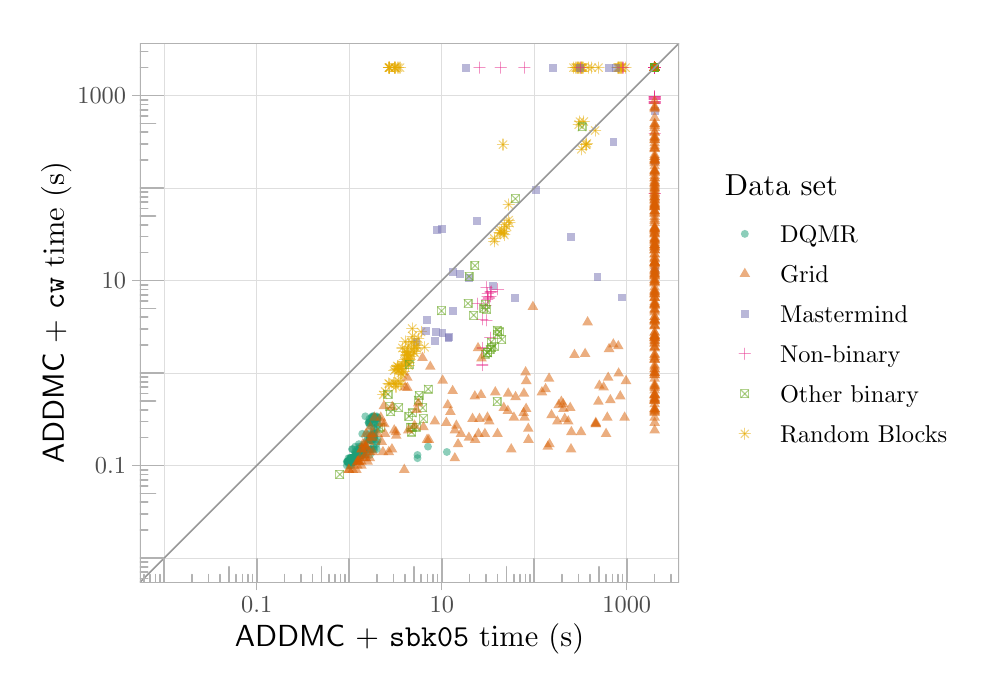
\begin{tikzpicture}[x=1pt,y=1pt]
\definecolor{fillColor}{RGB}{255,255,255}
\path[use as bounding box,fill=fillColor,fill opacity=0.00] (0,0) rectangle (343.28,231.26);
\begin{scope}
\path[clip] (  0.00,  0.09) rectangle (343.28,231.18);
\definecolor{drawColor}{RGB}{255,255,255}
\definecolor{fillColor}{RGB}{255,255,255}

\path[draw=drawColor,line width= 0.6pt,line join=round,line cap=round,fill=fillColor] (  0.00,  0.09) rectangle (343.28,231.18);
\end{scope}
\begin{scope}
\path[clip] ( 40.51, 30.77) rectangle (235.42,225.68);
\definecolor{fillColor}{RGB}{255,255,255}

\path[fill=fillColor] ( 40.51, 30.77) rectangle (235.42,225.68);
\definecolor{drawColor}{gray}{0.87}

\path[draw=drawColor,line width= 0.1pt,line join=round] ( 40.51, 39.63) --
	(235.42, 39.63);

\path[draw=drawColor,line width= 0.1pt,line join=round] ( 40.51,106.48) --
	(235.42,106.48);

\path[draw=drawColor,line width= 0.1pt,line join=round] ( 40.51,173.33) --
	(235.42,173.33);

\path[draw=drawColor,line width= 0.1pt,line join=round] ( 49.37, 30.77) --
	( 49.37,225.68);

\path[draw=drawColor,line width= 0.1pt,line join=round] (116.22, 30.77) --
	(116.22,225.68);

\path[draw=drawColor,line width= 0.1pt,line join=round] (183.07, 30.77) --
	(183.07,225.68);

\path[draw=drawColor,line width= 0.3pt,line join=round] ( 40.51, 73.06) --
	(235.42, 73.06);

\path[draw=drawColor,line width= 0.3pt,line join=round] ( 40.51,139.91) --
	(235.42,139.91);

\path[draw=drawColor,line width= 0.3pt,line join=round] ( 40.51,206.76) --
	(235.42,206.76);

\path[draw=drawColor,line width= 0.3pt,line join=round] ( 82.79, 30.77) --
	( 82.79,225.68);

\path[draw=drawColor,line width= 0.3pt,line join=round] (149.64, 30.77) --
	(149.64,225.68);

\path[draw=drawColor,line width= 0.3pt,line join=round] (216.49, 30.77) --
	(216.49,225.68);
\definecolor{drawColor}{RGB}{230,171,2}

\path[draw=drawColor,draw opacity=0.50,line width= 0.4pt,line join=round,line cap=round] (129.10,215.39) -- (131.96,218.25);

\path[draw=drawColor,draw opacity=0.50,line width= 0.4pt,line join=round,line cap=round] (129.10,218.25) -- (131.96,215.39);

\path[draw=drawColor,draw opacity=0.50,line width= 0.4pt,line join=round,line cap=round] (128.51,216.82) -- (132.55,216.82);

\path[draw=drawColor,draw opacity=0.50,line width= 0.4pt,line join=round,line cap=round] (130.53,214.80) -- (130.53,218.84);

\path[draw=drawColor,draw opacity=0.50,line width= 0.4pt,line join=round,line cap=round] (129.16,215.39) -- (132.01,218.25);

\path[draw=drawColor,draw opacity=0.50,line width= 0.4pt,line join=round,line cap=round] (129.16,218.25) -- (132.01,215.39);

\path[draw=drawColor,draw opacity=0.50,line width= 0.4pt,line join=round,line cap=round] (128.57,216.82) -- (132.60,216.82);

\path[draw=drawColor,draw opacity=0.50,line width= 0.4pt,line join=round,line cap=round] (130.58,214.80) -- (130.58,218.84);

\path[draw=drawColor,draw opacity=0.50,line width= 0.4pt,line join=round,line cap=round] (131.03,215.39) -- (133.88,218.25);

\path[draw=drawColor,draw opacity=0.50,line width= 0.4pt,line join=round,line cap=round] (131.03,218.25) -- (133.88,215.39);

\path[draw=drawColor,draw opacity=0.50,line width= 0.4pt,line join=round,line cap=round] (130.44,216.82) -- (134.47,216.82);

\path[draw=drawColor,draw opacity=0.50,line width= 0.4pt,line join=round,line cap=round] (132.45,214.80) -- (132.45,218.84);

\path[draw=drawColor,draw opacity=0.50,line width= 0.4pt,line join=round,line cap=round] (133.10,215.39) -- (135.96,218.25);

\path[draw=drawColor,draw opacity=0.50,line width= 0.4pt,line join=round,line cap=round] (133.10,218.25) -- (135.96,215.39);

\path[draw=drawColor,draw opacity=0.50,line width= 0.4pt,line join=round,line cap=round] (132.51,216.82) -- (136.55,216.82);

\path[draw=drawColor,draw opacity=0.50,line width= 0.4pt,line join=round,line cap=round] (134.53,214.80) -- (134.53,218.84);

\path[draw=drawColor,draw opacity=0.50,line width= 0.4pt,line join=round,line cap=round] (129.21,215.39) -- (132.06,218.25);

\path[draw=drawColor,draw opacity=0.50,line width= 0.4pt,line join=round,line cap=round] (129.21,218.25) -- (132.06,215.39);

\path[draw=drawColor,draw opacity=0.50,line width= 0.4pt,line join=round,line cap=round] (128.62,216.82) -- (132.66,216.82);

\path[draw=drawColor,draw opacity=0.50,line width= 0.4pt,line join=round,line cap=round] (130.64,214.80) -- (130.64,218.84);

\path[draw=drawColor,draw opacity=0.50,line width= 0.4pt,line join=round,line cap=round] (131.31,215.39) -- (134.16,218.25);

\path[draw=drawColor,draw opacity=0.50,line width= 0.4pt,line join=round,line cap=round] (131.31,218.25) -- (134.16,215.39);

\path[draw=drawColor,draw opacity=0.50,line width= 0.4pt,line join=round,line cap=round] (130.72,216.82) -- (134.75,216.82);

\path[draw=drawColor,draw opacity=0.50,line width= 0.4pt,line join=round,line cap=round] (132.74,214.80) -- (132.74,218.84);

\path[draw=drawColor,draw opacity=0.50,line width= 0.4pt,line join=round,line cap=round] (129.32,101.07) -- (132.17,103.92);

\path[draw=drawColor,draw opacity=0.50,line width= 0.4pt,line join=round,line cap=round] (129.32,103.92) -- (132.17,101.07);

\path[draw=drawColor,draw opacity=0.50,line width= 0.4pt,line join=round,line cap=round] (128.73,102.50) -- (132.76,102.50);

\path[draw=drawColor,draw opacity=0.50,line width= 0.4pt,line join=round,line cap=round] (130.75,100.48) -- (130.75,104.52);

\path[draw=drawColor,draw opacity=0.50,line width= 0.4pt,line join=round,line cap=round] (128.99,101.26) -- (131.85,104.11);

\path[draw=drawColor,draw opacity=0.50,line width= 0.4pt,line join=round,line cap=round] (128.99,104.11) -- (131.85,101.26);

\path[draw=drawColor,draw opacity=0.50,line width= 0.4pt,line join=round,line cap=round] (128.40,102.69) -- (132.44,102.69);

\path[draw=drawColor,draw opacity=0.50,line width= 0.4pt,line join=round,line cap=round] (130.42,100.67) -- (130.42,104.70);

\path[draw=drawColor,draw opacity=0.50,line width= 0.4pt,line join=round,line cap=round] (130.93,101.45) -- (133.79,104.30);

\path[draw=drawColor,draw opacity=0.50,line width= 0.4pt,line join=round,line cap=round] (130.93,104.30) -- (133.79,101.45);

\path[draw=drawColor,draw opacity=0.50,line width= 0.4pt,line join=round,line cap=round] (130.34,102.87) -- (134.38,102.87);

\path[draw=drawColor,draw opacity=0.50,line width= 0.4pt,line join=round,line cap=round] (132.36,100.86) -- (132.36,104.89);

\path[draw=drawColor,draw opacity=0.50,line width= 0.4pt,line join=round,line cap=round] (127.01, 97.15) -- (129.86,100.00);

\path[draw=drawColor,draw opacity=0.50,line width= 0.4pt,line join=round,line cap=round] (127.01,100.00) -- (129.86, 97.15);

\path[draw=drawColor,draw opacity=0.50,line width= 0.4pt,line join=round,line cap=round] (126.42, 98.57) -- (130.45, 98.57);

\path[draw=drawColor,draw opacity=0.50,line width= 0.4pt,line join=round,line cap=round] (128.44, 96.56) -- (128.44,100.59);

\path[draw=drawColor,draw opacity=0.50,line width= 0.4pt,line join=round,line cap=round] (127.80, 98.35) -- (130.65,101.20);

\path[draw=drawColor,draw opacity=0.50,line width= 0.4pt,line join=round,line cap=round] (127.80,101.20) -- (130.65, 98.35);

\path[draw=drawColor,draw opacity=0.50,line width= 0.4pt,line join=round,line cap=round] (127.21, 99.77) -- (131.25, 99.77);

\path[draw=drawColor,draw opacity=0.50,line width= 0.4pt,line join=round,line cap=round] (129.23, 97.76) -- (129.23,101.79);

\path[draw=drawColor,draw opacity=0.50,line width= 0.4pt,line join=round,line cap=round] (129.42,215.39) -- (132.28,218.25);

\path[draw=drawColor,draw opacity=0.50,line width= 0.4pt,line join=round,line cap=round] (129.42,218.25) -- (132.28,215.39);

\path[draw=drawColor,draw opacity=0.50,line width= 0.4pt,line join=round,line cap=round] (128.83,216.82) -- (132.87,216.82);

\path[draw=drawColor,draw opacity=0.50,line width= 0.4pt,line join=round,line cap=round] (130.85,214.80) -- (130.85,218.84);

\path[draw=drawColor,draw opacity=0.50,line width= 0.4pt,line join=round,line cap=round] (132.39,215.39) -- (135.24,218.25);

\path[draw=drawColor,draw opacity=0.50,line width= 0.4pt,line join=round,line cap=round] (132.39,218.25) -- (135.24,215.39);

\path[draw=drawColor,draw opacity=0.50,line width= 0.4pt,line join=round,line cap=round] (131.80,216.82) -- (135.83,216.82);

\path[draw=drawColor,draw opacity=0.50,line width= 0.4pt,line join=round,line cap=round] (133.81,214.80) -- (133.81,218.84);

\path[draw=drawColor,draw opacity=0.50,line width= 0.4pt,line join=round,line cap=round] (129.42,215.39) -- (132.28,218.25);

\path[draw=drawColor,draw opacity=0.50,line width= 0.4pt,line join=round,line cap=round] (129.42,218.25) -- (132.28,215.39);

\path[draw=drawColor,draw opacity=0.50,line width= 0.4pt,line join=round,line cap=round] (128.83,216.82) -- (132.87,216.82);

\path[draw=drawColor,draw opacity=0.50,line width= 0.4pt,line join=round,line cap=round] (130.85,214.80) -- (130.85,218.84);

\path[draw=drawColor,draw opacity=0.50,line width= 0.4pt,line join=round,line cap=round] (131.22,215.39) -- (134.07,218.25);

\path[draw=drawColor,draw opacity=0.50,line width= 0.4pt,line join=round,line cap=round] (131.22,218.25) -- (134.07,215.39);

\path[draw=drawColor,draw opacity=0.50,line width= 0.4pt,line join=round,line cap=round] (130.63,216.82) -- (134.66,216.82);

\path[draw=drawColor,draw opacity=0.50,line width= 0.4pt,line join=round,line cap=round] (132.64,214.80) -- (132.64,218.84);

\path[draw=drawColor,draw opacity=0.50,line width= 0.4pt,line join=round,line cap=round] (131.50,215.39) -- (134.35,218.25);

\path[draw=drawColor,draw opacity=0.50,line width= 0.4pt,line join=round,line cap=round] (131.50,218.25) -- (134.35,215.39);

\path[draw=drawColor,draw opacity=0.50,line width= 0.4pt,line join=round,line cap=round] (130.90,216.82) -- (134.94,216.82);

\path[draw=drawColor,draw opacity=0.50,line width= 0.4pt,line join=round,line cap=round] (132.92,214.80) -- (132.92,218.84);

\path[draw=drawColor,draw opacity=0.50,line width= 0.4pt,line join=round,line cap=round] (134.81,112.67) -- (137.66,115.53);

\path[draw=drawColor,draw opacity=0.50,line width= 0.4pt,line join=round,line cap=round] (134.81,115.53) -- (137.66,112.67);

\path[draw=drawColor,draw opacity=0.50,line width= 0.4pt,line join=round,line cap=round] (134.22,114.10) -- (138.25,114.10);

\path[draw=drawColor,draw opacity=0.50,line width= 0.4pt,line join=round,line cap=round] (136.23,112.08) -- (136.23,116.12);

\path[draw=drawColor,draw opacity=0.50,line width= 0.4pt,line join=round,line cap=round] (133.67,106.70) -- (136.52,109.55);

\path[draw=drawColor,draw opacity=0.50,line width= 0.4pt,line join=round,line cap=round] (133.67,109.55) -- (136.52,106.70);

\path[draw=drawColor,draw opacity=0.50,line width= 0.4pt,line join=round,line cap=round] (133.08,108.13) -- (137.11,108.13);

\path[draw=drawColor,draw opacity=0.50,line width= 0.4pt,line join=round,line cap=round] (135.09,106.11) -- (135.09,110.14);

\path[draw=drawColor,draw opacity=0.50,line width= 0.4pt,line join=round,line cap=round] (131.95,106.57) -- (134.80,109.42);

\path[draw=drawColor,draw opacity=0.50,line width= 0.4pt,line join=round,line cap=round] (131.95,109.42) -- (134.80,106.57);

\path[draw=drawColor,draw opacity=0.50,line width= 0.4pt,line join=round,line cap=round] (131.36,108.00) -- (135.39,108.00);

\path[draw=drawColor,draw opacity=0.50,line width= 0.4pt,line join=round,line cap=round] (133.37,105.98) -- (133.37,110.01);

\path[draw=drawColor,draw opacity=0.50,line width= 0.4pt,line join=round,line cap=round] (131.03,105.90) -- (133.88,108.75);

\path[draw=drawColor,draw opacity=0.50,line width= 0.4pt,line join=round,line cap=round] (131.03,108.75) -- (133.88,105.90);

\path[draw=drawColor,draw opacity=0.50,line width= 0.4pt,line join=round,line cap=round] (130.44,107.33) -- (134.47,107.33);

\path[draw=drawColor,draw opacity=0.50,line width= 0.4pt,line join=round,line cap=round] (132.45,105.31) -- (132.45,109.34);

\path[draw=drawColor,draw opacity=0.50,line width= 0.4pt,line join=round,line cap=round] (132.39,107.33) -- (135.24,110.19);

\path[draw=drawColor,draw opacity=0.50,line width= 0.4pt,line join=round,line cap=round] (132.39,110.19) -- (135.24,107.33);

\path[draw=drawColor,draw opacity=0.50,line width= 0.4pt,line join=round,line cap=round] (131.80,108.76) -- (135.83,108.76);

\path[draw=drawColor,draw opacity=0.50,line width= 0.4pt,line join=round,line cap=round] (133.81,106.74) -- (133.81,110.78);

\path[draw=drawColor,draw opacity=0.50,line width= 0.4pt,line join=round,line cap=round] (133.06,106.57) -- (135.91,109.42);

\path[draw=drawColor,draw opacity=0.50,line width= 0.4pt,line join=round,line cap=round] (133.06,109.42) -- (135.91,106.57);

\path[draw=drawColor,draw opacity=0.50,line width= 0.4pt,line join=round,line cap=round] (132.47,108.00) -- (136.51,108.00);

\path[draw=drawColor,draw opacity=0.50,line width= 0.4pt,line join=round,line cap=round] (134.49,105.98) -- (134.49,110.01);

\path[draw=drawColor,draw opacity=0.50,line width= 0.4pt,line join=round,line cap=round] (131.68,100.08) -- (134.53,102.94);

\path[draw=drawColor,draw opacity=0.50,line width= 0.4pt,line join=round,line cap=round] (131.68,102.94) -- (134.53,100.08);

\path[draw=drawColor,draw opacity=0.50,line width= 0.4pt,line join=round,line cap=round] (131.09,101.51) -- (135.12,101.51);

\path[draw=drawColor,draw opacity=0.50,line width= 0.4pt,line join=round,line cap=round] (133.10, 99.49) -- (133.10,103.53);

\path[draw=drawColor,draw opacity=0.50,line width= 0.4pt,line join=round,line cap=round] (133.47,101.07) -- (136.32,103.92);

\path[draw=drawColor,draw opacity=0.50,line width= 0.4pt,line join=round,line cap=round] (133.47,103.92) -- (136.32,101.07);

\path[draw=drawColor,draw opacity=0.50,line width= 0.4pt,line join=round,line cap=round] (132.88,102.50) -- (136.91,102.50);

\path[draw=drawColor,draw opacity=0.50,line width= 0.4pt,line join=round,line cap=round] (134.89,100.48) -- (134.89,104.52);

\path[draw=drawColor,draw opacity=0.50,line width= 0.4pt,line join=round,line cap=round] (131.36,101.07) -- (134.21,103.92);

\path[draw=drawColor,draw opacity=0.50,line width= 0.4pt,line join=round,line cap=round] (131.36,103.92) -- (134.21,101.07);

\path[draw=drawColor,draw opacity=0.50,line width= 0.4pt,line join=round,line cap=round] (130.77,102.50) -- (134.80,102.50);

\path[draw=drawColor,draw opacity=0.50,line width= 0.4pt,line join=round,line cap=round] (132.78,100.48) -- (132.78,104.52);

\path[draw=drawColor,draw opacity=0.50,line width= 0.4pt,line join=round,line cap=round] (134.06,104.46) -- (136.91,107.32);

\path[draw=drawColor,draw opacity=0.50,line width= 0.4pt,line join=round,line cap=round] (134.06,107.32) -- (136.91,104.46);

\path[draw=drawColor,draw opacity=0.50,line width= 0.4pt,line join=round,line cap=round] (133.47,105.89) -- (137.50,105.89);

\path[draw=drawColor,draw opacity=0.50,line width= 0.4pt,line join=round,line cap=round] (135.48,103.87) -- (135.48,107.91);

\path[draw=drawColor,draw opacity=0.50,line width= 0.4pt,line join=round,line cap=round] (132.56,102.17) -- (135.41,105.03);

\path[draw=drawColor,draw opacity=0.50,line width= 0.4pt,line join=round,line cap=round] (132.56,105.03) -- (135.41,102.17);

\path[draw=drawColor,draw opacity=0.50,line width= 0.4pt,line join=round,line cap=round] (131.97,103.60) -- (136.00,103.60);

\path[draw=drawColor,draw opacity=0.50,line width= 0.4pt,line join=round,line cap=round] (133.98,101.58) -- (133.98,105.62);

\path[draw=drawColor,draw opacity=0.50,line width= 0.4pt,line join=round,line cap=round] (132.52,106.17) -- (135.37,109.03);

\path[draw=drawColor,draw opacity=0.50,line width= 0.4pt,line join=round,line cap=round] (132.52,109.03) -- (135.37,106.17);

\path[draw=drawColor,draw opacity=0.50,line width= 0.4pt,line join=round,line cap=round] (131.92,107.60) -- (135.96,107.60);

\path[draw=drawColor,draw opacity=0.50,line width= 0.4pt,line join=round,line cap=round] (133.94,105.58) -- (133.94,109.62);

\path[draw=drawColor,draw opacity=0.50,line width= 0.4pt,line join=round,line cap=round] (131.45,106.44) -- (134.30,109.29);

\path[draw=drawColor,draw opacity=0.50,line width= 0.4pt,line join=round,line cap=round] (131.45,109.29) -- (134.30,106.44);

\path[draw=drawColor,draw opacity=0.50,line width= 0.4pt,line join=round,line cap=round] (130.86,107.86) -- (134.89,107.86);

\path[draw=drawColor,draw opacity=0.50,line width= 0.4pt,line join=round,line cap=round] (132.88,105.85) -- (132.88,109.88);

\path[draw=drawColor,draw opacity=0.50,line width= 0.4pt,line join=round,line cap=round] (134.02,107.94) -- (136.87,110.79);

\path[draw=drawColor,draw opacity=0.50,line width= 0.4pt,line join=round,line cap=round] (134.02,110.79) -- (136.87,107.94);

\path[draw=drawColor,draw opacity=0.50,line width= 0.4pt,line join=round,line cap=round] (133.43,109.37) -- (137.46,109.37);

\path[draw=drawColor,draw opacity=0.50,line width= 0.4pt,line join=round,line cap=round] (135.45,107.35) -- (135.45,111.39);

\path[draw=drawColor,draw opacity=0.50,line width= 0.4pt,line join=round,line cap=round] (132.08,107.58) -- (134.93,110.43);

\path[draw=drawColor,draw opacity=0.50,line width= 0.4pt,line join=round,line cap=round] (132.08,110.43) -- (134.93,107.58);

\path[draw=drawColor,draw opacity=0.50,line width= 0.4pt,line join=round,line cap=round] (131.49,109.01) -- (135.52,109.01);

\path[draw=drawColor,draw opacity=0.50,line width= 0.4pt,line join=round,line cap=round] (133.51,106.99) -- (133.51,111.02);

\path[draw=drawColor,draw opacity=0.50,line width= 0.4pt,line join=round,line cap=round] (133.63,107.33) -- (136.48,110.19);

\path[draw=drawColor,draw opacity=0.50,line width= 0.4pt,line join=round,line cap=round] (133.63,110.19) -- (136.48,107.33);

\path[draw=drawColor,draw opacity=0.50,line width= 0.4pt,line join=round,line cap=round] (133.04,108.76) -- (137.07,108.76);

\path[draw=drawColor,draw opacity=0.50,line width= 0.4pt,line join=round,line cap=round] (135.05,106.74) -- (135.05,110.78);

\path[draw=drawColor,draw opacity=0.50,line width= 0.4pt,line join=round,line cap=round] (138.47,112.24) -- (141.33,115.09);

\path[draw=drawColor,draw opacity=0.50,line width= 0.4pt,line join=round,line cap=round] (138.47,115.09) -- (141.33,112.24);

\path[draw=drawColor,draw opacity=0.50,line width= 0.4pt,line join=round,line cap=round] (137.88,113.66) -- (141.92,113.66);

\path[draw=drawColor,draw opacity=0.50,line width= 0.4pt,line join=round,line cap=round] (139.90,111.64) -- (139.90,115.68);

\path[draw=drawColor,draw opacity=0.50,line width= 0.4pt,line join=round,line cap=round] (136.91,111.04) -- (139.77,113.89);

\path[draw=drawColor,draw opacity=0.50,line width= 0.4pt,line join=round,line cap=round] (136.91,113.89) -- (139.77,111.04);

\path[draw=drawColor,draw opacity=0.50,line width= 0.4pt,line join=round,line cap=round] (136.32,112.46) -- (140.36,112.46);

\path[draw=drawColor,draw opacity=0.50,line width= 0.4pt,line join=round,line cap=round] (138.34,110.45) -- (138.34,114.48);

\path[draw=drawColor,draw opacity=0.50,line width= 0.4pt,line join=round,line cap=round] (136.10,114.75) -- (138.95,117.60);

\path[draw=drawColor,draw opacity=0.50,line width= 0.4pt,line join=round,line cap=round] (136.10,117.60) -- (138.95,114.75);

\path[draw=drawColor,draw opacity=0.50,line width= 0.4pt,line join=round,line cap=round] (135.51,116.18) -- (139.55,116.18);

\path[draw=drawColor,draw opacity=0.50,line width= 0.4pt,line join=round,line cap=round] (137.53,114.16) -- (137.53,118.19);

\path[draw=drawColor,draw opacity=0.50,line width= 0.4pt,line join=round,line cap=round] (138.13,112.67) -- (140.98,115.53);

\path[draw=drawColor,draw opacity=0.50,line width= 0.4pt,line join=round,line cap=round] (138.13,115.53) -- (140.98,112.67);

\path[draw=drawColor,draw opacity=0.50,line width= 0.4pt,line join=round,line cap=round] (137.54,114.10) -- (141.57,114.10);

\path[draw=drawColor,draw opacity=0.50,line width= 0.4pt,line join=round,line cap=round] (139.55,112.08) -- (139.55,116.12);

\path[draw=drawColor,draw opacity=0.50,line width= 0.4pt,line join=round,line cap=round] (138.39,116.50) -- (141.24,119.35);

\path[draw=drawColor,draw opacity=0.50,line width= 0.4pt,line join=round,line cap=round] (138.39,119.35) -- (141.24,116.50);

\path[draw=drawColor,draw opacity=0.50,line width= 0.4pt,line join=round,line cap=round] (137.80,117.93) -- (141.83,117.93);

\path[draw=drawColor,draw opacity=0.50,line width= 0.4pt,line join=round,line cap=round] (139.81,115.91) -- (139.81,119.94);

\path[draw=drawColor,draw opacity=0.50,line width= 0.4pt,line join=round,line cap=round] (135.83,111.42) -- (138.68,114.27);

\path[draw=drawColor,draw opacity=0.50,line width= 0.4pt,line join=round,line cap=round] (135.83,114.27) -- (138.68,111.42);

\path[draw=drawColor,draw opacity=0.50,line width= 0.4pt,line join=round,line cap=round] (135.24,112.84) -- (139.28,112.84);

\path[draw=drawColor,draw opacity=0.50,line width= 0.4pt,line join=round,line cap=round] (137.26,110.83) -- (137.26,114.86);

\path[draw=drawColor,draw opacity=0.50,line width= 0.4pt,line join=round,line cap=round] (135.42,111.60) -- (138.27,114.46);

\path[draw=drawColor,draw opacity=0.50,line width= 0.4pt,line join=round,line cap=round] (135.42,114.46) -- (138.27,111.60);

\path[draw=drawColor,draw opacity=0.50,line width= 0.4pt,line join=round,line cap=round] (134.83,113.03) -- (138.86,113.03);

\path[draw=drawColor,draw opacity=0.50,line width= 0.4pt,line join=round,line cap=round] (136.84,111.01) -- (136.84,115.05);

\path[draw=drawColor,draw opacity=0.50,line width= 0.4pt,line join=round,line cap=round] (133.47,105.05) -- (136.32,107.91);

\path[draw=drawColor,draw opacity=0.50,line width= 0.4pt,line join=round,line cap=round] (133.47,107.91) -- (136.32,105.05);

\path[draw=drawColor,draw opacity=0.50,line width= 0.4pt,line join=round,line cap=round] (132.88,106.48) -- (136.91,106.48);

\path[draw=drawColor,draw opacity=0.50,line width= 0.4pt,line join=round,line cap=round] (134.89,104.46) -- (134.89,108.50);

\path[draw=drawColor,draw opacity=0.50,line width= 0.4pt,line join=round,line cap=round] (136.27,107.70) -- (139.12,110.55);

\path[draw=drawColor,draw opacity=0.50,line width= 0.4pt,line join=round,line cap=round] (136.27,110.55) -- (139.12,107.70);

\path[draw=drawColor,draw opacity=0.50,line width= 0.4pt,line join=round,line cap=round] (135.68,109.13) -- (139.71,109.13);

\path[draw=drawColor,draw opacity=0.50,line width= 0.4pt,line join=round,line cap=round] (137.69,107.11) -- (137.69,111.15);

\path[draw=drawColor,draw opacity=0.50,line width= 0.4pt,line join=round,line cap=round] (135.73,112.59) -- (138.58,115.44);

\path[draw=drawColor,draw opacity=0.50,line width= 0.4pt,line join=round,line cap=round] (135.73,115.44) -- (138.58,112.59);

\path[draw=drawColor,draw opacity=0.50,line width= 0.4pt,line join=round,line cap=round] (135.14,114.01) -- (139.17,114.01);

\path[draw=drawColor,draw opacity=0.50,line width= 0.4pt,line join=round,line cap=round] (137.16,111.99) -- (137.16,116.03);

\path[draw=drawColor,draw opacity=0.50,line width= 0.4pt,line join=round,line cap=round] (134.47,105.48) -- (137.33,108.34);

\path[draw=drawColor,draw opacity=0.50,line width= 0.4pt,line join=round,line cap=round] (134.47,108.34) -- (137.33,105.48);

\path[draw=drawColor,draw opacity=0.50,line width= 0.4pt,line join=round,line cap=round] (133.88,106.91) -- (137.92,106.91);

\path[draw=drawColor,draw opacity=0.50,line width= 0.4pt,line join=round,line cap=round] (135.90,104.89) -- (135.90,108.93);

\path[draw=drawColor,draw opacity=0.50,line width= 0.4pt,line join=round,line cap=round] (137.53,121.10) -- (140.39,123.95);

\path[draw=drawColor,draw opacity=0.50,line width= 0.4pt,line join=round,line cap=round] (137.53,123.95) -- (140.39,121.10);

\path[draw=drawColor,draw opacity=0.50,line width= 0.4pt,line join=round,line cap=round] (136.94,122.53) -- (140.98,122.53);

\path[draw=drawColor,draw opacity=0.50,line width= 0.4pt,line join=round,line cap=round] (138.96,120.51) -- (138.96,124.54);

\path[draw=drawColor,draw opacity=0.50,line width= 0.4pt,line join=round,line cap=round] (134.95,116.43) -- (137.81,119.29);

\path[draw=drawColor,draw opacity=0.50,line width= 0.4pt,line join=round,line cap=round] (134.95,119.29) -- (137.81,116.43);

\path[draw=drawColor,draw opacity=0.50,line width= 0.4pt,line join=round,line cap=round] (134.36,117.86) -- (138.40,117.86);

\path[draw=drawColor,draw opacity=0.50,line width= 0.4pt,line join=round,line cap=round] (136.38,115.84) -- (136.38,119.88);

\path[draw=drawColor,draw opacity=0.50,line width= 0.4pt,line join=round,line cap=round] (134.84,109.84) -- (137.70,112.69);

\path[draw=drawColor,draw opacity=0.50,line width= 0.4pt,line join=round,line cap=round] (134.84,112.69) -- (137.70,109.84);

\path[draw=drawColor,draw opacity=0.50,line width= 0.4pt,line join=round,line cap=round] (134.25,111.26) -- (138.29,111.26);

\path[draw=drawColor,draw opacity=0.50,line width= 0.4pt,line join=round,line cap=round] (136.27,109.24) -- (136.27,113.28);

\path[draw=drawColor,draw opacity=0.50,line width= 0.4pt,line join=round,line cap=round] (134.73,109.19) -- (137.59,112.05);

\path[draw=drawColor,draw opacity=0.50,line width= 0.4pt,line join=round,line cap=round] (134.73,112.05) -- (137.59,109.19);

\path[draw=drawColor,draw opacity=0.50,line width= 0.4pt,line join=round,line cap=round] (134.14,110.62) -- (138.18,110.62);

\path[draw=drawColor,draw opacity=0.50,line width= 0.4pt,line join=round,line cap=round] (136.16,108.60) -- (136.16,112.64);

\path[draw=drawColor,draw opacity=0.50,line width= 0.4pt,line join=round,line cap=round] (135.97,111.23) -- (138.82,114.08);

\path[draw=drawColor,draw opacity=0.50,line width= 0.4pt,line join=round,line cap=round] (135.97,114.08) -- (138.82,111.23);

\path[draw=drawColor,draw opacity=0.50,line width= 0.4pt,line join=round,line cap=round] (135.38,112.65) -- (139.41,112.65);

\path[draw=drawColor,draw opacity=0.50,line width= 0.4pt,line join=round,line cap=round] (137.39,110.64) -- (137.39,114.67);

\path[draw=drawColor,draw opacity=0.50,line width= 0.4pt,line join=round,line cap=round] (225.13,215.39) -- (227.98,218.25);

\path[draw=drawColor,draw opacity=0.50,line width= 0.4pt,line join=round,line cap=round] (225.13,218.25) -- (227.98,215.39);

\path[draw=drawColor,draw opacity=0.50,line width= 0.4pt,line join=round,line cap=round] (224.54,216.82) -- (228.57,216.82);

\path[draw=drawColor,draw opacity=0.50,line width= 0.4pt,line join=round,line cap=round] (226.56,214.80) -- (226.56,218.84);

\path[draw=drawColor,draw opacity=0.50,line width= 0.4pt,line join=round,line cap=round] (225.13,215.39) -- (227.98,218.25);

\path[draw=drawColor,draw opacity=0.50,line width= 0.4pt,line join=round,line cap=round] (225.13,218.25) -- (227.98,215.39);

\path[draw=drawColor,draw opacity=0.50,line width= 0.4pt,line join=round,line cap=round] (224.54,216.82) -- (228.57,216.82);

\path[draw=drawColor,draw opacity=0.50,line width= 0.4pt,line join=round,line cap=round] (226.56,214.80) -- (226.56,218.84);

\path[draw=drawColor,draw opacity=0.50,line width= 0.4pt,line join=round,line cap=round] (225.13,215.39) -- (227.98,218.25);

\path[draw=drawColor,draw opacity=0.50,line width= 0.4pt,line join=round,line cap=round] (225.13,218.25) -- (227.98,215.39);

\path[draw=drawColor,draw opacity=0.50,line width= 0.4pt,line join=round,line cap=round] (224.54,216.82) -- (228.57,216.82);

\path[draw=drawColor,draw opacity=0.50,line width= 0.4pt,line join=round,line cap=round] (226.56,214.80) -- (226.56,218.84);

\path[draw=drawColor,draw opacity=0.50,line width= 0.4pt,line join=round,line cap=round] (225.13,215.39) -- (227.98,218.25);

\path[draw=drawColor,draw opacity=0.50,line width= 0.4pt,line join=round,line cap=round] (225.13,218.25) -- (227.98,215.39);

\path[draw=drawColor,draw opacity=0.50,line width= 0.4pt,line join=round,line cap=round] (224.54,216.82) -- (228.57,216.82);

\path[draw=drawColor,draw opacity=0.50,line width= 0.4pt,line join=round,line cap=round] (226.56,214.80) -- (226.56,218.84);

\path[draw=drawColor,draw opacity=0.50,line width= 0.4pt,line join=round,line cap=round] (225.13,215.39) -- (227.98,218.25);

\path[draw=drawColor,draw opacity=0.50,line width= 0.4pt,line join=round,line cap=round] (225.13,218.25) -- (227.98,215.39);

\path[draw=drawColor,draw opacity=0.50,line width= 0.4pt,line join=round,line cap=round] (224.54,216.82) -- (228.57,216.82);

\path[draw=drawColor,draw opacity=0.50,line width= 0.4pt,line join=round,line cap=round] (226.56,214.80) -- (226.56,218.84);

\path[draw=drawColor,draw opacity=0.50,line width= 0.4pt,line join=round,line cap=round] (225.13,215.39) -- (227.98,218.25);

\path[draw=drawColor,draw opacity=0.50,line width= 0.4pt,line join=round,line cap=round] (225.13,218.25) -- (227.98,215.39);

\path[draw=drawColor,draw opacity=0.50,line width= 0.4pt,line join=round,line cap=round] (224.54,216.82) -- (228.57,216.82);

\path[draw=drawColor,draw opacity=0.50,line width= 0.4pt,line join=round,line cap=round] (226.56,214.80) -- (226.56,218.84);

\path[draw=drawColor,draw opacity=0.50,line width= 0.4pt,line join=round,line cap=round] (170.33,187.58) -- (173.18,190.43);

\path[draw=drawColor,draw opacity=0.50,line width= 0.4pt,line join=round,line cap=round] (170.33,190.43) -- (173.18,187.58);

\path[draw=drawColor,draw opacity=0.50,line width= 0.4pt,line join=round,line cap=round] (169.74,189.01) -- (173.77,189.01);

\path[draw=drawColor,draw opacity=0.50,line width= 0.4pt,line join=round,line cap=round] (171.76,186.99) -- (171.76,191.02);

\path[draw=drawColor,draw opacity=0.50,line width= 0.4pt,line join=round,line cap=round] (169.07,155.90) -- (171.93,158.76);

\path[draw=drawColor,draw opacity=0.50,line width= 0.4pt,line join=round,line cap=round] (169.07,158.76) -- (171.93,155.90);

\path[draw=drawColor,draw opacity=0.50,line width= 0.4pt,line join=round,line cap=round] (168.48,157.33) -- (172.52,157.33);

\path[draw=drawColor,draw opacity=0.50,line width= 0.4pt,line join=round,line cap=round] (170.50,155.31) -- (170.50,159.35);

\path[draw=drawColor,draw opacity=0.50,line width= 0.4pt,line join=round,line cap=round] (167.16,152.68) -- (170.01,155.53);

\path[draw=drawColor,draw opacity=0.50,line width= 0.4pt,line join=round,line cap=round] (167.16,155.53) -- (170.01,152.68);

\path[draw=drawColor,draw opacity=0.50,line width= 0.4pt,line join=round,line cap=round] (166.57,154.11) -- (170.60,154.11);

\path[draw=drawColor,draw opacity=0.50,line width= 0.4pt,line join=round,line cap=round] (168.59,152.09) -- (168.59,156.13);

\path[draw=drawColor,draw opacity=0.50,line width= 0.4pt,line join=round,line cap=round] (170.77,156.31) -- (173.62,159.16);

\path[draw=drawColor,draw opacity=0.50,line width= 0.4pt,line join=round,line cap=round] (170.77,159.16) -- (173.62,156.31);

\path[draw=drawColor,draw opacity=0.50,line width= 0.4pt,line join=round,line cap=round] (170.18,157.74) -- (174.21,157.74);

\path[draw=drawColor,draw opacity=0.50,line width= 0.4pt,line join=round,line cap=round] (172.19,155.72) -- (172.19,159.75);

\path[draw=drawColor,draw opacity=0.50,line width= 0.4pt,line join=round,line cap=round] (167.12,153.70) -- (169.98,156.55);

\path[draw=drawColor,draw opacity=0.50,line width= 0.4pt,line join=round,line cap=round] (167.12,156.55) -- (169.98,153.70);

\path[draw=drawColor,draw opacity=0.50,line width= 0.4pt,line join=round,line cap=round] (166.53,155.12) -- (170.57,155.12);

\path[draw=drawColor,draw opacity=0.50,line width= 0.4pt,line join=round,line cap=round] (168.55,153.11) -- (168.55,157.14);

\path[draw=drawColor,draw opacity=0.50,line width= 0.4pt,line join=round,line cap=round] (225.13,215.39) -- (227.98,218.25);

\path[draw=drawColor,draw opacity=0.50,line width= 0.4pt,line join=round,line cap=round] (225.13,218.25) -- (227.98,215.39);

\path[draw=drawColor,draw opacity=0.50,line width= 0.4pt,line join=round,line cap=round] (224.54,216.82) -- (228.57,216.82);

\path[draw=drawColor,draw opacity=0.50,line width= 0.4pt,line join=round,line cap=round] (226.56,214.80) -- (226.56,218.84);

\path[draw=drawColor,draw opacity=0.50,line width= 0.4pt,line join=round,line cap=round] (225.13,215.39) -- (227.98,218.25);

\path[draw=drawColor,draw opacity=0.50,line width= 0.4pt,line join=round,line cap=round] (225.13,218.25) -- (227.98,215.39);

\path[draw=drawColor,draw opacity=0.50,line width= 0.4pt,line join=round,line cap=round] (224.54,216.82) -- (228.57,216.82);

\path[draw=drawColor,draw opacity=0.50,line width= 0.4pt,line join=round,line cap=round] (226.56,214.80) -- (226.56,218.84);

\path[draw=drawColor,draw opacity=0.50,line width= 0.4pt,line join=round,line cap=round] (225.13,215.39) -- (227.98,218.25);

\path[draw=drawColor,draw opacity=0.50,line width= 0.4pt,line join=round,line cap=round] (225.13,218.25) -- (227.98,215.39);

\path[draw=drawColor,draw opacity=0.50,line width= 0.4pt,line join=round,line cap=round] (224.54,216.82) -- (228.57,216.82);

\path[draw=drawColor,draw opacity=0.50,line width= 0.4pt,line join=round,line cap=round] (226.56,214.80) -- (226.56,218.84);

\path[draw=drawColor,draw opacity=0.50,line width= 0.4pt,line join=round,line cap=round] (225.13,215.39) -- (227.98,218.25);

\path[draw=drawColor,draw opacity=0.50,line width= 0.4pt,line join=round,line cap=round] (225.13,218.25) -- (227.98,215.39);

\path[draw=drawColor,draw opacity=0.50,line width= 0.4pt,line join=round,line cap=round] (224.54,216.82) -- (228.57,216.82);

\path[draw=drawColor,draw opacity=0.50,line width= 0.4pt,line join=round,line cap=round] (226.56,214.80) -- (226.56,218.84);

\path[draw=drawColor,draw opacity=0.50,line width= 0.4pt,line join=round,line cap=round] (225.13,215.39) -- (227.98,218.25);

\path[draw=drawColor,draw opacity=0.50,line width= 0.4pt,line join=round,line cap=round] (225.13,218.25) -- (227.98,215.39);

\path[draw=drawColor,draw opacity=0.50,line width= 0.4pt,line join=round,line cap=round] (224.54,216.82) -- (228.57,216.82);

\path[draw=drawColor,draw opacity=0.50,line width= 0.4pt,line join=round,line cap=round] (226.56,214.80) -- (226.56,218.84);

\path[draw=drawColor,draw opacity=0.50,line width= 0.4pt,line join=round,line cap=round] (198.59,215.39) -- (201.44,218.25);

\path[draw=drawColor,draw opacity=0.50,line width= 0.4pt,line join=round,line cap=round] (198.59,218.25) -- (201.44,215.39);

\path[draw=drawColor,draw opacity=0.50,line width= 0.4pt,line join=round,line cap=round] (198.00,216.82) -- (202.04,216.82);

\path[draw=drawColor,draw opacity=0.50,line width= 0.4pt,line join=round,line cap=round] (200.02,214.80) -- (200.02,218.84);

\path[draw=drawColor,draw opacity=0.50,line width= 0.4pt,line join=round,line cap=round] (198.49,215.39) -- (201.34,218.25);

\path[draw=drawColor,draw opacity=0.50,line width= 0.4pt,line join=round,line cap=round] (198.49,218.25) -- (201.34,215.39);

\path[draw=drawColor,draw opacity=0.50,line width= 0.4pt,line join=round,line cap=round] (197.90,216.82) -- (201.93,216.82);

\path[draw=drawColor,draw opacity=0.50,line width= 0.4pt,line join=round,line cap=round] (199.91,214.80) -- (199.91,218.84);

\path[draw=drawColor,draw opacity=0.50,line width= 0.4pt,line join=round,line cap=round] (201.11,215.39) -- (203.97,218.25);

\path[draw=drawColor,draw opacity=0.50,line width= 0.4pt,line join=round,line cap=round] (201.11,218.25) -- (203.97,215.39);

\path[draw=drawColor,draw opacity=0.50,line width= 0.4pt,line join=round,line cap=round] (200.52,216.82) -- (204.56,216.82);

\path[draw=drawColor,draw opacity=0.50,line width= 0.4pt,line join=round,line cap=round] (202.54,214.80) -- (202.54,218.84);

\path[draw=drawColor,draw opacity=0.50,line width= 0.4pt,line join=round,line cap=round] (198.62,215.39) -- (201.47,218.25);

\path[draw=drawColor,draw opacity=0.50,line width= 0.4pt,line join=round,line cap=round] (198.62,218.25) -- (201.47,215.39);

\path[draw=drawColor,draw opacity=0.50,line width= 0.4pt,line join=round,line cap=round] (198.03,216.82) -- (202.06,216.82);

\path[draw=drawColor,draw opacity=0.50,line width= 0.4pt,line join=round,line cap=round] (200.04,214.80) -- (200.04,218.84);

\path[draw=drawColor,draw opacity=0.50,line width= 0.4pt,line join=round,line cap=round] (199.02,215.39) -- (201.88,218.25);

\path[draw=drawColor,draw opacity=0.50,line width= 0.4pt,line join=round,line cap=round] (199.02,218.25) -- (201.88,215.39);

\path[draw=drawColor,draw opacity=0.50,line width= 0.4pt,line join=round,line cap=round] (198.43,216.82) -- (202.47,216.82);

\path[draw=drawColor,draw opacity=0.50,line width= 0.4pt,line join=round,line cap=round] (200.45,214.80) -- (200.45,218.84);

\path[draw=drawColor,draw opacity=0.50,line width= 0.4pt,line join=round,line cap=round] (197.58,215.39) -- (200.43,218.25);

\path[draw=drawColor,draw opacity=0.50,line width= 0.4pt,line join=round,line cap=round] (197.58,218.25) -- (200.43,215.39);

\path[draw=drawColor,draw opacity=0.50,line width= 0.4pt,line join=round,line cap=round] (196.98,216.82) -- (201.02,216.82);

\path[draw=drawColor,draw opacity=0.50,line width= 0.4pt,line join=round,line cap=round] (199.00,214.80) -- (199.00,218.84);

\path[draw=drawColor,draw opacity=0.50,line width= 0.4pt,line join=round,line cap=round] (170.36,155.61) -- (173.22,158.47);

\path[draw=drawColor,draw opacity=0.50,line width= 0.4pt,line join=round,line cap=round] (170.36,158.47) -- (173.22,155.61);

\path[draw=drawColor,draw opacity=0.50,line width= 0.4pt,line join=round,line cap=round] (169.77,157.04) -- (173.81,157.04);

\path[draw=drawColor,draw opacity=0.50,line width= 0.4pt,line join=round,line cap=round] (171.79,155.02) -- (171.79,159.06);

\path[draw=drawColor,draw opacity=0.50,line width= 0.4pt,line join=round,line cap=round] (170.84,158.55) -- (173.70,161.41);

\path[draw=drawColor,draw opacity=0.50,line width= 0.4pt,line join=round,line cap=round] (170.84,161.41) -- (173.70,158.55);

\path[draw=drawColor,draw opacity=0.50,line width= 0.4pt,line join=round,line cap=round] (170.25,159.98) -- (174.29,159.98);

\path[draw=drawColor,draw opacity=0.50,line width= 0.4pt,line join=round,line cap=round] (172.27,157.96) -- (172.27,162.00);

\path[draw=drawColor,draw opacity=0.50,line width= 0.4pt,line join=round,line cap=round] (170.78,154.94) -- (173.63,157.79);

\path[draw=drawColor,draw opacity=0.50,line width= 0.4pt,line join=round,line cap=round] (170.78,157.79) -- (173.63,154.94);

\path[draw=drawColor,draw opacity=0.50,line width= 0.4pt,line join=round,line cap=round] (170.18,156.37) -- (174.22,156.37);

\path[draw=drawColor,draw opacity=0.50,line width= 0.4pt,line join=round,line cap=round] (172.20,154.35) -- (172.20,158.39);

\path[draw=drawColor,draw opacity=0.50,line width= 0.4pt,line join=round,line cap=round] (169.67,156.62) -- (172.52,159.47);

\path[draw=drawColor,draw opacity=0.50,line width= 0.4pt,line join=round,line cap=round] (169.67,159.47) -- (172.52,156.62);

\path[draw=drawColor,draw opacity=0.50,line width= 0.4pt,line join=round,line cap=round] (169.08,158.04) -- (173.11,158.04);

\path[draw=drawColor,draw opacity=0.50,line width= 0.4pt,line join=round,line cap=round] (171.10,156.02) -- (171.10,160.06);

\path[draw=drawColor,draw opacity=0.50,line width= 0.4pt,line join=round,line cap=round] (169.54,155.64) -- (172.39,158.49);

\path[draw=drawColor,draw opacity=0.50,line width= 0.4pt,line join=round,line cap=round] (169.54,158.49) -- (172.39,155.64);

\path[draw=drawColor,draw opacity=0.50,line width= 0.4pt,line join=round,line cap=round] (168.95,157.07) -- (172.98,157.07);

\path[draw=drawColor,draw opacity=0.50,line width= 0.4pt,line join=round,line cap=round] (170.97,155.05) -- (170.97,159.08);

\path[draw=drawColor,draw opacity=0.50,line width= 0.4pt,line join=round,line cap=round] (196.80,215.39) -- (199.65,218.25);

\path[draw=drawColor,draw opacity=0.50,line width= 0.4pt,line join=round,line cap=round] (196.80,218.25) -- (199.65,215.39);

\path[draw=drawColor,draw opacity=0.50,line width= 0.4pt,line join=round,line cap=round] (196.21,216.82) -- (200.24,216.82);

\path[draw=drawColor,draw opacity=0.50,line width= 0.4pt,line join=round,line cap=round] (198.23,214.80) -- (198.23,218.84);

\path[draw=drawColor,draw opacity=0.50,line width= 0.4pt,line join=round,line cap=round] (196.61,215.39) -- (199.47,218.25);

\path[draw=drawColor,draw opacity=0.50,line width= 0.4pt,line join=round,line cap=round] (196.61,218.25) -- (199.47,215.39);

\path[draw=drawColor,draw opacity=0.50,line width= 0.4pt,line join=round,line cap=round] (196.02,216.82) -- (200.06,216.82);

\path[draw=drawColor,draw opacity=0.50,line width= 0.4pt,line join=round,line cap=round] (198.04,214.80) -- (198.04,218.84);

\path[draw=drawColor,draw opacity=0.50,line width= 0.4pt,line join=round,line cap=round] (198.67,215.39) -- (201.53,218.25);

\path[draw=drawColor,draw opacity=0.50,line width= 0.4pt,line join=round,line cap=round] (198.67,218.25) -- (201.53,215.39);

\path[draw=drawColor,draw opacity=0.50,line width= 0.4pt,line join=round,line cap=round] (198.08,216.82) -- (202.12,216.82);

\path[draw=drawColor,draw opacity=0.50,line width= 0.4pt,line join=round,line cap=round] (200.10,214.80) -- (200.10,218.84);

\path[draw=drawColor,draw opacity=0.50,line width= 0.4pt,line join=round,line cap=round] (197.33,215.39) -- (200.19,218.25);

\path[draw=drawColor,draw opacity=0.50,line width= 0.4pt,line join=round,line cap=round] (197.33,218.25) -- (200.19,215.39);

\path[draw=drawColor,draw opacity=0.50,line width= 0.4pt,line join=round,line cap=round] (196.74,216.82) -- (200.78,216.82);

\path[draw=drawColor,draw opacity=0.50,line width= 0.4pt,line join=round,line cap=round] (198.76,214.80) -- (198.76,218.84);

\path[draw=drawColor,draw opacity=0.50,line width= 0.4pt,line join=round,line cap=round] (197.23,215.39) -- (200.08,218.25);

\path[draw=drawColor,draw opacity=0.50,line width= 0.4pt,line join=round,line cap=round] (197.23,218.25) -- (200.08,215.39);

\path[draw=drawColor,draw opacity=0.50,line width= 0.4pt,line join=round,line cap=round] (196.64,216.82) -- (200.67,216.82);

\path[draw=drawColor,draw opacity=0.50,line width= 0.4pt,line join=round,line cap=round] (198.65,214.80) -- (198.65,218.84);

\path[draw=drawColor,draw opacity=0.50,line width= 0.4pt,line join=round,line cap=round] (225.13,215.39) -- (227.98,218.25);

\path[draw=drawColor,draw opacity=0.50,line width= 0.4pt,line join=round,line cap=round] (225.13,218.25) -- (227.98,215.39);

\path[draw=drawColor,draw opacity=0.50,line width= 0.4pt,line join=round,line cap=round] (224.54,216.82) -- (228.57,216.82);

\path[draw=drawColor,draw opacity=0.50,line width= 0.4pt,line join=round,line cap=round] (226.56,214.80) -- (226.56,218.84);

\path[draw=drawColor,draw opacity=0.50,line width= 0.4pt,line join=round,line cap=round] (225.13,215.39) -- (227.98,218.25);

\path[draw=drawColor,draw opacity=0.50,line width= 0.4pt,line join=round,line cap=round] (225.13,218.25) -- (227.98,215.39);

\path[draw=drawColor,draw opacity=0.50,line width= 0.4pt,line join=round,line cap=round] (224.54,216.82) -- (228.57,216.82);

\path[draw=drawColor,draw opacity=0.50,line width= 0.4pt,line join=round,line cap=round] (226.56,214.80) -- (226.56,218.84);

\path[draw=drawColor,draw opacity=0.50,line width= 0.4pt,line join=round,line cap=round] (225.13,215.39) -- (227.98,218.25);

\path[draw=drawColor,draw opacity=0.50,line width= 0.4pt,line join=round,line cap=round] (225.13,218.25) -- (227.98,215.39);

\path[draw=drawColor,draw opacity=0.50,line width= 0.4pt,line join=round,line cap=round] (224.54,216.82) -- (228.57,216.82);

\path[draw=drawColor,draw opacity=0.50,line width= 0.4pt,line join=round,line cap=round] (226.56,214.80) -- (226.56,218.84);

\path[draw=drawColor,draw opacity=0.50,line width= 0.4pt,line join=round,line cap=round] (225.13,215.39) -- (227.98,218.25);

\path[draw=drawColor,draw opacity=0.50,line width= 0.4pt,line join=round,line cap=round] (225.13,218.25) -- (227.98,215.39);

\path[draw=drawColor,draw opacity=0.50,line width= 0.4pt,line join=round,line cap=round] (224.54,216.82) -- (228.57,216.82);

\path[draw=drawColor,draw opacity=0.50,line width= 0.4pt,line join=round,line cap=round] (226.56,214.80) -- (226.56,218.84);

\path[draw=drawColor,draw opacity=0.50,line width= 0.4pt,line join=round,line cap=round] (225.13,215.39) -- (227.98,218.25);

\path[draw=drawColor,draw opacity=0.50,line width= 0.4pt,line join=round,line cap=round] (225.13,218.25) -- (227.98,215.39);

\path[draw=drawColor,draw opacity=0.50,line width= 0.4pt,line join=round,line cap=round] (224.54,216.82) -- (228.57,216.82);

\path[draw=drawColor,draw opacity=0.50,line width= 0.4pt,line join=round,line cap=round] (226.56,214.80) -- (226.56,218.84);

\path[draw=drawColor,draw opacity=0.50,line width= 0.4pt,line join=round,line cap=round] (225.13,215.39) -- (227.98,218.25);

\path[draw=drawColor,draw opacity=0.50,line width= 0.4pt,line join=round,line cap=round] (225.13,218.25) -- (227.98,215.39);

\path[draw=drawColor,draw opacity=0.50,line width= 0.4pt,line join=round,line cap=round] (224.54,216.82) -- (228.57,216.82);

\path[draw=drawColor,draw opacity=0.50,line width= 0.4pt,line join=round,line cap=round] (226.56,214.80) -- (226.56,218.84);

\path[draw=drawColor,draw opacity=0.50,line width= 0.4pt,line join=round,line cap=round] (225.13,215.39) -- (227.98,218.25);

\path[draw=drawColor,draw opacity=0.50,line width= 0.4pt,line join=round,line cap=round] (225.13,218.25) -- (227.98,215.39);

\path[draw=drawColor,draw opacity=0.50,line width= 0.4pt,line join=round,line cap=round] (224.54,216.82) -- (228.57,216.82);

\path[draw=drawColor,draw opacity=0.50,line width= 0.4pt,line join=round,line cap=round] (226.56,214.80) -- (226.56,218.84);

\path[draw=drawColor,draw opacity=0.50,line width= 0.4pt,line join=round,line cap=round] (172.37,160.28) -- (175.23,163.14);

\path[draw=drawColor,draw opacity=0.50,line width= 0.4pt,line join=round,line cap=round] (172.37,163.14) -- (175.23,160.28);

\path[draw=drawColor,draw opacity=0.50,line width= 0.4pt,line join=round,line cap=round] (171.78,161.71) -- (175.82,161.71);

\path[draw=drawColor,draw opacity=0.50,line width= 0.4pt,line join=round,line cap=round] (173.80,159.69) -- (173.80,163.73);

\path[draw=drawColor,draw opacity=0.50,line width= 0.4pt,line join=round,line cap=round] (172.39,165.91) -- (175.25,168.77);

\path[draw=drawColor,draw opacity=0.50,line width= 0.4pt,line join=round,line cap=round] (172.39,168.77) -- (175.25,165.91);

\path[draw=drawColor,draw opacity=0.50,line width= 0.4pt,line join=round,line cap=round] (171.80,167.34) -- (175.84,167.34);

\path[draw=drawColor,draw opacity=0.50,line width= 0.4pt,line join=round,line cap=round] (173.82,165.32) -- (173.82,169.36);

\path[draw=drawColor,draw opacity=0.50,line width= 0.4pt,line join=round,line cap=round] (172.69,159.28) -- (175.54,162.13);

\path[draw=drawColor,draw opacity=0.50,line width= 0.4pt,line join=round,line cap=round] (172.69,162.13) -- (175.54,159.28);

\path[draw=drawColor,draw opacity=0.50,line width= 0.4pt,line join=round,line cap=round] (172.10,160.71) -- (176.13,160.71);

\path[draw=drawColor,draw opacity=0.50,line width= 0.4pt,line join=round,line cap=round] (174.11,158.69) -- (174.11,162.73);

\path[draw=drawColor,draw opacity=0.50,line width= 0.4pt,line join=round,line cap=round] (171.75,157.91) -- (174.60,160.77);

\path[draw=drawColor,draw opacity=0.50,line width= 0.4pt,line join=round,line cap=round] (171.75,160.77) -- (174.60,157.91);

\path[draw=drawColor,draw opacity=0.50,line width= 0.4pt,line join=round,line cap=round] (171.16,159.34) -- (175.19,159.34);

\path[draw=drawColor,draw opacity=0.50,line width= 0.4pt,line join=round,line cap=round] (173.18,157.32) -- (173.18,161.36);

\path[draw=drawColor,draw opacity=0.50,line width= 0.4pt,line join=round,line cap=round] (225.13,215.39) -- (227.98,218.25);

\path[draw=drawColor,draw opacity=0.50,line width= 0.4pt,line join=round,line cap=round] (225.13,218.25) -- (227.98,215.39);

\path[draw=drawColor,draw opacity=0.50,line width= 0.4pt,line join=round,line cap=round] (224.54,216.82) -- (228.57,216.82);

\path[draw=drawColor,draw opacity=0.50,line width= 0.4pt,line join=round,line cap=round] (226.56,214.80) -- (226.56,218.84);

\path[draw=drawColor,draw opacity=0.50,line width= 0.4pt,line join=round,line cap=round] (225.13,215.39) -- (227.98,218.25);

\path[draw=drawColor,draw opacity=0.50,line width= 0.4pt,line join=round,line cap=round] (225.13,218.25) -- (227.98,215.39);

\path[draw=drawColor,draw opacity=0.50,line width= 0.4pt,line join=round,line cap=round] (224.54,216.82) -- (228.57,216.82);

\path[draw=drawColor,draw opacity=0.50,line width= 0.4pt,line join=round,line cap=round] (226.56,214.80) -- (226.56,218.84);

\path[draw=drawColor,draw opacity=0.50,line width= 0.4pt,line join=round,line cap=round] (225.13,215.39) -- (227.98,218.25);

\path[draw=drawColor,draw opacity=0.50,line width= 0.4pt,line join=round,line cap=round] (225.13,218.25) -- (227.98,215.39);

\path[draw=drawColor,draw opacity=0.50,line width= 0.4pt,line join=round,line cap=round] (224.54,216.82) -- (228.57,216.82);

\path[draw=drawColor,draw opacity=0.50,line width= 0.4pt,line join=round,line cap=round] (226.56,214.80) -- (226.56,218.84);

\path[draw=drawColor,draw opacity=0.50,line width= 0.4pt,line join=round,line cap=round] (225.13,215.39) -- (227.98,218.25);

\path[draw=drawColor,draw opacity=0.50,line width= 0.4pt,line join=round,line cap=round] (225.13,218.25) -- (227.98,215.39);

\path[draw=drawColor,draw opacity=0.50,line width= 0.4pt,line join=round,line cap=round] (224.54,216.82) -- (228.57,216.82);

\path[draw=drawColor,draw opacity=0.50,line width= 0.4pt,line join=round,line cap=round] (226.56,214.80) -- (226.56,218.84);

\path[draw=drawColor,draw opacity=0.50,line width= 0.4pt,line join=round,line cap=round] (225.13,215.39) -- (227.98,218.25);

\path[draw=drawColor,draw opacity=0.50,line width= 0.4pt,line join=round,line cap=round] (225.13,218.25) -- (227.98,215.39);

\path[draw=drawColor,draw opacity=0.50,line width= 0.4pt,line join=round,line cap=round] (224.54,216.82) -- (228.57,216.82);

\path[draw=drawColor,draw opacity=0.50,line width= 0.4pt,line join=round,line cap=round] (226.56,214.80) -- (226.56,218.84);

\path[draw=drawColor,draw opacity=0.50,line width= 0.4pt,line join=round,line cap=round] (213.38,215.39) -- (216.23,218.25);

\path[draw=drawColor,draw opacity=0.50,line width= 0.4pt,line join=round,line cap=round] (213.38,218.25) -- (216.23,215.39);

\path[draw=drawColor,draw opacity=0.50,line width= 0.4pt,line join=round,line cap=round] (212.79,216.82) -- (216.82,216.82);

\path[draw=drawColor,draw opacity=0.50,line width= 0.4pt,line join=round,line cap=round] (214.80,214.80) -- (214.80,218.84);

\path[draw=drawColor,draw opacity=0.50,line width= 0.4pt,line join=round,line cap=round] (212.80,215.39) -- (215.66,218.25);

\path[draw=drawColor,draw opacity=0.50,line width= 0.4pt,line join=round,line cap=round] (212.80,218.25) -- (215.66,215.39);

\path[draw=drawColor,draw opacity=0.50,line width= 0.4pt,line join=round,line cap=round] (212.21,216.82) -- (216.25,216.82);

\path[draw=drawColor,draw opacity=0.50,line width= 0.4pt,line join=round,line cap=round] (214.23,214.80) -- (214.23,218.84);

\path[draw=drawColor,draw opacity=0.50,line width= 0.4pt,line join=round,line cap=round] (212.25,215.39) -- (215.11,218.25);

\path[draw=drawColor,draw opacity=0.50,line width= 0.4pt,line join=round,line cap=round] (212.25,218.25) -- (215.11,215.39);

\path[draw=drawColor,draw opacity=0.50,line width= 0.4pt,line join=round,line cap=round] (211.66,216.82) -- (215.70,216.82);

\path[draw=drawColor,draw opacity=0.50,line width= 0.4pt,line join=round,line cap=round] (213.68,214.80) -- (213.68,218.84);

\path[draw=drawColor,draw opacity=0.50,line width= 0.4pt,line join=round,line cap=round] (212.15,215.39) -- (215.00,218.25);

\path[draw=drawColor,draw opacity=0.50,line width= 0.4pt,line join=round,line cap=round] (212.15,218.25) -- (215.00,215.39);

\path[draw=drawColor,draw opacity=0.50,line width= 0.4pt,line join=round,line cap=round] (211.56,216.82) -- (215.59,216.82);

\path[draw=drawColor,draw opacity=0.50,line width= 0.4pt,line join=round,line cap=round] (213.58,214.80) -- (213.58,218.84);

\path[draw=drawColor,draw opacity=0.50,line width= 0.4pt,line join=round,line cap=round] (212.74,215.39) -- (215.59,218.25);

\path[draw=drawColor,draw opacity=0.50,line width= 0.4pt,line join=round,line cap=round] (212.74,218.25) -- (215.59,215.39);

\path[draw=drawColor,draw opacity=0.50,line width= 0.4pt,line join=round,line cap=round] (212.15,216.82) -- (216.18,216.82);

\path[draw=drawColor,draw opacity=0.50,line width= 0.4pt,line join=round,line cap=round] (214.17,214.80) -- (214.17,218.84);

\path[draw=drawColor,draw opacity=0.50,line width= 0.4pt,line join=round,line cap=round] (213.25,215.39) -- (216.10,218.25);

\path[draw=drawColor,draw opacity=0.50,line width= 0.4pt,line join=round,line cap=round] (213.25,218.25) -- (216.10,215.39);

\path[draw=drawColor,draw opacity=0.50,line width= 0.4pt,line join=round,line cap=round] (212.66,216.82) -- (216.69,216.82);

\path[draw=drawColor,draw opacity=0.50,line width= 0.4pt,line join=round,line cap=round] (214.68,214.80) -- (214.68,218.84);

\path[draw=drawColor,draw opacity=0.50,line width= 0.4pt,line join=round,line cap=round] (199.41,215.39) -- (202.26,218.25);

\path[draw=drawColor,draw opacity=0.50,line width= 0.4pt,line join=round,line cap=round] (199.41,218.25) -- (202.26,215.39);

\path[draw=drawColor,draw opacity=0.50,line width= 0.4pt,line join=round,line cap=round] (198.82,216.82) -- (202.85,216.82);

\path[draw=drawColor,draw opacity=0.50,line width= 0.4pt,line join=round,line cap=round] (200.83,214.80) -- (200.83,218.84);

\path[draw=drawColor,draw opacity=0.50,line width= 0.4pt,line join=round,line cap=round] (199.56,195.92) -- (202.41,198.78);

\path[draw=drawColor,draw opacity=0.50,line width= 0.4pt,line join=round,line cap=round] (199.56,198.78) -- (202.41,195.92);

\path[draw=drawColor,draw opacity=0.50,line width= 0.4pt,line join=round,line cap=round] (198.96,197.35) -- (203.00,197.35);

\path[draw=drawColor,draw opacity=0.50,line width= 0.4pt,line join=round,line cap=round] (200.98,195.33) -- (200.98,199.37);

\path[draw=drawColor,draw opacity=0.50,line width= 0.4pt,line join=round,line cap=round] (197.78,215.39) -- (200.64,218.25);

\path[draw=drawColor,draw opacity=0.50,line width= 0.4pt,line join=round,line cap=round] (197.78,218.25) -- (200.64,215.39);

\path[draw=drawColor,draw opacity=0.50,line width= 0.4pt,line join=round,line cap=round] (197.19,216.82) -- (201.23,216.82);

\path[draw=drawColor,draw opacity=0.50,line width= 0.4pt,line join=round,line cap=round] (199.21,214.80) -- (199.21,218.84);

\path[draw=drawColor,draw opacity=0.50,line width= 0.4pt,line join=round,line cap=round] (195.83,215.39) -- (198.68,218.25);

\path[draw=drawColor,draw opacity=0.50,line width= 0.4pt,line join=round,line cap=round] (195.83,218.25) -- (198.68,215.39);

\path[draw=drawColor,draw opacity=0.50,line width= 0.4pt,line join=round,line cap=round] (195.24,216.82) -- (199.27,216.82);

\path[draw=drawColor,draw opacity=0.50,line width= 0.4pt,line join=round,line cap=round] (197.26,214.80) -- (197.26,218.84);

\path[draw=drawColor,draw opacity=0.50,line width= 0.4pt,line join=round,line cap=round] (204.81,215.39) -- (207.67,218.25);

\path[draw=drawColor,draw opacity=0.50,line width= 0.4pt,line join=round,line cap=round] (204.81,218.25) -- (207.67,215.39);

\path[draw=drawColor,draw opacity=0.50,line width= 0.4pt,line join=round,line cap=round] (204.22,216.82) -- (208.26,216.82);

\path[draw=drawColor,draw opacity=0.50,line width= 0.4pt,line join=round,line cap=round] (206.24,214.80) -- (206.24,218.84);

\path[draw=drawColor,draw opacity=0.50,line width= 0.4pt,line join=round,line cap=round] (212.05,215.39) -- (214.91,218.25);

\path[draw=drawColor,draw opacity=0.50,line width= 0.4pt,line join=round,line cap=round] (212.05,218.25) -- (214.91,215.39);

\path[draw=drawColor,draw opacity=0.50,line width= 0.4pt,line join=round,line cap=round] (211.46,216.82) -- (215.50,216.82);

\path[draw=drawColor,draw opacity=0.50,line width= 0.4pt,line join=round,line cap=round] (213.48,214.80) -- (213.48,218.84);

\path[draw=drawColor,draw opacity=0.50,line width= 0.4pt,line join=round,line cap=round] (213.08,215.39) -- (215.93,218.25);

\path[draw=drawColor,draw opacity=0.50,line width= 0.4pt,line join=round,line cap=round] (213.08,218.25) -- (215.93,215.39);

\path[draw=drawColor,draw opacity=0.50,line width= 0.4pt,line join=round,line cap=round] (212.49,216.82) -- (216.52,216.82);

\path[draw=drawColor,draw opacity=0.50,line width= 0.4pt,line join=round,line cap=round] (214.50,214.80) -- (214.50,218.84);

\path[draw=drawColor,draw opacity=0.50,line width= 0.4pt,line join=round,line cap=round] (212.29,215.39) -- (215.15,218.25);

\path[draw=drawColor,draw opacity=0.50,line width= 0.4pt,line join=round,line cap=round] (212.29,218.25) -- (215.15,215.39);

\path[draw=drawColor,draw opacity=0.50,line width= 0.4pt,line join=round,line cap=round] (211.70,216.82) -- (215.74,216.82);

\path[draw=drawColor,draw opacity=0.50,line width= 0.4pt,line join=round,line cap=round] (213.72,214.80) -- (213.72,218.84);

\path[draw=drawColor,draw opacity=0.50,line width= 0.4pt,line join=round,line cap=round] (211.65,215.39) -- (214.50,218.25);

\path[draw=drawColor,draw opacity=0.50,line width= 0.4pt,line join=round,line cap=round] (211.65,218.25) -- (214.50,215.39);

\path[draw=drawColor,draw opacity=0.50,line width= 0.4pt,line join=round,line cap=round] (211.06,216.82) -- (215.09,216.82);

\path[draw=drawColor,draw opacity=0.50,line width= 0.4pt,line join=round,line cap=round] (213.07,214.80) -- (213.07,218.84);

\path[draw=drawColor,draw opacity=0.50,line width= 0.4pt,line join=round,line cap=round] (214.63,215.39) -- (217.48,218.25);

\path[draw=drawColor,draw opacity=0.50,line width= 0.4pt,line join=round,line cap=round] (214.63,218.25) -- (217.48,215.39);

\path[draw=drawColor,draw opacity=0.50,line width= 0.4pt,line join=round,line cap=round] (214.04,216.82) -- (218.07,216.82);

\path[draw=drawColor,draw opacity=0.50,line width= 0.4pt,line join=round,line cap=round] (216.05,214.80) -- (216.05,218.84);

\path[draw=drawColor,draw opacity=0.50,line width= 0.4pt,line join=round,line cap=round] (225.13,215.39) -- (227.98,218.25);

\path[draw=drawColor,draw opacity=0.50,line width= 0.4pt,line join=round,line cap=round] (225.13,218.25) -- (227.98,215.39);

\path[draw=drawColor,draw opacity=0.50,line width= 0.4pt,line join=round,line cap=round] (224.54,216.82) -- (228.57,216.82);

\path[draw=drawColor,draw opacity=0.50,line width= 0.4pt,line join=round,line cap=round] (226.56,214.80) -- (226.56,218.84);

\path[draw=drawColor,draw opacity=0.50,line width= 0.4pt,line join=round,line cap=round] (225.13,215.39) -- (227.98,218.25);

\path[draw=drawColor,draw opacity=0.50,line width= 0.4pt,line join=round,line cap=round] (225.13,218.25) -- (227.98,215.39);

\path[draw=drawColor,draw opacity=0.50,line width= 0.4pt,line join=round,line cap=round] (224.54,216.82) -- (228.57,216.82);

\path[draw=drawColor,draw opacity=0.50,line width= 0.4pt,line join=round,line cap=round] (226.56,214.80) -- (226.56,218.84);

\path[draw=drawColor,draw opacity=0.50,line width= 0.4pt,line join=round,line cap=round] (225.13,215.39) -- (227.98,218.25);

\path[draw=drawColor,draw opacity=0.50,line width= 0.4pt,line join=round,line cap=round] (225.13,218.25) -- (227.98,215.39);

\path[draw=drawColor,draw opacity=0.50,line width= 0.4pt,line join=round,line cap=round] (224.54,216.82) -- (228.57,216.82);

\path[draw=drawColor,draw opacity=0.50,line width= 0.4pt,line join=round,line cap=round] (226.56,214.80) -- (226.56,218.84);

\path[draw=drawColor,draw opacity=0.50,line width= 0.4pt,line join=round,line cap=round] (225.13,215.39) -- (227.98,218.25);

\path[draw=drawColor,draw opacity=0.50,line width= 0.4pt,line join=round,line cap=round] (225.13,218.25) -- (227.98,215.39);

\path[draw=drawColor,draw opacity=0.50,line width= 0.4pt,line join=round,line cap=round] (224.54,216.82) -- (228.57,216.82);

\path[draw=drawColor,draw opacity=0.50,line width= 0.4pt,line join=round,line cap=round] (226.56,214.80) -- (226.56,218.84);

\path[draw=drawColor,draw opacity=0.50,line width= 0.4pt,line join=round,line cap=round] (225.13,215.39) -- (227.98,218.25);

\path[draw=drawColor,draw opacity=0.50,line width= 0.4pt,line join=round,line cap=round] (225.13,218.25) -- (227.98,215.39);

\path[draw=drawColor,draw opacity=0.50,line width= 0.4pt,line join=round,line cap=round] (224.54,216.82) -- (228.57,216.82);

\path[draw=drawColor,draw opacity=0.50,line width= 0.4pt,line join=round,line cap=round] (226.56,214.80) -- (226.56,218.84);

\path[draw=drawColor,draw opacity=0.50,line width= 0.4pt,line join=round,line cap=round] (225.13,215.39) -- (227.98,218.25);

\path[draw=drawColor,draw opacity=0.50,line width= 0.4pt,line join=round,line cap=round] (225.13,218.25) -- (227.98,215.39);

\path[draw=drawColor,draw opacity=0.50,line width= 0.4pt,line join=round,line cap=round] (224.54,216.82) -- (228.57,216.82);

\path[draw=drawColor,draw opacity=0.50,line width= 0.4pt,line join=round,line cap=round] (226.56,214.80) -- (226.56,218.84);

\path[draw=drawColor,draw opacity=0.50,line width= 0.4pt,line join=round,line cap=round] (200.65,188.01) -- (203.50,190.86);

\path[draw=drawColor,draw opacity=0.50,line width= 0.4pt,line join=round,line cap=round] (200.65,190.86) -- (203.50,188.01);

\path[draw=drawColor,draw opacity=0.50,line width= 0.4pt,line join=round,line cap=round] (200.05,189.44) -- (204.09,189.44);

\path[draw=drawColor,draw opacity=0.50,line width= 0.4pt,line join=round,line cap=round] (202.07,187.42) -- (202.07,191.45);

\path[draw=drawColor,draw opacity=0.50,line width= 0.4pt,line join=round,line cap=round] (198.12,195.89) -- (200.97,198.74);

\path[draw=drawColor,draw opacity=0.50,line width= 0.4pt,line join=round,line cap=round] (198.12,198.74) -- (200.97,195.89);

\path[draw=drawColor,draw opacity=0.50,line width= 0.4pt,line join=round,line cap=round] (197.52,197.32) -- (201.56,197.32);

\path[draw=drawColor,draw opacity=0.50,line width= 0.4pt,line join=round,line cap=round] (199.54,195.30) -- (199.54,199.33);

\path[draw=drawColor,draw opacity=0.50,line width= 0.4pt,line join=round,line cap=round] (198.68,185.93) -- (201.53,188.79);

\path[draw=drawColor,draw opacity=0.50,line width= 0.4pt,line join=round,line cap=round] (198.68,188.79) -- (201.53,185.93);

\path[draw=drawColor,draw opacity=0.50,line width= 0.4pt,line join=round,line cap=round] (198.09,187.36) -- (202.12,187.36);

\path[draw=drawColor,draw opacity=0.50,line width= 0.4pt,line join=round,line cap=round] (200.11,185.34) -- (200.11,189.38);

\path[draw=drawColor,draw opacity=0.50,line width= 0.4pt,line join=round,line cap=round] (197.71,194.82) -- (200.56,197.67);

\path[draw=drawColor,draw opacity=0.50,line width= 0.4pt,line join=round,line cap=round] (197.71,197.67) -- (200.56,194.82);

\path[draw=drawColor,draw opacity=0.50,line width= 0.4pt,line join=round,line cap=round] (197.12,196.24) -- (201.15,196.24);

\path[draw=drawColor,draw opacity=0.50,line width= 0.4pt,line join=round,line cap=round] (199.13,194.23) -- (199.13,198.26);

\path[draw=drawColor,draw opacity=0.50,line width= 0.4pt,line join=round,line cap=round] (199.19,215.39) -- (202.04,218.25);

\path[draw=drawColor,draw opacity=0.50,line width= 0.4pt,line join=round,line cap=round] (199.19,218.25) -- (202.04,215.39);

\path[draw=drawColor,draw opacity=0.50,line width= 0.4pt,line join=round,line cap=round] (198.60,216.82) -- (202.63,216.82);

\path[draw=drawColor,draw opacity=0.50,line width= 0.4pt,line join=round,line cap=round] (200.61,214.80) -- (200.61,218.84);

\path[draw=drawColor,draw opacity=0.50,line width= 0.4pt,line join=round,line cap=round] (225.13,215.39) -- (227.98,218.25);

\path[draw=drawColor,draw opacity=0.50,line width= 0.4pt,line join=round,line cap=round] (225.13,218.25) -- (227.98,215.39);

\path[draw=drawColor,draw opacity=0.50,line width= 0.4pt,line join=round,line cap=round] (224.54,216.82) -- (228.57,216.82);

\path[draw=drawColor,draw opacity=0.50,line width= 0.4pt,line join=round,line cap=round] (226.56,214.80) -- (226.56,218.84);

\path[draw=drawColor,draw opacity=0.50,line width= 0.4pt,line join=round,line cap=round] (225.13,215.39) -- (227.98,218.25);

\path[draw=drawColor,draw opacity=0.50,line width= 0.4pt,line join=round,line cap=round] (225.13,218.25) -- (227.98,215.39);

\path[draw=drawColor,draw opacity=0.50,line width= 0.4pt,line join=round,line cap=round] (224.54,216.82) -- (228.57,216.82);

\path[draw=drawColor,draw opacity=0.50,line width= 0.4pt,line join=round,line cap=round] (226.56,214.80) -- (226.56,218.84);

\path[draw=drawColor,draw opacity=0.50,line width= 0.4pt,line join=round,line cap=round] (225.13,215.39) -- (227.98,218.25);

\path[draw=drawColor,draw opacity=0.50,line width= 0.4pt,line join=round,line cap=round] (225.13,218.25) -- (227.98,215.39);

\path[draw=drawColor,draw opacity=0.50,line width= 0.4pt,line join=round,line cap=round] (224.54,216.82) -- (228.57,216.82);

\path[draw=drawColor,draw opacity=0.50,line width= 0.4pt,line join=round,line cap=round] (226.56,214.80) -- (226.56,218.84);

\path[draw=drawColor,draw opacity=0.50,line width= 0.4pt,line join=round,line cap=round] (225.13,215.39) -- (227.98,218.25);

\path[draw=drawColor,draw opacity=0.50,line width= 0.4pt,line join=round,line cap=round] (225.13,218.25) -- (227.98,215.39);

\path[draw=drawColor,draw opacity=0.50,line width= 0.4pt,line join=round,line cap=round] (224.54,216.82) -- (228.57,216.82);

\path[draw=drawColor,draw opacity=0.50,line width= 0.4pt,line join=round,line cap=round] (226.56,214.80) -- (226.56,218.84);

\path[draw=drawColor,draw opacity=0.50,line width= 0.4pt,line join=round,line cap=round] (225.13,215.39) -- (227.98,218.25);

\path[draw=drawColor,draw opacity=0.50,line width= 0.4pt,line join=round,line cap=round] (225.13,218.25) -- (227.98,215.39);

\path[draw=drawColor,draw opacity=0.50,line width= 0.4pt,line join=round,line cap=round] (224.54,216.82) -- (228.57,216.82);

\path[draw=drawColor,draw opacity=0.50,line width= 0.4pt,line join=round,line cap=round] (226.56,214.80) -- (226.56,218.84);

\path[draw=drawColor,draw opacity=0.50,line width= 0.4pt,line join=round,line cap=round] (225.13,215.39) -- (227.98,218.25);

\path[draw=drawColor,draw opacity=0.50,line width= 0.4pt,line join=round,line cap=round] (225.13,218.25) -- (227.98,215.39);

\path[draw=drawColor,draw opacity=0.50,line width= 0.4pt,line join=round,line cap=round] (224.54,216.82) -- (228.57,216.82);

\path[draw=drawColor,draw opacity=0.50,line width= 0.4pt,line join=round,line cap=round] (226.56,214.80) -- (226.56,218.84);

\path[draw=drawColor,draw opacity=0.50,line width= 0.4pt,line join=round,line cap=round] (225.13,215.39) -- (227.98,218.25);

\path[draw=drawColor,draw opacity=0.50,line width= 0.4pt,line join=round,line cap=round] (225.13,218.25) -- (227.98,215.39);

\path[draw=drawColor,draw opacity=0.50,line width= 0.4pt,line join=round,line cap=round] (224.54,216.82) -- (228.57,216.82);

\path[draw=drawColor,draw opacity=0.50,line width= 0.4pt,line join=round,line cap=round] (226.56,214.80) -- (226.56,218.84);

\path[draw=drawColor,draw opacity=0.50,line width= 0.4pt,line join=round,line cap=round] (225.13,215.39) -- (227.98,218.25);

\path[draw=drawColor,draw opacity=0.50,line width= 0.4pt,line join=round,line cap=round] (225.13,218.25) -- (227.98,215.39);

\path[draw=drawColor,draw opacity=0.50,line width= 0.4pt,line join=round,line cap=round] (224.54,216.82) -- (228.57,216.82);

\path[draw=drawColor,draw opacity=0.50,line width= 0.4pt,line join=round,line cap=round] (226.56,214.80) -- (226.56,218.84);

\path[draw=drawColor,draw opacity=0.50,line width= 0.4pt,line join=round,line cap=round] (225.13,215.39) -- (227.98,218.25);

\path[draw=drawColor,draw opacity=0.50,line width= 0.4pt,line join=round,line cap=round] (225.13,218.25) -- (227.98,215.39);

\path[draw=drawColor,draw opacity=0.50,line width= 0.4pt,line join=round,line cap=round] (224.54,216.82) -- (228.57,216.82);

\path[draw=drawColor,draw opacity=0.50,line width= 0.4pt,line join=round,line cap=round] (226.56,214.80) -- (226.56,218.84);

\path[draw=drawColor,draw opacity=0.50,line width= 0.4pt,line join=round,line cap=round] (225.13,215.39) -- (227.98,218.25);

\path[draw=drawColor,draw opacity=0.50,line width= 0.4pt,line join=round,line cap=round] (225.13,218.25) -- (227.98,215.39);

\path[draw=drawColor,draw opacity=0.50,line width= 0.4pt,line join=round,line cap=round] (224.54,216.82) -- (228.57,216.82);

\path[draw=drawColor,draw opacity=0.50,line width= 0.4pt,line join=round,line cap=round] (226.56,214.80) -- (226.56,218.84);

\path[draw=drawColor,draw opacity=0.50,line width= 0.4pt,line join=round,line cap=round] (225.13,215.39) -- (227.98,218.25);

\path[draw=drawColor,draw opacity=0.50,line width= 0.4pt,line join=round,line cap=round] (225.13,218.25) -- (227.98,215.39);

\path[draw=drawColor,draw opacity=0.50,line width= 0.4pt,line join=round,line cap=round] (224.54,216.82) -- (228.57,216.82);

\path[draw=drawColor,draw opacity=0.50,line width= 0.4pt,line join=round,line cap=round] (226.56,214.80) -- (226.56,218.84);

\path[draw=drawColor,draw opacity=0.50,line width= 0.4pt,line join=round,line cap=round] (225.13,215.39) -- (227.98,218.25);

\path[draw=drawColor,draw opacity=0.50,line width= 0.4pt,line join=round,line cap=round] (225.13,218.25) -- (227.98,215.39);

\path[draw=drawColor,draw opacity=0.50,line width= 0.4pt,line join=round,line cap=round] (224.54,216.82) -- (228.57,216.82);

\path[draw=drawColor,draw opacity=0.50,line width= 0.4pt,line join=round,line cap=round] (226.56,214.80) -- (226.56,218.84);

\path[draw=drawColor,draw opacity=0.50,line width= 0.4pt,line join=round,line cap=round] (202.43,215.39) -- (205.28,218.25);

\path[draw=drawColor,draw opacity=0.50,line width= 0.4pt,line join=round,line cap=round] (202.43,218.25) -- (205.28,215.39);

\path[draw=drawColor,draw opacity=0.50,line width= 0.4pt,line join=round,line cap=round] (201.84,216.82) -- (205.87,216.82);

\path[draw=drawColor,draw opacity=0.50,line width= 0.4pt,line join=round,line cap=round] (203.86,214.80) -- (203.86,218.84);

\path[draw=drawColor,draw opacity=0.50,line width= 0.4pt,line join=round,line cap=round] (203.61,192.67) -- (206.46,195.52);

\path[draw=drawColor,draw opacity=0.50,line width= 0.4pt,line join=round,line cap=round] (203.61,195.52) -- (206.46,192.67);

\path[draw=drawColor,draw opacity=0.50,line width= 0.4pt,line join=round,line cap=round] (203.02,194.09) -- (207.06,194.09);

\path[draw=drawColor,draw opacity=0.50,line width= 0.4pt,line join=round,line cap=round] (205.04,192.07) -- (205.04,196.11);

\path[draw=drawColor,draw opacity=0.50,line width= 0.4pt,line join=round,line cap=round] (200.26,187.64) -- (203.12,190.50);

\path[draw=drawColor,draw opacity=0.50,line width= 0.4pt,line join=round,line cap=round] (200.26,190.50) -- (203.12,187.64);

\path[draw=drawColor,draw opacity=0.50,line width= 0.4pt,line join=round,line cap=round] (199.67,189.07) -- (203.71,189.07);

\path[draw=drawColor,draw opacity=0.50,line width= 0.4pt,line join=round,line cap=round] (201.69,187.05) -- (201.69,191.09);

\path[draw=drawColor,draw opacity=0.50,line width= 0.4pt,line join=round,line cap=round] (200.39,187.48) -- (203.24,190.33);

\path[draw=drawColor,draw opacity=0.50,line width= 0.4pt,line join=round,line cap=round] (200.39,190.33) -- (203.24,187.48);

\path[draw=drawColor,draw opacity=0.50,line width= 0.4pt,line join=round,line cap=round] (199.80,188.90) -- (203.83,188.90);

\path[draw=drawColor,draw opacity=0.50,line width= 0.4pt,line join=round,line cap=round] (201.82,186.88) -- (201.82,190.92);

\path[draw=drawColor,draw opacity=0.50,line width= 0.4pt,line join=round,line cap=round] (225.13,215.39) -- (227.98,218.25);

\path[draw=drawColor,draw opacity=0.50,line width= 0.4pt,line join=round,line cap=round] (225.13,218.25) -- (227.98,215.39);

\path[draw=drawColor,draw opacity=0.50,line width= 0.4pt,line join=round,line cap=round] (224.54,216.82) -- (228.57,216.82);

\path[draw=drawColor,draw opacity=0.50,line width= 0.4pt,line join=round,line cap=round] (226.56,214.80) -- (226.56,218.84);

\path[draw=drawColor,draw opacity=0.50,line width= 0.4pt,line join=round,line cap=round] (225.13,215.39) -- (227.98,218.25);

\path[draw=drawColor,draw opacity=0.50,line width= 0.4pt,line join=round,line cap=round] (225.13,218.25) -- (227.98,215.39);

\path[draw=drawColor,draw opacity=0.50,line width= 0.4pt,line join=round,line cap=round] (224.54,216.82) -- (228.57,216.82);

\path[draw=drawColor,draw opacity=0.50,line width= 0.4pt,line join=round,line cap=round] (226.56,214.80) -- (226.56,218.84);

\path[draw=drawColor,draw opacity=0.50,line width= 0.4pt,line join=round,line cap=round] (225.13,215.39) -- (227.98,218.25);

\path[draw=drawColor,draw opacity=0.50,line width= 0.4pt,line join=round,line cap=round] (225.13,218.25) -- (227.98,215.39);

\path[draw=drawColor,draw opacity=0.50,line width= 0.4pt,line join=round,line cap=round] (224.54,216.82) -- (228.57,216.82);

\path[draw=drawColor,draw opacity=0.50,line width= 0.4pt,line join=round,line cap=round] (226.56,214.80) -- (226.56,218.84);

\path[draw=drawColor,draw opacity=0.50,line width= 0.4pt,line join=round,line cap=round] (225.13,215.39) -- (227.98,218.25);

\path[draw=drawColor,draw opacity=0.50,line width= 0.4pt,line join=round,line cap=round] (225.13,218.25) -- (227.98,215.39);

\path[draw=drawColor,draw opacity=0.50,line width= 0.4pt,line join=round,line cap=round] (224.54,216.82) -- (228.57,216.82);

\path[draw=drawColor,draw opacity=0.50,line width= 0.4pt,line join=round,line cap=round] (226.56,214.80) -- (226.56,218.84);

\path[draw=drawColor,draw opacity=0.50,line width= 0.4pt,line join=round,line cap=round] (225.13,215.39) -- (227.98,218.25);

\path[draw=drawColor,draw opacity=0.50,line width= 0.4pt,line join=round,line cap=round] (225.13,218.25) -- (227.98,215.39);

\path[draw=drawColor,draw opacity=0.50,line width= 0.4pt,line join=round,line cap=round] (224.54,216.82) -- (228.57,216.82);

\path[draw=drawColor,draw opacity=0.50,line width= 0.4pt,line join=round,line cap=round] (226.56,214.80) -- (226.56,218.84);

\path[draw=drawColor,draw opacity=0.50,line width= 0.4pt,line join=round,line cap=round] (225.13,215.39) -- (227.98,218.25);

\path[draw=drawColor,draw opacity=0.50,line width= 0.4pt,line join=round,line cap=round] (225.13,218.25) -- (227.98,215.39);

\path[draw=drawColor,draw opacity=0.50,line width= 0.4pt,line join=round,line cap=round] (224.54,216.82) -- (228.57,216.82);

\path[draw=drawColor,draw opacity=0.50,line width= 0.4pt,line join=round,line cap=round] (226.56,214.80) -- (226.56,218.84);

\path[draw=drawColor,draw opacity=0.50,line width= 0.4pt,line join=round,line cap=round] (225.13,215.39) -- (227.98,218.25);

\path[draw=drawColor,draw opacity=0.50,line width= 0.4pt,line join=round,line cap=round] (225.13,218.25) -- (227.98,215.39);

\path[draw=drawColor,draw opacity=0.50,line width= 0.4pt,line join=round,line cap=round] (224.54,216.82) -- (228.57,216.82);

\path[draw=drawColor,draw opacity=0.50,line width= 0.4pt,line join=round,line cap=round] (226.56,214.80) -- (226.56,218.84);

\path[draw=drawColor,draw opacity=0.50,line width= 0.4pt,line join=round,line cap=round] (225.13,215.39) -- (227.98,218.25);

\path[draw=drawColor,draw opacity=0.50,line width= 0.4pt,line join=round,line cap=round] (225.13,218.25) -- (227.98,215.39);

\path[draw=drawColor,draw opacity=0.50,line width= 0.4pt,line join=round,line cap=round] (224.54,216.82) -- (228.57,216.82);

\path[draw=drawColor,draw opacity=0.50,line width= 0.4pt,line join=round,line cap=round] (226.56,214.80) -- (226.56,218.84);

\path[draw=drawColor,draw opacity=0.50,line width= 0.4pt,line join=round,line cap=round] (225.13,215.39) -- (227.98,218.25);

\path[draw=drawColor,draw opacity=0.50,line width= 0.4pt,line join=round,line cap=round] (225.13,218.25) -- (227.98,215.39);

\path[draw=drawColor,draw opacity=0.50,line width= 0.4pt,line join=round,line cap=round] (224.54,216.82) -- (228.57,216.82);

\path[draw=drawColor,draw opacity=0.50,line width= 0.4pt,line join=round,line cap=round] (226.56,214.80) -- (226.56,218.84);

\path[draw=drawColor,draw opacity=0.50,line width= 0.4pt,line join=round,line cap=round] (225.13,215.39) -- (227.98,218.25);

\path[draw=drawColor,draw opacity=0.50,line width= 0.4pt,line join=round,line cap=round] (225.13,218.25) -- (227.98,215.39);

\path[draw=drawColor,draw opacity=0.50,line width= 0.4pt,line join=round,line cap=round] (224.54,216.82) -- (228.57,216.82);

\path[draw=drawColor,draw opacity=0.50,line width= 0.4pt,line join=round,line cap=round] (226.56,214.80) -- (226.56,218.84);

\path[draw=drawColor,draw opacity=0.50,line width= 0.4pt,line join=round,line cap=round] (225.13,215.39) -- (227.98,218.25);

\path[draw=drawColor,draw opacity=0.50,line width= 0.4pt,line join=round,line cap=round] (225.13,218.25) -- (227.98,215.39);

\path[draw=drawColor,draw opacity=0.50,line width= 0.4pt,line join=round,line cap=round] (224.54,216.82) -- (228.57,216.82);

\path[draw=drawColor,draw opacity=0.50,line width= 0.4pt,line join=round,line cap=round] (226.56,214.80) -- (226.56,218.84);

\path[draw=drawColor,draw opacity=0.50,line width= 0.4pt,line join=round,line cap=round] (225.13,215.39) -- (227.98,218.25);

\path[draw=drawColor,draw opacity=0.50,line width= 0.4pt,line join=round,line cap=round] (225.13,218.25) -- (227.98,215.39);

\path[draw=drawColor,draw opacity=0.50,line width= 0.4pt,line join=round,line cap=round] (224.54,216.82) -- (228.57,216.82);

\path[draw=drawColor,draw opacity=0.50,line width= 0.4pt,line join=round,line cap=round] (226.56,214.80) -- (226.56,218.84);

\path[draw=drawColor,draw opacity=0.50,line width= 0.4pt,line join=round,line cap=round] (225.13,215.39) -- (227.98,218.25);

\path[draw=drawColor,draw opacity=0.50,line width= 0.4pt,line join=round,line cap=round] (225.13,218.25) -- (227.98,215.39);

\path[draw=drawColor,draw opacity=0.50,line width= 0.4pt,line join=round,line cap=round] (224.54,216.82) -- (228.57,216.82);

\path[draw=drawColor,draw opacity=0.50,line width= 0.4pt,line join=round,line cap=round] (226.56,214.80) -- (226.56,218.84);

\path[draw=drawColor,draw opacity=0.50,line width= 0.4pt,line join=round,line cap=round] (225.13,215.39) -- (227.98,218.25);

\path[draw=drawColor,draw opacity=0.50,line width= 0.4pt,line join=round,line cap=round] (225.13,218.25) -- (227.98,215.39);

\path[draw=drawColor,draw opacity=0.50,line width= 0.4pt,line join=round,line cap=round] (224.54,216.82) -- (228.57,216.82);

\path[draw=drawColor,draw opacity=0.50,line width= 0.4pt,line join=round,line cap=round] (226.56,214.80) -- (226.56,218.84);

\path[draw=drawColor,draw opacity=0.50,line width= 0.4pt,line join=round,line cap=round] (225.13,215.39) -- (227.98,218.25);

\path[draw=drawColor,draw opacity=0.50,line width= 0.4pt,line join=round,line cap=round] (225.13,218.25) -- (227.98,215.39);

\path[draw=drawColor,draw opacity=0.50,line width= 0.4pt,line join=round,line cap=round] (224.54,216.82) -- (228.57,216.82);

\path[draw=drawColor,draw opacity=0.50,line width= 0.4pt,line join=round,line cap=round] (226.56,214.80) -- (226.56,218.84);

\path[draw=drawColor,draw opacity=0.50,line width= 0.4pt,line join=round,line cap=round] (225.13,215.39) -- (227.98,218.25);

\path[draw=drawColor,draw opacity=0.50,line width= 0.4pt,line join=round,line cap=round] (225.13,218.25) -- (227.98,215.39);

\path[draw=drawColor,draw opacity=0.50,line width= 0.4pt,line join=round,line cap=round] (224.54,216.82) -- (228.57,216.82);

\path[draw=drawColor,draw opacity=0.50,line width= 0.4pt,line join=round,line cap=round] (226.56,214.80) -- (226.56,218.84);

\path[draw=drawColor,draw opacity=0.50,line width= 0.4pt,line join=round,line cap=round] (225.13,215.39) -- (227.98,218.25);

\path[draw=drawColor,draw opacity=0.50,line width= 0.4pt,line join=round,line cap=round] (225.13,218.25) -- (227.98,215.39);

\path[draw=drawColor,draw opacity=0.50,line width= 0.4pt,line join=round,line cap=round] (224.54,216.82) -- (228.57,216.82);

\path[draw=drawColor,draw opacity=0.50,line width= 0.4pt,line join=round,line cap=round] (226.56,214.80) -- (226.56,218.84);

\path[draw=drawColor,draw opacity=0.50,line width= 0.4pt,line join=round,line cap=round] (225.13,215.39) -- (227.98,218.25);

\path[draw=drawColor,draw opacity=0.50,line width= 0.4pt,line join=round,line cap=round] (225.13,218.25) -- (227.98,215.39);

\path[draw=drawColor,draw opacity=0.50,line width= 0.4pt,line join=round,line cap=round] (224.54,216.82) -- (228.57,216.82);

\path[draw=drawColor,draw opacity=0.50,line width= 0.4pt,line join=round,line cap=round] (226.56,214.80) -- (226.56,218.84);

\path[draw=drawColor,draw opacity=0.50,line width= 0.4pt,line join=round,line cap=round] (225.13,215.39) -- (227.98,218.25);

\path[draw=drawColor,draw opacity=0.50,line width= 0.4pt,line join=round,line cap=round] (225.13,218.25) -- (227.98,215.39);

\path[draw=drawColor,draw opacity=0.50,line width= 0.4pt,line join=round,line cap=round] (224.54,216.82) -- (228.57,216.82);

\path[draw=drawColor,draw opacity=0.50,line width= 0.4pt,line join=round,line cap=round] (226.56,214.80) -- (226.56,218.84);

\path[draw=drawColor,draw opacity=0.50,line width= 0.4pt,line join=round,line cap=round] (225.13,215.39) -- (227.98,218.25);

\path[draw=drawColor,draw opacity=0.50,line width= 0.4pt,line join=round,line cap=round] (225.13,218.25) -- (227.98,215.39);

\path[draw=drawColor,draw opacity=0.50,line width= 0.4pt,line join=round,line cap=round] (224.54,216.82) -- (228.57,216.82);

\path[draw=drawColor,draw opacity=0.50,line width= 0.4pt,line join=round,line cap=round] (226.56,214.80) -- (226.56,218.84);

\path[draw=drawColor,draw opacity=0.50,line width= 0.4pt,line join=round,line cap=round] (225.13,215.39) -- (227.98,218.25);

\path[draw=drawColor,draw opacity=0.50,line width= 0.4pt,line join=round,line cap=round] (225.13,218.25) -- (227.98,215.39);

\path[draw=drawColor,draw opacity=0.50,line width= 0.4pt,line join=round,line cap=round] (224.54,216.82) -- (228.57,216.82);

\path[draw=drawColor,draw opacity=0.50,line width= 0.4pt,line join=round,line cap=round] (226.56,214.80) -- (226.56,218.84);

\path[draw=drawColor,draw opacity=0.50,line width= 0.4pt,line join=round,line cap=round] (225.13,215.39) -- (227.98,218.25);

\path[draw=drawColor,draw opacity=0.50,line width= 0.4pt,line join=round,line cap=round] (225.13,218.25) -- (227.98,215.39);

\path[draw=drawColor,draw opacity=0.50,line width= 0.4pt,line join=round,line cap=round] (224.54,216.82) -- (228.57,216.82);

\path[draw=drawColor,draw opacity=0.50,line width= 0.4pt,line join=round,line cap=round] (226.56,214.80) -- (226.56,218.84);

\path[draw=drawColor,draw opacity=0.50,line width= 0.4pt,line join=round,line cap=round] (225.13,215.39) -- (227.98,218.25);

\path[draw=drawColor,draw opacity=0.50,line width= 0.4pt,line join=round,line cap=round] (225.13,218.25) -- (227.98,215.39);

\path[draw=drawColor,draw opacity=0.50,line width= 0.4pt,line join=round,line cap=round] (224.54,216.82) -- (228.57,216.82);

\path[draw=drawColor,draw opacity=0.50,line width= 0.4pt,line join=round,line cap=round] (226.56,214.80) -- (226.56,218.84);

\path[draw=drawColor,draw opacity=0.50,line width= 0.4pt,line join=round,line cap=round] (225.13,215.39) -- (227.98,218.25);

\path[draw=drawColor,draw opacity=0.50,line width= 0.4pt,line join=round,line cap=round] (225.13,218.25) -- (227.98,215.39);

\path[draw=drawColor,draw opacity=0.50,line width= 0.4pt,line join=round,line cap=round] (224.54,216.82) -- (228.57,216.82);

\path[draw=drawColor,draw opacity=0.50,line width= 0.4pt,line join=round,line cap=round] (226.56,214.80) -- (226.56,218.84);

\path[draw=drawColor,draw opacity=0.50,line width= 0.4pt,line join=round,line cap=round] (225.13,215.39) -- (227.98,218.25);

\path[draw=drawColor,draw opacity=0.50,line width= 0.4pt,line join=round,line cap=round] (225.13,218.25) -- (227.98,215.39);

\path[draw=drawColor,draw opacity=0.50,line width= 0.4pt,line join=round,line cap=round] (224.54,216.82) -- (228.57,216.82);

\path[draw=drawColor,draw opacity=0.50,line width= 0.4pt,line join=round,line cap=round] (226.56,214.80) -- (226.56,218.84);

\path[draw=drawColor,draw opacity=0.50,line width= 0.4pt,line join=round,line cap=round] (225.13,215.39) -- (227.98,218.25);

\path[draw=drawColor,draw opacity=0.50,line width= 0.4pt,line join=round,line cap=round] (225.13,218.25) -- (227.98,215.39);

\path[draw=drawColor,draw opacity=0.50,line width= 0.4pt,line join=round,line cap=round] (224.54,216.82) -- (228.57,216.82);

\path[draw=drawColor,draw opacity=0.50,line width= 0.4pt,line join=round,line cap=round] (226.56,214.80) -- (226.56,218.84);

\path[draw=drawColor,draw opacity=0.50,line width= 0.4pt,line join=round,line cap=round] (225.13,215.39) -- (227.98,218.25);

\path[draw=drawColor,draw opacity=0.50,line width= 0.4pt,line join=round,line cap=round] (225.13,218.25) -- (227.98,215.39);

\path[draw=drawColor,draw opacity=0.50,line width= 0.4pt,line join=round,line cap=round] (224.54,216.82) -- (228.57,216.82);

\path[draw=drawColor,draw opacity=0.50,line width= 0.4pt,line join=round,line cap=round] (226.56,214.80) -- (226.56,218.84);

\path[draw=drawColor,draw opacity=0.50,line width= 0.4pt,line join=round,line cap=round] (225.13,215.39) -- (227.98,218.25);

\path[draw=drawColor,draw opacity=0.50,line width= 0.4pt,line join=round,line cap=round] (225.13,218.25) -- (227.98,215.39);

\path[draw=drawColor,draw opacity=0.50,line width= 0.4pt,line join=round,line cap=round] (224.54,216.82) -- (228.57,216.82);

\path[draw=drawColor,draw opacity=0.50,line width= 0.4pt,line join=round,line cap=round] (226.56,214.80) -- (226.56,218.84);

\path[draw=drawColor,draw opacity=0.50,line width= 0.4pt,line join=round,line cap=round] (225.13,215.39) -- (227.98,218.25);

\path[draw=drawColor,draw opacity=0.50,line width= 0.4pt,line join=round,line cap=round] (225.13,218.25) -- (227.98,215.39);

\path[draw=drawColor,draw opacity=0.50,line width= 0.4pt,line join=round,line cap=round] (224.54,216.82) -- (228.57,216.82);

\path[draw=drawColor,draw opacity=0.50,line width= 0.4pt,line join=round,line cap=round] (226.56,214.80) -- (226.56,218.84);

\path[draw=drawColor,draw opacity=0.50,line width= 0.4pt,line join=round,line cap=round] (225.13,215.39) -- (227.98,218.25);

\path[draw=drawColor,draw opacity=0.50,line width= 0.4pt,line join=round,line cap=round] (225.13,218.25) -- (227.98,215.39);

\path[draw=drawColor,draw opacity=0.50,line width= 0.4pt,line join=round,line cap=round] (224.54,216.82) -- (228.57,216.82);

\path[draw=drawColor,draw opacity=0.50,line width= 0.4pt,line join=round,line cap=round] (226.56,214.80) -- (226.56,218.84);

\path[draw=drawColor,draw opacity=0.50,line width= 0.4pt,line join=round,line cap=round] (225.13,215.39) -- (227.98,218.25);

\path[draw=drawColor,draw opacity=0.50,line width= 0.4pt,line join=round,line cap=round] (225.13,218.25) -- (227.98,215.39);

\path[draw=drawColor,draw opacity=0.50,line width= 0.4pt,line join=round,line cap=round] (224.54,216.82) -- (228.57,216.82);

\path[draw=drawColor,draw opacity=0.50,line width= 0.4pt,line join=round,line cap=round] (226.56,214.80) -- (226.56,218.84);

\path[draw=drawColor,draw opacity=0.50,line width= 0.4pt,line join=round,line cap=round] (225.13,215.39) -- (227.98,218.25);

\path[draw=drawColor,draw opacity=0.50,line width= 0.4pt,line join=round,line cap=round] (225.13,218.25) -- (227.98,215.39);

\path[draw=drawColor,draw opacity=0.50,line width= 0.4pt,line join=round,line cap=round] (224.54,216.82) -- (228.57,216.82);

\path[draw=drawColor,draw opacity=0.50,line width= 0.4pt,line join=round,line cap=round] (226.56,214.80) -- (226.56,218.84);

\path[draw=drawColor,draw opacity=0.50,line width= 0.4pt,line join=round,line cap=round] (225.13,215.39) -- (227.98,218.25);

\path[draw=drawColor,draw opacity=0.50,line width= 0.4pt,line join=round,line cap=round] (225.13,218.25) -- (227.98,215.39);

\path[draw=drawColor,draw opacity=0.50,line width= 0.4pt,line join=round,line cap=round] (224.54,216.82) -- (228.57,216.82);

\path[draw=drawColor,draw opacity=0.50,line width= 0.4pt,line join=round,line cap=round] (226.56,214.80) -- (226.56,218.84);

\path[draw=drawColor,draw opacity=0.50,line width= 0.4pt,line join=round,line cap=round] (225.13,215.39) -- (227.98,218.25);

\path[draw=drawColor,draw opacity=0.50,line width= 0.4pt,line join=round,line cap=round] (225.13,218.25) -- (227.98,215.39);

\path[draw=drawColor,draw opacity=0.50,line width= 0.4pt,line join=round,line cap=round] (224.54,216.82) -- (228.57,216.82);

\path[draw=drawColor,draw opacity=0.50,line width= 0.4pt,line join=round,line cap=round] (226.56,214.80) -- (226.56,218.84);

\path[draw=drawColor,draw opacity=0.50,line width= 0.4pt,line join=round,line cap=round] (225.13,215.39) -- (227.98,218.25);

\path[draw=drawColor,draw opacity=0.50,line width= 0.4pt,line join=round,line cap=round] (225.13,218.25) -- (227.98,215.39);

\path[draw=drawColor,draw opacity=0.50,line width= 0.4pt,line join=round,line cap=round] (224.54,216.82) -- (228.57,216.82);

\path[draw=drawColor,draw opacity=0.50,line width= 0.4pt,line join=round,line cap=round] (226.56,214.80) -- (226.56,218.84);

\path[draw=drawColor,draw opacity=0.50,line width= 0.4pt,line join=round,line cap=round] (225.13,215.39) -- (227.98,218.25);

\path[draw=drawColor,draw opacity=0.50,line width= 0.4pt,line join=round,line cap=round] (225.13,218.25) -- (227.98,215.39);

\path[draw=drawColor,draw opacity=0.50,line width= 0.4pt,line join=round,line cap=round] (224.54,216.82) -- (228.57,216.82);

\path[draw=drawColor,draw opacity=0.50,line width= 0.4pt,line join=round,line cap=round] (226.56,214.80) -- (226.56,218.84);

\path[draw=drawColor,draw opacity=0.50,line width= 0.4pt,line join=round,line cap=round] (225.13,215.39) -- (227.98,218.25);

\path[draw=drawColor,draw opacity=0.50,line width= 0.4pt,line join=round,line cap=round] (225.13,218.25) -- (227.98,215.39);

\path[draw=drawColor,draw opacity=0.50,line width= 0.4pt,line join=round,line cap=round] (224.54,216.82) -- (228.57,216.82);

\path[draw=drawColor,draw opacity=0.50,line width= 0.4pt,line join=round,line cap=round] (226.56,214.80) -- (226.56,218.84);

\path[draw=drawColor,draw opacity=0.50,line width= 0.4pt,line join=round,line cap=round] (225.13,215.39) -- (227.98,218.25);

\path[draw=drawColor,draw opacity=0.50,line width= 0.4pt,line join=round,line cap=round] (225.13,218.25) -- (227.98,215.39);

\path[draw=drawColor,draw opacity=0.50,line width= 0.4pt,line join=round,line cap=round] (224.54,216.82) -- (228.57,216.82);

\path[draw=drawColor,draw opacity=0.50,line width= 0.4pt,line join=round,line cap=round] (226.56,214.80) -- (226.56,218.84);

\path[draw=drawColor,draw opacity=0.50,line width= 0.4pt,line join=round,line cap=round] (225.13,215.39) -- (227.98,218.25);

\path[draw=drawColor,draw opacity=0.50,line width= 0.4pt,line join=round,line cap=round] (225.13,218.25) -- (227.98,215.39);

\path[draw=drawColor,draw opacity=0.50,line width= 0.4pt,line join=round,line cap=round] (224.54,216.82) -- (228.57,216.82);

\path[draw=drawColor,draw opacity=0.50,line width= 0.4pt,line join=round,line cap=round] (226.56,214.80) -- (226.56,218.84);

\path[draw=drawColor,draw opacity=0.50,line width= 0.4pt,line join=round,line cap=round] (225.13,215.39) -- (227.98,218.25);

\path[draw=drawColor,draw opacity=0.50,line width= 0.4pt,line join=round,line cap=round] (225.13,218.25) -- (227.98,215.39);

\path[draw=drawColor,draw opacity=0.50,line width= 0.4pt,line join=round,line cap=round] (224.54,216.82) -- (228.57,216.82);

\path[draw=drawColor,draw opacity=0.50,line width= 0.4pt,line join=round,line cap=round] (226.56,214.80) -- (226.56,218.84);

\path[draw=drawColor,draw opacity=0.50,line width= 0.4pt,line join=round,line cap=round] (225.13,215.39) -- (227.98,218.25);

\path[draw=drawColor,draw opacity=0.50,line width= 0.4pt,line join=round,line cap=round] (225.13,218.25) -- (227.98,215.39);

\path[draw=drawColor,draw opacity=0.50,line width= 0.4pt,line join=round,line cap=round] (224.54,216.82) -- (228.57,216.82);

\path[draw=drawColor,draw opacity=0.50,line width= 0.4pt,line join=round,line cap=round] (226.56,214.80) -- (226.56,218.84);

\path[draw=drawColor,draw opacity=0.50,line width= 0.4pt,line join=round,line cap=round] (225.13,215.39) -- (227.98,218.25);

\path[draw=drawColor,draw opacity=0.50,line width= 0.4pt,line join=round,line cap=round] (225.13,218.25) -- (227.98,215.39);

\path[draw=drawColor,draw opacity=0.50,line width= 0.4pt,line join=round,line cap=round] (224.54,216.82) -- (228.57,216.82);

\path[draw=drawColor,draw opacity=0.50,line width= 0.4pt,line join=round,line cap=round] (226.56,214.80) -- (226.56,218.84);

\path[draw=drawColor,draw opacity=0.50,line width= 0.4pt,line join=round,line cap=round] (225.13,215.39) -- (227.98,218.25);

\path[draw=drawColor,draw opacity=0.50,line width= 0.4pt,line join=round,line cap=round] (225.13,218.25) -- (227.98,215.39);

\path[draw=drawColor,draw opacity=0.50,line width= 0.4pt,line join=round,line cap=round] (224.54,216.82) -- (228.57,216.82);

\path[draw=drawColor,draw opacity=0.50,line width= 0.4pt,line join=round,line cap=round] (226.56,214.80) -- (226.56,218.84);

\path[draw=drawColor,draw opacity=0.50,line width= 0.4pt,line join=round,line cap=round] (225.13,215.39) -- (227.98,218.25);

\path[draw=drawColor,draw opacity=0.50,line width= 0.4pt,line join=round,line cap=round] (225.13,218.25) -- (227.98,215.39);

\path[draw=drawColor,draw opacity=0.50,line width= 0.4pt,line join=round,line cap=round] (224.54,216.82) -- (228.57,216.82);

\path[draw=drawColor,draw opacity=0.50,line width= 0.4pt,line join=round,line cap=round] (226.56,214.80) -- (226.56,218.84);

\path[draw=drawColor,draw opacity=0.50,line width= 0.4pt,line join=round,line cap=round] (225.13,215.39) -- (227.98,218.25);

\path[draw=drawColor,draw opacity=0.50,line width= 0.4pt,line join=round,line cap=round] (225.13,218.25) -- (227.98,215.39);

\path[draw=drawColor,draw opacity=0.50,line width= 0.4pt,line join=round,line cap=round] (224.54,216.82) -- (228.57,216.82);

\path[draw=drawColor,draw opacity=0.50,line width= 0.4pt,line join=round,line cap=round] (226.56,214.80) -- (226.56,218.84);

\path[draw=drawColor,draw opacity=0.50,line width= 0.4pt,line join=round,line cap=round] (225.13,215.39) -- (227.98,218.25);

\path[draw=drawColor,draw opacity=0.50,line width= 0.4pt,line join=round,line cap=round] (225.13,218.25) -- (227.98,215.39);

\path[draw=drawColor,draw opacity=0.50,line width= 0.4pt,line join=round,line cap=round] (224.54,216.82) -- (228.57,216.82);

\path[draw=drawColor,draw opacity=0.50,line width= 0.4pt,line join=round,line cap=round] (226.56,214.80) -- (226.56,218.84);

\path[draw=drawColor,draw opacity=0.50,line width= 0.4pt,line join=round,line cap=round] (225.13,215.39) -- (227.98,218.25);

\path[draw=drawColor,draw opacity=0.50,line width= 0.4pt,line join=round,line cap=round] (225.13,218.25) -- (227.98,215.39);

\path[draw=drawColor,draw opacity=0.50,line width= 0.4pt,line join=round,line cap=round] (224.54,216.82) -- (228.57,216.82);

\path[draw=drawColor,draw opacity=0.50,line width= 0.4pt,line join=round,line cap=round] (226.56,214.80) -- (226.56,218.84);

\path[draw=drawColor,draw opacity=0.50,line width= 0.4pt,line join=round,line cap=round] (225.13,215.39) -- (227.98,218.25);

\path[draw=drawColor,draw opacity=0.50,line width= 0.4pt,line join=round,line cap=round] (225.13,218.25) -- (227.98,215.39);

\path[draw=drawColor,draw opacity=0.50,line width= 0.4pt,line join=round,line cap=round] (224.54,216.82) -- (228.57,216.82);

\path[draw=drawColor,draw opacity=0.50,line width= 0.4pt,line join=round,line cap=round] (226.56,214.80) -- (226.56,218.84);

\path[draw=drawColor,draw opacity=0.50,line width= 0.4pt,line join=round,line cap=round] (225.13,215.39) -- (227.98,218.25);

\path[draw=drawColor,draw opacity=0.50,line width= 0.4pt,line join=round,line cap=round] (225.13,218.25) -- (227.98,215.39);

\path[draw=drawColor,draw opacity=0.50,line width= 0.4pt,line join=round,line cap=round] (224.54,216.82) -- (228.57,216.82);

\path[draw=drawColor,draw opacity=0.50,line width= 0.4pt,line join=round,line cap=round] (226.56,214.80) -- (226.56,218.84);

\path[draw=drawColor,draw opacity=0.50,line width= 0.4pt,line join=round,line cap=round] (225.13,215.39) -- (227.98,218.25);

\path[draw=drawColor,draw opacity=0.50,line width= 0.4pt,line join=round,line cap=round] (225.13,218.25) -- (227.98,215.39);

\path[draw=drawColor,draw opacity=0.50,line width= 0.4pt,line join=round,line cap=round] (224.54,216.82) -- (228.57,216.82);

\path[draw=drawColor,draw opacity=0.50,line width= 0.4pt,line join=round,line cap=round] (226.56,214.80) -- (226.56,218.84);

\path[draw=drawColor,draw opacity=0.50,line width= 0.4pt,line join=round,line cap=round] (225.13,215.39) -- (227.98,218.25);

\path[draw=drawColor,draw opacity=0.50,line width= 0.4pt,line join=round,line cap=round] (225.13,218.25) -- (227.98,215.39);

\path[draw=drawColor,draw opacity=0.50,line width= 0.4pt,line join=round,line cap=round] (224.54,216.82) -- (228.57,216.82);

\path[draw=drawColor,draw opacity=0.50,line width= 0.4pt,line join=round,line cap=round] (226.56,214.80) -- (226.56,218.84);

\path[draw=drawColor,draw opacity=0.50,line width= 0.4pt,line join=round,line cap=round] (225.13,215.39) -- (227.98,218.25);

\path[draw=drawColor,draw opacity=0.50,line width= 0.4pt,line join=round,line cap=round] (225.13,218.25) -- (227.98,215.39);

\path[draw=drawColor,draw opacity=0.50,line width= 0.4pt,line join=round,line cap=round] (224.54,216.82) -- (228.57,216.82);

\path[draw=drawColor,draw opacity=0.50,line width= 0.4pt,line join=round,line cap=round] (226.56,214.80) -- (226.56,218.84);

\path[draw=drawColor,draw opacity=0.50,line width= 0.4pt,line join=round,line cap=round] (225.13,215.39) -- (227.98,218.25);

\path[draw=drawColor,draw opacity=0.50,line width= 0.4pt,line join=round,line cap=round] (225.13,218.25) -- (227.98,215.39);

\path[draw=drawColor,draw opacity=0.50,line width= 0.4pt,line join=round,line cap=round] (224.54,216.82) -- (228.57,216.82);

\path[draw=drawColor,draw opacity=0.50,line width= 0.4pt,line join=round,line cap=round] (226.56,214.80) -- (226.56,218.84);

\path[draw=drawColor,draw opacity=0.50,line width= 0.4pt,line join=round,line cap=round] (225.13,215.39) -- (227.98,218.25);

\path[draw=drawColor,draw opacity=0.50,line width= 0.4pt,line join=round,line cap=round] (225.13,218.25) -- (227.98,215.39);

\path[draw=drawColor,draw opacity=0.50,line width= 0.4pt,line join=round,line cap=round] (224.54,216.82) -- (228.57,216.82);

\path[draw=drawColor,draw opacity=0.50,line width= 0.4pt,line join=round,line cap=round] (226.56,214.80) -- (226.56,218.84);

\path[draw=drawColor,draw opacity=0.50,line width= 0.4pt,line join=round,line cap=round] (225.13,215.39) -- (227.98,218.25);

\path[draw=drawColor,draw opacity=0.50,line width= 0.4pt,line join=round,line cap=round] (225.13,218.25) -- (227.98,215.39);

\path[draw=drawColor,draw opacity=0.50,line width= 0.4pt,line join=round,line cap=round] (224.54,216.82) -- (228.57,216.82);

\path[draw=drawColor,draw opacity=0.50,line width= 0.4pt,line join=round,line cap=round] (226.56,214.80) -- (226.56,218.84);

\path[draw=drawColor,draw opacity=0.50,line width= 0.4pt,line join=round,line cap=round] (225.13,215.39) -- (227.98,218.25);

\path[draw=drawColor,draw opacity=0.50,line width= 0.4pt,line join=round,line cap=round] (225.13,218.25) -- (227.98,215.39);

\path[draw=drawColor,draw opacity=0.50,line width= 0.4pt,line join=round,line cap=round] (224.54,216.82) -- (228.57,216.82);

\path[draw=drawColor,draw opacity=0.50,line width= 0.4pt,line join=round,line cap=round] (226.56,214.80) -- (226.56,218.84);

\path[draw=drawColor,draw opacity=0.50,line width= 0.4pt,line join=round,line cap=round] (225.13,215.39) -- (227.98,218.25);

\path[draw=drawColor,draw opacity=0.50,line width= 0.4pt,line join=round,line cap=round] (225.13,218.25) -- (227.98,215.39);

\path[draw=drawColor,draw opacity=0.50,line width= 0.4pt,line join=round,line cap=round] (224.54,216.82) -- (228.57,216.82);

\path[draw=drawColor,draw opacity=0.50,line width= 0.4pt,line join=round,line cap=round] (226.56,214.80) -- (226.56,218.84);

\path[draw=drawColor,draw opacity=0.50,line width= 0.4pt,line join=round,line cap=round] (225.13,215.39) -- (227.98,218.25);

\path[draw=drawColor,draw opacity=0.50,line width= 0.4pt,line join=round,line cap=round] (225.13,218.25) -- (227.98,215.39);

\path[draw=drawColor,draw opacity=0.50,line width= 0.4pt,line join=round,line cap=round] (224.54,216.82) -- (228.57,216.82);

\path[draw=drawColor,draw opacity=0.50,line width= 0.4pt,line join=round,line cap=round] (226.56,214.80) -- (226.56,218.84);

\path[draw=drawColor,draw opacity=0.50,line width= 0.4pt,line join=round,line cap=round] (225.13,215.39) -- (227.98,218.25);

\path[draw=drawColor,draw opacity=0.50,line width= 0.4pt,line join=round,line cap=round] (225.13,218.25) -- (227.98,215.39);

\path[draw=drawColor,draw opacity=0.50,line width= 0.4pt,line join=round,line cap=round] (224.54,216.82) -- (228.57,216.82);

\path[draw=drawColor,draw opacity=0.50,line width= 0.4pt,line join=round,line cap=round] (226.56,214.80) -- (226.56,218.84);

\path[draw=drawColor,draw opacity=0.50,line width= 0.4pt,line join=round,line cap=round] (225.13,215.39) -- (227.98,218.25);

\path[draw=drawColor,draw opacity=0.50,line width= 0.4pt,line join=round,line cap=round] (225.13,218.25) -- (227.98,215.39);

\path[draw=drawColor,draw opacity=0.50,line width= 0.4pt,line join=round,line cap=round] (224.54,216.82) -- (228.57,216.82);

\path[draw=drawColor,draw opacity=0.50,line width= 0.4pt,line join=round,line cap=round] (226.56,214.80) -- (226.56,218.84);

\path[draw=drawColor,draw opacity=0.50,line width= 0.4pt,line join=round,line cap=round] (225.13,215.39) -- (227.98,218.25);

\path[draw=drawColor,draw opacity=0.50,line width= 0.4pt,line join=round,line cap=round] (225.13,218.25) -- (227.98,215.39);

\path[draw=drawColor,draw opacity=0.50,line width= 0.4pt,line join=round,line cap=round] (224.54,216.82) -- (228.57,216.82);

\path[draw=drawColor,draw opacity=0.50,line width= 0.4pt,line join=round,line cap=round] (226.56,214.80) -- (226.56,218.84);

\path[draw=drawColor,draw opacity=0.50,line width= 0.4pt,line join=round,line cap=round] (225.13,215.39) -- (227.98,218.25);

\path[draw=drawColor,draw opacity=0.50,line width= 0.4pt,line join=round,line cap=round] (225.13,218.25) -- (227.98,215.39);

\path[draw=drawColor,draw opacity=0.50,line width= 0.4pt,line join=round,line cap=round] (224.54,216.82) -- (228.57,216.82);

\path[draw=drawColor,draw opacity=0.50,line width= 0.4pt,line join=round,line cap=round] (226.56,214.80) -- (226.56,218.84);

\path[draw=drawColor,draw opacity=0.50,line width= 0.4pt,line join=round,line cap=round] (225.13,215.39) -- (227.98,218.25);

\path[draw=drawColor,draw opacity=0.50,line width= 0.4pt,line join=round,line cap=round] (225.13,218.25) -- (227.98,215.39);

\path[draw=drawColor,draw opacity=0.50,line width= 0.4pt,line join=round,line cap=round] (224.54,216.82) -- (228.57,216.82);

\path[draw=drawColor,draw opacity=0.50,line width= 0.4pt,line join=round,line cap=round] (226.56,214.80) -- (226.56,218.84);

\path[draw=drawColor,draw opacity=0.50,line width= 0.4pt,line join=round,line cap=round] (225.13,215.39) -- (227.98,218.25);

\path[draw=drawColor,draw opacity=0.50,line width= 0.4pt,line join=round,line cap=round] (225.13,218.25) -- (227.98,215.39);

\path[draw=drawColor,draw opacity=0.50,line width= 0.4pt,line join=round,line cap=round] (224.54,216.82) -- (228.57,216.82);

\path[draw=drawColor,draw opacity=0.50,line width= 0.4pt,line join=round,line cap=round] (226.56,214.80) -- (226.56,218.84);

\path[draw=drawColor,draw opacity=0.50,line width= 0.4pt,line join=round,line cap=round] (225.13,215.39) -- (227.98,218.25);

\path[draw=drawColor,draw opacity=0.50,line width= 0.4pt,line join=round,line cap=round] (225.13,218.25) -- (227.98,215.39);

\path[draw=drawColor,draw opacity=0.50,line width= 0.4pt,line join=round,line cap=round] (224.54,216.82) -- (228.57,216.82);

\path[draw=drawColor,draw opacity=0.50,line width= 0.4pt,line join=round,line cap=round] (226.56,214.80) -- (226.56,218.84);

\path[draw=drawColor,draw opacity=0.50,line width= 0.4pt,line join=round,line cap=round] (225.13,215.39) -- (227.98,218.25);

\path[draw=drawColor,draw opacity=0.50,line width= 0.4pt,line join=round,line cap=round] (225.13,218.25) -- (227.98,215.39);

\path[draw=drawColor,draw opacity=0.50,line width= 0.4pt,line join=round,line cap=round] (224.54,216.82) -- (228.57,216.82);

\path[draw=drawColor,draw opacity=0.50,line width= 0.4pt,line join=round,line cap=round] (226.56,214.80) -- (226.56,218.84);

\path[draw=drawColor,draw opacity=0.50,line width= 0.4pt,line join=round,line cap=round] (225.13,215.39) -- (227.98,218.25);

\path[draw=drawColor,draw opacity=0.50,line width= 0.4pt,line join=round,line cap=round] (225.13,218.25) -- (227.98,215.39);

\path[draw=drawColor,draw opacity=0.50,line width= 0.4pt,line join=round,line cap=round] (224.54,216.82) -- (228.57,216.82);

\path[draw=drawColor,draw opacity=0.50,line width= 0.4pt,line join=round,line cap=round] (226.56,214.80) -- (226.56,218.84);

\path[draw=drawColor,draw opacity=0.50,line width= 0.4pt,line join=round,line cap=round] (225.13,215.39) -- (227.98,218.25);

\path[draw=drawColor,draw opacity=0.50,line width= 0.4pt,line join=round,line cap=round] (225.13,218.25) -- (227.98,215.39);

\path[draw=drawColor,draw opacity=0.50,line width= 0.4pt,line join=round,line cap=round] (224.54,216.82) -- (228.57,216.82);

\path[draw=drawColor,draw opacity=0.50,line width= 0.4pt,line join=round,line cap=round] (226.56,214.80) -- (226.56,218.84);

\path[draw=drawColor,draw opacity=0.50,line width= 0.4pt,line join=round,line cap=round] (225.13,215.39) -- (227.98,218.25);

\path[draw=drawColor,draw opacity=0.50,line width= 0.4pt,line join=round,line cap=round] (225.13,218.25) -- (227.98,215.39);

\path[draw=drawColor,draw opacity=0.50,line width= 0.4pt,line join=round,line cap=round] (224.54,216.82) -- (228.57,216.82);

\path[draw=drawColor,draw opacity=0.50,line width= 0.4pt,line join=round,line cap=round] (226.56,214.80) -- (226.56,218.84);

\path[draw=drawColor,draw opacity=0.50,line width= 0.4pt,line join=round,line cap=round] (225.13,215.39) -- (227.98,218.25);

\path[draw=drawColor,draw opacity=0.50,line width= 0.4pt,line join=round,line cap=round] (225.13,218.25) -- (227.98,215.39);

\path[draw=drawColor,draw opacity=0.50,line width= 0.4pt,line join=round,line cap=round] (224.54,216.82) -- (228.57,216.82);

\path[draw=drawColor,draw opacity=0.50,line width= 0.4pt,line join=round,line cap=round] (226.56,214.80) -- (226.56,218.84);

\path[draw=drawColor,draw opacity=0.50,line width= 0.4pt,line join=round,line cap=round] (225.13,215.39) -- (227.98,218.25);

\path[draw=drawColor,draw opacity=0.50,line width= 0.4pt,line join=round,line cap=round] (225.13,218.25) -- (227.98,215.39);

\path[draw=drawColor,draw opacity=0.50,line width= 0.4pt,line join=round,line cap=round] (224.54,216.82) -- (228.57,216.82);

\path[draw=drawColor,draw opacity=0.50,line width= 0.4pt,line join=round,line cap=round] (226.56,214.80) -- (226.56,218.84);

\path[draw=drawColor,draw opacity=0.50,line width= 0.4pt,line join=round,line cap=round] (225.13,215.39) -- (227.98,218.25);

\path[draw=drawColor,draw opacity=0.50,line width= 0.4pt,line join=round,line cap=round] (225.13,218.25) -- (227.98,215.39);

\path[draw=drawColor,draw opacity=0.50,line width= 0.4pt,line join=round,line cap=round] (224.54,216.82) -- (228.57,216.82);

\path[draw=drawColor,draw opacity=0.50,line width= 0.4pt,line join=round,line cap=round] (226.56,214.80) -- (226.56,218.84);

\path[draw=drawColor,draw opacity=0.50,line width= 0.4pt,line join=round,line cap=round] (225.13,215.39) -- (227.98,218.25);

\path[draw=drawColor,draw opacity=0.50,line width= 0.4pt,line join=round,line cap=round] (225.13,218.25) -- (227.98,215.39);

\path[draw=drawColor,draw opacity=0.50,line width= 0.4pt,line join=round,line cap=round] (224.54,216.82) -- (228.57,216.82);

\path[draw=drawColor,draw opacity=0.50,line width= 0.4pt,line join=round,line cap=round] (226.56,214.80) -- (226.56,218.84);

\path[draw=drawColor,draw opacity=0.50,line width= 0.4pt,line join=round,line cap=round] (225.13,215.39) -- (227.98,218.25);

\path[draw=drawColor,draw opacity=0.50,line width= 0.4pt,line join=round,line cap=round] (225.13,218.25) -- (227.98,215.39);

\path[draw=drawColor,draw opacity=0.50,line width= 0.4pt,line join=round,line cap=round] (224.54,216.82) -- (228.57,216.82);

\path[draw=drawColor,draw opacity=0.50,line width= 0.4pt,line join=round,line cap=round] (226.56,214.80) -- (226.56,218.84);

\path[draw=drawColor,draw opacity=0.50,line width= 0.4pt,line join=round,line cap=round] (225.13,215.39) -- (227.98,218.25);

\path[draw=drawColor,draw opacity=0.50,line width= 0.4pt,line join=round,line cap=round] (225.13,218.25) -- (227.98,215.39);

\path[draw=drawColor,draw opacity=0.50,line width= 0.4pt,line join=round,line cap=round] (224.54,216.82) -- (228.57,216.82);

\path[draw=drawColor,draw opacity=0.50,line width= 0.4pt,line join=round,line cap=round] (226.56,214.80) -- (226.56,218.84);

\path[draw=drawColor,draw opacity=0.50,line width= 0.4pt,line join=round,line cap=round] (225.13,215.39) -- (227.98,218.25);

\path[draw=drawColor,draw opacity=0.50,line width= 0.4pt,line join=round,line cap=round] (225.13,218.25) -- (227.98,215.39);

\path[draw=drawColor,draw opacity=0.50,line width= 0.4pt,line join=round,line cap=round] (224.54,216.82) -- (228.57,216.82);

\path[draw=drawColor,draw opacity=0.50,line width= 0.4pt,line join=round,line cap=round] (226.56,214.80) -- (226.56,218.84);

\path[draw=drawColor,draw opacity=0.50,line width= 0.4pt,line join=round,line cap=round] (225.13,215.39) -- (227.98,218.25);

\path[draw=drawColor,draw opacity=0.50,line width= 0.4pt,line join=round,line cap=round] (225.13,218.25) -- (227.98,215.39);

\path[draw=drawColor,draw opacity=0.50,line width= 0.4pt,line join=round,line cap=round] (224.54,216.82) -- (228.57,216.82);

\path[draw=drawColor,draw opacity=0.50,line width= 0.4pt,line join=round,line cap=round] (226.56,214.80) -- (226.56,218.84);

\path[draw=drawColor,draw opacity=0.50,line width= 0.4pt,line join=round,line cap=round] (225.13,215.39) -- (227.98,218.25);

\path[draw=drawColor,draw opacity=0.50,line width= 0.4pt,line join=round,line cap=round] (225.13,218.25) -- (227.98,215.39);

\path[draw=drawColor,draw opacity=0.50,line width= 0.4pt,line join=round,line cap=round] (224.54,216.82) -- (228.57,216.82);

\path[draw=drawColor,draw opacity=0.50,line width= 0.4pt,line join=round,line cap=round] (226.56,214.80) -- (226.56,218.84);

\path[draw=drawColor,draw opacity=0.50,line width= 0.4pt,line join=round,line cap=round] (225.13,215.39) -- (227.98,218.25);

\path[draw=drawColor,draw opacity=0.50,line width= 0.4pt,line join=round,line cap=round] (225.13,218.25) -- (227.98,215.39);

\path[draw=drawColor,draw opacity=0.50,line width= 0.4pt,line join=round,line cap=round] (224.54,216.82) -- (228.57,216.82);

\path[draw=drawColor,draw opacity=0.50,line width= 0.4pt,line join=round,line cap=round] (226.56,214.80) -- (226.56,218.84);

\path[draw=drawColor,draw opacity=0.50,line width= 0.4pt,line join=round,line cap=round] (225.13,215.39) -- (227.98,218.25);

\path[draw=drawColor,draw opacity=0.50,line width= 0.4pt,line join=round,line cap=round] (225.13,218.25) -- (227.98,215.39);

\path[draw=drawColor,draw opacity=0.50,line width= 0.4pt,line join=round,line cap=round] (224.54,216.82) -- (228.57,216.82);

\path[draw=drawColor,draw opacity=0.50,line width= 0.4pt,line join=round,line cap=round] (226.56,214.80) -- (226.56,218.84);

\path[draw=drawColor,draw opacity=0.50,line width= 0.4pt,line join=round,line cap=round] (225.13,215.39) -- (227.98,218.25);

\path[draw=drawColor,draw opacity=0.50,line width= 0.4pt,line join=round,line cap=round] (225.13,218.25) -- (227.98,215.39);

\path[draw=drawColor,draw opacity=0.50,line width= 0.4pt,line join=round,line cap=round] (224.54,216.82) -- (228.57,216.82);

\path[draw=drawColor,draw opacity=0.50,line width= 0.4pt,line join=round,line cap=round] (226.56,214.80) -- (226.56,218.84);

\path[draw=drawColor,draw opacity=0.50,line width= 0.4pt,line join=round,line cap=round] (225.13,215.39) -- (227.98,218.25);

\path[draw=drawColor,draw opacity=0.50,line width= 0.4pt,line join=round,line cap=round] (225.13,218.25) -- (227.98,215.39);

\path[draw=drawColor,draw opacity=0.50,line width= 0.4pt,line join=round,line cap=round] (224.54,216.82) -- (228.57,216.82);

\path[draw=drawColor,draw opacity=0.50,line width= 0.4pt,line join=round,line cap=round] (226.56,214.80) -- (226.56,218.84);

\path[draw=drawColor,draw opacity=0.50,line width= 0.4pt,line join=round,line cap=round] (225.13,215.39) -- (227.98,218.25);

\path[draw=drawColor,draw opacity=0.50,line width= 0.4pt,line join=round,line cap=round] (225.13,218.25) -- (227.98,215.39);

\path[draw=drawColor,draw opacity=0.50,line width= 0.4pt,line join=round,line cap=round] (224.54,216.82) -- (228.57,216.82);

\path[draw=drawColor,draw opacity=0.50,line width= 0.4pt,line join=round,line cap=round] (226.56,214.80) -- (226.56,218.84);

\path[draw=drawColor,draw opacity=0.50,line width= 0.4pt,line join=round,line cap=round] (225.13,215.39) -- (227.98,218.25);

\path[draw=drawColor,draw opacity=0.50,line width= 0.4pt,line join=round,line cap=round] (225.13,218.25) -- (227.98,215.39);

\path[draw=drawColor,draw opacity=0.50,line width= 0.4pt,line join=round,line cap=round] (224.54,216.82) -- (228.57,216.82);

\path[draw=drawColor,draw opacity=0.50,line width= 0.4pt,line join=round,line cap=round] (226.56,214.80) -- (226.56,218.84);

\path[draw=drawColor,draw opacity=0.50,line width= 0.4pt,line join=round,line cap=round] (225.13,215.39) -- (227.98,218.25);

\path[draw=drawColor,draw opacity=0.50,line width= 0.4pt,line join=round,line cap=round] (225.13,218.25) -- (227.98,215.39);

\path[draw=drawColor,draw opacity=0.50,line width= 0.4pt,line join=round,line cap=round] (224.54,216.82) -- (228.57,216.82);

\path[draw=drawColor,draw opacity=0.50,line width= 0.4pt,line join=round,line cap=round] (226.56,214.80) -- (226.56,218.84);

\path[draw=drawColor,draw opacity=0.50,line width= 0.4pt,line join=round,line cap=round] (225.13,215.39) -- (227.98,218.25);

\path[draw=drawColor,draw opacity=0.50,line width= 0.4pt,line join=round,line cap=round] (225.13,218.25) -- (227.98,215.39);

\path[draw=drawColor,draw opacity=0.50,line width= 0.4pt,line join=round,line cap=round] (224.54,216.82) -- (228.57,216.82);

\path[draw=drawColor,draw opacity=0.50,line width= 0.4pt,line join=round,line cap=round] (226.56,214.80) -- (226.56,218.84);

\path[draw=drawColor,draw opacity=0.50,line width= 0.4pt,line join=round,line cap=round] (225.13,215.39) -- (227.98,218.25);

\path[draw=drawColor,draw opacity=0.50,line width= 0.4pt,line join=round,line cap=round] (225.13,218.25) -- (227.98,215.39);

\path[draw=drawColor,draw opacity=0.50,line width= 0.4pt,line join=round,line cap=round] (224.54,216.82) -- (228.57,216.82);

\path[draw=drawColor,draw opacity=0.50,line width= 0.4pt,line join=round,line cap=round] (226.56,214.80) -- (226.56,218.84);

\path[draw=drawColor,draw opacity=0.50,line width= 0.4pt,line join=round,line cap=round] (225.13,215.39) -- (227.98,218.25);

\path[draw=drawColor,draw opacity=0.50,line width= 0.4pt,line join=round,line cap=round] (225.13,218.25) -- (227.98,215.39);

\path[draw=drawColor,draw opacity=0.50,line width= 0.4pt,line join=round,line cap=round] (224.54,216.82) -- (228.57,216.82);

\path[draw=drawColor,draw opacity=0.50,line width= 0.4pt,line join=round,line cap=round] (226.56,214.80) -- (226.56,218.84);

\path[draw=drawColor,draw opacity=0.50,line width= 0.4pt,line join=round,line cap=round] (225.13,215.39) -- (227.98,218.25);

\path[draw=drawColor,draw opacity=0.50,line width= 0.4pt,line join=round,line cap=round] (225.13,218.25) -- (227.98,215.39);

\path[draw=drawColor,draw opacity=0.50,line width= 0.4pt,line join=round,line cap=round] (224.54,216.82) -- (228.57,216.82);

\path[draw=drawColor,draw opacity=0.50,line width= 0.4pt,line join=round,line cap=round] (226.56,214.80) -- (226.56,218.84);

\path[draw=drawColor,draw opacity=0.50,line width= 0.4pt,line join=round,line cap=round] (225.13,215.39) -- (227.98,218.25);

\path[draw=drawColor,draw opacity=0.50,line width= 0.4pt,line join=round,line cap=round] (225.13,218.25) -- (227.98,215.39);

\path[draw=drawColor,draw opacity=0.50,line width= 0.4pt,line join=round,line cap=round] (224.54,216.82) -- (228.57,216.82);

\path[draw=drawColor,draw opacity=0.50,line width= 0.4pt,line join=round,line cap=round] (226.56,214.80) -- (226.56,218.84);

\path[draw=drawColor,draw opacity=0.50,line width= 0.4pt,line join=round,line cap=round] (225.13,215.39) -- (227.98,218.25);

\path[draw=drawColor,draw opacity=0.50,line width= 0.4pt,line join=round,line cap=round] (225.13,218.25) -- (227.98,215.39);

\path[draw=drawColor,draw opacity=0.50,line width= 0.4pt,line join=round,line cap=round] (224.54,216.82) -- (228.57,216.82);

\path[draw=drawColor,draw opacity=0.50,line width= 0.4pt,line join=round,line cap=round] (226.56,214.80) -- (226.56,218.84);

\path[draw=drawColor,draw opacity=0.50,line width= 0.4pt,line join=round,line cap=round] (225.13,215.39) -- (227.98,218.25);

\path[draw=drawColor,draw opacity=0.50,line width= 0.4pt,line join=round,line cap=round] (225.13,218.25) -- (227.98,215.39);

\path[draw=drawColor,draw opacity=0.50,line width= 0.4pt,line join=round,line cap=round] (224.54,216.82) -- (228.57,216.82);

\path[draw=drawColor,draw opacity=0.50,line width= 0.4pt,line join=round,line cap=round] (226.56,214.80) -- (226.56,218.84);

\path[draw=drawColor,draw opacity=0.50,line width= 0.4pt,line join=round,line cap=round] (225.13,215.39) -- (227.98,218.25);

\path[draw=drawColor,draw opacity=0.50,line width= 0.4pt,line join=round,line cap=round] (225.13,218.25) -- (227.98,215.39);

\path[draw=drawColor,draw opacity=0.50,line width= 0.4pt,line join=round,line cap=round] (224.54,216.82) -- (228.57,216.82);

\path[draw=drawColor,draw opacity=0.50,line width= 0.4pt,line join=round,line cap=round] (226.56,214.80) -- (226.56,218.84);

\path[draw=drawColor,draw opacity=0.50,line width= 0.4pt,line join=round,line cap=round] (225.13,215.39) -- (227.98,218.25);

\path[draw=drawColor,draw opacity=0.50,line width= 0.4pt,line join=round,line cap=round] (225.13,218.25) -- (227.98,215.39);

\path[draw=drawColor,draw opacity=0.50,line width= 0.4pt,line join=round,line cap=round] (224.54,216.82) -- (228.57,216.82);

\path[draw=drawColor,draw opacity=0.50,line width= 0.4pt,line join=round,line cap=round] (226.56,214.80) -- (226.56,218.84);

\path[draw=drawColor,draw opacity=0.50,line width= 0.4pt,line join=round,line cap=round] (225.13,215.39) -- (227.98,218.25);

\path[draw=drawColor,draw opacity=0.50,line width= 0.4pt,line join=round,line cap=round] (225.13,218.25) -- (227.98,215.39);

\path[draw=drawColor,draw opacity=0.50,line width= 0.4pt,line join=round,line cap=round] (224.54,216.82) -- (228.57,216.82);

\path[draw=drawColor,draw opacity=0.50,line width= 0.4pt,line join=round,line cap=round] (226.56,214.80) -- (226.56,218.84);

\path[draw=drawColor,draw opacity=0.50,line width= 0.4pt,line join=round,line cap=round] (225.13,215.39) -- (227.98,218.25);

\path[draw=drawColor,draw opacity=0.50,line width= 0.4pt,line join=round,line cap=round] (225.13,218.25) -- (227.98,215.39);

\path[draw=drawColor,draw opacity=0.50,line width= 0.4pt,line join=round,line cap=round] (224.54,216.82) -- (228.57,216.82);

\path[draw=drawColor,draw opacity=0.50,line width= 0.4pt,line join=round,line cap=round] (226.56,214.80) -- (226.56,218.84);

\path[draw=drawColor,draw opacity=0.50,line width= 0.4pt,line join=round,line cap=round] (225.13,215.39) -- (227.98,218.25);

\path[draw=drawColor,draw opacity=0.50,line width= 0.4pt,line join=round,line cap=round] (225.13,218.25) -- (227.98,215.39);

\path[draw=drawColor,draw opacity=0.50,line width= 0.4pt,line join=round,line cap=round] (224.54,216.82) -- (228.57,216.82);

\path[draw=drawColor,draw opacity=0.50,line width= 0.4pt,line join=round,line cap=round] (226.56,214.80) -- (226.56,218.84);

\path[draw=drawColor,draw opacity=0.50,line width= 0.4pt,line join=round,line cap=round] (225.13,215.39) -- (227.98,218.25);

\path[draw=drawColor,draw opacity=0.50,line width= 0.4pt,line join=round,line cap=round] (225.13,218.25) -- (227.98,215.39);

\path[draw=drawColor,draw opacity=0.50,line width= 0.4pt,line join=round,line cap=round] (224.54,216.82) -- (228.57,216.82);

\path[draw=drawColor,draw opacity=0.50,line width= 0.4pt,line join=round,line cap=round] (226.56,214.80) -- (226.56,218.84);

\path[draw=drawColor,draw opacity=0.50,line width= 0.4pt,line join=round,line cap=round] (225.13,215.39) -- (227.98,218.25);

\path[draw=drawColor,draw opacity=0.50,line width= 0.4pt,line join=round,line cap=round] (225.13,218.25) -- (227.98,215.39);

\path[draw=drawColor,draw opacity=0.50,line width= 0.4pt,line join=round,line cap=round] (224.54,216.82) -- (228.57,216.82);

\path[draw=drawColor,draw opacity=0.50,line width= 0.4pt,line join=round,line cap=round] (226.56,214.80) -- (226.56,218.84);

\path[draw=drawColor,draw opacity=0.50,line width= 0.4pt,line join=round,line cap=round] (225.13,215.39) -- (227.98,218.25);

\path[draw=drawColor,draw opacity=0.50,line width= 0.4pt,line join=round,line cap=round] (225.13,218.25) -- (227.98,215.39);

\path[draw=drawColor,draw opacity=0.50,line width= 0.4pt,line join=round,line cap=round] (224.54,216.82) -- (228.57,216.82);

\path[draw=drawColor,draw opacity=0.50,line width= 0.4pt,line join=round,line cap=round] (226.56,214.80) -- (226.56,218.84);

\path[draw=drawColor,draw opacity=0.50,line width= 0.4pt,line join=round,line cap=round] (225.13,215.39) -- (227.98,218.25);

\path[draw=drawColor,draw opacity=0.50,line width= 0.4pt,line join=round,line cap=round] (225.13,218.25) -- (227.98,215.39);

\path[draw=drawColor,draw opacity=0.50,line width= 0.4pt,line join=round,line cap=round] (224.54,216.82) -- (228.57,216.82);

\path[draw=drawColor,draw opacity=0.50,line width= 0.4pt,line join=round,line cap=round] (226.56,214.80) -- (226.56,218.84);
\definecolor{fillColor}{RGB}{117,112,179}

\path[fill=fillColor,fill opacity=0.50] (225.13,215.39) --
	(227.98,215.39) --
	(227.98,218.25) --
	(225.13,218.25) --
	cycle;

\path[fill=fillColor,fill opacity=0.50] (225.13,215.39) --
	(227.98,215.39) --
	(227.98,218.25) --
	(225.13,218.25) --
	cycle;

\path[fill=fillColor,fill opacity=0.50] (225.13,215.39) --
	(227.98,215.39) --
	(227.98,218.25) --
	(225.13,218.25) --
	cycle;

\path[fill=fillColor,fill opacity=0.50] (225.13,215.39) --
	(227.98,215.39) --
	(227.98,218.25) --
	(225.13,218.25) --
	cycle;

\path[fill=fillColor,fill opacity=0.50] (225.13,215.39) --
	(227.98,215.39) --
	(227.98,218.25) --
	(225.13,218.25) --
	cycle;

\path[fill=fillColor,fill opacity=0.50] (225.13,215.39) --
	(227.98,215.39) --
	(227.98,218.25) --
	(225.13,218.25) --
	cycle;

\path[fill=fillColor,fill opacity=0.50] (225.13,215.39) --
	(227.98,215.39) --
	(227.98,218.25) --
	(225.13,218.25) --
	cycle;

\path[fill=fillColor,fill opacity=0.50] (148.45,119.58) --
	(151.30,119.58) --
	(151.30,122.43) --
	(148.45,122.43) --
	cycle;

\path[fill=fillColor,fill opacity=0.50] (225.13,215.39) --
	(227.98,215.39) --
	(227.98,218.25) --
	(225.13,218.25) --
	cycle;

\path[fill=fillColor,fill opacity=0.50] (139.06,116.37) --
	(141.91,116.37) --
	(141.91,119.22) --
	(139.06,119.22) --
	cycle;

\path[fill=fillColor,fill opacity=0.50] (146.40,156.75) --
	(149.25,156.75) --
	(149.25,159.60) --
	(146.40,159.60) --
	cycle;

\path[fill=fillColor,fill opacity=0.50] (225.13,215.39) --
	(227.98,215.39) --
	(227.98,218.25) --
	(225.13,218.25) --
	cycle;

\path[fill=fillColor,fill opacity=0.50] (225.13,215.39) --
	(227.98,215.39) --
	(227.98,218.25) --
	(225.13,218.25) --
	cycle;

\path[fill=fillColor,fill opacity=0.50] (225.13,215.39) --
	(227.98,215.39) --
	(227.98,218.25) --
	(225.13,218.25) --
	cycle;

\path[fill=fillColor,fill opacity=0.50] (225.13,215.39) --
	(227.98,215.39) --
	(227.98,218.25) --
	(225.13,218.25) --
	cycle;

\path[fill=fillColor,fill opacity=0.50] (225.13,215.39) --
	(227.98,215.39) --
	(227.98,218.25) --
	(225.13,218.25) --
	cycle;

\path[fill=fillColor,fill opacity=0.50] (225.13,215.39) --
	(227.98,215.39) --
	(227.98,218.25) --
	(225.13,218.25) --
	cycle;

\path[fill=fillColor,fill opacity=0.50] (225.13,215.39) --
	(227.98,215.39) --
	(227.98,218.25) --
	(225.13,218.25) --
	cycle;

\path[fill=fillColor,fill opacity=0.50] (225.13,215.39) --
	(227.98,215.39) --
	(227.98,218.25) --
	(225.13,218.25) --
	cycle;

\path[fill=fillColor,fill opacity=0.50] (225.13,215.39) --
	(227.98,215.39) --
	(227.98,218.25) --
	(225.13,218.25) --
	cycle;

\path[fill=fillColor,fill opacity=0.50] (225.13,215.39) --
	(227.98,215.39) --
	(227.98,218.25) --
	(225.13,218.25) --
	cycle;

\path[fill=fillColor,fill opacity=0.50] (225.13,215.39) --
	(227.98,215.39) --
	(227.98,218.25) --
	(225.13,218.25) --
	cycle;

\path[fill=fillColor,fill opacity=0.50] (174.58,132.18) --
	(177.43,132.18) --
	(177.43,135.03) --
	(174.58,135.03) --
	cycle;

\path[fill=fillColor,fill opacity=0.50] (225.13,215.39) --
	(227.98,215.39) --
	(227.98,218.25) --
	(225.13,218.25) --
	cycle;

\path[fill=fillColor,fill opacity=0.50] (225.13,215.39) --
	(227.98,215.39) --
	(227.98,218.25) --
	(225.13,218.25) --
	cycle;

\path[fill=fillColor,fill opacity=0.50] (182.22,171.06) --
	(185.08,171.06) --
	(185.08,173.91) --
	(182.22,173.91) --
	cycle;

\path[fill=fillColor,fill opacity=0.50] (225.13,215.39) --
	(227.98,215.39) --
	(227.98,218.25) --
	(225.13,218.25) --
	cycle;

\path[fill=fillColor,fill opacity=0.50] (225.13,215.39) --
	(227.98,215.39) --
	(227.98,218.25) --
	(225.13,218.25) --
	cycle;

\path[fill=fillColor,fill opacity=0.50] (225.13,215.39) --
	(227.98,215.39) --
	(227.98,218.25) --
	(225.13,218.25) --
	cycle;

\path[fill=fillColor,fill opacity=0.50] (225.13,215.39) --
	(227.98,215.39) --
	(227.98,218.25) --
	(225.13,218.25) --
	cycle;

\path[fill=fillColor,fill opacity=0.50] (225.13,215.39) --
	(227.98,215.39) --
	(227.98,218.25) --
	(225.13,218.25) --
	cycle;

\path[fill=fillColor,fill opacity=0.50] (225.13,215.39) --
	(227.98,215.39) --
	(227.98,218.25) --
	(225.13,218.25) --
	cycle;

\path[fill=fillColor,fill opacity=0.50] (225.13,215.39) --
	(227.98,215.39) --
	(227.98,218.25) --
	(225.13,218.25) --
	cycle;

\path[fill=fillColor,fill opacity=0.50] (225.13,215.39) --
	(227.98,215.39) --
	(227.98,218.25) --
	(225.13,218.25) --
	cycle;

\path[fill=fillColor,fill opacity=0.50] (225.13,215.39) --
	(227.98,215.39) --
	(227.98,218.25) --
	(225.13,218.25) --
	cycle;

\path[fill=fillColor,fill opacity=0.50] (225.13,215.39) --
	(227.98,215.39) --
	(227.98,218.25) --
	(225.13,218.25) --
	cycle;

\path[fill=fillColor,fill opacity=0.50] (225.13,215.39) --
	(227.98,215.39) --
	(227.98,218.25) --
	(225.13,218.25) --
	cycle;

\path[fill=fillColor,fill opacity=0.50] (225.13,215.39) --
	(227.98,215.39) --
	(227.98,218.25) --
	(225.13,218.25) --
	cycle;

\path[fill=fillColor,fill opacity=0.50] (158.02,139.37) --
	(160.87,139.37) --
	(160.87,142.22) --
	(158.02,142.22) --
	cycle;

\path[fill=fillColor,fill opacity=0.50] (204.49,139.66) --
	(207.34,139.66) --
	(207.34,142.52) --
	(204.49,142.52) --
	cycle;

\path[fill=fillColor,fill opacity=0.50] (225.13,215.39) --
	(227.98,215.39) --
	(227.98,218.25) --
	(225.13,218.25) --
	cycle;

\path[fill=fillColor,fill opacity=0.50] (225.13,141.86) --
	(227.98,141.86) --
	(227.98,144.71) --
	(225.13,144.71) --
	cycle;

\path[fill=fillColor,fill opacity=0.50] (225.13,199.65) --
	(227.98,199.65) --
	(227.98,202.50) --
	(225.13,202.50) --
	cycle;

\path[fill=fillColor,fill opacity=0.50] (225.13,215.39) --
	(227.98,215.39) --
	(227.98,218.25) --
	(225.13,218.25) --
	cycle;

\path[fill=fillColor,fill opacity=0.50] (225.13,215.39) --
	(227.98,215.39) --
	(227.98,218.25) --
	(225.13,218.25) --
	cycle;

\path[fill=fillColor,fill opacity=0.50] (225.13,215.39) --
	(227.98,215.39) --
	(227.98,218.25) --
	(225.13,218.25) --
	cycle;

\path[fill=fillColor,fill opacity=0.50] (225.13,215.39) --
	(227.98,215.39) --
	(227.98,218.25) --
	(225.13,218.25) --
	cycle;

\path[fill=fillColor,fill opacity=0.50] (225.13,215.39) --
	(227.98,215.39) --
	(227.98,218.25) --
	(225.13,218.25) --
	cycle;

\path[fill=fillColor,fill opacity=0.50] (225.13,215.39) --
	(227.98,215.39) --
	(227.98,218.25) --
	(225.13,218.25) --
	cycle;

\path[fill=fillColor,fill opacity=0.50] (225.13,215.39) --
	(227.98,215.39) --
	(227.98,218.25) --
	(225.13,218.25) --
	cycle;

\path[fill=fillColor,fill opacity=0.50] (225.13,215.39) --
	(227.98,215.39) --
	(227.98,218.25) --
	(225.13,218.25) --
	cycle;

\path[fill=fillColor,fill opacity=0.50] (225.13,215.39) --
	(227.98,215.39) --
	(227.98,218.25) --
	(225.13,218.25) --
	cycle;

\path[fill=fillColor,fill opacity=0.50] (225.13,215.39) --
	(227.98,215.39) --
	(227.98,218.25) --
	(225.13,218.25) --
	cycle;

\path[fill=fillColor,fill opacity=0.50] (225.13,215.39) --
	(227.98,215.39) --
	(227.98,218.25) --
	(225.13,218.25) --
	cycle;

\path[fill=fillColor,fill opacity=0.50] (225.13,215.39) --
	(227.98,215.39) --
	(227.98,218.25) --
	(225.13,218.25) --
	cycle;

\path[fill=fillColor,fill opacity=0.50] (213.33,132.34) --
	(216.18,132.34) --
	(216.18,135.19) --
	(213.33,135.19) --
	cycle;

\path[fill=fillColor,fill opacity=0.50] (166.63,136.32) --
	(169.48,136.32) --
	(169.48,139.18) --
	(166.63,139.18) --
	cycle;

\path[fill=fillColor,fill opacity=0.50] (142.87,124.28) --
	(145.73,124.28) --
	(145.73,127.13) --
	(142.87,127.13) --
	cycle;

\path[fill=fillColor,fill opacity=0.50] (146.11,119.84) --
	(148.97,119.84) --
	(148.97,122.70) --
	(146.11,122.70) --
	cycle;

\path[fill=fillColor,fill opacity=0.50] (225.13,215.39) --
	(227.98,215.39) --
	(227.98,218.25) --
	(225.13,218.25) --
	cycle;

\path[fill=fillColor,fill opacity=0.50] (225.13,215.39) --
	(227.98,215.39) --
	(227.98,218.25) --
	(225.13,218.25) --
	cycle;

\path[fill=fillColor,fill opacity=0.50] (225.13,215.39) --
	(227.98,215.39) --
	(227.98,218.25) --
	(225.13,218.25) --
	cycle;

\path[fill=fillColor,fill opacity=0.50] (225.13,215.39) --
	(227.98,215.39) --
	(227.98,218.25) --
	(225.13,218.25) --
	cycle;

\path[fill=fillColor,fill opacity=0.50] (225.13,215.39) --
	(227.98,215.39) --
	(227.98,218.25) --
	(225.13,218.25) --
	cycle;

\path[fill=fillColor,fill opacity=0.50] (225.13,215.39) --
	(227.98,215.39) --
	(227.98,218.25) --
	(225.13,218.25) --
	cycle;

\path[fill=fillColor,fill opacity=0.50] (225.13,215.39) --
	(227.98,215.39) --
	(227.98,218.25) --
	(225.13,218.25) --
	cycle;

\path[fill=fillColor,fill opacity=0.50] (225.13,215.39) --
	(227.98,215.39) --
	(227.98,218.25) --
	(225.13,218.25) --
	cycle;

\path[fill=fillColor,fill opacity=0.50] (225.13,215.39) --
	(227.98,215.39) --
	(227.98,218.25) --
	(225.13,218.25) --
	cycle;

\path[fill=fillColor,fill opacity=0.50] (225.13,215.39) --
	(227.98,215.39) --
	(227.98,218.25) --
	(225.13,218.25) --
	cycle;

\path[fill=fillColor,fill opacity=0.50] (225.13,215.39) --
	(227.98,215.39) --
	(227.98,218.25) --
	(225.13,218.25) --
	cycle;

\path[fill=fillColor,fill opacity=0.50] (211.17,215.39) --
	(214.02,215.39) --
	(214.02,218.25) --
	(211.17,218.25) --
	cycle;

\path[fill=fillColor,fill opacity=0.50] (161.07,160.09) --
	(163.92,160.09) --
	(163.92,162.94) --
	(161.07,162.94) --
	cycle;

\path[fill=fillColor,fill opacity=0.50] (225.13,215.39) --
	(227.98,215.39) --
	(227.98,218.25) --
	(225.13,218.25) --
	cycle;

\path[fill=fillColor,fill opacity=0.50] (154.80,140.76) --
	(157.66,140.76) --
	(157.66,143.61) --
	(154.80,143.61) --
	cycle;

\path[fill=fillColor,fill opacity=0.50] (198.07,215.39) --
	(200.92,215.39) --
	(200.92,218.25) --
	(198.07,218.25) --
	cycle;

\path[fill=fillColor,fill opacity=0.50] (225.13,215.39) --
	(227.98,215.39) --
	(227.98,218.25) --
	(225.13,218.25) --
	cycle;

\path[fill=fillColor,fill opacity=0.50] (225.13,215.39) --
	(227.98,215.39) --
	(227.98,218.25) --
	(225.13,218.25) --
	cycle;

\path[fill=fillColor,fill opacity=0.50] (225.13,215.39) --
	(227.98,215.39) --
	(227.98,218.25) --
	(225.13,218.25) --
	cycle;

\path[fill=fillColor,fill opacity=0.50] (225.13,215.39) --
	(227.98,215.39) --
	(227.98,218.25) --
	(225.13,218.25) --
	cycle;

\path[fill=fillColor,fill opacity=0.50] (225.13,215.39) --
	(227.98,215.39) --
	(227.98,218.25) --
	(225.13,218.25) --
	cycle;

\path[fill=fillColor,fill opacity=0.50] (225.13,215.39) --
	(227.98,215.39) --
	(227.98,218.25) --
	(225.13,218.25) --
	cycle;

\path[fill=fillColor,fill opacity=0.50] (225.13,215.39) --
	(227.98,215.39) --
	(227.98,218.25) --
	(225.13,218.25) --
	cycle;

\path[fill=fillColor,fill opacity=0.50] (225.13,215.39) --
	(227.98,215.39) --
	(227.98,218.25) --
	(225.13,218.25) --
	cycle;

\path[fill=fillColor,fill opacity=0.50] (225.13,215.39) --
	(227.98,215.39) --
	(227.98,218.25) --
	(225.13,218.25) --
	cycle;

\path[fill=fillColor,fill opacity=0.50] (225.13,215.39) --
	(227.98,215.39) --
	(227.98,218.25) --
	(225.13,218.25) --
	cycle;

\path[fill=fillColor,fill opacity=0.50] (225.13,215.39) --
	(227.98,215.39) --
	(227.98,218.25) --
	(225.13,218.25) --
	cycle;

\path[fill=fillColor,fill opacity=0.50] (150.63,117.64) --
	(153.49,117.64) --
	(153.49,120.50) --
	(150.63,120.50) --
	cycle;

\path[fill=fillColor,fill opacity=0.50] (150.67,117.94) --
	(153.52,117.94) --
	(153.52,120.80) --
	(150.67,120.80) --
	cycle;

\path[fill=fillColor,fill opacity=0.50] (225.13,181.79) --
	(227.98,181.79) --
	(227.98,184.64) --
	(225.13,184.64) --
	cycle;

\path[fill=fillColor,fill opacity=0.50] (225.13,215.39) --
	(227.98,215.39) --
	(227.98,218.25) --
	(225.13,218.25) --
	cycle;

\path[fill=fillColor,fill opacity=0.50] (145.60,116.50) --
	(148.45,116.50) --
	(148.45,119.35) --
	(145.60,119.35) --
	cycle;

\path[fill=fillColor,fill opacity=0.50] (225.13,215.39) --
	(227.98,215.39) --
	(227.98,218.25) --
	(225.13,218.25) --
	cycle;

\path[fill=fillColor,fill opacity=0.50] (225.13,215.39) --
	(227.98,215.39) --
	(227.98,218.25) --
	(225.13,218.25) --
	cycle;

\path[fill=fillColor,fill opacity=0.50] (225.13,215.39) --
	(227.98,215.39) --
	(227.98,218.25) --
	(225.13,218.25) --
	cycle;

\path[fill=fillColor,fill opacity=0.50] (225.13,215.39) --
	(227.98,215.39) --
	(227.98,218.25) --
	(225.13,218.25) --
	cycle;

\path[fill=fillColor,fill opacity=0.50] (225.13,215.39) --
	(227.98,215.39) --
	(227.98,218.25) --
	(225.13,218.25) --
	cycle;

\path[fill=fillColor,fill opacity=0.50] (225.13,215.39) --
	(227.98,215.39) --
	(227.98,218.25) --
	(225.13,218.25) --
	cycle;

\path[fill=fillColor,fill opacity=0.50] (225.13,215.39) --
	(227.98,215.39) --
	(227.98,218.25) --
	(225.13,218.25) --
	cycle;

\path[fill=fillColor,fill opacity=0.50] (225.13,215.39) --
	(227.98,215.39) --
	(227.98,218.25) --
	(225.13,218.25) --
	cycle;

\path[fill=fillColor,fill opacity=0.50] (225.13,215.39) --
	(227.98,215.39) --
	(227.98,218.25) --
	(225.13,218.25) --
	cycle;

\path[fill=fillColor,fill opacity=0.50] (225.13,215.39) --
	(227.98,215.39) --
	(227.98,218.25) --
	(225.13,218.25) --
	cycle;

\path[fill=fillColor,fill opacity=0.50] (225.13,215.39) --
	(227.98,215.39) --
	(227.98,218.25) --
	(225.13,218.25) --
	cycle;

\path[fill=fillColor,fill opacity=0.50] (225.13,215.39) --
	(227.98,215.39) --
	(227.98,218.25) --
	(225.13,218.25) --
	cycle;

\path[fill=fillColor,fill opacity=0.50] (208.53,215.39) --
	(211.38,215.39) --
	(211.38,218.25) --
	(208.53,218.25) --
	cycle;

\path[fill=fillColor,fill opacity=0.50] (210.25,188.53) --
	(213.11,188.53) --
	(213.11,191.38) --
	(210.25,191.38) --
	cycle;

\path[fill=fillColor,fill opacity=0.50] (225.13,215.39) --
	(227.98,215.39) --
	(227.98,218.25) --
	(225.13,218.25) --
	cycle;

\path[fill=fillColor,fill opacity=0.50] (194.87,154.29) --
	(197.72,154.29) --
	(197.72,157.14) --
	(194.87,157.14) --
	cycle;

\path[fill=fillColor,fill opacity=0.50] (225.13,215.39) --
	(227.98,215.39) --
	(227.98,218.25) --
	(225.13,218.25) --
	cycle;

\path[fill=fillColor,fill opacity=0.50] (225.13,215.39) --
	(227.98,215.39) --
	(227.98,218.25) --
	(225.13,218.25) --
	cycle;

\path[fill=fillColor,fill opacity=0.50] (225.13,215.39) --
	(227.98,215.39) --
	(227.98,218.25) --
	(225.13,218.25) --
	cycle;

\path[fill=fillColor,fill opacity=0.50] (225.13,215.39) --
	(227.98,215.39) --
	(227.98,218.25) --
	(225.13,218.25) --
	cycle;

\path[fill=fillColor,fill opacity=0.50] (225.13,215.39) --
	(227.98,215.39) --
	(227.98,218.25) --
	(225.13,218.25) --
	cycle;

\path[fill=fillColor,fill opacity=0.50] (225.13,215.39) --
	(227.98,215.39) --
	(227.98,218.25) --
	(225.13,218.25) --
	cycle;

\path[fill=fillColor,fill opacity=0.50] (225.13,215.39) --
	(227.98,215.39) --
	(227.98,218.25) --
	(225.13,218.25) --
	cycle;

\path[fill=fillColor,fill opacity=0.50] (225.13,215.39) --
	(227.98,215.39) --
	(227.98,218.25) --
	(225.13,218.25) --
	cycle;

\path[fill=fillColor,fill opacity=0.50] (225.13,215.39) --
	(227.98,215.39) --
	(227.98,218.25) --
	(225.13,218.25) --
	cycle;

\path[fill=fillColor,fill opacity=0.50] (225.13,215.39) --
	(227.98,215.39) --
	(227.98,218.25) --
	(225.13,218.25) --
	cycle;

\path[fill=fillColor,fill opacity=0.50] (225.13,215.39) --
	(227.98,215.39) --
	(227.98,218.25) --
	(225.13,218.25) --
	cycle;

\path[fill=fillColor,fill opacity=0.50] (152.10,141.43) --
	(154.96,141.43) --
	(154.96,144.28) --
	(152.10,144.28) --
	cycle;

\path[fill=fillColor,fill opacity=0.50] (156.92,215.39) --
	(159.77,215.39) --
	(159.77,218.25) --
	(156.92,218.25) --
	cycle;

\path[fill=fillColor,fill opacity=0.50] (188.33,215.39) --
	(191.19,215.39) --
	(191.19,218.25) --
	(188.33,218.25) --
	cycle;

\path[fill=fillColor,fill opacity=0.50] (225.13,215.39) --
	(227.98,215.39) --
	(227.98,218.25) --
	(225.13,218.25) --
	cycle;

\path[fill=fillColor,fill opacity=0.50] (225.13,215.39) --
	(227.98,215.39) --
	(227.98,218.25) --
	(225.13,218.25) --
	cycle;

\path[fill=fillColor,fill opacity=0.50] (225.13,215.39) --
	(227.98,215.39) --
	(227.98,218.25) --
	(225.13,218.25) --
	cycle;

\path[fill=fillColor,fill opacity=0.50] (225.13,215.39) --
	(227.98,215.39) --
	(227.98,218.25) --
	(225.13,218.25) --
	cycle;

\path[fill=fillColor,fill opacity=0.50] (225.13,215.39) --
	(227.98,215.39) --
	(227.98,218.25) --
	(225.13,218.25) --
	cycle;

\path[fill=fillColor,fill opacity=0.50] (225.13,215.39) --
	(227.98,215.39) --
	(227.98,218.25) --
	(225.13,218.25) --
	cycle;

\path[fill=fillColor,fill opacity=0.50] (225.13,215.39) --
	(227.98,215.39) --
	(227.98,218.25) --
	(225.13,218.25) --
	cycle;
\definecolor{drawColor}{RGB}{231,41,138}

\path[draw=drawColor,draw opacity=0.50,line width= 0.4pt,line join=round,line cap=round] (167.92,136.70) -- (171.95,136.70);

\path[draw=drawColor,draw opacity=0.50,line width= 0.4pt,line join=round,line cap=round] (169.93,134.69) -- (169.93,138.72);

\path[draw=drawColor,draw opacity=0.50,line width= 0.4pt,line join=round,line cap=round] (162.25,109.37) -- (166.28,109.37);

\path[draw=drawColor,draw opacity=0.50,line width= 0.4pt,line join=round,line cap=round] (164.27,107.35) -- (164.27,111.39);

\path[draw=drawColor,draw opacity=0.50,line width= 0.4pt,line join=round,line cap=round] (162.40,115.49) -- (166.44,115.49);

\path[draw=drawColor,draw opacity=0.50,line width= 0.4pt,line join=round,line cap=round] (164.42,113.47) -- (164.42,117.51);

\path[draw=drawColor,draw opacity=0.50,line width= 0.4pt,line join=round,line cap=round] (165.25,134.22) -- (169.28,134.22);

\path[draw=drawColor,draw opacity=0.50,line width= 0.4pt,line join=round,line cap=round] (167.26,132.20) -- (167.26,136.24);

\path[draw=drawColor,draw opacity=0.50,line width= 0.4pt,line join=round,line cap=round] (163.75,125.55) -- (167.78,125.55);

\path[draw=drawColor,draw opacity=0.50,line width= 0.4pt,line join=round,line cap=round] (165.77,123.53) -- (165.77,127.57);

\path[draw=drawColor,draw opacity=0.50,line width= 0.4pt,line join=round,line cap=round] (163.40,130.80) -- (167.44,130.80);

\path[draw=drawColor,draw opacity=0.50,line width= 0.4pt,line join=round,line cap=round] (165.42,128.78) -- (165.42,132.82);

\path[draw=drawColor,draw opacity=0.50,line width= 0.4pt,line join=round,line cap=round] (165.71,135.92) -- (169.75,135.92);

\path[draw=drawColor,draw opacity=0.50,line width= 0.4pt,line join=round,line cap=round] (167.73,133.91) -- (167.73,137.94);

\path[draw=drawColor,draw opacity=0.50,line width= 0.4pt,line join=round,line cap=round] (165.15,119.19) -- (169.18,119.19);

\path[draw=drawColor,draw opacity=0.50,line width= 0.4pt,line join=round,line cap=round] (167.16,117.17) -- (167.16,121.21);

\path[draw=drawColor,draw opacity=0.50,line width= 0.4pt,line join=round,line cap=round] (165.26,135.75) -- (169.30,135.75);

\path[draw=drawColor,draw opacity=0.50,line width= 0.4pt,line join=round,line cap=round] (167.28,133.73) -- (167.28,137.77);

\path[draw=drawColor,draw opacity=0.50,line width= 0.4pt,line join=round,line cap=round] (162.27,125.86) -- (166.30,125.86);

\path[draw=drawColor,draw opacity=0.50,line width= 0.4pt,line join=round,line cap=round] (164.29,123.84) -- (164.29,127.88);

\path[draw=drawColor,draw opacity=0.50,line width= 0.4pt,line join=round,line cap=round] (163.79,137.48) -- (167.82,137.48);

\path[draw=drawColor,draw opacity=0.50,line width= 0.4pt,line join=round,line cap=round] (165.80,135.46) -- (165.80,139.50);

\path[draw=drawColor,draw opacity=0.50,line width= 0.4pt,line join=round,line cap=round] (164.60,133.59) -- (168.63,133.59);

\path[draw=drawColor,draw opacity=0.50,line width= 0.4pt,line join=round,line cap=round] (166.62,131.57) -- (166.62,135.60);

\path[draw=drawColor,draw opacity=0.50,line width= 0.4pt,line join=round,line cap=round] (164.17,134.09) -- (168.21,134.09);

\path[draw=drawColor,draw opacity=0.50,line width= 0.4pt,line join=round,line cap=round] (166.19,132.08) -- (166.19,136.11);

\path[draw=drawColor,draw opacity=0.50,line width= 0.4pt,line join=round,line cap=round] (164.09,133.11) -- (168.12,133.11);

\path[draw=drawColor,draw opacity=0.50,line width= 0.4pt,line join=round,line cap=round] (166.11,131.09) -- (166.11,135.12);

\path[draw=drawColor,draw opacity=0.50,line width= 0.4pt,line join=round,line cap=round] (164.19,135.28) -- (168.23,135.28);

\path[draw=drawColor,draw opacity=0.50,line width= 0.4pt,line join=round,line cap=round] (166.21,133.26) -- (166.21,137.30);

\path[draw=drawColor,draw opacity=0.50,line width= 0.4pt,line join=round,line cap=round] (160.64,131.49) -- (164.67,131.49);

\path[draw=drawColor,draw opacity=0.50,line width= 0.4pt,line join=round,line cap=round] (162.65,129.47) -- (162.65,133.51);
\definecolor{drawColor}{RGB}{230,171,2}

\path[draw=drawColor,draw opacity=0.50,line width= 0.4pt,line join=round,line cap=round] (139.17,113.98) -- (142.02,116.84);

\path[draw=drawColor,draw opacity=0.50,line width= 0.4pt,line join=round,line cap=round] (139.17,116.84) -- (142.02,113.98);

\path[draw=drawColor,draw opacity=0.50,line width= 0.4pt,line join=round,line cap=round] (138.57,115.41) -- (142.61,115.41);

\path[draw=drawColor,draw opacity=0.50,line width= 0.4pt,line join=round,line cap=round] (140.59,113.39) -- (140.59,117.43);

\path[draw=drawColor,draw opacity=0.50,line width= 0.4pt,line join=round,line cap=round] (139.27,114.97) -- (142.13,117.82);

\path[draw=drawColor,draw opacity=0.50,line width= 0.4pt,line join=round,line cap=round] (139.27,117.82) -- (142.13,114.97);

\path[draw=drawColor,draw opacity=0.50,line width= 0.4pt,line join=round,line cap=round] (138.68,116.40) -- (142.72,116.40);

\path[draw=drawColor,draw opacity=0.50,line width= 0.4pt,line join=round,line cap=round] (140.70,114.38) -- (140.70,118.42);

\path[draw=drawColor,draw opacity=0.50,line width= 0.4pt,line join=round,line cap=round] (140.73,119.90) -- (143.58,122.75);

\path[draw=drawColor,draw opacity=0.50,line width= 0.4pt,line join=round,line cap=round] (140.73,122.75) -- (143.58,119.90);

\path[draw=drawColor,draw opacity=0.50,line width= 0.4pt,line join=round,line cap=round] (140.14,121.32) -- (144.17,121.32);

\path[draw=drawColor,draw opacity=0.50,line width= 0.4pt,line join=round,line cap=round] (142.16,119.31) -- (142.16,123.34);

\path[draw=drawColor,draw opacity=0.50,line width= 0.4pt,line join=round,line cap=round] (137.86,113.83) -- (140.72,116.68);

\path[draw=drawColor,draw opacity=0.50,line width= 0.4pt,line join=round,line cap=round] (137.86,116.68) -- (140.72,113.83);

\path[draw=drawColor,draw opacity=0.50,line width= 0.4pt,line join=round,line cap=round] (137.27,115.25) -- (141.31,115.25);

\path[draw=drawColor,draw opacity=0.50,line width= 0.4pt,line join=round,line cap=round] (139.29,113.24) -- (139.29,117.27);

\path[draw=drawColor,draw opacity=0.50,line width= 0.4pt,line join=round,line cap=round] (139.75,117.46) -- (142.60,120.31);

\path[draw=drawColor,draw opacity=0.50,line width= 0.4pt,line join=round,line cap=round] (139.75,120.31) -- (142.60,117.46);

\path[draw=drawColor,draw opacity=0.50,line width= 0.4pt,line join=round,line cap=round] (139.16,118.88) -- (143.19,118.88);

\path[draw=drawColor,draw opacity=0.50,line width= 0.4pt,line join=round,line cap=round] (141.18,116.87) -- (141.18,120.90);

\path[draw=drawColor,draw opacity=0.50,line width= 0.4pt,line join=round,line cap=round] (138.36,114.30) -- (141.21,117.15);

\path[draw=drawColor,draw opacity=0.50,line width= 0.4pt,line join=round,line cap=round] (138.36,117.15) -- (141.21,114.30);

\path[draw=drawColor,draw opacity=0.50,line width= 0.4pt,line join=round,line cap=round] (137.77,115.72) -- (141.80,115.72);

\path[draw=drawColor,draw opacity=0.50,line width= 0.4pt,line join=round,line cap=round] (139.78,113.70) -- (139.78,117.74);

\path[draw=drawColor,draw opacity=0.50,line width= 0.4pt,line join=round,line cap=round] (133.98,114.06) -- (136.83,116.92);

\path[draw=drawColor,draw opacity=0.50,line width= 0.4pt,line join=round,line cap=round] (133.98,116.92) -- (136.83,114.06);

\path[draw=drawColor,draw opacity=0.50,line width= 0.4pt,line join=round,line cap=round] (133.39,115.49) -- (137.42,115.49);

\path[draw=drawColor,draw opacity=0.50,line width= 0.4pt,line join=round,line cap=round] (135.41,113.47) -- (135.41,117.51);

\path[draw=drawColor,draw opacity=0.50,line width= 0.4pt,line join=round,line cap=round] (136.66,109.94) -- (139.51,112.79);

\path[draw=drawColor,draw opacity=0.50,line width= 0.4pt,line join=round,line cap=round] (136.66,112.79) -- (139.51,109.94);

\path[draw=drawColor,draw opacity=0.50,line width= 0.4pt,line join=round,line cap=round] (136.07,111.37) -- (140.10,111.37);

\path[draw=drawColor,draw opacity=0.50,line width= 0.4pt,line join=round,line cap=round] (138.09,109.35) -- (138.09,113.38);

\path[draw=drawColor,draw opacity=0.50,line width= 0.4pt,line join=round,line cap=round] (136.30,110.35) -- (139.15,113.20);

\path[draw=drawColor,draw opacity=0.50,line width= 0.4pt,line join=round,line cap=round] (136.30,113.20) -- (139.15,110.35);

\path[draw=drawColor,draw opacity=0.50,line width= 0.4pt,line join=round,line cap=round] (135.71,111.77) -- (139.74,111.77);

\path[draw=drawColor,draw opacity=0.50,line width= 0.4pt,line join=round,line cap=round] (137.73,109.76) -- (137.73,113.79);

\path[draw=drawColor,draw opacity=0.50,line width= 0.4pt,line join=round,line cap=round] (136.27,108.75) -- (139.12,111.60);

\path[draw=drawColor,draw opacity=0.50,line width= 0.4pt,line join=round,line cap=round] (136.27,111.60) -- (139.12,108.75);

\path[draw=drawColor,draw opacity=0.50,line width= 0.4pt,line join=round,line cap=round] (135.68,110.18) -- (139.71,110.18);

\path[draw=drawColor,draw opacity=0.50,line width= 0.4pt,line join=round,line cap=round] (137.69,108.16) -- (137.69,112.20);

\path[draw=drawColor,draw opacity=0.50,line width= 0.4pt,line join=round,line cap=round] (135.45,108.52) -- (138.30,111.38);

\path[draw=drawColor,draw opacity=0.50,line width= 0.4pt,line join=round,line cap=round] (135.45,111.38) -- (138.30,108.52);

\path[draw=drawColor,draw opacity=0.50,line width= 0.4pt,line join=round,line cap=round] (134.86,109.95) -- (138.90,109.95);

\path[draw=drawColor,draw opacity=0.50,line width= 0.4pt,line join=round,line cap=round] (136.88,107.93) -- (136.88,111.97);

\path[draw=drawColor,draw opacity=0.50,line width= 0.4pt,line join=round,line cap=round] (137.17,116.23) -- (140.02,119.09);

\path[draw=drawColor,draw opacity=0.50,line width= 0.4pt,line join=round,line cap=round] (137.17,119.09) -- (140.02,116.23);

\path[draw=drawColor,draw opacity=0.50,line width= 0.4pt,line join=round,line cap=round] (136.57,117.66) -- (140.61,117.66);

\path[draw=drawColor,draw opacity=0.50,line width= 0.4pt,line join=round,line cap=round] (138.59,115.64) -- (138.59,119.68);

\path[draw=drawColor,draw opacity=0.50,line width= 0.4pt,line join=round,line cap=round] (137.65,118.36) -- (140.51,121.21);

\path[draw=drawColor,draw opacity=0.50,line width= 0.4pt,line join=round,line cap=round] (137.65,121.21) -- (140.51,118.36);

\path[draw=drawColor,draw opacity=0.50,line width= 0.4pt,line join=round,line cap=round] (137.06,119.78) -- (141.10,119.78);

\path[draw=drawColor,draw opacity=0.50,line width= 0.4pt,line join=round,line cap=round] (139.08,117.76) -- (139.08,121.80);

\path[draw=drawColor,draw opacity=0.50,line width= 0.4pt,line join=round,line cap=round] (135.63,112.32) -- (138.48,115.18);

\path[draw=drawColor,draw opacity=0.50,line width= 0.4pt,line join=round,line cap=round] (135.63,115.18) -- (138.48,112.32);

\path[draw=drawColor,draw opacity=0.50,line width= 0.4pt,line join=round,line cap=round] (135.03,113.75) -- (139.07,113.75);

\path[draw=drawColor,draw opacity=0.50,line width= 0.4pt,line join=round,line cap=round] (137.05,111.73) -- (137.05,115.77);

\path[draw=drawColor,draw opacity=0.50,line width= 0.4pt,line join=round,line cap=round] (136.30,111.79) -- (139.15,114.64);

\path[draw=drawColor,draw opacity=0.50,line width= 0.4pt,line join=round,line cap=round] (136.30,114.64) -- (139.15,111.79);

\path[draw=drawColor,draw opacity=0.50,line width= 0.4pt,line join=round,line cap=round] (135.71,113.21) -- (139.74,113.21);

\path[draw=drawColor,draw opacity=0.50,line width= 0.4pt,line join=round,line cap=round] (137.73,111.20) -- (137.73,115.23);

\path[draw=drawColor,draw opacity=0.50,line width= 0.4pt,line join=round,line cap=round] (141.96,114.37) -- (144.82,117.23);

\path[draw=drawColor,draw opacity=0.50,line width= 0.4pt,line join=round,line cap=round] (141.96,117.23) -- (144.82,114.37);

\path[draw=drawColor,draw opacity=0.50,line width= 0.4pt,line join=round,line cap=round] (141.37,115.80) -- (145.41,115.80);

\path[draw=drawColor,draw opacity=0.50,line width= 0.4pt,line join=round,line cap=round] (143.39,113.78) -- (143.39,117.82);
\definecolor{drawColor}{RGB}{231,41,138}

\path[draw=drawColor,draw opacity=0.50,line width= 0.4pt,line join=round,line cap=round] (224.54,216.82) -- (228.57,216.82);

\path[draw=drawColor,draw opacity=0.50,line width= 0.4pt,line join=round,line cap=round] (226.56,214.80) -- (226.56,218.84);

\path[draw=drawColor,draw opacity=0.50,line width= 0.4pt,line join=round,line cap=round] (224.54,216.82) -- (228.57,216.82);

\path[draw=drawColor,draw opacity=0.50,line width= 0.4pt,line join=round,line cap=round] (226.56,214.80) -- (226.56,218.84);

\path[draw=drawColor,draw opacity=0.50,line width= 0.4pt,line join=round,line cap=round] (224.54,216.82) -- (228.57,216.82);

\path[draw=drawColor,draw opacity=0.50,line width= 0.4pt,line join=round,line cap=round] (226.56,214.80) -- (226.56,218.84);

\path[draw=drawColor,draw opacity=0.50,line width= 0.4pt,line join=round,line cap=round] (224.54,216.82) -- (228.57,216.82);

\path[draw=drawColor,draw opacity=0.50,line width= 0.4pt,line join=round,line cap=round] (226.56,214.80) -- (226.56,218.84);

\path[draw=drawColor,draw opacity=0.50,line width= 0.4pt,line join=round,line cap=round] (224.54,216.82) -- (228.57,216.82);

\path[draw=drawColor,draw opacity=0.50,line width= 0.4pt,line join=round,line cap=round] (226.56,214.80) -- (226.56,218.84);

\path[draw=drawColor,draw opacity=0.50,line width= 0.4pt,line join=round,line cap=round] (224.54,216.82) -- (228.57,216.82);

\path[draw=drawColor,draw opacity=0.50,line width= 0.4pt,line join=round,line cap=round] (226.56,214.80) -- (226.56,218.84);

\path[draw=drawColor,draw opacity=0.50,line width= 0.4pt,line join=round,line cap=round] (224.54,216.82) -- (228.57,216.82);

\path[draw=drawColor,draw opacity=0.50,line width= 0.4pt,line join=round,line cap=round] (226.56,214.80) -- (226.56,218.84);

\path[draw=drawColor,draw opacity=0.50,line width= 0.4pt,line join=round,line cap=round] (224.54,216.82) -- (228.57,216.82);

\path[draw=drawColor,draw opacity=0.50,line width= 0.4pt,line join=round,line cap=round] (226.56,214.80) -- (226.56,218.84);

\path[draw=drawColor,draw opacity=0.50,line width= 0.4pt,line join=round,line cap=round] (224.54,216.82) -- (228.57,216.82);

\path[draw=drawColor,draw opacity=0.50,line width= 0.4pt,line join=round,line cap=round] (226.56,214.80) -- (226.56,218.84);

\path[draw=drawColor,draw opacity=0.50,line width= 0.4pt,line join=round,line cap=round] (224.54,216.82) -- (228.57,216.82);

\path[draw=drawColor,draw opacity=0.50,line width= 0.4pt,line join=round,line cap=round] (226.56,214.80) -- (226.56,218.84);

\path[draw=drawColor,draw opacity=0.50,line width= 0.4pt,line join=round,line cap=round] (224.54,216.82) -- (228.57,216.82);

\path[draw=drawColor,draw opacity=0.50,line width= 0.4pt,line join=round,line cap=round] (226.56,214.80) -- (226.56,218.84);

\path[draw=drawColor,draw opacity=0.50,line width= 0.4pt,line join=round,line cap=round] (224.54,216.82) -- (228.57,216.82);

\path[draw=drawColor,draw opacity=0.50,line width= 0.4pt,line join=round,line cap=round] (226.56,214.80) -- (226.56,218.84);

\path[draw=drawColor,draw opacity=0.50,line width= 0.4pt,line join=round,line cap=round] (224.54,216.82) -- (228.57,216.82);

\path[draw=drawColor,draw opacity=0.50,line width= 0.4pt,line join=round,line cap=round] (226.56,214.80) -- (226.56,218.84);

\path[draw=drawColor,draw opacity=0.50,line width= 0.4pt,line join=round,line cap=round] (224.54,216.82) -- (228.57,216.82);

\path[draw=drawColor,draw opacity=0.50,line width= 0.4pt,line join=round,line cap=round] (226.56,214.80) -- (226.56,218.84);

\path[draw=drawColor,draw opacity=0.50,line width= 0.4pt,line join=round,line cap=round] (224.54,216.82) -- (228.57,216.82);

\path[draw=drawColor,draw opacity=0.50,line width= 0.4pt,line join=round,line cap=round] (226.56,214.80) -- (226.56,218.84);

\path[draw=drawColor,draw opacity=0.50,line width= 0.4pt,line join=round,line cap=round] (224.54,216.82) -- (228.57,216.82);

\path[draw=drawColor,draw opacity=0.50,line width= 0.4pt,line join=round,line cap=round] (226.56,214.80) -- (226.56,218.84);

\path[draw=drawColor,draw opacity=0.50,line width= 0.4pt,line join=round,line cap=round] (224.54,216.82) -- (228.57,216.82);

\path[draw=drawColor,draw opacity=0.50,line width= 0.4pt,line join=round,line cap=round] (226.56,214.80) -- (226.56,218.84);

\path[draw=drawColor,draw opacity=0.50,line width= 0.4pt,line join=round,line cap=round] (224.54,206.31) -- (228.57,206.31);

\path[draw=drawColor,draw opacity=0.50,line width= 0.4pt,line join=round,line cap=round] (226.56,204.29) -- (226.56,208.33);

\path[draw=drawColor,draw opacity=0.50,line width= 0.4pt,line join=round,line cap=round] (224.54,204.05) -- (228.57,204.05);

\path[draw=drawColor,draw opacity=0.50,line width= 0.4pt,line join=round,line cap=round] (226.56,202.03) -- (226.56,206.07);

\path[draw=drawColor,draw opacity=0.50,line width= 0.4pt,line join=round,line cap=round] (224.54,205.62) -- (228.57,205.62);

\path[draw=drawColor,draw opacity=0.50,line width= 0.4pt,line join=round,line cap=round] (226.56,203.60) -- (226.56,207.63);

\path[draw=drawColor,draw opacity=0.50,line width= 0.4pt,line join=round,line cap=round] (224.54,206.47) -- (228.57,206.47);

\path[draw=drawColor,draw opacity=0.50,line width= 0.4pt,line join=round,line cap=round] (226.56,204.45) -- (226.56,208.49);

\path[draw=drawColor,draw opacity=0.50,line width= 0.4pt,line join=round,line cap=round] (224.54,204.42) -- (228.57,204.42);

\path[draw=drawColor,draw opacity=0.50,line width= 0.4pt,line join=round,line cap=round] (226.56,202.40) -- (226.56,206.43);

\path[draw=drawColor,draw opacity=0.50,line width= 0.4pt,line join=round,line cap=round] (224.54,205.41) -- (228.57,205.41);

\path[draw=drawColor,draw opacity=0.50,line width= 0.4pt,line join=round,line cap=round] (226.56,203.39) -- (226.56,207.43);

\path[draw=drawColor,draw opacity=0.50,line width= 0.4pt,line join=round,line cap=round] (224.54,204.52) -- (228.57,204.52);

\path[draw=drawColor,draw opacity=0.50,line width= 0.4pt,line join=round,line cap=round] (226.56,202.50) -- (226.56,206.54);

\path[draw=drawColor,draw opacity=0.50,line width= 0.4pt,line join=round,line cap=round] (224.54,205.41) -- (228.57,205.41);

\path[draw=drawColor,draw opacity=0.50,line width= 0.4pt,line join=round,line cap=round] (226.56,203.40) -- (226.56,207.43);

\path[draw=drawColor,draw opacity=0.50,line width= 0.4pt,line join=round,line cap=round] (224.54,205.79) -- (228.57,205.79);

\path[draw=drawColor,draw opacity=0.50,line width= 0.4pt,line join=round,line cap=round] (226.56,203.77) -- (226.56,207.81);

\path[draw=drawColor,draw opacity=0.50,line width= 0.4pt,line join=round,line cap=round] (224.54,192.95) -- (228.57,192.95);

\path[draw=drawColor,draw opacity=0.50,line width= 0.4pt,line join=round,line cap=round] (226.56,190.93) -- (226.56,194.96);

\path[draw=drawColor,draw opacity=0.50,line width= 0.4pt,line join=round,line cap=round] (224.54,204.31) -- (228.57,204.31);

\path[draw=drawColor,draw opacity=0.50,line width= 0.4pt,line join=round,line cap=round] (226.56,202.29) -- (226.56,206.33);

\path[draw=drawColor,draw opacity=0.50,line width= 0.4pt,line join=round,line cap=round] (224.54,206.20) -- (228.57,206.20);

\path[draw=drawColor,draw opacity=0.50,line width= 0.4pt,line join=round,line cap=round] (226.56,204.18) -- (226.56,208.22);

\path[draw=drawColor,draw opacity=0.50,line width= 0.4pt,line join=round,line cap=round] (224.54,205.97) -- (228.57,205.97);

\path[draw=drawColor,draw opacity=0.50,line width= 0.4pt,line join=round,line cap=round] (226.56,203.95) -- (226.56,207.99);

\path[draw=drawColor,draw opacity=0.50,line width= 0.4pt,line join=round,line cap=round] (224.54,216.82) -- (228.57,216.82);

\path[draw=drawColor,draw opacity=0.50,line width= 0.4pt,line join=round,line cap=round] (226.56,214.80) -- (226.56,218.84);

\path[draw=drawColor,draw opacity=0.50,line width= 0.4pt,line join=round,line cap=round] (224.54,203.78) -- (228.57,203.78);

\path[draw=drawColor,draw opacity=0.50,line width= 0.4pt,line join=round,line cap=round] (226.56,201.76) -- (226.56,205.80);

\path[fill=fillColor,fill opacity=0.50] (225.13,215.39) --
	(227.98,215.39) --
	(227.98,218.25) --
	(225.13,218.25) --
	cycle;

\path[fill=fillColor,fill opacity=0.50] (225.13,215.39) --
	(227.98,215.39) --
	(227.98,218.25) --
	(225.13,218.25) --
	cycle;

\path[fill=fillColor,fill opacity=0.50] (225.13,215.39) --
	(227.98,215.39) --
	(227.98,218.25) --
	(225.13,218.25) --
	cycle;

\path[fill=fillColor,fill opacity=0.50] (225.13,215.39) --
	(227.98,215.39) --
	(227.98,218.25) --
	(225.13,218.25) --
	cycle;

\path[fill=fillColor,fill opacity=0.50] (225.13,215.39) --
	(227.98,215.39) --
	(227.98,218.25) --
	(225.13,218.25) --
	cycle;

\path[fill=fillColor,fill opacity=0.50] (225.13,215.39) --
	(227.98,215.39) --
	(227.98,218.25) --
	(225.13,218.25) --
	cycle;

\path[fill=fillColor,fill opacity=0.50] (225.13,215.39) --
	(227.98,215.39) --
	(227.98,218.25) --
	(225.13,218.25) --
	cycle;

\path[fill=fillColor,fill opacity=0.50] (152.41,127.40) --
	(155.27,127.40) --
	(155.27,130.25) --
	(152.41,130.25) --
	cycle;

\path[fill=fillColor,fill opacity=0.50] (225.13,215.39) --
	(227.98,215.39) --
	(227.98,218.25) --
	(225.13,218.25) --
	cycle;

\path[fill=fillColor,fill opacity=0.50] (142.40,120.26) --
	(145.26,120.26) --
	(145.26,123.11) --
	(142.40,123.11) --
	cycle;

\path[fill=fillColor,fill opacity=0.50] (148.16,157.01) --
	(151.01,157.01) --
	(151.01,159.86) --
	(148.16,159.86) --
	cycle;

\path[fill=fillColor,fill opacity=0.50] (225.13,215.39) --
	(227.98,215.39) --
	(227.98,218.25) --
	(225.13,218.25) --
	cycle;

\path[fill=fillColor,fill opacity=0.50] (225.13,215.39) --
	(227.98,215.39) --
	(227.98,218.25) --
	(225.13,218.25) --
	cycle;

\path[fill=fillColor,fill opacity=0.50] (225.13,215.39) --
	(227.98,215.39) --
	(227.98,218.25) --
	(225.13,218.25) --
	cycle;

\path[fill=fillColor,fill opacity=0.50] (225.13,215.39) --
	(227.98,215.39) --
	(227.98,218.25) --
	(225.13,218.25) --
	cycle;

\path[fill=fillColor,fill opacity=0.50] (225.13,215.39) --
	(227.98,215.39) --
	(227.98,218.25) --
	(225.13,218.25) --
	cycle;

\path[draw=drawColor,draw opacity=0.50,line width= 0.4pt,line join=round,line cap=round] (224.54,216.82) -- (228.57,216.82);

\path[draw=drawColor,draw opacity=0.50,line width= 0.4pt,line join=round,line cap=round] (226.56,214.80) -- (226.56,218.84);

\path[draw=drawColor,draw opacity=0.50,line width= 0.4pt,line join=round,line cap=round] (224.54,216.82) -- (228.57,216.82);

\path[draw=drawColor,draw opacity=0.50,line width= 0.4pt,line join=round,line cap=round] (226.56,214.80) -- (226.56,218.84);

\path[draw=drawColor,draw opacity=0.50,line width= 0.4pt,line join=round,line cap=round] (224.54,216.82) -- (228.57,216.82);

\path[draw=drawColor,draw opacity=0.50,line width= 0.4pt,line join=round,line cap=round] (226.56,214.80) -- (226.56,218.84);

\path[draw=drawColor,draw opacity=0.50,line width= 0.4pt,line join=round,line cap=round] (224.54,216.82) -- (228.57,216.82);

\path[draw=drawColor,draw opacity=0.50,line width= 0.4pt,line join=round,line cap=round] (226.56,214.80) -- (226.56,218.84);

\path[draw=drawColor,draw opacity=0.50,line width= 0.4pt,line join=round,line cap=round] (224.54,216.82) -- (228.57,216.82);

\path[draw=drawColor,draw opacity=0.50,line width= 0.4pt,line join=round,line cap=round] (226.56,214.80) -- (226.56,218.84);

\path[draw=drawColor,draw opacity=0.50,line width= 0.4pt,line join=round,line cap=round] (224.54,216.82) -- (228.57,216.82);

\path[draw=drawColor,draw opacity=0.50,line width= 0.4pt,line join=round,line cap=round] (226.56,214.80) -- (226.56,218.84);

\path[draw=drawColor,draw opacity=0.50,line width= 0.4pt,line join=round,line cap=round] (224.54,216.82) -- (228.57,216.82);

\path[draw=drawColor,draw opacity=0.50,line width= 0.4pt,line join=round,line cap=round] (226.56,214.80) -- (226.56,218.84);

\path[draw=drawColor,draw opacity=0.50,line width= 0.4pt,line join=round,line cap=round] (224.54,216.82) -- (228.57,216.82);

\path[draw=drawColor,draw opacity=0.50,line width= 0.4pt,line join=round,line cap=round] (226.56,214.80) -- (226.56,218.84);

\path[draw=drawColor,draw opacity=0.50,line width= 0.4pt,line join=round,line cap=round] (224.54,216.82) -- (228.57,216.82);

\path[draw=drawColor,draw opacity=0.50,line width= 0.4pt,line join=round,line cap=round] (226.56,214.80) -- (226.56,218.84);

\path[draw=drawColor,draw opacity=0.50,line width= 0.4pt,line join=round,line cap=round] (224.54,216.82) -- (228.57,216.82);

\path[draw=drawColor,draw opacity=0.50,line width= 0.4pt,line join=round,line cap=round] (226.56,214.80) -- (226.56,218.84);

\path[draw=drawColor,draw opacity=0.50,line width= 0.4pt,line join=round,line cap=round] (224.54,216.82) -- (228.57,216.82);

\path[draw=drawColor,draw opacity=0.50,line width= 0.4pt,line join=round,line cap=round] (226.56,214.80) -- (226.56,218.84);

\path[draw=drawColor,draw opacity=0.50,line width= 0.4pt,line join=round,line cap=round] (224.54,216.82) -- (228.57,216.82);

\path[draw=drawColor,draw opacity=0.50,line width= 0.4pt,line join=round,line cap=round] (226.56,214.80) -- (226.56,218.84);

\path[draw=drawColor,draw opacity=0.50,line width= 0.4pt,line join=round,line cap=round] (224.54,216.82) -- (228.57,216.82);

\path[draw=drawColor,draw opacity=0.50,line width= 0.4pt,line join=round,line cap=round] (226.56,214.80) -- (226.56,218.84);

\path[draw=drawColor,draw opacity=0.50,line width= 0.4pt,line join=round,line cap=round] (224.54,216.82) -- (228.57,216.82);

\path[draw=drawColor,draw opacity=0.50,line width= 0.4pt,line join=round,line cap=round] (226.56,214.80) -- (226.56,218.84);

\path[draw=drawColor,draw opacity=0.50,line width= 0.4pt,line join=round,line cap=round] (224.54,216.82) -- (228.57,216.82);

\path[draw=drawColor,draw opacity=0.50,line width= 0.4pt,line join=round,line cap=round] (226.56,214.80) -- (226.56,218.84);

\path[draw=drawColor,draw opacity=0.50,line width= 0.4pt,line join=round,line cap=round] (224.54,216.82) -- (228.57,216.82);

\path[draw=drawColor,draw opacity=0.50,line width= 0.4pt,line join=round,line cap=round] (226.56,214.80) -- (226.56,218.84);

\path[draw=drawColor,draw opacity=0.50,line width= 0.4pt,line join=round,line cap=round] (224.54,216.82) -- (228.57,216.82);

\path[draw=drawColor,draw opacity=0.50,line width= 0.4pt,line join=round,line cap=round] (226.56,214.80) -- (226.56,218.84);

\path[draw=drawColor,draw opacity=0.50,line width= 0.4pt,line join=round,line cap=round] (224.54,216.82) -- (228.57,216.82);

\path[draw=drawColor,draw opacity=0.50,line width= 0.4pt,line join=round,line cap=round] (226.56,214.80) -- (226.56,218.84);

\path[draw=drawColor,draw opacity=0.50,line width= 0.4pt,line join=round,line cap=round] (224.54,216.82) -- (228.57,216.82);

\path[draw=drawColor,draw opacity=0.50,line width= 0.4pt,line join=round,line cap=round] (226.56,214.80) -- (226.56,218.84);

\path[draw=drawColor,draw opacity=0.50,line width= 0.4pt,line join=round,line cap=round] (224.54,216.82) -- (228.57,216.82);

\path[draw=drawColor,draw opacity=0.50,line width= 0.4pt,line join=round,line cap=round] (226.56,214.80) -- (226.56,218.84);

\path[draw=drawColor,draw opacity=0.50,line width= 0.4pt,line join=round,line cap=round] (224.54,216.82) -- (228.57,216.82);

\path[draw=drawColor,draw opacity=0.50,line width= 0.4pt,line join=round,line cap=round] (226.56,214.80) -- (226.56,218.84);

\path[draw=drawColor,draw opacity=0.50,line width= 0.4pt,line join=round,line cap=round] (224.54,216.82) -- (228.57,216.82);

\path[draw=drawColor,draw opacity=0.50,line width= 0.4pt,line join=round,line cap=round] (226.56,214.80) -- (226.56,218.84);

\path[draw=drawColor,draw opacity=0.50,line width= 0.4pt,line join=round,line cap=round] (224.54,216.82) -- (228.57,216.82);

\path[draw=drawColor,draw opacity=0.50,line width= 0.4pt,line join=round,line cap=round] (226.56,214.80) -- (226.56,218.84);

\path[draw=drawColor,draw opacity=0.50,line width= 0.4pt,line join=round,line cap=round] (224.54,216.82) -- (228.57,216.82);

\path[draw=drawColor,draw opacity=0.50,line width= 0.4pt,line join=round,line cap=round] (226.56,214.80) -- (226.56,218.84);

\path[draw=drawColor,draw opacity=0.50,line width= 0.4pt,line join=round,line cap=round] (224.54,216.82) -- (228.57,216.82);

\path[draw=drawColor,draw opacity=0.50,line width= 0.4pt,line join=round,line cap=round] (226.56,214.80) -- (226.56,218.84);

\path[draw=drawColor,draw opacity=0.50,line width= 0.4pt,line join=round,line cap=round] (224.54,216.82) -- (228.57,216.82);

\path[draw=drawColor,draw opacity=0.50,line width= 0.4pt,line join=round,line cap=round] (226.56,214.80) -- (226.56,218.84);

\path[draw=drawColor,draw opacity=0.50,line width= 0.4pt,line join=round,line cap=round] (224.54,216.82) -- (228.57,216.82);

\path[draw=drawColor,draw opacity=0.50,line width= 0.4pt,line join=round,line cap=round] (226.56,214.80) -- (226.56,218.84);

\path[draw=drawColor,draw opacity=0.50,line width= 0.4pt,line join=round,line cap=round] (224.54,216.82) -- (228.57,216.82);

\path[draw=drawColor,draw opacity=0.50,line width= 0.4pt,line join=round,line cap=round] (226.56,214.80) -- (226.56,218.84);

\path[draw=drawColor,draw opacity=0.50,line width= 0.4pt,line join=round,line cap=round] (224.54,216.82) -- (228.57,216.82);

\path[draw=drawColor,draw opacity=0.50,line width= 0.4pt,line join=round,line cap=round] (226.56,214.80) -- (226.56,218.84);

\path[draw=drawColor,draw opacity=0.50,line width= 0.4pt,line join=round,line cap=round] (224.54,216.82) -- (228.57,216.82);

\path[draw=drawColor,draw opacity=0.50,line width= 0.4pt,line join=round,line cap=round] (226.56,214.80) -- (226.56,218.84);

\path[draw=drawColor,draw opacity=0.50,line width= 0.4pt,line join=round,line cap=round] (224.54,216.82) -- (228.57,216.82);

\path[draw=drawColor,draw opacity=0.50,line width= 0.4pt,line join=round,line cap=round] (226.56,214.80) -- (226.56,218.84);

\path[draw=drawColor,draw opacity=0.50,line width= 0.4pt,line join=round,line cap=round] (224.54,216.82) -- (228.57,216.82);

\path[draw=drawColor,draw opacity=0.50,line width= 0.4pt,line join=round,line cap=round] (226.56,214.80) -- (226.56,218.84);

\path[draw=drawColor,draw opacity=0.50,line width= 0.4pt,line join=round,line cap=round] (224.54,216.82) -- (228.57,216.82);

\path[draw=drawColor,draw opacity=0.50,line width= 0.4pt,line join=round,line cap=round] (226.56,214.80) -- (226.56,218.84);

\path[draw=drawColor,draw opacity=0.50,line width= 0.4pt,line join=round,line cap=round] (224.54,216.82) -- (228.57,216.82);

\path[draw=drawColor,draw opacity=0.50,line width= 0.4pt,line join=round,line cap=round] (226.56,214.80) -- (226.56,218.84);

\path[draw=drawColor,draw opacity=0.50,line width= 0.4pt,line join=round,line cap=round] (224.54,216.82) -- (228.57,216.82);

\path[draw=drawColor,draw opacity=0.50,line width= 0.4pt,line join=round,line cap=round] (226.56,214.80) -- (226.56,218.84);

\path[draw=drawColor,draw opacity=0.50,line width= 0.4pt,line join=round,line cap=round] (224.54,216.82) -- (228.57,216.82);

\path[draw=drawColor,draw opacity=0.50,line width= 0.4pt,line join=round,line cap=round] (226.56,214.80) -- (226.56,218.84);

\path[draw=drawColor,draw opacity=0.50,line width= 0.4pt,line join=round,line cap=round] (224.54,216.82) -- (228.57,216.82);

\path[draw=drawColor,draw opacity=0.50,line width= 0.4pt,line join=round,line cap=round] (226.56,214.80) -- (226.56,218.84);

\path[draw=drawColor,draw opacity=0.50,line width= 0.4pt,line join=round,line cap=round] (224.54,216.82) -- (228.57,216.82);

\path[draw=drawColor,draw opacity=0.50,line width= 0.4pt,line join=round,line cap=round] (226.56,214.80) -- (226.56,218.84);

\path[draw=drawColor,draw opacity=0.50,line width= 0.4pt,line join=round,line cap=round] (224.54,216.82) -- (228.57,216.82);

\path[draw=drawColor,draw opacity=0.50,line width= 0.4pt,line join=round,line cap=round] (226.56,214.80) -- (226.56,218.84);

\path[draw=drawColor,draw opacity=0.50,line width= 0.4pt,line join=round,line cap=round] (224.54,216.82) -- (228.57,216.82);

\path[draw=drawColor,draw opacity=0.50,line width= 0.4pt,line join=round,line cap=round] (226.56,214.80) -- (226.56,218.84);

\path[draw=drawColor,draw opacity=0.50,line width= 0.4pt,line join=round,line cap=round] (224.54,216.82) -- (228.57,216.82);

\path[draw=drawColor,draw opacity=0.50,line width= 0.4pt,line join=round,line cap=round] (226.56,214.80) -- (226.56,218.84);

\path[draw=drawColor,draw opacity=0.50,line width= 0.4pt,line join=round,line cap=round] (224.54,216.82) -- (228.57,216.82);

\path[draw=drawColor,draw opacity=0.50,line width= 0.4pt,line join=round,line cap=round] (226.56,214.80) -- (226.56,218.84);

\path[draw=drawColor,draw opacity=0.50,line width= 0.4pt,line join=round,line cap=round] (224.54,216.82) -- (228.57,216.82);

\path[draw=drawColor,draw opacity=0.50,line width= 0.4pt,line join=round,line cap=round] (226.56,214.80) -- (226.56,218.84);

\path[draw=drawColor,draw opacity=0.50,line width= 0.4pt,line join=round,line cap=round] (224.54,216.82) -- (228.57,216.82);

\path[draw=drawColor,draw opacity=0.50,line width= 0.4pt,line join=round,line cap=round] (226.56,214.80) -- (226.56,218.84);

\path[draw=drawColor,draw opacity=0.50,line width= 0.4pt,line join=round,line cap=round] (224.54,216.82) -- (228.57,216.82);

\path[draw=drawColor,draw opacity=0.50,line width= 0.4pt,line join=round,line cap=round] (226.56,214.80) -- (226.56,218.84);

\path[draw=drawColor,draw opacity=0.50,line width= 0.4pt,line join=round,line cap=round] (224.54,216.82) -- (228.57,216.82);

\path[draw=drawColor,draw opacity=0.50,line width= 0.4pt,line join=round,line cap=round] (226.56,214.80) -- (226.56,218.84);

\path[draw=drawColor,draw opacity=0.50,line width= 0.4pt,line join=round,line cap=round] (224.54,216.82) -- (228.57,216.82);

\path[draw=drawColor,draw opacity=0.50,line width= 0.4pt,line join=round,line cap=round] (226.56,214.80) -- (226.56,218.84);

\path[draw=drawColor,draw opacity=0.50,line width= 0.4pt,line join=round,line cap=round] (224.54,216.82) -- (228.57,216.82);

\path[draw=drawColor,draw opacity=0.50,line width= 0.4pt,line join=round,line cap=round] (226.56,214.80) -- (226.56,218.84);

\path[draw=drawColor,draw opacity=0.50,line width= 0.4pt,line join=round,line cap=round] (224.54,216.82) -- (228.57,216.82);

\path[draw=drawColor,draw opacity=0.50,line width= 0.4pt,line join=round,line cap=round] (226.56,214.80) -- (226.56,218.84);

\path[draw=drawColor,draw opacity=0.50,line width= 0.4pt,line join=round,line cap=round] (224.54,216.82) -- (228.57,216.82);

\path[draw=drawColor,draw opacity=0.50,line width= 0.4pt,line join=round,line cap=round] (226.56,214.80) -- (226.56,218.84);

\path[draw=drawColor,draw opacity=0.50,line width= 0.4pt,line join=round,line cap=round] (224.54,216.82) -- (228.57,216.82);

\path[draw=drawColor,draw opacity=0.50,line width= 0.4pt,line join=round,line cap=round] (226.56,214.80) -- (226.56,218.84);

\path[draw=drawColor,draw opacity=0.50,line width= 0.4pt,line join=round,line cap=round] (224.54,216.82) -- (228.57,216.82);

\path[draw=drawColor,draw opacity=0.50,line width= 0.4pt,line join=round,line cap=round] (226.56,214.80) -- (226.56,218.84);

\path[draw=drawColor,draw opacity=0.50,line width= 0.4pt,line join=round,line cap=round] (224.54,216.82) -- (228.57,216.82);

\path[draw=drawColor,draw opacity=0.50,line width= 0.4pt,line join=round,line cap=round] (226.56,214.80) -- (226.56,218.84);

\path[draw=drawColor,draw opacity=0.50,line width= 0.4pt,line join=round,line cap=round] (224.54,216.82) -- (228.57,216.82);

\path[draw=drawColor,draw opacity=0.50,line width= 0.4pt,line join=round,line cap=round] (226.56,214.80) -- (226.56,218.84);

\path[draw=drawColor,draw opacity=0.50,line width= 0.4pt,line join=round,line cap=round] (224.54,216.82) -- (228.57,216.82);

\path[draw=drawColor,draw opacity=0.50,line width= 0.4pt,line join=round,line cap=round] (226.56,214.80) -- (226.56,218.84);

\path[draw=drawColor,draw opacity=0.50,line width= 0.4pt,line join=round,line cap=round] (224.54,216.82) -- (228.57,216.82);

\path[draw=drawColor,draw opacity=0.50,line width= 0.4pt,line join=round,line cap=round] (226.56,214.80) -- (226.56,218.84);

\path[draw=drawColor,draw opacity=0.50,line width= 0.4pt,line join=round,line cap=round] (224.54,216.82) -- (228.57,216.82);

\path[draw=drawColor,draw opacity=0.50,line width= 0.4pt,line join=round,line cap=round] (226.56,214.80) -- (226.56,218.84);

\path[draw=drawColor,draw opacity=0.50,line width= 0.4pt,line join=round,line cap=round] (224.54,216.82) -- (228.57,216.82);

\path[draw=drawColor,draw opacity=0.50,line width= 0.4pt,line join=round,line cap=round] (226.56,214.80) -- (226.56,218.84);

\path[draw=drawColor,draw opacity=0.50,line width= 0.4pt,line join=round,line cap=round] (224.54,216.82) -- (228.57,216.82);

\path[draw=drawColor,draw opacity=0.50,line width= 0.4pt,line join=round,line cap=round] (226.56,214.80) -- (226.56,218.84);

\path[draw=drawColor,draw opacity=0.50,line width= 0.4pt,line join=round,line cap=round] (224.54,216.82) -- (228.57,216.82);

\path[draw=drawColor,draw opacity=0.50,line width= 0.4pt,line join=round,line cap=round] (226.56,214.80) -- (226.56,218.84);

\path[draw=drawColor,draw opacity=0.50,line width= 0.4pt,line join=round,line cap=round] (224.54,216.82) -- (228.57,216.82);

\path[draw=drawColor,draw opacity=0.50,line width= 0.4pt,line join=round,line cap=round] (226.56,214.80) -- (226.56,218.84);

\path[draw=drawColor,draw opacity=0.50,line width= 0.4pt,line join=round,line cap=round] (224.54,216.82) -- (228.57,216.82);

\path[draw=drawColor,draw opacity=0.50,line width= 0.4pt,line join=round,line cap=round] (226.56,214.80) -- (226.56,218.84);

\path[draw=drawColor,draw opacity=0.50,line width= 0.4pt,line join=round,line cap=round] (224.54,216.82) -- (228.57,216.82);

\path[draw=drawColor,draw opacity=0.50,line width= 0.4pt,line join=round,line cap=round] (226.56,214.80) -- (226.56,218.84);

\path[draw=drawColor,draw opacity=0.50,line width= 0.4pt,line join=round,line cap=round] (224.54,216.82) -- (228.57,216.82);

\path[draw=drawColor,draw opacity=0.50,line width= 0.4pt,line join=round,line cap=round] (226.56,214.80) -- (226.56,218.84);

\path[draw=drawColor,draw opacity=0.50,line width= 0.4pt,line join=round,line cap=round] (224.54,216.82) -- (228.57,216.82);

\path[draw=drawColor,draw opacity=0.50,line width= 0.4pt,line join=round,line cap=round] (226.56,214.80) -- (226.56,218.84);

\path[draw=drawColor,draw opacity=0.50,line width= 0.4pt,line join=round,line cap=round] (224.54,216.82) -- (228.57,216.82);

\path[draw=drawColor,draw opacity=0.50,line width= 0.4pt,line join=round,line cap=round] (226.56,214.80) -- (226.56,218.84);

\path[draw=drawColor,draw opacity=0.50,line width= 0.4pt,line join=round,line cap=round] (224.54,216.82) -- (228.57,216.82);

\path[draw=drawColor,draw opacity=0.50,line width= 0.4pt,line join=round,line cap=round] (226.56,214.80) -- (226.56,218.84);

\path[draw=drawColor,draw opacity=0.50,line width= 0.4pt,line join=round,line cap=round] (224.54,216.82) -- (228.57,216.82);

\path[draw=drawColor,draw opacity=0.50,line width= 0.4pt,line join=round,line cap=round] (226.56,214.80) -- (226.56,218.84);

\path[draw=drawColor,draw opacity=0.50,line width= 0.4pt,line join=round,line cap=round] (224.54,216.82) -- (228.57,216.82);

\path[draw=drawColor,draw opacity=0.50,line width= 0.4pt,line join=round,line cap=round] (226.56,214.80) -- (226.56,218.84);

\path[draw=drawColor,draw opacity=0.50,line width= 0.4pt,line join=round,line cap=round] (224.54,216.82) -- (228.57,216.82);

\path[draw=drawColor,draw opacity=0.50,line width= 0.4pt,line join=round,line cap=round] (226.56,214.80) -- (226.56,218.84);

\path[draw=drawColor,draw opacity=0.50,line width= 0.4pt,line join=round,line cap=round] (224.54,216.82) -- (228.57,216.82);

\path[draw=drawColor,draw opacity=0.50,line width= 0.4pt,line join=round,line cap=round] (226.56,214.80) -- (226.56,218.84);

\path[draw=drawColor,draw opacity=0.50,line width= 0.4pt,line join=round,line cap=round] (224.54,216.82) -- (228.57,216.82);

\path[draw=drawColor,draw opacity=0.50,line width= 0.4pt,line join=round,line cap=round] (226.56,214.80) -- (226.56,218.84);

\path[draw=drawColor,draw opacity=0.50,line width= 0.4pt,line join=round,line cap=round] (224.54,216.82) -- (228.57,216.82);

\path[draw=drawColor,draw opacity=0.50,line width= 0.4pt,line join=round,line cap=round] (226.56,214.80) -- (226.56,218.84);

\path[draw=drawColor,draw opacity=0.50,line width= 0.4pt,line join=round,line cap=round] (224.54,216.82) -- (228.57,216.82);

\path[draw=drawColor,draw opacity=0.50,line width= 0.4pt,line join=round,line cap=round] (226.56,214.80) -- (226.56,218.84);

\path[draw=drawColor,draw opacity=0.50,line width= 0.4pt,line join=round,line cap=round] (224.54,216.82) -- (228.57,216.82);

\path[draw=drawColor,draw opacity=0.50,line width= 0.4pt,line join=round,line cap=round] (226.56,214.80) -- (226.56,218.84);

\path[draw=drawColor,draw opacity=0.50,line width= 0.4pt,line join=round,line cap=round] (224.54,216.82) -- (228.57,216.82);

\path[draw=drawColor,draw opacity=0.50,line width= 0.4pt,line join=round,line cap=round] (226.56,214.80) -- (226.56,218.84);

\path[draw=drawColor,draw opacity=0.50,line width= 0.4pt,line join=round,line cap=round] (224.54,216.82) -- (228.57,216.82);

\path[draw=drawColor,draw opacity=0.50,line width= 0.4pt,line join=round,line cap=round] (226.56,214.80) -- (226.56,218.84);

\path[draw=drawColor,draw opacity=0.50,line width= 0.4pt,line join=round,line cap=round] (224.54,216.82) -- (228.57,216.82);

\path[draw=drawColor,draw opacity=0.50,line width= 0.4pt,line join=round,line cap=round] (226.56,214.80) -- (226.56,218.84);

\path[draw=drawColor,draw opacity=0.50,line width= 0.4pt,line join=round,line cap=round] (224.54,216.82) -- (228.57,216.82);

\path[draw=drawColor,draw opacity=0.50,line width= 0.4pt,line join=round,line cap=round] (226.56,214.80) -- (226.56,218.84);

\path[draw=drawColor,draw opacity=0.50,line width= 0.4pt,line join=round,line cap=round] (224.54,216.82) -- (228.57,216.82);

\path[draw=drawColor,draw opacity=0.50,line width= 0.4pt,line join=round,line cap=round] (226.56,214.80) -- (226.56,218.84);

\path[draw=drawColor,draw opacity=0.50,line width= 0.4pt,line join=round,line cap=round] (224.54,216.82) -- (228.57,216.82);

\path[draw=drawColor,draw opacity=0.50,line width= 0.4pt,line join=round,line cap=round] (226.56,214.80) -- (226.56,218.84);

\path[draw=drawColor,draw opacity=0.50,line width= 0.4pt,line join=round,line cap=round] (224.54,216.82) -- (228.57,216.82);

\path[draw=drawColor,draw opacity=0.50,line width= 0.4pt,line join=round,line cap=round] (226.56,214.80) -- (226.56,218.84);

\path[draw=drawColor,draw opacity=0.50,line width= 0.4pt,line join=round,line cap=round] (224.54,216.82) -- (228.57,216.82);

\path[draw=drawColor,draw opacity=0.50,line width= 0.4pt,line join=round,line cap=round] (226.56,214.80) -- (226.56,218.84);

\path[draw=drawColor,draw opacity=0.50,line width= 0.4pt,line join=round,line cap=round] (224.54,216.82) -- (228.57,216.82);

\path[draw=drawColor,draw opacity=0.50,line width= 0.4pt,line join=round,line cap=round] (226.56,214.80) -- (226.56,218.84);

\path[draw=drawColor,draw opacity=0.50,line width= 0.4pt,line join=round,line cap=round] (224.54,216.82) -- (228.57,216.82);

\path[draw=drawColor,draw opacity=0.50,line width= 0.4pt,line join=round,line cap=round] (226.56,214.80) -- (226.56,218.84);

\path[draw=drawColor,draw opacity=0.50,line width= 0.4pt,line join=round,line cap=round] (224.54,216.82) -- (228.57,216.82);

\path[draw=drawColor,draw opacity=0.50,line width= 0.4pt,line join=round,line cap=round] (226.56,214.80) -- (226.56,218.84);

\path[draw=drawColor,draw opacity=0.50,line width= 0.4pt,line join=round,line cap=round] (224.54,216.82) -- (228.57,216.82);

\path[draw=drawColor,draw opacity=0.50,line width= 0.4pt,line join=round,line cap=round] (226.56,214.80) -- (226.56,218.84);

\path[draw=drawColor,draw opacity=0.50,line width= 0.4pt,line join=round,line cap=round] (224.54,216.82) -- (228.57,216.82);

\path[draw=drawColor,draw opacity=0.50,line width= 0.4pt,line join=round,line cap=round] (226.56,214.80) -- (226.56,218.84);

\path[draw=drawColor,draw opacity=0.50,line width= 0.4pt,line join=round,line cap=round] (224.54,216.82) -- (228.57,216.82);

\path[draw=drawColor,draw opacity=0.50,line width= 0.4pt,line join=round,line cap=round] (226.56,214.80) -- (226.56,218.84);

\path[draw=drawColor,draw opacity=0.50,line width= 0.4pt,line join=round,line cap=round] (224.54,216.82) -- (228.57,216.82);

\path[draw=drawColor,draw opacity=0.50,line width= 0.4pt,line join=round,line cap=round] (226.56,214.80) -- (226.56,218.84);

\path[draw=drawColor,draw opacity=0.50,line width= 0.4pt,line join=round,line cap=round] (224.54,216.82) -- (228.57,216.82);

\path[draw=drawColor,draw opacity=0.50,line width= 0.4pt,line join=round,line cap=round] (226.56,214.80) -- (226.56,218.84);

\path[draw=drawColor,draw opacity=0.50,line width= 0.4pt,line join=round,line cap=round] (224.54,216.82) -- (228.57,216.82);

\path[draw=drawColor,draw opacity=0.50,line width= 0.4pt,line join=round,line cap=round] (226.56,214.80) -- (226.56,218.84);

\path[draw=drawColor,draw opacity=0.50,line width= 0.4pt,line join=round,line cap=round] (224.54,216.82) -- (228.57,216.82);

\path[draw=drawColor,draw opacity=0.50,line width= 0.4pt,line join=round,line cap=round] (226.56,214.80) -- (226.56,218.84);

\path[draw=drawColor,draw opacity=0.50,line width= 0.4pt,line join=round,line cap=round] (224.54,216.82) -- (228.57,216.82);

\path[draw=drawColor,draw opacity=0.50,line width= 0.4pt,line join=round,line cap=round] (226.56,214.80) -- (226.56,218.84);

\path[draw=drawColor,draw opacity=0.50,line width= 0.4pt,line join=round,line cap=round] (224.54,216.82) -- (228.57,216.82);

\path[draw=drawColor,draw opacity=0.50,line width= 0.4pt,line join=round,line cap=round] (226.56,214.80) -- (226.56,218.84);

\path[draw=drawColor,draw opacity=0.50,line width= 0.4pt,line join=round,line cap=round] (224.54,216.82) -- (228.57,216.82);

\path[draw=drawColor,draw opacity=0.50,line width= 0.4pt,line join=round,line cap=round] (226.56,214.80) -- (226.56,218.84);

\path[draw=drawColor,draw opacity=0.50,line width= 0.4pt,line join=round,line cap=round] (224.54,216.82) -- (228.57,216.82);

\path[draw=drawColor,draw opacity=0.50,line width= 0.4pt,line join=round,line cap=round] (226.56,214.80) -- (226.56,218.84);

\path[draw=drawColor,draw opacity=0.50,line width= 0.4pt,line join=round,line cap=round] (224.54,216.82) -- (228.57,216.82);

\path[draw=drawColor,draw opacity=0.50,line width= 0.4pt,line join=round,line cap=round] (226.56,214.80) -- (226.56,218.84);

\path[draw=drawColor,draw opacity=0.50,line width= 0.4pt,line join=round,line cap=round] (224.54,216.82) -- (228.57,216.82);

\path[draw=drawColor,draw opacity=0.50,line width= 0.4pt,line join=round,line cap=round] (226.56,214.80) -- (226.56,218.84);

\path[draw=drawColor,draw opacity=0.50,line width= 0.4pt,line join=round,line cap=round] (224.54,216.82) -- (228.57,216.82);

\path[draw=drawColor,draw opacity=0.50,line width= 0.4pt,line join=round,line cap=round] (226.56,214.80) -- (226.56,218.84);

\path[draw=drawColor,draw opacity=0.50,line width= 0.4pt,line join=round,line cap=round] (224.54,216.82) -- (228.57,216.82);

\path[draw=drawColor,draw opacity=0.50,line width= 0.4pt,line join=round,line cap=round] (226.56,214.80) -- (226.56,218.84);

\path[draw=drawColor,draw opacity=0.50,line width= 0.4pt,line join=round,line cap=round] (224.54,216.82) -- (228.57,216.82);

\path[draw=drawColor,draw opacity=0.50,line width= 0.4pt,line join=round,line cap=round] (226.56,214.80) -- (226.56,218.84);

\path[draw=drawColor,draw opacity=0.50,line width= 0.4pt,line join=round,line cap=round] (224.54,216.82) -- (228.57,216.82);

\path[draw=drawColor,draw opacity=0.50,line width= 0.4pt,line join=round,line cap=round] (226.56,214.80) -- (226.56,218.84);

\path[draw=drawColor,draw opacity=0.50,line width= 0.4pt,line join=round,line cap=round] (224.54,171.45) -- (228.57,171.45);

\path[draw=drawColor,draw opacity=0.50,line width= 0.4pt,line join=round,line cap=round] (226.56,169.44) -- (226.56,173.47);

\path[draw=drawColor,draw opacity=0.50,line width= 0.4pt,line join=round,line cap=round] (224.54,216.82) -- (228.57,216.82);

\path[draw=drawColor,draw opacity=0.50,line width= 0.4pt,line join=round,line cap=round] (226.56,214.80) -- (226.56,218.84);

\path[draw=drawColor,draw opacity=0.50,line width= 0.4pt,line join=round,line cap=round] (224.54,216.82) -- (228.57,216.82);

\path[draw=drawColor,draw opacity=0.50,line width= 0.4pt,line join=round,line cap=round] (226.56,214.80) -- (226.56,218.84);

\path[draw=drawColor,draw opacity=0.50,line width= 0.4pt,line join=round,line cap=round] (224.54,171.18) -- (228.57,171.18);

\path[draw=drawColor,draw opacity=0.50,line width= 0.4pt,line join=round,line cap=round] (226.56,169.16) -- (226.56,173.20);

\path[draw=drawColor,draw opacity=0.50,line width= 0.4pt,line join=round,line cap=round] (224.54,216.82) -- (228.57,216.82);

\path[draw=drawColor,draw opacity=0.50,line width= 0.4pt,line join=round,line cap=round] (226.56,214.80) -- (226.56,218.84);

\path[draw=drawColor,draw opacity=0.50,line width= 0.4pt,line join=round,line cap=round] (224.54,216.82) -- (228.57,216.82);

\path[draw=drawColor,draw opacity=0.50,line width= 0.4pt,line join=round,line cap=round] (226.56,214.80) -- (226.56,218.84);

\path[draw=drawColor,draw opacity=0.50,line width= 0.4pt,line join=round,line cap=round] (224.54,216.82) -- (228.57,216.82);

\path[draw=drawColor,draw opacity=0.50,line width= 0.4pt,line join=round,line cap=round] (226.56,214.80) -- (226.56,218.84);

\path[draw=drawColor,draw opacity=0.50,line width= 0.4pt,line join=round,line cap=round] (224.54,216.82) -- (228.57,216.82);

\path[draw=drawColor,draw opacity=0.50,line width= 0.4pt,line join=round,line cap=round] (226.56,214.80) -- (226.56,218.84);

\path[draw=drawColor,draw opacity=0.50,line width= 0.4pt,line join=round,line cap=round] (224.54,216.82) -- (228.57,216.82);

\path[draw=drawColor,draw opacity=0.50,line width= 0.4pt,line join=round,line cap=round] (226.56,214.80) -- (226.56,218.84);
\definecolor{drawColor}{RGB}{102,166,30}

\path[draw=drawColor,draw opacity=0.50,line width= 0.4pt,line join=round,line cap=round] (168.24,120.51) rectangle (171.09,123.36);

\path[draw=drawColor,draw opacity=0.50,line width= 0.4pt,line join=round,line cap=round] (168.24,120.51) -- (171.09,123.36);

\path[draw=drawColor,draw opacity=0.50,line width= 0.4pt,line join=round,line cap=round] (168.24,123.36) -- (171.09,120.51);

\path[draw=drawColor,draw opacity=0.50,line width= 0.4pt,line join=round,line cap=round] (168.31,119.04) rectangle (171.16,121.89);

\path[draw=drawColor,draw opacity=0.50,line width= 0.4pt,line join=round,line cap=round] (168.31,119.04) -- (171.16,121.89);

\path[draw=drawColor,draw opacity=0.50,line width= 0.4pt,line join=round,line cap=round] (168.31,121.89) -- (171.16,119.04);

\path[draw=drawColor,draw opacity=0.50,line width= 0.4pt,line join=round,line cap=round] (164.85,112.32) rectangle (167.70,115.18);

\path[draw=drawColor,draw opacity=0.50,line width= 0.4pt,line join=round,line cap=round] (164.85,112.32) -- (167.70,115.18);

\path[draw=drawColor,draw opacity=0.50,line width= 0.4pt,line join=round,line cap=round] (164.85,115.18) -- (167.70,112.32);

\path[draw=drawColor,draw opacity=0.50,line width= 0.4pt,line join=round,line cap=round] (165.66,113.51) rectangle (168.52,116.36);

\path[draw=drawColor,draw opacity=0.50,line width= 0.4pt,line join=round,line cap=round] (165.66,113.51) -- (168.52,116.36);

\path[draw=drawColor,draw opacity=0.50,line width= 0.4pt,line join=round,line cap=round] (165.66,116.36) -- (168.52,113.51);

\path[draw=drawColor,draw opacity=0.50,line width= 0.4pt,line join=round,line cap=round] (169.08,119.90) rectangle (171.93,122.75);

\path[draw=drawColor,draw opacity=0.50,line width= 0.4pt,line join=round,line cap=round] (169.08,119.90) -- (171.93,122.75);

\path[draw=drawColor,draw opacity=0.50,line width= 0.4pt,line join=round,line cap=round] (169.08,122.75) -- (171.93,119.90);

\path[draw=drawColor,draw opacity=0.50,line width= 0.4pt,line join=round,line cap=round] (163.94,111.88) rectangle (166.79,114.73);

\path[draw=drawColor,draw opacity=0.50,line width= 0.4pt,line join=round,line cap=round] (163.94,111.88) -- (166.79,114.73);

\path[draw=drawColor,draw opacity=0.50,line width= 0.4pt,line join=round,line cap=round] (163.94,114.73) -- (166.79,111.88);

\path[draw=drawColor,draw opacity=0.50,line width= 0.4pt,line join=round,line cap=round] (129.74, 91.01) rectangle (132.59, 93.86);

\path[draw=drawColor,draw opacity=0.50,line width= 0.4pt,line join=round,line cap=round] (129.74, 91.01) -- (132.59, 93.86);

\path[draw=drawColor,draw opacity=0.50,line width= 0.4pt,line join=round,line cap=round] (129.74, 93.86) -- (132.59, 91.01);

\path[draw=drawColor,draw opacity=0.50,line width= 0.4pt,line join=round,line cap=round] (125.21, 84.93) rectangle (128.07, 87.78);

\path[draw=drawColor,draw opacity=0.50,line width= 0.4pt,line join=round,line cap=round] (125.21, 84.93) -- (128.07, 87.78);

\path[draw=drawColor,draw opacity=0.50,line width= 0.4pt,line join=round,line cap=round] (125.21, 87.78) -- (128.07, 84.93);

\path[draw=drawColor,draw opacity=0.50,line width= 0.4pt,line join=round,line cap=round] (125.97, 85.50) rectangle (128.83, 88.35);

\path[draw=drawColor,draw opacity=0.50,line width= 0.4pt,line join=round,line cap=round] (125.97, 85.50) -- (128.83, 88.35);

\path[draw=drawColor,draw opacity=0.50,line width= 0.4pt,line join=round,line cap=round] (125.97, 88.35) -- (128.83, 85.50);

\path[draw=drawColor,draw opacity=0.50,line width= 0.4pt,line join=round,line cap=round] (129.42, 92.80) rectangle (132.28, 95.66);

\path[draw=drawColor,draw opacity=0.50,line width= 0.4pt,line join=round,line cap=round] (129.42, 92.80) -- (132.28, 95.66);

\path[draw=drawColor,draw opacity=0.50,line width= 0.4pt,line join=round,line cap=round] (129.42, 95.66) -- (132.28, 92.80);

\path[draw=drawColor,draw opacity=0.50,line width= 0.4pt,line join=round,line cap=round] (128.77, 97.40) rectangle (131.63,100.25);

\path[draw=drawColor,draw opacity=0.50,line width= 0.4pt,line join=round,line cap=round] (128.77, 97.40) -- (131.63,100.25);

\path[draw=drawColor,draw opacity=0.50,line width= 0.4pt,line join=round,line cap=round] (128.77,100.25) -- (131.63, 97.40);

\path[draw=drawColor,draw opacity=0.50,line width= 0.4pt,line join=round,line cap=round] (167.17,114.67) rectangle (170.03,117.53);

\path[draw=drawColor,draw opacity=0.50,line width= 0.4pt,line join=round,line cap=round] (167.17,114.67) -- (170.03,117.53);

\path[draw=drawColor,draw opacity=0.50,line width= 0.4pt,line join=round,line cap=round] (167.17,117.53) -- (170.03,114.67);

\path[draw=drawColor,draw opacity=0.50,line width= 0.4pt,line join=round,line cap=round] (166.11,116.23) rectangle (168.97,119.09);

\path[draw=drawColor,draw opacity=0.50,line width= 0.4pt,line join=round,line cap=round] (166.11,116.23) -- (168.97,119.09);

\path[draw=drawColor,draw opacity=0.50,line width= 0.4pt,line join=round,line cap=round] (166.11,119.09) -- (168.97,116.23);

\path[draw=drawColor,draw opacity=0.50,line width= 0.4pt,line join=round,line cap=round] (164.72,112.32) rectangle (167.57,115.18);

\path[draw=drawColor,draw opacity=0.50,line width= 0.4pt,line join=round,line cap=round] (164.72,112.32) -- (167.57,115.18);

\path[draw=drawColor,draw opacity=0.50,line width= 0.4pt,line join=round,line cap=round] (164.72,115.18) -- (167.57,112.32);

\path[draw=drawColor,draw opacity=0.50,line width= 0.4pt,line join=round,line cap=round] (169.91,117.15) rectangle (172.77,120.00);

\path[draw=drawColor,draw opacity=0.50,line width= 0.4pt,line join=round,line cap=round] (169.91,117.15) -- (172.77,120.00);

\path[draw=drawColor,draw opacity=0.50,line width= 0.4pt,line join=round,line cap=round] (169.91,120.00) -- (172.77,117.15);

\path[draw=drawColor,draw opacity=0.50,line width= 0.4pt,line join=round,line cap=round] (166.18,114.22) rectangle (169.03,117.07);

\path[draw=drawColor,draw opacity=0.50,line width= 0.4pt,line join=round,line cap=round] (166.18,114.22) -- (169.03,117.07);

\path[draw=drawColor,draw opacity=0.50,line width= 0.4pt,line join=round,line cap=round] (166.18,117.07) -- (169.03,114.22);

\path[draw=drawColor,draw opacity=0.50,line width= 0.4pt,line join=round,line cap=round] (139.67, 95.28) rectangle (142.52, 98.13);

\path[draw=drawColor,draw opacity=0.50,line width= 0.4pt,line join=round,line cap=round] (139.67, 95.28) -- (142.52, 98.13);

\path[draw=drawColor,draw opacity=0.50,line width= 0.4pt,line join=round,line cap=round] (139.67, 98.13) -- (142.52, 95.28);

\path[draw=drawColor,draw opacity=0.50,line width= 0.4pt,line join=round,line cap=round] (141.53, 88.51) rectangle (144.39, 91.37);

\path[draw=drawColor,draw opacity=0.50,line width= 0.4pt,line join=round,line cap=round] (141.53, 88.51) -- (144.39, 91.37);

\path[draw=drawColor,draw opacity=0.50,line width= 0.4pt,line join=round,line cap=round] (141.53, 91.37) -- (144.39, 88.51);

\path[draw=drawColor,draw opacity=0.50,line width= 0.4pt,line join=round,line cap=round] (136.33, 89.39) rectangle (139.19, 92.25);

\path[draw=drawColor,draw opacity=0.50,line width= 0.4pt,line join=round,line cap=round] (136.33, 89.39) -- (139.19, 92.25);

\path[draw=drawColor,draw opacity=0.50,line width= 0.4pt,line join=round,line cap=round] (136.33, 92.25) -- (139.19, 89.39);

\path[draw=drawColor,draw opacity=0.50,line width= 0.4pt,line join=round,line cap=round] (141.35, 92.46) rectangle (144.20, 95.32);

\path[draw=drawColor,draw opacity=0.50,line width= 0.4pt,line join=round,line cap=round] (141.35, 92.46) -- (144.20, 95.32);

\path[draw=drawColor,draw opacity=0.50,line width= 0.4pt,line join=round,line cap=round] (141.35, 95.32) -- (144.20, 92.46);

\path[draw=drawColor,draw opacity=0.50,line width= 0.4pt,line join=round,line cap=round] (137.29, 83.72) rectangle (140.14, 86.57);

\path[draw=drawColor,draw opacity=0.50,line width= 0.4pt,line join=round,line cap=round] (137.29, 83.72) -- (140.14, 86.57);

\path[draw=drawColor,draw opacity=0.50,line width= 0.4pt,line join=round,line cap=round] (137.29, 86.57) -- (140.14, 83.72);

\path[draw=drawColor,draw opacity=0.50,line width= 0.4pt,line join=round,line cap=round] (139.03, 85.50) rectangle (141.88, 88.35);

\path[draw=drawColor,draw opacity=0.50,line width= 0.4pt,line join=round,line cap=round] (139.03, 85.50) -- (141.88, 88.35);

\path[draw=drawColor,draw opacity=0.50,line width= 0.4pt,line join=round,line cap=round] (139.03, 88.35) -- (141.88, 85.50);

\path[draw=drawColor,draw opacity=0.50,line width= 0.4pt,line join=round,line cap=round] (137.65, 85.50) rectangle (140.51, 88.35);

\path[draw=drawColor,draw opacity=0.50,line width= 0.4pt,line join=round,line cap=round] (137.65, 85.50) -- (140.51, 88.35);

\path[draw=drawColor,draw opacity=0.50,line width= 0.4pt,line join=round,line cap=round] (137.65, 88.35) -- (140.51, 85.50);

\path[draw=drawColor,draw opacity=0.50,line width= 0.4pt,line join=round,line cap=round] (143.29, 99.24) rectangle (146.14,102.09);

\path[draw=drawColor,draw opacity=0.50,line width= 0.4pt,line join=round,line cap=round] (143.29, 99.24) -- (146.14,102.09);

\path[draw=drawColor,draw opacity=0.50,line width= 0.4pt,line join=round,line cap=round] (143.29,102.09) -- (146.14, 99.24);

\path[draw=drawColor,draw opacity=0.50,line width= 0.4pt,line join=round,line cap=round] (137.01, 85.50) rectangle (139.86, 88.35);

\path[draw=drawColor,draw opacity=0.50,line width= 0.4pt,line join=round,line cap=round] (137.01, 85.50) -- (139.86, 88.35);

\path[draw=drawColor,draw opacity=0.50,line width= 0.4pt,line join=round,line cap=round] (137.01, 88.35) -- (139.86, 85.50);

\path[draw=drawColor,draw opacity=0.50,line width= 0.4pt,line join=round,line cap=round] (137.50, 90.62) rectangle (140.36, 93.48);

\path[draw=drawColor,draw opacity=0.50,line width= 0.4pt,line join=round,line cap=round] (137.50, 90.62) -- (140.36, 93.48);

\path[draw=drawColor,draw opacity=0.50,line width= 0.4pt,line join=round,line cap=round] (137.50, 93.48) -- (140.36, 90.62);

\path[draw=drawColor,draw opacity=0.50,line width= 0.4pt,line join=round,line cap=round] (140.01, 96.89) rectangle (142.86, 99.75);

\path[draw=drawColor,draw opacity=0.50,line width= 0.4pt,line join=round,line cap=round] (140.01, 96.89) -- (142.86, 99.75);

\path[draw=drawColor,draw opacity=0.50,line width= 0.4pt,line join=round,line cap=round] (140.01, 99.75) -- (142.86, 96.89);

\path[draw=drawColor,draw opacity=0.50,line width= 0.4pt,line join=round,line cap=round] (163.43,128.45) rectangle (166.28,131.30);

\path[draw=drawColor,draw opacity=0.50,line width= 0.4pt,line join=round,line cap=round] (163.43,128.45) -- (166.28,131.30);

\path[draw=drawColor,draw opacity=0.50,line width= 0.4pt,line join=round,line cap=round] (163.43,131.30) -- (166.28,128.45);

\path[draw=drawColor,draw opacity=0.50,line width= 0.4pt,line join=round,line cap=round] (159.75,125.92) rectangle (162.60,128.77);

\path[draw=drawColor,draw opacity=0.50,line width= 0.4pt,line join=round,line cap=round] (159.75,125.92) -- (162.60,128.77);

\path[draw=drawColor,draw opacity=0.50,line width= 0.4pt,line join=round,line cap=round] (159.75,128.77) -- (162.60,125.92);

\path[draw=drawColor,draw opacity=0.50,line width= 0.4pt,line join=round,line cap=round] (164.02,129.80) rectangle (166.88,132.65);

\path[draw=drawColor,draw opacity=0.50,line width= 0.4pt,line join=round,line cap=round] (164.02,129.80) -- (166.88,132.65);

\path[draw=drawColor,draw opacity=0.50,line width= 0.4pt,line join=round,line cap=round] (164.02,132.65) -- (166.88,129.80);

\path[draw=drawColor,draw opacity=0.50,line width= 0.4pt,line join=round,line cap=round] (164.39,128.04) rectangle (167.24,130.89);

\path[draw=drawColor,draw opacity=0.50,line width= 0.4pt,line join=round,line cap=round] (164.39,128.04) -- (167.24,130.89);

\path[draw=drawColor,draw opacity=0.50,line width= 0.4pt,line join=round,line cap=round] (164.39,130.89) -- (167.24,128.04);

\path[draw=drawColor,draw opacity=0.50,line width= 0.4pt,line join=round,line cap=round] (157.70,130.22) rectangle (160.55,133.07);

\path[draw=drawColor,draw opacity=0.50,line width= 0.4pt,line join=round,line cap=round] (157.70,130.22) -- (160.55,133.07);

\path[draw=drawColor,draw opacity=0.50,line width= 0.4pt,line join=round,line cap=round] (157.70,133.07) -- (160.55,130.22);
\definecolor{drawColor}{RGB}{231,41,138}

\path[draw=drawColor,draw opacity=0.50,line width= 0.4pt,line join=round,line cap=round] (224.54,216.82) -- (228.57,216.82);

\path[draw=drawColor,draw opacity=0.50,line width= 0.4pt,line join=round,line cap=round] (226.56,214.80) -- (226.56,218.84);

\path[draw=drawColor,draw opacity=0.50,line width= 0.4pt,line join=round,line cap=round] (224.54,216.82) -- (228.57,216.82);

\path[draw=drawColor,draw opacity=0.50,line width= 0.4pt,line join=round,line cap=round] (226.56,214.80) -- (226.56,218.84);

\path[draw=drawColor,draw opacity=0.50,line width= 0.4pt,line join=round,line cap=round] (224.54,216.82) -- (228.57,216.82);

\path[draw=drawColor,draw opacity=0.50,line width= 0.4pt,line join=round,line cap=round] (226.56,214.80) -- (226.56,218.84);

\path[draw=drawColor,draw opacity=0.50,line width= 0.4pt,line join=round,line cap=round] (224.54,216.82) -- (228.57,216.82);

\path[draw=drawColor,draw opacity=0.50,line width= 0.4pt,line join=round,line cap=round] (226.56,214.80) -- (226.56,218.84);

\path[draw=drawColor,draw opacity=0.50,line width= 0.4pt,line join=round,line cap=round] (224.54,216.82) -- (228.57,216.82);

\path[draw=drawColor,draw opacity=0.50,line width= 0.4pt,line join=round,line cap=round] (226.56,214.80) -- (226.56,218.84);

\path[draw=drawColor,draw opacity=0.50,line width= 0.4pt,line join=round,line cap=round] (224.54,216.82) -- (228.57,216.82);

\path[draw=drawColor,draw opacity=0.50,line width= 0.4pt,line join=round,line cap=round] (226.56,214.80) -- (226.56,218.84);

\path[draw=drawColor,draw opacity=0.50,line width= 0.4pt,line join=round,line cap=round] (168.91,216.82) -- (172.95,216.82);

\path[draw=drawColor,draw opacity=0.50,line width= 0.4pt,line join=round,line cap=round] (170.93,214.80) -- (170.93,218.84);

\path[draw=drawColor,draw opacity=0.50,line width= 0.4pt,line join=round,line cap=round] (213.09,216.82) -- (217.13,216.82);

\path[draw=drawColor,draw opacity=0.50,line width= 0.4pt,line join=round,line cap=round] (215.11,214.80) -- (215.11,218.84);

\path[draw=drawColor,draw opacity=0.50,line width= 0.4pt,line join=round,line cap=round] (197.64,216.82) -- (201.68,216.82);

\path[draw=drawColor,draw opacity=0.50,line width= 0.4pt,line join=round,line cap=round] (199.66,214.80) -- (199.66,218.84);

\path[draw=drawColor,draw opacity=0.50,line width= 0.4pt,line join=round,line cap=round] (177.46,216.82) -- (181.50,216.82);

\path[draw=drawColor,draw opacity=0.50,line width= 0.4pt,line join=round,line cap=round] (179.48,214.80) -- (179.48,218.84);

\path[draw=drawColor,draw opacity=0.50,line width= 0.4pt,line join=round,line cap=round] (161.22,216.82) -- (165.26,216.82);

\path[draw=drawColor,draw opacity=0.50,line width= 0.4pt,line join=round,line cap=round] (163.24,214.80) -- (163.24,218.84);

\path[draw=drawColor,draw opacity=0.50,line width= 0.4pt,line join=round,line cap=round] (224.54,216.82) -- (228.57,216.82);

\path[draw=drawColor,draw opacity=0.50,line width= 0.4pt,line join=round,line cap=round] (226.56,214.80) -- (226.56,218.84);

\path[draw=drawColor,draw opacity=0.50,line width= 0.4pt,line join=round,line cap=round] (224.54,216.82) -- (228.57,216.82);

\path[draw=drawColor,draw opacity=0.50,line width= 0.4pt,line join=round,line cap=round] (226.56,214.80) -- (226.56,218.84);

\path[draw=drawColor,draw opacity=0.50,line width= 0.4pt,line join=round,line cap=round] (224.54,216.82) -- (228.57,216.82);

\path[draw=drawColor,draw opacity=0.50,line width= 0.4pt,line join=round,line cap=round] (226.56,214.80) -- (226.56,218.84);

\path[draw=drawColor,draw opacity=0.50,line width= 0.4pt,line join=round,line cap=round] (224.54,216.82) -- (228.57,216.82);

\path[draw=drawColor,draw opacity=0.50,line width= 0.4pt,line join=round,line cap=round] (226.56,214.80) -- (226.56,218.84);

\path[draw=drawColor,draw opacity=0.50,line width= 0.4pt,line join=round,line cap=round] (224.54,216.82) -- (228.57,216.82);

\path[draw=drawColor,draw opacity=0.50,line width= 0.4pt,line join=round,line cap=round] (226.56,214.80) -- (226.56,218.84);
\definecolor{drawColor}{RGB}{102,166,30}

\path[draw=drawColor,draw opacity=0.50,line width= 0.4pt,line join=round,line cap=round] (111.37, 68.39) rectangle (114.22, 71.24);

\path[draw=drawColor,draw opacity=0.50,line width= 0.4pt,line join=round,line cap=round] (111.37, 68.39) -- (114.22, 71.24);

\path[draw=drawColor,draw opacity=0.50,line width= 0.4pt,line join=round,line cap=round] (111.37, 71.24) -- (114.22, 68.39);

\path[draw=drawColor,draw opacity=0.50,line width= 0.4pt,line join=round,line cap=round] (117.56, 75.44) rectangle (120.41, 78.29);

\path[draw=drawColor,draw opacity=0.50,line width= 0.4pt,line join=round,line cap=round] (117.56, 75.44) -- (120.41, 78.29);

\path[draw=drawColor,draw opacity=0.50,line width= 0.4pt,line join=round,line cap=round] (117.56, 78.29) -- (120.41, 75.44);

\path[draw=drawColor,draw opacity=0.50,line width= 0.4pt,line join=round,line cap=round] (136.43,108.18) rectangle (139.29,111.03);

\path[draw=drawColor,draw opacity=0.50,line width= 0.4pt,line join=round,line cap=round] (136.43,108.18) -- (139.29,111.03);

\path[draw=drawColor,draw opacity=0.50,line width= 0.4pt,line join=round,line cap=round] (136.43,111.03) -- (139.29,108.18);

\path[draw=drawColor,draw opacity=0.50,line width= 0.4pt,line join=round,line cap=round] (160.21,143.87) rectangle (163.06,146.73);

\path[draw=drawColor,draw opacity=0.50,line width= 0.4pt,line join=round,line cap=round] (160.21,143.87) -- (163.06,146.73);

\path[draw=drawColor,draw opacity=0.50,line width= 0.4pt,line join=round,line cap=round] (160.21,146.73) -- (163.06,143.87);

\path[draw=drawColor,draw opacity=0.50,line width= 0.4pt,line join=round,line cap=round] (174.81,168.04) rectangle (177.66,170.89);

\path[draw=drawColor,draw opacity=0.50,line width= 0.4pt,line join=round,line cap=round] (174.81,168.04) -- (177.66,170.89);

\path[draw=drawColor,draw opacity=0.50,line width= 0.4pt,line join=round,line cap=round] (174.81,170.89) -- (177.66,168.04);

\path[draw=drawColor,draw opacity=0.50,line width= 0.4pt,line join=round,line cap=round] (198.90,193.96) rectangle (201.75,196.81);

\path[draw=drawColor,draw opacity=0.50,line width= 0.4pt,line join=round,line cap=round] (198.90,193.96) -- (201.75,196.81);

\path[draw=drawColor,draw opacity=0.50,line width= 0.4pt,line join=round,line cap=round] (198.90,196.81) -- (201.75,193.96);

\path[draw=drawColor,draw opacity=0.50,line width= 0.4pt,line join=round,line cap=round] (225.13,215.39) rectangle (227.98,218.25);

\path[draw=drawColor,draw opacity=0.50,line width= 0.4pt,line join=round,line cap=round] (225.13,215.39) -- (227.98,218.25);

\path[draw=drawColor,draw opacity=0.50,line width= 0.4pt,line join=round,line cap=round] (225.13,218.25) -- (227.98,215.39);

\path[draw=drawColor,draw opacity=0.50,line width= 0.4pt,line join=round,line cap=round] (225.13,215.39) rectangle (227.98,218.25);

\path[draw=drawColor,draw opacity=0.50,line width= 0.4pt,line join=round,line cap=round] (225.13,215.39) -- (227.98,218.25);

\path[draw=drawColor,draw opacity=0.50,line width= 0.4pt,line join=round,line cap=round] (225.13,218.25) -- (227.98,215.39);

\path[draw=drawColor,draw opacity=0.50,line width= 0.4pt,line join=round,line cap=round] (225.13,215.39) rectangle (227.98,218.25);

\path[draw=drawColor,draw opacity=0.50,line width= 0.4pt,line join=round,line cap=round] (225.13,215.39) -- (227.98,218.25);

\path[draw=drawColor,draw opacity=0.50,line width= 0.4pt,line join=round,line cap=round] (225.13,218.25) -- (227.98,215.39);

\path[draw=drawColor,draw opacity=0.50,line width= 0.4pt,line join=round,line cap=round] (225.13,215.39) rectangle (227.98,218.25);

\path[draw=drawColor,draw opacity=0.50,line width= 0.4pt,line join=round,line cap=round] (225.13,215.39) -- (227.98,218.25);

\path[draw=drawColor,draw opacity=0.50,line width= 0.4pt,line join=round,line cap=round] (225.13,218.25) -- (227.98,215.39);

\path[draw=drawColor,draw opacity=0.50,line width= 0.4pt,line join=round,line cap=round] (225.13,215.39) rectangle (227.98,218.25);

\path[draw=drawColor,draw opacity=0.50,line width= 0.4pt,line join=round,line cap=round] (225.13,215.39) -- (227.98,218.25);

\path[draw=drawColor,draw opacity=0.50,line width= 0.4pt,line join=round,line cap=round] (225.13,218.25) -- (227.98,215.39);
\definecolor{fillColor}{RGB}{27,158,119}

\path[fill=fillColor,fill opacity=0.50] (124.01, 82.37) circle (  1.43);

\path[fill=fillColor,fill opacity=0.50] (124.18, 82.37) circle (  1.43);

\path[fill=fillColor,fill opacity=0.50] (123.66, 82.37) circle (  1.43);

\path[fill=fillColor,fill opacity=0.50] (123.84, 82.37) circle (  1.43);

\path[fill=fillColor,fill opacity=0.50] (124.67, 83.83) circle (  1.43);

\path[fill=fillColor,fill opacity=0.50] (124.67, 83.12) circle (  1.43);

\path[fill=fillColor,fill opacity=0.50] (123.58, 82.37) circle (  1.43);

\path[fill=fillColor,fill opacity=0.50] (123.66, 82.37) circle (  1.43);

\path[fill=fillColor,fill opacity=0.50] (124.59, 83.12) circle (  1.43);

\path[fill=fillColor,fill opacity=0.50] (125.07, 83.12) circle (  1.43);

\path[fill=fillColor,fill opacity=0.50] (124.26, 83.83) circle (  1.43);

\path[fill=fillColor,fill opacity=0.50] (124.51, 82.37) circle (  1.43);

\path[fill=fillColor,fill opacity=0.50] (123.58, 82.37) circle (  1.43);

\path[fill=fillColor,fill opacity=0.50] (124.43, 83.83) circle (  1.43);

\path[fill=fillColor,fill opacity=0.50] (123.58, 83.12) circle (  1.43);

\path[fill=fillColor,fill opacity=0.50] (122.67, 82.37) circle (  1.43);

\path[fill=fillColor,fill opacity=0.50] (123.84, 82.37) circle (  1.43);

\path[fill=fillColor,fill opacity=0.50] (125.07, 83.83) circle (  1.43);

\path[fill=fillColor,fill opacity=0.50] (124.34, 82.37) circle (  1.43);

\path[fill=fillColor,fill opacity=0.50] (123.22, 82.37) circle (  1.43);

\path[fill=fillColor,fill opacity=0.50] (123.75, 82.37) circle (  1.43);

\path[fill=fillColor,fill opacity=0.50] (124.34, 83.12) circle (  1.43);

\path[fill=fillColor,fill opacity=0.50] (124.09, 83.12) circle (  1.43);

\path[fill=fillColor,fill opacity=0.50] (124.75, 82.37) circle (  1.43);

\path[fill=fillColor,fill opacity=0.50] (123.49, 84.50) circle (  1.43);

\path[fill=fillColor,fill opacity=0.50] (123.75, 82.37) circle (  1.43);

\path[fill=fillColor,fill opacity=0.50] (124.09, 82.37) circle (  1.43);

\path[fill=fillColor,fill opacity=0.50] (124.59, 83.12) circle (  1.43);

\path[fill=fillColor,fill opacity=0.50] (124.75, 83.12) circle (  1.43);

\path[fill=fillColor,fill opacity=0.50] (124.18, 82.37) circle (  1.43);

\path[fill=fillColor,fill opacity=0.50] (117.07, 75.70) circle (  1.43);

\path[fill=fillColor,fill opacity=0.50] (118.37, 75.70) circle (  1.43);

\path[fill=fillColor,fill opacity=0.50] (115.63, 74.44) circle (  1.43);

\path[fill=fillColor,fill opacity=0.50] (117.47, 74.44) circle (  1.43);

\path[fill=fillColor,fill opacity=0.50] (117.34, 74.44) circle (  1.43);

\path[fill=fillColor,fill opacity=0.50] (117.99, 74.44) circle (  1.43);

\path[fill=fillColor,fill opacity=0.50] (117.86, 74.44) circle (  1.43);

\path[fill=fillColor,fill opacity=0.50] (117.73, 74.44) circle (  1.43);

\path[fill=fillColor,fill opacity=0.50] (115.63, 74.44) circle (  1.43);

\path[fill=fillColor,fill opacity=0.50] (116.65, 75.70) circle (  1.43);

\path[fill=fillColor,fill opacity=0.50] (115.32, 74.44) circle (  1.43);

\path[fill=fillColor,fill opacity=0.50] (117.47, 75.70) circle (  1.43);

\path[fill=fillColor,fill opacity=0.50] (117.07, 74.44) circle (  1.43);

\path[fill=fillColor,fill opacity=0.50] (116.22, 74.44) circle (  1.43);

\path[fill=fillColor,fill opacity=0.50] (117.47, 74.44) circle (  1.43);

\path[fill=fillColor,fill opacity=0.50] (117.20, 74.44) circle (  1.43);

\path[fill=fillColor,fill opacity=0.50] (116.93, 74.44) circle (  1.43);

\path[fill=fillColor,fill opacity=0.50] (116.93, 74.44) circle (  1.43);

\path[fill=fillColor,fill opacity=0.50] (117.34, 74.44) circle (  1.43);

\path[fill=fillColor,fill opacity=0.50] (116.93, 75.70) circle (  1.43);

\path[fill=fillColor,fill opacity=0.50] (116.65, 74.44) circle (  1.43);

\path[fill=fillColor,fill opacity=0.50] (116.93, 74.44) circle (  1.43);

\path[fill=fillColor,fill opacity=0.50] (116.93, 75.70) circle (  1.43);

\path[fill=fillColor,fill opacity=0.50] (117.60, 74.44) circle (  1.43);

\path[fill=fillColor,fill opacity=0.50] (117.07, 75.70) circle (  1.43);

\path[fill=fillColor,fill opacity=0.50] (117.99, 75.70) circle (  1.43);

\path[fill=fillColor,fill opacity=0.50] (116.65, 74.44) circle (  1.43);

\path[fill=fillColor,fill opacity=0.50] (116.07, 74.44) circle (  1.43);

\path[fill=fillColor,fill opacity=0.50] (117.20, 75.70) circle (  1.43);

\path[fill=fillColor,fill opacity=0.50] (116.93, 74.44) circle (  1.43);

\path[fill=fillColor,fill opacity=0.50] (118.12, 75.70) circle (  1.43);

\path[fill=fillColor,fill opacity=0.50] (117.47, 75.70) circle (  1.43);

\path[fill=fillColor,fill opacity=0.50] (117.60, 74.44) circle (  1.43);

\path[fill=fillColor,fill opacity=0.50] (117.47, 75.70) circle (  1.43);

\path[fill=fillColor,fill opacity=0.50] (117.86, 74.44) circle (  1.43);

\path[fill=fillColor,fill opacity=0.50] (118.25, 77.94) circle (  1.43);

\path[fill=fillColor,fill opacity=0.50] (116.65, 75.70) circle (  1.43);

\path[fill=fillColor,fill opacity=0.50] (117.34, 74.44) circle (  1.43);

\path[fill=fillColor,fill opacity=0.50] (117.20, 75.70) circle (  1.43);

\path[fill=fillColor,fill opacity=0.50] (117.20, 74.44) circle (  1.43);

\path[fill=fillColor,fill opacity=0.50] (140.86, 75.70) circle (  1.43);

\path[fill=fillColor,fill opacity=0.50] (116.65, 74.44) circle (  1.43);

\path[fill=fillColor,fill opacity=0.50] (116.93, 74.44) circle (  1.43);

\path[fill=fillColor,fill opacity=0.50] (117.34, 75.70) circle (  1.43);

\path[fill=fillColor,fill opacity=0.50] (117.73, 74.44) circle (  1.43);

\path[fill=fillColor,fill opacity=0.50] (116.79, 74.44) circle (  1.43);

\path[fill=fillColor,fill opacity=0.50] (117.73, 75.70) circle (  1.43);

\path[fill=fillColor,fill opacity=0.50] (117.34, 75.70) circle (  1.43);

\path[fill=fillColor,fill opacity=0.50] (115.93, 74.44) circle (  1.43);

\path[fill=fillColor,fill opacity=0.50] (117.07, 75.70) circle (  1.43);

\path[fill=fillColor,fill opacity=0.50] (117.73, 75.70) circle (  1.43);

\path[fill=fillColor,fill opacity=0.50] (118.62, 75.70) circle (  1.43);

\path[fill=fillColor,fill opacity=0.50] (117.73, 75.70) circle (  1.43);

\path[fill=fillColor,fill opacity=0.50] (117.86, 75.70) circle (  1.43);

\path[fill=fillColor,fill opacity=0.50] (115.32, 73.06) circle (  1.43);

\path[fill=fillColor,fill opacity=0.50] (116.93, 74.44) circle (  1.43);

\path[fill=fillColor,fill opacity=0.50] (117.20, 74.44) circle (  1.43);

\path[fill=fillColor,fill opacity=0.50] (117.20, 78.94) circle (  1.43);

\path[fill=fillColor,fill opacity=0.50] (116.36, 74.44) circle (  1.43);

\path[fill=fillColor,fill opacity=0.50] (115.48, 74.44) circle (  1.43);

\path[fill=fillColor,fill opacity=0.50] (117.86, 75.70) circle (  1.43);

\path[fill=fillColor,fill opacity=0.50] (117.34, 74.44) circle (  1.43);

\path[fill=fillColor,fill opacity=0.50] (117.60, 75.70) circle (  1.43);

\path[fill=fillColor,fill opacity=0.50] (117.34, 74.44) circle (  1.43);

\path[fill=fillColor,fill opacity=0.50] (116.93, 73.06) circle (  1.43);

\path[fill=fillColor,fill opacity=0.50] (116.51, 74.44) circle (  1.43);

\path[fill=fillColor,fill opacity=0.50] (115.93, 75.70) circle (  1.43);

\path[fill=fillColor,fill opacity=0.50] (117.20, 74.44) circle (  1.43);

\path[fill=fillColor,fill opacity=0.50] (117.07, 74.44) circle (  1.43);

\path[fill=fillColor,fill opacity=0.50] (117.07, 75.70) circle (  1.43);

\path[fill=fillColor,fill opacity=0.50] (117.20, 74.44) circle (  1.43);

\path[fill=fillColor,fill opacity=0.50] (116.65, 74.44) circle (  1.43);

\path[fill=fillColor,fill opacity=0.50] (116.79, 74.44) circle (  1.43);

\path[fill=fillColor,fill opacity=0.50] (117.86, 75.70) circle (  1.43);

\path[fill=fillColor,fill opacity=0.50] (117.34, 75.70) circle (  1.43);

\path[fill=fillColor,fill opacity=0.50] (116.79, 74.44) circle (  1.43);

\path[fill=fillColor,fill opacity=0.50] (116.93, 74.44) circle (  1.43);

\path[fill=fillColor,fill opacity=0.50] (116.79, 74.44) circle (  1.43);

\path[fill=fillColor,fill opacity=0.50] (117.60, 74.44) circle (  1.43);

\path[fill=fillColor,fill opacity=0.50] (117.20, 74.44) circle (  1.43);

\path[fill=fillColor,fill opacity=0.50] (116.79, 74.44) circle (  1.43);

\path[fill=fillColor,fill opacity=0.50] (116.22, 74.44) circle (  1.43);

\path[fill=fillColor,fill opacity=0.50] (116.93, 74.44) circle (  1.43);

\path[fill=fillColor,fill opacity=0.50] (116.65, 74.44) circle (  1.43);

\path[fill=fillColor,fill opacity=0.50] (116.93, 74.44) circle (  1.43);

\path[fill=fillColor,fill opacity=0.50] (117.99, 75.70) circle (  1.43);

\path[fill=fillColor,fill opacity=0.50] (117.99, 75.70) circle (  1.43);

\path[fill=fillColor,fill opacity=0.50] (117.34, 74.44) circle (  1.43);

\path[fill=fillColor,fill opacity=0.50] (117.47, 74.44) circle (  1.43);

\path[fill=fillColor,fill opacity=0.50] (116.65, 73.06) circle (  1.43);

\path[fill=fillColor,fill opacity=0.50] (116.93, 74.44) circle (  1.43);

\path[fill=fillColor,fill opacity=0.50] (117.47, 74.44) circle (  1.43);

\path[fill=fillColor,fill opacity=0.50] (117.20, 75.70) circle (  1.43);

\path[fill=fillColor,fill opacity=0.50] (116.65, 74.44) circle (  1.43);

\path[fill=fillColor,fill opacity=0.50] (117.47, 75.70) circle (  1.43);

\path[fill=fillColor,fill opacity=0.50] (116.07, 74.44) circle (  1.43);

\path[fill=fillColor,fill opacity=0.50] (117.07, 74.44) circle (  1.43);

\path[fill=fillColor,fill opacity=0.50] (117.73, 75.70) circle (  1.43);

\path[fill=fillColor,fill opacity=0.50] (116.36, 75.70) circle (  1.43);

\path[fill=fillColor,fill opacity=0.50] (117.60, 74.44) circle (  1.43);

\path[fill=fillColor,fill opacity=0.50] (117.20, 74.44) circle (  1.43);

\path[fill=fillColor,fill opacity=0.50] (117.34, 74.44) circle (  1.43);

\path[fill=fillColor,fill opacity=0.50] (117.60, 74.44) circle (  1.43);

\path[fill=fillColor,fill opacity=0.50] (117.73, 75.70) circle (  1.43);

\path[fill=fillColor,fill opacity=0.50] (117.47, 78.94) circle (  1.43);

\path[fill=fillColor,fill opacity=0.50] (115.78, 74.44) circle (  1.43);

\path[fill=fillColor,fill opacity=0.50] (117.47, 74.44) circle (  1.43);

\path[fill=fillColor,fill opacity=0.50] (116.93, 74.44) circle (  1.43);

\path[fill=fillColor,fill opacity=0.50] (118.99, 75.70) circle (  1.43);

\path[fill=fillColor,fill opacity=0.50] (118.12, 74.44) circle (  1.43);

\path[fill=fillColor,fill opacity=0.50] (115.78, 74.44) circle (  1.43);

\path[fill=fillColor,fill opacity=0.50] (117.86, 75.70) circle (  1.43);

\path[fill=fillColor,fill opacity=0.50] (117.99, 75.70) circle (  1.43);

\path[fill=fillColor,fill opacity=0.50] (116.93, 75.70) circle (  1.43);

\path[fill=fillColor,fill opacity=0.50] (116.22, 74.44) circle (  1.43);

\path[fill=fillColor,fill opacity=0.50] (117.86, 75.70) circle (  1.43);

\path[fill=fillColor,fill opacity=0.50] (117.47, 74.44) circle (  1.43);

\path[fill=fillColor,fill opacity=0.50] (116.22, 73.06) circle (  1.43);

\path[fill=fillColor,fill opacity=0.50] (117.20, 75.70) circle (  1.43);

\path[fill=fillColor,fill opacity=0.50] (117.99, 75.70) circle (  1.43);

\path[fill=fillColor,fill opacity=0.50] (119.22, 76.86) circle (  1.43);

\path[fill=fillColor,fill opacity=0.50] (119.11, 76.86) circle (  1.43);

\path[fill=fillColor,fill opacity=0.50] (119.46, 76.86) circle (  1.43);

\path[fill=fillColor,fill opacity=0.50] (118.87, 76.86) circle (  1.43);

\path[fill=fillColor,fill opacity=0.50] (118.99, 76.86) circle (  1.43);

\path[fill=fillColor,fill opacity=0.50] (119.34, 76.86) circle (  1.43);

\path[fill=fillColor,fill opacity=0.50] (119.11, 76.86) circle (  1.43);

\path[fill=fillColor,fill opacity=0.50] (118.87, 76.86) circle (  1.43);

\path[fill=fillColor,fill opacity=0.50] (120.03, 76.86) circle (  1.43);

\path[fill=fillColor,fill opacity=0.50] (118.87, 75.70) circle (  1.43);

\path[fill=fillColor,fill opacity=0.50] (119.69, 76.86) circle (  1.43);

\path[fill=fillColor,fill opacity=0.50] (118.74, 75.70) circle (  1.43);

\path[fill=fillColor,fill opacity=0.50] (120.14, 76.86) circle (  1.43);

\path[fill=fillColor,fill opacity=0.50] (123.66, 76.86) circle (  1.43);

\path[fill=fillColor,fill opacity=0.50] (119.92, 76.86) circle (  1.43);

\path[fill=fillColor,fill opacity=0.50] (119.92, 76.86) circle (  1.43);

\path[fill=fillColor,fill opacity=0.50] (119.69, 76.86) circle (  1.43);

\path[fill=fillColor,fill opacity=0.50] (118.50, 76.86) circle (  1.43);

\path[fill=fillColor,fill opacity=0.50] (119.34, 76.86) circle (  1.43);

\path[fill=fillColor,fill opacity=0.50] (119.34, 76.86) circle (  1.43);

\path[fill=fillColor,fill opacity=0.50] (119.46, 76.86) circle (  1.43);

\path[fill=fillColor,fill opacity=0.50] (119.57, 76.86) circle (  1.43);

\path[fill=fillColor,fill opacity=0.50] (119.22, 76.86) circle (  1.43);

\path[fill=fillColor,fill opacity=0.50] (118.25, 75.70) circle (  1.43);

\path[fill=fillColor,fill opacity=0.50] (119.34, 76.86) circle (  1.43);

\path[fill=fillColor,fill opacity=0.50] (119.57, 76.86) circle (  1.43);

\path[fill=fillColor,fill opacity=0.50] (119.46, 76.86) circle (  1.43);

\path[fill=fillColor,fill opacity=0.50] (119.34, 76.86) circle (  1.43);

\path[fill=fillColor,fill opacity=0.50] (119.92, 76.86) circle (  1.43);

\path[fill=fillColor,fill opacity=0.50] (120.25, 76.86) circle (  1.43);

\path[fill=fillColor,fill opacity=0.50] (119.69, 76.86) circle (  1.43);

\path[fill=fillColor,fill opacity=0.50] (118.25, 75.70) circle (  1.43);

\path[fill=fillColor,fill opacity=0.50] (118.12, 75.70) circle (  1.43);

\path[fill=fillColor,fill opacity=0.50] (118.25, 75.70) circle (  1.43);

\path[fill=fillColor,fill opacity=0.50] (119.69, 76.86) circle (  1.43);

\path[fill=fillColor,fill opacity=0.50] (119.46, 76.86) circle (  1.43);

\path[fill=fillColor,fill opacity=0.50] (118.25, 75.70) circle (  1.43);

\path[fill=fillColor,fill opacity=0.50] (119.57, 76.86) circle (  1.43);

\path[fill=fillColor,fill opacity=0.50] (119.92, 76.86) circle (  1.43);

\path[fill=fillColor,fill opacity=0.50] (119.92, 76.86) circle (  1.43);

\path[fill=fillColor,fill opacity=0.50] (119.69, 75.70) circle (  1.43);

\path[fill=fillColor,fill opacity=0.50] (118.62, 76.86) circle (  1.43);

\path[fill=fillColor,fill opacity=0.50] (119.80, 76.86) circle (  1.43);

\path[fill=fillColor,fill opacity=0.50] (119.57, 77.94) circle (  1.43);

\path[fill=fillColor,fill opacity=0.50] (118.37, 79.88) circle (  1.43);

\path[fill=fillColor,fill opacity=0.50] (119.46, 76.86) circle (  1.43);

\path[fill=fillColor,fill opacity=0.50] (119.80, 76.86) circle (  1.43);

\path[fill=fillColor,fill opacity=0.50] (119.92, 77.94) circle (  1.43);

\path[fill=fillColor,fill opacity=0.50] (118.99, 75.70) circle (  1.43);

\path[fill=fillColor,fill opacity=0.50] (119.57, 76.86) circle (  1.43);

\path[fill=fillColor,fill opacity=0.50] (118.62, 75.70) circle (  1.43);

\path[fill=fillColor,fill opacity=0.50] (119.46, 76.86) circle (  1.43);

\path[fill=fillColor,fill opacity=0.50] (120.25, 76.86) circle (  1.43);

\path[fill=fillColor,fill opacity=0.50] (118.50, 75.70) circle (  1.43);

\path[fill=fillColor,fill opacity=0.50] (120.03, 77.94) circle (  1.43);

\path[fill=fillColor,fill opacity=0.50] (119.22, 76.86) circle (  1.43);

\path[fill=fillColor,fill opacity=0.50] (118.12, 75.70) circle (  1.43);

\path[fill=fillColor,fill opacity=0.50] (119.34, 76.86) circle (  1.43);

\path[fill=fillColor,fill opacity=0.50] (119.11, 76.86) circle (  1.43);

\path[fill=fillColor,fill opacity=0.50] (119.69, 77.94) circle (  1.43);

\path[fill=fillColor,fill opacity=0.50] (119.92, 76.86) circle (  1.43);

\path[fill=fillColor,fill opacity=0.50] (119.80, 76.86) circle (  1.43);

\path[fill=fillColor,fill opacity=0.50] (119.11, 75.70) circle (  1.43);

\path[fill=fillColor,fill opacity=0.50] (119.69, 76.86) circle (  1.43);

\path[fill=fillColor,fill opacity=0.50] (119.92, 76.86) circle (  1.43);

\path[fill=fillColor,fill opacity=0.50] (119.46, 77.94) circle (  1.43);

\path[fill=fillColor,fill opacity=0.50] (119.46, 77.94) circle (  1.43);

\path[fill=fillColor,fill opacity=0.50] (119.11, 76.86) circle (  1.43);

\path[fill=fillColor,fill opacity=0.50] (119.57, 76.86) circle (  1.43);

\path[fill=fillColor,fill opacity=0.50] (119.11, 75.70) circle (  1.43);

\path[fill=fillColor,fill opacity=0.50] (119.92, 76.86) circle (  1.43);

\path[fill=fillColor,fill opacity=0.50] (119.57, 77.94) circle (  1.43);

\path[fill=fillColor,fill opacity=0.50] (119.34, 76.86) circle (  1.43);

\path[fill=fillColor,fill opacity=0.50] (119.57, 76.86) circle (  1.43);

\path[fill=fillColor,fill opacity=0.50] (118.37, 76.86) circle (  1.43);

\path[fill=fillColor,fill opacity=0.50] (120.14, 76.86) circle (  1.43);

\path[fill=fillColor,fill opacity=0.50] (119.92, 76.86) circle (  1.43);

\path[fill=fillColor,fill opacity=0.50] (119.22, 76.86) circle (  1.43);

\path[fill=fillColor,fill opacity=0.50] (119.80, 76.86) circle (  1.43);

\path[fill=fillColor,fill opacity=0.50] (119.80, 76.86) circle (  1.43);

\path[fill=fillColor,fill opacity=0.50] (119.69, 76.86) circle (  1.43);

\path[fill=fillColor,fill opacity=0.50] (119.57, 76.86) circle (  1.43);

\path[fill=fillColor,fill opacity=0.50] (119.46, 76.86) circle (  1.43);

\path[fill=fillColor,fill opacity=0.50] (120.68, 76.86) circle (  1.43);

\path[fill=fillColor,fill opacity=0.50] (119.80, 76.86) circle (  1.43);

\path[fill=fillColor,fill opacity=0.50] (118.87, 76.86) circle (  1.43);

\path[fill=fillColor,fill opacity=0.50] (120.03, 76.86) circle (  1.43);

\path[fill=fillColor,fill opacity=0.50] (118.62, 76.86) circle (  1.43);

\path[fill=fillColor,fill opacity=0.50] (119.69, 76.86) circle (  1.43);

\path[fill=fillColor,fill opacity=0.50] (119.11, 76.86) circle (  1.43);

\path[fill=fillColor,fill opacity=0.50] (119.46, 76.86) circle (  1.43);

\path[fill=fillColor,fill opacity=0.50] (119.22, 76.86) circle (  1.43);

\path[fill=fillColor,fill opacity=0.50] (118.87, 76.86) circle (  1.43);

\path[fill=fillColor,fill opacity=0.50] (119.80, 79.88) circle (  1.43);

\path[fill=fillColor,fill opacity=0.50] (120.36, 76.86) circle (  1.43);

\path[fill=fillColor,fill opacity=0.50] (120.36, 76.86) circle (  1.43);

\path[fill=fillColor,fill opacity=0.50] (117.99, 75.70) circle (  1.43);

\path[fill=fillColor,fill opacity=0.50] (140.86, 76.86) circle (  1.43);

\path[fill=fillColor,fill opacity=0.50] (122.20, 76.86) circle (  1.43);

\path[fill=fillColor,fill opacity=0.50] (119.46, 76.86) circle (  1.43);

\path[fill=fillColor,fill opacity=0.50] (119.11, 78.94) circle (  1.43);

\path[fill=fillColor,fill opacity=0.50] (119.46, 76.86) circle (  1.43);

\path[fill=fillColor,fill opacity=0.50] (118.37, 75.70) circle (  1.43);

\path[fill=fillColor,fill opacity=0.50] (117.60, 75.70) circle (  1.43);

\path[fill=fillColor,fill opacity=0.50] (119.34, 76.86) circle (  1.43);

\path[fill=fillColor,fill opacity=0.50] (118.62, 75.70) circle (  1.43);

\path[fill=fillColor,fill opacity=0.50] (119.46, 76.86) circle (  1.43);

\path[fill=fillColor,fill opacity=0.50] (119.11, 76.86) circle (  1.43);

\path[fill=fillColor,fill opacity=0.50] (120.03, 76.86) circle (  1.43);

\path[fill=fillColor,fill opacity=0.50] (120.03, 76.86) circle (  1.43);

\path[fill=fillColor,fill opacity=0.50] (119.34, 76.86) circle (  1.43);

\path[fill=fillColor,fill opacity=0.50] (119.34, 76.86) circle (  1.43);

\path[fill=fillColor,fill opacity=0.50] (118.50, 75.70) circle (  1.43);

\path[fill=fillColor,fill opacity=0.50] (119.46, 76.86) circle (  1.43);

\path[fill=fillColor,fill opacity=0.50] (117.99, 75.70) circle (  1.43);

\path[fill=fillColor,fill opacity=0.50] (119.69, 80.76) circle (  1.43);

\path[fill=fillColor,fill opacity=0.50] (118.62, 75.70) circle (  1.43);

\path[fill=fillColor,fill opacity=0.50] (119.46, 76.86) circle (  1.43);

\path[fill=fillColor,fill opacity=0.50] (119.11, 76.86) circle (  1.43);

\path[fill=fillColor,fill opacity=0.50] (119.34, 76.86) circle (  1.43);

\path[fill=fillColor,fill opacity=0.50] (120.25, 77.94) circle (  1.43);

\path[fill=fillColor,fill opacity=0.50] (119.46, 77.94) circle (  1.43);

\path[fill=fillColor,fill opacity=0.50] (119.92, 78.94) circle (  1.43);

\path[fill=fillColor,fill opacity=0.50] (124.75, 89.94) circle (  1.43);

\path[fill=fillColor,fill opacity=0.50] (124.26, 90.39) circle (  1.43);

\path[fill=fillColor,fill opacity=0.50] (120.47, 78.94) circle (  1.43);

\path[fill=fillColor,fill opacity=0.50] (121.41, 78.94) circle (  1.43);

\path[fill=fillColor,fill opacity=0.50] (124.01, 78.94) circle (  1.43);

\path[fill=fillColor,fill opacity=0.50] (126.50, 82.37) circle (  1.43);

\path[fill=fillColor,fill opacity=0.50] (121.00, 76.86) circle (  1.43);

\path[fill=fillColor,fill opacity=0.50] (126.43, 89.48) circle (  1.43);

\path[fill=fillColor,fill opacity=0.50] (120.79, 78.94) circle (  1.43);

\path[fill=fillColor,fill opacity=0.50] (120.90, 78.94) circle (  1.43);

\path[fill=fillColor,fill opacity=0.50] (120.03, 76.86) circle (  1.43);

\path[fill=fillColor,fill opacity=0.50] (124.09, 78.94) circle (  1.43);

\path[fill=fillColor,fill opacity=0.50] (121.31, 78.94) circle (  1.43);

\path[fill=fillColor,fill opacity=0.50] (124.83, 89.94) circle (  1.43);

\path[fill=fillColor,fill opacity=0.50] (121.00, 77.94) circle (  1.43);

\path[fill=fillColor,fill opacity=0.50] (120.79, 78.94) circle (  1.43);

\path[fill=fillColor,fill opacity=0.50] (120.90, 78.94) circle (  1.43);

\path[fill=fillColor,fill opacity=0.50] (120.25, 77.94) circle (  1.43);

\path[fill=fillColor,fill opacity=0.50] (121.31, 76.86) circle (  1.43);

\path[fill=fillColor,fill opacity=0.50] (151.47, 77.94) circle (  1.43);

\path[fill=fillColor,fill opacity=0.50] (125.07, 90.39) circle (  1.43);

\path[fill=fillColor,fill opacity=0.50] (124.83, 78.94) circle (  1.43);

\path[fill=fillColor,fill opacity=0.50] (125.23, 83.12) circle (  1.43);

\path[fill=fillColor,fill opacity=0.50] (121.00, 77.94) circle (  1.43);

\path[fill=fillColor,fill opacity=0.50] (126.21, 81.59) circle (  1.43);

\path[fill=fillColor,fill opacity=0.50] (125.23, 78.94) circle (  1.43);

\path[fill=fillColor,fill opacity=0.50] (121.31, 78.94) circle (  1.43);

\path[fill=fillColor,fill opacity=0.50] (124.67, 89.94) circle (  1.43);

\path[fill=fillColor,fill opacity=0.50] (125.07, 83.12) circle (  1.43);

\path[fill=fillColor,fill opacity=0.50] (119.92, 76.86) circle (  1.43);

\path[fill=fillColor,fill opacity=0.50] (120.03, 76.86) circle (  1.43);

\path[fill=fillColor,fill opacity=0.50] (123.49, 78.94) circle (  1.43);

\path[fill=fillColor,fill opacity=0.50] (123.58, 89.00) circle (  1.43);

\path[fill=fillColor,fill opacity=0.50] (121.00, 76.86) circle (  1.43);

\path[fill=fillColor,fill opacity=0.50] (124.91, 84.50) circle (  1.43);

\path[fill=fillColor,fill opacity=0.50] (120.03, 77.94) circle (  1.43);

\path[fill=fillColor,fill opacity=0.50] (125.38, 84.50) circle (  1.43);

\path[fill=fillColor,fill opacity=0.50] (125.38, 88.00) circle (  1.43);

\path[fill=fillColor,fill opacity=0.50] (124.51, 90.82) circle (  1.43);

\path[fill=fillColor,fill opacity=0.50] (125.07, 90.82) circle (  1.43);

\path[fill=fillColor,fill opacity=0.50] (121.00, 77.94) circle (  1.43);

\path[fill=fillColor,fill opacity=0.50] (120.68, 77.94) circle (  1.43);

\path[fill=fillColor,fill opacity=0.50] (120.79, 77.94) circle (  1.43);

\path[fill=fillColor,fill opacity=0.50] (126.35, 90.39) circle (  1.43);

\path[fill=fillColor,fill opacity=0.50] (121.00, 77.94) circle (  1.43);

\path[fill=fillColor,fill opacity=0.50] (126.43, 90.39) circle (  1.43);

\path[fill=fillColor,fill opacity=0.50] (120.47, 78.94) circle (  1.43);

\path[fill=fillColor,fill opacity=0.50] (121.31, 78.94) circle (  1.43);

\path[fill=fillColor,fill opacity=0.50] (126.35, 89.94) circle (  1.43);

\path[fill=fillColor,fill opacity=0.50] (124.59, 88.51) circle (  1.43);

\path[fill=fillColor,fill opacity=0.50] (120.03, 77.94) circle (  1.43);

\path[fill=fillColor,fill opacity=0.50] (123.22, 88.51) circle (  1.43);

\path[fill=fillColor,fill opacity=0.50] (120.90, 84.50) circle (  1.43);

\path[fill=fillColor,fill opacity=0.50] (120.25, 77.94) circle (  1.43);

\path[fill=fillColor,fill opacity=0.50] (126.28, 90.39) circle (  1.43);

\path[fill=fillColor,fill opacity=0.50] (121.61, 78.94) circle (  1.43);

\path[fill=fillColor,fill opacity=0.50] (122.01, 90.82) circle (  1.43);

\path[fill=fillColor,fill opacity=0.50] (120.03, 77.94) circle (  1.43);

\path[fill=fillColor,fill opacity=0.50] (120.79, 78.94) circle (  1.43);

\path[fill=fillColor,fill opacity=0.50] (121.61, 78.94) circle (  1.43);

\path[fill=fillColor,fill opacity=0.50] (126.14, 90.82) circle (  1.43);

\path[fill=fillColor,fill opacity=0.50] (124.99, 79.88) circle (  1.43);

\path[fill=fillColor,fill opacity=0.50] (119.92, 77.94) circle (  1.43);

\path[fill=fillColor,fill opacity=0.50] (125.07, 90.82) circle (  1.43);

\path[fill=fillColor,fill opacity=0.50] (120.14, 78.94) circle (  1.43);

\path[fill=fillColor,fill opacity=0.50] (126.35, 89.94) circle (  1.43);

\path[fill=fillColor,fill opacity=0.50] (120.03, 77.94) circle (  1.43);

\path[fill=fillColor,fill opacity=0.50] (120.47, 79.88) circle (  1.43);

\path[fill=fillColor,fill opacity=0.50] (122.11, 79.88) circle (  1.43);

\path[fill=fillColor,fill opacity=0.50] (120.68, 76.86) circle (  1.43);

\path[fill=fillColor,fill opacity=0.50] (124.75, 89.94) circle (  1.43);

\path[fill=fillColor,fill opacity=0.50] (125.38, 89.94) circle (  1.43);

\path[fill=fillColor,fill opacity=0.50] (121.51, 78.94) circle (  1.43);

\path[fill=fillColor,fill opacity=0.50] (120.14, 78.94) circle (  1.43);

\path[fill=fillColor,fill opacity=0.50] (120.68, 77.94) circle (  1.43);

\path[fill=fillColor,fill opacity=0.50] (120.47, 78.94) circle (  1.43);

\path[fill=fillColor,fill opacity=0.50] (121.71, 78.94) circle (  1.43);

\path[fill=fillColor,fill opacity=0.50] (120.36, 76.86) circle (  1.43);

\path[fill=fillColor,fill opacity=0.50] (125.07, 85.15) circle (  1.43);

\path[fill=fillColor,fill opacity=0.50] (144.65, 79.88) circle (  1.43);

\path[fill=fillColor,fill opacity=0.50] (120.14, 77.94) circle (  1.43);

\path[fill=fillColor,fill opacity=0.50] (120.03, 76.86) circle (  1.43);

\path[fill=fillColor,fill opacity=0.50] (119.69, 78.94) circle (  1.43);

\path[fill=fillColor,fill opacity=0.50] (123.22, 88.51) circle (  1.43);

\path[fill=fillColor,fill opacity=0.50] (121.00, 78.94) circle (  1.43);

\path[fill=fillColor,fill opacity=0.50] (123.49, 89.94) circle (  1.43);

\path[fill=fillColor,fill opacity=0.50] (120.79, 77.94) circle (  1.43);

\path[fill=fillColor,fill opacity=0.50] (120.14, 78.94) circle (  1.43);

\path[fill=fillColor,fill opacity=0.50] (120.47, 78.94) circle (  1.43);

\path[fill=fillColor,fill opacity=0.50] (126.21, 86.36) circle (  1.43);

\path[fill=fillColor,fill opacity=0.50] (123.66, 87.47) circle (  1.43);

\path[fill=fillColor,fill opacity=0.50] (126.14, 78.94) circle (  1.43);

\path[fill=fillColor,fill opacity=0.50] (120.36, 77.94) circle (  1.43);

\path[fill=fillColor,fill opacity=0.50] (121.00, 78.94) circle (  1.43);

\path[fill=fillColor,fill opacity=0.50] (121.51, 77.94) circle (  1.43);

\path[fill=fillColor,fill opacity=0.50] (120.36, 77.94) circle (  1.43);

\path[fill=fillColor,fill opacity=0.50] (121.21, 78.94) circle (  1.43);

\path[fill=fillColor,fill opacity=0.50] (126.43, 88.00) circle (  1.43);

\path[fill=fillColor,fill opacity=0.50] (121.51, 78.94) circle (  1.43);

\path[fill=fillColor,fill opacity=0.50] (121.00, 77.94) circle (  1.43);

\path[fill=fillColor,fill opacity=0.50] (121.00, 77.94) circle (  1.43);

\path[fill=fillColor,fill opacity=0.50] (120.25, 77.94) circle (  1.43);

\path[fill=fillColor,fill opacity=0.50] (124.91, 88.51) circle (  1.43);

\path[fill=fillColor,fill opacity=0.50] (120.68, 77.94) circle (  1.43);

\path[fill=fillColor,fill opacity=0.50] (120.79, 78.94) circle (  1.43);

\path[fill=fillColor,fill opacity=0.50] (123.58, 88.51) circle (  1.43);

\path[fill=fillColor,fill opacity=0.50] (119.69, 76.86) circle (  1.43);

\path[fill=fillColor,fill opacity=0.50] (124.59, 90.39) circle (  1.43);

\path[fill=fillColor,fill opacity=0.50] (120.03, 78.94) circle (  1.43);

\path[fill=fillColor,fill opacity=0.50] (121.10, 77.94) circle (  1.43);

\path[fill=fillColor,fill opacity=0.50] (120.79, 76.86) circle (  1.43);

\path[fill=fillColor,fill opacity=0.50] (125.99, 80.76) circle (  1.43);

\path[fill=fillColor,fill opacity=0.50] (120.68, 78.94) circle (  1.43);

\path[fill=fillColor,fill opacity=0.50] (122.39, 84.50) circle (  1.43);

\path[fill=fillColor,fill opacity=0.50] (121.71, 80.76) circle (  1.43);

\path[fill=fillColor,fill opacity=0.50] (121.91, 78.94) circle (  1.43);

\path[fill=fillColor,fill opacity=0.50] (124.99, 86.36) circle (  1.43);
\definecolor{fillColor}{RGB}{217,95,2}

\path[fill=fillColor,fill opacity=0.50] (128.75, 96.78) --
	(130.67, 93.45) --
	(126.82, 93.45) --
	cycle;

\path[fill=fillColor,fill opacity=0.50] (121.10, 82.98) --
	(123.03, 79.65) --
	(119.18, 79.65) --
	cycle;

\path[fill=fillColor,fill opacity=0.50] (122.01, 79.08) --
	(123.93, 75.76) --
	(120.09, 75.76) --
	cycle;

\path[fill=fillColor,fill opacity=0.50] (122.20, 82.10) --
	(124.12, 78.77) --
	(120.28, 78.77) --
	cycle;

\path[fill=fillColor,fill opacity=0.50] (120.68, 81.16) --
	(122.60, 77.83) --
	(118.76, 77.83) --
	cycle;

\path[fill=fillColor,fill opacity=0.50] (154.35, 77.92) --
	(156.27, 74.59) --
	(152.43, 74.59) --
	cycle;

\path[fill=fillColor,fill opacity=0.50] (121.71, 82.98) --
	(123.63, 79.65) --
	(119.79, 79.65) --
	cycle;

\path[fill=fillColor,fill opacity=0.50] (122.01, 82.10) --
	(123.93, 78.77) --
	(120.09, 78.77) --
	cycle;

\path[fill=fillColor,fill opacity=0.50] (119.69, 76.66) --
	(121.61, 73.33) --
	(117.77, 73.33) --
	cycle;

\path[fill=fillColor,fill opacity=0.50] (122.01, 81.16) --
	(123.93, 77.83) --
	(120.09, 77.83) --
	cycle;

\path[fill=fillColor,fill opacity=0.50] (191.39, 91.22) --
	(193.31, 87.89) --
	(189.47, 87.89) --
	cycle;

\path[fill=fillColor,fill opacity=0.50] (179.56, 92.61) --
	(181.48, 89.28) --
	(177.64, 89.28) --
	cycle;

\path[fill=fillColor,fill opacity=0.50] (226.56, 95.76) --
	(228.48, 92.43) --
	(224.64, 92.43) --
	cycle;

\path[fill=fillColor,fill opacity=0.50] (226.56,106.68) --
	(228.48,103.35) --
	(224.64,103.35) --
	cycle;

\path[fill=fillColor,fill opacity=0.50] (226.56, 94.65) --
	(228.48, 91.33) --
	(224.64, 91.33) --
	cycle;

\path[fill=fillColor,fill opacity=0.50] (137.19,107.01) --
	(139.11,103.68) --
	(135.27,103.68) --
	cycle;

\path[fill=fillColor,fill opacity=0.50] (226.56,101.04) --
	(228.48, 97.71) --
	(224.64, 97.71) --
	cycle;

\path[fill=fillColor,fill opacity=0.50] (163.99,113.99) --
	(165.91,110.67) --
	(162.07,110.67) --
	cycle;

\path[fill=fillColor,fill opacity=0.50] (210.55, 98.93) --
	(212.47, 95.60) --
	(208.63, 95.60) --
	cycle;

\path[fill=fillColor,fill opacity=0.50] (226.56,100.79) --
	(228.48, 97.46) --
	(224.64, 97.46) --
	cycle;

\path[fill=fillColor,fill opacity=0.50] (210.09,117.39) --
	(212.01,114.06) --
	(208.16,114.06) --
	cycle;

\path[fill=fillColor,fill opacity=0.50] (226.56,125.58) --
	(228.48,122.26) --
	(224.64,122.26) --
	cycle;

\path[fill=fillColor,fill opacity=0.50] (226.56,141.53) --
	(228.48,138.20) --
	(224.64,138.20) --
	cycle;

\path[fill=fillColor,fill opacity=0.50] (226.56,121.65) --
	(228.48,118.32) --
	(224.64,118.32) --
	cycle;

\path[fill=fillColor,fill opacity=0.50] (226.56,138.63) --
	(228.48,135.30) --
	(224.64,135.30) --
	cycle;

\path[fill=fillColor,fill opacity=0.50] (201.43,115.61) --
	(203.35,112.29) --
	(199.51,112.29) --
	cycle;

\path[fill=fillColor,fill opacity=0.50] (182.56,132.60) --
	(184.48,129.28) --
	(180.64,129.28) --
	cycle;

\path[fill=fillColor,fill opacity=0.50] (226.56,120.21) --
	(228.48,116.88) --
	(224.64,116.88) --
	cycle;

\path[fill=fillColor,fill opacity=0.50] (145.49,110.98) --
	(147.41,107.65) --
	(143.57,107.65) --
	cycle;

\path[fill=fillColor,fill opacity=0.50] (226.56,134.34) --
	(228.48,131.01) --
	(224.64,131.01) --
	cycle;

\path[fill=fillColor,fill opacity=0.50] (226.56,121.47) --
	(228.48,118.14) --
	(224.64,118.14) --
	cycle;

\path[fill=fillColor,fill opacity=0.50] (226.56,131.80) --
	(228.48,128.47) --
	(224.64,128.47) --
	cycle;

\path[fill=fillColor,fill opacity=0.50] (226.56,127.09) --
	(228.48,123.76) --
	(224.64,123.76) --
	cycle;

\path[fill=fillColor,fill opacity=0.50] (226.56,117.63) --
	(228.48,114.30) --
	(224.64,114.30) --
	cycle;

\path[fill=fillColor,fill opacity=0.50] (226.56,120.79) --
	(228.48,117.46) --
	(224.64,117.46) --
	cycle;

\path[fill=fillColor,fill opacity=0.50] (226.56,137.85) --
	(228.48,134.52) --
	(224.64,134.52) --
	cycle;

\path[fill=fillColor,fill opacity=0.50] (226.56,123.28) --
	(228.48,119.95) --
	(224.64,119.95) --
	cycle;

\path[fill=fillColor,fill opacity=0.50] (226.56,137.01) --
	(228.48,133.68) --
	(224.64,133.68) --
	cycle;

\path[fill=fillColor,fill opacity=0.50] (226.56,141.09) --
	(228.48,137.76) --
	(224.64,137.76) --
	cycle;

\path[fill=fillColor,fill opacity=0.50] (226.56,113.89) --
	(228.48,110.56) --
	(224.64,110.56) --
	cycle;

\path[fill=fillColor,fill opacity=0.50] (226.56,128.90) --
	(228.48,125.57) --
	(224.64,125.57) --
	cycle;

\path[fill=fillColor,fill opacity=0.50] (226.56,143.57) --
	(228.48,140.25) --
	(224.64,140.25) --
	cycle;

\path[fill=fillColor,fill opacity=0.50] (226.56,149.73) --
	(228.48,146.41) --
	(224.64,146.41) --
	cycle;

\path[fill=fillColor,fill opacity=0.50] (226.56,136.05) --
	(228.48,132.72) --
	(224.64,132.72) --
	cycle;

\path[fill=fillColor,fill opacity=0.50] (226.56,148.63) --
	(228.48,145.30) --
	(224.64,145.30) --
	cycle;

\path[fill=fillColor,fill opacity=0.50] (226.56,144.78) --
	(228.48,141.46) --
	(224.64,141.46) --
	cycle;

\path[fill=fillColor,fill opacity=0.50] (226.56,119.47) --
	(228.48,116.14) --
	(224.64,116.14) --
	cycle;

\path[fill=fillColor,fill opacity=0.50] (226.56,132.94) --
	(228.48,129.61) --
	(224.64,129.61) --
	cycle;

\path[fill=fillColor,fill opacity=0.50] (226.56,137.34) --
	(228.48,134.01) --
	(224.64,134.01) --
	cycle;

\path[fill=fillColor,fill opacity=0.50] (226.56,154.10) --
	(228.48,150.77) --
	(224.64,150.77) --
	cycle;

\path[fill=fillColor,fill opacity=0.50] (226.56,145.39) --
	(228.48,142.06) --
	(224.64,142.06) --
	cycle;

\path[fill=fillColor,fill opacity=0.50] (226.56,171.08) --
	(228.48,167.75) --
	(224.64,167.75) --
	cycle;

\path[fill=fillColor,fill opacity=0.50] (226.56,156.25) --
	(228.48,152.92) --
	(224.64,152.92) --
	cycle;

\path[fill=fillColor,fill opacity=0.50] (226.56,156.91) --
	(228.48,153.58) --
	(224.64,153.58) --
	cycle;

\path[fill=fillColor,fill opacity=0.50] (226.56,150.07) --
	(228.48,146.75) --
	(224.64,146.75) --
	cycle;

\path[fill=fillColor,fill opacity=0.50] (226.56,160.49) --
	(228.48,157.16) --
	(224.64,157.16) --
	cycle;

\path[fill=fillColor,fill opacity=0.50] (226.56,148.06) --
	(228.48,144.73) --
	(224.64,144.73) --
	cycle;

\path[fill=fillColor,fill opacity=0.50] (226.56,159.24) --
	(228.48,155.92) --
	(224.64,155.92) --
	cycle;

\path[fill=fillColor,fill opacity=0.50] (226.56,169.65) --
	(228.48,166.32) --
	(224.64,166.32) --
	cycle;

\path[fill=fillColor,fill opacity=0.50] (226.56,176.56) --
	(228.48,173.23) --
	(224.64,173.23) --
	cycle;

\path[fill=fillColor,fill opacity=0.50] (226.56,162.92) --
	(228.48,159.59) --
	(224.64,159.59) --
	cycle;

\path[fill=fillColor,fill opacity=0.50] (226.56,170.31) --
	(228.48,166.98) --
	(224.64,166.98) --
	cycle;

\path[fill=fillColor,fill opacity=0.50] (226.56,169.04) --
	(228.48,165.71) --
	(224.64,165.71) --
	cycle;

\path[fill=fillColor,fill opacity=0.50] (226.56,168.57) --
	(228.48,165.25) --
	(224.64,165.25) --
	cycle;

\path[fill=fillColor,fill opacity=0.50] (226.56,179.13) --
	(228.48,175.80) --
	(224.64,175.80) --
	cycle;

\path[fill=fillColor,fill opacity=0.50] (226.56,181.72) --
	(228.48,178.40) --
	(224.64,178.40) --
	cycle;

\path[fill=fillColor,fill opacity=0.50] (226.56,148.61) --
	(228.48,145.28) --
	(224.64,145.28) --
	cycle;

\path[fill=fillColor,fill opacity=0.50] (226.56,172.21) --
	(228.48,168.88) --
	(224.64,168.88) --
	cycle;

\path[fill=fillColor,fill opacity=0.50] (226.56,171.14) --
	(228.48,167.81) --
	(224.64,167.81) --
	cycle;

\path[fill=fillColor,fill opacity=0.50] (226.56,154.01) --
	(228.48,150.68) --
	(224.64,150.68) --
	cycle;

\path[fill=fillColor,fill opacity=0.50] (226.56,184.52) --
	(228.48,181.19) --
	(224.64,181.19) --
	cycle;

\path[fill=fillColor,fill opacity=0.50] (226.56,177.23) --
	(228.48,173.90) --
	(224.64,173.90) --
	cycle;

\path[fill=fillColor,fill opacity=0.50] (226.56,181.11) --
	(228.48,177.78) --
	(224.64,177.78) --
	cycle;

\path[fill=fillColor,fill opacity=0.50] (226.56,172.40) --
	(228.48,169.07) --
	(224.64,169.07) --
	cycle;

\path[fill=fillColor,fill opacity=0.50] (226.56,187.50) --
	(228.48,184.17) --
	(224.64,184.17) --
	cycle;

\path[fill=fillColor,fill opacity=0.50] (226.56,172.98) --
	(228.48,169.65) --
	(224.64,169.65) --
	cycle;

\path[fill=fillColor,fill opacity=0.50] (226.56,174.52) --
	(228.48,171.19) --
	(224.64,171.19) --
	cycle;

\path[fill=fillColor,fill opacity=0.50] (226.56,178.05) --
	(228.48,174.72) --
	(224.64,174.72) --
	cycle;

\path[fill=fillColor,fill opacity=0.50] (226.56,172.05) --
	(228.48,168.72) --
	(224.64,168.72) --
	cycle;

\path[fill=fillColor,fill opacity=0.50] (226.56,168.64) --
	(228.48,165.31) --
	(224.64,165.31) --
	cycle;

\path[fill=fillColor,fill opacity=0.50] (226.56,182.01) --
	(228.48,178.68) --
	(224.64,178.68) --
	cycle;

\path[fill=fillColor,fill opacity=0.50] (226.56,194.03) --
	(228.48,190.70) --
	(224.64,190.70) --
	cycle;

\path[fill=fillColor,fill opacity=0.50] (226.56,193.76) --
	(228.48,190.43) --
	(224.64,190.43) --
	cycle;

\path[fill=fillColor,fill opacity=0.50] (226.56,179.94) --
	(228.48,176.61) --
	(224.64,176.61) --
	cycle;

\path[fill=fillColor,fill opacity=0.50] (226.56,186.79) --
	(228.48,183.46) --
	(224.64,183.46) --
	cycle;

\path[fill=fillColor,fill opacity=0.50] (226.56,192.99) --
	(228.48,189.66) --
	(224.64,189.66) --
	cycle;

\path[fill=fillColor,fill opacity=0.50] (226.56,204.87) --
	(228.48,201.54) --
	(224.64,201.54) --
	cycle;

\path[fill=fillColor,fill opacity=0.50] (226.56,189.81) --
	(228.48,186.48) --
	(224.64,186.48) --
	cycle;

\path[fill=fillColor,fill opacity=0.50] (226.56,190.09) --
	(228.48,186.76) --
	(224.64,186.76) --
	cycle;

\path[fill=fillColor,fill opacity=0.50] (226.56,186.08) --
	(228.48,182.75) --
	(224.64,182.75) --
	cycle;

\path[fill=fillColor,fill opacity=0.50] (127.93, 83.81) --
	(129.85, 80.48) --
	(126.01, 80.48) --
	cycle;

\path[fill=fillColor,fill opacity=0.50] (124.34, 86.72) --
	(126.26, 83.39) --
	(122.42, 83.39) --
	cycle;

\path[fill=fillColor,fill opacity=0.50] (131.73, 96.45) --
	(133.65, 93.12) --
	(129.80, 93.12) --
	cycle;

\path[fill=fillColor,fill opacity=0.50] (143.01, 89.15) --
	(144.93, 85.82) --
	(141.09, 85.82) --
	cycle;

\path[fill=fillColor,fill opacity=0.50] (151.29, 90.73) --
	(153.21, 87.40) --
	(149.37, 87.40) --
	cycle;

\path[fill=fillColor,fill opacity=0.50] (154.36, 87.98) --
	(156.28, 84.66) --
	(152.44, 84.66) --
	cycle;

\path[fill=fillColor,fill opacity=0.50] (136.09, 73.75) --
	(138.01, 70.42) --
	(134.17, 70.42) --
	cycle;

\path[fill=fillColor,fill opacity=0.50] (137.53, 87.98) --
	(139.45, 84.66) --
	(135.61, 84.66) --
	cycle;

\path[fill=fillColor,fill opacity=0.50] (119.11, 75.27) --
	(121.03, 71.95) --
	(117.18, 71.95) --
	cycle;

\path[fill=fillColor,fill opacity=0.50] (154.91, 89.69) --
	(156.83, 86.37) --
	(152.99, 86.37) --
	cycle;

\path[fill=fillColor,fill opacity=0.50] (160.75, 92.16) --
	(162.67, 88.83) --
	(158.83, 88.83) --
	cycle;

\path[fill=fillColor,fill opacity=0.50] (122.86, 76.66) --
	(124.78, 73.33) --
	(120.94, 73.33) --
	cycle;

\path[fill=fillColor,fill opacity=0.50] (130.48, 80.16) --
	(132.40, 76.83) --
	(128.55, 76.83) --
	cycle;

\path[fill=fillColor,fill opacity=0.50] (205.31, 90.22) --
	(207.23, 86.89) --
	(203.39, 86.89) --
	cycle;

\path[fill=fillColor,fill opacity=0.50] (127.60, 92.61) --
	(129.52, 89.28) --
	(125.68, 89.28) --
	cycle;

\path[fill=fillColor,fill opacity=0.50] (187.94, 82.10) --
	(189.86, 78.77) --
	(186.02, 78.77) --
	cycle;

\path[fill=fillColor,fill opacity=0.50] (128.87, 90.22) --
	(130.79, 86.89) --
	(126.95, 86.89) --
	cycle;

\path[fill=fillColor,fill opacity=0.50] (155.52, 82.98) --
	(157.44, 79.65) --
	(153.60, 79.65) --
	cycle;

\path[fill=fillColor,fill opacity=0.50] (125.31, 92.61) --
	(127.23, 89.28) --
	(123.38, 89.28) --
	cycle;

\path[fill=fillColor,fill opacity=0.50] (128.37, 80.16) --
	(130.29, 76.83) --
	(126.45, 76.83) --
	cycle;

\path[fill=fillColor,fill opacity=0.50] (180.89, 88.58) --
	(182.81, 85.25) --
	(178.97, 85.25) --
	cycle;

\path[fill=fillColor,fill opacity=0.50] (162.74,117.71) --
	(164.66,114.38) --
	(160.82,114.38) --
	cycle;

\path[fill=fillColor,fill opacity=0.50] (226.56,110.21) --
	(228.48,106.89) --
	(224.64,106.89) --
	cycle;

\path[fill=fillColor,fill opacity=0.50] (140.48, 95.40) --
	(142.40, 92.07) --
	(138.56, 92.07) --
	cycle;

\path[fill=fillColor,fill opacity=0.50] (161.58,100.28) --
	(163.50, 96.96) --
	(159.66, 96.96) --
	cycle;

\path[fill=fillColor,fill opacity=0.50] (192.84, 98.34) --
	(194.76, 95.02) --
	(190.92, 95.02) --
	cycle;

\path[fill=fillColor,fill opacity=0.50] (199.95, 87.37) --
	(201.87, 84.04) --
	(198.03, 84.04) --
	cycle;

\path[fill=fillColor,fill opacity=0.50] (226.56,103.93) --
	(228.48,100.60) --
	(224.64,100.60) --
	cycle;

\path[fill=fillColor,fill opacity=0.50] (226.56,108.70) --
	(228.48,105.37) --
	(224.64,105.37) --
	cycle;

\path[fill=fillColor,fill opacity=0.50] (213.42,118.39) --
	(215.34,115.07) --
	(211.50,115.07) --
	cycle;

\path[fill=fillColor,fill opacity=0.50] (226.56, 99.21) --
	(228.48, 95.88) --
	(224.64, 95.88) --
	cycle;

\path[fill=fillColor,fill opacity=0.50] (151.79, 97.11) --
	(153.71, 93.78) --
	(149.87, 93.78) --
	cycle;

\path[fill=fillColor,fill opacity=0.50] (216.21,105.82) --
	(218.13,102.49) --
	(214.29,102.49) --
	cycle;

\path[fill=fillColor,fill opacity=0.50] (168.97,101.76) --
	(170.89, 98.43) --
	(167.05, 98.43) --
	cycle;

\path[fill=fillColor,fill opacity=0.50] (189.29, 93.46) --
	(191.21, 90.13) --
	(187.37, 90.13) --
	cycle;

\path[fill=fillColor,fill opacity=0.50] (226.56, 94.27) --
	(228.48, 90.94) --
	(224.64, 90.94) --
	cycle;

\path[fill=fillColor,fill opacity=0.50] (131.63, 81.16) --
	(133.55, 77.83) --
	(129.70, 77.83) --
	cycle;

\path[fill=fillColor,fill opacity=0.50] (132.45, 87.98) --
	(134.38, 84.66) --
	(130.53, 84.66) --
	cycle;

\path[fill=fillColor,fill opacity=0.50] (226.56, 95.40) --
	(228.48, 92.07) --
	(224.64, 92.07) --
	cycle;

\path[fill=fillColor,fill opacity=0.50] (185.81,101.76) --
	(187.73, 98.43) --
	(183.89, 98.43) --
	cycle;

\path[fill=fillColor,fill opacity=0.50] (215.70, 92.61) --
	(217.62, 89.28) --
	(213.78, 89.28) --
	cycle;

\path[fill=fillColor,fill opacity=0.50] (163.81,100.79) --
	(165.74, 97.46) --
	(161.89, 97.46) --
	cycle;

\path[fill=fillColor,fill opacity=0.50] (188.40,106.68) --
	(190.32,103.35) --
	(186.48,103.35) --
	cycle;

\path[fill=fillColor,fill opacity=0.50] (226.56,107.96) --
	(228.48,104.63) --
	(224.64,104.63) --
	cycle;

\path[fill=fillColor,fill opacity=0.50] (226.56,127.61) --
	(228.48,124.29) --
	(224.64,124.29) --
	cycle;

\path[fill=fillColor,fill opacity=0.50] (153.56,102.22) --
	(155.49, 98.89) --
	(151.64, 98.89) --
	cycle;

\path[fill=fillColor,fill opacity=0.50] (196.06, 96.11) --
	(197.98, 92.78) --
	(194.14, 92.78) --
	cycle;

\path[fill=fillColor,fill opacity=0.50] (226.56,110.98) --
	(228.48,107.65) --
	(224.64,107.65) --
	cycle;

\path[fill=fillColor,fill opacity=0.50] (172.04, 96.11) --
	(173.96, 92.78) --
	(170.11, 92.78) --
	cycle;

\path[fill=fillColor,fill opacity=0.50] (226.56,111.47) --
	(228.48,108.14) --
	(224.64,108.14) --
	cycle;

\path[fill=fillColor,fill opacity=0.50] (202.33,127.05) --
	(204.25,123.72) --
	(200.41,123.72) --
	cycle;

\path[fill=fillColor,fill opacity=0.50] (142.66,114.19) --
	(144.58,110.87) --
	(140.74,110.87) --
	cycle;

\path[fill=fillColor,fill opacity=0.50] (226.56,108.84) --
	(228.48,105.52) --
	(224.64,105.52) --
	cycle;

\path[fill=fillColor,fill opacity=0.50] (226.56,138.01) --
	(228.48,134.68) --
	(224.64,134.68) --
	cycle;

\path[fill=fillColor,fill opacity=0.50] (226.56,103.93) --
	(228.48,100.60) --
	(224.64,100.60) --
	cycle;

\path[fill=fillColor,fill opacity=0.50] (226.56,118.02) --
	(228.48,114.69) --
	(224.64,114.69) --
	cycle;

\path[fill=fillColor,fill opacity=0.50] (197.58,115.25) --
	(199.50,111.92) --
	(195.66,111.92) --
	cycle;

\path[fill=fillColor,fill opacity=0.50] (226.56,115.25) --
	(228.48,111.92) --
	(224.64,111.92) --
	cycle;

\path[fill=fillColor,fill opacity=0.50] (226.56,122.12) --
	(228.48,118.79) --
	(224.64,118.79) --
	cycle;

\path[fill=fillColor,fill opacity=0.50] (193.52, 97.43) --
	(195.44, 94.10) --
	(191.60, 94.10) --
	cycle;

\path[fill=fillColor,fill opacity=0.50] (226.56, 99.76) --
	(228.48, 96.43) --
	(224.64, 96.43) --
	cycle;

\path[fill=fillColor,fill opacity=0.50] (226.56,147.94) --
	(228.48,144.62) --
	(224.64,144.62) --
	cycle;

\path[fill=fillColor,fill opacity=0.50] (226.56,115.43) --
	(228.48,112.10) --
	(224.64,112.10) --
	cycle;

\path[fill=fillColor,fill opacity=0.50] (226.56,133.84) --
	(228.48,130.51) --
	(224.64,130.51) --
	cycle;

\path[fill=fillColor,fill opacity=0.50] (226.56,120.21) --
	(228.48,116.88) --
	(224.64,116.88) --
	cycle;

\path[fill=fillColor,fill opacity=0.50] (226.56,113.48) --
	(228.48,110.15) --
	(224.64,110.15) --
	cycle;

\path[fill=fillColor,fill opacity=0.50] (226.56,131.26) --
	(228.48,127.93) --
	(224.64,127.93) --
	cycle;

\path[fill=fillColor,fill opacity=0.50] (226.56,133.37) --
	(228.48,130.04) --
	(224.64,130.04) --
	cycle;

\path[fill=fillColor,fill opacity=0.50] (226.56,130.63) --
	(228.48,127.30) --
	(224.64,127.30) --
	cycle;

\path[fill=fillColor,fill opacity=0.50] (226.56,141.88) --
	(228.48,138.55) --
	(224.64,138.55) --
	cycle;

\path[fill=fillColor,fill opacity=0.50] (226.56,148.71) --
	(228.48,145.38) --
	(224.64,145.38) --
	cycle;

\path[fill=fillColor,fill opacity=0.50] (226.56,157.06) --
	(228.48,153.73) --
	(224.64,153.73) --
	cycle;

\path[fill=fillColor,fill opacity=0.50] (226.56,141.50) --
	(228.48,138.17) --
	(224.64,138.17) --
	cycle;

\path[fill=fillColor,fill opacity=0.50] (226.56,133.45) --
	(228.48,130.12) --
	(224.64,130.12) --
	cycle;

\path[fill=fillColor,fill opacity=0.50] (226.56,135.78) --
	(228.48,132.45) --
	(224.64,132.45) --
	cycle;

\path[fill=fillColor,fill opacity=0.50] (226.56,151.74) --
	(228.48,148.41) --
	(224.64,148.41) --
	cycle;

\path[fill=fillColor,fill opacity=0.50] (226.56,154.98) --
	(228.48,151.65) --
	(224.64,151.65) --
	cycle;

\path[fill=fillColor,fill opacity=0.50] (226.56,146.12) --
	(228.48,142.79) --
	(224.64,142.79) --
	cycle;

\path[fill=fillColor,fill opacity=0.50] (226.56,129.04) --
	(228.48,125.71) --
	(224.64,125.71) --
	cycle;

\path[fill=fillColor,fill opacity=0.50] (226.56,137.44) --
	(228.48,134.11) --
	(224.64,134.11) --
	cycle;

\path[fill=fillColor,fill opacity=0.50] (226.56,150.40) --
	(228.48,147.07) --
	(224.64,147.07) --
	cycle;

\path[fill=fillColor,fill opacity=0.50] (226.56,153.06) --
	(228.48,149.73) --
	(224.64,149.73) --
	cycle;

\path[fill=fillColor,fill opacity=0.50] (226.56,143.86) --
	(228.48,140.53) --
	(224.64,140.53) --
	cycle;

\path[fill=fillColor,fill opacity=0.50] (226.56,147.24) --
	(228.48,143.91) --
	(224.64,143.91) --
	cycle;

\path[fill=fillColor,fill opacity=0.50] (226.56, 90.73) --
	(228.48, 87.40) --
	(224.64, 87.40) --
	cycle;

\path[fill=fillColor,fill opacity=0.50] (226.56,133.63) --
	(228.48,130.30) --
	(224.64,130.30) --
	cycle;

\path[fill=fillColor,fill opacity=0.50] (226.56,158.84) --
	(228.48,155.51) --
	(224.64,155.51) --
	cycle;

\path[fill=fillColor,fill opacity=0.50] (226.56,156.97) --
	(228.48,153.64) --
	(224.64,153.64) --
	cycle;

\path[fill=fillColor,fill opacity=0.50] (226.56,145.62) --
	(228.48,142.29) --
	(224.64,142.29) --
	cycle;

\path[fill=fillColor,fill opacity=0.50] (226.56,155.70) --
	(228.48,152.37) --
	(224.64,152.37) --
	cycle;

\path[fill=fillColor,fill opacity=0.50] (226.56,161.16) --
	(228.48,157.83) --
	(224.64,157.83) --
	cycle;

\path[fill=fillColor,fill opacity=0.50] (226.56,142.47) --
	(228.48,139.14) --
	(224.64,139.14) --
	cycle;

\path[fill=fillColor,fill opacity=0.50] (226.56,126.03) --
	(228.48,122.70) --
	(224.64,122.70) --
	cycle;

\path[fill=fillColor,fill opacity=0.50] (226.56,166.54) --
	(228.48,163.21) --
	(224.64,163.21) --
	cycle;

\path[fill=fillColor,fill opacity=0.50] (226.56,153.05) --
	(228.48,149.73) --
	(224.64,149.73) --
	cycle;

\path[fill=fillColor,fill opacity=0.50] (226.56,156.51) --
	(228.48,153.18) --
	(224.64,153.18) --
	cycle;

\path[fill=fillColor,fill opacity=0.50] (226.56,167.15) --
	(228.48,163.82) --
	(224.64,163.82) --
	cycle;

\path[fill=fillColor,fill opacity=0.50] (226.56,165.10) --
	(228.48,161.77) --
	(224.64,161.77) --
	cycle;

\path[fill=fillColor,fill opacity=0.50] (226.56,155.02) --
	(228.48,151.69) --
	(224.64,151.69) --
	cycle;

\path[fill=fillColor,fill opacity=0.50] (226.56,108.84) --
	(228.48,105.52) --
	(224.64,105.52) --
	cycle;

\path[fill=fillColor,fill opacity=0.50] (226.56,160.10) --
	(228.48,156.77) --
	(224.64,156.77) --
	cycle;

\path[fill=fillColor,fill opacity=0.50] (226.56,148.58) --
	(228.48,145.25) --
	(224.64,145.25) --
	cycle;

\path[fill=fillColor,fill opacity=0.50] (226.56,173.83) --
	(228.48,170.51) --
	(224.64,170.51) --
	cycle;

\path[fill=fillColor,fill opacity=0.50] (226.56,163.69) --
	(228.48,160.36) --
	(224.64,160.36) --
	cycle;

\path[fill=fillColor,fill opacity=0.50] (226.56,169.43) --
	(228.48,166.10) --
	(224.64,166.10) --
	cycle;

\path[fill=fillColor,fill opacity=0.50] (226.56,167.12) --
	(228.48,163.79) --
	(224.64,163.79) --
	cycle;

\path[fill=fillColor,fill opacity=0.50] (226.56,158.89) --
	(228.48,155.56) --
	(224.64,155.56) --
	cycle;

\path[fill=fillColor,fill opacity=0.50] (226.56,157.59) --
	(228.48,154.26) --
	(224.64,154.26) --
	cycle;

\path[fill=fillColor,fill opacity=0.50] (226.56,166.23) --
	(228.48,162.90) --
	(224.64,162.90) --
	cycle;

\path[fill=fillColor,fill opacity=0.50] (226.56,177.17) --
	(228.48,173.84) --
	(224.64,173.84) --
	cycle;

\path[fill=fillColor,fill opacity=0.50] (226.56,160.97) --
	(228.48,157.64) --
	(224.64,157.64) --
	cycle;

\path[fill=fillColor,fill opacity=0.50] (226.56,175.57) --
	(228.48,172.24) --
	(224.64,172.24) --
	cycle;

\path[fill=fillColor,fill opacity=0.50] (226.56,173.47) --
	(228.48,170.14) --
	(224.64,170.14) --
	cycle;

\path[fill=fillColor,fill opacity=0.50] (226.56,151.52) --
	(228.48,148.19) --
	(224.64,148.19) --
	cycle;

\path[fill=fillColor,fill opacity=0.50] (226.56,177.49) --
	(228.48,174.16) --
	(224.64,174.16) --
	cycle;

\path[fill=fillColor,fill opacity=0.50] (226.56,181.25) --
	(228.48,177.92) --
	(224.64,177.92) --
	cycle;

\path[fill=fillColor,fill opacity=0.50] (226.56,175.03) --
	(228.48,171.71) --
	(224.64,171.71) --
	cycle;

\path[fill=fillColor,fill opacity=0.50] (226.56,176.08) --
	(228.48,172.75) --
	(224.64,172.75) --
	cycle;

\path[fill=fillColor,fill opacity=0.50] (226.56,154.21) --
	(228.48,150.88) --
	(224.64,150.88) --
	cycle;

\path[fill=fillColor,fill opacity=0.50] (226.56,159.52) --
	(228.48,156.19) --
	(224.64,156.19) --
	cycle;

\path[fill=fillColor,fill opacity=0.50] (226.56,192.83) --
	(228.48,189.50) --
	(224.64,189.50) --
	cycle;

\path[fill=fillColor,fill opacity=0.50] (226.56,191.75) --
	(228.48,188.43) --
	(224.64,188.43) --
	cycle;

\path[fill=fillColor,fill opacity=0.50] (226.56,121.35) --
	(228.48,118.02) --
	(224.64,118.02) --
	cycle;

\path[fill=fillColor,fill opacity=0.50] (226.56,154.62) --
	(228.48,151.29) --
	(224.64,151.29) --
	cycle;

\path[fill=fillColor,fill opacity=0.50] (226.56,164.24) --
	(228.48,160.91) --
	(224.64,160.91) --
	cycle;

\path[fill=fillColor,fill opacity=0.50] (226.56,175.40) --
	(228.48,172.07) --
	(224.64,172.07) --
	cycle;

\path[fill=fillColor,fill opacity=0.50] (226.56,198.05) --
	(228.48,194.72) --
	(224.64,194.72) --
	cycle;

\path[fill=fillColor,fill opacity=0.50] (226.56,181.63) --
	(228.48,178.30) --
	(224.64,178.30) --
	cycle;

\path[fill=fillColor,fill opacity=0.50] (226.56,169.86) --
	(228.48,166.53) --
	(224.64,166.53) --
	cycle;

\path[fill=fillColor,fill opacity=0.50] (226.56,183.42) --
	(228.48,180.10) --
	(224.64,180.10) --
	cycle;

\path[fill=fillColor,fill opacity=0.50] (226.56,200.95) --
	(228.48,197.62) --
	(224.64,197.62) --
	cycle;

\path[fill=fillColor,fill opacity=0.50] (226.56,219.04) --
	(228.48,215.71) --
	(224.64,215.71) --
	cycle;

\path[fill=fillColor,fill opacity=0.50] (226.56,195.52) --
	(228.48,192.19) --
	(224.64,192.19) --
	cycle;

\path[fill=fillColor,fill opacity=0.50] (226.56,197.29) --
	(228.48,193.96) --
	(224.64,193.96) --
	cycle;

\path[fill=fillColor,fill opacity=0.50] (226.56,198.76) --
	(228.48,195.44) --
	(224.64,195.44) --
	cycle;

\path[fill=fillColor,fill opacity=0.50] (226.56,198.56) --
	(228.48,195.23) --
	(224.64,195.23) --
	cycle;

\path[fill=fillColor,fill opacity=0.50] (226.56,219.04) --
	(228.48,215.71) --
	(224.64,215.71) --
	cycle;

\path[fill=fillColor,fill opacity=0.50] (226.56,219.04) --
	(228.48,215.71) --
	(224.64,215.71) --
	cycle;

\path[fill=fillColor,fill opacity=0.50] (226.56,219.04) --
	(228.48,215.71) --
	(224.64,215.71) --
	cycle;

\path[fill=fillColor,fill opacity=0.50] (226.56,169.17) --
	(228.48,165.84) --
	(224.64,165.84) --
	cycle;

\path[fill=fillColor,fill opacity=0.50] (226.56,190.68) --
	(228.48,187.36) --
	(224.64,187.36) --
	cycle;

\path[fill=fillColor,fill opacity=0.50] (226.56,204.04) --
	(228.48,200.72) --
	(224.64,200.72) --
	cycle;

\path[fill=fillColor,fill opacity=0.50] (226.56,193.46) --
	(228.48,190.13) --
	(224.64,190.13) --
	cycle;

\path[fill=fillColor,fill opacity=0.50] (226.56,219.04) --
	(228.48,215.71) --
	(224.64,215.71) --
	cycle;

\path[fill=fillColor,fill opacity=0.50] (226.56,171.48) --
	(228.48,168.15) --
	(224.64,168.15) --
	cycle;

\path[fill=fillColor,fill opacity=0.50] (226.56,195.84) --
	(228.48,192.51) --
	(224.64,192.51) --
	cycle;

\path[fill=fillColor,fill opacity=0.50] (226.56,185.42) --
	(228.48,182.09) --
	(224.64,182.09) --
	cycle;

\path[fill=fillColor,fill opacity=0.50] (226.56,186.77) --
	(228.48,183.45) --
	(224.64,183.45) --
	cycle;

\path[fill=fillColor,fill opacity=0.50] (226.56,204.52) --
	(228.48,201.19) --
	(224.64,201.19) --
	cycle;

\path[fill=fillColor,fill opacity=0.50] (226.56,206.92) --
	(228.48,203.59) --
	(224.64,203.59) --
	cycle;

\path[fill=fillColor,fill opacity=0.50] (116.07, 73.75) --
	(118.00, 70.42) --
	(114.15, 70.42) --
	cycle;

\path[fill=fillColor,fill opacity=0.50] (118.74, 73.75) --
	(120.67, 70.42) --
	(116.82, 70.42) --
	cycle;

\path[fill=fillColor,fill opacity=0.50] (122.30, 86.72) --
	(124.22, 83.39) --
	(120.38, 83.39) --
	cycle;

\path[fill=fillColor,fill opacity=0.50] (117.47, 73.75) --
	(119.39, 70.42) --
	(115.55, 70.42) --
	cycle;

\path[fill=fillColor,fill opacity=0.50] (119.11, 76.66) --
	(121.03, 73.33) --
	(117.18, 73.33) --
	cycle;

\path[fill=fillColor,fill opacity=0.50] (116.07, 73.75) --
	(118.00, 70.42) --
	(114.15, 70.42) --
	cycle;

\path[fill=fillColor,fill opacity=0.50] (121.41, 77.92) --
	(123.33, 74.59) --
	(119.49, 74.59) --
	cycle;

\path[fill=fillColor,fill opacity=0.50] (120.58, 76.66) --
	(122.50, 73.33) --
	(118.65, 73.33) --
	cycle;

\path[fill=fillColor,fill opacity=0.50] (120.58, 75.27) --
	(122.50, 71.95) --
	(118.65, 71.95) --
	cycle;

\path[fill=fillColor,fill opacity=0.50] (120.68, 81.16) --
	(122.60, 77.83) --
	(118.76, 77.83) --
	cycle;

\path[fill=fillColor,fill opacity=0.50] (119.22, 76.66) --
	(121.15, 73.33) --
	(117.30, 73.33) --
	cycle;

\path[fill=fillColor,fill opacity=0.50] (123.84, 89.15) --
	(125.76, 85.82) --
	(121.92, 85.82) --
	cycle;

\path[fill=fillColor,fill opacity=0.50] (119.46, 76.66) --
	(121.38, 73.33) --
	(117.54, 73.33) --
	cycle;

\path[fill=fillColor,fill opacity=0.50] (120.14, 77.92) --
	(122.06, 74.59) --
	(118.22, 74.59) --
	cycle;

\path[fill=fillColor,fill opacity=0.50] (137.22,103.31) --
	(139.14, 99.99) --
	(135.30, 99.99) --
	cycle;

\path[fill=fillColor,fill opacity=0.50] (123.66, 80.16) --
	(125.59, 76.83) --
	(121.74, 76.83) --
	cycle;

\path[fill=fillColor,fill opacity=0.50] (122.20, 77.92) --
	(124.12, 74.59) --
	(120.28, 74.59) --
	cycle;

\path[fill=fillColor,fill opacity=0.50] (180.96, 84.59) --
	(182.88, 81.26) --
	(179.04, 81.26) --
	cycle;

\path[fill=fillColor,fill opacity=0.50] (123.66, 77.92) --
	(125.59, 74.59) --
	(121.74, 74.59) --
	cycle;

\path[fill=fillColor,fill opacity=0.50] (161.68, 84.59) --
	(163.60, 81.26) --
	(159.76, 81.26) --
	cycle;

\path[fill=fillColor,fill opacity=0.50] (162.89, 86.72) --
	(164.81, 83.39) --
	(160.97, 83.39) --
	cycle;

\path[fill=fillColor,fill opacity=0.50] (139.78, 89.69) --
	(141.71, 86.37) --
	(137.86, 86.37) --
	cycle;

\path[fill=fillColor,fill opacity=0.50] (196.33, 81.16) --
	(198.25, 77.83) --
	(194.41, 77.83) --
	cycle;

\path[fill=fillColor,fill opacity=0.50] (124.75, 80.16) --
	(126.67, 76.83) --
	(122.83, 76.83) --
	cycle;

\path[fill=fillColor,fill opacity=0.50] (147.13, 91.22) --
	(149.05, 87.89) --
	(145.21, 87.89) --
	cycle;

\path[fill=fillColor,fill opacity=0.50] (123.84, 85.34) --
	(125.76, 82.01) --
	(121.92, 82.01) --
	cycle;

\path[fill=fillColor,fill opacity=0.50] (188.56, 82.98) --
	(190.48, 79.65) --
	(186.64, 79.65) --
	cycle;

\path[fill=fillColor,fill opacity=0.50] (174.73, 81.16) --
	(176.65, 77.83) --
	(172.81, 77.83) --
	cycle;

\path[fill=fillColor,fill opacity=0.50] (133.06, 87.37) --
	(134.98, 84.04) --
	(131.14, 84.04) --
	cycle;

\path[fill=fillColor,fill opacity=0.50] (133.19, 86.05) --
	(135.12, 82.72) --
	(131.27, 82.72) --
	cycle;

\path[fill=fillColor,fill opacity=0.50] (123.31, 83.81) --
	(125.23, 80.48) --
	(121.39, 80.48) --
	cycle;

\path[fill=fillColor,fill opacity=0.50] (144.96, 84.59) --
	(146.88, 81.26) --
	(143.04, 81.26) --
	cycle;

\path[fill=fillColor,fill opacity=0.50] (176.30,100.02) --
	(178.22, 96.69) --
	(174.37, 96.69) --
	cycle;

\path[fill=fillColor,fill opacity=0.50] (126.43, 86.72) --
	(128.35, 83.39) --
	(124.50, 83.39) --
	cycle;

\path[fill=fillColor,fill opacity=0.50] (144.32, 84.59) --
	(146.24, 81.26) --
	(142.40, 81.26) --
	cycle;

\path[fill=fillColor,fill opacity=0.50] (175.70, 92.61) --
	(177.62, 89.28) --
	(173.78, 89.28) --
	cycle;

\path[fill=fillColor,fill opacity=0.50] (209.00, 86.72) --
	(210.92, 83.39) --
	(207.08, 83.39) --
	cycle;

\path[fill=fillColor,fill opacity=0.50] (159.44, 85.34) --
	(161.36, 82.01) --
	(157.52, 82.01) --
	cycle;

\path[fill=fillColor,fill opacity=0.50] (152.76, 94.65) --
	(154.68, 91.33) --
	(150.83, 91.33) --
	cycle;

\path[fill=fillColor,fill opacity=0.50] (124.75, 85.34) --
	(126.67, 82.01) --
	(122.83, 82.01) --
	cycle;

\path[fill=fillColor,fill opacity=0.50] (169.77, 86.72) --
	(171.69, 83.39) --
	(167.85, 83.39) --
	cycle;

\path[fill=fillColor,fill opacity=0.50] (179.21, 94.27) --
	(181.13, 90.94) --
	(177.29, 90.94) --
	cycle;

\path[fill=fillColor,fill opacity=0.50] (193.61, 95.76) --
	(195.53, 92.43) --
	(191.69, 92.43) --
	cycle;

\path[fill=fillColor,fill opacity=0.50] (156.57, 86.72) --
	(158.49, 83.39) --
	(154.65, 83.39) --
	cycle;

\path[fill=fillColor,fill opacity=0.50] (141.15, 97.74) --
	(143.07, 94.41) --
	(139.23, 94.41) --
	cycle;

\path[fill=fillColor,fill opacity=0.50] (206.23, 98.34) --
	(208.16, 95.02) --
	(204.31, 95.02) --
	cycle;

\path[fill=fillColor,fill opacity=0.50] (129.11, 86.72) --
	(131.03, 83.39) --
	(127.19, 83.39) --
	cycle;

\path[fill=fillColor,fill opacity=0.50] (165.21, 86.72) --
	(167.13, 83.39) --
	(163.28, 83.39) --
	cycle;

\path[fill=fillColor,fill opacity=0.50] (166.79, 91.22) --
	(168.71, 87.89) --
	(164.86, 87.89) --
	cycle;

\path[fill=fillColor,fill opacity=0.50] (187.14,102.89) --
	(189.06, 99.56) --
	(185.22, 99.56) --
	cycle;

\path[fill=fillColor,fill opacity=0.50] (196.45, 87.37) --
	(198.37, 84.04) --
	(194.53, 84.04) --
	cycle;

\path[fill=fillColor,fill opacity=0.50] (173.51, 95.03) --
	(175.43, 91.70) --
	(171.59, 91.70) --
	cycle;

\path[fill=fillColor,fill opacity=0.50] (226.56, 92.61) --
	(228.48, 89.28) --
	(224.64, 89.28) --
	cycle;

\path[fill=fillColor,fill opacity=0.50] (226.56, 87.98) --
	(228.48, 84.66) --
	(224.64, 84.66) --
	cycle;

\path[fill=fillColor,fill opacity=0.50] (180.17,105.82) --
	(182.09,102.49) --
	(178.24,102.49) --
	cycle;

\path[fill=fillColor,fill opacity=0.50] (226.56,104.52) --
	(228.48,101.20) --
	(224.64,101.20) --
	cycle;

\path[fill=fillColor,fill opacity=0.50] (128.06, 90.73) --
	(129.98, 87.40) --
	(126.13, 87.40) --
	cycle;

\path[fill=fillColor,fill opacity=0.50] (166.14, 92.61) --
	(168.06, 89.28) --
	(164.22, 89.28) --
	cycle;

\path[fill=fillColor,fill opacity=0.50] (195.34, 91.22) --
	(197.26, 87.89) --
	(193.42, 87.89) --
	cycle;

\path[fill=fillColor,fill opacity=0.50] (226.56,127.96) --
	(228.48,124.64) --
	(224.64,124.64) --
	cycle;

\path[fill=fillColor,fill opacity=0.50] (149.95,106.00) --
	(151.87,102.67) --
	(148.03,102.67) --
	cycle;

\path[fill=fillColor,fill opacity=0.50] (205.29, 90.73) --
	(207.21, 87.40) --
	(203.37, 87.40) --
	cycle;

\path[fill=fillColor,fill opacity=0.50] (205.26, 90.22) --
	(207.18, 86.89) --
	(203.34, 86.89) --
	cycle;

\path[fill=fillColor,fill opacity=0.50] (226.56, 98.64) --
	(228.48, 95.31) --
	(224.64, 95.31) --
	cycle;

\path[fill=fillColor,fill opacity=0.50] (213.54,108.55) --
	(215.46,105.23) --
	(211.62,105.23) --
	cycle;

\path[fill=fillColor,fill opacity=0.50] (214.13,100.28) --
	(216.05, 96.96) --
	(212.21, 96.96) --
	cycle;

\path[fill=fillColor,fill opacity=0.50] (226.56,102.45) --
	(228.48, 99.12) --
	(224.64, 99.12) --
	cycle;

\path[fill=fillColor,fill opacity=0.50] (163.26, 92.16) --
	(165.18, 88.83) --
	(161.34, 88.83) --
	cycle;

\path[fill=fillColor,fill opacity=0.50] (206.57,104.13) --
	(208.49,100.80) --
	(204.65,100.80) --
	cycle;

\path[fill=fillColor,fill opacity=0.50] (209.44, 92.61) --
	(211.36, 89.28) --
	(207.52, 89.28) --
	cycle;

\path[fill=fillColor,fill opacity=0.50] (194.06, 92.16) --
	(195.98, 88.83) --
	(192.14, 88.83) --
	cycle;

\path[fill=fillColor,fill opacity=0.50] (180.11, 95.76) --
	(182.03, 92.43) --
	(178.19, 92.43) --
	cycle;

\path[fill=fillColor,fill opacity=0.50] (173.63,101.28) --
	(175.55, 97.96) --
	(171.71, 97.96) --
	cycle;

\path[fill=fillColor,fill opacity=0.50] (226.56, 95.76) --
	(228.48, 92.43) --
	(224.64, 92.43) --
	cycle;

\path[fill=fillColor,fill opacity=0.50] (179.32,101.28) --
	(181.25, 97.96) --
	(177.40, 97.96) --
	cycle;

\path[fill=fillColor,fill opacity=0.50] (179.93,108.99) --
	(181.85,105.66) --
	(178.01,105.66) --
	cycle;

\path[fill=fillColor,fill opacity=0.50] (226.56,100.54) --
	(228.48, 97.21) --
	(224.64, 97.21) --
	cycle;

\path[fill=fillColor,fill opacity=0.50] (136.42,103.52) --
	(138.34,100.19) --
	(134.49,100.19) --
	cycle;

\path[fill=fillColor,fill opacity=0.50] (191.88, 97.11) --
	(193.80, 93.78) --
	(189.96, 93.78) --
	cycle;

\path[fill=fillColor,fill opacity=0.50] (226.56,107.96) --
	(228.48,104.63) --
	(224.64,104.63) --
	cycle;

\path[fill=fillColor,fill opacity=0.50] (209.77,107.01) --
	(211.69,103.68) --
	(207.84,103.68) --
	cycle;

\path[fill=fillColor,fill opacity=0.50] (226.56, 95.03) --
	(228.48, 91.70) --
	(224.64, 91.70) --
	cycle;

\path[fill=fillColor,fill opacity=0.50] (226.56,100.79) --
	(228.48, 97.46) --
	(224.64, 97.46) --
	cycle;

\path[fill=fillColor,fill opacity=0.50] (226.56,138.39) --
	(228.48,135.06) --
	(224.64,135.06) --
	cycle;

\path[fill=fillColor,fill opacity=0.50] (208.11,103.52) --
	(210.03,100.19) --
	(206.19,100.19) --
	cycle;

\path[fill=fillColor,fill opacity=0.50] (226.56,121.47) --
	(228.48,118.14) --
	(224.64,118.14) --
	cycle;

\path[fill=fillColor,fill opacity=0.50] (211.63,119.05) --
	(213.55,115.72) --
	(209.71,115.72) --
	cycle;

\path[fill=fillColor,fill opacity=0.50] (226.56,113.58) --
	(228.48,110.26) --
	(224.64,110.26) --
	cycle;

\path[fill=fillColor,fill opacity=0.50] (226.56,123.38) --
	(228.48,120.06) --
	(224.64,120.06) --
	cycle;

\path[fill=fillColor,fill opacity=0.50] (226.56, 97.43) --
	(228.48, 94.10) --
	(224.64, 94.10) --
	cycle;

\path[fill=fillColor,fill opacity=0.50] (226.56,142.36) --
	(228.48,139.03) --
	(224.64,139.03) --
	cycle;

\path[fill=fillColor,fill opacity=0.50] (226.56, 99.21) --
	(228.48, 95.88) --
	(224.64, 95.88) --
	cycle;

\path[fill=fillColor,fill opacity=0.50] (226.56,103.31) --
	(228.48, 99.99) --
	(224.64, 99.99) --
	cycle;

\path[fill=fillColor,fill opacity=0.50] (226.56,127.49) --
	(228.48,124.17) --
	(224.64,124.17) --
	cycle;

\path[fill=fillColor,fill opacity=0.50] (226.56,135.89) --
	(228.48,132.57) --
	(224.64,132.57) --
	cycle;

\path[fill=fillColor,fill opacity=0.50] (226.56,144.50) --
	(228.48,141.18) --
	(224.64,141.18) --
	cycle;

\path[fill=fillColor,fill opacity=0.50] (226.56, 98.93) --
	(228.48, 95.60) --
	(224.64, 95.60) --
	cycle;

\path[fill=fillColor,fill opacity=0.50] (226.56, 98.64) --
	(228.48, 95.31) --
	(224.64, 95.31) --
	cycle;

\path[fill=fillColor,fill opacity=0.50] (226.56,153.30) --
	(228.48,149.97) --
	(224.64,149.97) --
	cycle;

\path[fill=fillColor,fill opacity=0.50] (226.56,161.40) --
	(228.48,158.07) --
	(224.64,158.07) --
	cycle;

\path[fill=fillColor,fill opacity=0.50] (226.56,109.95) --
	(228.48,106.62) --
	(224.64,106.62) --
	cycle;

\path[fill=fillColor,fill opacity=0.50] (226.56,119.33) --
	(228.48,116.00) --
	(224.64,116.00) --
	cycle;

\path[fill=fillColor,fill opacity=0.50] (226.56,146.11) --
	(228.48,142.78) --
	(224.64,142.78) --
	cycle;

\path[fill=fillColor,fill opacity=0.50] (226.56,219.04) --
	(228.48,215.71) --
	(224.64,215.71) --
	cycle;

\path[fill=fillColor,fill opacity=0.50] (226.56,122.17) --
	(228.48,118.85) --
	(224.64,118.85) --
	cycle;

\path[fill=fillColor,fill opacity=0.50] (226.56,154.99) --
	(228.48,151.66) --
	(224.64,151.66) --
	cycle;

\path[fill=fillColor,fill opacity=0.50] (226.56,144.15) --
	(228.48,140.83) --
	(224.64,140.83) --
	cycle;

\path[fill=fillColor,fill opacity=0.50] (226.56,114.59) --
	(228.48,111.26) --
	(224.64,111.26) --
	cycle;

\path[fill=fillColor,fill opacity=0.50] (226.56,144.42) --
	(228.48,141.09) --
	(224.64,141.09) --
	cycle;

\path[fill=fillColor,fill opacity=0.50] (226.56,148.65) --
	(228.48,145.32) --
	(224.64,145.32) --
	cycle;

\path[fill=fillColor,fill opacity=0.50] (226.56,122.35) --
	(228.48,119.02) --
	(224.64,119.02) --
	cycle;

\path[fill=fillColor,fill opacity=0.50] (226.56,185.58) --
	(228.48,182.25) --
	(224.64,182.25) --
	cycle;

\path[fill=fillColor,fill opacity=0.50] (226.56,118.09) --
	(228.48,114.77) --
	(224.64,114.77) --
	cycle;

\path[fill=fillColor,fill opacity=0.50] (226.56,219.04) --
	(228.48,215.71) --
	(224.64,215.71) --
	cycle;

\path[fill=fillColor,fill opacity=0.50] (226.56,160.83) --
	(228.48,157.50) --
	(224.64,157.50) --
	cycle;

\path[fill=fillColor,fill opacity=0.50] (226.56,125.76) --
	(228.48,122.44) --
	(224.64,122.44) --
	cycle;

\path[fill=fillColor,fill opacity=0.50] (226.56,168.77) --
	(228.48,165.44) --
	(224.64,165.44) --
	cycle;

\path[fill=fillColor,fill opacity=0.50] (226.56,139.65) --
	(228.48,136.32) --
	(224.64,136.32) --
	cycle;

\path[fill=fillColor,fill opacity=0.50] (226.56,160.64) --
	(228.48,157.31) --
	(224.64,157.31) --
	cycle;

\path[fill=fillColor,fill opacity=0.50] (226.56,185.18) --
	(228.48,181.86) --
	(224.64,181.86) --
	cycle;

\path[fill=fillColor,fill opacity=0.50] (226.56,131.59) --
	(228.48,128.26) --
	(224.64,128.26) --
	cycle;

\path[fill=fillColor,fill opacity=0.50] (226.56,189.63) --
	(228.48,186.30) --
	(224.64,186.30) --
	cycle;

\path[fill=fillColor,fill opacity=0.50] (226.56,167.30) --
	(228.48,163.98) --
	(224.64,163.98) --
	cycle;

\path[fill=fillColor,fill opacity=0.50] (226.56,185.67) --
	(228.48,182.35) --
	(224.64,182.35) --
	cycle;

\path[fill=fillColor,fill opacity=0.50] (226.56,127.89) --
	(228.48,124.56) --
	(224.64,124.56) --
	cycle;

\path[fill=fillColor,fill opacity=0.50] (226.56,219.04) --
	(228.48,215.71) --
	(224.64,215.71) --
	cycle;

\path[fill=fillColor,fill opacity=0.50] (226.56,219.04) --
	(228.48,215.71) --
	(224.64,215.71) --
	cycle;

\path[fill=fillColor,fill opacity=0.50] (226.56,219.04) --
	(228.48,215.71) --
	(224.64,215.71) --
	cycle;

\path[fill=fillColor,fill opacity=0.50] (226.56,179.04) --
	(228.48,175.71) --
	(224.64,175.71) --
	cycle;

\path[fill=fillColor,fill opacity=0.50] (226.56,219.04) --
	(228.48,215.71) --
	(224.64,215.71) --
	cycle;

\path[fill=fillColor,fill opacity=0.50] (226.56,219.04) --
	(228.48,215.71) --
	(224.64,215.71) --
	cycle;

\path[fill=fillColor,fill opacity=0.50] (226.56,219.04) --
	(228.48,215.71) --
	(224.64,215.71) --
	cycle;

\path[draw=drawColor,draw opacity=0.50,line width= 0.4pt,line join=round,line cap=round] (132.64, 92.46) rectangle (135.50, 95.32);

\path[draw=drawColor,draw opacity=0.50,line width= 0.4pt,line join=round,line cap=round] (132.64, 92.46) -- (135.50, 95.32);

\path[draw=drawColor,draw opacity=0.50,line width= 0.4pt,line join=round,line cap=round] (132.64, 95.32) -- (135.50, 92.46);

\path[draw=drawColor,draw opacity=0.50,line width= 0.4pt,line join=round,line cap=round] (168.17, 94.70) rectangle (171.02, 97.55);

\path[draw=drawColor,draw opacity=0.50,line width= 0.4pt,line join=round,line cap=round] (168.17, 94.70) -- (171.02, 97.55);

\path[draw=drawColor,draw opacity=0.50,line width= 0.4pt,line join=round,line cap=round] (168.17, 97.55) -- (171.02, 94.70);

\path[draw=drawColor,draw opacity=0.50,line width= 0.4pt,line join=round,line cap=round] (225.13,215.39) rectangle (227.98,218.25);

\path[draw=drawColor,draw opacity=0.50,line width= 0.4pt,line join=round,line cap=round] (225.13,215.39) -- (227.98,218.25);

\path[draw=drawColor,draw opacity=0.50,line width= 0.4pt,line join=round,line cap=round] (225.13,218.25) -- (227.98,215.39);

\path[draw=drawColor,draw opacity=0.50,line width= 0.4pt,line join=round,line cap=round] (225.13,215.39) rectangle (227.98,218.25);

\path[draw=drawColor,draw opacity=0.50,line width= 0.4pt,line join=round,line cap=round] (225.13,215.39) -- (227.98,218.25);

\path[draw=drawColor,draw opacity=0.50,line width= 0.4pt,line join=round,line cap=round] (225.13,218.25) -- (227.98,215.39);

\path[draw=drawColor,draw opacity=0.50,line width= 0.4pt,line join=round,line cap=round] (225.13,215.39) rectangle (227.98,218.25);

\path[draw=drawColor,draw opacity=0.50,line width= 0.4pt,line join=round,line cap=round] (225.13,215.39) -- (227.98,218.25);

\path[draw=drawColor,draw opacity=0.50,line width= 0.4pt,line join=round,line cap=round] (225.13,218.25) -- (227.98,215.39);

\path[draw=drawColor,draw opacity=0.50,line width= 0.4pt,line join=round,line cap=round] (148.12,127.52) rectangle (150.97,130.37);

\path[draw=drawColor,draw opacity=0.50,line width= 0.4pt,line join=round,line cap=round] (148.12,127.52) -- (150.97,130.37);

\path[draw=drawColor,draw opacity=0.50,line width= 0.4pt,line join=round,line cap=round] (148.12,130.37) -- (150.97,127.52);

\path[draw=drawColor,draw opacity=0.50,line width= 0.4pt,line join=round,line cap=round] (158.06,139.97) rectangle (160.91,142.82);

\path[draw=drawColor,draw opacity=0.50,line width= 0.4pt,line join=round,line cap=round] (158.06,139.97) -- (160.91,142.82);

\path[draw=drawColor,draw opacity=0.50,line width= 0.4pt,line join=round,line cap=round] (158.06,142.82) -- (160.91,139.97);
\definecolor{drawColor}{RGB}{152,152,152}

\path[draw=drawColor,line width= 0.6pt,line join=round] ( 40.51, 30.77) -- (235.42,225.68);
\definecolor{drawColor}{gray}{0.70}

\path[draw=drawColor,line width= 0.6pt,line join=round,line cap=round] ( 41.95, 30.77) -- ( 41.95, 33.62);

\path[draw=drawColor,line width= 0.6pt,line join=round,line cap=round] ( 44.19, 30.77) -- ( 44.19, 33.62);

\path[draw=drawColor,line width= 0.6pt,line join=round,line cap=round] ( 46.13, 30.77) -- ( 46.13, 33.62);

\path[draw=drawColor,line width= 0.6pt,line join=round,line cap=round] ( 47.84, 30.77) -- ( 47.84, 33.62);

\path[draw=drawColor,line width= 0.6pt,line join=round,line cap=round] ( 49.37, 30.77) -- ( 49.37, 39.31);

\path[draw=drawColor,line width= 0.6pt,line join=round,line cap=round] ( 59.43, 30.77) -- ( 59.43, 33.62);

\path[draw=drawColor,line width= 0.6pt,line join=round,line cap=round] ( 65.32, 30.77) -- ( 65.32, 33.62);

\path[draw=drawColor,line width= 0.6pt,line join=round,line cap=round] ( 69.49, 30.77) -- ( 69.49, 33.62);

\path[draw=drawColor,line width= 0.6pt,line join=round,line cap=round] ( 72.73, 30.77) -- ( 72.73, 36.46);

\path[draw=drawColor,line width= 0.6pt,line join=round,line cap=round] ( 75.38, 30.77) -- ( 75.38, 33.62);

\path[draw=drawColor,line width= 0.6pt,line join=round,line cap=round] ( 77.62, 30.77) -- ( 77.62, 33.62);

\path[draw=drawColor,line width= 0.6pt,line join=round,line cap=round] ( 79.56, 30.77) -- ( 79.56, 33.62);

\path[draw=drawColor,line width= 0.6pt,line join=round,line cap=round] ( 81.27, 30.77) -- ( 81.27, 33.62);

\path[draw=drawColor,line width= 0.6pt,line join=round,line cap=round] ( 82.79, 30.77) -- ( 82.79, 39.31);

\path[draw=drawColor,line width= 0.6pt,line join=round,line cap=round] ( 92.86, 30.77) -- ( 92.86, 33.62);

\path[draw=drawColor,line width= 0.6pt,line join=round,line cap=round] ( 98.74, 30.77) -- ( 98.74, 33.62);

\path[draw=drawColor,line width= 0.6pt,line join=round,line cap=round] (102.92, 30.77) -- (102.92, 33.62);

\path[draw=drawColor,line width= 0.6pt,line join=round,line cap=round] (106.16, 30.77) -- (106.16, 36.46);

\path[draw=drawColor,line width= 0.6pt,line join=round,line cap=round] (108.80, 30.77) -- (108.80, 33.62);

\path[draw=drawColor,line width= 0.6pt,line join=round,line cap=round] (111.04, 30.77) -- (111.04, 33.62);

\path[draw=drawColor,line width= 0.6pt,line join=round,line cap=round] (112.98, 30.77) -- (112.98, 33.62);

\path[draw=drawColor,line width= 0.6pt,line join=round,line cap=round] (114.69, 30.77) -- (114.69, 33.62);

\path[draw=drawColor,line width= 0.6pt,line join=round,line cap=round] (116.22, 30.77) -- (116.22, 39.31);

\path[draw=drawColor,line width= 0.6pt,line join=round,line cap=round] (126.28, 30.77) -- (126.28, 33.62);

\path[draw=drawColor,line width= 0.6pt,line join=round,line cap=round] (132.17, 30.77) -- (132.17, 33.62);

\path[draw=drawColor,line width= 0.6pt,line join=round,line cap=round] (136.34, 30.77) -- (136.34, 33.62);

\path[draw=drawColor,line width= 0.6pt,line join=round,line cap=round] (139.58, 30.77) -- (139.58, 36.46);

\path[draw=drawColor,line width= 0.6pt,line join=round,line cap=round] (142.23, 30.77) -- (142.23, 33.62);

\path[draw=drawColor,line width= 0.6pt,line join=round,line cap=round] (144.47, 30.77) -- (144.47, 33.62);

\path[draw=drawColor,line width= 0.6pt,line join=round,line cap=round] (146.41, 30.77) -- (146.41, 33.62);

\path[draw=drawColor,line width= 0.6pt,line join=round,line cap=round] (148.12, 30.77) -- (148.12, 33.62);

\path[draw=drawColor,line width= 0.6pt,line join=round,line cap=round] (149.64, 30.77) -- (149.64, 39.31);

\path[draw=drawColor,line width= 0.6pt,line join=round,line cap=round] (159.71, 30.77) -- (159.71, 33.62);

\path[draw=drawColor,line width= 0.6pt,line join=round,line cap=round] (165.59, 30.77) -- (165.59, 33.62);

\path[draw=drawColor,line width= 0.6pt,line join=round,line cap=round] (169.77, 30.77) -- (169.77, 33.62);

\path[draw=drawColor,line width= 0.6pt,line join=round,line cap=round] (173.01, 30.77) -- (173.01, 36.46);

\path[draw=drawColor,line width= 0.6pt,line join=round,line cap=round] (175.65, 30.77) -- (175.65, 33.62);

\path[draw=drawColor,line width= 0.6pt,line join=round,line cap=round] (177.89, 30.77) -- (177.89, 33.62);

\path[draw=drawColor,line width= 0.6pt,line join=round,line cap=round] (179.83, 30.77) -- (179.83, 33.62);

\path[draw=drawColor,line width= 0.6pt,line join=round,line cap=round] (181.54, 30.77) -- (181.54, 33.62);

\path[draw=drawColor,line width= 0.6pt,line join=round,line cap=round] (183.07, 30.77) -- (183.07, 39.31);

\path[draw=drawColor,line width= 0.6pt,line join=round,line cap=round] (193.13, 30.77) -- (193.13, 33.62);

\path[draw=drawColor,line width= 0.6pt,line join=round,line cap=round] (199.02, 30.77) -- (199.02, 33.62);

\path[draw=drawColor,line width= 0.6pt,line join=round,line cap=round] (203.19, 30.77) -- (203.19, 33.62);

\path[draw=drawColor,line width= 0.6pt,line join=round,line cap=round] (206.43, 30.77) -- (206.43, 36.46);

\path[draw=drawColor,line width= 0.6pt,line join=round,line cap=round] (209.08, 30.77) -- (209.08, 33.62);

\path[draw=drawColor,line width= 0.6pt,line join=round,line cap=round] (211.32, 30.77) -- (211.32, 33.62);

\path[draw=drawColor,line width= 0.6pt,line join=round,line cap=round] (213.26, 30.77) -- (213.26, 33.62);

\path[draw=drawColor,line width= 0.6pt,line join=round,line cap=round] (214.97, 30.77) -- (214.97, 33.62);

\path[draw=drawColor,line width= 0.6pt,line join=round,line cap=round] (216.49, 30.77) -- (216.49, 39.31);

\path[draw=drawColor,line width= 0.6pt,line join=round,line cap=round] (226.56, 30.77) -- (226.56, 33.62);

\path[draw=drawColor,line width= 0.6pt,line join=round,line cap=round] (232.44, 30.77) -- (232.44, 33.62);

\path[draw=drawColor,line width= 0.6pt,line join=round,line cap=round] ( 40.51, 32.22) -- ( 43.36, 32.22);

\path[draw=drawColor,line width= 0.6pt,line join=round,line cap=round] ( 40.51, 34.45) -- ( 43.36, 34.45);

\path[draw=drawColor,line width= 0.6pt,line join=round,line cap=round] ( 40.51, 36.39) -- ( 43.36, 36.39);

\path[draw=drawColor,line width= 0.6pt,line join=round,line cap=round] ( 40.51, 38.10) -- ( 43.36, 38.10);

\path[draw=drawColor,line width= 0.6pt,line join=round,line cap=round] ( 40.51, 39.63) -- ( 49.05, 39.63);

\path[draw=drawColor,line width= 0.6pt,line join=round,line cap=round] ( 40.51, 49.69) -- ( 43.36, 49.69);

\path[draw=drawColor,line width= 0.6pt,line join=round,line cap=round] ( 40.51, 55.58) -- ( 43.36, 55.58);

\path[draw=drawColor,line width= 0.6pt,line join=round,line cap=round] ( 40.51, 59.76) -- ( 43.36, 59.76);

\path[draw=drawColor,line width= 0.6pt,line join=round,line cap=round] ( 40.51, 62.99) -- ( 46.20, 62.99);

\path[draw=drawColor,line width= 0.6pt,line join=round,line cap=round] ( 40.51, 65.64) -- ( 43.36, 65.64);

\path[draw=drawColor,line width= 0.6pt,line join=round,line cap=round] ( 40.51, 67.88) -- ( 43.36, 67.88);

\path[draw=drawColor,line width= 0.6pt,line join=round,line cap=round] ( 40.51, 69.82) -- ( 43.36, 69.82);

\path[draw=drawColor,line width= 0.6pt,line join=round,line cap=round] ( 40.51, 71.53) -- ( 43.36, 71.53);

\path[draw=drawColor,line width= 0.6pt,line join=round,line cap=round] ( 40.51, 73.06) -- ( 49.05, 73.06);

\path[draw=drawColor,line width= 0.6pt,line join=round,line cap=round] ( 40.51, 83.12) -- ( 43.36, 83.12);

\path[draw=drawColor,line width= 0.6pt,line join=round,line cap=round] ( 40.51, 89.00) -- ( 43.36, 89.00);

\path[draw=drawColor,line width= 0.6pt,line join=round,line cap=round] ( 40.51, 93.18) -- ( 43.36, 93.18);

\path[draw=drawColor,line width= 0.6pt,line join=round,line cap=round] ( 40.51, 96.42) -- ( 46.20, 96.42);

\path[draw=drawColor,line width= 0.6pt,line join=round,line cap=round] ( 40.51, 99.07) -- ( 43.36, 99.07);

\path[draw=drawColor,line width= 0.6pt,line join=round,line cap=round] ( 40.51,101.30) -- ( 43.36,101.30);

\path[draw=drawColor,line width= 0.6pt,line join=round,line cap=round] ( 40.51,103.24) -- ( 43.36,103.24);

\path[draw=drawColor,line width= 0.6pt,line join=round,line cap=round] ( 40.51,104.95) -- ( 43.36,104.95);

\path[draw=drawColor,line width= 0.6pt,line join=round,line cap=round] ( 40.51,106.48) -- ( 49.05,106.48);

\path[draw=drawColor,line width= 0.6pt,line join=round,line cap=round] ( 40.51,116.54) -- ( 43.36,116.54);

\path[draw=drawColor,line width= 0.6pt,line join=round,line cap=round] ( 40.51,122.43) -- ( 43.36,122.43);

\path[draw=drawColor,line width= 0.6pt,line join=round,line cap=round] ( 40.51,126.61) -- ( 43.36,126.61);

\path[draw=drawColor,line width= 0.6pt,line join=round,line cap=round] ( 40.51,129.84) -- ( 46.20,129.84);

\path[draw=drawColor,line width= 0.6pt,line join=round,line cap=round] ( 40.51,132.49) -- ( 43.36,132.49);

\path[draw=drawColor,line width= 0.6pt,line join=round,line cap=round] ( 40.51,134.73) -- ( 43.36,134.73);

\path[draw=drawColor,line width= 0.6pt,line join=round,line cap=round] ( 40.51,136.67) -- ( 43.36,136.67);

\path[draw=drawColor,line width= 0.6pt,line join=round,line cap=round] ( 40.51,138.38) -- ( 43.36,138.38);

\path[draw=drawColor,line width= 0.6pt,line join=round,line cap=round] ( 40.51,139.91) -- ( 49.05,139.91);

\path[draw=drawColor,line width= 0.6pt,line join=round,line cap=round] ( 40.51,149.97) -- ( 43.36,149.97);

\path[draw=drawColor,line width= 0.6pt,line join=round,line cap=round] ( 40.51,155.85) -- ( 43.36,155.85);

\path[draw=drawColor,line width= 0.6pt,line join=round,line cap=round] ( 40.51,160.03) -- ( 43.36,160.03);

\path[draw=drawColor,line width= 0.6pt,line join=round,line cap=round] ( 40.51,163.27) -- ( 46.20,163.27);

\path[draw=drawColor,line width= 0.6pt,line join=round,line cap=round] ( 40.51,165.92) -- ( 43.36,165.92);

\path[draw=drawColor,line width= 0.6pt,line join=round,line cap=round] ( 40.51,168.15) -- ( 43.36,168.15);

\path[draw=drawColor,line width= 0.6pt,line join=round,line cap=round] ( 40.51,170.09) -- ( 43.36,170.09);

\path[draw=drawColor,line width= 0.6pt,line join=round,line cap=round] ( 40.51,171.80) -- ( 43.36,171.80);

\path[draw=drawColor,line width= 0.6pt,line join=round,line cap=round] ( 40.51,173.33) -- ( 49.05,173.33);

\path[draw=drawColor,line width= 0.6pt,line join=round,line cap=round] ( 40.51,183.39) -- ( 43.36,183.39);

\path[draw=drawColor,line width= 0.6pt,line join=round,line cap=round] ( 40.51,189.28) -- ( 43.36,189.28);

\path[draw=drawColor,line width= 0.6pt,line join=round,line cap=round] ( 40.51,193.46) -- ( 43.36,193.46);

\path[draw=drawColor,line width= 0.6pt,line join=round,line cap=round] ( 40.51,196.69) -- ( 46.20,196.69);

\path[draw=drawColor,line width= 0.6pt,line join=round,line cap=round] ( 40.51,199.34) -- ( 43.36,199.34);

\path[draw=drawColor,line width= 0.6pt,line join=round,line cap=round] ( 40.51,201.58) -- ( 43.36,201.58);

\path[draw=drawColor,line width= 0.6pt,line join=round,line cap=round] ( 40.51,203.52) -- ( 43.36,203.52);

\path[draw=drawColor,line width= 0.6pt,line join=round,line cap=round] ( 40.51,205.23) -- ( 43.36,205.23);

\path[draw=drawColor,line width= 0.6pt,line join=round,line cap=round] ( 40.51,206.76) -- ( 49.05,206.76);

\path[draw=drawColor,line width= 0.6pt,line join=round,line cap=round] ( 40.51,216.82) -- ( 43.36,216.82);

\path[draw=drawColor,line width= 0.6pt,line join=round,line cap=round] ( 40.51,222.70) -- ( 43.36,222.70);

\path[draw=drawColor,line width= 0.6pt,line join=round,line cap=round] ( 40.51, 30.77) rectangle (235.42,225.68);
\end{scope}
\begin{scope}
\path[clip] (  0.00,  0.00) rectangle (343.28,231.26);
\definecolor{drawColor}{gray}{0.30}

\node[text=drawColor,anchor=base east,inner sep=0pt, outer sep=0pt, scale=  0.88] at ( 35.56, 70.03) {0.1};

\node[text=drawColor,anchor=base east,inner sep=0pt, outer sep=0pt, scale=  0.88] at ( 35.56,136.88) {10};

\node[text=drawColor,anchor=base east,inner sep=0pt, outer sep=0pt, scale=  0.88] at ( 35.56,203.73) {1000};
\end{scope}
\begin{scope}
\path[clip] (  0.00,  0.00) rectangle (343.28,231.26);
\definecolor{drawColor}{gray}{0.70}

\path[draw=drawColor,line width= 0.3pt,line join=round] ( 37.76, 73.06) --
	( 40.51, 73.06);

\path[draw=drawColor,line width= 0.3pt,line join=round] ( 37.76,139.91) --
	( 40.51,139.91);

\path[draw=drawColor,line width= 0.3pt,line join=round] ( 37.76,206.76) --
	( 40.51,206.76);
\end{scope}
\begin{scope}
\path[clip] (  0.00,  0.00) rectangle (343.28,231.26);
\definecolor{drawColor}{gray}{0.70}

\path[draw=drawColor,line width= 0.3pt,line join=round] ( 82.79, 28.02) --
	( 82.79, 30.77);

\path[draw=drawColor,line width= 0.3pt,line join=round] (149.64, 28.02) --
	(149.64, 30.77);

\path[draw=drawColor,line width= 0.3pt,line join=round] (216.49, 28.02) --
	(216.49, 30.77);
\end{scope}
\begin{scope}
\path[clip] (  0.00,  0.00) rectangle (343.28,231.26);
\definecolor{drawColor}{gray}{0.30}

\node[text=drawColor,anchor=base,inner sep=0pt, outer sep=0pt, scale=  0.88] at ( 82.79, 19.76) {0.1};

\node[text=drawColor,anchor=base,inner sep=0pt, outer sep=0pt, scale=  0.88] at (149.64, 19.76) {10};

\node[text=drawColor,anchor=base,inner sep=0pt, outer sep=0pt, scale=  0.88] at (216.49, 19.76) {1000};
\end{scope}
\begin{scope}
\path[clip] (  0.00,  0.00) rectangle (343.28,231.26);
\definecolor{drawColor}{RGB}{0,0,0}

\node[text=drawColor,anchor=base,inner sep=0pt, outer sep=0pt, scale=  1.10] at (137.96,  7.72) {\textsf{ADDMC} + \texttt{sbk05} time (s)};
\end{scope}
\begin{scope}
\path[clip] (  0.00,  0.00) rectangle (343.28,231.26);
\definecolor{drawColor}{RGB}{0,0,0}

\node[text=drawColor,rotate= 90.00,anchor=base,inner sep=0pt, outer sep=0pt, scale=  1.10] at ( 13.08,128.22) {\textsf{ADDMC} + \texttt{cw} time (s)};
\end{scope}
\begin{scope}
\path[clip] (  0.00,  0.00) rectangle (343.28,231.26);
\definecolor{fillColor}{RGB}{255,255,255}

\path[fill=fillColor] (246.42, 71.76) rectangle (337.78,184.69);
\end{scope}
\begin{scope}
\path[clip] (  0.00,  0.00) rectangle (343.28,231.26);
\definecolor{drawColor}{RGB}{0,0,0}

\node[text=drawColor,anchor=base west,inner sep=0pt, outer sep=0pt, scale=  1.10] at (251.92,170.55) {Data set};
\end{scope}
\begin{scope}
\path[clip] (  0.00,  0.00) rectangle (343.28,231.26);
\definecolor{fillColor}{RGB}{255,255,255}

\path[fill=fillColor] (251.92,149.53) rectangle (266.37,163.98);
\end{scope}
\begin{scope}
\path[clip] (  0.00,  0.00) rectangle (343.28,231.26);
\definecolor{fillColor}{RGB}{27,158,119}

\path[fill=fillColor,fill opacity=0.50] (259.14,156.75) circle (  1.43);
\end{scope}
\begin{scope}
\path[clip] (  0.00,  0.00) rectangle (343.28,231.26);
\definecolor{fillColor}{RGB}{255,255,255}

\path[fill=fillColor] (251.92,135.07) rectangle (266.37,149.53);
\end{scope}
\begin{scope}
\path[clip] (  0.00,  0.00) rectangle (343.28,231.26);
\definecolor{fillColor}{RGB}{217,95,2}

\path[fill=fillColor,fill opacity=0.50] (259.14,144.52) --
	(261.06,141.19) --
	(257.22,141.19) --
	cycle;
\end{scope}
\begin{scope}
\path[clip] (  0.00,  0.00) rectangle (343.28,231.26);
\definecolor{fillColor}{RGB}{255,255,255}

\path[fill=fillColor] (251.92,120.62) rectangle (266.37,135.07);
\end{scope}
\begin{scope}
\path[clip] (  0.00,  0.00) rectangle (343.28,231.26);
\definecolor{fillColor}{RGB}{117,112,179}

\path[fill=fillColor,fill opacity=0.50] (257.72,126.42) --
	(260.57,126.42) --
	(260.57,129.27) --
	(257.72,129.27) --
	cycle;
\end{scope}
\begin{scope}
\path[clip] (  0.00,  0.00) rectangle (343.28,231.26);
\definecolor{fillColor}{RGB}{255,255,255}

\path[fill=fillColor] (251.92,106.16) rectangle (266.37,120.62);
\end{scope}
\begin{scope}
\path[clip] (  0.00,  0.00) rectangle (343.28,231.26);
\definecolor{drawColor}{RGB}{231,41,138}

\path[draw=drawColor,draw opacity=0.50,line width= 0.4pt,line join=round,line cap=round] (257.13,113.39) -- (261.16,113.39);

\path[draw=drawColor,draw opacity=0.50,line width= 0.4pt,line join=round,line cap=round] (259.14,111.37) -- (259.14,115.41);
\end{scope}
\begin{scope}
\path[clip] (  0.00,  0.00) rectangle (343.28,231.26);
\definecolor{fillColor}{RGB}{255,255,255}

\path[fill=fillColor] (251.92, 91.71) rectangle (266.37,106.16);
\end{scope}
\begin{scope}
\path[clip] (  0.00,  0.00) rectangle (343.28,231.26);
\definecolor{drawColor}{RGB}{102,166,30}

\path[draw=drawColor,draw opacity=0.50,line width= 0.4pt,line join=round,line cap=round] (257.72, 97.51) rectangle (260.57,100.36);

\path[draw=drawColor,draw opacity=0.50,line width= 0.4pt,line join=round,line cap=round] (257.72, 97.51) -- (260.57,100.36);

\path[draw=drawColor,draw opacity=0.50,line width= 0.4pt,line join=round,line cap=round] (257.72,100.36) -- (260.57, 97.51);
\end{scope}
\begin{scope}
\path[clip] (  0.00,  0.00) rectangle (343.28,231.26);
\definecolor{fillColor}{RGB}{255,255,255}

\path[fill=fillColor] (251.92, 77.26) rectangle (266.37, 91.71);
\end{scope}
\begin{scope}
\path[clip] (  0.00,  0.00) rectangle (343.28,231.26);
\definecolor{drawColor}{RGB}{230,171,2}

\path[draw=drawColor,draw opacity=0.50,line width= 0.4pt,line join=round,line cap=round] (257.72, 83.06) -- (260.57, 85.91);

\path[draw=drawColor,draw opacity=0.50,line width= 0.4pt,line join=round,line cap=round] (257.72, 85.91) -- (260.57, 83.06);

\path[draw=drawColor,draw opacity=0.50,line width= 0.4pt,line join=round,line cap=round] (257.13, 84.48) -- (261.16, 84.48);

\path[draw=drawColor,draw opacity=0.50,line width= 0.4pt,line join=round,line cap=round] (259.14, 82.47) -- (259.14, 86.50);
\end{scope}
\begin{scope}
\path[clip] (  0.00,  0.00) rectangle (343.28,231.26);
\definecolor{drawColor}{RGB}{0,0,0}

\node[text=drawColor,anchor=base west,inner sep=0pt, outer sep=0pt, scale=  0.88] at (271.87,153.72) {DQMR};
\end{scope}
\begin{scope}
\path[clip] (  0.00,  0.00) rectangle (343.28,231.26);
\definecolor{drawColor}{RGB}{0,0,0}

\node[text=drawColor,anchor=base west,inner sep=0pt, outer sep=0pt, scale=  0.88] at (271.87,139.27) {Grid};
\end{scope}
\begin{scope}
\path[clip] (  0.00,  0.00) rectangle (343.28,231.26);
\definecolor{drawColor}{RGB}{0,0,0}

\node[text=drawColor,anchor=base west,inner sep=0pt, outer sep=0pt, scale=  0.88] at (271.87,124.81) {Mastermind};
\end{scope}
\begin{scope}
\path[clip] (  0.00,  0.00) rectangle (343.28,231.26);
\definecolor{drawColor}{RGB}{0,0,0}

\node[text=drawColor,anchor=base west,inner sep=0pt, outer sep=0pt, scale=  0.88] at (271.87,110.36) {Non-binary};
\end{scope}
\begin{scope}
\path[clip] (  0.00,  0.00) rectangle (343.28,231.26);
\definecolor{drawColor}{RGB}{0,0,0}

\node[text=drawColor,anchor=base west,inner sep=0pt, outer sep=0pt, scale=  0.88] at (271.87, 95.91) {Other binary};
\end{scope}
\begin{scope}
\path[clip] (  0.00,  0.00) rectangle (343.28,231.26);
\definecolor{drawColor}{RGB}{0,0,0}

\node[text=drawColor,anchor=base west,inner sep=0pt, outer sep=0pt, scale=  0.88] at (271.87, 81.45) {Random Blocks};
\end{scope}
\end{tikzpicture}

\end{frame}

\section{Summary}

\begin{frame}{Summary}
\end{frame}

\end{document}